% Options for packages loaded elsewhere
\PassOptionsToPackage{unicode}{hyperref}
\PassOptionsToPackage{hyphens}{url}
\PassOptionsToPackage{dvipsnames,svgnames,x11names}{xcolor}
%
\documentclass[
  letterpaper,
  DIV=11,
  numbers=noendperiod,
  oneside]{scrreprt}

\usepackage{amsmath,amssymb}
\usepackage{iftex}
\ifPDFTeX
  \usepackage[T1]{fontenc}
  \usepackage[utf8]{inputenc}
  \usepackage{textcomp} % provide euro and other symbols
\else % if luatex or xetex
  \usepackage{unicode-math}
  \defaultfontfeatures{Scale=MatchLowercase}
  \defaultfontfeatures[\rmfamily]{Ligatures=TeX,Scale=1}
\fi
\usepackage{lmodern}
\ifPDFTeX\else  
    % xetex/luatex font selection
\fi
% Use upquote if available, for straight quotes in verbatim environments
\IfFileExists{upquote.sty}{\usepackage{upquote}}{}
\IfFileExists{microtype.sty}{% use microtype if available
  \usepackage[]{microtype}
  \UseMicrotypeSet[protrusion]{basicmath} % disable protrusion for tt fonts
}{}
\makeatletter
\@ifundefined{KOMAClassName}{% if non-KOMA class
  \IfFileExists{parskip.sty}{%
    \usepackage{parskip}
  }{% else
    \setlength{\parindent}{0pt}
    \setlength{\parskip}{6pt plus 2pt minus 1pt}}
}{% if KOMA class
  \KOMAoptions{parskip=half}}
\makeatother
\usepackage{xcolor}
\usepackage[left=1in,marginparwidth=2.0666666666667in,textwidth=4.1333333333333in,marginparsep=0.3in]{geometry}
\setlength{\emergencystretch}{3em} % prevent overfull lines
\setcounter{secnumdepth}{5}
% Make \paragraph and \subparagraph free-standing
\ifx\paragraph\undefined\else
  \let\oldparagraph\paragraph
  \renewcommand{\paragraph}[1]{\oldparagraph{#1}\mbox{}}
\fi
\ifx\subparagraph\undefined\else
  \let\oldsubparagraph\subparagraph
  \renewcommand{\subparagraph}[1]{\oldsubparagraph{#1}\mbox{}}
\fi

\usepackage{color}
\usepackage{fancyvrb}
\newcommand{\VerbBar}{|}
\newcommand{\VERB}{\Verb[commandchars=\\\{\}]}
\DefineVerbatimEnvironment{Highlighting}{Verbatim}{commandchars=\\\{\}}
% Add ',fontsize=\small' for more characters per line
\usepackage{framed}
\definecolor{shadecolor}{RGB}{241,243,245}
\newenvironment{Shaded}{\begin{snugshade}}{\end{snugshade}}
\newcommand{\AlertTok}[1]{\textcolor[rgb]{0.68,0.00,0.00}{#1}}
\newcommand{\AnnotationTok}[1]{\textcolor[rgb]{0.37,0.37,0.37}{#1}}
\newcommand{\AttributeTok}[1]{\textcolor[rgb]{0.40,0.45,0.13}{#1}}
\newcommand{\BaseNTok}[1]{\textcolor[rgb]{0.68,0.00,0.00}{#1}}
\newcommand{\BuiltInTok}[1]{\textcolor[rgb]{0.00,0.23,0.31}{#1}}
\newcommand{\CharTok}[1]{\textcolor[rgb]{0.13,0.47,0.30}{#1}}
\newcommand{\CommentTok}[1]{\textcolor[rgb]{0.37,0.37,0.37}{#1}}
\newcommand{\CommentVarTok}[1]{\textcolor[rgb]{0.37,0.37,0.37}{\textit{#1}}}
\newcommand{\ConstantTok}[1]{\textcolor[rgb]{0.56,0.35,0.01}{#1}}
\newcommand{\ControlFlowTok}[1]{\textcolor[rgb]{0.00,0.23,0.31}{#1}}
\newcommand{\DataTypeTok}[1]{\textcolor[rgb]{0.68,0.00,0.00}{#1}}
\newcommand{\DecValTok}[1]{\textcolor[rgb]{0.68,0.00,0.00}{#1}}
\newcommand{\DocumentationTok}[1]{\textcolor[rgb]{0.37,0.37,0.37}{\textit{#1}}}
\newcommand{\ErrorTok}[1]{\textcolor[rgb]{0.68,0.00,0.00}{#1}}
\newcommand{\ExtensionTok}[1]{\textcolor[rgb]{0.00,0.23,0.31}{#1}}
\newcommand{\FloatTok}[1]{\textcolor[rgb]{0.68,0.00,0.00}{#1}}
\newcommand{\FunctionTok}[1]{\textcolor[rgb]{0.28,0.35,0.67}{#1}}
\newcommand{\ImportTok}[1]{\textcolor[rgb]{0.00,0.46,0.62}{#1}}
\newcommand{\InformationTok}[1]{\textcolor[rgb]{0.37,0.37,0.37}{#1}}
\newcommand{\KeywordTok}[1]{\textcolor[rgb]{0.00,0.23,0.31}{#1}}
\newcommand{\NormalTok}[1]{\textcolor[rgb]{0.00,0.23,0.31}{#1}}
\newcommand{\OperatorTok}[1]{\textcolor[rgb]{0.37,0.37,0.37}{#1}}
\newcommand{\OtherTok}[1]{\textcolor[rgb]{0.00,0.23,0.31}{#1}}
\newcommand{\PreprocessorTok}[1]{\textcolor[rgb]{0.68,0.00,0.00}{#1}}
\newcommand{\RegionMarkerTok}[1]{\textcolor[rgb]{0.00,0.23,0.31}{#1}}
\newcommand{\SpecialCharTok}[1]{\textcolor[rgb]{0.37,0.37,0.37}{#1}}
\newcommand{\SpecialStringTok}[1]{\textcolor[rgb]{0.13,0.47,0.30}{#1}}
\newcommand{\StringTok}[1]{\textcolor[rgb]{0.13,0.47,0.30}{#1}}
\newcommand{\VariableTok}[1]{\textcolor[rgb]{0.07,0.07,0.07}{#1}}
\newcommand{\VerbatimStringTok}[1]{\textcolor[rgb]{0.13,0.47,0.30}{#1}}
\newcommand{\WarningTok}[1]{\textcolor[rgb]{0.37,0.37,0.37}{\textit{#1}}}

\providecommand{\tightlist}{%
  \setlength{\itemsep}{0pt}\setlength{\parskip}{0pt}}\usepackage{longtable,booktabs,array}
\usepackage{calc} % for calculating minipage widths
% Correct order of tables after \paragraph or \subparagraph
\usepackage{etoolbox}
\makeatletter
\patchcmd\longtable{\par}{\if@noskipsec\mbox{}\fi\par}{}{}
\makeatother
% Allow footnotes in longtable head/foot
\IfFileExists{footnotehyper.sty}{\usepackage{footnotehyper}}{\usepackage{footnote}}
\makesavenoteenv{longtable}
\usepackage{graphicx}
\makeatletter
\def\maxwidth{\ifdim\Gin@nat@width>\linewidth\linewidth\else\Gin@nat@width\fi}
\def\maxheight{\ifdim\Gin@nat@height>\textheight\textheight\else\Gin@nat@height\fi}
\makeatother
% Scale images if necessary, so that they will not overflow the page
% margins by default, and it is still possible to overwrite the defaults
% using explicit options in \includegraphics[width, height, ...]{}
\setkeys{Gin}{width=\maxwidth,height=\maxheight,keepaspectratio}
% Set default figure placement to htbp
\makeatletter
\def\fps@figure{htbp}
\makeatother
\newlength{\cslhangindent}
\setlength{\cslhangindent}{1.5em}
\newlength{\csllabelwidth}
\setlength{\csllabelwidth}{3em}
\newlength{\cslentryspacingunit} % times entry-spacing
\setlength{\cslentryspacingunit}{\parskip}
\newenvironment{CSLReferences}[2] % #1 hanging-ident, #2 entry spacing
 {% don't indent paragraphs
  \setlength{\parindent}{0pt}
  % turn on hanging indent if param 1 is 1
  \ifodd #1
  \let\oldpar\par
  \def\par{\hangindent=\cslhangindent\oldpar}
  \fi
  % set entry spacing
  \setlength{\parskip}{#2\cslentryspacingunit}
 }%
 {}
\usepackage{calc}
\newcommand{\CSLBlock}[1]{#1\hfill\break}
\newcommand{\CSLLeftMargin}[1]{\parbox[t]{\csllabelwidth}{#1}}
\newcommand{\CSLRightInline}[1]{\parbox[t]{\linewidth - \csllabelwidth}{#1}\break}
\newcommand{\CSLIndent}[1]{\hspace{\cslhangindent}#1}

\usepackage{cancel}
\KOMAoption{captions}{tableheading}
\makeatletter
\@ifpackageloaded{tcolorbox}{}{\usepackage[skins,breakable]{tcolorbox}}
\@ifpackageloaded{fontawesome5}{}{\usepackage{fontawesome5}}
\definecolor{quarto-callout-color}{HTML}{909090}
\definecolor{quarto-callout-note-color}{HTML}{0758E5}
\definecolor{quarto-callout-important-color}{HTML}{CC1914}
\definecolor{quarto-callout-warning-color}{HTML}{EB9113}
\definecolor{quarto-callout-tip-color}{HTML}{00A047}
\definecolor{quarto-callout-caution-color}{HTML}{FC5300}
\definecolor{quarto-callout-color-frame}{HTML}{acacac}
\definecolor{quarto-callout-note-color-frame}{HTML}{4582ec}
\definecolor{quarto-callout-important-color-frame}{HTML}{d9534f}
\definecolor{quarto-callout-warning-color-frame}{HTML}{f0ad4e}
\definecolor{quarto-callout-tip-color-frame}{HTML}{02b875}
\definecolor{quarto-callout-caution-color-frame}{HTML}{fd7e14}
\makeatother
\makeatletter
\makeatother
\makeatletter
\@ifpackageloaded{bookmark}{}{\usepackage{bookmark}}
\makeatother
\makeatletter
\@ifpackageloaded{caption}{}{\usepackage{caption}}
\AtBeginDocument{%
\ifdefined\contentsname
  \renewcommand*\contentsname{Table of contents}
\else
  \newcommand\contentsname{Table of contents}
\fi
\ifdefined\listfigurename
  \renewcommand*\listfigurename{List of Figures}
\else
  \newcommand\listfigurename{List of Figures}
\fi
\ifdefined\listtablename
  \renewcommand*\listtablename{List of Tables}
\else
  \newcommand\listtablename{List of Tables}
\fi
\ifdefined\figurename
  \renewcommand*\figurename{Figure}
\else
  \newcommand\figurename{Figure}
\fi
\ifdefined\tablename
  \renewcommand*\tablename{Table}
\else
  \newcommand\tablename{Table}
\fi
}
\@ifpackageloaded{float}{}{\usepackage{float}}
\floatstyle{ruled}
\@ifundefined{c@chapter}{\newfloat{codelisting}{h}{lop}}{\newfloat{codelisting}{h}{lop}[chapter]}
\floatname{codelisting}{Listing}
\newcommand*\listoflistings{\listof{codelisting}{List of Listings}}
\makeatother
\makeatletter
\@ifpackageloaded{caption}{}{\usepackage{caption}}
\@ifpackageloaded{subcaption}{}{\usepackage{subcaption}}
\makeatother
\makeatletter
\@ifpackageloaded{tcolorbox}{}{\usepackage[skins,breakable]{tcolorbox}}
\makeatother
\makeatletter
\@ifundefined{shadecolor}{\definecolor{shadecolor}{rgb}{.97, .97, .97}}
\makeatother
\makeatletter
\makeatother
\makeatletter
\@ifpackageloaded{sidenotes}{}{\usepackage{sidenotes}}
\@ifpackageloaded{marginnote}{}{\usepackage{marginnote}}
\makeatother
\makeatletter
\makeatother
\ifLuaTeX
  \usepackage{selnolig}  % disable illegal ligatures
\fi
\IfFileExists{bookmark.sty}{\usepackage{bookmark}}{\usepackage{hyperref}}
\IfFileExists{xurl.sty}{\usepackage{xurl}}{} % add URL line breaks if available
\urlstyle{same} % disable monospaced font for URLs
\hypersetup{
  pdftitle={Time Series Analysis},
  pdfauthor={Yair Mau},
  colorlinks=true,
  linkcolor={blue},
  filecolor={Maroon},
  citecolor={Blue},
  urlcolor={Blue},
  pdfcreator={LaTeX via pandoc}}

\title{Time Series Analysis}
\author{Yair Mau}
\date{}

\begin{document}
\maketitle
\ifdefined\Shaded\renewenvironment{Shaded}{\begin{tcolorbox}[boxrule=0pt, breakable, enhanced, borderline west={3pt}{0pt}{shadecolor}, sharp corners, frame hidden, interior hidden]}{\end{tcolorbox}}\fi

\renewcommand*\contentsname{Table of contents}
{
\hypersetup{linkcolor=}
\setcounter{tocdepth}{2}
\tableofcontents
}
\bookmarksetup{startatroot}

\hypertarget{about}{%
\chapter*{about}\label{about}}
\addcontentsline{toc}{chapter}{about}

\markboth{about}{about}

Welcome to \textbf{Time Series Analysis for Environmental Sciences}
(71606) at the Hebrew University of Jerusalem. This is Yair Mau, your
host for today. I am a senior lecturer at the Institute of Environmental
Sciences, at the Faculty of Agriculture, Food and Environment, in
Rehovot, Israel.

This website contains (almost) all the material you'll need for the
course. If you find any mistakes, or have any comments, please email me.

\hypertarget{disclaimer}{%
\section*{disclaimer}\label{disclaimer}}
\addcontentsline{toc}{section}{disclaimer}

\markright{disclaimer}

The material here is not comprehensive and \texttt{does\ not} constitute
a stand alone course in Time Series Analysis. This is only the support
material for the actual presential course I give.

\hypertarget{what-who-when-and-where}{%
\section*{what, who, when and where?}\label{what-who-when-and-where}}
\addcontentsline{toc}{section}{what, who, when and where?}

\markright{what, who, when and where?}

Course number 71606, 3 academic points\\
Yair Mau (lecturer), Erez Feuer (TA)\\
Tuesdays, from 14:15 to 17:00\\
Computer \href{https://goo.gl/maps/rzniv9NuyEs4ETH58}{classroom \#18}\\
Office hours: upon request

\hypertarget{syllabus}{%
\section*{syllabus}\label{syllabus}}
\addcontentsline{toc}{section}{syllabus}

\markright{syllabus}

\hypertarget{course-description}{%
\subsection*{course description}\label{course-description}}
\addcontentsline{toc}{subsection}{course description}

Data analysis of time series, with practical examples from environmental
sciences.

\hypertarget{course-aims}{%
\subsection*{course aims}\label{course-aims}}
\addcontentsline{toc}{subsection}{course aims}

This course aims at giving the students a broad overview of the main
steps involved in the analysis of time series: data management, data
wrangling, visualization, analysis, and forecast. The course will
provide a hands-on approach, where students will actively engage with
real-life datasets from the field of environmental science.

\hypertarget{learning-outcomes}{%
\subsection*{learning outcomes}\label{learning-outcomes}}
\addcontentsline{toc}{subsection}{learning outcomes}

On successful completion of this module,students should be able to:

\begin{itemize}
\tightlist
\item
  Explore a time-series dataset, while formulating interesting
  questions.
\item
  Choose the appropriate tools to attack the problem and answer the
  questions.
\item
  Communicate their findings and the methods they used to achieve them,
  using graphs, statistics, text, and a well-documented code.
\end{itemize}

\hypertarget{course-content}{%
\subsection*{course content}\label{course-content}}
\addcontentsline{toc}{subsection}{course content}

\begin{itemize}
\tightlist
\item
  \textbf{Data wrangling:} organization, cleaning, merging, filling
  gaps, excluding outliers, smoothing, resampling.
\item
  \textbf{Visualization:} best practices for graph making using leading
  python libraries.
\item
  \textbf{Analysis:} stationarity, seasonality, (auto)correlations,
  lags, derivatives, spectral analysis.
\item
  \textbf{Forecast:} ARIMA
\item
  \textbf{Data management:} how to plan ahead and best organize large
  quantities of data. If there is enough time, we will build a simple
  time-series database.
\end{itemize}

\hypertarget{books-and-other-sources}{%
\subsection*{books and other sources}\label{books-and-other-sources}}
\addcontentsline{toc}{subsection}{books and other sources}

\href{references.html}{Click here.}

\hypertarget{course-evaluation}{%
\subsection*{course evaluation}\label{course-evaluation}}
\addcontentsline{toc}{subsection}{course evaluation}

There will be assignments during the semester (totaling 50\% of the
final grade), and one final project (50\%).

\hypertarget{evaluation-policy}{%
\subsection*{Evaluation policy}\label{evaluation-policy}}
\addcontentsline{toc}{subsection}{Evaluation policy}

\begin{itemize}
\item
  \textbf{Individual Work:} While we support helping your peers, it's
  important to remember that all assignments must be completed
  individually. This means that your submissions should be your own
  unique work and not contain code or text that is identical to someone
  else's.
\item
  \textbf{Zero Plagiarism:} Do not copy text verbatim from any source.
  Always express ideas in your own words.
\item
  \textbf{On-Time Submission:} Assignments must be turned in by the
  specified deadline. Late submissions will receive a grade of 0. If you
  require an extension, requests will only be considered if made at
  least 24 hours before the due date.
\item
  \textbf{Non-Compliance Consequence:} Assignments that do not adhere to
  these guidelines will automatically receive a grade of 0.
\end{itemize}

\hypertarget{weekly-program}{%
\section*{weekly program}\label{weekly-program}}
\addcontentsline{toc}{section}{weekly program}

\markright{weekly program}

This year's course will be a bit different that planned due to the
shortening of the academic semester. The information below is NOT up to
date. Ask Yair what is relevant this year.

\hypertarget{week-1}{%
\subsubsection*{week 1}\label{week-1}}
\addcontentsline{toc}{subsubsection}{week 1}

\begin{itemize}
\tightlist
\item
  \textbf{Lecture:} Course overview, setting of expectations.
  Introduction, basic concepts, continuous vs discrete time series,
  sampling, aliasing
\item
  \textbf{Exercise:} Loading csv file into python, basic time series
  manipulation with pandas and plotting
\end{itemize}

\hypertarget{week-2}{%
\subsubsection*{week 2}\label{week-2}}
\addcontentsline{toc}{subsubsection}{week 2}

\begin{itemize}
\tightlist
\item
  \textbf{Lecture:} Filling gaps, removing outliers
\item
  \textbf{Exercise:} Practice the same topics learned during the
  lecture. Data: air temperature and relative humidity
\end{itemize}

\hypertarget{week-3}{%
\subsubsection*{week 3}\label{week-3}}
\addcontentsline{toc}{subsubsection}{week 3}

\begin{itemize}
\tightlist
\item
  \textbf{Lecture:} Interpolation, resampling, binning statistics
\item
  \textbf{Exercise:} Practice the same topics learned during the
  lecture. Data: air temperature and relative humidity, precipitation
\end{itemize}

\hypertarget{week-4}{%
\subsubsection*{week 4}\label{week-4}}
\addcontentsline{toc}{subsubsection}{week 4}

\begin{itemize}
\tightlist
\item
  \textbf{Lecture:} Time series plotting: best practices. Dos and don'ts
  and maybes
\item
  \textbf{Exercise:} Practice with Seaborn, Plotly, Pandas, Matplotlib
\end{itemize}

\textbf{Project 1}\\
Basic data wrangling, using real data (temperature, relative humidity,
precipitation) downloaded from USGS. 25\% of the final grade

\hypertarget{week-5}{%
\subsubsection*{week 5}\label{week-5}}
\addcontentsline{toc}{subsubsection}{week 5}

\begin{itemize}
\tightlist
\item
  \textbf{Lecture:} Smoothing, running averages, convolution
\item
  \textbf{Exercise:} Practice the same topics learned during the
  lecture. Data: sap flow, evapotranspiration
\end{itemize}

\hypertarget{week-6}{%
\subsubsection*{week 6}\label{week-6}}
\addcontentsline{toc}{subsubsection}{week 6}

\begin{itemize}
\tightlist
\item
  \textbf{Lecture:} Strong and weak stationarity, stochastic processes,
  auto-correlation
\item
  \textbf{Exercise:} Practice the same topics learned during the
  lecture. Data: temperature and wind speed
\end{itemize}

\hypertarget{week-7}{%
\subsubsection*{week 7}\label{week-7}}
\addcontentsline{toc}{subsubsection}{week 7}

\begin{itemize}
\tightlist
\item
  \textbf{Lecture:} Correlation between signals. Pearson correlation,
  time-lagged cross-correlations, dynamic time warping
\item
  \textbf{Exercise:} Practice the same topics learned during the
  lecture. Data: temperature, solar radiation, relative humidity, soil
  moisture, evapotranspiration
\end{itemize}

\hypertarget{week-8}{%
\subsubsection*{week 8}\label{week-8}}
\addcontentsline{toc}{subsubsection}{week 8}

Same as lecture 7 above

\hypertarget{week-9}{%
\subsubsection*{week 9}\label{week-9}}
\addcontentsline{toc}{subsubsection}{week 9}

\begin{itemize}
\tightlist
\item
  \textbf{Lecture:} Download data from repositories, using API, merging,
  documentation
\item
  \textbf{Exercise:} Download data from USGS, NOAA, Fluxnet, Israel
  Meteorological Service
\end{itemize}

\textbf{Project 2}\\
Students will study a Fluxnet site of their choosing. How do gas fluxes
(CO2, H2O) depend on environmental conditions? 25\% of the final grade

\hypertarget{week-10}{%
\subsubsection*{week 10}\label{week-10}}
\addcontentsline{toc}{subsubsection}{week 10}

\begin{itemize}
\tightlist
\item
  \textbf{Lecture:} Fourier decomposition, filtering, Nyquist--Shannon
  sampling theorem
\item
  \textbf{Exercise:} Practice the same topics learned during the
  lecture. Data: dendrometer data
\end{itemize}

\hypertarget{week-11}{%
\subsubsection*{week 11}\label{week-11}}
\addcontentsline{toc}{subsubsection}{week 11}

\begin{itemize}
\tightlist
\item
  \textbf{Lecture:} Seasonality, seasonal decomposition (trend,
  seasonal, residue), Hilbert transform
\item
  \textbf{Exercise:} Practice the same topics learned during the
  lecture. Data: monthly atmospheric CO2 concentration, hourly air
  temperature
\end{itemize}

\hypertarget{week-12}{%
\subsubsection*{week 12}\label{week-12}}
\addcontentsline{toc}{subsubsection}{week 12}

\begin{itemize}
\tightlist
\item
  \textbf{Lecture:} Derivatives, differencing
\item
  \textbf{Exercise:} Practice the same topics learned during the
  lecture. Data: dendrometer data
\end{itemize}

\hypertarget{week-13}{%
\subsubsection*{week 13}\label{week-13}}
\addcontentsline{toc}{subsubsection}{week 13}

\begin{itemize}
\tightlist
\item
  \textbf{Lecture:} Forecasting. ARIMA
\item
  \textbf{Exercise:} Practice the same topics learned during the
  lecture. Data: vegetation variables (sap flow, ET, DBH, etc)
\end{itemize}

\textbf{Final Project}\\
In consultation with the lecturer, students will ask a specific
scientific question about a site of their choosing (from NOAA, USGS,
Fluxnet), and answer it using the tools learned during the semester. The
report will be written in Jupyter Notebook, combining in one document
all the calculations, documentation, figures, analysis, and discussion.
50\% of the final grade.

\bookmarksetup{startatroot}

\hypertarget{who-cares}{%
\chapter*{who cares?}\label{who-cares}}
\addcontentsline{toc}{chapter}{who cares?}

\markboth{who cares?}{who cares?}

\hypertarget{why-time-series-analysis}{%
\section*{why ``Time Series
Analysis?''}\label{why-time-series-analysis}}
\addcontentsline{toc}{section}{why ``Time Series Analysis?''}

\markright{why ``Time Series Analysis?''}

Time has two aspects. There is the arrow, the running river, without
which there is no change, no progress, or direction, or creation. And
there is the circle or the cycle, without which there is chaos,
meaningless succession of instants, a world without clocks or seasons or
promises.\\
URSULA K. LE GUIN

You are here because you are interested in how things change, evolve. In
this course I want to discuss with you how to make sense of data whose
temporal nature is in its very essence. We will talk about randomness,
cycles, frequencies, correlations, and more.

\hypertarget{why-environmental-sciences}{%
\section*{why ``Environmental
Sciences''}\label{why-environmental-sciences}}
\addcontentsline{toc}{section}{why ``Environmental Sciences''}

\markright{why ``Environmental Sciences''}

This same time series analysis (TSA) course could be called instead
``TSA for finance'', ``TSA for Biology'', or any other application. The
emphasis in this course is \textbf{not} Environmental Sciences, but the
concepts and tools of TSA. Because my research is in Environmental
Science, and many of the graduate students at HUJI-Rehovot research
this, I chose to use examples ``close to home''. The same toolset should
be useful for students of other disciplines.

\hypertarget{what-is-it-good-for}{%
\section*{what is it good for?}\label{what-is-it-good-for}}
\addcontentsline{toc}{section}{what is it good for?}

\markright{what is it good for?}

In many fields of science we are flooded by data, and it's hard to see
the forest for the trees. I hope that the topics we'll discuss in this
course can help you find meaningful patterns in your data, formulate
interesting hypotheses, and design better experiments.

\hypertarget{do-i-need-it}{%
\section*{do I need it?}\label{do-i-need-it}}
\addcontentsline{toc}{section}{do I need it?}

\markright{do I need it?}

Maybe. If you are a grad student and you have temporal data to analyze,
then probably yes. However, I have very fond memories of courses that I
took as a grad student that were completely unrelated to my research.
Sometimes ``because it's fun'' is a perfectly good answer.

\hypertarget{what-will-i-actually-gain-from-it}{%
\section*{\texorpdfstring{what will I \textbf{actually} gain from
it?}{what will I actually gain from it?}}\label{what-will-i-actually-gain-from-it}}
\addcontentsline{toc}{section}{what will I \textbf{actually} gain from
it?}

\markright{what will I \textbf{actually} gain from it?}

By the end of this course you will have gained:

\begin{itemize}
\tightlist
\item
  a \textbf{hands-on} experience of fundamental time-series analysis
  tools
\item
  an \textbf{intuition} regarding the basic concepts
\item
  \textbf{technical} abilities
\item
  a \textbf{springboard} for learning more about the subject by yourself
\end{itemize}

\part{start here}

\hypertarget{the-boring-stuff-you-absolutely-need-to-do}{%
\chapter{the boring stuff you absolutely need to
do}\label{the-boring-stuff-you-absolutely-need-to-do}}

I assume everyone registered has taken a basic Python course. On your
computer, do the following:

\hypertarget{anaconda}{%
\section{Anaconda}\label{anaconda}}

Install \href{https://www.anaconda.com/download}{Anaconda's Python
distribution}. The Anaconda installation brings with it all the main
python packages we will need to use. In order to install extra packages,
refer to these two tutorials:
\href{https://www.tutorialspoint.com/how-do-i-install-python-packages-in-anaconda}{tutorial
1},
\href{https://docs.anaconda.com/free/anaconda/packages/install-packages.html}{tutorial
2}.

\hypertarget{vscode}{%
\section{VSCode}\label{vscode}}

Install \href{https://code.visualstudio.com/download}{VSCode}. Visual
Studio Code is a very nice IDE (Integrated Development Environment) made
by Microsoft, available to all operating systems. Contrary to the title
of this page, it is not absolutely necessary to use it, but I like
VSCode, and as my student, so do you 😉.

\hypertarget{jupyter-notebooks}{%
\section{jupyter notebooks}\label{jupyter-notebooks}}

We will code exclusively in Jupyter Notebooks.
\href{https://code.visualstudio.com/docs/datascience/jupyter-notebooks}{Get
acquainted with them}. Make sure you can
\href{https://opensourceoptions.com/blog/setup-anaconda-python-to-work-with-visual-studio-code-on-windows/}{point
VSCode} to the Anaconda environment of your choice (``base'' by
default). Don't worry, this is easier than it sounds.

One failproof way of making sure VSCode uses the Anaconda installation
is the following:

\begin{itemize}
\tightlist
\item
  Open Anaconda Navigator
\item
  If you are using HUJI's computers, in ``Environments'', choose
  ``asgard''. If you are using your own computer, ignore this step.
\item
  open VSCode from inside Anaconda Navigator (see image below).
\end{itemize}

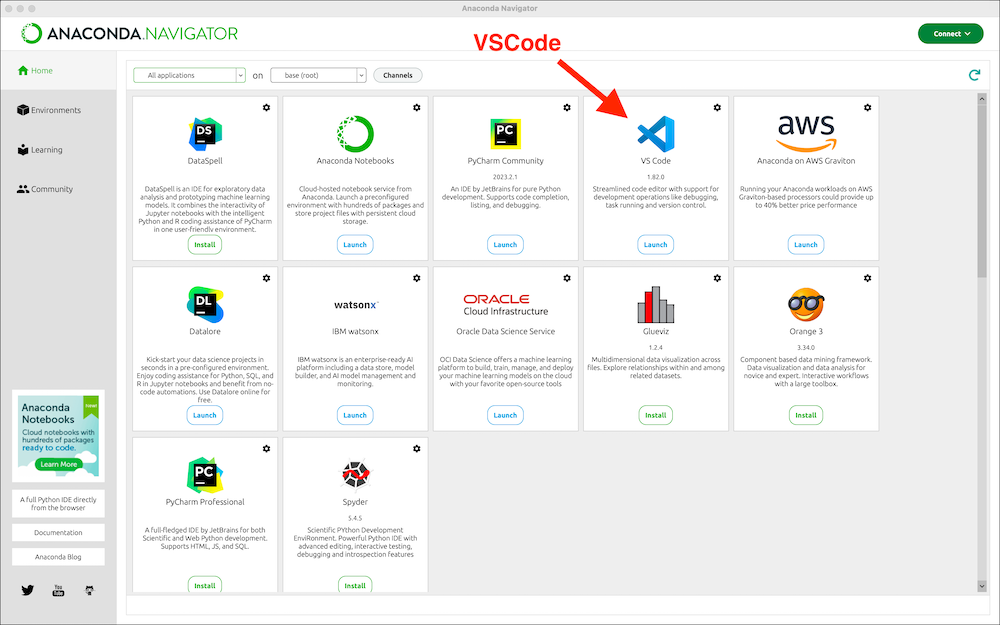
\includegraphics{basics/anaconda-navigator.png}

Sometimes you will need to manualy install the Jupyter extension on
VSCode. In this case follow
\href{https://code.visualstudio.com/docs/datascience/jupyter-notebooks}{this
tutorial}.

\hypertarget{folder-structure}{%
\section{folder structure}\label{folder-structure}}

You \textbf{NEED} to be confortable with you computer's folder (or
directory) structure. Where are files located? How to navigate through
different folders? How is my stuff organized? If you don't feel
\textbf{absolutely} comfortable with this, then read this,
\href{http://www2.westsussex.gov.uk/LearningandDevelopment/IT\%20Learning\%20Guides/Microsoft\%20Windows\%207/05\%20Working\%20with\%20folders.pdf}{Windows},
\href{https://recoverit.wondershare.com/mac-tips/mac-finder-tutorial-mac.html}{MacOS}.
If you use Linux then you surely know this stuff. \textbf{Make yourself
a ``time-series'' folder} wherever you want, and have it backed up
regularly (use Google Drive, Dropbox, do it manually, etc). ``My dog
deleted my files'' is not an excuse.

\hypertarget{numpy-pandas-matplotlib}{%
\chapter{numpy, pandas, matplotlib}\label{numpy-pandas-matplotlib}}

\begin{Shaded}
\begin{Highlighting}[]
\ImportTok{import}\NormalTok{ numpy }\ImportTok{as}\NormalTok{ np}
\ImportTok{import}\NormalTok{ pandas }\ImportTok{as}\NormalTok{ pd}
\ImportTok{import}\NormalTok{ matplotlib.pyplot }\ImportTok{as}\NormalTok{ plt}
\end{Highlighting}
\end{Shaded}

The three lines above are the most common way you will start every
project in this course.

\begin{itemize}
\tightlist
\item
  \textbf{numpy} = numerical python. This library has a ton useful
  mathematical functions, and most importantly, it has an object called
  \texttt{numpy\ array}, which is one of the most useful data structures
  we have for time series analysis.
\item
  \textbf{pandas} is built upon numpy, and allows us to easily
  manipulate data stored in \texttt{dataframes}, a fancy name for a
  table.
\item
  \textbf{pyplot} is a submodule of \texttt{matplotlib}, and allows us
  to beautifully plot data.
\end{itemize}

The best resource I know to get acquainted with all three packages is
\href{https://jakevdp.github.io/PythonDataScienceHandbook/index.html}{Python
Data Science Handbook, by Jake VanderPlas}. This is a free online book,
with excellent step by step examples.

\hypertarget{pandas}{%
\section{pandas}\label{pandas}}

We will primarily use the Pandas package to deal with data. Pandas has
become the standard Python tool to manipulate time series, and you
should get acquainted with its basic usage. This course will provide you
the opportunity to learn by example, but I'm sure we will only scratch
the surface, and you'll be left with lots of questions.

I provide below a (non-comprehensive) list of useful tutorials, they are
a good reference for the beginner and for the experienced user.

\begin{itemize}
\tightlist
\item
  \href{https://jakevdp.github.io/PythonDataScienceHandbook/index.html}{Python
  Data Science Handbook, by Jake VanderPlas}
\item
  \href{https://pandas.pydata.org/Pandas_Cheat_Sheet.pdf}{Data Wrangling
  with pandas Cheat Sheet}
\item
  \href{https://images.datacamp.com/image/upload/v1666944896/Marketing/Blog/Working_with_Dates_and_Times_Cheat_Sheet.pdf}{Working
  with Dates and Times in Python}
\item
  \href{https://www.webpages.uidaho.edu/~stevel/cheatsheets/Pandas\%20DataFrame\%20Notes_12pages.pdf}{Cheat
  Sheet: The pandas DataFrame Object}
\item
  \href{https://www.youtube.com/watch?v=ZyhVh-qRZPA\&list=PL-osiE80TeTsWmV9i9c58mdDCSskIFdDS\&pp=iAQB}{YouTube
  tutorials} by Corey Schafer
\end{itemize}

\hypertarget{pyplot}{%
\section{pyplot}\label{pyplot}}

Matplotlib, and its submodule pyplot, are probably the most common
Python plotting tool. Pyplot is both great and horrible:

\begin{itemize}
\tightlist
\item
  Great: you'll have absolutely full control of everything you want to
  plot. The sky is the limit.
\item
  Horrible: you'll cry as you do it, because there is so much to know,
  and it is not the most friendly plotting package.
\end{itemize}

Pyplot is \emph{object oriented}, so you will usually manipulate the
\textbf{axes} object like this.

\begin{Shaded}
\begin{Highlighting}[]
\ImportTok{import}\NormalTok{ matplotlib.pyplot }\ImportTok{as}\NormalTok{ plt}

\NormalTok{x }\OperatorTok{=}\NormalTok{ [}\DecValTok{1}\NormalTok{, }\DecValTok{2}\NormalTok{, }\DecValTok{3}\NormalTok{, }\DecValTok{4}\NormalTok{, }\DecValTok{5}\NormalTok{]}
\NormalTok{y }\OperatorTok{=}\NormalTok{ [}\DecValTok{1}\NormalTok{, }\DecValTok{4}\NormalTok{, }\DecValTok{2}\NormalTok{, }\DecValTok{0}\NormalTok{, }\DecValTok{3}\NormalTok{]}

\CommentTok{\# Figure with two plots}
\NormalTok{fig, (ax1, ax2) }\OperatorTok{=}\NormalTok{ plt.subplots(}\DecValTok{1}\NormalTok{, }\DecValTok{2}\NormalTok{, figsize }\OperatorTok{=}\NormalTok{ (}\DecValTok{8}\NormalTok{, }\DecValTok{6}\NormalTok{))}
\CommentTok{\# plot on the left}
\NormalTok{ax1.plot(x, y, color}\OperatorTok{=}\StringTok{"tab:blue"}\NormalTok{)}
\NormalTok{ax1.plot(x, y[::}\OperatorTok{{-}}\DecValTok{1}\NormalTok{], color}\OperatorTok{=}\StringTok{"tab:orange"}\NormalTok{)}
\NormalTok{ax1.}\BuiltInTok{set}\NormalTok{(xlabel}\OperatorTok{=}\StringTok{"date"}\NormalTok{,}
\NormalTok{        ylabel}\OperatorTok{=}\StringTok{"something"}\NormalTok{,}
\NormalTok{        title}\OperatorTok{=}\StringTok{"left panel"}\NormalTok{)}
\CommentTok{\# plot on the right}
\NormalTok{ax2.plot(x, y[::}\OperatorTok{{-}}\DecValTok{1}\NormalTok{])}
\NormalTok{ax2.}\BuiltInTok{set}\NormalTok{(xlabel}\OperatorTok{=}\StringTok{"date"}\NormalTok{,}
\NormalTok{        ylabel}\OperatorTok{=}\StringTok{"something else"}\NormalTok{,}
\NormalTok{        title}\OperatorTok{=}\StringTok{"right panel"}\NormalTok{)}
\end{Highlighting}
\end{Shaded}

\begin{verbatim}
[Text(0.5, 0, 'date'),
 Text(0, 0.5, 'something else'),
 Text(0.5, 1.0, 'right panel')]
\end{verbatim}

\begin{figure}[H]

{\centering 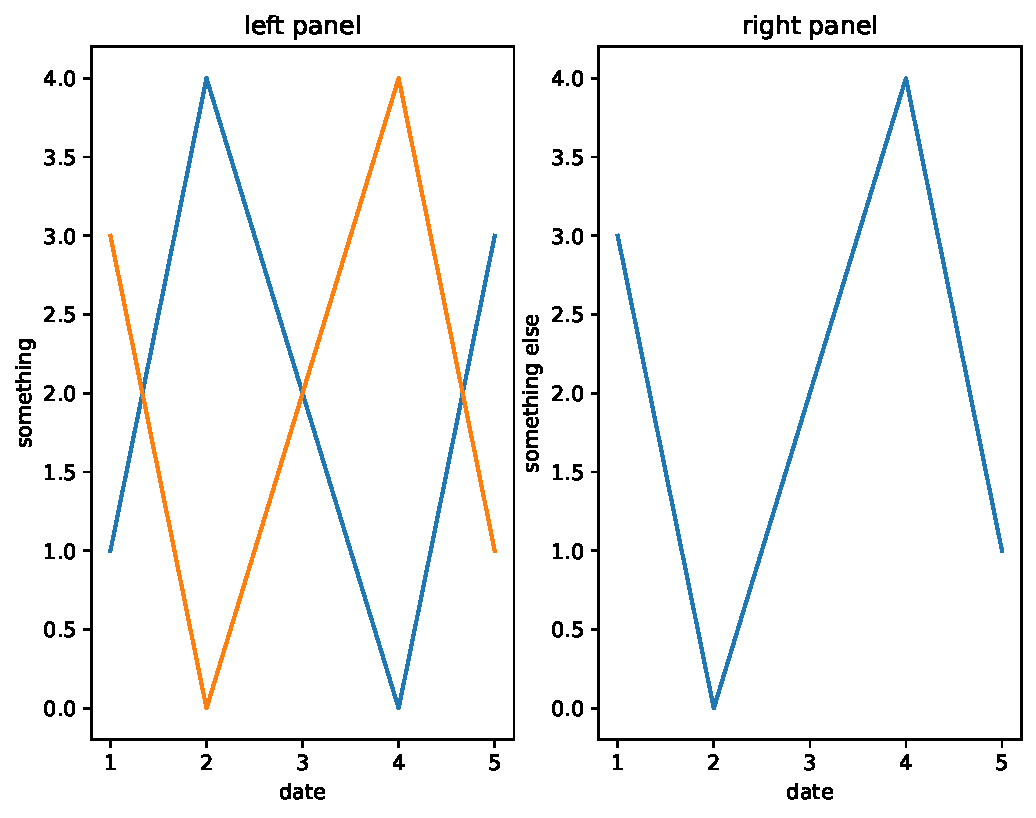
\includegraphics{basics/numpy-pandas-matplotlib_files/figure-pdf/cell-2-output-2.pdf}

}

\end{figure}

For the very beginners, you need to know that \texttt{figure} refers to
the whole white canvas, and \texttt{axes} means the rectangle inside
which something will be plotted:

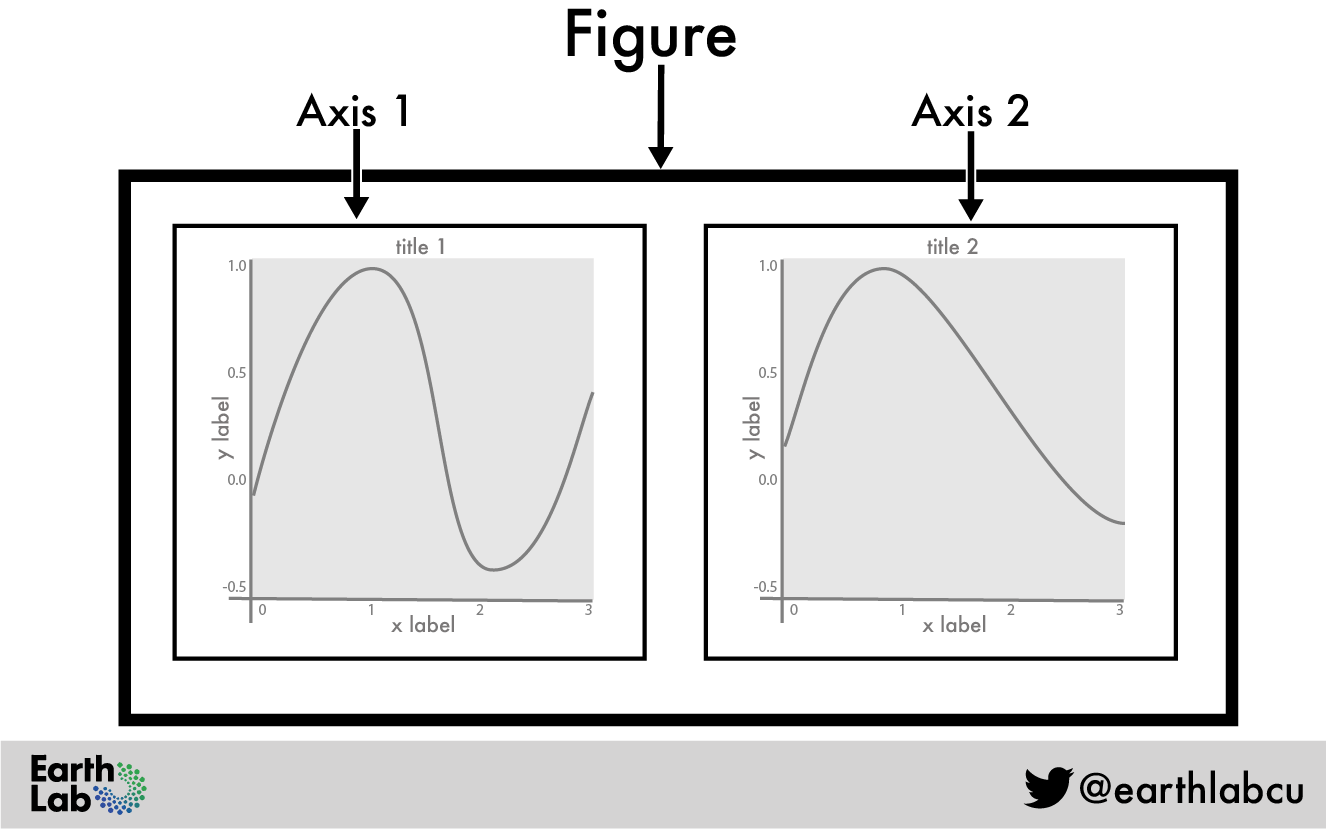
\includegraphics{basics/fig-2-plots.png}

The image above is good because it has 2 panels, and it's easy to
understand what going on. Sadly, they mixed the two terms, axis and
axes.

\begin{itemize}
\tightlist
\item
  \textbf{axes} is where the whole plot will be drawn. In the figure
  above it is the same as each panel.
\item
  \textbf{axis} is each of the vertical and horizontal lines, where you
  have ticks and numbers.
\end{itemize}

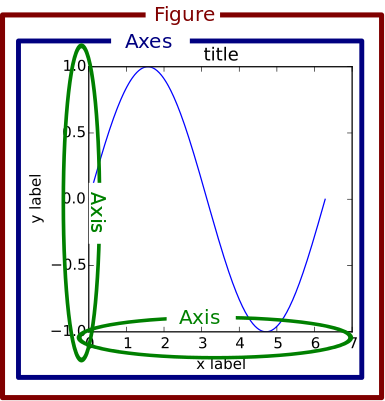
\includegraphics{basics/axis-vs-axes.png}

If you are new to all this, I recommend that you go to:

\begin{itemize}
\tightlist
\item
  \href{https://www.earthdatascience.org/courses/scientists-guide-to-plotting-data-in-python/plot-with-matplotlib/introduction-to-matplotlib-plots/}{Earth
  Lab's Introduction to Plotting in Python Using Matplotlib}
\item
  \href{https://jakevdp.github.io/PythonDataScienceHandbook/index.html}{Jake
  VanderPlas's Python Data Science Handbook}
\end{itemize}

\hypertarget{learn-by-example}{%
\chapter{learn by example}\label{learn-by-example}}

Now that everything is installed, try to run the code below
\emph{before} the first lecture. Don't worry if you don't understand
everything.

\begin{itemize}
\tightlist
\item
  If you manage to run everything without errors, this means that your
  computer is good to go!
\item
  You might encounter a few problems. That's ok. Make a note and we will
  solve everything in the first lecture.
\end{itemize}

Let's make a first plot of real data. We will use NOAA's Global
Monitoring Laboratory data on
\href{https://gml.noaa.gov/ccgg/trends/data.html}{Trends in Atmospheric
Carbon Dioxide}.

\hypertarget{open-a-new-jupyter-notebook}{%
\section{open a new Jupyter
Notebook}\label{open-a-new-jupyter-notebook}}

\begin{enumerate}
\def\labelenumi{\arabic{enumi}.}
\tightlist
\item
  On your computer, open the program \texttt{Anaconda\ Navigator} (it
  may take a while to load).
\item
  Find the white box called \texttt{VS\ Code} and click \texttt{Launch}.
\item
  Now go to \texttt{File} \textgreater{} \texttt{Open\ Folder}, and open
  the folder you created for this course. VS Code may ask you if you
  trust the authors, and the answer is ``yes'' (it's your computer).
\item
  \texttt{File} \textgreater{} \texttt{New\ File}, and call it
  \texttt{example.ipynb}
\item
  You can start copying and pasting code from this website to your
  Jupyter Notebook. To run a cell, press Shift+Enter.
\item
  You may be asked to choose to Select Kernel. This is VS Code wanting
  to know which python installation to use. Click on ``Python
  Environments'', and then choose the option with the word
  \texttt{anaconda} in it.
\item
  That's all! Congratulations!
\end{enumerate}

\hypertarget{import-packages}{%
\section{import packages}\label{import-packages}}

First, import packages to be used. They should all be already included
in the Anaconda distribution you installed.

\begin{Shaded}
\begin{Highlighting}[]
\ImportTok{import}\NormalTok{ numpy }\ImportTok{as}\NormalTok{ np}
\ImportTok{import}\NormalTok{ matplotlib.pyplot }\ImportTok{as}\NormalTok{ plt}
\ImportTok{import}\NormalTok{ pandas }\ImportTok{as}\NormalTok{ pd}
\ImportTok{import}\NormalTok{ seaborn }\ImportTok{as}\NormalTok{ sns}
\NormalTok{sns.}\BuiltInTok{set}\NormalTok{(style}\OperatorTok{=}\StringTok{"ticks"}\NormalTok{, font\_scale}\OperatorTok{=}\FloatTok{1.5}\NormalTok{)  }\CommentTok{\# white graphs, with large and legible letters}
\end{Highlighting}
\end{Shaded}

\hypertarget{load-data}{%
\section{load data}\label{load-data}}

Load CO2 data into a Pandas dataframe. You can load it directly from the
URL (option 1), or first download the CSV to your computer and then load
it (option 2). The link to download the data directly form NOAA is
\href{https://gml.noaa.gov/webdata/ccgg/trends/co2/co2_weekly_mlo.csv}{this}.
If for some reason this doesn't work, download here.

\begin{Shaded}
\begin{Highlighting}[]
\CommentTok{\# option 1: load data directly from URL}
\CommentTok{\# url = "https://gml.noaa.gov/webdata/ccgg/trends/co2/co2\_weekly\_mlo.csv"}
\CommentTok{\# df = pd.read\_csv(url,}
\CommentTok{\#                  header=34,}
\CommentTok{\#                  na\_values=[{-}999.99]}
\CommentTok{\#                  )}

\CommentTok{\# option 2: download first (use the URL above and save it to your computer), then load csv}
\NormalTok{filename }\OperatorTok{=} \StringTok{"co2\_weekly\_mlo.csv"}
\NormalTok{df }\OperatorTok{=}\NormalTok{ pd.read\_csv(filename,}
\NormalTok{                comment}\OperatorTok{=}\StringTok{\textquotesingle{}\#\textquotesingle{}}\NormalTok{,  }\CommentTok{\# will ignore rows starting with \#}
\NormalTok{                 na\_values}\OperatorTok{=}\NormalTok{[}\OperatorTok{{-}}\FloatTok{999.99}\NormalTok{]  }\CommentTok{\# substitute {-}999.99 for NaN (Not a Number), data not available}
\NormalTok{                 )}
\CommentTok{\# check how the dataframe (table) looks like}
\NormalTok{df}
\end{Highlighting}
\end{Shaded}

\begin{longtable}[]{@{}llllllllll@{}}
\toprule\noalign{}
& year & month & day & decimal & average & ndays & 1 year ago & 10 years
ago & increase since 1800 \\
\midrule\noalign{}
\endhead
\bottomrule\noalign{}
\endlastfoot
0 & 1974 & 5 & 19 & 1974.3795 & 333.37 & 5 & NaN & NaN & 50.39 \\
1 & 1974 & 5 & 26 & 1974.3986 & 332.95 & 6 & NaN & NaN & 50.05 \\
2 & 1974 & 6 & 2 & 1974.4178 & 332.35 & 5 & NaN & NaN & 49.59 \\
3 & 1974 & 6 & 9 & 1974.4370 & 332.20 & 7 & NaN & NaN & 49.64 \\
4 & 1974 & 6 & 16 & 1974.4562 & 332.37 & 7 & NaN & NaN & 50.06 \\
... & ... & ... & ... & ... & ... & ... & ... & ... & ... \\
2566 & 2023 & 7 & 23 & 2023.5575 & 421.28 & 4 & 418.03 & 397.30 &
141.60 \\
2567 & 2023 & 7 & 30 & 2023.5767 & 420.83 & 6 & 418.10 & 396.80 &
141.69 \\
2568 & 2023 & 8 & 6 & 2023.5959 & 420.02 & 6 & 417.36 & 395.65 &
141.41 \\
2569 & 2023 & 8 & 13 & 2023.6151 & 418.98 & 4 & 417.25 & 395.24 &
140.89 \\
2570 & 2023 & 8 & 20 & 2023.6342 & 419.31 & 2 & 416.64 & 395.22 &
141.71 \\
\end{longtable}

\hypertarget{dealing-with-dates}{%
\section{dealing with dates}\label{dealing-with-dates}}

Create a new column called \texttt{date}, that combines the information
from three separate columns: \texttt{year}, \texttt{month},
\texttt{day}.

\begin{Shaded}
\begin{Highlighting}[]
\CommentTok{\# function to\_datetime translates the full date into a pandas datetime object,}
\CommentTok{\# that is, pandas knows this is a date, it\textquotesingle{}s not just a string}
\NormalTok{df[}\StringTok{\textquotesingle{}date\textquotesingle{}}\NormalTok{] }\OperatorTok{=}\NormalTok{ pd.to\_datetime(df[[}\StringTok{\textquotesingle{}year\textquotesingle{}}\NormalTok{, }\StringTok{\textquotesingle{}month\textquotesingle{}}\NormalTok{, }\StringTok{\textquotesingle{}day\textquotesingle{}}\NormalTok{]])}
\CommentTok{\# make \textquotesingle{}date\textquotesingle{} column the dataframe index}
\NormalTok{df }\OperatorTok{=}\NormalTok{ df.set\_index(}\StringTok{\textquotesingle{}date\textquotesingle{}}\NormalTok{)}
\CommentTok{\# now see if everything is ok}
\NormalTok{df}
\end{Highlighting}
\end{Shaded}

\begin{longtable}[]{@{}llllllllll@{}}
\toprule\noalign{}
& year & month & day & decimal & average & ndays & 1 year ago & 10 years
ago & increase since 1800 \\
date & & & & & & & & & \\
\midrule\noalign{}
\endhead
\bottomrule\noalign{}
\endlastfoot
1974-05-19 & 1974 & 5 & 19 & 1974.3795 & 333.37 & 5 & NaN & NaN &
50.39 \\
1974-05-26 & 1974 & 5 & 26 & 1974.3986 & 332.95 & 6 & NaN & NaN &
50.05 \\
1974-06-02 & 1974 & 6 & 2 & 1974.4178 & 332.35 & 5 & NaN & NaN &
49.59 \\
1974-06-09 & 1974 & 6 & 9 & 1974.4370 & 332.20 & 7 & NaN & NaN &
49.64 \\
1974-06-16 & 1974 & 6 & 16 & 1974.4562 & 332.37 & 7 & NaN & NaN &
50.06 \\
... & ... & ... & ... & ... & ... & ... & ... & ... & ... \\
2023-07-23 & 2023 & 7 & 23 & 2023.5575 & 421.28 & 4 & 418.03 & 397.30 &
141.60 \\
2023-07-30 & 2023 & 7 & 30 & 2023.5767 & 420.83 & 6 & 418.10 & 396.80 &
141.69 \\
2023-08-06 & 2023 & 8 & 6 & 2023.5959 & 420.02 & 6 & 417.36 & 395.65 &
141.41 \\
2023-08-13 & 2023 & 8 & 13 & 2023.6151 & 418.98 & 4 & 417.25 & 395.24 &
140.89 \\
2023-08-20 & 2023 & 8 & 20 & 2023.6342 & 419.31 & 2 & 416.64 & 395.22 &
141.71 \\
\end{longtable}

\hypertarget{first-plot}{%
\section{first plot}\label{first-plot}}

We are now ready for our first plot! Let's see the weekly CO2 average.

\begin{Shaded}
\begin{Highlighting}[]
\CommentTok{\# \%matplotlib widget}
\CommentTok{\# uncomment the above line if you want dynamic control of the figure when using VSCode}
\NormalTok{fig, (ax1, ax2) }\OperatorTok{=}\NormalTok{ plt.subplots(}\DecValTok{1}\NormalTok{, }\DecValTok{2}\NormalTok{,  }\CommentTok{\# 1 row, 2 columns}
\NormalTok{                               figsize}\OperatorTok{=}\NormalTok{(}\DecValTok{8}\NormalTok{,}\DecValTok{5}\NormalTok{)  }\CommentTok{\# width, height, in inches}
\NormalTok{                               )}
\CommentTok{\# left panel}
\NormalTok{ax1.plot(df[}\StringTok{\textquotesingle{}average\textquotesingle{}}\NormalTok{], color}\OperatorTok{=}\StringTok{"black"}\NormalTok{)}
\NormalTok{ax1.plot(df.loc[}\StringTok{\textquotesingle{}2010{-}01{-}01\textquotesingle{}}\NormalTok{:}\StringTok{\textquotesingle{}2011{-}12{-}31\textquotesingle{}}\NormalTok{,}\StringTok{\textquotesingle{}average\textquotesingle{}}\NormalTok{], color}\OperatorTok{=}\StringTok{"magenta"}\NormalTok{)}
\NormalTok{ax1.}\BuiltInTok{set}\NormalTok{(xlabel}\OperatorTok{=}\StringTok{"date"}\NormalTok{,}
\NormalTok{       ylabel}\OperatorTok{=}\VerbatimStringTok{r"CO$\_2$ concentration (ppm)"}\NormalTok{,}
\NormalTok{       title}\OperatorTok{=}\StringTok{"long term"}\NormalTok{)}\OperatorTok{;}
\CommentTok{\# right panel}
\NormalTok{ax2.plot(df.loc[}\StringTok{\textquotesingle{}2010{-}01{-}01\textquotesingle{}}\NormalTok{:}\StringTok{\textquotesingle{}2011{-}12{-}31\textquotesingle{}}\NormalTok{,}\StringTok{\textquotesingle{}average\textquotesingle{}}\NormalTok{], color}\OperatorTok{=}\StringTok{"magenta"}\NormalTok{)}
\NormalTok{ax2.}\BuiltInTok{set}\NormalTok{(xlabel}\OperatorTok{=}\StringTok{"date"}\NormalTok{,}
\NormalTok{        ylabel}\OperatorTok{=}\VerbatimStringTok{r"CO$\_2$ concentration (ppm)"}\NormalTok{,}
\NormalTok{        ylim}\OperatorTok{=}\NormalTok{[}\DecValTok{385}\NormalTok{, }\DecValTok{400}\NormalTok{],  }\CommentTok{\# choose y limits}
\NormalTok{        yticks}\OperatorTok{=}\NormalTok{np.arange(}\DecValTok{385}\NormalTok{, }\DecValTok{401}\NormalTok{, }\DecValTok{5}\NormalTok{),  }\CommentTok{\# choose ticks}
\NormalTok{        title}\OperatorTok{=}\StringTok{"years 2010{-}{-}2011"}\NormalTok{)}\OperatorTok{;}
\CommentTok{\# put ticks and label on the right for ax2}
\NormalTok{ax2.yaxis.tick\_right()}
\NormalTok{ax2.yaxis.set\_label\_position(}\StringTok{"right"}\NormalTok{)}
\CommentTok{\# title above both panels}
\NormalTok{fig.suptitle(}\StringTok{"Mauna Loa Observatory"}\NormalTok{)}
\CommentTok{\# makes slanted dates}
\NormalTok{plt.gcf().autofmt\_xdate()}
\end{Highlighting}
\end{Shaded}

\begin{figure}[H]

{\centering \includegraphics{basics/example_files/figure-pdf/cell-5-output-1.png}

}

\end{figure}

\hypertarget{first-plot-v2.0}{%
\section{first plot, v2.0}\label{first-plot-v2.0}}

The dates in the x-label are not great. Let's try to make them prettier.

We need to import a few more packages first.

\begin{Shaded}
\begin{Highlighting}[]
\ImportTok{import}\NormalTok{ matplotlib.dates }\ImportTok{as}\NormalTok{ mdates}
\ImportTok{from}\NormalTok{ matplotlib.dates }\ImportTok{import}\NormalTok{ DateFormatter}
\ImportTok{from}\NormalTok{ pandas.plotting }\ImportTok{import}\NormalTok{ register\_matplotlib\_converters}
\NormalTok{register\_matplotlib\_converters()  }\CommentTok{\# datetime converter for a matplotlib}
\end{Highlighting}
\end{Shaded}

Now let's replot.

\begin{Shaded}
\begin{Highlighting}[]
\CommentTok{\# \%matplotlib widget}
\CommentTok{\# uncomment the above line if you want dynamic control of the figure when using VSCode}
\NormalTok{fig, (ax1, ax2) }\OperatorTok{=}\NormalTok{ plt.subplots(}\DecValTok{1}\NormalTok{, }\DecValTok{2}\NormalTok{,  }\CommentTok{\# 1 row, 2 columns}
\NormalTok{                               figsize}\OperatorTok{=}\NormalTok{(}\DecValTok{8}\NormalTok{,}\DecValTok{5}\NormalTok{)  }\CommentTok{\# width, height, in inches}
\NormalTok{                               )}
\CommentTok{\# left panel}
\NormalTok{ax1.plot(df[}\StringTok{\textquotesingle{}average\textquotesingle{}}\NormalTok{], color}\OperatorTok{=}\StringTok{"black"}\NormalTok{)}
\NormalTok{ax1.plot(df.loc[}\StringTok{\textquotesingle{}2010{-}01{-}01\textquotesingle{}}\NormalTok{:}\StringTok{\textquotesingle{}2011{-}12{-}31\textquotesingle{}}\NormalTok{,}\StringTok{\textquotesingle{}average\textquotesingle{}}\NormalTok{], color}\OperatorTok{=}\StringTok{"magenta"}\NormalTok{)}
\NormalTok{ax1.}\BuiltInTok{set}\NormalTok{(xlabel}\OperatorTok{=}\StringTok{"date"}\NormalTok{,}
\NormalTok{       ylabel}\OperatorTok{=}\VerbatimStringTok{r"CO$\_2$ concentration (ppm)"}\NormalTok{,}
\NormalTok{       title}\OperatorTok{=}\StringTok{"long term"}\NormalTok{)}\OperatorTok{;}
\CommentTok{\# right panel}
\NormalTok{ax2.plot(df.loc[}\StringTok{\textquotesingle{}2010{-}01{-}01\textquotesingle{}}\NormalTok{:}\StringTok{\textquotesingle{}2011{-}12{-}31\textquotesingle{}}\NormalTok{,}\StringTok{\textquotesingle{}average\textquotesingle{}}\NormalTok{], color}\OperatorTok{=}\StringTok{"magenta"}\NormalTok{)}
\NormalTok{ax2.}\BuiltInTok{set}\NormalTok{(xlabel}\OperatorTok{=}\StringTok{"date"}\NormalTok{,}
\NormalTok{        ylabel}\OperatorTok{=}\VerbatimStringTok{r"CO$\_2$ concentration (ppm)"}\NormalTok{,}
\NormalTok{        ylim}\OperatorTok{=}\NormalTok{[}\DecValTok{385}\NormalTok{, }\DecValTok{400}\NormalTok{],  }\CommentTok{\# choose y limits}
\NormalTok{        yticks}\OperatorTok{=}\NormalTok{np.arange(}\DecValTok{385}\NormalTok{, }\DecValTok{401}\NormalTok{, }\DecValTok{5}\NormalTok{),  }\CommentTok{\# choose ticks}
\NormalTok{        title}\OperatorTok{=}\StringTok{"years 2010{-}{-}2011"}\NormalTok{)}\OperatorTok{;}
\CommentTok{\# put ticks and label on the right for ax2}
\NormalTok{ax2.yaxis.tick\_right()}
\NormalTok{ax2.yaxis.set\_label\_position(}\StringTok{"right"}\NormalTok{)}
\CommentTok{\# title above both panels}
\NormalTok{fig.suptitle(}\StringTok{"Mauna Loa Observatory"}\NormalTok{, y}\OperatorTok{=}\FloatTok{1.00}\NormalTok{)}

\NormalTok{locator }\OperatorTok{=}\NormalTok{ mdates.AutoDateLocator(minticks}\OperatorTok{=}\DecValTok{3}\NormalTok{, maxticks}\OperatorTok{=}\DecValTok{5}\NormalTok{)}
\NormalTok{formatter }\OperatorTok{=}\NormalTok{ mdates.ConciseDateFormatter(locator)}
\NormalTok{ax1.xaxis.set\_major\_locator(locator)}
\NormalTok{ax1.xaxis.set\_major\_formatter(formatter)}

\NormalTok{locator }\OperatorTok{=}\NormalTok{ mdates.AutoDateLocator(minticks}\OperatorTok{=}\DecValTok{4}\NormalTok{, maxticks}\OperatorTok{=}\DecValTok{5}\NormalTok{)}
\NormalTok{formatter }\OperatorTok{=}\NormalTok{ mdates.ConciseDateFormatter(locator)}
\NormalTok{ax2.xaxis.set\_major\_locator(locator)}
\NormalTok{ax2.xaxis.set\_major\_formatter(formatter)}

\NormalTok{ax1.annotate(}
    \StringTok{"2010/11"}\NormalTok{,}
\NormalTok{    xy}\OperatorTok{=}\NormalTok{(}\StringTok{\textquotesingle{}2011{-}12{-}25\textquotesingle{}}\NormalTok{, }\DecValTok{389}\NormalTok{),  xycoords}\OperatorTok{=}\StringTok{\textquotesingle{}data\textquotesingle{}}\NormalTok{,}
\NormalTok{    xytext}\OperatorTok{=}\NormalTok{(}\OperatorTok{{-}}\DecValTok{10}\NormalTok{, }\OperatorTok{{-}}\DecValTok{80}\NormalTok{), textcoords}\OperatorTok{=}\StringTok{\textquotesingle{}offset points\textquotesingle{}}\NormalTok{,}
\NormalTok{    arrowprops}\OperatorTok{=}\BuiltInTok{dict}\NormalTok{(arrowstyle}\OperatorTok{=}\StringTok{"{-}\textgreater{}"}\NormalTok{,}
\NormalTok{                    color}\OperatorTok{=}\StringTok{"black"}\NormalTok{,}
\NormalTok{                    connectionstyle}\OperatorTok{=}\StringTok{"arc3,rad=0.2"}\NormalTok{))}
\NormalTok{fig.savefig(}\StringTok{"CO2{-}graph.png"}\NormalTok{, dpi}\OperatorTok{=}\DecValTok{300}\NormalTok{)}
\end{Highlighting}
\end{Shaded}

\begin{verbatim}
/var/folders/hc/jhnmlst937d27zzq9fhfks780000gn/T/ipykernel_10652/850389963.py:42: UserWarning: AutoDateLocator was unable to pick an appropriate interval for this date range. It may be necessary to add an interval value to the AutoDateLocator's intervald dictionary. Defaulting to 6.
  fig.savefig("CO2-graph.png", dpi=300)
/opt/anaconda3/lib/python3.9/site-packages/IPython/core/pylabtools.py:151: UserWarning: AutoDateLocator was unable to pick an appropriate interval for this date range. It may be necessary to add an interval value to the AutoDateLocator's intervald dictionary. Defaulting to 6.
  fig.canvas.print_figure(bytes_io, **kw)
\end{verbatim}

\begin{figure}[H]

{\centering \includegraphics{basics/example_files/figure-pdf/cell-7-output-2.png}

}

\end{figure}

The dates on the horizontal axis are determined thus:

\begin{enumerate}
\def\labelenumi{\arabic{enumi}.}
\tightlist
\item
  \texttt{locator\ =\ mdates.AutoDateLocator(minticks=3,\ maxticks=5)}\strut \\
  This deremines the location of the ticks (between 3 and 5 ticks,
  whatever ``works best'')
\item
  \texttt{ax1.xaxis.set\_major\_locator(locator)}\strut \\
  This actually puts the ticks in the positions determined above
\item
  \texttt{formatter\ =\ mdates.ConciseDateFormatter(locator)}\strut \\
  This says that the labels will be placed at the locations determined
  in 1.
\item
  \texttt{ax1.xaxis.set\_major\_formatter(formatter)}\strut \\
  Finally, labels are written down
\end{enumerate}

The arrow is placed in the graph using \texttt{annotate}. It has a
tricky syntax and a million options. Read
\href{https://jakevdp.github.io/PythonDataScienceHandbook/04.09-text-and-annotation.html\#Arrows-and-Annotation}{Jake
VanderPlas's} excellent examples to learn more.

\hypertarget{modifications}{%
\section{modifications}\label{modifications}}

Let's change a lot of plotting options to see how things could be
different.

\begin{Shaded}
\begin{Highlighting}[]
\NormalTok{sns.}\BuiltInTok{set}\NormalTok{(style}\OperatorTok{=}\StringTok{"darkgrid"}\NormalTok{)}
\NormalTok{sns.set\_context(}\StringTok{"notebook"}\NormalTok{)}

\CommentTok{\# \%matplotlib widget}
\CommentTok{\# uncomment the above line if you want dynamic control of the figure when using VSCode}
\NormalTok{fig, (ax1, ax2) }\OperatorTok{=}\NormalTok{ plt.subplots(}\DecValTok{1}\NormalTok{, }\DecValTok{2}\NormalTok{,  }\CommentTok{\# 1 row, 2 columns}
\NormalTok{                               figsize}\OperatorTok{=}\NormalTok{(}\DecValTok{8}\NormalTok{,}\DecValTok{4}\NormalTok{)  }\CommentTok{\# width, height, in inches}
\NormalTok{                               )}
\CommentTok{\# left panel}
\NormalTok{ax1.plot(df[}\StringTok{\textquotesingle{}average\textquotesingle{}}\NormalTok{], color}\OperatorTok{=}\StringTok{"tab:blue"}\NormalTok{)}
\NormalTok{ax1.plot(df.loc[}\StringTok{\textquotesingle{}2010{-}01{-}01\textquotesingle{}}\NormalTok{:}\StringTok{\textquotesingle{}2011{-}12{-}31\textquotesingle{}}\NormalTok{,}\StringTok{\textquotesingle{}average\textquotesingle{}}\NormalTok{], color}\OperatorTok{=}\StringTok{"tab:orange"}\NormalTok{)}
\NormalTok{ax1.}\BuiltInTok{set}\NormalTok{(xlabel}\OperatorTok{=}\StringTok{"date"}\NormalTok{,}
\NormalTok{       ylabel}\OperatorTok{=}\VerbatimStringTok{r"CO$\_2$ concentration (ppm)"}\NormalTok{,}
\NormalTok{       title}\OperatorTok{=}\StringTok{"long term"}\NormalTok{)}\OperatorTok{;}
\CommentTok{\# right panel}
\NormalTok{ax2.plot(df.loc[}\StringTok{\textquotesingle{}2010{-}01{-}01\textquotesingle{}}\NormalTok{:}\StringTok{\textquotesingle{}2011{-}12{-}31\textquotesingle{}}\NormalTok{,}\StringTok{\textquotesingle{}average\textquotesingle{}}\NormalTok{], color}\OperatorTok{=}\StringTok{"tab:orange"}\NormalTok{)}
\NormalTok{ax2.}\BuiltInTok{set}\NormalTok{(xlabel}\OperatorTok{=}\StringTok{"date"}\NormalTok{,}
\NormalTok{        ylim}\OperatorTok{=}\NormalTok{[}\DecValTok{385}\NormalTok{, }\DecValTok{400}\NormalTok{],  }\CommentTok{\# choose y limits}
\NormalTok{        yticks}\OperatorTok{=}\NormalTok{np.arange(}\DecValTok{385}\NormalTok{, }\DecValTok{401}\NormalTok{, }\DecValTok{5}\NormalTok{),  }\CommentTok{\# choose ticks}
\NormalTok{        title}\OperatorTok{=}\StringTok{"years 2010{-}{-}2011"}\NormalTok{)}\OperatorTok{;}
\CommentTok{\# title above both panels}
\NormalTok{fig.suptitle(}\StringTok{"Mauna Loa Observatory"}\NormalTok{, y}\OperatorTok{=}\FloatTok{1.00}\NormalTok{)}

\NormalTok{locator }\OperatorTok{=}\NormalTok{ mdates.AutoDateLocator(minticks}\OperatorTok{=}\DecValTok{3}\NormalTok{, maxticks}\OperatorTok{=}\DecValTok{5}\NormalTok{)}
\NormalTok{formatter }\OperatorTok{=}\NormalTok{ mdates.ConciseDateFormatter(locator)}
\NormalTok{ax1.xaxis.set\_major\_locator(locator)}
\NormalTok{ax1.xaxis.set\_major\_formatter(formatter)}

\NormalTok{locator }\OperatorTok{=}\NormalTok{ mdates.AutoDateLocator(minticks}\OperatorTok{=}\DecValTok{5}\NormalTok{, maxticks}\OperatorTok{=}\DecValTok{8}\NormalTok{)}
\NormalTok{formatter }\OperatorTok{=}\NormalTok{ mdates.ConciseDateFormatter(locator)}
\NormalTok{ax2.xaxis.set\_major\_locator(locator)}
\NormalTok{ax2.xaxis.set\_major\_formatter(formatter)}

\NormalTok{ax1.annotate(}
    \StringTok{"2010/11"}\NormalTok{,}
\NormalTok{    xy}\OperatorTok{=}\NormalTok{(}\StringTok{\textquotesingle{}2010{-}12{-}25\textquotesingle{}}\NormalTok{, }\DecValTok{395}\NormalTok{),  xycoords}\OperatorTok{=}\StringTok{\textquotesingle{}data\textquotesingle{}}\NormalTok{,}
\NormalTok{    xytext}\OperatorTok{=}\NormalTok{(}\OperatorTok{{-}}\DecValTok{100}\NormalTok{, }\DecValTok{40}\NormalTok{), textcoords}\OperatorTok{=}\StringTok{\textquotesingle{}offset points\textquotesingle{}}\NormalTok{,}
\NormalTok{    bbox}\OperatorTok{=}\BuiltInTok{dict}\NormalTok{(boxstyle}\OperatorTok{=}\StringTok{"round4,pad=.5"}\NormalTok{, fc}\OperatorTok{=}\StringTok{"white"}\NormalTok{),}
\NormalTok{    arrowprops}\OperatorTok{=}\BuiltInTok{dict}\NormalTok{(arrowstyle}\OperatorTok{=}\StringTok{"{-}\textgreater{}"}\NormalTok{,}
\NormalTok{                    color}\OperatorTok{=}\StringTok{"black"}\NormalTok{,}
\NormalTok{                    connectionstyle}\OperatorTok{=}\StringTok{"angle,angleA=0,angleB={-}90,rad=40"}\NormalTok{))}
\end{Highlighting}
\end{Shaded}

\begin{verbatim}
Text(-100, 40, '2010/11')
\end{verbatim}

\begin{figure}[H]

{\centering 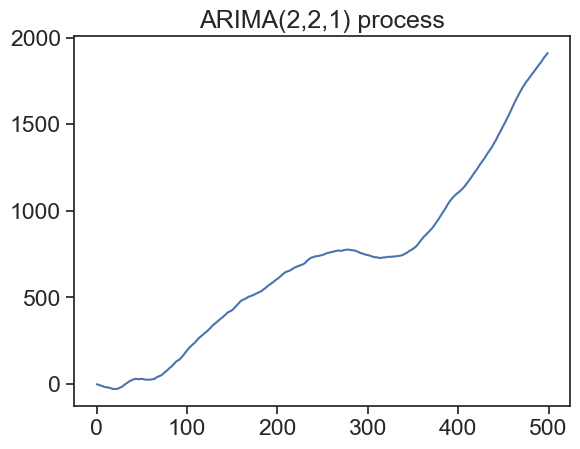
\includegraphics{basics/example_files/figure-pdf/cell-8-output-2.png}

}

\end{figure}

The main changes were:

\begin{enumerate}
\def\labelenumi{\arabic{enumi}.}
\tightlist
\item
  Using the Seaborn package, we changed the fontsize and the overall
  plot style.
  \href{https://seaborn.pydata.org/tutorial/aesthetics.html}{Read
  more}.\\
  \texttt{sns.set(style="darkgrid")}\strut \\
  \texttt{sns.set\_context("notebook")}
\item
  We changed the colors of the lineplots. To know what colors exist,
  \href{https://matplotlib.org/stable/gallery/color/named_colors.html}{click
  here}.
\item
  The arrow annotation has a different style.
  \href{https://jakevdp.github.io/PythonDataScienceHandbook/04.09-text-and-annotation.html\#Arrows-and-Annotation}{Read
  more}.
\end{enumerate}

\hypertarget{playing-with-the-code}{%
\section{playing with the code}\label{playing-with-the-code}}

I encourage you to play with the code you just ran. An easy way of
learning what each line does is to comment something out and see what
changes in the output you see. If you feel brave, try to modify the code
a little bit.

\hypertarget{ai-policy}{%
\chapter{AI policy}\label{ai-policy}}

\begin{figure}

{\centering 
\includegraphics[width=1.04167in,height=\textheight]{basics/robot-scratching_transparent3.png}

}

\end{figure}

The guidelines below are an adaptation of
\href{https://oneusefulthing.substack.com/p/all-my-classes-suddenly-became-ai}{Ethan
Mollick's extremely useful ideas on AI} as an assistant tool for
teaching.

\textbf{I EXPECT YOU} to use LLMs (large language models) such as
ChatGPT, Bing AI, Google Bard, or whatever else springs up since the
time of this writing. You should familiarize yourself with the AI's
capabilities and limitations.

\textbf{Use LLMs to help you learn}, chat with them about what you want
to accomplish and learn from them how to do it. \textbf{Ask} your LLM
what each part of the code means, copy and pasting blindly is
unacceptable. You are here to learn.

Consider the following important points:

\begin{itemize}
\tightlist
\item
  Ultimately, you, the student, are responsible for the assignment.
\item
  Acknowledge the use of AI in your assignment. Be transparent about
  your use of the tool and the extent of assistance it provided.
\end{itemize}

\begin{figure}

{\centering 
\includegraphics{basics/ai-meme1.png}

}

\end{figure}

\part{resampling}

\hypertarget{motivation}{%
\chapter{motivation}\label{motivation}}

\hypertarget{jerusalem-2019}{%
\section{Jerusalem, 2019}\label{jerusalem-2019}}

Data from the \href{https://ims.gov.il/en/data_gov}{Israel
Meteorological Service}, IMS.

See the temperature at a weather station in Jerusalem, for the whole
2019 year. This is an interactive graph: to zoom in, play with the
bottom panel.

\begin{verbatim}
alt.VConcatChart(...)
\end{verbatim}

\hypertarget{iconify-cil-chat-bubble-discussion}{%
\paragraph*{\texorpdfstring{
discussion}{ discussion}}\label{iconify-cil-chat-bubble-discussion}}
\addcontentsline{toc}{paragraph}{ discussion}

The temperature fluctuates on various time scales, from daily to yearly.
Let's think together a few questions we'd like to ask about the data
above.

Now let's see precipitation data:

\begin{verbatim}
alt.VConcatChart(...)
\end{verbatim}

\hypertarget{iconify-cil-chat-bubble-discussion-1}{%
\paragraph*{\texorpdfstring{
discussion}{ discussion}}\label{iconify-cil-chat-bubble-discussion-1}}
\addcontentsline{toc}{paragraph}{ discussion}

What would be interesting to know about precipitation?

We have not talked about what kind of data we have in our hands here.
The csv file provided by the IMS looks like this:

\begin{longtable}[]{@{}lllllllllllllllllll@{}}
\toprule\noalign{}
& Station & Date \& Time (Winter) & Diffused radiation (W/m\^{}2) &
Global radiation (W/m\^{}2) & Direct radiation (W/m\^{}2) & Relative
humidity (\%) & Temperature (°C) & Maximum temperature (°C) & Minimum
temperature (°C) & Wind direction (°) & Gust wind direction (°) & Wind
speed (m/s) & Maximum 1 minute wind speed (m/s) & Maximum 10 minutes
wind speed (m/s) & Time ending maximum 10 minutes wind speed (hhmm) &
Gust wind speed (m/s) & Standard deviation wind direction (°) & Rainfall
(mm) \\
\midrule\noalign{}
\endhead
\bottomrule\noalign{}
\endlastfoot
0 & Jerusalem Givat Ram & 01/01/2019 00:00 & 0.0 & 0.0 & 0.0 & 80.0 &
8.7 & 8.8 & 8.6 & 75.0 & 84.0 & 3.3 & 4.3 & 3.5 & 23:58 & 6.0 & 15.6 &
0.0 \\
1 & Jerusalem Givat Ram & 01/01/2019 00:10 & 0.0 & 0.0 & 0.0 & 79.0 &
8.7 & 8.8 & 8.7 & 74.0 & 82.0 & 3.3 & 4.1 & 3.3 & 00:01 & 4.9 & 14.3 &
0.0 \\
2 & Jerusalem Givat Ram & 01/01/2019 00:20 & 0.0 & 0.0 & 0.0 & 79.0 &
8.7 & 8.8 & 8.7 & 76.0 & 82.0 & 3.2 & 4.1 & 3.3 & 00:19 & 4.9 & 9.9 &
0.0 \\
3 & Jerusalem Givat Ram & 01/01/2019 00:30 & 0.0 & 0.0 & 0.0 & 79.0 &
8.7 & 8.7 & 8.6 & 78.0 & 73.0 & 3.6 & 4.2 & 3.6 & 00:30 & 5.2 & 11.7 &
0.0 \\
4 & Jerusalem Givat Ram & 01/01/2019 00:40 & 0.0 & 0.0 & 0.0 & 79.0 &
8.6 & 8.7 & 8.5 & 80.0 & 74.0 & 3.6 & 4.4 & 3.8 & 00:35 & 5.4 & 10.5 &
0.0 \\
... & ... & ... & ... & ... & ... & ... & ... & ... & ... & ... & ... &
... & ... & ... & ... & ... & ... & ... \\
52549 & Jerusalem Givat Ram & 31/12/2019 22:20 & 0.0 & 0.0 & 1.0 & 81.0
& 7.4 & 7.6 & 7.3 & 222.0 & 255.0 & 0.5 & 0.9 & 1.0 & 22:11 & 1.0 & 47.9
& 0.0 \\
52550 & Jerusalem Givat Ram & 31/12/2019 22:30 & 0.0 & 0.0 & 1.0 & 83.0
& 7.3 & 7.4 & 7.3 & 266.0 & 259.0 & 0.6 & 0.8 & 0.6 & 22:28 & 1.1 & 22.8
& 0.0 \\
52551 & Jerusalem Givat Ram & 31/12/2019 22:40 & 0.0 & 0.0 & 1.0 & 83.0
& 7.5 & 7.6 & 7.3 & 331.0 & 317.0 & 0.5 & 0.8 & 0.6 & 22:35 & 1.0 & 31.6
& 0.0 \\
52552 & Jerusalem Givat Ram & 31/12/2019 22:50 & 0.0 & 0.0 & 1.0 & 83.0
& 7.5 & 7.6 & 7.4 & 312.0 & 285.0 & 0.6 & 1.0 & 0.6 & 22:50 & 1.4 & 31.3
& 0.0 \\
52553 & Jerusalem Givat Ram & 31/12/2019 23:00 & 0.0 & 0.0 & 1.0 & 83.0
& 7.6 & 7.7 & 7.4 & 315.0 & 321.0 & 0.7 & 1.0 & 0.8 & 22:54 & 1.3 & 23.5
& 0.0 \\
\end{longtable}

We see that we have data points spaced out evenly every 10 minutes.

\hypertarget{challenges}{%
\section{Challenges}\label{challenges}}

Let's try to answer the following questions:

\begin{tcolorbox}[enhanced jigsaw, titlerule=0mm, title={What is the mean temperature for each month?}, coltitle=black, colframe=quarto-callout-note-color-frame, toprule=.15mm, bottomrule=.15mm, bottomtitle=1mm, colbacktitle=quarto-callout-note-color!10!white, toptitle=1mm, breakable, arc=.35mm, colback=white, opacityback=0, left=2mm, leftrule=.75mm, rightrule=.15mm, opacitybacktitle=0.6]

First we have to divide temperature data by month, and then take the
average for each month.

a possible solution

\begin{Shaded}
\begin{Highlighting}[]
\NormalTok{df\_month }\OperatorTok{=}\NormalTok{ df[}\StringTok{\textquotesingle{}temperature\textquotesingle{}}\NormalTok{].resample(}\StringTok{\textquotesingle{}M\textquotesingle{}}\NormalTok{).mean()}
\end{Highlighting}
\end{Shaded}

\end{tcolorbox}

\begin{tcolorbox}[enhanced jigsaw, titlerule=0mm, title={For each month, what is the mean of the daily maximum temperature? What
about the minimun?}, coltitle=black, colframe=quarto-callout-note-color-frame, toprule=.15mm, bottomrule=.15mm, bottomtitle=1mm, colbacktitle=quarto-callout-note-color!10!white, toptitle=1mm, breakable, arc=.35mm, colback=white, opacityback=0, left=2mm, leftrule=.75mm, rightrule=.15mm, opacitybacktitle=0.6]

This is a bit trickier.

\begin{enumerate}
\def\labelenumi{\arabic{enumi}.}
\tightlist
\item
  We need to find the maximum/minimum temperature for each day.
\item
  Only then we split the daily data by month and take the average.
\end{enumerate}

a possible solution

\begin{Shaded}
\begin{Highlighting}[]
\NormalTok{df\_day[}\StringTok{\textquotesingle{}max temp\textquotesingle{}}\NormalTok{] }\OperatorTok{=}\NormalTok{ df[}\StringTok{\textquotesingle{}temperature\textquotesingle{}}\NormalTok{].resample(}\StringTok{\textquotesingle{}D\textquotesingle{}}\NormalTok{).}\BuiltInTok{max}\NormalTok{()}
\NormalTok{df\_month[}\StringTok{\textquotesingle{}max temp\textquotesingle{}}\NormalTok{] }\OperatorTok{=}\NormalTok{ df\_day[}\StringTok{\textquotesingle{}max temp\textquotesingle{}}\NormalTok{].resample(}\StringTok{\textquotesingle{}MS\textquotesingle{}}\NormalTok{).mean()}
\end{Highlighting}
\end{Shaded}

\end{tcolorbox}

\begin{tcolorbox}[enhanced jigsaw, titlerule=0mm, title={What is the average night temperature for every season? What about the
day temperature?}, coltitle=black, colframe=quarto-callout-note-color-frame, toprule=.15mm, bottomrule=.15mm, bottomtitle=1mm, colbacktitle=quarto-callout-note-color!10!white, toptitle=1mm, breakable, arc=.35mm, colback=white, opacityback=0, left=2mm, leftrule=.75mm, rightrule=.15mm, opacitybacktitle=0.6]

\begin{enumerate}
\def\labelenumi{\arabic{enumi}.}
\tightlist
\item
  We need to filter our data to contain only night times.
\item
  We need to divide rain data by seasons (3 months), and then take the
  mean for each season.
\end{enumerate}

a possible solution

\begin{Shaded}
\begin{Highlighting}[]
\CommentTok{\# filter only night data}
\NormalTok{df\_night }\OperatorTok{=}\NormalTok{ df.loc[((df.index.hour }\OperatorTok{\textless{}} \DecValTok{6}\NormalTok{) }\OperatorTok{|}\NormalTok{ (df.index.hour }\OperatorTok{\textgreater{}=} \DecValTok{18}\NormalTok{))]}
\NormalTok{season\_average\_night\_temp }\OperatorTok{=}\NormalTok{ df\_night[}\StringTok{\textquotesingle{}temperature\textquotesingle{}}\NormalTok{].resample(}\StringTok{\textquotesingle{}Q\textquotesingle{}}\NormalTok{).mean()}
\end{Highlighting}
\end{Shaded}

another possible solution

\begin{Shaded}
\begin{Highlighting}[]
\CommentTok{\# filter using between\_time}
\NormalTok{df\_night }\OperatorTok{=}\NormalTok{ df.between\_time(}\StringTok{\textquotesingle{}18:00\textquotesingle{}}\NormalTok{, }\StringTok{\textquotesingle{}06:00\textquotesingle{}}\NormalTok{, inclusive}\OperatorTok{=}\StringTok{\textquotesingle{}left\textquotesingle{}}\NormalTok{)}
\NormalTok{season\_average\_night\_temp }\OperatorTok{=}\NormalTok{ df\_night[}\StringTok{\textquotesingle{}temperature\textquotesingle{}}\NormalTok{].resample(}\StringTok{\textquotesingle{}Q\textquotesingle{}}\NormalTok{).mean()}
\end{Highlighting}
\end{Shaded}

\end{tcolorbox}

\begin{tcolorbox}[enhanced jigsaw, titlerule=0mm, title={What is the daily precipitation?}, coltitle=black, colframe=quarto-callout-note-color-frame, toprule=.15mm, bottomrule=.15mm, bottomtitle=1mm, colbacktitle=quarto-callout-note-color!10!white, toptitle=1mm, breakable, arc=.35mm, colback=white, opacityback=0, left=2mm, leftrule=.75mm, rightrule=.15mm, opacitybacktitle=0.6]

First we have to divide rain data by day, and then take the sum for each
day.

a possible solution

\begin{Shaded}
\begin{Highlighting}[]
\NormalTok{daily\_precipitation }\OperatorTok{=}\NormalTok{ df[}\StringTok{\textquotesingle{}rain\textquotesingle{}}\NormalTok{].resample(}\StringTok{\textquotesingle{}D\textquotesingle{}}\NormalTok{).}\BuiltInTok{sum}\NormalTok{()}
\end{Highlighting}
\end{Shaded}

\end{tcolorbox}

\begin{tcolorbox}[enhanced jigsaw, titlerule=0mm, title={How much rain was there every month?}, coltitle=black, colframe=quarto-callout-note-color-frame, toprule=.15mm, bottomrule=.15mm, bottomtitle=1mm, colbacktitle=quarto-callout-note-color!10!white, toptitle=1mm, breakable, arc=.35mm, colback=white, opacityback=0, left=2mm, leftrule=.75mm, rightrule=.15mm, opacitybacktitle=0.6]

We have to divide rain data by month, and then sum the totals of each
month.

a possible solution

\begin{Shaded}
\begin{Highlighting}[]
\NormalTok{monthly\_precipitation }\OperatorTok{=}\NormalTok{ df[}\StringTok{\textquotesingle{}rain\textquotesingle{}}\NormalTok{].resample(}\StringTok{\textquotesingle{}M\textquotesingle{}}\NormalTok{).}\BuiltInTok{sum}\NormalTok{()}
\end{Highlighting}
\end{Shaded}

\end{tcolorbox}

\begin{tcolorbox}[enhanced jigsaw, titlerule=0mm, title={How many rainy days were there each month?}, coltitle=black, colframe=quarto-callout-note-color-frame, toprule=.15mm, bottomrule=.15mm, bottomtitle=1mm, colbacktitle=quarto-callout-note-color!10!white, toptitle=1mm, breakable, arc=.35mm, colback=white, opacityback=0, left=2mm, leftrule=.75mm, rightrule=.15mm, opacitybacktitle=0.6]

\begin{enumerate}
\def\labelenumi{\arabic{enumi}.}
\tightlist
\item
  We need to sum rain by day.
\item
  We need to count how many days are there each month where
  \texttt{rain\ \textgreater{}\ 0}.
\end{enumerate}

a possible solution

\begin{Shaded}
\begin{Highlighting}[]
\NormalTok{daily\_precipitation }\OperatorTok{=}\NormalTok{ df[}\StringTok{\textquotesingle{}rain\textquotesingle{}}\NormalTok{].resample(}\StringTok{\textquotesingle{}D\textquotesingle{}}\NormalTok{).}\BuiltInTok{sum}\NormalTok{()}
\NormalTok{only\_rainy\_days }\OperatorTok{=}\NormalTok{ daily\_precipitation.loc[daily\_precipitation }\OperatorTok{\textgreater{}} \DecValTok{0}\NormalTok{]}
\NormalTok{rain\_days\_per\_month }\OperatorTok{=}\NormalTok{ only\_rainy\_days.resample(}\StringTok{\textquotesingle{}M\textquotesingle{}}\NormalTok{).count()}
\end{Highlighting}
\end{Shaded}

\end{tcolorbox}

\begin{tcolorbox}[enhanced jigsaw, titlerule=0mm, title={How many days, hours, and minutes were between the last rain of the
season (Malkosh) to the first (Yoreh)?}, coltitle=black, colframe=quarto-callout-note-color-frame, toprule=.15mm, bottomrule=.15mm, bottomtitle=1mm, colbacktitle=quarto-callout-note-color!10!white, toptitle=1mm, breakable, arc=.35mm, colback=white, opacityback=0, left=2mm, leftrule=.75mm, rightrule=.15mm, opacitybacktitle=0.6]

\begin{enumerate}
\def\labelenumi{\arabic{enumi}.}
\tightlist
\item
  We need to divide our data into two: \texttt{rainy\_season\_1} and
  \texttt{rainy\_season\_2}.
\item
  We need to find the time of the last rain in
  \texttt{rainy\_season\_1}.
\item
  We need to find the time of the first rain in
  \texttt{rainy\_season\_2}.
\item
  We need to compute the time difference between the two dates.
\end{enumerate}

a possible solution

\begin{Shaded}
\begin{Highlighting}[]
\NormalTok{split\_date }\OperatorTok{=} \StringTok{\textquotesingle{}2019{-}08{-}01\textquotesingle{}}
\NormalTok{rainy\_season\_1 }\OperatorTok{=}\NormalTok{ df[:split\_date]  }\CommentTok{\# everything before split date}
\NormalTok{rainy\_season\_2 }\OperatorTok{=}\NormalTok{ df[split\_date:]  }\CommentTok{\# everything after split date}
\NormalTok{malkosh }\OperatorTok{=}\NormalTok{ rainy\_season\_1[}\StringTok{\textquotesingle{}rain\textquotesingle{}}\NormalTok{].loc[rainy\_season\_1[}\StringTok{\textquotesingle{}rain\textquotesingle{}}\NormalTok{] }\OperatorTok{\textgreater{}} \DecValTok{0}\NormalTok{].last\_valid\_index()}
\NormalTok{yoreh }\OperatorTok{=}\NormalTok{ rainy\_season\_2[}\StringTok{\textquotesingle{}rain\textquotesingle{}}\NormalTok{].loc[rainy\_season\_2[}\StringTok{\textquotesingle{}rain\textquotesingle{}}\NormalTok{] }\OperatorTok{\textgreater{}} \DecValTok{0}\NormalTok{].first\_valid\_index()}
\NormalTok{dry\_period }\OperatorTok{=}\NormalTok{ yoreh }\OperatorTok{{-}}\NormalTok{ malkosh}
\CommentTok{\# extracting days, hours, and minutes}
\NormalTok{days }\OperatorTok{=}\NormalTok{ dry\_period.days}
\NormalTok{hours }\OperatorTok{=}\NormalTok{ dry\_period.components.hours}
\NormalTok{minutes }\OperatorTok{=}\NormalTok{ dry\_period.components.minutes}
\BuiltInTok{print}\NormalTok{(}\SpecialStringTok{f\textquotesingle{}The dry period of 2019 was }\SpecialCharTok{\{}\NormalTok{days}\SpecialCharTok{\}}\SpecialStringTok{ days, }\SpecialCharTok{\{}\NormalTok{hours}\SpecialCharTok{\}}\SpecialStringTok{ hours and }\SpecialCharTok{\{}\NormalTok{minutes}\SpecialCharTok{\}}\SpecialStringTok{ minutes.\textquotesingle{}}\NormalTok{)}
\end{Highlighting}
\end{Shaded}

\end{tcolorbox}

\begin{tcolorbox}[enhanced jigsaw, titlerule=0mm, title=\textcolor{quarto-callout-note-color}{\faInfo}\hspace{0.5em}{What was the rainiest morning (6am-12pm) of the year? Bonus, what about
the rainiest night (6pm-6am)?}, coltitle=black, colframe=quarto-callout-note-color-frame, toprule=.15mm, bottomrule=.15mm, bottomtitle=1mm, colbacktitle=quarto-callout-note-color!10!white, toptitle=1mm, breakable, arc=.35mm, colback=white, opacityback=0, left=2mm, leftrule=.75mm, rightrule=.15mm, opacitybacktitle=0.6]

\begin{enumerate}
\def\labelenumi{\arabic{enumi}.}
\tightlist
\item
  We need to filter our data to contain only morning times.
\item
  We need to sum rain by day.
\item
  We need to find the day with the maximum value.
\end{enumerate}

a possible solution

\begin{Shaded}
\begin{Highlighting}[]
\CommentTok{\# filter to only day data}
\NormalTok{morning\_df }\OperatorTok{=}\NormalTok{ df.loc[((df.index.hour }\OperatorTok{\textgreater{}=} \DecValTok{6}\NormalTok{) }\OperatorTok{\&}\NormalTok{ (df.index.hour }\OperatorTok{\textless{}} \DecValTok{18}\NormalTok{))]}
\NormalTok{morning\_rain }\OperatorTok{=}\NormalTok{ morning\_df[}\StringTok{\textquotesingle{}rain\textquotesingle{}}\NormalTok{].resample(}\StringTok{\textquotesingle{}D\textquotesingle{}}\NormalTok{).}\BuiltInTok{sum}\NormalTok{()}
\NormalTok{rainiest\_morning }\OperatorTok{=}\NormalTok{ morning\_rain.idxmax()}
\CommentTok{\# plot}
\NormalTok{morning\_rain.plot()}
\NormalTok{plt.axvline(rainiest\_morning, c}\OperatorTok{=}\StringTok{\textquotesingle{}r\textquotesingle{}}\NormalTok{, alpha}\OperatorTok{=}\FloatTok{0.5}\NormalTok{, linestyle}\OperatorTok{=}\StringTok{\textquotesingle{}{-}{-}\textquotesingle{}}\NormalTok{)}
\end{Highlighting}
\end{Shaded}

bonus solution

\begin{Shaded}
\begin{Highlighting}[]
\CommentTok{\# filter to only night data}
\NormalTok{df\_night }\OperatorTok{=}\NormalTok{ df.loc[((df.index.hour }\OperatorTok{\textless{}} \DecValTok{6}\NormalTok{) }\OperatorTok{|}\NormalTok{ (df.index.hour }\OperatorTok{\textgreater{}=} \DecValTok{18}\NormalTok{))]}
\CommentTok{\# resampling night for each day is tricky because the date changes at 12:00. We can do this trick:}
\CommentTok{\# we shift the time back by 6 hours so all the data for the same night will have the same date.}
\NormalTok{df\_shifted }\OperatorTok{=}\NormalTok{ df\_night.tshift(}\OperatorTok{{-}}\DecValTok{6}\NormalTok{, freq}\OperatorTok{=}\StringTok{\textquotesingle{}H\textquotesingle{}}\NormalTok{)}
\NormalTok{night\_rain }\OperatorTok{=}\NormalTok{ df\_shifted[}\StringTok{\textquotesingle{}rain\textquotesingle{}}\NormalTok{].resample(}\StringTok{\textquotesingle{}D\textquotesingle{}}\NormalTok{).}\BuiltInTok{sum}\NormalTok{()}
\NormalTok{rainiest\_night }\OperatorTok{=}\NormalTok{ night\_rain.idxmax()}
\CommentTok{\# plot}
\NormalTok{night\_rain.plot()}
\NormalTok{plt.axvline(rainiest\_night, c}\OperatorTok{=}\StringTok{\textquotesingle{}r\textquotesingle{}}\NormalTok{, alpha}\OperatorTok{=}\FloatTok{0.5}\NormalTok{, linestyle}\OperatorTok{=}\StringTok{\textquotesingle{}{-}{-}\textquotesingle{}}\NormalTok{)}
\end{Highlighting}
\end{Shaded}

\end{tcolorbox}

Note: this whole webpage is actually a Jupyter Notebook rendered as
html. If you want to know how to make interactive graphs, go to the top
of the page and click on `` Code''

Useful functions compatible with \texttt{pandas.resample()} can be found
\href{https://pandas.pydata.org/docs/reference/resampling.html\#computations-descriptive-stats}{here}.
The full list of resampling frequencies can be found
\href{https://pandas.pydata.org/pandas-docs/version/0.12.0/timeseries.html\#offset-aliases}{here}.

\hypertarget{resampling-1}{%
\chapter{resampling}\label{resampling-1}}

We can only really understand how to calculate monthly means if we do it
ourselves.

First, let's import a bunch of packages we need to use.

\begin{Shaded}
\begin{Highlighting}[]
\ImportTok{import}\NormalTok{ numpy }\ImportTok{as}\NormalTok{ np}
\ImportTok{import}\NormalTok{ matplotlib.pyplot }\ImportTok{as}\NormalTok{ plt}
\ImportTok{import}\NormalTok{ pandas }\ImportTok{as}\NormalTok{ pd}
\ImportTok{from}\NormalTok{ matplotlib.dates }\ImportTok{import}\NormalTok{ DateFormatter}
\ImportTok{import}\NormalTok{ matplotlib.dates }\ImportTok{as}\NormalTok{ mdates}
\ImportTok{import}\NormalTok{ matplotlib.ticker }\ImportTok{as}\NormalTok{ ticker}
\ImportTok{import}\NormalTok{ warnings}
\CommentTok{\# Suppress FutureWarnings}
\NormalTok{warnings.simplefilter(action}\OperatorTok{=}\StringTok{\textquotesingle{}ignore\textquotesingle{}}\NormalTok{, category}\OperatorTok{=}\PreprocessorTok{FutureWarning}\NormalTok{)}
\NormalTok{warnings.simplefilter(action}\OperatorTok{=}\StringTok{\textquotesingle{}ignore\textquotesingle{}}\NormalTok{, category}\OperatorTok{=}\PreprocessorTok{UserWarning}\NormalTok{)}
\ImportTok{import}\NormalTok{ seaborn }\ImportTok{as}\NormalTok{ sns}
\NormalTok{sns.}\BuiltInTok{set}\NormalTok{(style}\OperatorTok{=}\StringTok{"ticks"}\NormalTok{, font\_scale}\OperatorTok{=}\FloatTok{1.5}\NormalTok{)  }\CommentTok{\# white graphs, with large and legible letters}
\end{Highlighting}
\end{Shaded}

Now we load the csv file for Jerusalem (2019), provided by the
\href{https://ims.gov.il/en/data_gov}{IMS}.

\hypertarget{discussion}{%
\paragraph*{discussion}\label{discussion}}
\addcontentsline{toc}{paragraph}{discussion}

We will go to the IMS website together and see what are the options
available and how to download. If you just need the csv right away,
download it here.

\begin{itemize}
\tightlist
\item
  We substitute every occurence of \texttt{-} for NaN (not a number,
  that is, the data is missing).
\item
  We call the columns \texttt{Temperature\ (°C)} and
  \texttt{Rainfall\ (mm)} with more convenient names, since we will be
  using them a lot.
\item
  We interpret the column \texttt{Date\ \&\ Time\ (Winter)} as a date,
  saying to python that day comes first.
\item
  We make \texttt{date} the index of the dataframe.
\end{itemize}

\begin{Shaded}
\begin{Highlighting}[]
\NormalTok{filename }\OperatorTok{=} \StringTok{"../archive/data/jerusalem2019.csv"}
\NormalTok{df }\OperatorTok{=}\NormalTok{ pd.read\_csv(filename, na\_values}\OperatorTok{=}\NormalTok{[}\StringTok{\textquotesingle{}{-}\textquotesingle{}}\NormalTok{])}
\NormalTok{df.rename(columns}\OperatorTok{=}\NormalTok{\{}\StringTok{\textquotesingle{}Temperature (°C)\textquotesingle{}}\NormalTok{: }\StringTok{\textquotesingle{}temperature\textquotesingle{}}\NormalTok{,}
                   \StringTok{\textquotesingle{}Rainfall (mm)\textquotesingle{}}\NormalTok{: }\StringTok{\textquotesingle{}rain\textquotesingle{}}\NormalTok{\}, inplace}\OperatorTok{=}\VariableTok{True}\NormalTok{)}
\NormalTok{df[}\StringTok{\textquotesingle{}date\textquotesingle{}}\NormalTok{] }\OperatorTok{=}\NormalTok{ pd.to\_datetime(df[}\StringTok{\textquotesingle{}Date \& Time (Winter)\textquotesingle{}}\NormalTok{], dayfirst}\OperatorTok{=}\VariableTok{True}\NormalTok{)}
\NormalTok{df }\OperatorTok{=}\NormalTok{ df.set\_index(}\StringTok{\textquotesingle{}date\textquotesingle{}}\NormalTok{)}
\NormalTok{df}
\end{Highlighting}
\end{Shaded}

\begin{longtable}[]{@{}lllllllllllllllllll@{}}
\toprule\noalign{}
& Station & Date \& Time (Winter) & Diffused radiation (W/m\^{}2) &
Global radiation (W/m\^{}2) & Direct radiation (W/m\^{}2) & Relative
humidity (\%) & temperature & Maximum temperature (°C) & Minimum
temperature (°C) & Wind direction (°) & Gust wind direction (°) & Wind
speed (m/s) & Maximum 1 minute wind speed (m/s) & Maximum 10 minutes
wind speed (m/s) & Time ending maximum 10 minutes wind speed (hhmm) &
Gust wind speed (m/s) & Standard deviation wind direction (°) & rain \\
date & & & & & & & & & & & & & & & & & & \\
\midrule\noalign{}
\endhead
\bottomrule\noalign{}
\endlastfoot
2019-01-01 00:00:00 & Jerusalem Givat Ram & 01/01/2019 00:00 & 0.0 & 0.0
& 0.0 & 80.0 & 8.7 & 8.8 & 8.6 & 75.0 & 84.0 & 3.3 & 4.3 & 3.5 & 23:58 &
6.0 & 15.6 & 0.0 \\
2019-01-01 00:10:00 & Jerusalem Givat Ram & 01/01/2019 00:10 & 0.0 & 0.0
& 0.0 & 79.0 & 8.7 & 8.8 & 8.7 & 74.0 & 82.0 & 3.3 & 4.1 & 3.3 & 00:01 &
4.9 & 14.3 & 0.0 \\
2019-01-01 00:20:00 & Jerusalem Givat Ram & 01/01/2019 00:20 & 0.0 & 0.0
& 0.0 & 79.0 & 8.7 & 8.8 & 8.7 & 76.0 & 82.0 & 3.2 & 4.1 & 3.3 & 00:19 &
4.9 & 9.9 & 0.0 \\
2019-01-01 00:30:00 & Jerusalem Givat Ram & 01/01/2019 00:30 & 0.0 & 0.0
& 0.0 & 79.0 & 8.7 & 8.7 & 8.6 & 78.0 & 73.0 & 3.6 & 4.2 & 3.6 & 00:30 &
5.2 & 11.7 & 0.0 \\
2019-01-01 00:40:00 & Jerusalem Givat Ram & 01/01/2019 00:40 & 0.0 & 0.0
& 0.0 & 79.0 & 8.6 & 8.7 & 8.5 & 80.0 & 74.0 & 3.6 & 4.4 & 3.8 & 00:35 &
5.4 & 10.5 & 0.0 \\
... & ... & ... & ... & ... & ... & ... & ... & ... & ... & ... & ... &
... & ... & ... & ... & ... & ... & ... \\
2019-12-31 22:20:00 & Jerusalem Givat Ram & 31/12/2019 22:20 & 0.0 & 0.0
& 1.0 & 81.0 & 7.4 & 7.6 & 7.3 & 222.0 & 255.0 & 0.5 & 0.9 & 1.0 & 22:11
& 1.0 & 47.9 & 0.0 \\
2019-12-31 22:30:00 & Jerusalem Givat Ram & 31/12/2019 22:30 & 0.0 & 0.0
& 1.0 & 83.0 & 7.3 & 7.4 & 7.3 & 266.0 & 259.0 & 0.6 & 0.8 & 0.6 & 22:28
& 1.1 & 22.8 & 0.0 \\
2019-12-31 22:40:00 & Jerusalem Givat Ram & 31/12/2019 22:40 & 0.0 & 0.0
& 1.0 & 83.0 & 7.5 & 7.6 & 7.3 & 331.0 & 317.0 & 0.5 & 0.8 & 0.6 & 22:35
& 1.0 & 31.6 & 0.0 \\
2019-12-31 22:50:00 & Jerusalem Givat Ram & 31/12/2019 22:50 & 0.0 & 0.0
& 1.0 & 83.0 & 7.5 & 7.6 & 7.4 & 312.0 & 285.0 & 0.6 & 1.0 & 0.6 & 22:50
& 1.4 & 31.3 & 0.0 \\
2019-12-31 23:00:00 & Jerusalem Givat Ram & 31/12/2019 23:00 & 0.0 & 0.0
& 1.0 & 83.0 & 7.6 & 7.7 & 7.4 & 315.0 & 321.0 & 0.7 & 1.0 & 0.8 & 22:54
& 1.3 & 23.5 & 0.0 \\
\end{longtable}

With \texttt{resample} it's easy to compute monthly averages. Resample
by itself only divides the data into buckets (in this case monthly
buckets), and waits for a further instruction. Here, the next
instruction is \texttt{mean}.

\begin{Shaded}
\begin{Highlighting}[]
\NormalTok{df\_month }\OperatorTok{=}\NormalTok{ df[}\StringTok{\textquotesingle{}temperature\textquotesingle{}}\NormalTok{].resample(}\StringTok{\textquotesingle{}M\textquotesingle{}}\NormalTok{).mean()}
\NormalTok{df\_month}
\end{Highlighting}
\end{Shaded}

\begin{verbatim}
date
2019-01-31     9.119937
2019-02-28     9.629812
2019-03-31    10.731571
2019-04-30    14.514329
2019-05-31    22.916894
2019-06-30    23.587361
2019-07-31    24.019403
2019-08-31    24.050822
2019-09-30    22.313287
2019-10-31    20.641868
2019-11-30    17.257153
2019-12-31    11.224131
Freq: M, Name: temperature, dtype: float64
\end{verbatim}

Instead of \texttt{M} for month, which other options do I have? The full
list can be
\href{https://pandas.pydata.org/pandas-docs/stable/user_guide/timeseries.html\#offset-aliases}{found
here}, but the most commonly used are:

\begin{verbatim}
M         month end frequency
MS        month start frequency
A         year end frequency
AS, YS    year start frequency
D         calendar day frequency
H         hourly frequency
T, min    minutely frequency
S         secondly frequency
\end{verbatim}

The results we got for the monthly means were given as a pandas series,
not dataframe. Let's correct this:

\begin{Shaded}
\begin{Highlighting}[]
\NormalTok{df\_month }\OperatorTok{=}\NormalTok{ (df[}\StringTok{\textquotesingle{}temperature\textquotesingle{}}\NormalTok{].resample(}\StringTok{\textquotesingle{}M\textquotesingle{}}\NormalTok{)         }\CommentTok{\# resample by month}
\NormalTok{                             .mean()                }\CommentTok{\# take the mean}
\NormalTok{                             .to\_frame(}\StringTok{\textquotesingle{}mean temp\textquotesingle{}}\NormalTok{) }\CommentTok{\# make output a dafaframe}
\NormalTok{           )}
\NormalTok{df\_month}
\end{Highlighting}
\end{Shaded}

\begin{longtable}[]{@{}ll@{}}
\toprule\noalign{}
& mean temp \\
date & \\
\midrule\noalign{}
\endhead
\bottomrule\noalign{}
\endlastfoot
2019-01-31 & 9.119937 \\
2019-02-28 & 9.629812 \\
2019-03-31 & 10.731571 \\
2019-04-30 & 14.514329 \\
2019-05-31 & 22.916894 \\
2019-06-30 & 23.587361 \\
2019-07-31 & 24.019403 \\
2019-08-31 & 24.050822 \\
2019-09-30 & 22.313287 \\
2019-10-31 & 20.641868 \\
2019-11-30 & 17.257153 \\
2019-12-31 & 11.224131 \\
\end{longtable}

\hypertarget{hot-tip}{%
\paragraph*{hot tip}\label{hot-tip}}
\addcontentsline{toc}{paragraph}{hot tip}

Sometimes, a line of code can get too long and messy. In the code above,
we broke line for every step, which makes the process so much cleaner.
We \textbf{highly} advise you to do the same. \textbf{Attention:} This
trick works as long as all the elements are inside the same parenthesis.

Now it's time to plot!

\begin{Shaded}
\begin{Highlighting}[]
\NormalTok{fig, ax }\OperatorTok{=}\NormalTok{ plt.subplots()}
\NormalTok{ax.plot(df\_month[}\StringTok{\textquotesingle{}mean temp\textquotesingle{}}\NormalTok{], color}\OperatorTok{=}\StringTok{\textquotesingle{}black\textquotesingle{}}\NormalTok{)}
\NormalTok{ax.}\BuiltInTok{set}\NormalTok{(ylabel}\OperatorTok{=}\StringTok{\textquotesingle{}Temperature (°C)\textquotesingle{}}\NormalTok{,}
\NormalTok{       yticks}\OperatorTok{=}\NormalTok{np.arange(}\DecValTok{5}\NormalTok{,}\DecValTok{35}\NormalTok{,}\DecValTok{5}\NormalTok{),}
\NormalTok{       title}\OperatorTok{=}\StringTok{"Jerusalem, 2019"}\NormalTok{)}
\end{Highlighting}
\end{Shaded}

\begin{verbatim}
[Text(0, 0.5, 'Temperature (°C)'),
 [<matplotlib.axis.YTick at 0x7faf784c6d60>,
  <matplotlib.axis.YTick at 0x7faf7843a220>,
  <matplotlib.axis.YTick at 0x7faf784c62b0>,
  <matplotlib.axis.YTick at 0x7faf784f3400>,
  <matplotlib.axis.YTick at 0x7faf784f3760>,
  <matplotlib.axis.YTick at 0x7faf784fa5b0>],
 Text(0.5, 1.0, 'Jerusalem, 2019')]
\end{verbatim}

\begin{figure}[H]

{\centering \includegraphics{resampling/resampling_files/figure-pdf/cell-6-output-2.png}

}

\end{figure}

The dates in the horizontal axis are not great. An easy fix is to use
the month numbers instead of dates.

\begin{Shaded}
\begin{Highlighting}[]
\NormalTok{fig, ax }\OperatorTok{=}\NormalTok{ plt.subplots()}
\NormalTok{ax.plot(df\_month.index.month, df\_month[}\StringTok{\textquotesingle{}mean temp\textquotesingle{}}\NormalTok{], color}\OperatorTok{=}\StringTok{\textquotesingle{}black\textquotesingle{}}\NormalTok{)}
\NormalTok{ax.}\BuiltInTok{set}\NormalTok{(xlabel}\OperatorTok{=}\StringTok{"month"}\NormalTok{,}
\NormalTok{       ylabel}\OperatorTok{=}\StringTok{\textquotesingle{}Temperature (°C)\textquotesingle{}}\NormalTok{,}
\NormalTok{       yticks}\OperatorTok{=}\NormalTok{np.arange(}\DecValTok{5}\NormalTok{,}\DecValTok{35}\NormalTok{,}\DecValTok{5}\NormalTok{),}
\NormalTok{       title}\OperatorTok{=}\StringTok{"Jerusalem, 2019"}\NormalTok{,)}\OperatorTok{;}
\end{Highlighting}
\end{Shaded}

\begin{figure}[H]

{\centering \includegraphics{resampling/resampling_files/figure-pdf/cell-7-output-1.png}

}

\end{figure}

\hypertarget{discussion-1}{%
\paragraph*{discussion}\label{discussion-1}}
\addcontentsline{toc}{paragraph}{discussion}

When you have datetime as the dataframe index, you don't need to give
the function \texttt{plot} two arguments, date and values. You can just
tell \texttt{plot} to use the column you want, the function will take
the dates by itself.

What does this line mean?\\
\texttt{df\_month{[}\textquotesingle{}mean\ temp\textquotesingle{}{]}.index.month}

Print on the screen the following, and see yourself what each thing is:

\begin{itemize}
\tightlist
\item
  \texttt{df\_month}
\item
  \texttt{df\_month.index}
\item
  \texttt{df\_month.index.month}
\item
  \texttt{df\_month.index.day}
\end{itemize}

We're done! Congratulations :)

Now we need to calculate the average minimum/maximum daily temperatures.
We start by creating an empty dataframe.

\begin{Shaded}
\begin{Highlighting}[]
\NormalTok{df\_day }\OperatorTok{=}\NormalTok{ pd.DataFrame()}
\end{Highlighting}
\end{Shaded}

Now resample data by day (\texttt{D}), and take the min/max of each day.

\begin{Shaded}
\begin{Highlighting}[]
\NormalTok{df\_day[}\StringTok{\textquotesingle{}min temp\textquotesingle{}}\NormalTok{] }\OperatorTok{=}\NormalTok{ df[}\StringTok{\textquotesingle{}temperature\textquotesingle{}}\NormalTok{].resample(}\StringTok{\textquotesingle{}D\textquotesingle{}}\NormalTok{).}\BuiltInTok{min}\NormalTok{()}
\NormalTok{df\_day[}\StringTok{\textquotesingle{}max temp\textquotesingle{}}\NormalTok{] }\OperatorTok{=}\NormalTok{ df[}\StringTok{\textquotesingle{}temperature\textquotesingle{}}\NormalTok{].resample(}\StringTok{\textquotesingle{}D\textquotesingle{}}\NormalTok{).}\BuiltInTok{max}\NormalTok{()}
\NormalTok{df\_day}
\end{Highlighting}
\end{Shaded}

\begin{longtable}[]{@{}lll@{}}
\toprule\noalign{}
& min temp & max temp \\
date & & \\
\midrule\noalign{}
\endhead
\bottomrule\noalign{}
\endlastfoot
2019-01-01 & 7.5 & 14.1 \\
2019-01-02 & 6.6 & 11.5 \\
2019-01-03 & 6.3 & 10.7 \\
2019-01-04 & 6.6 & 14.6 \\
2019-01-05 & 7.0 & 11.4 \\
... & ... & ... \\
2019-12-27 & 4.4 & 7.4 \\
2019-12-28 & 6.6 & 10.3 \\
2019-12-29 & 8.1 & 12.5 \\
2019-12-30 & 6.9 & 13.0 \\
2019-12-31 & 5.2 & 13.3 \\
\end{longtable}

The next step is to calculate the average minimum/maximum for each
month. This is similar to what we did above.

\begin{Shaded}
\begin{Highlighting}[]
\NormalTok{df\_month[}\StringTok{\textquotesingle{}min temp\textquotesingle{}}\NormalTok{] }\OperatorTok{=}\NormalTok{ df\_day[}\StringTok{\textquotesingle{}min temp\textquotesingle{}}\NormalTok{].resample(}\StringTok{\textquotesingle{}M\textquotesingle{}}\NormalTok{).mean()}
\NormalTok{df\_month[}\StringTok{\textquotesingle{}max temp\textquotesingle{}}\NormalTok{] }\OperatorTok{=}\NormalTok{ df\_day[}\StringTok{\textquotesingle{}max temp\textquotesingle{}}\NormalTok{].resample(}\StringTok{\textquotesingle{}M\textquotesingle{}}\NormalTok{).mean()}
\NormalTok{df\_month}
\end{Highlighting}
\end{Shaded}

\begin{longtable}[]{@{}llll@{}}
\toprule\noalign{}
& mean temp & min temp & max temp \\
date & & & \\
\midrule\noalign{}
\endhead
\bottomrule\noalign{}
\endlastfoot
2019-01-31 & 9.119937 & 5.922581 & 12.470968 \\
2019-02-28 & 9.629812 & 6.825000 & 13.089286 \\
2019-03-31 & 10.731571 & 7.532258 & 14.661290 \\
2019-04-30 & 14.514329 & 10.866667 & 19.113333 \\
2019-05-31 & 22.916894 & 17.296774 & 29.038710 \\
2019-06-30 & 23.587361 & 19.163333 & 28.860000 \\
2019-07-31 & 24.019403 & 19.367742 & 29.564516 \\
2019-08-31 & 24.050822 & 19.903226 & 29.767742 \\
2019-09-30 & 22.313287 & 18.430000 & 28.456667 \\
2019-10-31 & 20.641868 & 16.945161 & 26.190323 \\
2019-11-30 & 17.257153 & 14.066667 & 21.436667 \\
2019-12-31 & 11.224131 & 8.806452 & 14.448387 \\
\end{longtable}

Let's plot\ldots{}

\begin{Shaded}
\begin{Highlighting}[]
\NormalTok{fig, ax }\OperatorTok{=}\NormalTok{ plt.subplots()}
\NormalTok{ax.plot(df\_month[}\StringTok{\textquotesingle{}max temp\textquotesingle{}}\NormalTok{], color}\OperatorTok{=}\StringTok{\textquotesingle{}tab:red\textquotesingle{}}\NormalTok{, label}\OperatorTok{=}\StringTok{\textquotesingle{}max\textquotesingle{}}\NormalTok{)}
\NormalTok{ax.plot(df\_month[}\StringTok{\textquotesingle{}mean temp\textquotesingle{}}\NormalTok{], color}\OperatorTok{=}\StringTok{\textquotesingle{}black\textquotesingle{}}\NormalTok{, label}\OperatorTok{=}\StringTok{\textquotesingle{}mean\textquotesingle{}}\NormalTok{)}
\NormalTok{ax.plot(df\_month[}\StringTok{\textquotesingle{}min temp\textquotesingle{}}\NormalTok{], color}\OperatorTok{=}\StringTok{\textquotesingle{}tab:blue\textquotesingle{}}\NormalTok{, label}\OperatorTok{=}\StringTok{\textquotesingle{}min\textquotesingle{}}\NormalTok{)}
\NormalTok{ax.}\BuiltInTok{set}\NormalTok{(ylabel}\OperatorTok{=}\StringTok{\textquotesingle{}Temperature (°C)\textquotesingle{}}\NormalTok{,}
\NormalTok{       yticks}\OperatorTok{=}\NormalTok{np.arange(}\DecValTok{10}\NormalTok{,}\DecValTok{35}\NormalTok{,}\DecValTok{5}\NormalTok{),}
\NormalTok{       title}\OperatorTok{=}\StringTok{"Jerusalem, 2019"}\NormalTok{)}
\NormalTok{ax.xaxis.set\_major\_locator(mdates.MonthLocator(}\BuiltInTok{range}\NormalTok{(}\DecValTok{1}\NormalTok{, }\DecValTok{13}\NormalTok{, }\DecValTok{2}\NormalTok{), bymonthday}\OperatorTok{=}\DecValTok{15}\NormalTok{))}
\NormalTok{date\_form }\OperatorTok{=}\NormalTok{ DateFormatter(}\StringTok{"\%b"}\NormalTok{)}
\NormalTok{ax.xaxis.set\_major\_formatter(date\_form)}
\NormalTok{ax.legend(fontsize}\OperatorTok{=}\DecValTok{12}\NormalTok{, frameon}\OperatorTok{=}\VariableTok{False}\NormalTok{)}\OperatorTok{;}
\end{Highlighting}
\end{Shaded}

\begin{figure}[H]

{\centering \includegraphics{resampling/resampling_files/figure-pdf/cell-11-output-1.png}

}

\end{figure}

Voilà! You made a beautiful graph!

\hypertarget{discussion-2}{%
\paragraph*{discussion}\label{discussion-2}}
\addcontentsline{toc}{paragraph}{discussion}

This time we did not put month numbers in the horizontal axis, we now
have month names. How did we do this black magic, you ask? See lines
8--10 above. Matplotlib gives you absolute power over what to put in the
axis, if you can only know how to tell it to\ldots{} Wanna know more?
\href{/best-practices/date-formatting.ipynb}{Click here.}

\hypertarget{upsampling}{%
\chapter{upsampling}\label{upsampling}}

In the previous chapter, we resampled from fine temporal resolution to a
coarser one. This is also called \textbf{downsampling}. We will learn
the \textbf{upsampling} now: how to go from coarse data to a finer
scale.

Sadly, there is no free lunch, and we just can't get data that was not
measured. What to do then?

It's best to consider a practical example.

\hypertarget{potential-evapotranspiration-using-penmans-equation}{%
\section{Potential Evapotranspiration using Penman's
equation}\label{potential-evapotranspiration-using-penmans-equation}}

We want to calculate the daily potential evapotranspiration using
\href{http://yairmau.com/surface-hydrology/evapotranspiration/evapotranspiration-lecture.html\#net-radiation}{Penman's
equation}. Part of the calculation involves characterizing the energy
budget on soil surface. When direct solar radiation measurements are not
available, we can estimate the energy balance by knowing the ``cloudless
skies mean solar radiation'', \(R_{so}\). This is the amount of energy
(MJ/m\(^2\)/d) that hits the surface, assuming no clouds. This radiation
depends on the season and on the latitude you are. For Israel, located
at latitude 32° N, we can use the following data for 30°:

\begin{Shaded}
\begin{Highlighting}[]
\ImportTok{import}\NormalTok{ numpy }\ImportTok{as}\NormalTok{ np}
\ImportTok{import}\NormalTok{ matplotlib.pyplot }\ImportTok{as}\NormalTok{ plt}
\ImportTok{import}\NormalTok{ pandas }\ImportTok{as}\NormalTok{ pd}
\ImportTok{from}\NormalTok{ matplotlib.dates }\ImportTok{import}\NormalTok{ DateFormatter}
\ImportTok{import}\NormalTok{ matplotlib.dates }\ImportTok{as}\NormalTok{ mdates}
\ImportTok{import}\NormalTok{ matplotlib.ticker }\ImportTok{as}\NormalTok{ ticker}
\ImportTok{import}\NormalTok{ seaborn }\ImportTok{as}\NormalTok{ sns}
\NormalTok{sns.}\BuiltInTok{set}\NormalTok{(style}\OperatorTok{=}\StringTok{"ticks"}\NormalTok{, font\_scale}\OperatorTok{=}\FloatTok{1.5}\NormalTok{)  }\CommentTok{\# white graphs, with large and legible letters}
\end{Highlighting}
\end{Shaded}

\begin{Shaded}
\begin{Highlighting}[]
\NormalTok{dates }\OperatorTok{=}\NormalTok{ pd.date\_range(start}\OperatorTok{=}\StringTok{\textquotesingle{}2021{-}01{-}01\textquotesingle{}}\NormalTok{, periods}\OperatorTok{=}\DecValTok{13}\NormalTok{, freq}\OperatorTok{=}\StringTok{\textquotesingle{}MS\textquotesingle{}}\NormalTok{)}
\NormalTok{values }\OperatorTok{=}\NormalTok{ [}\FloatTok{17.46}\NormalTok{, }\FloatTok{21.65}\NormalTok{, }\FloatTok{25.96}\NormalTok{, }\FloatTok{29.85}\NormalTok{, }\FloatTok{32.11}\NormalTok{, }\FloatTok{33.20}\NormalTok{, }\FloatTok{32.66}\NormalTok{, }\FloatTok{30.44}\NormalTok{, }\FloatTok{26.67}\NormalTok{, }\FloatTok{22.48}\NormalTok{, }\FloatTok{18.30}\NormalTok{, }\FloatTok{16.04}\NormalTok{, }\FloatTok{17.46}\NormalTok{]}
\NormalTok{df }\OperatorTok{=}\NormalTok{ pd.DataFrame(\{}\StringTok{\textquotesingle{}date\textquotesingle{}}\NormalTok{: dates, }\StringTok{\textquotesingle{}radiation\textquotesingle{}}\NormalTok{: values\})}
\NormalTok{df }\OperatorTok{=}\NormalTok{ df.set\_index(}\StringTok{\textquotesingle{}date\textquotesingle{}}\NormalTok{)}
\NormalTok{df}
\end{Highlighting}
\end{Shaded}

\begin{longtable}[]{@{}ll@{}}
\toprule\noalign{}
& radiation \\
date & \\
\midrule\noalign{}
\endhead
\bottomrule\noalign{}
\endlastfoot
2021-01-01 & 17.46 \\
2021-02-01 & 21.65 \\
2021-03-01 & 25.96 \\
2021-04-01 & 29.85 \\
2021-05-01 & 32.11 \\
2021-06-01 & 33.20 \\
2021-07-01 & 32.66 \\
2021-08-01 & 30.44 \\
2021-09-01 & 26.67 \\
2021-10-01 & 22.48 \\
2021-11-01 & 18.30 \\
2021-12-01 & 16.04 \\
2022-01-01 & 17.46 \\
\end{longtable}

\begin{Shaded}
\begin{Highlighting}[]
\NormalTok{fig, ax }\OperatorTok{=}\NormalTok{ plt.subplots()}
\NormalTok{ax.plot(df[}\StringTok{\textquotesingle{}radiation\textquotesingle{}}\NormalTok{], color}\OperatorTok{=}\StringTok{\textquotesingle{}black\textquotesingle{}}\NormalTok{, marker}\OperatorTok{=}\StringTok{\textquotesingle{}d\textquotesingle{}}\NormalTok{, linestyle}\OperatorTok{=}\StringTok{\textquotesingle{}None\textquotesingle{}}\NormalTok{)}
\NormalTok{ax.}\BuiltInTok{set}\NormalTok{(ylabel}\OperatorTok{=}\VerbatimStringTok{r\textquotesingle{}radiation (MJ/m$\^{}2$/d)\textquotesingle{}}\NormalTok{,}
\NormalTok{       title}\OperatorTok{=}\StringTok{"cloudless skies mean solar radiation for latitude 30° N"}\NormalTok{)}
\NormalTok{ax.xaxis.set\_major\_locator(mdates.MonthLocator())}
\NormalTok{date\_form }\OperatorTok{=}\NormalTok{ DateFormatter(}\StringTok{"\%b"}\NormalTok{)}
\NormalTok{ax.xaxis.set\_major\_formatter(date\_form)}
\NormalTok{plt.gcf().autofmt\_xdate()  }\CommentTok{\# makes slanted dates}
\end{Highlighting}
\end{Shaded}

\begin{figure}[H]

{\centering \includegraphics{resampling/upsampling_files/figure-pdf/cell-4-output-1.png}

}

\end{figure}

We only have 12 values for the whole year, and we can't use this
dataframe to compute daily ET. We need to upsample!

In the example below, we resample the monthly data into daily data, and
do nothing else. Pandas doesn't know what to do with the new points, so
it fills them with NaN.

\begin{Shaded}
\begin{Highlighting}[]
\NormalTok{df\_nan }\OperatorTok{=}\NormalTok{ df[}\StringTok{\textquotesingle{}radiation\textquotesingle{}}\NormalTok{].resample(}\StringTok{\textquotesingle{}D\textquotesingle{}}\NormalTok{).asfreq().to\_frame()}
\NormalTok{df\_nan.head(}\DecValTok{33}\NormalTok{)}
\end{Highlighting}
\end{Shaded}

\begin{longtable}[]{@{}ll@{}}
\toprule\noalign{}
& radiation \\
date & \\
\midrule\noalign{}
\endhead
\bottomrule\noalign{}
\endlastfoot
2021-01-01 & 17.46 \\
2021-01-02 & NaN \\
2021-01-03 & NaN \\
2021-01-04 & NaN \\
2021-01-05 & NaN \\
2021-01-06 & NaN \\
2021-01-07 & NaN \\
2021-01-08 & NaN \\
2021-01-09 & NaN \\
2021-01-10 & NaN \\
2021-01-11 & NaN \\
2021-01-12 & NaN \\
2021-01-13 & NaN \\
2021-01-14 & NaN \\
2021-01-15 & NaN \\
2021-01-16 & NaN \\
2021-01-17 & NaN \\
2021-01-18 & NaN \\
2021-01-19 & NaN \\
2021-01-20 & NaN \\
2021-01-21 & NaN \\
2021-01-22 & NaN \\
2021-01-23 & NaN \\
2021-01-24 & NaN \\
2021-01-25 & NaN \\
2021-01-26 & NaN \\
2021-01-27 & NaN \\
2021-01-28 & NaN \\
2021-01-29 & NaN \\
2021-01-30 & NaN \\
2021-01-31 & NaN \\
2021-02-01 & 21.65 \\
2021-02-02 & NaN \\
\end{longtable}

\hypertarget{forwardbackward-fill}{%
\section{Forward/Backward fill}\label{forwardbackward-fill}}

We can forward/backward fill these NaNs:

\begin{Shaded}
\begin{Highlighting}[]
\NormalTok{df\_forw }\OperatorTok{=}\NormalTok{ df[}\StringTok{\textquotesingle{}radiation\textquotesingle{}}\NormalTok{].resample(}\StringTok{\textquotesingle{}D\textquotesingle{}}\NormalTok{).ffill().to\_frame()}
\NormalTok{df\_back }\OperatorTok{=}\NormalTok{ df[}\StringTok{\textquotesingle{}radiation\textquotesingle{}}\NormalTok{].resample(}\StringTok{\textquotesingle{}D\textquotesingle{}}\NormalTok{).bfill().to\_frame()}
\end{Highlighting}
\end{Shaded}

\begin{Shaded}
\begin{Highlighting}[]
\NormalTok{fig, ax }\OperatorTok{=}\NormalTok{ plt.subplots()}
\NormalTok{ax.plot(df[}\StringTok{\textquotesingle{}radiation\textquotesingle{}}\NormalTok{], color}\OperatorTok{=}\StringTok{\textquotesingle{}black\textquotesingle{}}\NormalTok{, marker}\OperatorTok{=}\StringTok{\textquotesingle{}d\textquotesingle{}}\NormalTok{, linestyle}\OperatorTok{=}\StringTok{\textquotesingle{}None\textquotesingle{}}\NormalTok{, label}\OperatorTok{=}\StringTok{"original"}\NormalTok{)}
\NormalTok{ax.plot(df\_forw[}\StringTok{\textquotesingle{}radiation\textquotesingle{}}\NormalTok{], color}\OperatorTok{=}\StringTok{\textquotesingle{}tab:blue\textquotesingle{}}\NormalTok{, label}\OperatorTok{=}\StringTok{"forward fill"}\NormalTok{)}
\NormalTok{ax.plot(df\_back[}\StringTok{\textquotesingle{}radiation\textquotesingle{}}\NormalTok{], color}\OperatorTok{=}\StringTok{\textquotesingle{}tab:orange\textquotesingle{}}\NormalTok{, label}\OperatorTok{=}\StringTok{"backward fill"}\NormalTok{)}
\NormalTok{ax.}\BuiltInTok{set}\NormalTok{(ylabel}\OperatorTok{=}\VerbatimStringTok{r\textquotesingle{}radiation (MJ/m$\^{}2$/d)\textquotesingle{}}\NormalTok{,}
\NormalTok{       title}\OperatorTok{=}\StringTok{"cloudless skies mean solar radiation for latitude 30° N"}\NormalTok{)}
\NormalTok{ax.legend(frameon}\OperatorTok{=}\VariableTok{False}\NormalTok{, fontsize}\OperatorTok{=}\DecValTok{12}\NormalTok{)}
\NormalTok{ax.xaxis.set\_major\_locator(mdates.MonthLocator())}
\NormalTok{date\_form }\OperatorTok{=}\NormalTok{ DateFormatter(}\StringTok{"\%b"}\NormalTok{)}
\NormalTok{ax.xaxis.set\_major\_formatter(date\_form)}
\NormalTok{plt.gcf().autofmt\_xdate()  }\CommentTok{\# makes slanted dates}
\end{Highlighting}
\end{Shaded}

\begin{figure}[H]

{\centering \includegraphics{resampling/upsampling_files/figure-pdf/cell-7-output-1.png}

}

\end{figure}

This does the job, but I want something better, not step functions. The
radiation should vary smoothly from day to day. Let's use interpolation.

\hypertarget{interpolation}{%
\section{Interpolation}\label{interpolation}}

\begin{Shaded}
\begin{Highlighting}[]
\NormalTok{df\_linear }\OperatorTok{=}\NormalTok{ df[}\StringTok{\textquotesingle{}radiation\textquotesingle{}}\NormalTok{].resample(}\StringTok{\textquotesingle{}D\textquotesingle{}}\NormalTok{).interpolate(method}\OperatorTok{=}\StringTok{\textquotesingle{}time\textquotesingle{}}\NormalTok{).to\_frame()}
\NormalTok{df\_cubic }\OperatorTok{=}\NormalTok{ df[}\StringTok{\textquotesingle{}radiation\textquotesingle{}}\NormalTok{].resample(}\StringTok{\textquotesingle{}D\textquotesingle{}}\NormalTok{).interpolate(method}\OperatorTok{=}\StringTok{\textquotesingle{}cubic\textquotesingle{}}\NormalTok{).to\_frame()}
\end{Highlighting}
\end{Shaded}

\begin{Shaded}
\begin{Highlighting}[]
\NormalTok{fig, ax }\OperatorTok{=}\NormalTok{ plt.subplots()}
\NormalTok{ax.plot(df[}\StringTok{\textquotesingle{}radiation\textquotesingle{}}\NormalTok{], color}\OperatorTok{=}\StringTok{\textquotesingle{}black\textquotesingle{}}\NormalTok{, marker}\OperatorTok{=}\StringTok{\textquotesingle{}d\textquotesingle{}}\NormalTok{, linestyle}\OperatorTok{=}\StringTok{\textquotesingle{}None\textquotesingle{}}\NormalTok{, label}\OperatorTok{=}\StringTok{"original"}\NormalTok{)}
\NormalTok{ax.plot(df\_linear[}\StringTok{\textquotesingle{}radiation\textquotesingle{}}\NormalTok{], color}\OperatorTok{=}\StringTok{\textquotesingle{}tab:blue\textquotesingle{}}\NormalTok{, label}\OperatorTok{=}\StringTok{"linear interpolation"}\NormalTok{)}
\NormalTok{ax.plot(df\_cubic[}\StringTok{\textquotesingle{}radiation\textquotesingle{}}\NormalTok{], color}\OperatorTok{=}\StringTok{\textquotesingle{}tab:orange\textquotesingle{}}\NormalTok{, label}\OperatorTok{=}\StringTok{"cubic interpolation"}\NormalTok{)}
\NormalTok{ax.}\BuiltInTok{set}\NormalTok{(ylabel}\OperatorTok{=}\VerbatimStringTok{r\textquotesingle{}radiation (MJ/m$\^{}2$/d)\textquotesingle{}}\NormalTok{,}
\NormalTok{       title}\OperatorTok{=}\StringTok{"cloudless skies mean solar radiation for latitude 30° N"}\NormalTok{)}
\NormalTok{ax.legend(frameon}\OperatorTok{=}\VariableTok{False}\NormalTok{, fontsize}\OperatorTok{=}\DecValTok{12}\NormalTok{)}
\NormalTok{ax.xaxis.set\_major\_locator(mdates.MonthLocator())}
\NormalTok{date\_form }\OperatorTok{=}\NormalTok{ DateFormatter(}\StringTok{"\%b"}\NormalTok{)}
\NormalTok{ax.xaxis.set\_major\_formatter(date\_form)}
\NormalTok{plt.gcf().autofmt\_xdate()  }\CommentTok{\# makes slanted dates}
\end{Highlighting}
\end{Shaded}

\begin{figure}[H]

{\centering \includegraphics{resampling/upsampling_files/figure-pdf/cell-9-output-1.png}

}

\end{figure}

There are many ways to fill NaNs and to interpolate. A nice detailed
guide can be
\href{https://note.nkmk.me/en/python-pandas-interpolate/}{found here}.

\hypertarget{interpolation-1}{%
\chapter{interpolation}\label{interpolation-1}}

Interpolation is the act of getting data you don't have from data you
alreay have. We used some interpolation when upsampling, and now it is
time to talk about it a little bit more in depth.

There is no one correct way of interpolating, the method you use depends
in the end on what you want to accomplish, what are your (hidden or
explicit) assumptions, etc. Let's see a few examples.

\hypertarget{faq}{%
\chapter{FAQ}\label{faq}}

\hypertarget{how-to-resample-by-year-but-have-it-end-in-september}{%
\section{How to resample by year, but have it end in
September?}\label{how-to-resample-by-year-but-have-it-end-in-september}}

This is called
\href{https://pandas.pydata.org/pandas-docs/stable/user_guide/timeseries.html\#anchored-offsets}{anchored
offset}. One possible use to it is to calculate statistics according to
the hydrological year that, for example, ends in September.

\begin{Shaded}
\begin{Highlighting}[]
\ImportTok{import}\NormalTok{ numpy }\ImportTok{as}\NormalTok{ np}
\ImportTok{import}\NormalTok{ matplotlib.pyplot }\ImportTok{as}\NormalTok{ plt}
\ImportTok{import}\NormalTok{ pandas }\ImportTok{as}\NormalTok{ pd}
\ImportTok{from}\NormalTok{ matplotlib.dates }\ImportTok{import}\NormalTok{ DateFormatter}
\ImportTok{import}\NormalTok{ matplotlib.dates }\ImportTok{as}\NormalTok{ mdates}
\ImportTok{import}\NormalTok{ matplotlib.ticker }\ImportTok{as}\NormalTok{ ticker}
\ImportTok{import}\NormalTok{ seaborn }\ImportTok{as}\NormalTok{ sns}
\NormalTok{sns.}\BuiltInTok{set}\NormalTok{(style}\OperatorTok{=}\StringTok{"ticks"}\NormalTok{, font\_scale}\OperatorTok{=}\FloatTok{1.5}\NormalTok{)  }\CommentTok{\# white graphs, with large and legible letters}
\end{Highlighting}
\end{Shaded}

\begin{Shaded}
\begin{Highlighting}[]
\NormalTok{filename }\OperatorTok{=} \StringTok{"../archive/data/Kinneret\_Kvuza\_daily\_rainfall.csv"}
\NormalTok{df }\OperatorTok{=}\NormalTok{ pd.read\_csv(filename, na\_values}\OperatorTok{=}\NormalTok{[}\StringTok{\textquotesingle{}{-}\textquotesingle{}}\NormalTok{])}
\NormalTok{df.rename(columns}\OperatorTok{=}\NormalTok{\{}\StringTok{\textquotesingle{}Date\textquotesingle{}}\NormalTok{: }\StringTok{\textquotesingle{}date\textquotesingle{}}\NormalTok{,}
                   \StringTok{\textquotesingle{}Daily Rainfall (mm)\textquotesingle{}}\NormalTok{: }\StringTok{\textquotesingle{}rain\textquotesingle{}}\NormalTok{\}, inplace}\OperatorTok{=}\VariableTok{True}\NormalTok{)}
\NormalTok{df[}\StringTok{\textquotesingle{}date\textquotesingle{}}\NormalTok{] }\OperatorTok{=}\NormalTok{ pd.to\_datetime(df[}\StringTok{\textquotesingle{}date\textquotesingle{}}\NormalTok{], dayfirst}\OperatorTok{=}\VariableTok{True}\NormalTok{)}
\NormalTok{df }\OperatorTok{=}\NormalTok{ df.set\_index(}\StringTok{\textquotesingle{}date\textquotesingle{}}\NormalTok{)}
\NormalTok{df }\OperatorTok{=}\NormalTok{ df.resample(}\StringTok{\textquotesingle{}D\textquotesingle{}}\NormalTok{).asfreq().fillna(}\DecValTok{0}\NormalTok{)  }\CommentTok{\# asfreq = replace}
\NormalTok{df}
\end{Highlighting}
\end{Shaded}

\begin{longtable}[]{@{}lll@{}}
\toprule\noalign{}
& Station & rain \\
date & & \\
\midrule\noalign{}
\endhead
\bottomrule\noalign{}
\endlastfoot
1980-01-02 & Kinneret Kvuza 09/1977-08/2023 & 0.0 \\
1980-01-03 & 0 & 0.0 \\
1980-01-04 & 0 & 0.0 \\
1980-01-05 & Kinneret Kvuza 09/1977-08/2023 & 35.5 \\
1980-01-06 & Kinneret Kvuza 09/1977-08/2023 & 2.2 \\
... & ... & ... \\
2019-12-26 & Kinneret Kvuza 09/1977-08/2023 & 39.4 \\
2019-12-27 & Kinneret Kvuza 09/1977-08/2023 & 5.2 \\
2019-12-28 & Kinneret Kvuza 09/1977-08/2023 & 1.6 \\
2019-12-29 & 0 & 0.0 \\
2019-12-30 & Kinneret Kvuza 09/1977-08/2023 & 0.1 \\
\end{longtable}

\begin{Shaded}
\begin{Highlighting}[]
\NormalTok{fig, ax }\OperatorTok{=}\NormalTok{ plt.subplots(}\DecValTok{2}\NormalTok{,}\DecValTok{1}\NormalTok{)}
\NormalTok{ax[}\DecValTok{0}\NormalTok{].plot(df[}\StringTok{\textquotesingle{}rain\textquotesingle{}}\NormalTok{], color}\OperatorTok{=}\StringTok{\textquotesingle{}black\textquotesingle{}}\NormalTok{)}
\NormalTok{ax[}\DecValTok{1}\NormalTok{].plot(df.loc[}\StringTok{\textquotesingle{}1998\textquotesingle{}}\NormalTok{:}\StringTok{\textquotesingle{}2000\textquotesingle{}}\NormalTok{, }\StringTok{\textquotesingle{}rain\textquotesingle{}}\NormalTok{], color}\OperatorTok{=}\StringTok{\textquotesingle{}black\textquotesingle{}}\NormalTok{)}
\NormalTok{locator }\OperatorTok{=}\NormalTok{ mdates.AutoDateLocator(minticks}\OperatorTok{=}\DecValTok{4}\NormalTok{, maxticks}\OperatorTok{=}\DecValTok{8}\NormalTok{)}
\NormalTok{formatter }\OperatorTok{=}\NormalTok{ mdates.ConciseDateFormatter(locator)}
\NormalTok{ax[}\DecValTok{1}\NormalTok{].xaxis.set\_major\_locator(locator)}
\NormalTok{ax[}\DecValTok{1}\NormalTok{].xaxis.set\_major\_formatter(formatter)}
\NormalTok{fig.text(}\FloatTok{0.02}\NormalTok{, }\FloatTok{0.5}\NormalTok{, }\StringTok{\textquotesingle{}daily precipitation (mm)\textquotesingle{}}\NormalTok{, va}\OperatorTok{=}\StringTok{\textquotesingle{}center\textquotesingle{}}\NormalTok{, rotation}\OperatorTok{=}\StringTok{\textquotesingle{}vertical\textquotesingle{}}\NormalTok{)}
\NormalTok{ax[}\DecValTok{0}\NormalTok{].set\_title(}\StringTok{"Kvutzat Kinneret"}\NormalTok{)}
\end{Highlighting}
\end{Shaded}

\begin{verbatim}
Text(0.5, 1.0, 'Kvutzat Kinneret')
\end{verbatim}

\begin{figure}[H]

{\centering 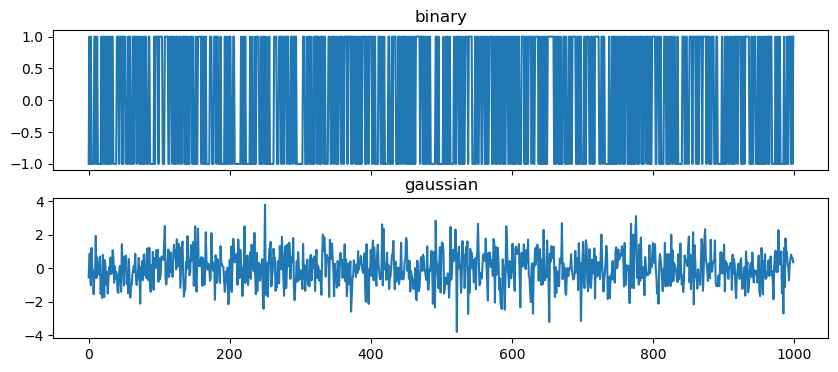
\includegraphics{resampling/FAQ_files/figure-pdf/cell-4-output-2.png}

}

\end{figure}

We see a marked dry season during the summer, so let's assume the
Hydrological Year ends in September.

\begin{Shaded}
\begin{Highlighting}[]
\NormalTok{df\_year }\OperatorTok{=}\NormalTok{ df.resample(}\StringTok{\textquotesingle{}A{-}SEP\textquotesingle{}}\NormalTok{).}\BuiltInTok{sum}\NormalTok{()}
\NormalTok{df\_year }\OperatorTok{=}\NormalTok{ df\_year.loc[}\StringTok{\textquotesingle{}1980\textquotesingle{}}\NormalTok{:}\StringTok{\textquotesingle{}2003\textquotesingle{}}\NormalTok{]}
\NormalTok{df\_year}
\end{Highlighting}
\end{Shaded}

\begin{verbatim}
/var/folders/c3/7hp0d36n6vv8jc9hm2440__00000gn/T/ipykernel_94063/2047090134.py:1: FutureWarning: The default value of numeric_only in DataFrameGroupBy.sum is deprecated. In a future version, numeric_only will default to False. Either specify numeric_only or select only columns which should be valid for the function.
  df_year = df.resample('A-SEP').sum()
\end{verbatim}

\begin{longtable}[]{@{}ll@{}}
\toprule\noalign{}
& rain \\
date & \\
\midrule\noalign{}
\endhead
\bottomrule\noalign{}
\endlastfoot
1980-09-30 & 355.5 \\
1981-09-30 & 463.1 \\
1982-09-30 & 221.7 \\
1983-09-30 & 557.1 \\
1984-09-30 & 335.3 \\
1985-09-30 & 379.8 \\
1986-09-30 & 300.7 \\
1987-09-30 & 424.7 \\
1988-09-30 & 421.6 \\
1989-09-30 & 251.6 \\
1990-09-30 & 432.5 \\
1991-09-30 & 328.3 \\
1992-09-30 & 738.4 \\
1993-09-30 & 434.9 \\
1994-09-30 & 255.4 \\
1995-09-30 & 408.6 \\
1996-09-30 & 373.0 \\
1997-09-30 & 416.2 \\
1998-09-30 & 451.9 \\
1999-09-30 & 227.8 \\
2000-09-30 & 378.9 \\
2001-09-30 & 273.9 \\
2002-09-30 & 445.2 \\
2003-09-30 & 602.4 \\
\end{longtable}

\begin{Shaded}
\begin{Highlighting}[]
\NormalTok{fig, ax }\OperatorTok{=}\NormalTok{ plt.subplots()}
\NormalTok{ax.bar(df\_year.index, df\_year[}\StringTok{\textquotesingle{}rain\textquotesingle{}}\NormalTok{], color}\OperatorTok{=}\StringTok{\textquotesingle{}black\textquotesingle{}}\NormalTok{,}
\NormalTok{       width}\OperatorTok{=}\DecValTok{365}\NormalTok{)}
\NormalTok{ax.set\_ylabel(}\StringTok{"yearly precipitation (mm)"}\NormalTok{)}
\NormalTok{ax.set\_title(}\StringTok{"Kvutzat Kinneret"}\NormalTok{)}
\end{Highlighting}
\end{Shaded}

\begin{verbatim}
Text(0.5, 1.0, 'Kvutzat Kinneret')
\end{verbatim}

\begin{figure}[H]

{\centering \includegraphics{resampling/FAQ_files/figure-pdf/cell-6-output-2.png}

}

\end{figure}

\hypertarget{when-upsampling-how-to-fill-missing-values-with-zero}{%
\section{When upsampling, how to fill missing values with
zero?}\label{when-upsampling-how-to-fill-missing-values-with-zero}}

We did that in the example above, like this:

\begin{Shaded}
\begin{Highlighting}[]
\NormalTok{df }\OperatorTok{=}\NormalTok{ df.resample(}\StringTok{\textquotesingle{}D\textquotesingle{}}\NormalTok{).asfreq().fillna(}\DecValTok{0}\NormalTok{)  }\CommentTok{\# asfreq = replace}
\end{Highlighting}
\end{Shaded}

\part{smoothing}

\hypertarget{motivation-1}{%
\chapter{motivation}\label{motivation-1}}

This is the temperature for the Yatir Forest (Shani station, see
\href{https://maps.app.goo.gl/JXfHcjE2Vn8YbS91A}{map}), between 2 and 5
of January 2022. Data is in intervals of 10 minutes, and was downloaded
from the Israel Meteorological Service.

\begin{Shaded}
\begin{Highlighting}[]
\ImportTok{import}\NormalTok{ numpy }\ImportTok{as}\NormalTok{ np}
\ImportTok{import}\NormalTok{ matplotlib.pyplot }\ImportTok{as}\NormalTok{ plt}
\ImportTok{import}\NormalTok{ pandas }\ImportTok{as}\NormalTok{ pd}
\ImportTok{from}\NormalTok{ matplotlib.dates }\ImportTok{import}\NormalTok{ DateFormatter}
\ImportTok{import}\NormalTok{ matplotlib.dates }\ImportTok{as}\NormalTok{ mdates}
\ImportTok{import}\NormalTok{ datetime }\ImportTok{as}\NormalTok{ dt}
\ImportTok{import}\NormalTok{ matplotlib.ticker }\ImportTok{as}\NormalTok{ ticker}
\ImportTok{import}\NormalTok{ warnings}
\CommentTok{\# Suppress FutureWarnings}
\NormalTok{warnings.simplefilter(action}\OperatorTok{=}\StringTok{\textquotesingle{}ignore\textquotesingle{}}\NormalTok{, category}\OperatorTok{=}\PreprocessorTok{FutureWarning}\NormalTok{)}
\ImportTok{import}\NormalTok{ seaborn }\ImportTok{as}\NormalTok{ sns}
\NormalTok{sns.}\BuiltInTok{set}\NormalTok{(style}\OperatorTok{=}\StringTok{"ticks"}\NormalTok{, font\_scale}\OperatorTok{=}\FloatTok{1.5}\NormalTok{)  }\CommentTok{\# white graphs, with large and legible letters}
\ImportTok{import}\NormalTok{ requests}
\ImportTok{import}\NormalTok{ json}
\ImportTok{import}\NormalTok{ os}
\CommentTok{\# \%matplotlib widget}
\end{Highlighting}
\end{Shaded}

\begin{Shaded}
\begin{Highlighting}[]
\CommentTok{\# read token from file}
\ControlFlowTok{with} \BuiltInTok{open}\NormalTok{(}\StringTok{\textquotesingle{}../archive/IMS{-}token.txt\textquotesingle{}}\NormalTok{, }\StringTok{\textquotesingle{}r\textquotesingle{}}\NormalTok{) }\ImportTok{as} \BuiltInTok{file}\NormalTok{:}
\NormalTok{    TOKEN }\OperatorTok{=} \BuiltInTok{file}\NormalTok{.readline()}
\CommentTok{\# 28 = SHANI station}
\NormalTok{STATION\_NUM }\OperatorTok{=} \DecValTok{28}
\NormalTok{start }\OperatorTok{=} \StringTok{"2022/01/01"}
\NormalTok{end }\OperatorTok{=} \StringTok{"2022/01/07"}
\NormalTok{filename }\OperatorTok{=} \StringTok{\textquotesingle{}shani\_2022\_january.json\textquotesingle{}}

\CommentTok{\# check if the JSON file already exists}
\CommentTok{\# if so, then load file}
\ControlFlowTok{if}\NormalTok{ os.path.exists(filename):}
    \ControlFlowTok{with} \BuiltInTok{open}\NormalTok{(filename, }\StringTok{\textquotesingle{}r\textquotesingle{}}\NormalTok{) }\ImportTok{as}\NormalTok{ json\_file:}
\NormalTok{        data }\OperatorTok{=}\NormalTok{ json.load(json\_file)}
\ControlFlowTok{else}\NormalTok{:}
    \CommentTok{\# make the API request if the file doesn\textquotesingle{}t exist}
\NormalTok{    url }\OperatorTok{=} \SpecialStringTok{f"https://api.ims.gov.il/v1/envista/stations/}\SpecialCharTok{\{}\NormalTok{STATION\_NUM}\SpecialCharTok{\}}\SpecialStringTok{/data/?from=}\SpecialCharTok{\{}\NormalTok{start}\SpecialCharTok{\}}\SpecialStringTok{\&to=}\SpecialCharTok{\{}\NormalTok{end}\SpecialCharTok{\}}\SpecialStringTok{"}
\NormalTok{    headers }\OperatorTok{=}\NormalTok{ \{}\StringTok{\textquotesingle{}Authorization\textquotesingle{}}\NormalTok{: }\SpecialStringTok{f\textquotesingle{}ApiToken }\SpecialCharTok{\{}\NormalTok{TOKEN}\SpecialCharTok{\}}\SpecialStringTok{\textquotesingle{}}\NormalTok{\}}
\NormalTok{    response }\OperatorTok{=}\NormalTok{ requests.get(url, headers}\OperatorTok{=}\NormalTok{headers)}
\NormalTok{    data }\OperatorTok{=}\NormalTok{ json.loads(response.text.encode(}\StringTok{\textquotesingle{}utf8\textquotesingle{}}\NormalTok{))}
    
    \CommentTok{\# save the JSON data to a file}
    \ControlFlowTok{with} \BuiltInTok{open}\NormalTok{(filename, }\StringTok{\textquotesingle{}w\textquotesingle{}}\NormalTok{) }\ImportTok{as}\NormalTok{ json\_file:}
\NormalTok{        json.dump(data, json\_file)}
\CommentTok{\# show data to see if it\textquotesingle{}s alright}
\CommentTok{\# data}
\end{Highlighting}
\end{Shaded}

\begin{Shaded}
\begin{Highlighting}[]
\NormalTok{df }\OperatorTok{=}\NormalTok{ pd.json\_normalize(data[}\StringTok{\textquotesingle{}data\textquotesingle{}}\NormalTok{],record\_path}\OperatorTok{=}\NormalTok{[}\StringTok{\textquotesingle{}channels\textquotesingle{}}\NormalTok{], meta}\OperatorTok{=}\NormalTok{[}\StringTok{\textquotesingle{}datetime\textquotesingle{}}\NormalTok{])}
\NormalTok{df[}\StringTok{\textquotesingle{}date\textquotesingle{}}\NormalTok{] }\OperatorTok{=}\NormalTok{ (pd.to\_datetime(df[}\StringTok{\textquotesingle{}datetime\textquotesingle{}}\NormalTok{])}
\NormalTok{                .dt.tz\_localize(}\VariableTok{None}\NormalTok{)  }\CommentTok{\# ignores time zone information}
\NormalTok{             )}
\NormalTok{df }\OperatorTok{=}\NormalTok{ df.pivot(index}\OperatorTok{=}\StringTok{\textquotesingle{}date\textquotesingle{}}\NormalTok{, columns}\OperatorTok{=}\StringTok{\textquotesingle{}name\textquotesingle{}}\NormalTok{, values}\OperatorTok{=}\StringTok{\textquotesingle{}value\textquotesingle{}}\NormalTok{)}
\CommentTok{\# df}
\end{Highlighting}
\end{Shaded}

\begin{Shaded}
\begin{Highlighting}[]
\CommentTok{\# dirty trick to have dates in the middle of the 24{-}hour period}
\CommentTok{\# make minor ticks in the middle, put the labels there!}
\CommentTok{\# from https://matplotlib.org/stable/gallery/ticks/centered\_ticklabels.html}

\KeywordTok{def}\NormalTok{ centered\_dates(ax):}
\NormalTok{    date\_form }\OperatorTok{=}\NormalTok{ DateFormatter(}\StringTok{"}\SpecialCharTok{\%d}\StringTok{ \%b"}\NormalTok{)  }\CommentTok{\# \%d 3{-}letter{-}Month}
    \CommentTok{\# major ticks at midnight, every day}
\NormalTok{    ax.xaxis.set\_major\_locator(mdates.DayLocator(interval}\OperatorTok{=}\DecValTok{1}\NormalTok{))}
\NormalTok{    ax.xaxis.set\_major\_formatter(date\_form)}
    \CommentTok{\# minor ticks at noon, every day}
\NormalTok{    ax.xaxis.set\_minor\_locator(mdates.HourLocator(byhour}\OperatorTok{=}\NormalTok{[}\DecValTok{12}\NormalTok{]))}
    \CommentTok{\# erase major tick labels}
\NormalTok{    ax.xaxis.set\_major\_formatter(ticker.NullFormatter())}
    \CommentTok{\# set minor tick labels as define above}
\NormalTok{    ax.xaxis.set\_minor\_formatter(date\_form)}
    \CommentTok{\# completely erase minor ticks, center tick labels}
    \ControlFlowTok{for}\NormalTok{ tick }\KeywordTok{in}\NormalTok{ ax.xaxis.get\_minor\_ticks():}
\NormalTok{        tick.tick1line.set\_markersize(}\DecValTok{0}\NormalTok{)}
\NormalTok{        tick.tick2line.set\_markersize(}\DecValTok{0}\NormalTok{)}
\NormalTok{        tick.label1.set\_horizontalalignment(}\StringTok{\textquotesingle{}center\textquotesingle{}}\NormalTok{)}
\end{Highlighting}
\end{Shaded}

\begin{Shaded}
\begin{Highlighting}[]
\NormalTok{fig, ax }\OperatorTok{=}\NormalTok{ plt.subplots(figsize}\OperatorTok{=}\NormalTok{(}\DecValTok{8}\NormalTok{,}\DecValTok{5}\NormalTok{))}
\NormalTok{start }\OperatorTok{=} \StringTok{"2022{-}01{-}02"}
\NormalTok{end }\OperatorTok{=} \StringTok{"2022{-}01{-}05"}
\NormalTok{df }\OperatorTok{=}\NormalTok{ df.loc[start:end]}
\NormalTok{ax.plot(df[}\StringTok{\textquotesingle{}TD\textquotesingle{}}\NormalTok{], color}\OperatorTok{=}\StringTok{\textquotesingle{}black\textquotesingle{}}\NormalTok{)}
\NormalTok{ax.}\BuiltInTok{set}\NormalTok{(ylim}\OperatorTok{=}\NormalTok{[}\DecValTok{5}\NormalTok{, }\FloatTok{17.5}\NormalTok{],}
\NormalTok{       xlim}\OperatorTok{=}\NormalTok{[df.index[}\DecValTok{0}\NormalTok{], df.index[}\OperatorTok{{-}}\DecValTok{1}\NormalTok{]],}
\NormalTok{       ylabel}\OperatorTok{=}\StringTok{"Temperature (°C)"}\NormalTok{,}
\NormalTok{       title}\OperatorTok{=}\StringTok{"Yatir Forest, 2022"}\NormalTok{,}
\NormalTok{       yticks}\OperatorTok{=}\NormalTok{[}\DecValTok{5}\NormalTok{,}\DecValTok{10}\NormalTok{,}\DecValTok{15}\NormalTok{])}
\NormalTok{centered\_dates(ax)}
\NormalTok{fig.savefig(}\StringTok{"YF{-}temperature\_2022\_jan.png"}\NormalTok{, dpi}\OperatorTok{=}\DecValTok{300}\NormalTok{)}
\end{Highlighting}
\end{Shaded}

\begin{figure}[H]

{\centering \includegraphics{smoothing/motivation_files/figure-pdf/cell-6-output-1.png}

}

\end{figure}

We see that the temperature curve has a rough profile. Can we find ways
of getting smoother curves?

We learned how to average over a window with \texttt{resample}. Let's
try that for a 2-hour window:

\begin{Shaded}
\begin{Highlighting}[]
\NormalTok{fig, ax }\OperatorTok{=}\NormalTok{ plt.subplots(figsize}\OperatorTok{=}\NormalTok{(}\DecValTok{8}\NormalTok{,}\DecValTok{5}\NormalTok{))}
\NormalTok{ax.plot(df[}\StringTok{\textquotesingle{}TD\textquotesingle{}}\NormalTok{], color}\OperatorTok{=}\StringTok{\textquotesingle{}black\textquotesingle{}}\NormalTok{)}
\NormalTok{ax.plot(df[}\StringTok{\textquotesingle{}TD\textquotesingle{}}\NormalTok{].resample(}\StringTok{\textquotesingle{}2H\textquotesingle{}}\NormalTok{).mean(),}
\NormalTok{        color}\OperatorTok{=}\StringTok{\textquotesingle{}xkcd:hot pink\textquotesingle{}}\NormalTok{, ls}\OperatorTok{=}\StringTok{\textquotesingle{}{-}\textquotesingle{}}\NormalTok{,}
\NormalTok{        marker}\OperatorTok{=}\StringTok{"o"}\NormalTok{, mfc}\OperatorTok{=}\StringTok{"None"}\NormalTok{)}
\NormalTok{ax.}\BuiltInTok{set}\NormalTok{(ylim}\OperatorTok{=}\NormalTok{[}\DecValTok{5}\NormalTok{, }\FloatTok{17.5}\NormalTok{],}
\NormalTok{       xlim}\OperatorTok{=}\NormalTok{[df.index[}\DecValTok{0}\NormalTok{], df.index[}\OperatorTok{{-}}\DecValTok{1}\NormalTok{]],}
\NormalTok{       ylabel}\OperatorTok{=}\StringTok{"Temperature (°C)"}\NormalTok{,}
\NormalTok{       title}\OperatorTok{=}\StringTok{"Yatir Forest, 2022"}\NormalTok{,}
\NormalTok{       yticks}\OperatorTok{=}\NormalTok{[}\DecValTok{5}\NormalTok{,}\DecValTok{10}\NormalTok{,}\DecValTok{15}\NormalTok{])}
\NormalTok{centered\_dates(ax)}
\end{Highlighting}
\end{Shaded}

\begin{figure}[H]

{\centering \includegraphics{smoothing/motivation_files/figure-pdf/cell-7-output-1.png}

}

\end{figure}

The temperature profile now is much smoother, but when using
\texttt{resample}, we lost temporal resolution. Our original data had
10-minute frequency, and now we have a 2-hour frequency.

How can we get a smoother curve without losing resolution?

\hypertarget{tumbling-vs-sliding}{%
\section{Tumbling vs Sliding}\label{tumbling-vs-sliding}}

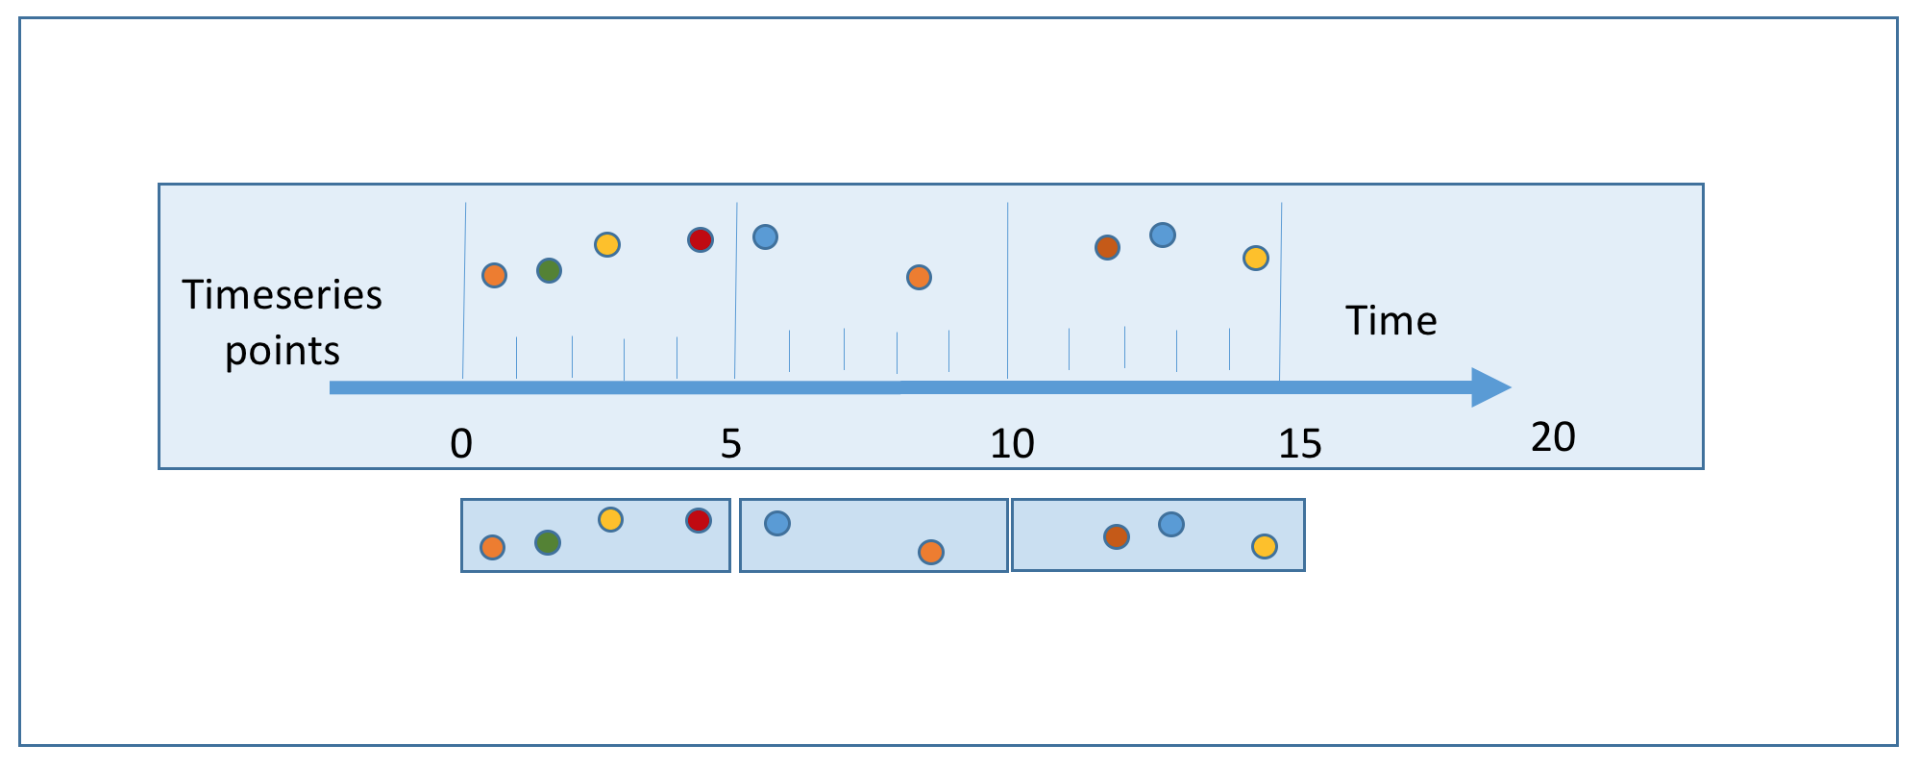
\includegraphics{smoothing/5sec_tumbling_window.png}
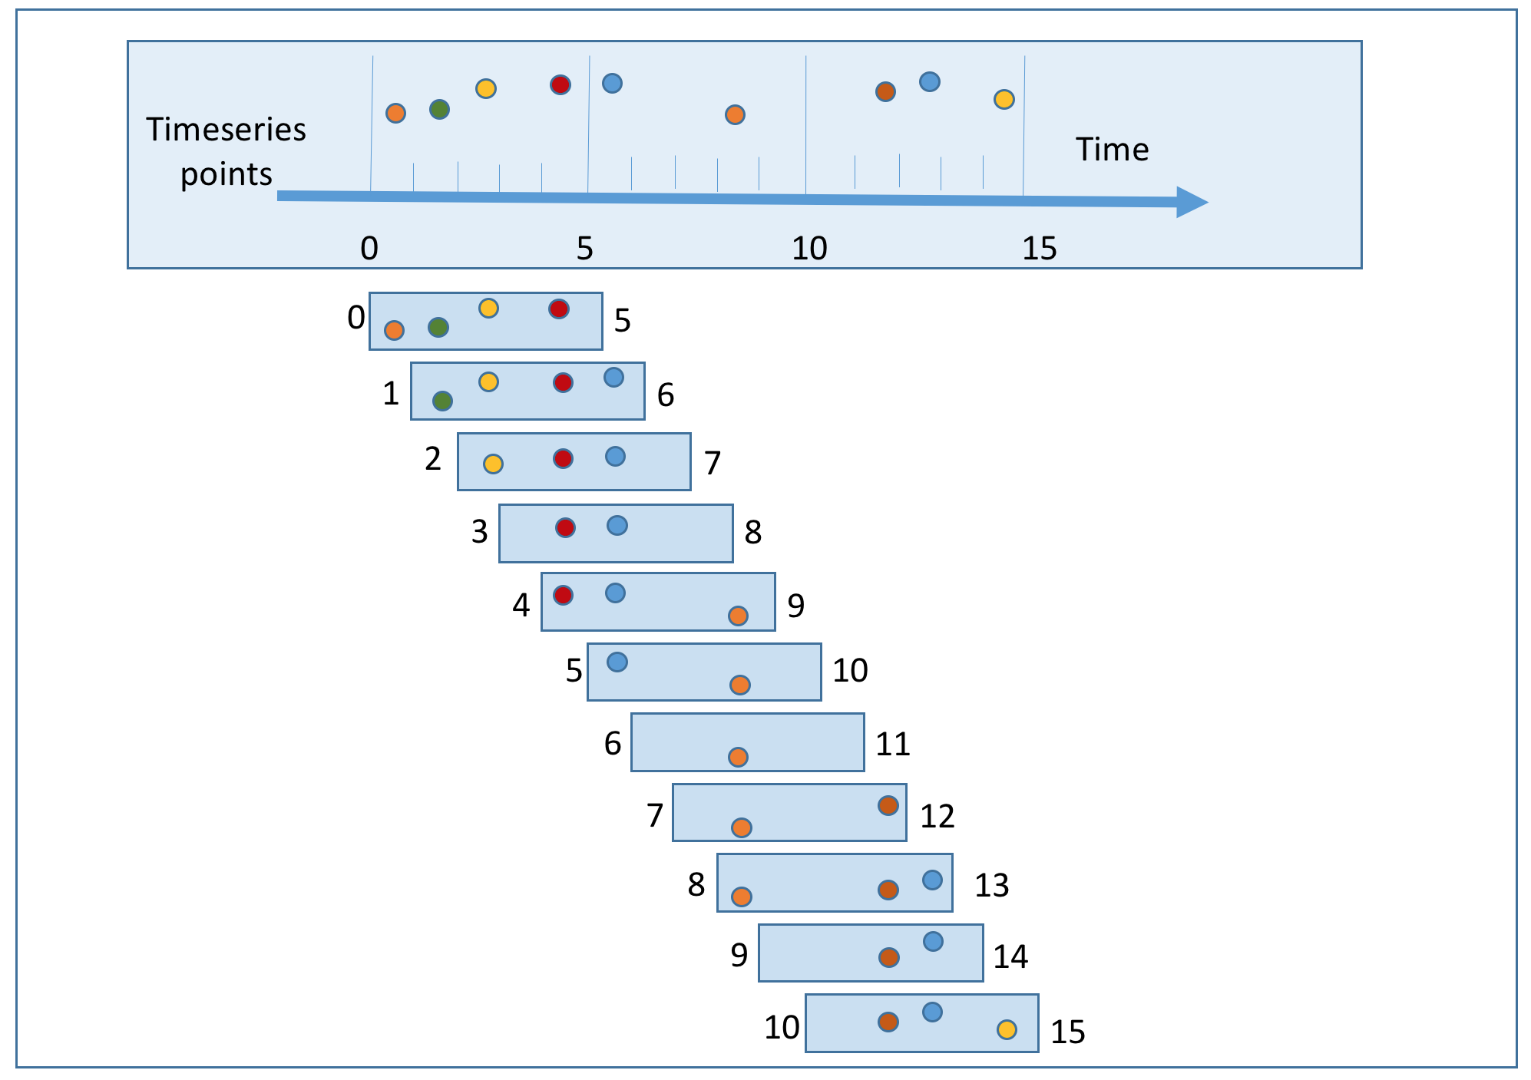
\includegraphics{smoothing/5sec_moving_window.png}

\hypertarget{sliding-window}{%
\chapter{sliding window}\label{sliding-window}}

This is the temperature for the Yatir Forest, between 2 and 5 of January
2022. Data (download .csv here) is in intervals of 10 minutes, and was
downloaded from the Israel Meteorological Service.

\begin{Shaded}
\begin{Highlighting}[]
\ImportTok{import}\NormalTok{ numpy }\ImportTok{as}\NormalTok{ np}
\ImportTok{import}\NormalTok{ matplotlib.pyplot }\ImportTok{as}\NormalTok{ plt}
\ImportTok{import}\NormalTok{ pandas }\ImportTok{as}\NormalTok{ pd}
\ImportTok{from}\NormalTok{ matplotlib.dates }\ImportTok{import}\NormalTok{ DateFormatter}
\ImportTok{import}\NormalTok{ matplotlib.dates }\ImportTok{as}\NormalTok{ mdates}
\ImportTok{import}\NormalTok{ datetime }\ImportTok{as}\NormalTok{ dt}
\ImportTok{import}\NormalTok{ matplotlib.ticker }\ImportTok{as}\NormalTok{ ticker}
\ImportTok{import}\NormalTok{ os}
\ImportTok{import}\NormalTok{ warnings}
\ImportTok{import}\NormalTok{ scipy}
\CommentTok{\# Suppress FutureWarnings}
\NormalTok{warnings.simplefilter(action}\OperatorTok{=}\StringTok{\textquotesingle{}ignore\textquotesingle{}}\NormalTok{, category}\OperatorTok{=}\PreprocessorTok{FutureWarning}\NormalTok{)}
\ImportTok{import}\NormalTok{ seaborn }\ImportTok{as}\NormalTok{ sns}
\NormalTok{sns.}\BuiltInTok{set}\NormalTok{(style}\OperatorTok{=}\StringTok{"ticks"}\NormalTok{, font\_scale}\OperatorTok{=}\FloatTok{1.5}\NormalTok{)  }\CommentTok{\# white graphs, with large and legible letters}
\CommentTok{\# \%matplotlib widget}
\end{Highlighting}
\end{Shaded}

\begin{Shaded}
\begin{Highlighting}[]
\CommentTok{\# dirty trick to have dates in the middle of the 24{-}hour period}
\CommentTok{\# make minor ticks in the middle, put the labels there!}
\CommentTok{\# from https://matplotlib.org/stable/gallery/ticks/centered\_ticklabels.html}

\KeywordTok{def}\NormalTok{ centered\_dates(ax):}
\NormalTok{    date\_form }\OperatorTok{=}\NormalTok{ DateFormatter(}\StringTok{"}\SpecialCharTok{\%d}\StringTok{ \%b"}\NormalTok{)  }\CommentTok{\# \%d 3{-}letter{-}Month}
    \CommentTok{\# major ticks at midnight, every day}
\NormalTok{    ax.xaxis.set\_major\_locator(mdates.DayLocator(interval}\OperatorTok{=}\DecValTok{1}\NormalTok{))}
\NormalTok{    ax.xaxis.set\_major\_formatter(date\_form)}
    \CommentTok{\# minor ticks at noon, every day}
\NormalTok{    ax.xaxis.set\_minor\_locator(mdates.HourLocator(byhour}\OperatorTok{=}\NormalTok{[}\DecValTok{12}\NormalTok{]))}
    \CommentTok{\# erase major tick labels}
\NormalTok{    ax.xaxis.set\_major\_formatter(ticker.NullFormatter())}
    \CommentTok{\# set minor tick labels as define above}
\NormalTok{    ax.xaxis.set\_minor\_formatter(date\_form)}
    \CommentTok{\# completely erase minor ticks, center tick labels}
    \ControlFlowTok{for}\NormalTok{ tick }\KeywordTok{in}\NormalTok{ ax.xaxis.get\_minor\_ticks():}
\NormalTok{        tick.tick1line.set\_markersize(}\DecValTok{0}\NormalTok{)}
\NormalTok{        tick.tick2line.set\_markersize(}\DecValTok{0}\NormalTok{)}
\NormalTok{        tick.label1.set\_horizontalalignment(}\StringTok{\textquotesingle{}center\textquotesingle{}}\NormalTok{)}
\end{Highlighting}
\end{Shaded}

\begin{Shaded}
\begin{Highlighting}[]
\NormalTok{df }\OperatorTok{=}\NormalTok{ pd.read\_csv(}\StringTok{\textquotesingle{}shani\_2022\_january.csv\textquotesingle{}}\NormalTok{, parse\_dates}\OperatorTok{=}\NormalTok{[}\StringTok{\textquotesingle{}date\textquotesingle{}}\NormalTok{], index\_col}\OperatorTok{=}\StringTok{\textquotesingle{}date\textquotesingle{}}\NormalTok{)}
\end{Highlighting}
\end{Shaded}

\begin{Shaded}
\begin{Highlighting}[]
\NormalTok{fig, ax }\OperatorTok{=}\NormalTok{ plt.subplots(figsize}\OperatorTok{=}\NormalTok{(}\DecValTok{8}\NormalTok{,}\DecValTok{5}\NormalTok{))}
\NormalTok{start }\OperatorTok{=} \StringTok{"2022{-}01{-}02"}
\NormalTok{end }\OperatorTok{=} \StringTok{"2022{-}01{-}05"}
\NormalTok{df }\OperatorTok{=}\NormalTok{ df.loc[start:end]}
\NormalTok{ax.plot(df[}\StringTok{\textquotesingle{}TD\textquotesingle{}}\NormalTok{], color}\OperatorTok{=}\StringTok{\textquotesingle{}black\textquotesingle{}}\NormalTok{)}

\NormalTok{plot\_settings }\OperatorTok{=}\NormalTok{ \{}
    \StringTok{\textquotesingle{}ylim\textquotesingle{}}\NormalTok{: [}\DecValTok{5}\NormalTok{, }\FloatTok{17.5}\NormalTok{],}
    \StringTok{\textquotesingle{}xlim\textquotesingle{}}\NormalTok{: [df.index[}\DecValTok{0}\NormalTok{], df.index[}\OperatorTok{{-}}\DecValTok{1}\NormalTok{]],}
    \StringTok{\textquotesingle{}ylabel\textquotesingle{}}\NormalTok{: }\StringTok{"Temperature (°C)"}\NormalTok{,}
    \StringTok{\textquotesingle{}title\textquotesingle{}}\NormalTok{: }\StringTok{"Yatir Forest, 2022"}\NormalTok{,}
    \StringTok{\textquotesingle{}yticks\textquotesingle{}}\NormalTok{: [}\DecValTok{5}\NormalTok{, }\DecValTok{10}\NormalTok{, }\DecValTok{15}\NormalTok{]}
\NormalTok{\}}

\NormalTok{ax.}\BuiltInTok{set}\NormalTok{(}\OperatorTok{**}\NormalTok{plot\_settings)}
\NormalTok{centered\_dates(ax)}
\end{Highlighting}
\end{Shaded}

\begin{figure}[H]

{\centering \includegraphics{smoothing/sliding_files/figure-pdf/cell-5-output-1.png}

}

\end{figure}

We see that the temperature curve has a rough profile. Can we find ways
of getting smoother curves?

\hypertarget{convolution}{%
\section{convolution}\label{convolution}}

Convolution is a fancy word for averaging a time series using a sliding
window. We will use the terms \textbf{convolution, running average, and
rolling average} interchangeably. See the animation below. We take all
temperature values inside a window of width 500 minutes (51 points), and
average them with equal weights. The weights profile is called
\texttt{kernel}.

The pink curve is much smoother than the original! However, the running
average cannot describe sharp temperature changes. If we decrease the
window width to 200 minutes (21 points), we get the following result.

There is a tradeoff between the smoothness of a curve, and its ability
to describe sharp temporal changes.

\hypertarget{kernels}{%
\section{kernels}\label{kernels}}

We can modify our running average, so that values closer to the center
of the window have higher weights, and those further away count less.
This is achieved by changing the weight profile, or the shape of the
kernel. We see below the result of a running average using a triangular
window of base 500 minutes (51 points).

Things can get as fancy as we want. Instead of a triangular kernel,
which has sharp edges, we can choose a smoother gaussian kernel, see the
difference below. We used a gaussian kernel with 60-minute standard
deviation.

See how the three kernel shapes compare. There are
\href{https://docs.scipy.org/doc/scipy/reference/signal.windows.html\#module-scipy.signal.windows}{\emph{many}
kernels to chose from}. 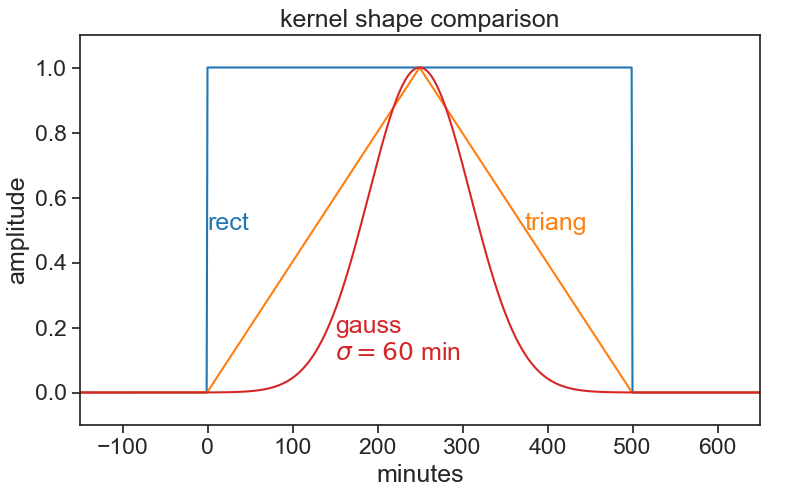
\includegraphics{smoothing/kernel_shapes.png}

\hypertarget{math}{%
\section{math}\label{math}}

The definition of a convolution between signal \(f(t)\) and kernel
\(k(t)\) is

\[
(f * k)(t) = \int f(\tau)k(t-\tau)d\tau.
\]

The expression \(f*k\) denotes the convolution of these two functions.
The argument of \(k\) is \(t-\tau\), meaning that the kernel runs from
left to right (as \(t\) does), and at every point the two signals (\(f\)
and \(k\)) are multiplied together. It is the product of the signal with
the weight function \(k\) that gives us an average. Because of
\(-\tau\), the kernel is flipped backwards, but this has no effect to
symmetric kernels, like to ones in the examples above. Finally, the
actual running average is not the convolution, but

\[
\frac{(f * k)(t)}{\displaystyle \int k(t)dt}.
\]

Whenever the integral of the kernel is 1, then the convolution will be
identical with the running average.

\hypertarget{numerics}{%
\section{numerics}\label{numerics}}

Running averages are very common tools in time-series analysis. The
\texttt{pandas} package makes life quite simple. For example, in order
to calculate the running average of temperature using a rectangular
kernel, one writes:

\begin{Shaded}
\begin{Highlighting}[]
\NormalTok{df[}\StringTok{\textquotesingle{}temp\_smoothed\textquotesingle{}}\NormalTok{] }\OperatorTok{=}\NormalTok{ (}
\NormalTok{                       df[}\StringTok{\textquotesingle{}TD\textquotesingle{}}\NormalTok{].rolling(window}\OperatorTok{=}\StringTok{\textquotesingle{}500min\textquotesingle{}}\NormalTok{,}
\NormalTok{                                        min\_periods}\OperatorTok{=}\DecValTok{50}   \CommentTok{\# comment this to see what happens}
\NormalTok{                                        )}
\NormalTok{                               .mean()}
\NormalTok{                      )}

\NormalTok{fig, ax }\OperatorTok{=}\NormalTok{ plt.subplots(figsize}\OperatorTok{=}\NormalTok{(}\DecValTok{8}\NormalTok{,}\DecValTok{5}\NormalTok{))}
\NormalTok{ax.plot(df[}\StringTok{\textquotesingle{}TD\textquotesingle{}}\NormalTok{], color}\OperatorTok{=}\StringTok{\textquotesingle{}black\textquotesingle{}}\NormalTok{)}
\NormalTok{ax.plot(df[}\StringTok{\textquotesingle{}temp\_smoothed\textquotesingle{}}\NormalTok{], color}\OperatorTok{=}\StringTok{\textquotesingle{}xkcd:hot pink\textquotesingle{}}\NormalTok{)}
\NormalTok{ax.}\BuiltInTok{set}\NormalTok{(}\OperatorTok{**}\NormalTok{plot\_settings)}
\NormalTok{centered\_dates(ax)}
\end{Highlighting}
\end{Shaded}

\begin{figure}[H]

{\centering \includegraphics{smoothing/sliding_files/figure-pdf/cell-6-output-1.png}

}

\end{figure}

The pink curve looks smooth, but why does it lag behind the data?!
What's going on?

\hypertarget{day-average-of-covid-19-infections}{%
\subsection{7-day average of COVID-19
infections}\label{day-average-of-covid-19-infections}}

During the COVID-19 pandemic, we would see graphs like this all the time
in the news:

\begin{Shaded}
\begin{Highlighting}[]
\CommentTok{\# data from https://health.google.com/covid{-}19/open{-}data/raw{-}data?loc=IL}
\CommentTok{\# define the local file path}
\NormalTok{local\_file\_path }\OperatorTok{=} \StringTok{\textquotesingle{}COVID\_19\_israel.csv\textquotesingle{}}
\CommentTok{\# check if the local file exists}
\ControlFlowTok{if}\NormalTok{ os.path.exists(local\_file\_path):}
    \CommentTok{\# if the local file exists, load it}
\NormalTok{    covid\_IL }\OperatorTok{=}\NormalTok{ pd.read\_csv(local\_file\_path, parse\_dates}\OperatorTok{=}\NormalTok{[}\StringTok{\textquotesingle{}date\textquotesingle{}}\NormalTok{], index\_col}\OperatorTok{=}\StringTok{\textquotesingle{}date\textquotesingle{}}\NormalTok{)}
\ControlFlowTok{else}\NormalTok{:}
    \CommentTok{\# if the local file doesn\textquotesingle{}t exist, download from the URL}
\NormalTok{    url }\OperatorTok{=} \StringTok{"https://storage.googleapis.com/covid19{-}open{-}data/v3/location/IL.csv"}
\NormalTok{    covid\_IL }\OperatorTok{=}\NormalTok{ pd.read\_csv(url, parse\_dates}\OperatorTok{=}\NormalTok{[}\StringTok{\textquotesingle{}date\textquotesingle{}}\NormalTok{], index\_col}\OperatorTok{=}\StringTok{\textquotesingle{}date\textquotesingle{}}\NormalTok{)}
    \CommentTok{\# save the downloaded data to the local file for future use}
\NormalTok{    covid\_IL.to\_csv(local\_file\_path)}

\NormalTok{df\_covid }\OperatorTok{=}\NormalTok{ covid\_IL[}\StringTok{\textquotesingle{}new\_confirmed\textquotesingle{}}\NormalTok{].to\_frame()}
\NormalTok{df\_covid[}\StringTok{\textquotesingle{}7d\_avg\textquotesingle{}}\NormalTok{] }\OperatorTok{=}\NormalTok{ df\_covid[}\StringTok{\textquotesingle{}new\_confirmed\textquotesingle{}}\NormalTok{].rolling(window}\OperatorTok{=}\StringTok{\textquotesingle{}7D\textquotesingle{}}\NormalTok{).mean()}
\end{Highlighting}
\end{Shaded}

\begin{Shaded}
\begin{Highlighting}[]
\NormalTok{fig, ax }\OperatorTok{=}\NormalTok{ plt.subplots(figsize}\OperatorTok{=}\NormalTok{(}\DecValTok{8}\NormalTok{,}\DecValTok{5}\NormalTok{))}
\NormalTok{st }\OperatorTok{=} \StringTok{\textquotesingle{}2022{-}01{-}01\textquotesingle{}}
\NormalTok{en }\OperatorTok{=} \StringTok{\textquotesingle{}2022{-}03{-}30\textquotesingle{}}
\NormalTok{new\_cases }\OperatorTok{=}\NormalTok{ ax.bar(df\_covid[st:en].index, df\_covid.loc[st:en,}\StringTok{\textquotesingle{}new\_confirmed\textquotesingle{}}\NormalTok{],}
\NormalTok{       color}\OperatorTok{=}\StringTok{"tab:blue"}\NormalTok{, width}\OperatorTok{=}\DecValTok{1}\NormalTok{)}
\NormalTok{mov\_avg, }\OperatorTok{=}\NormalTok{ ax.plot(df\_covid.loc[st:en,}\StringTok{\textquotesingle{}7d\_avg\textquotesingle{}}\NormalTok{],}
\NormalTok{        color}\OperatorTok{=}\StringTok{\textquotesingle{}xkcd:hot pink\textquotesingle{}}\NormalTok{)}
\NormalTok{ax.legend(handles}\OperatorTok{=}\NormalTok{[new\_cases, mov\_avg],}
\NormalTok{          labels}\OperatorTok{=}\NormalTok{[}\StringTok{\textquotesingle{}new confirmed cases\textquotesingle{}}\NormalTok{, }\StringTok{\textquotesingle{}7{-}day moving average\textquotesingle{}}\NormalTok{],}
\NormalTok{          frameon}\OperatorTok{=}\VariableTok{False}\NormalTok{)}
\NormalTok{weird\_day }\OperatorTok{=} \StringTok{"2022{-}02{-}12"}
\NormalTok{weird\_day\_x }\OperatorTok{=}\NormalTok{ mdates.date2num(dt.datetime.strptime(weird\_day, }\StringTok{"\%Y{-}\%m{-}}\SpecialCharTok{\%d}\StringTok{"}\NormalTok{))}
\NormalTok{ax.text(weird\_day\_x, df\_covid.loc[weird\_day,}\StringTok{\textquotesingle{}new\_confirmed\textquotesingle{}}\NormalTok{], }\StringTok{"?"}\NormalTok{)}
\CommentTok{\# formating dates on x axis}
\NormalTok{locator }\OperatorTok{=}\NormalTok{ mdates.AutoDateLocator(minticks}\OperatorTok{=}\DecValTok{7}\NormalTok{, maxticks}\OperatorTok{=}\DecValTok{11}\NormalTok{)}
\NormalTok{formatter }\OperatorTok{=}\NormalTok{ mdates.ConciseDateFormatter(locator)}
\NormalTok{ax.xaxis.set\_major\_locator(locator)}
\NormalTok{ax.xaxis.set\_major\_formatter(formatter)}
\end{Highlighting}
\end{Shaded}

\begin{figure}[H]

{\centering 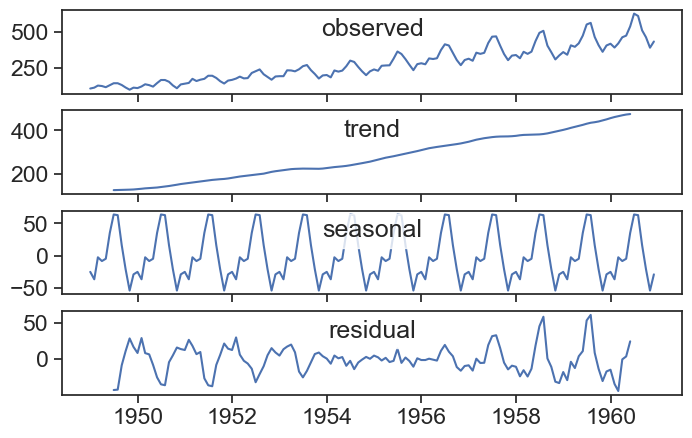
\includegraphics{smoothing/sliding_files/figure-pdf/cell-8-output-1.png}

}

\end{figure}

Take a look at the moving average next to the question mark. How can it
be that high, when all the bars around that date are lower? Is the
calculation right?

The answer is that the result of the moving average is assigned to the
right-most date in the running window. This is reasonable for COVID-19
cases: for a given day, I can only calculate a 7-day average based on
\textbf{past} values, I don't know what the future will be.

There is a simple way of assigning the result to the center of the
window:

\begin{Shaded}
\begin{Highlighting}[]
\NormalTok{df\_covid[}\StringTok{\textquotesingle{}7d\_avg\_center\textquotesingle{}}\NormalTok{] }\OperatorTok{=}\NormalTok{ (}
\NormalTok{                             df\_covid[}\StringTok{\textquotesingle{}new\_confirmed\textquotesingle{}}\NormalTok{]}
\NormalTok{                                 .rolling(window}\OperatorTok{=}\StringTok{\textquotesingle{}7D\textquotesingle{}}\NormalTok{,}
\NormalTok{                                          center}\OperatorTok{=}\VariableTok{True}\NormalTok{)  }\CommentTok{\# THIS}
\NormalTok{                                 .mean()}
\NormalTok{                            )}
\end{Highlighting}
\end{Shaded}

\begin{Shaded}
\begin{Highlighting}[]
\NormalTok{fig, ax }\OperatorTok{=}\NormalTok{ plt.subplots(figsize}\OperatorTok{=}\NormalTok{(}\DecValTok{8}\NormalTok{,}\DecValTok{5}\NormalTok{))}
\NormalTok{st }\OperatorTok{=} \StringTok{\textquotesingle{}2022{-}01{-}01\textquotesingle{}}
\NormalTok{en }\OperatorTok{=} \StringTok{\textquotesingle{}2022{-}03{-}30\textquotesingle{}}
\NormalTok{new\_cases }\OperatorTok{=}\NormalTok{ ax.bar(df\_covid[st:en].index, df\_covid.loc[st:en,}\StringTok{\textquotesingle{}new\_confirmed\textquotesingle{}}\NormalTok{],}
\NormalTok{       color}\OperatorTok{=}\StringTok{"tab:blue"}\NormalTok{, width}\OperatorTok{=}\DecValTok{1}\NormalTok{)}
\NormalTok{mov\_avg, }\OperatorTok{=}\NormalTok{ ax.plot(df\_covid.loc[st:en,}\StringTok{\textquotesingle{}7d\_avg\textquotesingle{}}\NormalTok{],}
\NormalTok{        color}\OperatorTok{=}\StringTok{\textquotesingle{}xkcd:hot pink\textquotesingle{}}\NormalTok{)}
\NormalTok{mov\_avg\_center, }\OperatorTok{=}\NormalTok{ ax.plot(df\_covid.loc[st:en,}\StringTok{\textquotesingle{}7d\_avg\_center\textquotesingle{}}\NormalTok{],}
\NormalTok{                          color}\OperatorTok{=}\StringTok{\textquotesingle{}xkcd:mustard\textquotesingle{}}\NormalTok{)}
\NormalTok{ax.legend(handles}\OperatorTok{=}\NormalTok{[new\_cases, mov\_avg, mov\_avg\_center],}
\NormalTok{          labels}\OperatorTok{=}\NormalTok{[}\StringTok{\textquotesingle{}new confirmed cases\textquotesingle{}}\NormalTok{,}
                  \StringTok{\textquotesingle{}7{-}day moving average\textquotesingle{}}\NormalTok{,}
                  \StringTok{\textquotesingle{}CENTERED 7{-}day}\CharTok{\textbackslash{}n}\StringTok{moving average\textquotesingle{}}\NormalTok{],}
\NormalTok{          frameon}\OperatorTok{=}\VariableTok{False}\NormalTok{)}
\CommentTok{\# formating dates on x axis}
\NormalTok{locator }\OperatorTok{=}\NormalTok{ mdates.AutoDateLocator(minticks}\OperatorTok{=}\DecValTok{7}\NormalTok{, maxticks}\OperatorTok{=}\DecValTok{11}\NormalTok{)}
\NormalTok{formatter }\OperatorTok{=}\NormalTok{ mdates.ConciseDateFormatter(locator)}
\NormalTok{ax.xaxis.set\_major\_locator(locator)}
\NormalTok{ax.xaxis.set\_major\_formatter(formatter)}
\end{Highlighting}
\end{Shaded}

\begin{figure}[H]

{\centering \includegraphics{smoothing/sliding_files/figure-pdf/cell-10-output-1.png}

}

\end{figure}

As a rule, we will used a \textbf{centered} moving average
(\texttt{center=True}), unless stated otherwise. Also, only use
\texttt{min\_periods} if you know what you are doing.

\hypertarget{gaussian}{%
\subsection{gaussian}\label{gaussian}}

You can easily change the kernel shape by using the \texttt{win\_type}
argument. See how to perform a rolling mean with a gaussian kernel:

\begin{Shaded}
\begin{Highlighting}[]
\NormalTok{(}
\NormalTok{df[}\StringTok{\textquotesingle{}temperature\textquotesingle{}}\NormalTok{].rolling(window}\OperatorTok{=}\NormalTok{window\_width,}
\NormalTok{                          center}\OperatorTok{=}\VariableTok{True}\NormalTok{,}
\NormalTok{                          win\_type}\OperatorTok{=}\StringTok{"gaussian"}\NormalTok{)}
\NormalTok{                 .mean(std}\OperatorTok{=}\NormalTok{std\_gaussian)}
\NormalTok{)}
\end{Highlighting}
\end{Shaded}

where

\begin{itemize}
\tightlist
\item
  \texttt{window\_width} is an integer, number of points in your window
\item
  \texttt{std\_gaussian} is the standard deviation of your gaussian,
  \textbf{measured in sample points, not time!}
\end{itemize}

For instance, if we have measurements every 10 minutes, and our window
width is 500 minutes, then \texttt{window\_width\ =\ 500/10\ +\ 1}
(first and last included). If we want a standard deviation of 60
minutes, then \texttt{std\_gaussian\ =\ 6}. The gaussian kernel will
look like this:

\begin{Shaded}
\begin{Highlighting}[]
\NormalTok{window\_width }\OperatorTok{=} \DecValTok{50}  \CommentTok{\# in points = 500 min}
\NormalTok{std }\OperatorTok{=} \DecValTok{6}  \CommentTok{\# in points = 60 min}
\NormalTok{fig, ax }\OperatorTok{=}\NormalTok{ plt.subplots(figsize}\OperatorTok{=}\NormalTok{(}\DecValTok{8}\NormalTok{,}\DecValTok{5}\NormalTok{))}
\NormalTok{g }\OperatorTok{=}\NormalTok{ scipy.signal.gaussian(window\_width, std)}
\NormalTok{ax.plot(g)}
\NormalTok{ax.}\BuiltInTok{set}\NormalTok{(xlabel}\OperatorTok{=}\StringTok{"window width (points)"}\NormalTok{,}
\NormalTok{       ylabel}\OperatorTok{=}\StringTok{"kernel weights"}\NormalTok{,}
\NormalTok{       title}\OperatorTok{=}\StringTok{"gaussian kernel"}\NormalTok{)}\OperatorTok{;}
\end{Highlighting}
\end{Shaded}

\begin{figure}[H]

{\centering \includegraphics{smoothing/sliding_files/figure-pdf/cell-11-output-1.png}

}

\end{figure}

You can take a look at various options for kernel shapes
\href{https://docs.scipy.org/doc/scipy/reference/signal.windows.html\#module-scipy.signal.windows}{here},
provided by the \texttt{scipy} package.

\hypertarget{triangular}{%
\subsection{triangular}\label{triangular}}

Same idea as gaussian, but simpler, because we don't need to think about
standard deviation.

\begin{Shaded}
\begin{Highlighting}[]
\NormalTok{(}
\NormalTok{df[}\StringTok{\textquotesingle{}temperature\textquotesingle{}}\NormalTok{].rolling(window}\OperatorTok{=}\NormalTok{window\_width,}
\NormalTok{                          center}\OperatorTok{=}\VariableTok{True}\NormalTok{,}
\NormalTok{                          win\_type}\OperatorTok{=}\StringTok{"triang"}\NormalTok{)}
\NormalTok{                 .mean()}
\NormalTok{)}
\end{Highlighting}
\end{Shaded}

\hypertarget{which-window-shape-and-width-to-choose}{%
\section{which window shape and width to
choose?}\label{which-window-shape-and-width-to-choose}}

🤷‍♂️

Sorry, there is not definite answer here\ldots{} It really depends on
your data and what you need to do with it. See below a comparison of all
examples in the videos above.

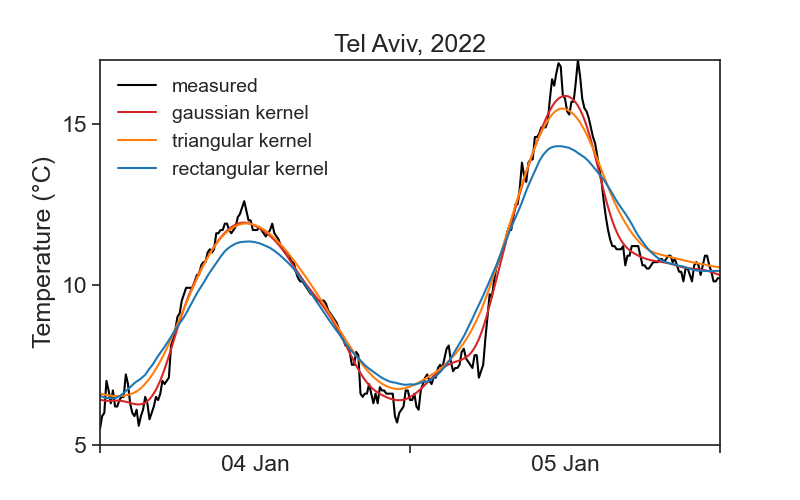
\includegraphics{smoothing/kernel_comparison.png}

One important question you need to ask is: what are the time scales
associated with the processes I'm interested in? For example, if I'm
interested in the daily temperature pattern, getting rid of
1-minute-long fluctuations would probably be ok. On the other hand, if
we were to smooth the signal so much that all that can be seen are the
temperature changes between summer and winter, then my smoothing got out
of hand, and I threw away the very process I wanted to study.

All this is to say that you need to know in advance a few things about
the system you are studying, otherwise you can't know what is ``noise''
that can be smoothed away.

\hypertarget{not-only-averages}{%
\chapter{not only averages}\label{not-only-averages}}

\begin{Shaded}
\begin{Highlighting}[]
\ImportTok{import}\NormalTok{ numpy }\ImportTok{as}\NormalTok{ np}
\ImportTok{import}\NormalTok{ matplotlib.pyplot }\ImportTok{as}\NormalTok{ plt}
\ImportTok{import}\NormalTok{ pandas }\ImportTok{as}\NormalTok{ pd}
\ImportTok{from}\NormalTok{ matplotlib.dates }\ImportTok{import}\NormalTok{ DateFormatter}
\ImportTok{import}\NormalTok{ matplotlib.dates }\ImportTok{as}\NormalTok{ mdates}
\ImportTok{import}\NormalTok{ datetime }\ImportTok{as}\NormalTok{ dt}
\ImportTok{import}\NormalTok{ matplotlib.ticker }\ImportTok{as}\NormalTok{ ticker}
\ImportTok{import}\NormalTok{ warnings}
\CommentTok{\# Suppress FutureWarnings}
\NormalTok{warnings.simplefilter(action}\OperatorTok{=}\StringTok{\textquotesingle{}ignore\textquotesingle{}}\NormalTok{, category}\OperatorTok{=}\PreprocessorTok{FutureWarning}\NormalTok{)}
\ImportTok{import}\NormalTok{ seaborn }\ImportTok{as}\NormalTok{ sns}
\NormalTok{sns.}\BuiltInTok{set}\NormalTok{(style}\OperatorTok{=}\StringTok{"ticks"}\NormalTok{, font\_scale}\OperatorTok{=}\FloatTok{1.5}\NormalTok{)  }\CommentTok{\# white graphs, with large and legible letters}
\ImportTok{import}\NormalTok{ requests}
\ImportTok{import}\NormalTok{ json}
\ImportTok{import}\NormalTok{ os}
\CommentTok{\# \%matplotlib widget}
\end{Highlighting}
\end{Shaded}

\begin{Shaded}
\begin{Highlighting}[]
\CommentTok{\# read token from file}
\ControlFlowTok{with} \BuiltInTok{open}\NormalTok{(}\StringTok{\textquotesingle{}../archive/IMS{-}token.txt\textquotesingle{}}\NormalTok{, }\StringTok{\textquotesingle{}r\textquotesingle{}}\NormalTok{) }\ImportTok{as} \BuiltInTok{file}\NormalTok{:}
\NormalTok{    TOKEN }\OperatorTok{=} \BuiltInTok{file}\NormalTok{.readline()}
\CommentTok{\# 28 = SHANI station}
\NormalTok{STATION\_NUM }\OperatorTok{=} \DecValTok{28}
\NormalTok{start }\OperatorTok{=} \StringTok{"2022/01/01"}
\NormalTok{end }\OperatorTok{=} \StringTok{"2022/01/07"}
\NormalTok{filename }\OperatorTok{=} \StringTok{\textquotesingle{}shani\_2022\_january.json\textquotesingle{}}

\CommentTok{\# check if the JSON file already exists}
\CommentTok{\# if so, then load file}
\ControlFlowTok{if}\NormalTok{ os.path.exists(filename):}
    \ControlFlowTok{with} \BuiltInTok{open}\NormalTok{(filename, }\StringTok{\textquotesingle{}r\textquotesingle{}}\NormalTok{) }\ImportTok{as}\NormalTok{ json\_file:}
\NormalTok{        data }\OperatorTok{=}\NormalTok{ json.load(json\_file)}
\ControlFlowTok{else}\NormalTok{:}
    \CommentTok{\# make the API request if the file doesn\textquotesingle{}t exist}
\NormalTok{    url }\OperatorTok{=} \SpecialStringTok{f"https://api.ims.gov.il/v1/envista/stations/}\SpecialCharTok{\{}\NormalTok{STATION\_NUM}\SpecialCharTok{\}}\SpecialStringTok{/data/?from=}\SpecialCharTok{\{}\NormalTok{start}\SpecialCharTok{\}}\SpecialStringTok{\&to=}\SpecialCharTok{\{}\NormalTok{end}\SpecialCharTok{\}}\SpecialStringTok{"}
\NormalTok{    headers }\OperatorTok{=}\NormalTok{ \{}\StringTok{\textquotesingle{}Authorization\textquotesingle{}}\NormalTok{: }\SpecialStringTok{f\textquotesingle{}ApiToken }\SpecialCharTok{\{}\NormalTok{TOKEN}\SpecialCharTok{\}}\SpecialStringTok{\textquotesingle{}}\NormalTok{\}}
\NormalTok{    response }\OperatorTok{=}\NormalTok{ requests.get(url, headers}\OperatorTok{=}\NormalTok{headers)}
\NormalTok{    data }\OperatorTok{=}\NormalTok{ json.loads(response.text.encode(}\StringTok{\textquotesingle{}utf8\textquotesingle{}}\NormalTok{))}
    
    \CommentTok{\# save the JSON data to a file}
    \ControlFlowTok{with} \BuiltInTok{open}\NormalTok{(filename, }\StringTok{\textquotesingle{}w\textquotesingle{}}\NormalTok{) }\ImportTok{as}\NormalTok{ json\_file:}
\NormalTok{        json.dump(data, json\_file)}
\CommentTok{\# show data to see if it\textquotesingle{}s alright}
\CommentTok{\# data}
\end{Highlighting}
\end{Shaded}

\begin{Shaded}
\begin{Highlighting}[]
\NormalTok{df }\OperatorTok{=}\NormalTok{ pd.json\_normalize(data[}\StringTok{\textquotesingle{}data\textquotesingle{}}\NormalTok{],record\_path}\OperatorTok{=}\NormalTok{[}\StringTok{\textquotesingle{}channels\textquotesingle{}}\NormalTok{], meta}\OperatorTok{=}\NormalTok{[}\StringTok{\textquotesingle{}datetime\textquotesingle{}}\NormalTok{])}
\NormalTok{df[}\StringTok{\textquotesingle{}date\textquotesingle{}}\NormalTok{] }\OperatorTok{=}\NormalTok{ (pd.to\_datetime(df[}\StringTok{\textquotesingle{}datetime\textquotesingle{}}\NormalTok{])}
\NormalTok{                .dt.tz\_localize(}\VariableTok{None}\NormalTok{)  }\CommentTok{\# ignores time zone information}
\NormalTok{             )}
\NormalTok{df }\OperatorTok{=}\NormalTok{ df.pivot(index}\OperatorTok{=}\StringTok{\textquotesingle{}date\textquotesingle{}}\NormalTok{, columns}\OperatorTok{=}\StringTok{\textquotesingle{}name\textquotesingle{}}\NormalTok{, values}\OperatorTok{=}\StringTok{\textquotesingle{}value\textquotesingle{}}\NormalTok{)}
\CommentTok{\# let\textquotesingle{}s work only with a few days, and only temperature}
\NormalTok{start }\OperatorTok{=} \StringTok{"2022{-}01{-}02"}
\NormalTok{end }\OperatorTok{=} \StringTok{"2022{-}01{-}05"}
\NormalTok{df }\OperatorTok{=}\NormalTok{ df.loc[start:end, }\StringTok{\textquotesingle{}TD\textquotesingle{}}\NormalTok{].to\_frame()}
\NormalTok{df.rename(columns}\OperatorTok{=}\NormalTok{\{}\StringTok{"TD"}\NormalTok{: }\StringTok{"temp"}\NormalTok{\}, inplace}\OperatorTok{=}\VariableTok{True}\NormalTok{)}
\CommentTok{\# df}
\end{Highlighting}
\end{Shaded}

\begin{Shaded}
\begin{Highlighting}[]
\CommentTok{\# dirty trick to have dates in the middle of the 24{-}hour period}
\CommentTok{\# make minor ticks in the middle, put the labels there!}
\CommentTok{\# from https://matplotlib.org/stable/gallery/ticks/centered\_ticklabels.html}

\KeywordTok{def}\NormalTok{ centered\_dates(ax):}
\NormalTok{    date\_form }\OperatorTok{=}\NormalTok{ DateFormatter(}\StringTok{"}\SpecialCharTok{\%d}\StringTok{ \%b"}\NormalTok{)  }\CommentTok{\# \%d 3{-}letter{-}Month}
    \CommentTok{\# major ticks at midnight, every day}
\NormalTok{    ax.xaxis.set\_major\_locator(mdates.DayLocator(interval}\OperatorTok{=}\DecValTok{1}\NormalTok{))}
\NormalTok{    ax.xaxis.set\_major\_formatter(date\_form)}
    \CommentTok{\# minor ticks at noon, every day}
\NormalTok{    ax.xaxis.set\_minor\_locator(mdates.HourLocator(byhour}\OperatorTok{=}\NormalTok{[}\DecValTok{12}\NormalTok{]))}
    \CommentTok{\# erase major tick labels}
\NormalTok{    ax.xaxis.set\_major\_formatter(ticker.NullFormatter())}
    \CommentTok{\# set minor tick labels as define above}
\NormalTok{    ax.xaxis.set\_minor\_formatter(date\_form)}
    \CommentTok{\# completely erase minor ticks, center tick labels}
    \ControlFlowTok{for}\NormalTok{ tick }\KeywordTok{in}\NormalTok{ ax.xaxis.get\_minor\_ticks():}
\NormalTok{        tick.tick1line.set\_markersize(}\DecValTok{0}\NormalTok{)}
\NormalTok{        tick.tick2line.set\_markersize(}\DecValTok{0}\NormalTok{)}
\NormalTok{        tick.label1.set\_horizontalalignment(}\StringTok{\textquotesingle{}center\textquotesingle{}}\NormalTok{)}

\CommentTok{\# creating the dictionary with the desired settings}
\NormalTok{plot\_settings }\OperatorTok{=}\NormalTok{ \{}
    \StringTok{\textquotesingle{}ylim\textquotesingle{}}\NormalTok{: [}\DecValTok{5}\NormalTok{, }\FloatTok{17.5}\NormalTok{],}
    \StringTok{\textquotesingle{}xlim\textquotesingle{}}\NormalTok{: [df.index[}\DecValTok{0}\NormalTok{], df.index[}\OperatorTok{{-}}\DecValTok{1}\NormalTok{]],}
    \StringTok{\textquotesingle{}ylabel\textquotesingle{}}\NormalTok{: }\StringTok{\textquotesingle{}Temperature (°C)\textquotesingle{}}\NormalTok{,}
    \StringTok{\textquotesingle{}title\textquotesingle{}}\NormalTok{: }\StringTok{\textquotesingle{}Yatir Forest, 2022\textquotesingle{}}\NormalTok{,}
    \StringTok{\textquotesingle{}yticks\textquotesingle{}}\NormalTok{: [}\DecValTok{5}\NormalTok{, }\DecValTok{10}\NormalTok{, }\DecValTok{15}\NormalTok{]}
\NormalTok{\}}
\end{Highlighting}
\end{Shaded}

Let's see on a graph the average temperature, with an envelope of 1
standard deviation around it:

\begin{Shaded}
\begin{Highlighting}[]
\NormalTok{df[}\StringTok{\textquotesingle{}mean\textquotesingle{}}\NormalTok{] }\OperatorTok{=}\NormalTok{ df[}\StringTok{\textquotesingle{}temp\textquotesingle{}}\NormalTok{].rolling(}\StringTok{\textquotesingle{}3H\textquotesingle{}}\NormalTok{, center}\OperatorTok{=}\VariableTok{True}\NormalTok{).mean()}
\NormalTok{df[}\StringTok{\textquotesingle{}std\textquotesingle{}}\NormalTok{] }\OperatorTok{=}\NormalTok{ df[}\StringTok{\textquotesingle{}temp\textquotesingle{}}\NormalTok{].rolling(}\StringTok{\textquotesingle{}3H\textquotesingle{}}\NormalTok{, center}\OperatorTok{=}\VariableTok{True}\NormalTok{).std()}
\end{Highlighting}
\end{Shaded}

\begin{Shaded}
\begin{Highlighting}[]
\NormalTok{fig, ax }\OperatorTok{=}\NormalTok{ plt.subplots(figsize}\OperatorTok{=}\NormalTok{(}\DecValTok{8}\NormalTok{,}\DecValTok{5}\NormalTok{))}


\NormalTok{plot\_std }\OperatorTok{=}\NormalTok{ ax.fill\_between(df.index,}
\NormalTok{                            df[}\StringTok{\textquotesingle{}mean\textquotesingle{}}\NormalTok{] }\OperatorTok{+}\NormalTok{ df[}\StringTok{\textquotesingle{}std\textquotesingle{}}\NormalTok{],}
\NormalTok{                            df[}\StringTok{\textquotesingle{}mean\textquotesingle{}}\NormalTok{] }\OperatorTok{{-}}\NormalTok{ df[}\StringTok{\textquotesingle{}std\textquotesingle{}}\NormalTok{],}
\NormalTok{                            color}\OperatorTok{=}\StringTok{"xkcd:pink"}\NormalTok{, alpha}\OperatorTok{=}\FloatTok{0.5}\NormalTok{)}
\NormalTok{plot\_data, }\OperatorTok{=}\NormalTok{ ax.plot(df[}\StringTok{\textquotesingle{}temp\textquotesingle{}}\NormalTok{], color}\OperatorTok{=}\StringTok{\textquotesingle{}black\textquotesingle{}}\NormalTok{)}
\NormalTok{plot\_mean, }\OperatorTok{=}\NormalTok{ax.plot(df[}\StringTok{\textquotesingle{}mean\textquotesingle{}}\NormalTok{], color}\OperatorTok{=}\StringTok{\textquotesingle{}xkcd:hot pink\textquotesingle{}}\NormalTok{)}

\NormalTok{ax.legend([plot\_data, plot\_mean, plot\_std],}
\NormalTok{          [}\StringTok{\textquotesingle{}data\textquotesingle{}}\NormalTok{, }\StringTok{\textquotesingle{}3{-}hour average\textquotesingle{}}\NormalTok{, }\VerbatimStringTok{r"$\textbackslash{}pm1$ std envelope"}\NormalTok{],}
\NormalTok{          frameon}\OperatorTok{=}\VariableTok{False}\NormalTok{)}

\CommentTok{\# applying the settings to the ax object}
\NormalTok{ax.}\BuiltInTok{set}\NormalTok{(}\OperatorTok{**}\NormalTok{plot\_settings)}
\NormalTok{centered\_dates(ax)}
\CommentTok{\# fig.savefig("YF{-}temperature\_2022\_jan.png", dpi=300)}
\end{Highlighting}
\end{Shaded}

\begin{figure}[H]

{\centering \includegraphics{smoothing/not-only-averages_files/figure-pdf/cell-7-output-1.png}

}

\end{figure}

\hypertarget{confidence-interval}{%
\section{Confidence Interval}\label{confidence-interval}}

We can calculate anything we want inside the sliding window. One good
example is the \textbf{Confidence Interval of the Mean}, given by:

\[
CI(\alpha) = Z(\alpha) \cdot SE.
\]

\marginnote{\begin{footnotesize}

This is called \textbf{``רווח בר-סֶמֶך''} in hebrew.

\begin{itemize}
\tightlist
\item
  \(Z(\alpha)=\) Z-score.
\item
  SE \(=\) standard error.
\end{itemize}

\end{footnotesize}}

\(Z(\alpha)\) is the Z-score corresponding to the chosen confidence
level \(\alpha\). The most commonly used confidence level is 95\%, which
corresponds to a Z-score of 1.96. What does this mean? This means that
we expect to find 95\% of the points within \(\pm\) 1.96 standard
deviations away from the mean.

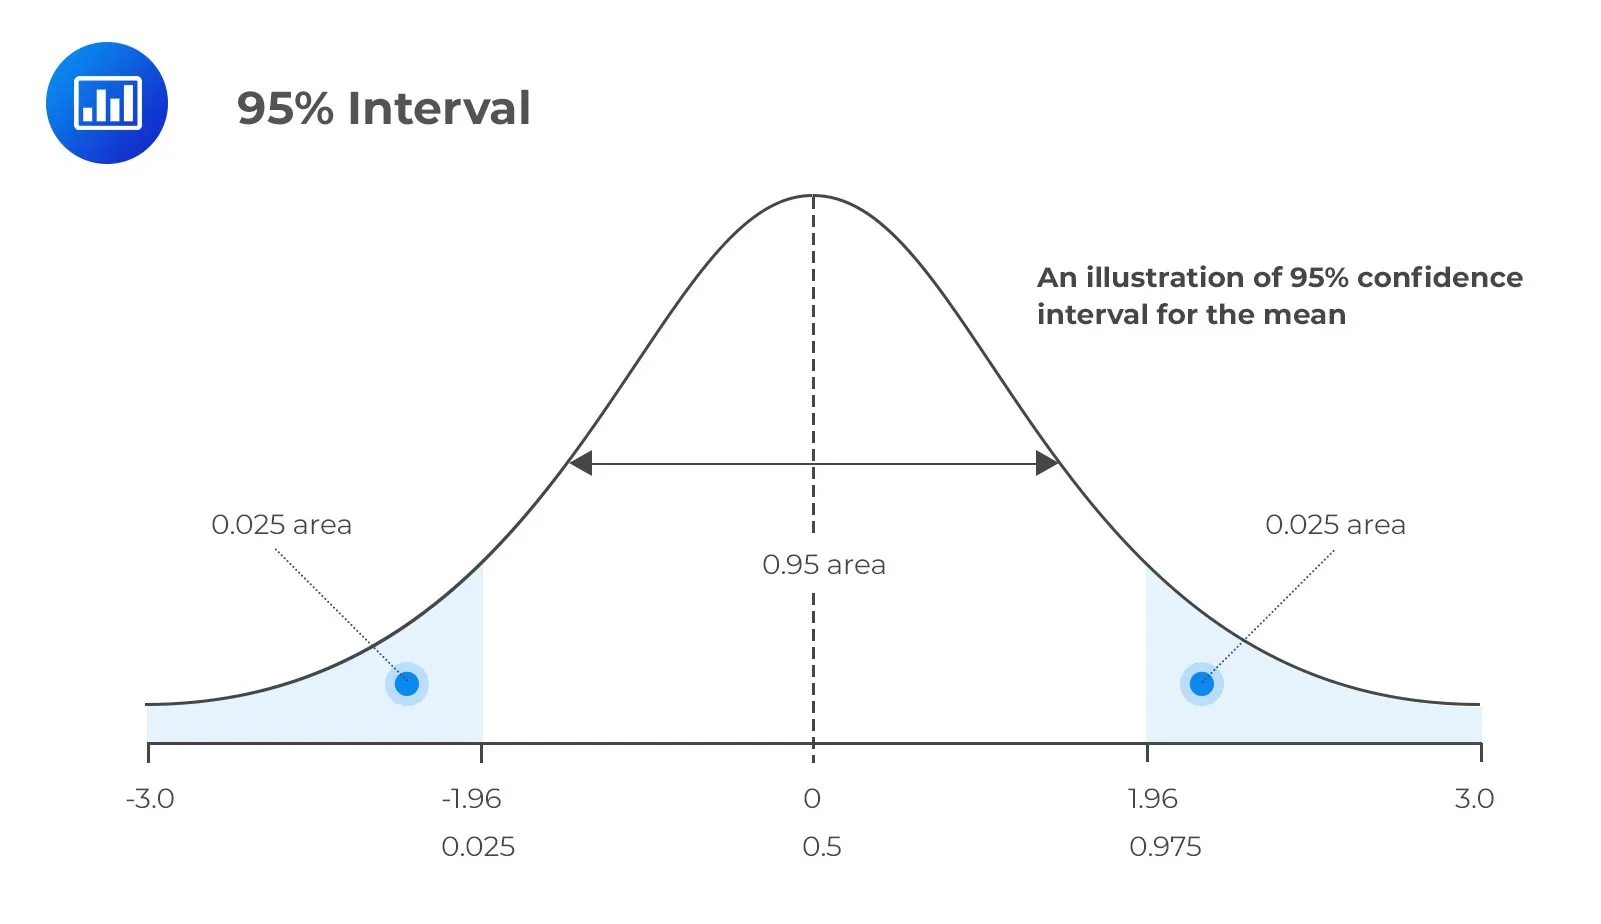
\includegraphics{smoothing/confidence-interval.png}

\marginnote{\begin{footnotesize}

Source:
\href{https://medium.com/@dhaval.sony.504/know-about-confidence-interval-1f66d9ef7d0f}{Dhaval
Raval's Medium article}

\end{footnotesize}}

You can find the Z-score using the following python code:

\begin{Shaded}
\begin{Highlighting}[]
\ImportTok{from}\NormalTok{ scipy.stats }\ImportTok{import}\NormalTok{ norm}

\NormalTok{confidence\_level }\OperatorTok{=} \FloatTok{0.95}
\CommentTok{\# 5\% outside}
\NormalTok{out }\OperatorTok{=} \DecValTok{1} \OperatorTok{{-}}\NormalTok{ confidence\_level}
\CommentTok{\# 0.975 of points to the left of right boundary}
\NormalTok{p }\OperatorTok{=} \DecValTok{1} \OperatorTok{{-}}\NormalTok{ out}\OperatorTok{/}\DecValTok{2}
\CommentTok{\# inverse of cdf: 0.975 of the points will be smaller than what distance (in sigma units)?}
\NormalTok{z\_score }\OperatorTok{=}\NormalTok{ norm.ppf(p)}
\BuiltInTok{print}\NormalTok{(}\SpecialStringTok{f"z{-}score = }\SpecialCharTok{\{}\NormalTok{z\_score}\SpecialCharTok{\}}\SpecialStringTok{"}\NormalTok{)}
\end{Highlighting}
\end{Shaded}

\begin{verbatim}
z-score = 1.959963984540054
\end{verbatim}

If you are still not convinced why we need 0.975 instead of 0.95, read
this \href{https://stackoverflow.com/a/20864883}{excellent response on
stackoverflow}.

SE is the standard error:

\[
SE = \frac{\sigma}{ \sqrt{N} }.
\]

\marginnote{\begin{footnotesize}

\begin{itemize}
\tightlist
\item
  \(\sigma=\) standard deviation.
\item
  \(N=\) number of points.
\end{itemize}

\end{footnotesize}}

We can write a function to calculate the confidence interval of the
mean, and use it with the sliding window:

\begin{Shaded}
\begin{Highlighting}[]
\KeywordTok{def}\NormalTok{ std\_error\_of\_the\_mean(window):}
    \ControlFlowTok{return}\NormalTok{ window.std() }\OperatorTok{/}\NormalTok{ np.sqrt(window.count())}

\KeywordTok{def}\NormalTok{ confidence\_interval(window):}
    \ControlFlowTok{return}\NormalTok{ z\_score }\OperatorTok{*}\NormalTok{ std\_error\_of\_the\_mean(window)}

\NormalTok{df[}\StringTok{\textquotesingle{}std\_error\textquotesingle{}}\NormalTok{] }\OperatorTok{=}\NormalTok{ (}
\NormalTok{                   df[}\StringTok{\textquotesingle{}temp\textquotesingle{}}\NormalTok{].rolling(}\StringTok{\textquotesingle{}3H\textquotesingle{}}\NormalTok{,}
\NormalTok{                                      center}\OperatorTok{=}\VariableTok{True}\NormalTok{)}
\NormalTok{                             .}\BuiltInTok{apply}\NormalTok{(std\_error\_of\_the\_mean)}
\NormalTok{                  )}
\NormalTok{df[}\StringTok{\textquotesingle{}confidence\_int\textquotesingle{}}\NormalTok{] }\OperatorTok{=}\NormalTok{ (}
\NormalTok{                        df[}\StringTok{\textquotesingle{}temp\textquotesingle{}}\NormalTok{].rolling(}\StringTok{\textquotesingle{}3H\textquotesingle{}}\NormalTok{,}
\NormalTok{                                           center}\OperatorTok{=}\VariableTok{True}\NormalTok{)}
\NormalTok{                                  .}\BuiltInTok{apply}\NormalTok{(confidence\_interval)}
\NormalTok{                       )}
\end{Highlighting}
\end{Shaded}

\begin{Shaded}
\begin{Highlighting}[]
\NormalTok{fig, ax }\OperatorTok{=}\NormalTok{ plt.subplots(figsize}\OperatorTok{=}\NormalTok{(}\DecValTok{8}\NormalTok{,}\DecValTok{5}\NormalTok{))}

\NormalTok{plot\_std }\OperatorTok{=}\NormalTok{ ax.fill\_between(df.index,}
\NormalTok{                            df[}\StringTok{\textquotesingle{}mean\textquotesingle{}}\NormalTok{] }\OperatorTok{+}\NormalTok{ df[}\StringTok{\textquotesingle{}confidence\_int\textquotesingle{}}\NormalTok{],}
\NormalTok{                            df[}\StringTok{\textquotesingle{}mean\textquotesingle{}}\NormalTok{] }\OperatorTok{{-}}\NormalTok{ df[}\StringTok{\textquotesingle{}confidence\_int\textquotesingle{}}\NormalTok{],}
\NormalTok{                            color}\OperatorTok{=}\StringTok{"xkcd:pink"}\NormalTok{, alpha}\OperatorTok{=}\FloatTok{0.5}\NormalTok{)}
\NormalTok{plot\_data, }\OperatorTok{=}\NormalTok{ ax.plot(df[}\StringTok{\textquotesingle{}temp\textquotesingle{}}\NormalTok{], color}\OperatorTok{=}\StringTok{\textquotesingle{}black\textquotesingle{}}\NormalTok{, alpha}\OperatorTok{=}\FloatTok{0.3}\NormalTok{)}
\NormalTok{plot\_mean, }\OperatorTok{=}\NormalTok{ax.plot(df[}\StringTok{\textquotesingle{}mean\textquotesingle{}}\NormalTok{], color}\OperatorTok{=}\StringTok{\textquotesingle{}xkcd:hot pink\textquotesingle{}}\NormalTok{)}

\NormalTok{ax.legend([plot\_data, plot\_mean, plot\_std],}
\NormalTok{          [}\StringTok{\textquotesingle{}data\textquotesingle{}}\NormalTok{, }\StringTok{\textquotesingle{}3{-}hour running average\textquotesingle{}}\NormalTok{, }\VerbatimStringTok{r"95}\SpecialCharTok{\% c}\VerbatimStringTok{onfidence interval"}\NormalTok{],}
\NormalTok{          frameon}\OperatorTok{=}\VariableTok{False}\NormalTok{)}

\CommentTok{\# applying the settings to the ax object}
\NormalTok{ax.}\BuiltInTok{set}\NormalTok{(}\OperatorTok{**}\NormalTok{plot\_settings)}
\NormalTok{centered\_dates(ax)}
\CommentTok{\# fig.savefig("YF{-}temperature\_2022\_jan.png", dpi=300)}
\end{Highlighting}
\end{Shaded}

\begin{figure}[H]

{\centering \includegraphics{smoothing/not-only-averages_files/figure-pdf/cell-10-output-1.png}

}

\end{figure}

When the time series has a regular sampling frequency, all positions of
the running window will have the same number of data points in them.
Because the Confidence Interval is proportional to the Standard Error,
and the SE is proportional to the Standard Deviation (\(\sqrt{N}\) is
constant), then the envelope created by the CI is identical to the
envelope created by the standard deviation, up to a multiplying
constant. Nice.

\begin{Shaded}
\begin{Highlighting}[]
\NormalTok{fig, ax }\OperatorTok{=}\NormalTok{ plt.subplots(figsize}\OperatorTok{=}\NormalTok{(}\DecValTok{8}\NormalTok{,}\DecValTok{5}\NormalTok{))}
\NormalTok{plot\_ci, }\OperatorTok{=}\NormalTok{ ax.plot(df[}\StringTok{\textquotesingle{}confidence\_int\textquotesingle{}}\NormalTok{], color}\OperatorTok{=}\StringTok{\textquotesingle{}tab:red\textquotesingle{}}\NormalTok{)}
\NormalTok{plot\_std, }\OperatorTok{=}\NormalTok{ ax.plot(df[}\StringTok{\textquotesingle{}std\textquotesingle{}}\NormalTok{], color}\OperatorTok{=}\StringTok{"black"}\NormalTok{)}
\NormalTok{ax.legend([plot\_ci, plot\_std],}
\NormalTok{          [}\StringTok{\textquotesingle{}confidence interval\textquotesingle{}}\NormalTok{, }\StringTok{\textquotesingle{}standard deviation\textquotesingle{}}\NormalTok{],}
\NormalTok{          frameon}\OperatorTok{=}\VariableTok{False}\NormalTok{)}

\CommentTok{\# applying the settings to the ax object}
\CommentTok{\# ax.set(**plot\_settings)}
\NormalTok{ax.}\BuiltInTok{set}\NormalTok{(xlim}\OperatorTok{=}\NormalTok{[df.index[}\DecValTok{0}\NormalTok{], df.index[}\OperatorTok{{-}}\DecValTok{1}\NormalTok{]])}
\NormalTok{centered\_dates(ax)}
\end{Highlighting}
\end{Shaded}

\begin{figure}[H]

{\centering \includegraphics{smoothing/not-only-averages_files/figure-pdf/cell-11-output-1.png}

}

\end{figure}

\hypertarget{fit}{%
\chapter{fit}\label{fit}}

We will make a little parenthesis to talk about a very important topic:
\textbf{fitting}.

See below temperature data inside and outside a greenhouse, for a period
of about 2 weeks.

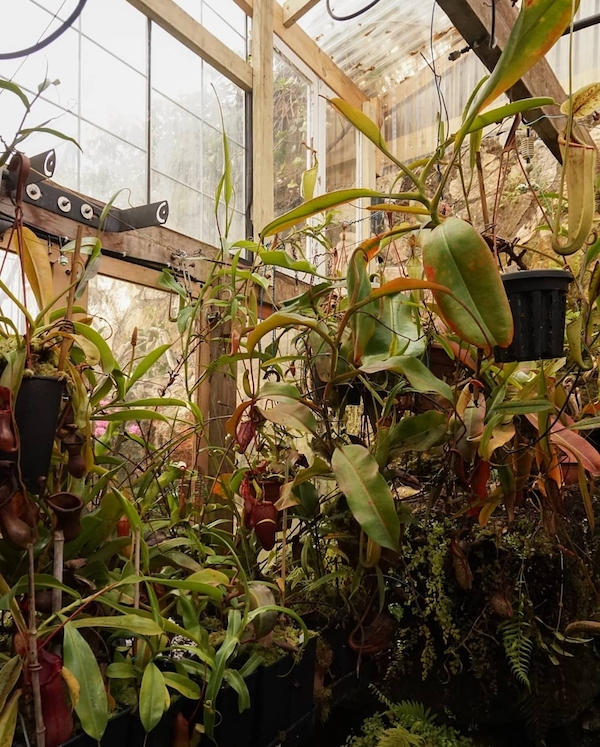
\includegraphics{smoothing/gh_erez.jpg}

\marginnote{\begin{footnotesize}

\href{https://www.google.com/url?sa=t\&rct=j\&q=\&esrc=s\&source=web\&cd=\&cad=rja\&uact=8\&ved=2ahUKEwiQ8bHa0suDAxVMXvEDHVsXCMIQFnoECA0QAQ\&url=https\%3A\%2F\%2Fwww.ynet.co.il\%2Fenvironment-science\%2Farticle\%2Fbkhlgjk49\&usg=AOvVaw25yr2RjpAaEYNQ7DXK03AW\&opi=89978449}{Erez
Feuer's greenhouse}

\end{footnotesize}}

\begin{Shaded}
\begin{Highlighting}[]
\ImportTok{import}\NormalTok{ numpy }\ImportTok{as}\NormalTok{ np}
\ImportTok{import}\NormalTok{ matplotlib.pyplot }\ImportTok{as}\NormalTok{ plt}
\ImportTok{import}\NormalTok{ pandas }\ImportTok{as}\NormalTok{ pd}
\ImportTok{import}\NormalTok{ altair }\ImportTok{as}\NormalTok{ alt}
\ImportTok{from}\NormalTok{ matplotlib.dates }\ImportTok{import}\NormalTok{ DateFormatter}
\ImportTok{import}\NormalTok{ matplotlib.dates }\ImportTok{as}\NormalTok{ mdates}
\ImportTok{import}\NormalTok{ matplotlib.ticker }\ImportTok{as}\NormalTok{ ticker}
\ImportTok{from}\NormalTok{ scipy.optimize }\ImportTok{import}\NormalTok{ curve\_fit}
\ImportTok{import}\NormalTok{ seaborn }\ImportTok{as}\NormalTok{ sns}
\NormalTok{sns.}\BuiltInTok{set}\NormalTok{(style}\OperatorTok{=}\StringTok{"ticks"}\NormalTok{, font\_scale}\OperatorTok{=}\FloatTok{1.5}\NormalTok{)  }\CommentTok{\# white graphs, with large and legible letters}
\CommentTok{\# avoid "SettingWithCopyWarning: A value is trying to be set on a copy of a slice from a DataFrame."}
\NormalTok{pd.options.mode.chained\_assignment }\OperatorTok{=} \VariableTok{None}  \CommentTok{\# default=\textquotesingle{}warn\textquotesingle{}}
\CommentTok{\# \%matplotlib widget}
\end{Highlighting}
\end{Shaded}

\begin{Shaded}
\begin{Highlighting}[]
\NormalTok{df }\OperatorTok{=}\NormalTok{ pd.read\_csv(}\StringTok{\textquotesingle{}greenhouse\_cooling.csv\textquotesingle{}}\NormalTok{, index\_col}\OperatorTok{=}\StringTok{\textquotesingle{}time\textquotesingle{}}\NormalTok{, parse\_dates}\OperatorTok{=}\VariableTok{True}\NormalTok{)}
\CommentTok{\# df}
\end{Highlighting}
\end{Shaded}

\begin{Shaded}
\begin{Highlighting}[]
\NormalTok{fig, ax }\OperatorTok{=}\NormalTok{ plt.subplots(figsize}\OperatorTok{=}\NormalTok{(}\DecValTok{8}\NormalTok{,}\DecValTok{5}\NormalTok{))}

\NormalTok{ax.plot(df[}\StringTok{\textquotesingle{}T\_in\textquotesingle{}}\NormalTok{], c}\OperatorTok{=}\StringTok{\textquotesingle{}tab:blue\textquotesingle{}}\NormalTok{, label}\OperatorTok{=}\StringTok{\textquotesingle{}inside\textquotesingle{}}\NormalTok{)}
\NormalTok{ax.plot(df[}\StringTok{\textquotesingle{}T\_out\textquotesingle{}}\NormalTok{], c}\OperatorTok{=}\StringTok{\textquotesingle{}tab:orange\textquotesingle{}}\NormalTok{, label}\OperatorTok{=}\StringTok{\textquotesingle{}outside\textquotesingle{}}\NormalTok{)}
\NormalTok{ax.}\BuiltInTok{set}\NormalTok{(ylabel}\OperatorTok{=}\StringTok{\textquotesingle{}temperature (°C)\textquotesingle{}}\NormalTok{,}
\NormalTok{       title}\OperatorTok{=}\StringTok{"greenhouse temperatures"}\NormalTok{)}

\CommentTok{\# formating dates on x axis}
\NormalTok{locator }\OperatorTok{=}\NormalTok{ mdates.AutoDateLocator(minticks}\OperatorTok{=}\DecValTok{7}\NormalTok{, maxticks}\OperatorTok{=}\DecValTok{11}\NormalTok{)}
\NormalTok{formatter }\OperatorTok{=}\NormalTok{ mdates.ConciseDateFormatter(locator)}
\NormalTok{ax.xaxis.set\_major\_locator(locator)}
\NormalTok{ax.xaxis.set\_major\_formatter(formatter)}

\NormalTok{ax.legend(frameon}\OperatorTok{=}\VariableTok{False}\NormalTok{)}\OperatorTok{;}
\end{Highlighting}
\end{Shaded}

\begin{figure}[H]

{\centering \includegraphics{smoothing/fit_files/figure-pdf/cell-4-output-1.png}

}

\end{figure}

Every evening, at 20:00, the air conditioning turns on, and we see a
fast decrease in temperature:

\begin{Shaded}
\begin{Highlighting}[]
\NormalTok{df\_fit }\OperatorTok{=}\NormalTok{ df[}\StringTok{\textquotesingle{}2023{-}06{-}29 20:10:00\textquotesingle{}}\NormalTok{:}\StringTok{\textquotesingle{}2023{-}06{-}29 22:00:00\textquotesingle{}}\NormalTok{]}

\NormalTok{fig, ax }\OperatorTok{=}\NormalTok{ plt.subplots(}\DecValTok{2}\NormalTok{, }\DecValTok{1}\NormalTok{, figsize}\OperatorTok{=}\NormalTok{(}\DecValTok{8}\NormalTok{,}\DecValTok{6}\NormalTok{))}
\NormalTok{fig.subplots\_adjust(hspace}\OperatorTok{=}\FloatTok{0.4}\NormalTok{)  }\CommentTok{\# Adjust the vertical space between subplots}

\NormalTok{ax[}\DecValTok{0}\NormalTok{].plot(df.loc[}\StringTok{\textquotesingle{}2023{-}06{-}29 16:10:00\textquotesingle{}}\NormalTok{:}\StringTok{\textquotesingle{}2023{-}06{-}30 16:00:00\textquotesingle{}}\NormalTok{, }\StringTok{\textquotesingle{}T\_in\textquotesingle{}}\NormalTok{], color}\OperatorTok{=}\StringTok{\textquotesingle{}tab:green\textquotesingle{}}\NormalTok{)}
\NormalTok{ax[}\DecValTok{0}\NormalTok{].}\BuiltInTok{set}\NormalTok{(ylabel}\OperatorTok{=}\StringTok{\textquotesingle{}temperature (°C)\textquotesingle{}}\NormalTok{,}
\NormalTok{       title}\OperatorTok{=}\StringTok{"temperature inside the greenhouse"}\NormalTok{)}

\NormalTok{ax[}\DecValTok{1}\NormalTok{].scatter(df\_fit[}\StringTok{\textquotesingle{}T\_in\textquotesingle{}}\NormalTok{].index, df\_fit[}\StringTok{\textquotesingle{}T\_in\textquotesingle{}}\NormalTok{], color}\OperatorTok{=}\StringTok{\textquotesingle{}tab:green\textquotesingle{}}\NormalTok{)}
\NormalTok{ax[}\DecValTok{1}\NormalTok{].}\BuiltInTok{set}\NormalTok{(ylabel}\OperatorTok{=}\StringTok{\textquotesingle{}temperature (°C)\textquotesingle{}}\NormalTok{,)}

\CommentTok{\# formating dates on x axis}
\NormalTok{locator }\OperatorTok{=}\NormalTok{ mdates.AutoDateLocator(minticks}\OperatorTok{=}\DecValTok{7}\NormalTok{, maxticks}\OperatorTok{=}\DecValTok{11}\NormalTok{)}
\NormalTok{formatter }\OperatorTok{=}\NormalTok{ mdates.ConciseDateFormatter(locator)}
\NormalTok{ax[}\DecValTok{0}\NormalTok{].xaxis.set\_major\_locator(locator)}
\NormalTok{ax[}\DecValTok{0}\NormalTok{].xaxis.set\_major\_formatter(formatter)}

\NormalTok{locator }\OperatorTok{=}\NormalTok{ mdates.AutoDateLocator(minticks}\OperatorTok{=}\DecValTok{7}\NormalTok{, maxticks}\OperatorTok{=}\DecValTok{11}\NormalTok{)}
\NormalTok{formatter }\OperatorTok{=}\NormalTok{ mdates.ConciseDateFormatter(locator)}
\NormalTok{ax[}\DecValTok{1}\NormalTok{].xaxis.set\_major\_locator(locator)}
\NormalTok{ax[}\DecValTok{1}\NormalTok{].xaxis.set\_major\_formatter(formatter)}
\end{Highlighting}
\end{Shaded}

\begin{figure}[H]

{\centering \includegraphics{smoothing/fit_files/figure-pdf/cell-5-output-1.png}

}

\end{figure}

The AC is able to bring the temperature down, but up to a limit. The AC
can work at a maximum given power, and the cooler it is outside, the
more effectively the AC will be able to bring down the temperature
inside the greenhouse. We can imagine that the AC behaves as an
effective external environment to the greenhouse, and the greenhouse
cools down according to
\href{https://en.wikipedia.org/wiki/Newton\%27s_law_of_cooling}{Newton's
law of cooling}:

\[
\frac{dT}{dt} = r\cdot (T_{\text{env}}-T)
\]

\marginnote{\begin{footnotesize}

\begin{itemize}
\tightlist
\item
  \(T=\) the greenhouse temperature
\item
  \(T_{\text{env}}=\) the outside environment temperature
\item
  \(r=\) coefficient of heat transfer.
\end{itemize}

\end{footnotesize}}

The cooling rate is proportional to the difference in temperature
between the inside and outside. Assuming \(T_{\text{env}}\) and \(r\) to
be constant, the solution of this differential equation is:

\[
T(t) = T_{\text{env}} + \left(T_0 - T_{\text{env}} \right)e^{-rt}.
\]

\marginnote{\begin{footnotesize}

\begin{itemize}
\tightlist
\item
  \(T_0=\) the initial greenhouse temperature
\end{itemize}

\end{footnotesize}}

We want to check if the temperature measured inside the greenhouse
behaves like Newton's law of cooling, and if so, what can we say about
the cooling coefficient \(r\) and about \(T_{\text{env}}\).

\hypertarget{linear-fit}{%
\section{linear fit}\label{linear-fit}}

The following is a \textbf{very short} introduction to curve fitting.
The natural place to start is with a linear fit.

\begin{Shaded}
\begin{Highlighting}[]
\CommentTok{\# the "fit" process can\textquotesingle{}t deal with datetimes}
\CommentTok{\# we therefore make a new column \textquotesingle{}minutes\textquotesingle{}, that will be used here}
\NormalTok{df\_fit[}\StringTok{\textquotesingle{}minutes\textquotesingle{}}\NormalTok{] }\OperatorTok{=}\NormalTok{ (df\_fit.index }\OperatorTok{{-}}\NormalTok{ df\_fit.index[}\DecValTok{0}\NormalTok{]).total\_seconds() }\OperatorTok{/} \DecValTok{60}
\CommentTok{\# linear Fit (degree 1)}
\NormalTok{degree }\OperatorTok{=} \DecValTok{1}
\NormalTok{coeffs }\OperatorTok{=}\NormalTok{ np.polyfit(df\_fit[}\StringTok{\textquotesingle{}minutes\textquotesingle{}}\NormalTok{], df\_fit[}\StringTok{\textquotesingle{}T\_in\textquotesingle{}}\NormalTok{], degree)}
\CommentTok{\# linear Function}
\NormalTok{linear\_function }\OperatorTok{=}\NormalTok{ np.poly1d(coeffs)}
\end{Highlighting}
\end{Shaded}

\begin{Shaded}
\begin{Highlighting}[]
\NormalTok{fig, ax }\OperatorTok{=}\NormalTok{ plt.subplots(figsize}\OperatorTok{=}\NormalTok{(}\DecValTok{8}\NormalTok{,}\DecValTok{5}\NormalTok{))}

\NormalTok{ax.scatter(df\_fit[}\StringTok{\textquotesingle{}minutes\textquotesingle{}}\NormalTok{], df\_fit[}\StringTok{\textquotesingle{}T\_in\textquotesingle{}}\NormalTok{],}
\NormalTok{           color}\OperatorTok{=}\StringTok{\textquotesingle{}tab:green\textquotesingle{}}\NormalTok{, label}\OperatorTok{=}\StringTok{\textquotesingle{}data\textquotesingle{}}\NormalTok{)}
\NormalTok{ax.plot(df\_fit[}\StringTok{\textquotesingle{}minutes\textquotesingle{}}\NormalTok{], linear\_function(df\_fit[}\StringTok{\textquotesingle{}minutes\textquotesingle{}}\NormalTok{]),}
\NormalTok{        color}\OperatorTok{=}\StringTok{\textquotesingle{}black\textquotesingle{}}\NormalTok{, label}\OperatorTok{=}\StringTok{\textquotesingle{}linear fit\textquotesingle{}}\NormalTok{)}

\NormalTok{ax.}\BuiltInTok{set}\NormalTok{(xlabel}\OperatorTok{=}\StringTok{\textquotesingle{}minutes\textquotesingle{}}\NormalTok{,}
\NormalTok{       ylabel}\OperatorTok{=}\StringTok{\textquotesingle{}temperature (°C)\textquotesingle{}}\NormalTok{,}
\NormalTok{       title}\OperatorTok{=}\StringTok{"temperature inside the greenhouse"}\NormalTok{)}

\NormalTok{ax.legend(frameon}\OperatorTok{=}\VariableTok{False}\NormalTok{)}
\BuiltInTok{print}\NormalTok{(}\SpecialStringTok{f"starting at }\SpecialCharTok{\{}\NormalTok{coeffs[}\DecValTok{1}\NormalTok{]}\SpecialCharTok{:.2f\}}\SpecialStringTok{ degrees,}\CharTok{\textbackslash{}n}\SpecialStringTok{the temperature decreases by }\SpecialCharTok{\{}\OperatorTok{{-}}\NormalTok{coeffs[}\DecValTok{0}\NormalTok{]}\SpecialCharTok{:.2f\}}\SpecialStringTok{ degrees every minute."}\NormalTok{)}
\end{Highlighting}
\end{Shaded}

\begin{verbatim}
starting at 19.80 degrees,
the temperature decreases by 0.05 degrees every minute.
\end{verbatim}

\begin{figure}[H]

{\centering \includegraphics{smoothing/fit_files/figure-pdf/cell-7-output-2.png}

}

\end{figure}

The line above is the ``best'' straight line that describes our data.
Defining the residual as the difference between our data and our model
(straight line),

\[
e = T_{\text{data}} - T_{\text{model}},
\]

the straight line above is the one that \textbf{minimizes} the sum of
the squares of residuals. For this reason, the method used above to fit
a curve to the data is called ``least-squares method''.

\marginnote{\begin{footnotesize}

it minimizes the sum

\[
S = \sum_i e_i^2
\]

\end{footnotesize}}

Can we do better than a straight line?

\hypertarget{polynomial-fit}{%
\section{polynomial fit}\label{polynomial-fit}}

\begin{Shaded}
\begin{Highlighting}[]
\CommentTok{\# polynomial fit (degree 2)}
\NormalTok{degree }\OperatorTok{=} \DecValTok{2}
\NormalTok{coeffs2 }\OperatorTok{=}\NormalTok{ np.polyfit(df\_fit[}\StringTok{\textquotesingle{}minutes\textquotesingle{}}\NormalTok{], df\_fit[}\StringTok{\textquotesingle{}T\_in\textquotesingle{}}\NormalTok{], degree)}
\NormalTok{quad\_function }\OperatorTok{=}\NormalTok{ np.poly1d(coeffs2)}

\CommentTok{\# polynomial fit (degree 2)}
\NormalTok{degree }\OperatorTok{=} \DecValTok{3}
\NormalTok{coeffs3 }\OperatorTok{=}\NormalTok{ np.polyfit(df\_fit[}\StringTok{\textquotesingle{}minutes\textquotesingle{}}\NormalTok{], df\_fit[}\StringTok{\textquotesingle{}T\_in\textquotesingle{}}\NormalTok{], degree)}
\NormalTok{cubic\_function }\OperatorTok{=}\NormalTok{ np.poly1d(coeffs3)}
\end{Highlighting}
\end{Shaded}

\begin{Shaded}
\begin{Highlighting}[]
\NormalTok{fig, ax }\OperatorTok{=}\NormalTok{ plt.subplots(figsize}\OperatorTok{=}\NormalTok{(}\DecValTok{8}\NormalTok{,}\DecValTok{5}\NormalTok{))}

\NormalTok{ax.scatter(df\_fit[}\StringTok{\textquotesingle{}minutes\textquotesingle{}}\NormalTok{], df\_fit[}\StringTok{\textquotesingle{}T\_in\textquotesingle{}}\NormalTok{],}
\NormalTok{           color}\OperatorTok{=}\StringTok{\textquotesingle{}tab:green\textquotesingle{}}\NormalTok{, label}\OperatorTok{=}\StringTok{\textquotesingle{}data\textquotesingle{}}\NormalTok{)}
\NormalTok{ax.plot(df\_fit[}\StringTok{\textquotesingle{}minutes\textquotesingle{}}\NormalTok{], quad\_function(df\_fit[}\StringTok{\textquotesingle{}minutes\textquotesingle{}}\NormalTok{]),}
\NormalTok{        color}\OperatorTok{=}\StringTok{\textquotesingle{}black\textquotesingle{}}\NormalTok{, label}\OperatorTok{=}\StringTok{\textquotesingle{}order = 2\textquotesingle{}}\NormalTok{)}
\NormalTok{ax.plot(df\_fit[}\StringTok{\textquotesingle{}minutes\textquotesingle{}}\NormalTok{], cubic\_function(df\_fit[}\StringTok{\textquotesingle{}minutes\textquotesingle{}}\NormalTok{]),}
\NormalTok{        color}\OperatorTok{=}\StringTok{\textquotesingle{}tab:olive\textquotesingle{}}\NormalTok{, label}\OperatorTok{=}\StringTok{\textquotesingle{}order = 3\textquotesingle{}}\NormalTok{)}

\NormalTok{ax.}\BuiltInTok{set}\NormalTok{(xlabel}\OperatorTok{=}\StringTok{\textquotesingle{}minutes\textquotesingle{}}\NormalTok{,}
\NormalTok{       ylabel}\OperatorTok{=}\StringTok{\textquotesingle{}temperature (°C)\textquotesingle{}}\NormalTok{,}
\NormalTok{       title}\OperatorTok{=}\StringTok{"temperature inside the greenhouse"}\NormalTok{)}
\NormalTok{ax.legend(frameon}\OperatorTok{=}\VariableTok{False}\NormalTok{)}
\end{Highlighting}
\end{Shaded}

\begin{verbatim}
<matplotlib.legend.Legend at 0x7fd0a0833eb0>
\end{verbatim}

\begin{figure}[H]

{\centering 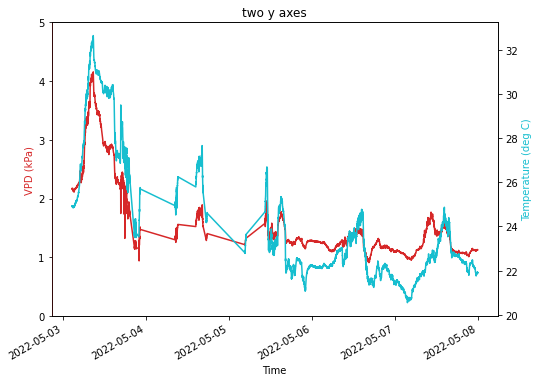
\includegraphics{smoothing/fit_files/figure-pdf/cell-9-output-2.png}

}

\end{figure}

\hypertarget{any-function-you-want}{%
\section{any function you want}\label{any-function-you-want}}

Now let's get back to our original assumption, that the greenhouse cools
according to Newton's cooling law. We can still use the least-squares
method for any function we want!

\begin{Shaded}
\begin{Highlighting}[]
\KeywordTok{def}\NormalTok{ cooling(t, T\_env, T0, r):}
    \CommentTok{"""}
\CommentTok{    t = time}
\CommentTok{    other stuff = parameters to be fitted}
\CommentTok{    """}
    \ControlFlowTok{return}\NormalTok{ T\_env }\OperatorTok{+}\NormalTok{ (T0 }\OperatorTok{{-}}\NormalTok{ T\_env)}\OperatorTok{*}\NormalTok{np.exp(}\OperatorTok{{-}}\NormalTok{r}\OperatorTok{*}\NormalTok{t)}
\end{Highlighting}
\end{Shaded}

\begin{Shaded}
\begin{Highlighting}[]
\NormalTok{t }\OperatorTok{=}\NormalTok{ df\_fit[}\StringTok{\textquotesingle{}minutes\textquotesingle{}}\NormalTok{].values}
\NormalTok{y }\OperatorTok{=}\NormalTok{ df\_fit[}\StringTok{\textquotesingle{}T\_in\textquotesingle{}}\NormalTok{].values}

\NormalTok{T\_init }\OperatorTok{=}\NormalTok{ df\_fit[}\StringTok{\textquotesingle{}T\_in\textquotesingle{}}\NormalTok{][}\DecValTok{0}\NormalTok{]}

\NormalTok{popt, pcov }\OperatorTok{=}\NormalTok{ curve\_fit(f}\OperatorTok{=}\NormalTok{cooling,             }\CommentTok{\# model function}
\NormalTok{                     xdata}\OperatorTok{=}\NormalTok{t,                 }\CommentTok{\# x data}
\NormalTok{                     ydata}\OperatorTok{=}\NormalTok{y,                 }\CommentTok{\# y data}
\NormalTok{                     p0}\OperatorTok{=}\NormalTok{(}\DecValTok{2}\NormalTok{, T\_init, }\FloatTok{0.5}\NormalTok{),     }\CommentTok{\# initial guess of the parameters}
\NormalTok{                     )}
\BuiltInTok{print}\NormalTok{(}\SpecialStringTok{f"the optimal parameters are }\SpecialCharTok{\{}\NormalTok{popt}\SpecialCharTok{\}}\SpecialStringTok{"}\NormalTok{)}
\end{Highlighting}
\end{Shaded}

\begin{verbatim}
the optimal parameters are [14.01663586 21.0074623   0.02121802]
\end{verbatim}

\begin{Shaded}
\begin{Highlighting}[]
\NormalTok{fig, ax }\OperatorTok{=}\NormalTok{ plt.subplots(sharex}\OperatorTok{=}\VariableTok{True}\NormalTok{)}

\NormalTok{ax.scatter(df\_fit[}\StringTok{\textquotesingle{}minutes\textquotesingle{}}\NormalTok{], df\_fit[}\StringTok{\textquotesingle{}T\_in\textquotesingle{}}\NormalTok{],}
\NormalTok{           color}\OperatorTok{=}\StringTok{\textquotesingle{}tab:green\textquotesingle{}}\NormalTok{, label}\OperatorTok{=}\StringTok{\textquotesingle{}data\textquotesingle{}}\NormalTok{)}
\NormalTok{ax.plot(t, cooling(t, }\OperatorTok{*}\NormalTok{popt),}
\NormalTok{        color}\OperatorTok{=}\StringTok{\textquotesingle{}black\textquotesingle{}}\NormalTok{, label}\OperatorTok{=}\StringTok{\textquotesingle{}exponential fit\textquotesingle{}}\NormalTok{)}

\NormalTok{ax.}\BuiltInTok{set}\NormalTok{(xlabel}\OperatorTok{=}\StringTok{\textquotesingle{}minutes\textquotesingle{}}\NormalTok{,}
\NormalTok{       ylabel}\OperatorTok{=}\StringTok{\textquotesingle{}temperature (°C)\textquotesingle{}}\NormalTok{,}
\NormalTok{       title}\OperatorTok{=}\StringTok{"temperature inside the greenhouse"}\NormalTok{)}

\NormalTok{ax.legend(frameon}\OperatorTok{=}\VariableTok{False}\NormalTok{)}
\end{Highlighting}
\end{Shaded}

\begin{verbatim}
<matplotlib.legend.Legend at 0x7fd0b0140850>
\end{verbatim}

\begin{figure}[H]

{\centering 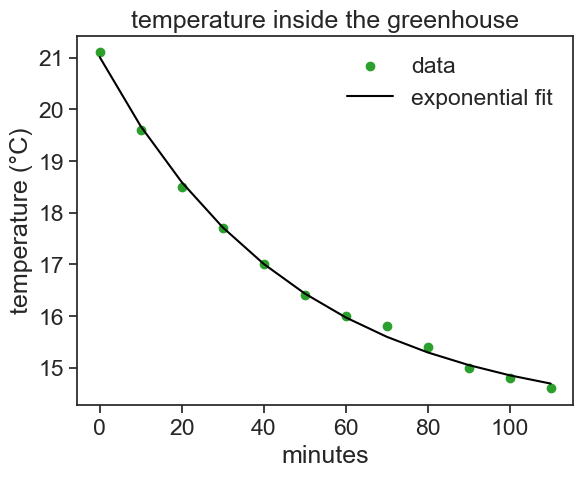
\includegraphics{smoothing/fit_files/figure-pdf/cell-12-output-2.png}

}

\end{figure}

That looks really good :)

We can use curve fitting to retrieve important parameters from our data.
Let's write a function that executes the fit and returns two of the
fitted parameters: \texttt{T\_env} and \texttt{r}.

\begin{Shaded}
\begin{Highlighting}[]
\KeywordTok{def}\NormalTok{ run\_fit(data):}
\NormalTok{    data[}\StringTok{\textquotesingle{}minutes\textquotesingle{}}\NormalTok{] }\OperatorTok{=}\NormalTok{ (data.index }\OperatorTok{{-}}\NormalTok{ data.index[}\DecValTok{0}\NormalTok{]).total\_seconds() }\OperatorTok{/} \DecValTok{60}
\NormalTok{    t }\OperatorTok{=}\NormalTok{ data[}\StringTok{\textquotesingle{}minutes\textquotesingle{}}\NormalTok{].values}
\NormalTok{    y }\OperatorTok{=}\NormalTok{ data[}\StringTok{\textquotesingle{}T\_in\textquotesingle{}}\NormalTok{].values}
\NormalTok{    T\_init }\OperatorTok{=}\NormalTok{ data[}\StringTok{\textquotesingle{}T\_in\textquotesingle{}}\NormalTok{][}\DecValTok{0}\NormalTok{]}
\NormalTok{    popt, pcov }\OperatorTok{=}\NormalTok{ curve\_fit(f}\OperatorTok{=}\NormalTok{cooling,             }\CommentTok{\# model function}
\NormalTok{                        xdata}\OperatorTok{=}\NormalTok{t,              }\CommentTok{\# x data}
\NormalTok{                        ydata}\OperatorTok{=}\NormalTok{y,              }\CommentTok{\# y data}
\NormalTok{                        p0}\OperatorTok{=}\NormalTok{(}\DecValTok{2}\NormalTok{, T\_init, }\FloatTok{0.5}\NormalTok{),   }\CommentTok{\# initial guess of the parameters}
\NormalTok{                        )}
    \ControlFlowTok{return}\NormalTok{ popt[}\DecValTok{0}\NormalTok{],popt[}\DecValTok{2}\NormalTok{]}
\end{Highlighting}
\end{Shaded}

We now apply this function to several consecutive evenings, and we keep
the results in a new dataframe.

\begin{Shaded}
\begin{Highlighting}[]
\NormalTok{df\_night }\OperatorTok{=}\NormalTok{ df.between\_time(}\StringTok{\textquotesingle{}20:01\textquotesingle{}}\NormalTok{, }\StringTok{\textquotesingle{}22:01\textquotesingle{}}\NormalTok{, inclusive}\OperatorTok{=}\StringTok{\textquotesingle{}left\textquotesingle{}}\NormalTok{)}

\CommentTok{\# group by day and apply the function}
\CommentTok{\# this is where the magic happens.}
\CommentTok{\# if you are not familiar with "groupby", this will be hard to understand}
\NormalTok{result\_series }\OperatorTok{=}\NormalTok{ df\_night.groupby(df\_night.index.date).}\BuiltInTok{apply}\NormalTok{(run\_fit)}

\CommentTok{\# convert the series to a dataframe}
\NormalTok{result\_df }\OperatorTok{=}\NormalTok{ pd.DataFrame(result\_series.tolist(), index}\OperatorTok{=}\NormalTok{result\_series.index, columns}\OperatorTok{=}\NormalTok{[}\StringTok{\textquotesingle{}T\_env\textquotesingle{}}\NormalTok{, }\StringTok{\textquotesingle{}r\textquotesingle{}}\NormalTok{])}
\NormalTok{result\_df.index }\OperatorTok{=}\NormalTok{ pd.to\_datetime(result\_df.index)}
\NormalTok{result\_df}
\end{Highlighting}
\end{Shaded}

\begin{longtable}[]{@{}lll@{}}
\toprule\noalign{}
& T\_env & r \\
\midrule\noalign{}
\endhead
\bottomrule\noalign{}
\endlastfoot
2023-06-25 & 13.275540 & 0.019354 \\
2023-06-26 & 13.331949 & 0.027034 \\
2023-06-27 & 13.254827 & 0.018753 \\
2023-06-28 & 13.392919 & 0.020449 \\
2023-06-29 & 14.016636 & 0.021218 \\
2023-06-30 & 13.807517 & 0.021749 \\
2023-07-01 & 14.994207 & 0.023504 \\
2023-07-02 & 14.314220 & 0.023705 \\
2023-07-03 & 14.585848 & 0.019438 \\
2023-07-04 & 14.377220 & 0.019504 \\
2023-07-05 & 14.814939 & 0.021202 \\
2023-07-06 & 14.667792 & 0.022264 \\
2023-07-07 & 15.535115 & 0.024421 \\
\end{longtable}

\begin{Shaded}
\begin{Highlighting}[]
\NormalTok{fig, ax }\OperatorTok{=}\NormalTok{ plt.subplots(}\DecValTok{3}\NormalTok{,}\DecValTok{1}\NormalTok{,sharex}\OperatorTok{=}\VariableTok{True}\NormalTok{, figsize}\OperatorTok{=}\NormalTok{(}\DecValTok{8}\NormalTok{,}\DecValTok{8}\NormalTok{))}

\NormalTok{ax[}\DecValTok{0}\NormalTok{].plot(df[}\StringTok{\textquotesingle{}T\_in\textquotesingle{}}\NormalTok{], c}\OperatorTok{=}\StringTok{\textquotesingle{}tab:blue\textquotesingle{}}\NormalTok{, label}\OperatorTok{=}\StringTok{\textquotesingle{}inside\textquotesingle{}}\NormalTok{)}
\NormalTok{ax[}\DecValTok{0}\NormalTok{].plot(df[}\StringTok{\textquotesingle{}T\_out\textquotesingle{}}\NormalTok{], c}\OperatorTok{=}\StringTok{\textquotesingle{}tab:orange\textquotesingle{}}\NormalTok{, label}\OperatorTok{=}\StringTok{\textquotesingle{}outside\textquotesingle{}}\NormalTok{)}
\NormalTok{ax[}\DecValTok{0}\NormalTok{].}\BuiltInTok{set}\NormalTok{(ylabel}\OperatorTok{=}\StringTok{\textquotesingle{}temperature (°C)\textquotesingle{}}\NormalTok{,}
\NormalTok{          title}\OperatorTok{=}\StringTok{"actual temperatures"}\NormalTok{,}
\NormalTok{          ylim}\OperatorTok{=}\NormalTok{[}\DecValTok{10}\NormalTok{,}\DecValTok{45}\NormalTok{])}

\CommentTok{\# formating dates on x axis}
\NormalTok{locator }\OperatorTok{=}\NormalTok{ mdates.AutoDateLocator(minticks}\OperatorTok{=}\DecValTok{7}\NormalTok{, maxticks}\OperatorTok{=}\DecValTok{11}\NormalTok{)}
\NormalTok{formatter }\OperatorTok{=}\NormalTok{ mdates.ConciseDateFormatter(locator)}
\NormalTok{ax[}\DecValTok{0}\NormalTok{].xaxis.set\_major\_locator(locator)}
\NormalTok{ax[}\DecValTok{0}\NormalTok{].xaxis.set\_major\_formatter(formatter)}

\NormalTok{ax[}\DecValTok{0}\NormalTok{].legend(ncol}\OperatorTok{=}\DecValTok{2}\NormalTok{, loc}\OperatorTok{=}\StringTok{\textquotesingle{}upper center\textquotesingle{}}\NormalTok{, frameon}\OperatorTok{=}\VariableTok{False}\NormalTok{)}

\NormalTok{ax[}\DecValTok{1}\NormalTok{].plot(result\_df[}\StringTok{\textquotesingle{}r\textquotesingle{}}\NormalTok{], color}\OperatorTok{=}\StringTok{\textquotesingle{}black\textquotesingle{}}\NormalTok{)}
\NormalTok{ax[}\DecValTok{1}\NormalTok{].}\BuiltInTok{set}\NormalTok{(ylabel}\OperatorTok{=}\VerbatimStringTok{r"parameter $r$"}\NormalTok{,}
\NormalTok{          ylim}\OperatorTok{=}\NormalTok{[}\DecValTok{0}\NormalTok{, }\FloatTok{0.04}\NormalTok{])}

\NormalTok{ax[}\DecValTok{2}\NormalTok{].plot(result\_df[}\StringTok{\textquotesingle{}T\_env\textquotesingle{}}\NormalTok{], color}\OperatorTok{=}\StringTok{\textquotesingle{}black\textquotesingle{}}\NormalTok{)}
\NormalTok{ax2b }\OperatorTok{=}\NormalTok{ ax[}\DecValTok{2}\NormalTok{].twinx()}
\NormalTok{ax2b.plot(df\_night[}\StringTok{\textquotesingle{}T\_out\textquotesingle{}}\NormalTok{].resample(}\StringTok{\textquotesingle{}D\textquotesingle{}}\NormalTok{).mean(), color}\OperatorTok{=}\StringTok{\textquotesingle{}tab:orange\textquotesingle{}}\NormalTok{)}
\NormalTok{ax[}\DecValTok{2}\NormalTok{].}\BuiltInTok{set}\NormalTok{(ylim}\OperatorTok{=}\NormalTok{[}\DecValTok{12}\NormalTok{, }\DecValTok{17}\NormalTok{])}
\NormalTok{ax2b.}\BuiltInTok{set}\NormalTok{(ylim}\OperatorTok{=}\NormalTok{[}\DecValTok{19}\NormalTok{, }\DecValTok{24}\NormalTok{],}
\NormalTok{        ylabel}\OperatorTok{=}\StringTok{\textquotesingle{}outside temperature\textquotesingle{}}\NormalTok{)}
\CommentTok{\# color the xticks}
\ControlFlowTok{for}\NormalTok{ tick }\KeywordTok{in}\NormalTok{ ax[}\DecValTok{2}\NormalTok{].get\_yticklabels():}
\NormalTok{    tick.set\_color(}\StringTok{\textquotesingle{}tab:orange\textquotesingle{}}\NormalTok{)}
\CommentTok{\# color the xlabel}
\NormalTok{ax[}\DecValTok{2}\NormalTok{].set\_ylabel(}\VerbatimStringTok{r\textquotesingle{}"outside" temp.\textquotesingle{}}\OperatorTok{+}\StringTok{\textquotesingle{}}\CharTok{\textbackslash{}n}\StringTok{inferred from}\CharTok{\textbackslash{}n}\StringTok{analysis\textquotesingle{}}\NormalTok{, color}\OperatorTok{=}\StringTok{\textquotesingle{}tab:orange\textquotesingle{}}\NormalTok{)}
\end{Highlighting}
\end{Shaded}

\begin{verbatim}
Text(0, 0.5, '"outside" temp.\ninferred from\nanalysis')
\end{verbatim}

\begin{figure}[H]

{\centering 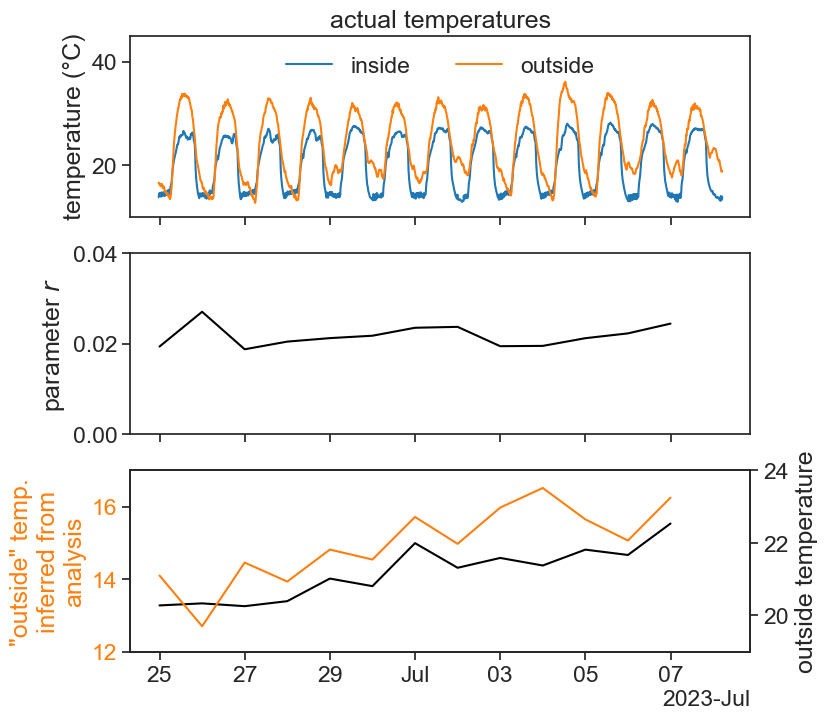
\includegraphics{smoothing/fit_files/figure-pdf/cell-15-output-2.png}

}

\end{figure}

Conclusions:

\begin{enumerate}
\def\labelenumi{\arabic{enumi}.}
\tightlist
\item
  The cooling coefficient \(r\) seems quite stable throughout the two
  weeks of measurements. This probably says that the greenhouse and AC
  properties did not change much. For instance, the greenhouse thermal
  insulation stayed constant, and the AC power output stayed constant.
\item
  The AC tracks very well the outside temperature! This is to say: the
  AC works better (more easily) when temperatures outsides are low, and
  vice-versa.
\end{enumerate}

\hypertarget{savitzkygolay}{%
\chapter{Savitzky--Golay}\label{savitzkygolay}}

The Savitzky-Golay filter, also known as
\href{https://en.wikipedia.org/wiki/Local_regression}{LOESS}, smoothes a
noisy signal by performing a polynomial fit over a sliding window.

Polynomial fit of order 3, window size = 51 pts

Polynomial fit of order 2, window size = 51 pts

The simulations look different because the order of the polynomial makes
a very different impression on us, but in reality the outcome of the two
filtering is almost identical:

\begin{Shaded}
\begin{Highlighting}[]
\ImportTok{import}\NormalTok{ numpy }\ImportTok{as}\NormalTok{ np}
\ImportTok{import}\NormalTok{ matplotlib.pyplot }\ImportTok{as}\NormalTok{ plt}
\ImportTok{import}\NormalTok{ pandas }\ImportTok{as}\NormalTok{ pd}
\ImportTok{from}\NormalTok{ matplotlib.dates }\ImportTok{import}\NormalTok{ DateFormatter}
\ImportTok{import}\NormalTok{ matplotlib.dates }\ImportTok{as}\NormalTok{ mdates}
\ImportTok{import}\NormalTok{ datetime }\ImportTok{as}\NormalTok{ dt}
\ImportTok{import}\NormalTok{ matplotlib.ticker }\ImportTok{as}\NormalTok{ ticker}
\ImportTok{from}\NormalTok{ scipy.signal }\ImportTok{import}\NormalTok{ savgol\_filter}
\ImportTok{import}\NormalTok{ os}
\ImportTok{import}\NormalTok{ warnings}
\ImportTok{import}\NormalTok{ scipy}
\CommentTok{\# Suppress FutureWarnings}
\NormalTok{warnings.simplefilter(action}\OperatorTok{=}\StringTok{\textquotesingle{}ignore\textquotesingle{}}\NormalTok{, category}\OperatorTok{=}\PreprocessorTok{FutureWarning}\NormalTok{)}
\ImportTok{import}\NormalTok{ seaborn }\ImportTok{as}\NormalTok{ sns}
\NormalTok{sns.}\BuiltInTok{set}\NormalTok{(style}\OperatorTok{=}\StringTok{"ticks"}\NormalTok{, font\_scale}\OperatorTok{=}\FloatTok{1.5}\NormalTok{)  }\CommentTok{\# white graphs, with large and legible letters}
\CommentTok{\# \%matplotlib widget}
\end{Highlighting}
\end{Shaded}

\begin{Shaded}
\begin{Highlighting}[]
\CommentTok{\# dirty trick to have dates in the middle of the 24{-}hour period}
\CommentTok{\# make minor ticks in the middle, put the labels there!}
\CommentTok{\# from https://matplotlib.org/stable/gallery/ticks/centered\_ticklabels.html}

\KeywordTok{def}\NormalTok{ centered\_dates(ax):}
\NormalTok{    date\_form }\OperatorTok{=}\NormalTok{ DateFormatter(}\StringTok{"}\SpecialCharTok{\%d}\StringTok{ \%b"}\NormalTok{)  }\CommentTok{\# \%d 3{-}letter{-}Month}
    \CommentTok{\# major ticks at midnight, every day}
\NormalTok{    ax.xaxis.set\_major\_locator(mdates.DayLocator(interval}\OperatorTok{=}\DecValTok{1}\NormalTok{))}
\NormalTok{    ax.xaxis.set\_major\_formatter(date\_form)}
    \CommentTok{\# minor ticks at noon, every day}
\NormalTok{    ax.xaxis.set\_minor\_locator(mdates.HourLocator(byhour}\OperatorTok{=}\NormalTok{[}\DecValTok{12}\NormalTok{]))}
    \CommentTok{\# erase major tick labels}
\NormalTok{    ax.xaxis.set\_major\_formatter(ticker.NullFormatter())}
    \CommentTok{\# set minor tick labels as define above}
\NormalTok{    ax.xaxis.set\_minor\_formatter(date\_form)}
    \CommentTok{\# completely erase minor ticks, center tick labels}
    \ControlFlowTok{for}\NormalTok{ tick }\KeywordTok{in}\NormalTok{ ax.xaxis.get\_minor\_ticks():}
\NormalTok{        tick.tick1line.set\_markersize(}\DecValTok{0}\NormalTok{)}
\NormalTok{        tick.tick2line.set\_markersize(}\DecValTok{0}\NormalTok{)}
\NormalTok{        tick.label1.set\_horizontalalignment(}\StringTok{\textquotesingle{}center\textquotesingle{}}\NormalTok{)}
\end{Highlighting}
\end{Shaded}

\begin{Shaded}
\begin{Highlighting}[]
\NormalTok{df }\OperatorTok{=}\NormalTok{ pd.read\_csv(}\StringTok{\textquotesingle{}shani\_2022\_january.csv\textquotesingle{}}\NormalTok{, parse\_dates}\OperatorTok{=}\NormalTok{[}\StringTok{\textquotesingle{}date\textquotesingle{}}\NormalTok{], index\_col}\OperatorTok{=}\StringTok{\textquotesingle{}date\textquotesingle{}}\NormalTok{)}
\NormalTok{start }\OperatorTok{=} \StringTok{"2022{-}01{-}02"}
\NormalTok{end }\OperatorTok{=} \StringTok{"2022{-}01{-}05"}
\NormalTok{df }\OperatorTok{=}\NormalTok{ df.loc[start:end]}
\end{Highlighting}
\end{Shaded}

\begin{Shaded}
\begin{Highlighting}[]
\NormalTok{df[}\StringTok{\textquotesingle{}sg\_3\_51\textquotesingle{}}\NormalTok{] }\OperatorTok{=}\NormalTok{ savgol\_filter(df[}\StringTok{\textquotesingle{}TD\textquotesingle{}}\NormalTok{], window\_length}\OperatorTok{=}\DecValTok{51}\NormalTok{, polyorder}\OperatorTok{=}\DecValTok{3}\NormalTok{)}
\NormalTok{df[}\StringTok{\textquotesingle{}sg\_2\_51\textquotesingle{}}\NormalTok{] }\OperatorTok{=}\NormalTok{ savgol\_filter(df[}\StringTok{\textquotesingle{}TD\textquotesingle{}}\NormalTok{], window\_length}\OperatorTok{=}\DecValTok{51}\NormalTok{, polyorder}\OperatorTok{=}\DecValTok{2}\NormalTok{)}
\end{Highlighting}
\end{Shaded}

\begin{Shaded}
\begin{Highlighting}[]
\NormalTok{fig, ax }\OperatorTok{=}\NormalTok{ plt.subplots(figsize}\OperatorTok{=}\NormalTok{(}\DecValTok{8}\NormalTok{,}\DecValTok{5}\NormalTok{))}

\NormalTok{plot\_data, }\OperatorTok{=}\NormalTok{ ax.plot(df[}\StringTok{\textquotesingle{}TD\textquotesingle{}}\NormalTok{], color}\OperatorTok{=}\StringTok{\textquotesingle{}black\textquotesingle{}}\NormalTok{)}
\NormalTok{plot\_sg2, }\OperatorTok{=}\NormalTok{ ax.plot(df[}\StringTok{\textquotesingle{}sg\_2\_51\textquotesingle{}}\NormalTok{], color}\OperatorTok{=}\StringTok{\textquotesingle{}xkcd:hot pink\textquotesingle{}}\NormalTok{)}
\NormalTok{plot\_sg3, }\OperatorTok{=}\NormalTok{ ax.plot(df[}\StringTok{\textquotesingle{}sg\_3\_51\textquotesingle{}}\NormalTok{], color}\OperatorTok{=}\StringTok{\textquotesingle{}xkcd:mustard\textquotesingle{}}\NormalTok{)}

\NormalTok{ax.legend(handles}\OperatorTok{=}\NormalTok{[plot\_data, plot\_sg2, plot\_sg3],}
\NormalTok{          labels}\OperatorTok{=}\NormalTok{[}\StringTok{\textquotesingle{}data\textquotesingle{}}\NormalTok{, }\StringTok{\textquotesingle{}sg order 2\textquotesingle{}}\NormalTok{, }\StringTok{\textquotesingle{}sg order 3\textquotesingle{}}\NormalTok{],}
\NormalTok{          frameon}\OperatorTok{=}\VariableTok{False}\NormalTok{)}

\NormalTok{plot\_settings }\OperatorTok{=}\NormalTok{ \{}
    \StringTok{\textquotesingle{}ylim\textquotesingle{}}\NormalTok{: [}\DecValTok{5}\NormalTok{, }\FloatTok{17.5}\NormalTok{],}
    \StringTok{\textquotesingle{}xlim\textquotesingle{}}\NormalTok{: [df.index[}\DecValTok{0}\NormalTok{], df.index[}\OperatorTok{{-}}\DecValTok{1}\NormalTok{]],}
    \StringTok{\textquotesingle{}ylabel\textquotesingle{}}\NormalTok{: }\StringTok{"Temperature (°C)"}\NormalTok{,}
    \StringTok{\textquotesingle{}title\textquotesingle{}}\NormalTok{: }\StringTok{"Yatir Forest, 2022"}\NormalTok{,}
    \StringTok{\textquotesingle{}yticks\textquotesingle{}}\NormalTok{: [}\DecValTok{5}\NormalTok{, }\DecValTok{10}\NormalTok{, }\DecValTok{15}\NormalTok{]}
\NormalTok{\}}

\NormalTok{ax.}\BuiltInTok{set}\NormalTok{(}\OperatorTok{**}\NormalTok{plot\_settings)}
\NormalTok{centered\_dates(ax)}
\end{Highlighting}
\end{Shaded}

\begin{figure}[H]

{\centering \includegraphics{smoothing/savgol_files/figure-pdf/cell-6-output-1.png}

}

\end{figure}

To really see the difference between window width and polynomial order,
we need to play with their ratio,

\[
\text{ratio} = \frac{w}{p} = \frac{\text{window width}}{\text{polynomial order}}
\]

\begin{Shaded}
\begin{Highlighting}[]
\NormalTok{start }\OperatorTok{=} \StringTok{"2022{-}01{-}02 00:00:00"}
\NormalTok{end }\OperatorTok{=} \StringTok{"2022{-}01{-}02 23:50:00"}
\NormalTok{df }\OperatorTok{=}\NormalTok{ df.loc[start:end]}
\end{Highlighting}
\end{Shaded}

\begin{Shaded}
\begin{Highlighting}[]
\CommentTok{\# window\_length, polyorder}
\NormalTok{df[}\StringTok{\textquotesingle{}sg\_1\textquotesingle{}}\NormalTok{] }\OperatorTok{=}\NormalTok{ savgol\_filter(df[}\StringTok{\textquotesingle{}TD\textquotesingle{}}\NormalTok{], }\DecValTok{5}\NormalTok{, }\DecValTok{3}\NormalTok{)}
\NormalTok{df[}\StringTok{\textquotesingle{}sg\_2\textquotesingle{}}\NormalTok{] }\OperatorTok{=}\NormalTok{ savgol\_filter(df[}\StringTok{\textquotesingle{}TD\textquotesingle{}}\NormalTok{], }\DecValTok{11}\NormalTok{, }\DecValTok{2}\NormalTok{)}
\NormalTok{df[}\StringTok{\textquotesingle{}sg\_3\textquotesingle{}}\NormalTok{] }\OperatorTok{=}\NormalTok{ savgol\_filter(df[}\StringTok{\textquotesingle{}TD\textquotesingle{}}\NormalTok{], }\DecValTok{25}\NormalTok{, }\DecValTok{3}\NormalTok{)}
\end{Highlighting}
\end{Shaded}

\begin{Shaded}
\begin{Highlighting}[]
\NormalTok{fig, ax }\OperatorTok{=}\NormalTok{ plt.subplots(figsize}\OperatorTok{=}\NormalTok{(}\DecValTok{8}\NormalTok{,}\DecValTok{5}\NormalTok{))}

\NormalTok{plot\_data, }\OperatorTok{=}\NormalTok{ ax.plot(df[}\StringTok{\textquotesingle{}TD\textquotesingle{}}\NormalTok{], color}\OperatorTok{=}\StringTok{\textquotesingle{}black\textquotesingle{}}\NormalTok{)}
\NormalTok{plot\_sg1, }\OperatorTok{=}\NormalTok{ ax.plot(df[}\StringTok{\textquotesingle{}sg\_1\textquotesingle{}}\NormalTok{], color}\OperatorTok{=}\StringTok{\textquotesingle{}xkcd:hot pink\textquotesingle{}}\NormalTok{)}
\NormalTok{plot\_sg2, }\OperatorTok{=}\NormalTok{ ax.plot(df[}\StringTok{\textquotesingle{}sg\_2\textquotesingle{}}\NormalTok{], color}\OperatorTok{=}\StringTok{\textquotesingle{}xkcd:mustard\textquotesingle{}}\NormalTok{)}
\NormalTok{plot\_sg3, }\OperatorTok{=}\NormalTok{ ax.plot(df[}\StringTok{\textquotesingle{}sg\_3\textquotesingle{}}\NormalTok{], color}\OperatorTok{=}\StringTok{\textquotesingle{}xkcd:royal blue\textquotesingle{}}\NormalTok{)}

\NormalTok{ax.legend(handles}\OperatorTok{=}\NormalTok{[plot\_data, plot\_sg1, plot\_sg2, plot\_sg3],}
\NormalTok{          labels}\OperatorTok{=}\NormalTok{[}\StringTok{\textquotesingle{}data\textquotesingle{}}\NormalTok{, }\VerbatimStringTok{r\textquotesingle{}$w/p=1.5$\textquotesingle{}}\NormalTok{, }\VerbatimStringTok{r\textquotesingle{}$w/p=5.5$\textquotesingle{}}\NormalTok{, }\VerbatimStringTok{r\textquotesingle{}$w/p=8.3$\textquotesingle{}}\NormalTok{],}
\NormalTok{          frameon}\OperatorTok{=}\VariableTok{False}\NormalTok{)}

\NormalTok{plot\_settings }\OperatorTok{=}\NormalTok{ \{}
    \StringTok{\textquotesingle{}ylim\textquotesingle{}}\NormalTok{: [}\DecValTok{5}\NormalTok{, }\FloatTok{17.5}\NormalTok{],}
    \StringTok{\textquotesingle{}xlim\textquotesingle{}}\NormalTok{: [df.index[}\DecValTok{0}\NormalTok{], df.index[}\OperatorTok{{-}}\DecValTok{1}\NormalTok{]],}
    \StringTok{\textquotesingle{}ylabel\textquotesingle{}}\NormalTok{: }\StringTok{"Temperature (°C)"}\NormalTok{,}
    \StringTok{\textquotesingle{}title\textquotesingle{}}\NormalTok{: }\StringTok{"Yatir Forest, 2022"}\NormalTok{,}
    \StringTok{\textquotesingle{}yticks\textquotesingle{}}\NormalTok{: [}\DecValTok{5}\NormalTok{, }\DecValTok{10}\NormalTok{, }\DecValTok{15}\NormalTok{]}
\NormalTok{\}}

\NormalTok{ax.}\BuiltInTok{set}\NormalTok{(}\OperatorTok{**}\NormalTok{plot\_settings)}

\NormalTok{locator }\OperatorTok{=}\NormalTok{ mdates.AutoDateLocator(minticks}\OperatorTok{=}\DecValTok{7}\NormalTok{, maxticks}\OperatorTok{=}\DecValTok{11}\NormalTok{)}
\NormalTok{formatter }\OperatorTok{=}\NormalTok{ mdates.ConciseDateFormatter(locator)}

\NormalTok{ax.xaxis.set\_major\_locator(locator)}
\NormalTok{ax.xaxis.set\_major\_formatter(formatter)}
\end{Highlighting}
\end{Shaded}

\begin{figure}[H]

{\centering \includegraphics{smoothing/savgol_files/figure-pdf/cell-9-output-1.png}

}

\end{figure}

The higher the ratio, the more aggressive the smoothing.

There is \textbf{a lot} more about the Savitzky-Golay filter, but for
our purposes this is enough. If you want some more discussion about how
to choose the parameters of the filter,
\href{https://nirpyresearch.com/savitzky-golay-smoothing-method/}{read
this}.

\part{outliers and gaps}

\hypertarget{motivation-2}{%
\chapter{motivation}\label{motivation-2}}

Outliers are observations significantly different from all other
observations. Consider, for example, this temperature graph:

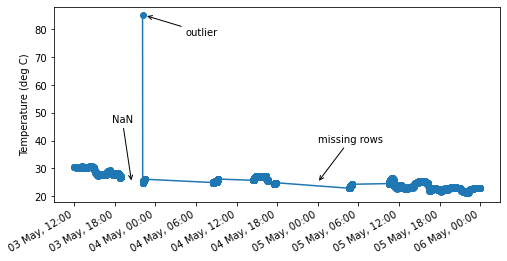
\includegraphics{outliers/temp-outlier.png}

While most measured points are between 20 and 30 °C, there is obviously
something very wrong with the one data point above 80 °C.

How could such a thing come about? This could be the result of
\textbf{non-natural causes}, such as measurement errors, wrong data
collection, or wrong data entry. On the other hand, this point could
have \textbf{natural} sources, such as a very hot spark flying next to
the temperature sensor.

Identifying outliers is important, because they might greatly impact
measures like mean and standard deviation. When left untouched, outliers
might make us reach wrong conclusions about our data. See what happens
to the slope of this linear regression with and without the outliers.

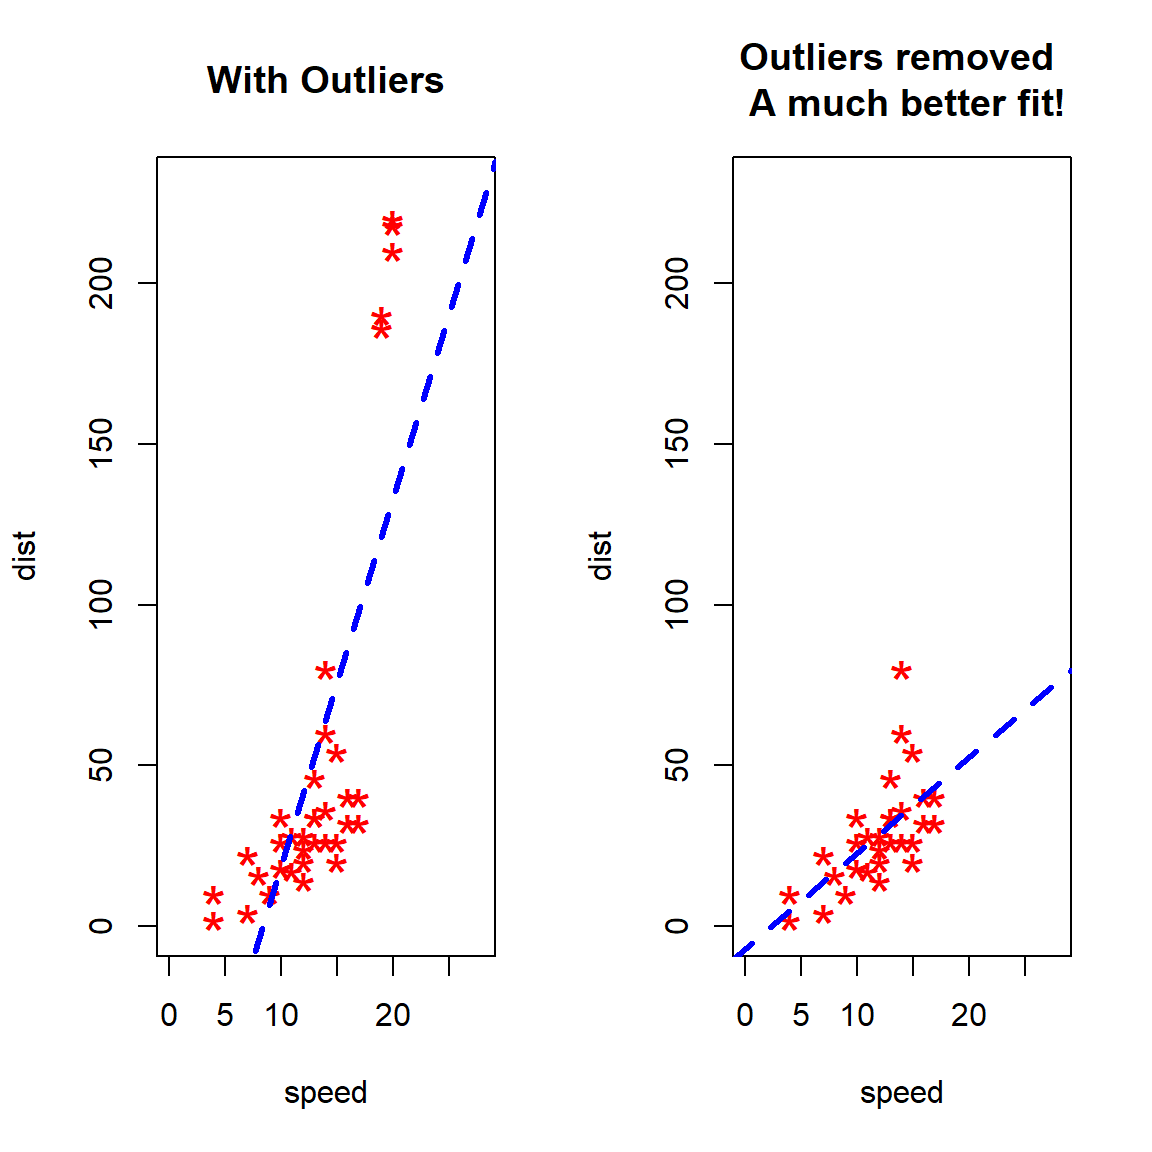
\includegraphics{outliers/regression-outlier.png}

\marginnote{\begin{footnotesize}

Source: Zhang (2020)

\end{footnotesize}}

\hypertarget{outlier-identification}{%
\chapter{outlier identification}\label{outlier-identification}}

\hypertarget{visual-inspection}{%
\section{visual inspection}\label{visual-inspection}}

I produced a stationary signal and added to it a few ouliers. Can you
tell where just by looking at the graph?
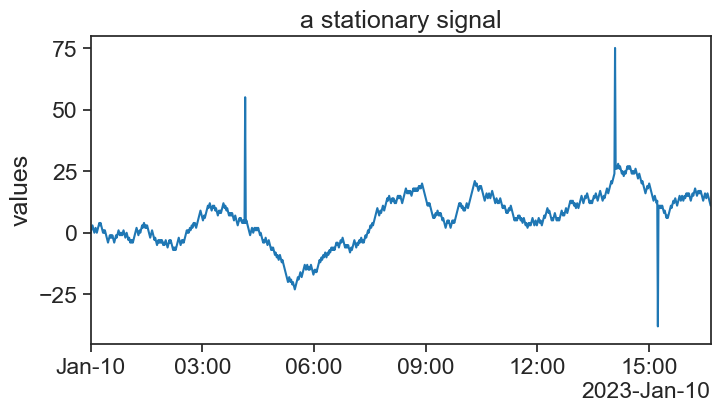
\includegraphics{outliers/signal_39_stationary.png}

The easiest way of identifying the outliers is:

\begin{itemize}
\tightlist
\item
  First plot the time series.
\item
  Choose upper and lower boundaries. Whatever falls outside these
  boundaries is an outlier.
\end{itemize}

Easy.

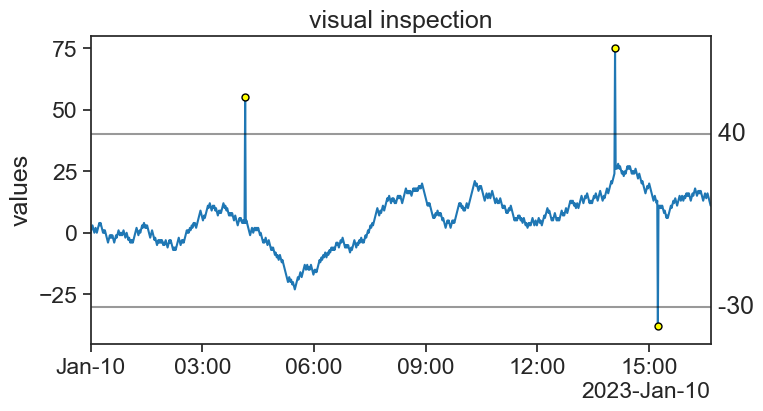
\includegraphics{outliers/outliers_visual_inspection.png}

If all you have is this one time series, you're done, congratulations.
However, it is often the case that one has very long time series, or a
great number of time series to analyze. In this case it is impractical
to use the visual inspection method. We would like to devise an
algorithm to automate this task.

\hypertarget{z-score}{%
\section{Z-score}\label{z-score}}

The Z-score is the distance, in units of 1 standard deviation, of a
point in the series with respect to the mean:

\[
z  = \frac{x-\mu}{\sigma},
\]

\marginnote{\begin{footnotesize}

where

\begin{itemize}
\tightlist
\item
  \(x=\) data point,\\
\item
  \(\mu=\) time series mean\\
\item
  \(\sigma=\) time series standard deviation.
\end{itemize}

\end{footnotesize}}

A common choice is to consider an outlier a point whose Z-score is
greater that 3, in absolute value. In other words: If a point is more
than 3 standard deviations away form the mean, then we call it an
outlier.

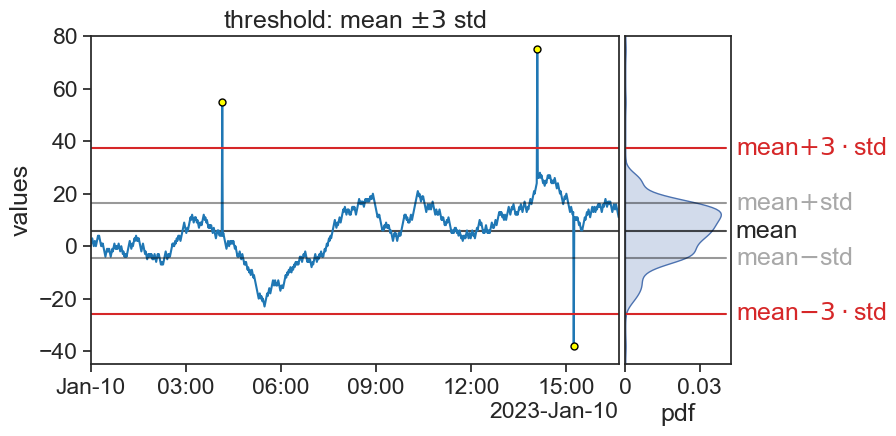
\includegraphics{outliers/outliers_3sigma.png}

You can now use this algorithm to any number of time series, let the
computer do the hard work.

Of course, there is nothing sacred about the number 3. You can choose
any Z-score you want to perform an analysis on your own data, depending
on your needs.

\hypertarget{attention}{%
\subsection{ATTENTION!}\label{attention}}

For data that is gaussianly distributed, we expect that 99.73\% of data
to fall within 3 standard deviations from the mean. In other words,
0.27\% of points would be considered as \emph{outliers} according to the
Z-score method.

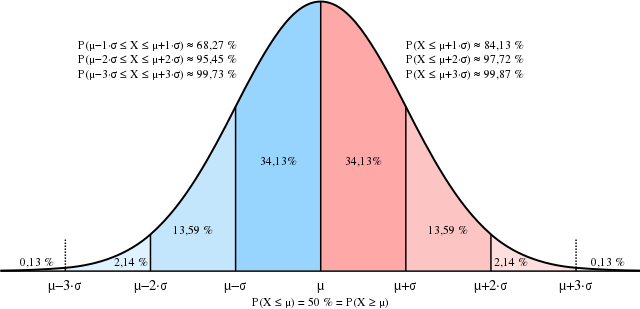
\includegraphics{outliers/Normal_Distribution_Sigma.png}

\marginnote{\begin{footnotesize}

Source:
\href{https://commons.wikimedia.org/wiki/File:Normal_Distribution_Sigma.svg}{Wikimedia
Commons}

\end{footnotesize}}

Assume you have a time series gaussianly distributed, with 10k
measurements. We would expect to find about 27 outliers in this time
series.

So what is the problem?!

The thing is, outliers are not supposed to be only data points far from
the other points. That's not enough. A better way of understanding
outliers is to imagine that our expected measurements are sampled from a
given distribution, and every now an then we have measurements that are
sampled from \textbf{another} distribution.

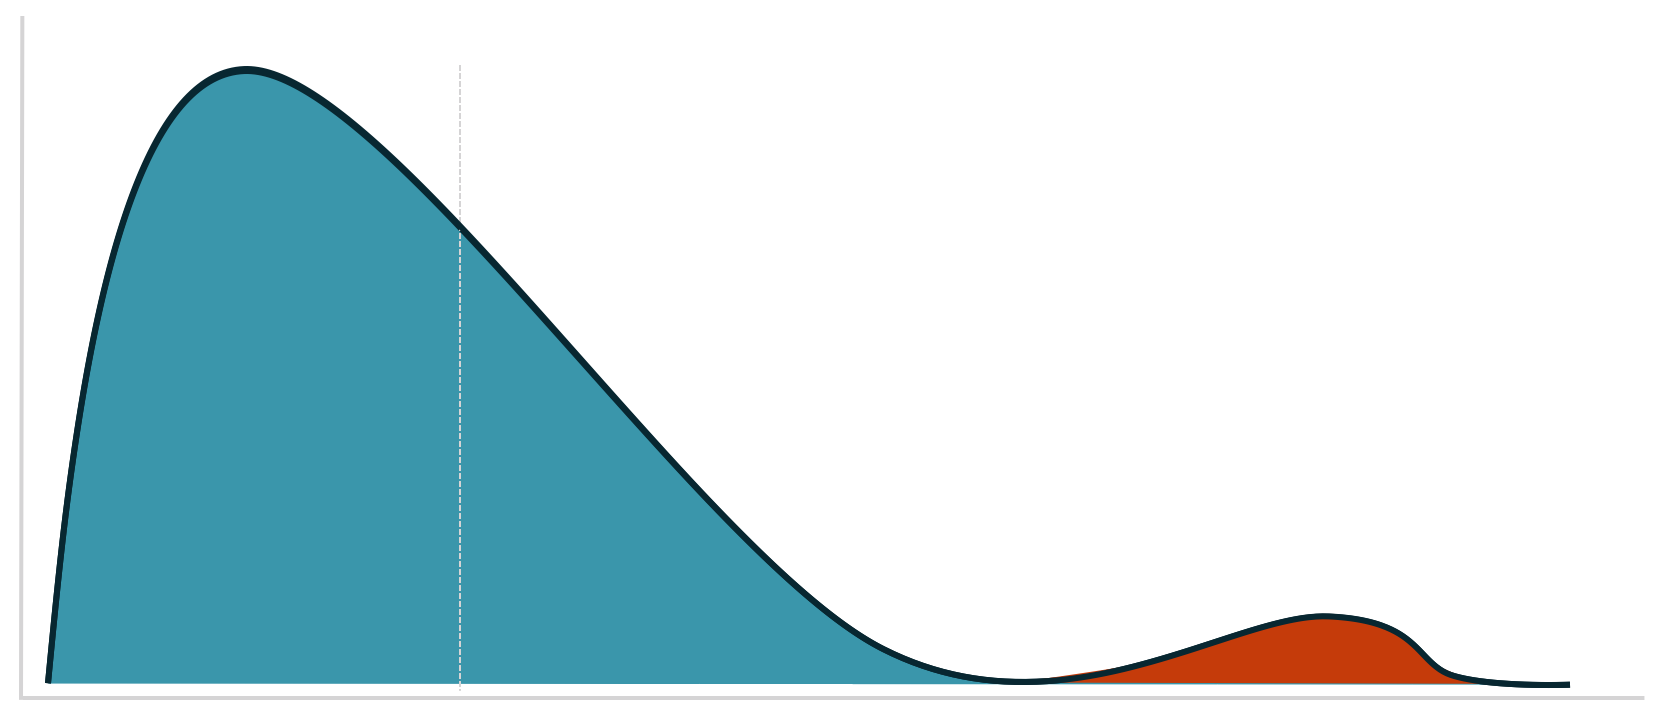
\includegraphics{outliers/two-distributions.png}

\marginnote{\begin{footnotesize}

Source:
\href{https://www.brooksbell.com/resource/blog/dealing-with-outliers-part-1/}{Taylor
Wilson's ``Dealing with Outliers (Part 1): Ignore Them at Your Peril''}

\end{footnotesize}}

We should have this in mind always. We wouldn't want to single out good
data as something weird. Our true task is to identify which points in
our time series were sampled from a different distribution. This can be
a very challenging task.

\hypertarget{iqr}{%
\section{IQR}\label{iqr}}

Another super common criterion for identifying outliers is the IQR, or
InterQuartile Range.

Take a look at the statistics below of the time series we have been
working with so far. The IQR is the distance between the first quartile
(Q1) and the third quartile (Q3), where exactly 50\% of the data is.

The algorithm here is to determine two thresholds, whose distance is 1.5
times the IQR from Q1 and Q3. Whatever falls outside these two
thresholds is an outlier.

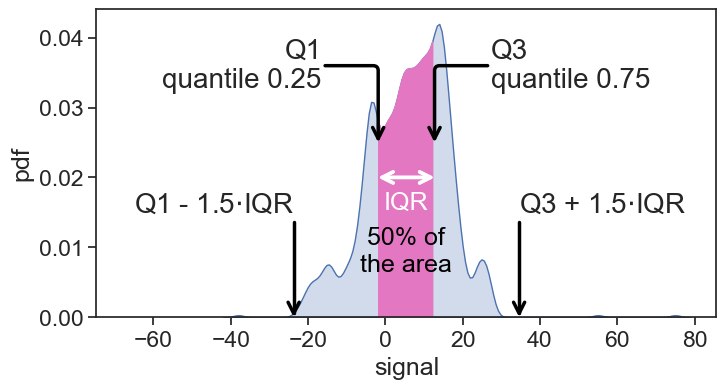
\includegraphics{outliers/IQR_pdf.png}

We are used to see this in box plots:

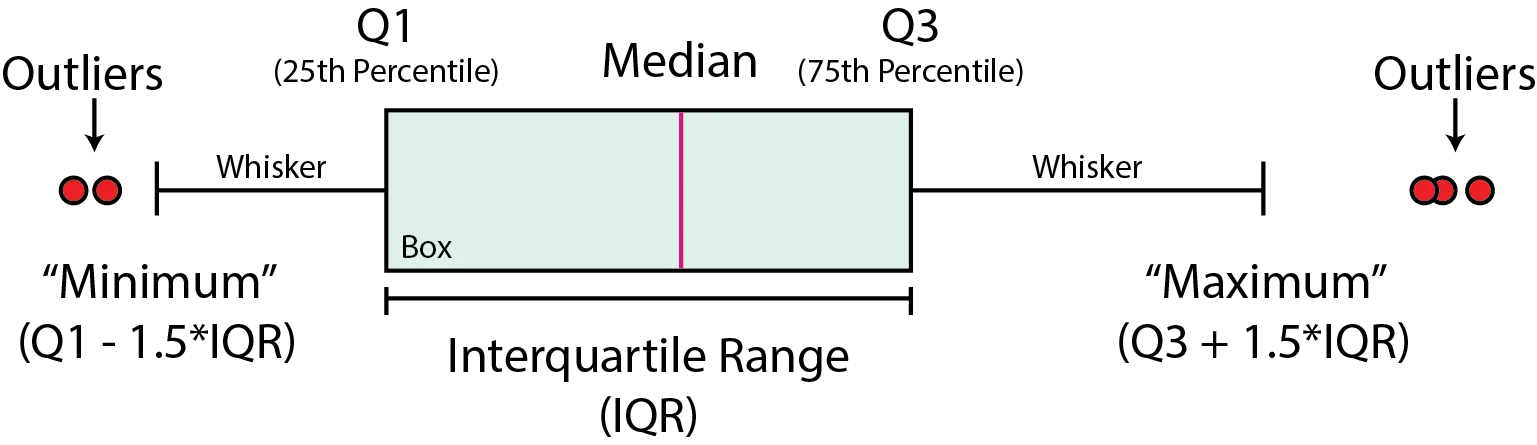
\includegraphics{outliers/iqr1.png}

\marginnote{\begin{footnotesize}

Source: McDonald (2022)

\end{footnotesize}}

Again, the distance 1.5 is not sacred, it's only the most common. You
might want to choose other values depending on your needs. Let's now
apply the IQR method to our time series.

\includegraphics{outliers/outliers_1.5IQR.png}

It works pretty well! Notice that now we have an additional outlier (a
bit before 06:00). What do we do with that?

\hypertarget{non-stationary-time-series}{%
\section{non-stationary time series}\label{non-stationary-time-series}}

I have produced a new time series, one that on average goes up with
time. Can you point in the graph where are the outliers?

\includegraphics{outliers/signal_40_non_stationary.png}

Now, see what happens when we apply the previous two methods to this
time series.

\textbf{Z-score}

\includegraphics{outliers/outliers_3sigma_seed40.png}

\textbf{IQR}

\includegraphics{outliers/outliers_1.5IQR_seed40.png}

What happened? Do you have ideas how to solve this?

\hypertarget{sources}{%
\section{Sources}\label{sources}}

\hypertarget{robust-analysis}{%
\chapter{robust analysis}\label{robust-analysis}}

A tool is said to be \textbf{robust} if outliers don't influence (much)
its results.

The average and standard deviation are \textbf{not} robust.

\begin{Shaded}
\begin{Highlighting}[]
\ImportTok{import}\NormalTok{ numpy }\ImportTok{as}\NormalTok{ np}
\NormalTok{series1 }\OperatorTok{=}\NormalTok{ np.array([}\DecValTok{0}\NormalTok{, }\DecValTok{1}\NormalTok{, }\DecValTok{2}\NormalTok{, }\DecValTok{3}\NormalTok{, }\DecValTok{4}\NormalTok{, }\DecValTok{5}\NormalTok{, }\DecValTok{6}\NormalTok{])}
\NormalTok{series2 }\OperatorTok{=}\NormalTok{ np.array([}\DecValTok{0}\NormalTok{, }\DecValTok{1}\NormalTok{, }\DecValTok{2}\NormalTok{, }\DecValTok{3}\NormalTok{, }\DecValTok{4}\NormalTok{, }\DecValTok{5}\NormalTok{, }\DecValTok{60}\NormalTok{])}
\BuiltInTok{print}\NormalTok{(}\SpecialStringTok{f"series 1: mean=}\SpecialCharTok{\{}\NormalTok{series1}\SpecialCharTok{.}\NormalTok{mean()}\SpecialCharTok{:.2f\}}\SpecialStringTok{, std=}\SpecialCharTok{\{}\NormalTok{series1}\SpecialCharTok{.}\NormalTok{std()}\SpecialCharTok{:.2f\}}\SpecialStringTok{"}\NormalTok{)}
\BuiltInTok{print}\NormalTok{(}\SpecialStringTok{f"series 2: mean=}\SpecialCharTok{\{}\NormalTok{series2}\SpecialCharTok{.}\NormalTok{mean()}\SpecialCharTok{:.2f\}}\SpecialStringTok{, std=}\SpecialCharTok{\{}\NormalTok{series2}\SpecialCharTok{.}\NormalTok{std()}\SpecialCharTok{:.2f\}}\SpecialStringTok{"}\NormalTok{)}
\end{Highlighting}
\end{Shaded}

\begin{verbatim}
series 1: mean=3.00, std=2.00
series 2: mean=10.71, std=20.18
\end{verbatim}

On the other hand, the median and IQR are robust:

\begin{Shaded}
\begin{Highlighting}[]
\ImportTok{from}\NormalTok{ scipy.stats }\ImportTok{import}\NormalTok{ iqr}
\BuiltInTok{print}\NormalTok{(}\SpecialStringTok{f"series 1: median=}\SpecialCharTok{\{}\NormalTok{np}\SpecialCharTok{.}\NormalTok{median(series1)}\SpecialCharTok{:.2f\}}\SpecialStringTok{, IQR=}\SpecialCharTok{\{}\NormalTok{iqr(series1)}\SpecialCharTok{:.2f\}}\SpecialStringTok{"}\NormalTok{)}
\BuiltInTok{print}\NormalTok{(}\SpecialStringTok{f"series 2: median=}\SpecialCharTok{\{}\NormalTok{np}\SpecialCharTok{.}\NormalTok{median(series2)}\SpecialCharTok{:.2f\}}\SpecialStringTok{, IQR=}\SpecialCharTok{\{}\NormalTok{iqr(series2)}\SpecialCharTok{:.2f\}}\SpecialStringTok{"}\NormalTok{)}
\end{Highlighting}
\end{Shaded}

\begin{verbatim}
series 1: median=3.00, IQR=3.00
series 2: median=3.00, IQR=3.00
\end{verbatim}

\hypertarget{mad}{%
\section{MAD}\label{mad}}

Another rubust method is MAD, the Median Absolute Deviation, given by

\[
\text{MAD} = \text{median}(\left| x_i - \text{median}(x)  \right|),
\]

where \(|\cdot|\) is the absolute value.

Applying MAD to the stationary time series from before, yields

\includegraphics{outliers/outliers_MAD_stationary.png}

Here, the threshold is the median \(\pm3k\cdot\) MAD, where the value
\(k=1.4826\) scales MAD so that when the data is gaussianly distributed,
\(3k\) equals 1 standard deviation.

\hypertarget{sliding-algorithms}{%
\chapter{sliding algorithms}\label{sliding-algorithms}}

None of the methods learned before seem appropriate to deal with
non-stationary data. A simple solution is to apply those methods for
sliding windows of ``appropriate'' widths.

\hypertarget{sliding-z-score}{%
\section{Sliding Z-score}\label{sliding-z-score}}

\includegraphics{outliers/outliers_rolling_3std.png}

Now the Z-score seems to give really nice results (but not perfect).
Maybe playing with the window width and Z-score threshold would give
better results?

In any case, we clearly see why the Z-score is not a robust algorithm.
See how the standard deviation is sensitive to outliers?

\hypertarget{sliding-iqr}{%
\section{Sliding IQR}\label{sliding-iqr}}

Let's see how well the sliding IQR method fares.

\includegraphics{outliers/outliers_rolling_IQR.png}

It identified all the outliers, but also found that a few \emph{other}
points should be considered outliers? What do you think of that?

See that the threshold does not jump abruptly when the sliding window
includes an outlier. In fact, the threshold doesn't even care! This is
what it means to be robust.

However, we do see large fluctuations in the threshold. When does this
happen? Why?

\hypertarget{sliding-mad}{%
\section{Sliding MAD}\label{sliding-mad}}

Now it's MAD's time to shine.

\includegraphics{outliers/outliers_rolling_MAD.png}

Compare this result to the previous two. Which yields best results?

MAD is robust to outliers, and again we see that the threshold envelope
widens when there is a rising or falling trend in the data.

\hypertarget{challenges-1}{%
\section{Challenges}\label{challenges-1}}

Now it's your turn to work, I'm tired! Write algorithms for the
following outlier identification methods:

\begin{enumerate}
\def\labelenumi{\arabic{enumi}.}
\tightlist
\item
  visual inspection
\item
  Z-score
\item
  IQR
\item
  MAD
\end{enumerate}

Excluding the visual inspection method, write first an algorithm that
operates on a full time series, and then write a new version that can
work with sliding windows.

\hypertarget{substituting-outliers}{%
\chapter{substituting outliers}\label{substituting-outliers}}

Ok. We found the outliers. Now what?!

As usual, it depends.

\hypertarget{do-nothing}{%
\section{Do nothing}\label{do-nothing}}

Assuming the outlier indeed happened in real life, and is not the result
of faulty data transmission or bad data recording, then excluding an
outlier might be the last thing you want to do. Sometimes extreme events
do happen, such as a one-in-a-hundred-year storm, and they have a
disproportionate weight on the system you are studying. The outliers
might actually be the most interesting points in your data for all you
know!

In case the outliers are not of interest to you, if you are using
\textbf{robust} methods to analyze your data, you don't necessarily need
to do anything either. For instance, let's say that you want to smooth
your time series. If instead of taking the \texttt{mean} inside a
sliding window you choose to calculate the \texttt{median}, then
outliers shouldn't be a problem. Test it and see if it's true. Go on.

For many things you need to do (not only smoothing), you might be able
to find robust methods. What do you do if you \textbf{have} to use a
non-robust method? Well, then you can substitute the outlier for two
things: NaN or imputated values.

\hypertarget{nan}{%
\section{NaN}\label{nan}}

Substitute outliers for NaN.

NaN means ``Not a Number'', and is what you get when you try to perform
a mathematical operation like 0/0. It is common to see NaN in dataset
rows when data was not collected for some reason.

This might seem like a neutral solution, but it actually can generate
problems down the line. See this example:

\begin{Shaded}
\begin{Highlighting}[]
\ImportTok{import}\NormalTok{ numpy }\ImportTok{as}\NormalTok{ np}
\ImportTok{import}\NormalTok{ pandas }\ImportTok{as}\NormalTok{ pd}
\ImportTok{import}\NormalTok{ matplotlib.pyplot }\ImportTok{as}\NormalTok{ plt}
\ImportTok{from}\NormalTok{ matplotlib.dates }\ImportTok{import}\NormalTok{ DateFormatter}
\ImportTok{import}\NormalTok{ matplotlib.dates }\ImportTok{as}\NormalTok{ mdates}
\ImportTok{import}\NormalTok{ seaborn }\ImportTok{as}\NormalTok{ sns}
\NormalTok{sns.}\BuiltInTok{set}\NormalTok{(style}\OperatorTok{=}\StringTok{"ticks"}\NormalTok{, font\_scale}\OperatorTok{=}\FloatTok{1.5}\NormalTok{)  }\CommentTok{\# white graphs, with large and legible letters}
\ImportTok{from}\NormalTok{ scipy.signal }\ImportTok{import}\NormalTok{ savgol\_filter}
\end{Highlighting}
\end{Shaded}

\begin{Shaded}
\begin{Highlighting}[]
\CommentTok{\# example using numpy}
\NormalTok{series }\OperatorTok{=}\NormalTok{ np.array([}\DecValTok{2}\NormalTok{, }\DecValTok{4}\NormalTok{, }\DecValTok{5}\NormalTok{, np.nan, }\DecValTok{8}\NormalTok{, }\DecValTok{15}\NormalTok{])}
\NormalTok{mean }\OperatorTok{=}\NormalTok{ np.mean(series)}
\BuiltInTok{print}\NormalTok{(}\SpecialStringTok{f"the series average is }\SpecialCharTok{\{}\NormalTok{mean}\SpecialCharTok{\}}\SpecialStringTok{"}\NormalTok{)}
\end{Highlighting}
\end{Shaded}

\begin{verbatim}
the series average is nan
\end{verbatim}

A single NaN in your time series ruins the whole calculation! There is a
workaround though:

\begin{Shaded}
\begin{Highlighting}[]
\NormalTok{mean }\OperatorTok{=}\NormalTok{ np.nanmean(series)}
\BuiltInTok{print}\NormalTok{(}\SpecialStringTok{f"the series average is }\SpecialCharTok{\{}\NormalTok{mean}\SpecialCharTok{\}}\SpecialStringTok{"}\NormalTok{)}
\end{Highlighting}
\end{Shaded}

\begin{verbatim}
the series average is 6.8
\end{verbatim}

You have to make sure what is the behavior of each function you use with
respect to NaNs, and if possible, use a suitable substitute.

The same example in \texttt{pandas} would not fail:

\begin{Shaded}
\begin{Highlighting}[]
\NormalTok{date\_range }\OperatorTok{=}\NormalTok{ pd.date\_range(start}\OperatorTok{=}\StringTok{\textquotesingle{}2024{-}01{-}01\textquotesingle{}}\NormalTok{, periods}\OperatorTok{=}\BuiltInTok{len}\NormalTok{(series), freq}\OperatorTok{=}\StringTok{\textquotesingle{}1D\textquotesingle{}}\NormalTok{)}
\NormalTok{df }\OperatorTok{=}\NormalTok{ pd.DataFrame(\{}\StringTok{\textquotesingle{}series\textquotesingle{}}\NormalTok{: series\}, index}\OperatorTok{=}\NormalTok{date\_range)}
\NormalTok{mean }\OperatorTok{=}\NormalTok{ df[}\StringTok{\textquotesingle{}series\textquotesingle{}}\NormalTok{].mean()}
\BuiltInTok{print}\NormalTok{(}\SpecialStringTok{f"the series average is }\SpecialCharTok{\{}\NormalTok{mean}\SpecialCharTok{\}}\SpecialStringTok{"}\NormalTok{)}
\end{Highlighting}
\end{Shaded}

\begin{verbatim}
the series average is 6.8
\end{verbatim}

\hypertarget{imputate-values}{%
\section{imputate values}\label{imputate-values}}

To ``imputate values'' means to fill in the missing value with a guess,
an estimation of what this data point ``should have been'' if it were
measured in the first place. Why should we bother to do so? Because many
tools that we know and love don't do well with missing values.

We learned about the Savitzky-Golay filter for smoothing data. See what
happens when there is a single NaN in the series:

\begin{Shaded}
\begin{Highlighting}[]
\NormalTok{steps }\OperatorTok{=}\NormalTok{ np.random.randint(low}\OperatorTok{={-}}\DecValTok{2}\NormalTok{, high}\OperatorTok{=}\DecValTok{2}\NormalTok{, size}\OperatorTok{=}\DecValTok{100}\NormalTok{)}
\NormalTok{data }\OperatorTok{=}\NormalTok{ steps.cumsum()}
\NormalTok{date\_range }\OperatorTok{=}\NormalTok{ pd.date\_range(start}\OperatorTok{=}\StringTok{\textquotesingle{}2023{-}01{-}01\textquotesingle{}}\NormalTok{, periods}\OperatorTok{=}\BuiltInTok{len}\NormalTok{(data), freq}\OperatorTok{=}\StringTok{\textquotesingle{}1D\textquotesingle{}}\NormalTok{)}
\NormalTok{df }\OperatorTok{=}\NormalTok{ pd.DataFrame(\{}\StringTok{\textquotesingle{}series\textquotesingle{}}\NormalTok{: data\}, index}\OperatorTok{=}\NormalTok{date\_range)}
\NormalTok{df.loc[}\StringTok{\textquotesingle{}2023{-}02{-}05\textquotesingle{}}\NormalTok{, }\StringTok{\textquotesingle{}series\textquotesingle{}}\NormalTok{] }\OperatorTok{=}\NormalTok{ np.nan}
\end{Highlighting}
\end{Shaded}

\begin{Shaded}
\begin{Highlighting}[]
\NormalTok{df[}\StringTok{\textquotesingle{}sg\textquotesingle{}}\NormalTok{] }\OperatorTok{=}\NormalTok{ savgol\_filter(df[}\StringTok{\textquotesingle{}series\textquotesingle{}}\NormalTok{], window\_length}\OperatorTok{=}\DecValTok{15}\NormalTok{, polyorder}\OperatorTok{=}\DecValTok{2}\NormalTok{)}

\KeywordTok{def}\NormalTok{ concise(ax):}
\NormalTok{    locator }\OperatorTok{=}\NormalTok{ mdates.AutoDateLocator(minticks}\OperatorTok{=}\DecValTok{3}\NormalTok{, maxticks}\OperatorTok{=}\DecValTok{7}\NormalTok{)}
\NormalTok{    formatter }\OperatorTok{=}\NormalTok{ mdates.ConciseDateFormatter(locator)}
\NormalTok{    ax.xaxis.set\_major\_locator(locator)}
\NormalTok{    ax.xaxis.set\_major\_formatter(formatter)}

\NormalTok{fig, ax }\OperatorTok{=}\NormalTok{ plt.subplots(figsize}\OperatorTok{=}\NormalTok{(}\DecValTok{8}\NormalTok{,}\DecValTok{4}\NormalTok{))}
\NormalTok{ax.plot(df[}\StringTok{\textquotesingle{}series\textquotesingle{}}\NormalTok{], color}\OperatorTok{=}\StringTok{"tab:blue"}\NormalTok{, label}\OperatorTok{=}\StringTok{"series with 1 NaN"}\NormalTok{)}
\NormalTok{ax.plot(df[}\StringTok{\textquotesingle{}sg\textquotesingle{}}\NormalTok{], color}\OperatorTok{=}\StringTok{"tab:orange"}\NormalTok{, label}\OperatorTok{=}\StringTok{"SavGol filter has many more NaNs"}\NormalTok{)}
\NormalTok{concise(ax)}
\NormalTok{ax.legend(frameon}\OperatorTok{=}\VariableTok{False}\NormalTok{)}\OperatorTok{;}
\end{Highlighting}
\end{Shaded}

\begin{figure}[H]

{\centering \includegraphics{outliers/substituting-outliers_files/figure-pdf/cell-7-output-1.png}

}

\end{figure}

We will deal with this topic in the next chapter, ``interpolation''.
There, we will learn a few methods to fill in missing data, and basic
NaN operations you should be acquainted with.

\hypertarget{challenge}{%
\chapter{challenge}\label{challenge}}

\hypertarget{importing-bad-.csv-files}{%
\section{importing bad .csv files}\label{importing-bad-.csv-files}}

Here we will get a taste of what it feels like to work with bad
\texttt{.csv} files and how to fix them.

TO DO:

\begin{enumerate}
\def\labelenumi{\arabic{enumi}.}
\tightlist
\item
  create a folder for this challenge, name it whatever you want.
\item
  downlad this jupyter notebook and move to that folder.
\item
  download these 3 \texttt{.csv} files and part 2 notebook:

  \begin{enumerate}
  \def\labelenumii{\arabic{enumii}.}
  \tightlist
  \item
    cleaning1
  \item
    cleaning2-
  \item
    cleaning3
  \item
    part\_2
  \end{enumerate}
\item
  move them files into your folder
\end{enumerate}

\hypertarget{import}{%
\subsection{import}\label{import}}

\begin{Shaded}
\begin{Highlighting}[]
\ImportTok{import}\NormalTok{ pandas }\ImportTok{as}\NormalTok{ pd}
\ImportTok{import}\NormalTok{ numpy }\ImportTok{as}\NormalTok{ np}
\ImportTok{import}\NormalTok{ matplotlib.pyplot }\ImportTok{as}\NormalTok{ plt}
\ImportTok{from}\NormalTok{ matplotlib.dates }\ImportTok{import}\NormalTok{ DateFormatter}
\ImportTok{import}\NormalTok{ matplotlib.dates }\ImportTok{as}\NormalTok{ mdates}
\ImportTok{import}\NormalTok{ matplotlib.ticker }\ImportTok{as}\NormalTok{ ticker}
\ImportTok{import}\NormalTok{ warnings}
\CommentTok{\# Suppress FutureWarnings}
\NormalTok{warnings.simplefilter(action}\OperatorTok{=}\StringTok{\textquotesingle{}ignore\textquotesingle{}}\NormalTok{, category}\OperatorTok{=}\PreprocessorTok{FutureWarning}\NormalTok{)}
\NormalTok{warnings.simplefilter(action}\OperatorTok{=}\StringTok{\textquotesingle{}ignore\textquotesingle{}}\NormalTok{, category}\OperatorTok{=}\PreprocessorTok{UserWarning}\NormalTok{)}
\ImportTok{import}\NormalTok{ seaborn }\ImportTok{as}\NormalTok{ sns}
\NormalTok{sns.}\BuiltInTok{set}\NormalTok{(style}\OperatorTok{=}\StringTok{"ticks"}\NormalTok{, font\_scale}\OperatorTok{=}\FloatTok{1.5}\NormalTok{)  }\CommentTok{\# white graphs, with large and legible letters}

\CommentTok{\# \%matplotlib widget}
\end{Highlighting}
\end{Shaded}

\hypertarget{dataset-1}{%
\section{dataset 1:}\label{dataset-1}}

\begin{Shaded}
\begin{Highlighting}[]
\NormalTok{df1 }\OperatorTok{=}\NormalTok{ pd.read\_csv(}\StringTok{\textquotesingle{}cleaning1.csv\textquotesingle{}}\NormalTok{)}
\NormalTok{df1}
\end{Highlighting}
\end{Shaded}

\begin{longtable}[]{@{}lllllll@{}}
\toprule\noalign{}
& date & A & B & C & D & E \\
\midrule\noalign{}
\endhead
\bottomrule\noalign{}
\endlastfoot
0 & 2023-01-01 00:00:00 & 0 & 0.000000 & 0.000000 & 0.000000 &
0.000000 \\
1 & 2023-01-01 00:05:00 & 1 & 2.245251 & -1.757193 & 1.899602 &
-0.999300 \\
2 & 2023-01-01 00:10:00 & 2 & 2.909648 & 0.854732 & 2.050146 &
-0.559504 \\
3 & 2023-01-01 00:15:00 & 3 & 3.483155 & 0.946937 & 1.921080 &
-0.402084 \\
4 & 2023-01-01 00:20:00 & 2 & 4.909169 & 0.462239 & 1.368470 &
-0.698579 \\
... & ... & ... & ... & ... & ... & ... \\
105115 & 2023-12-31 23:35:00 & -37 & 1040.909898 & -14808.285199 &
1505.020266 & 423.595984 \\
105116 & 2023-12-31 23:40:00 & -36 & 1040.586547 & -14808.874072 &
1503.915566 & 423.117110 \\
105117 & 2023-12-31 23:45:00 & -37 & 1042.937417 & -14808.690745 &
1505.479671 & 423.862810 \\
105118 & 2023-12-31 23:50:00 & -36 & 1042.411572 & -14809.212002 &
1506.174334 & 423.862432 \\
105119 & 2023-12-31 23:55:00 & -35 & 1043.053520 & -14809.990338 &
1505.767197 & 423.647007 \\
\end{longtable}

Now let's put the column `date' in the index with datetime format

\begin{Shaded}
\begin{Highlighting}[]
\CommentTok{\# we can change the format of the column to datetime and then set it as the index.}
\NormalTok{df1[}\StringTok{\textquotesingle{}date\textquotesingle{}}\NormalTok{] }\OperatorTok{=}\NormalTok{ pd.to\_datetime(df1[}\StringTok{\textquotesingle{}date\textquotesingle{}}\NormalTok{])}
\NormalTok{df1.set\_index(}\StringTok{\textquotesingle{}date\textquotesingle{}}\NormalTok{, inplace}\OperatorTok{=}\VariableTok{True}\NormalTok{)}
\NormalTok{df1}
\end{Highlighting}
\end{Shaded}

\begin{longtable}[]{@{}llllll@{}}
\toprule\noalign{}
& A & B & C & D & E \\
date & & & & & \\
\midrule\noalign{}
\endhead
\bottomrule\noalign{}
\endlastfoot
2023-01-01 00:00:00 & 0 & 0.000000 & 0.000000 & 0.000000 & 0.000000 \\
2023-01-01 00:05:00 & 1 & 2.245251 & -1.757193 & 1.899602 & -0.999300 \\
2023-01-01 00:10:00 & 2 & 2.909648 & 0.854732 & 2.050146 & -0.559504 \\
2023-01-01 00:15:00 & 3 & 3.483155 & 0.946937 & 1.921080 & -0.402084 \\
2023-01-01 00:20:00 & 2 & 4.909169 & 0.462239 & 1.368470 & -0.698579 \\
... & ... & ... & ... & ... & ... \\
2023-12-31 23:35:00 & -37 & 1040.909898 & -14808.285199 & 1505.020266 &
423.595984 \\
2023-12-31 23:40:00 & -36 & 1040.586547 & -14808.874072 & 1503.915566 &
423.117110 \\
2023-12-31 23:45:00 & -37 & 1042.937417 & -14808.690745 & 1505.479671 &
423.862810 \\
2023-12-31 23:50:00 & -36 & 1042.411572 & -14809.212002 & 1506.174334 &
423.862432 \\
2023-12-31 23:55:00 & -35 & 1043.053520 & -14809.990338 & 1505.767197 &
423.647007 \\
\end{longtable}

If we know that in advance so we can do all of that when we import the
csv

\begin{Shaded}
\begin{Highlighting}[]
\NormalTok{df1 }\OperatorTok{=}\NormalTok{ pd.read\_csv(}\StringTok{\textquotesingle{}cleaning1.csv\textquotesingle{}}\NormalTok{, }
\NormalTok{                  index\_col}\OperatorTok{=}\StringTok{\textquotesingle{}date\textquotesingle{}}\NormalTok{,     }\CommentTok{\# set the column date as index }
\NormalTok{                  parse\_dates}\OperatorTok{=}\VariableTok{True}\NormalTok{)     }\CommentTok{\# turn to datetime format}
\NormalTok{df1}
\end{Highlighting}
\end{Shaded}

\begin{longtable}[]{@{}llllll@{}}
\toprule\noalign{}
& A & B & C & D & E \\
date & & & & & \\
\midrule\noalign{}
\endhead
\bottomrule\noalign{}
\endlastfoot
2023-01-01 00:00:00 & 0 & 0.000000 & 0.000000 & 0.000000 & 0.000000 \\
2023-01-01 00:05:00 & 1 & 2.245251 & -1.757193 & 1.899602 & -0.999300 \\
2023-01-01 00:10:00 & 2 & 2.909648 & 0.854732 & 2.050146 & -0.559504 \\
2023-01-01 00:15:00 & 3 & 3.483155 & 0.946937 & 1.921080 & -0.402084 \\
2023-01-01 00:20:00 & 2 & 4.909169 & 0.462239 & 1.368470 & -0.698579 \\
... & ... & ... & ... & ... & ... \\
2023-12-31 23:35:00 & -37 & 1040.909898 & -14808.285199 & 1505.020266 &
423.595984 \\
2023-12-31 23:40:00 & -36 & 1040.586547 & -14808.874072 & 1503.915566 &
423.117110 \\
2023-12-31 23:45:00 & -37 & 1042.937417 & -14808.690745 & 1505.479671 &
423.862810 \\
2023-12-31 23:50:00 & -36 & 1042.411572 & -14809.212002 & 1506.174334 &
423.862432 \\
2023-12-31 23:55:00 & -35 & 1043.053520 & -14809.990338 & 1505.767197 &
423.647007 \\
\end{longtable}

Now lets plot all the columns and see what we have

\begin{Shaded}
\begin{Highlighting}[]
\KeywordTok{def}\NormalTok{ plot\_all\_columns(data):}
\NormalTok{    column\_list }\OperatorTok{=}\NormalTok{ data.columns}
    
\NormalTok{    fig, ax }\OperatorTok{=}\NormalTok{ plt.subplots(}\BuiltInTok{len}\NormalTok{(column\_list),}\DecValTok{1}\NormalTok{, sharex}\OperatorTok{=}\VariableTok{True}\NormalTok{, figsize}\OperatorTok{=}\NormalTok{(}\DecValTok{10}\NormalTok{,}\BuiltInTok{len}\NormalTok{(column\_list)}\OperatorTok{*}\DecValTok{2}\NormalTok{))}

    \ControlFlowTok{if} \BuiltInTok{len}\NormalTok{(column\_list) }\OperatorTok{==} \DecValTok{1}\NormalTok{:}
\NormalTok{        ax.plot(data[column\_list[}\DecValTok{0}\NormalTok{]])}
        \ControlFlowTok{return}
    \ControlFlowTok{for}\NormalTok{ i, column }\KeywordTok{in} \BuiltInTok{enumerate}\NormalTok{(column\_list):}
\NormalTok{        ax[i].plot(data[column])}
\NormalTok{        ax[i].}\BuiltInTok{set}\NormalTok{(ylabel}\OperatorTok{=}\NormalTok{column)}
    
\NormalTok{    locator }\OperatorTok{=}\NormalTok{ mdates.AutoDateLocator(minticks}\OperatorTok{=}\DecValTok{3}\NormalTok{, maxticks}\OperatorTok{=}\DecValTok{7}\NormalTok{)}
\NormalTok{    formatter }\OperatorTok{=}\NormalTok{ mdates.ConciseDateFormatter(locator)}
\NormalTok{    ax[i].xaxis.set\_major\_locator(locator)}
\NormalTok{    ax[i].xaxis.set\_major\_formatter(formatter)}

    \ControlFlowTok{return}
\end{Highlighting}
\end{Shaded}

\begin{Shaded}
\begin{Highlighting}[]
\NormalTok{plot\_all\_columns(df1)}
\end{Highlighting}
\end{Shaded}

\begin{figure}[H]

{\centering \includegraphics{outliers/outliers_challenge_files/figure-pdf/cell-7-output-1.png}

}

\end{figure}

Looks like some of this data needs cleaning\ldots..

\hypertarget{dataset-2}{%
\section{Dataset 2:}\label{dataset-2}}

\begin{Shaded}
\begin{Highlighting}[]
\NormalTok{df2 }\OperatorTok{=}\NormalTok{ pd.read\_csv(}\StringTok{\textquotesingle{}cleaning2{-}.csv\textquotesingle{}}\NormalTok{)}
\NormalTok{df2}
\end{Highlighting}
\end{Shaded}

\begin{longtable}[]{@{}ll@{}}
\toprule\noalign{}
& A B date time \\
\midrule\noalign{}
\endhead
\bottomrule\noalign{}
\endlastfoot
0 & 0.0 0.0 01012023 00:00:00 \\
1 & -2.0275363548598184 0.011984922825112581 01012... \\
2 & -2.690616715983192 -0.29792822981957684 010120... \\
3 & -1.9859899758267612 -0.30940867922490206 01012... \\
4 & -2.290897621584889 -2.8666633353521624 0101202... \\
... & ... \\
8755 & -74.51464473079395 293.8680858227996 31122023 ... \\
8756 & -74.73805809332175 294.7593463919649 31122023 ... \\
8757 & -75.84842465358788 294.07634907736116 31122023... \\
8758 & -77.27218272637339 293.526461290973 31122023 2... \\
8759 & -76.55739976945038 293.35336890454107 31122023... \\
\end{longtable}

Something is wrong\ldots{}\\
lets open the actual \texttt{.csv} file and take a quick look.\\
It seems that the values are seperated by space and not by commas
\texttt{,}.

\begin{Shaded}
\begin{Highlighting}[]
\NormalTok{df2 }\OperatorTok{=}\NormalTok{ pd.read\_csv(}\StringTok{\textquotesingle{}cleaning2{-}.csv\textquotesingle{}}\NormalTok{, delimiter}\OperatorTok{=}\StringTok{\textquotesingle{} \textquotesingle{}}\NormalTok{)}
\NormalTok{df2}
\end{Highlighting}
\end{Shaded}

\begin{longtable}[]{@{}lllll@{}}
\toprule\noalign{}
& A & B & date & time \\
\midrule\noalign{}
\endhead
\bottomrule\noalign{}
\endlastfoot
0 & 0.000000 & 0.0 & 1012023 & 00:00:00 \\
1 & -2.027536 & 0.011984922825112581 & 1012023 & 01:00:00 \\
2 & -2.690617 & -0.29792822981957684 & 1012023 & 02:00:00 \\
3 & -1.985990 & -0.30940867922490206 & 1012023 & 03:00:00 \\
4 & -2.290898 & -2.8666633353521624 & 1012023 & 04:00:00 \\
... & ... & ... & ... & ... \\
8755 & -74.514645 & 293.8680858227996 & 31122023 & 19:00:00 \\
8756 & -74.738058 & 294.7593463919649 & 31122023 & 20:00:00 \\
8757 & -75.848425 & 294.07634907736116 & 31122023 & 21:00:00 \\
8758 & -77.272183 & 293.526461290973 & 31122023 & 22:00:00 \\
8759 & -76.557400 & 293.35336890454107 & 31122023 & 23:00:00 \\
\end{longtable}

\begin{Shaded}
\begin{Highlighting}[]
\CommentTok{\# convert the date column to datetime}
\NormalTok{df2[}\StringTok{\textquotesingle{}date\_corrected\textquotesingle{}}\NormalTok{] }\OperatorTok{=}\NormalTok{ pd.to\_datetime(df2[}\StringTok{\textquotesingle{}date\textquotesingle{}}\NormalTok{])}
\CommentTok{\# df2[\textquotesingle{}date\_corrected\textquotesingle{}] = pd.to\_datetime(df2[\textquotesingle{}date\textquotesingle{}], format=\textquotesingle{}\%d\%m\%Y\textquotesingle{})}

\NormalTok{df2}
\end{Highlighting}
\end{Shaded}

\begin{longtable}[]{@{}llllll@{}}
\toprule\noalign{}
& A & B & date & time & date\_corrected \\
\midrule\noalign{}
\endhead
\bottomrule\noalign{}
\endlastfoot
0 & 0.000000 & 0.0 & 1012023 & 00:00:00 & 1970-01-01
00:00:00.001012023 \\
1 & -2.027536 & 0.011984922825112581 & 1012023 & 01:00:00 & 1970-01-01
00:00:00.001012023 \\
2 & -2.690617 & -0.29792822981957684 & 1012023 & 02:00:00 & 1970-01-01
00:00:00.001012023 \\
3 & -1.985990 & -0.30940867922490206 & 1012023 & 03:00:00 & 1970-01-01
00:00:00.001012023 \\
4 & -2.290898 & -2.8666633353521624 & 1012023 & 04:00:00 & 1970-01-01
00:00:00.001012023 \\
... & ... & ... & ... & ... & ... \\
8755 & -74.514645 & 293.8680858227996 & 31122023 & 19:00:00 & 1970-01-01
00:00:00.031122023 \\
8756 & -74.738058 & 294.7593463919649 & 31122023 & 20:00:00 & 1970-01-01
00:00:00.031122023 \\
8757 & -75.848425 & 294.07634907736116 & 31122023 & 21:00:00 &
1970-01-01 00:00:00.031122023 \\
8758 & -77.272183 & 293.526461290973 & 31122023 & 22:00:00 & 1970-01-01
00:00:00.031122023 \\
8759 & -76.557400 & 293.35336890454107 & 31122023 & 23:00:00 &
1970-01-01 00:00:00.031122023 \\
\end{longtable}

\begin{Shaded}
\begin{Highlighting}[]
\CommentTok{\# df2[\textquotesingle{}date\_corrected\textquotesingle{}] = pd.to\_datetime(df2[\textquotesingle{}date\textquotesingle{}][:780], format=\textquotesingle{}\%d\%m\%Y\textquotesingle{})}
\CommentTok{\# df2[\textquotesingle{}date\_corrected\textquotesingle{}] = pd.to\_datetime(df2[\textquotesingle{}date\textquotesingle{}][780:800], format=\textquotesingle{}\%d\%m\%Y\textquotesingle{})}
\CommentTok{\# df2[\textquotesingle{}date\textquotesingle{}][780:800]}
\end{Highlighting}
\end{Shaded}

\begin{Shaded}
\begin{Highlighting}[]
\NormalTok{data\_types }\OperatorTok{=}\NormalTok{ \{}\StringTok{\textquotesingle{}date\textquotesingle{}}\NormalTok{: }\BuiltInTok{str}\NormalTok{ , }\StringTok{\textquotesingle{}time\textquotesingle{}}\NormalTok{:}\BuiltInTok{str}\NormalTok{\}}

\CommentTok{\# Read the CSV file with specified data types}
\NormalTok{df2 }\OperatorTok{=}\NormalTok{ pd.read\_csv(}\StringTok{\textquotesingle{}cleaning2{-}.csv\textquotesingle{}}\NormalTok{, delimiter}\OperatorTok{=}\StringTok{\textquotesingle{} \textquotesingle{}}\NormalTok{, dtype}\OperatorTok{=}\NormalTok{data\_types)}
\NormalTok{df2}
\end{Highlighting}
\end{Shaded}

\begin{longtable}[]{@{}lllll@{}}
\toprule\noalign{}
& A & B & date & time \\
\midrule\noalign{}
\endhead
\bottomrule\noalign{}
\endlastfoot
0 & 0.000000 & 0.0 & 01012023 & 00:00:00 \\
1 & -2.027536 & 0.011984922825112581 & 01012023 & 01:00:00 \\
2 & -2.690617 & -0.29792822981957684 & 01012023 & 02:00:00 \\
3 & -1.985990 & -0.30940867922490206 & 01012023 & 03:00:00 \\
4 & -2.290898 & -2.8666633353521624 & 01012023 & 04:00:00 \\
... & ... & ... & ... & ... \\
8755 & -74.514645 & 293.8680858227996 & 31122023 & 19:00:00 \\
8756 & -74.738058 & 294.7593463919649 & 31122023 & 20:00:00 \\
8757 & -75.848425 & 294.07634907736116 & 31122023 & 21:00:00 \\
8758 & -77.272183 & 293.526461290973 & 31122023 & 22:00:00 \\
8759 & -76.557400 & 293.35336890454107 & 31122023 & 23:00:00 \\
\end{longtable}

\begin{Shaded}
\begin{Highlighting}[]
\NormalTok{df2[}\StringTok{\textquotesingle{}date\_corrected\textquotesingle{}}\NormalTok{] }\OperatorTok{=}\NormalTok{ pd.to\_datetime(df2[}\StringTok{\textquotesingle{}date\textquotesingle{}}\NormalTok{], }\BuiltInTok{format}\OperatorTok{=}\StringTok{\textquotesingle{}}\SpecialCharTok{\%d}\StringTok{\%m\%Y\textquotesingle{}}\NormalTok{)}
\NormalTok{df2}
\end{Highlighting}
\end{Shaded}

\begin{longtable}[]{@{}llllll@{}}
\toprule\noalign{}
& A & B & date & time & date\_corrected \\
\midrule\noalign{}
\endhead
\bottomrule\noalign{}
\endlastfoot
0 & 0.000000 & 0.0 & 01012023 & 00:00:00 & 2023-01-01 \\
1 & -2.027536 & 0.011984922825112581 & 01012023 & 01:00:00 &
2023-01-01 \\
2 & -2.690617 & -0.29792822981957684 & 01012023 & 02:00:00 &
2023-01-01 \\
3 & -1.985990 & -0.30940867922490206 & 01012023 & 03:00:00 &
2023-01-01 \\
4 & -2.290898 & -2.8666633353521624 & 01012023 & 04:00:00 &
2023-01-01 \\
... & ... & ... & ... & ... & ... \\
8755 & -74.514645 & 293.8680858227996 & 31122023 & 19:00:00 &
2023-12-31 \\
8756 & -74.738058 & 294.7593463919649 & 31122023 & 20:00:00 &
2023-12-31 \\
8757 & -75.848425 & 294.07634907736116 & 31122023 & 21:00:00 &
2023-12-31 \\
8758 & -77.272183 & 293.526461290973 & 31122023 & 22:00:00 &
2023-12-31 \\
8759 & -76.557400 & 293.35336890454107 & 31122023 & 23:00:00 &
2023-12-31 \\
\end{longtable}

\begin{Shaded}
\begin{Highlighting}[]
\NormalTok{df2[}\StringTok{\textquotesingle{}datetime\textquotesingle{}}\NormalTok{] }\OperatorTok{=}\NormalTok{ pd.to\_datetime(df2[}\StringTok{\textquotesingle{}date\textquotesingle{}}\NormalTok{] }\OperatorTok{+} \StringTok{\textquotesingle{} \textquotesingle{}} \OperatorTok{+}\NormalTok{ df2[}\StringTok{\textquotesingle{}time\textquotesingle{}}\NormalTok{], }\BuiltInTok{format}\OperatorTok{=}\StringTok{\textquotesingle{}}\SpecialCharTok{\%d}\StringTok{\%m\%Y \%H:\%M:\%S\textquotesingle{}}\NormalTok{)}
\NormalTok{df2}
\end{Highlighting}
\end{Shaded}

\begin{longtable}[]{@{}lllllll@{}}
\toprule\noalign{}
& A & B & date & time & date\_corrected & datetime \\
\midrule\noalign{}
\endhead
\bottomrule\noalign{}
\endlastfoot
0 & 0.000000 & 0.0 & 01012023 & 00:00:00 & 2023-01-01 & 2023-01-01
00:00:00 \\
1 & -2.027536 & 0.011984922825112581 & 01012023 & 01:00:00 & 2023-01-01
& 2023-01-01 01:00:00 \\
2 & -2.690617 & -0.29792822981957684 & 01012023 & 02:00:00 & 2023-01-01
& 2023-01-01 02:00:00 \\
3 & -1.985990 & -0.30940867922490206 & 01012023 & 03:00:00 & 2023-01-01
& 2023-01-01 03:00:00 \\
4 & -2.290898 & -2.8666633353521624 & 01012023 & 04:00:00 & 2023-01-01 &
2023-01-01 04:00:00 \\
... & ... & ... & ... & ... & ... & ... \\
8755 & -74.514645 & 293.8680858227996 & 31122023 & 19:00:00 & 2023-12-31
& 2023-12-31 19:00:00 \\
8756 & -74.738058 & 294.7593463919649 & 31122023 & 20:00:00 & 2023-12-31
& 2023-12-31 20:00:00 \\
8757 & -75.848425 & 294.07634907736116 & 31122023 & 21:00:00 &
2023-12-31 & 2023-12-31 21:00:00 \\
8758 & -77.272183 & 293.526461290973 & 31122023 & 22:00:00 & 2023-12-31
& 2023-12-31 22:00:00 \\
8759 & -76.557400 & 293.35336890454107 & 31122023 & 23:00:00 &
2023-12-31 & 2023-12-31 23:00:00 \\
\end{longtable}

\begin{Shaded}
\begin{Highlighting}[]
\NormalTok{df2.drop(columns}\OperatorTok{=}\NormalTok{[}\StringTok{\textquotesingle{}date\textquotesingle{}}\NormalTok{, }\StringTok{\textquotesingle{}time\textquotesingle{}}\NormalTok{, }\StringTok{\textquotesingle{}date\_corrected\textquotesingle{}}\NormalTok{], inplace}\OperatorTok{=}\VariableTok{True}\NormalTok{)}
\NormalTok{df2.set\_index(}\StringTok{\textquotesingle{}datetime\textquotesingle{}}\NormalTok{, inplace}\OperatorTok{=}\VariableTok{True}\NormalTok{)}
\NormalTok{df2}
\end{Highlighting}
\end{Shaded}

\begin{longtable}[]{@{}lll@{}}
\toprule\noalign{}
& A & B \\
datetime & & \\
\midrule\noalign{}
\endhead
\bottomrule\noalign{}
\endlastfoot
2023-01-01 00:00:00 & 0.000000 & 0.0 \\
2023-01-01 01:00:00 & -2.027536 & 0.011984922825112581 \\
2023-01-01 02:00:00 & -2.690617 & -0.29792822981957684 \\
2023-01-01 03:00:00 & -1.985990 & -0.30940867922490206 \\
2023-01-01 04:00:00 & -2.290898 & -2.8666633353521624 \\
... & ... & ... \\
2023-12-31 19:00:00 & -74.514645 & 293.8680858227996 \\
2023-12-31 20:00:00 & -74.738058 & 294.7593463919649 \\
2023-12-31 21:00:00 & -75.848425 & 294.07634907736116 \\
2023-12-31 22:00:00 & -77.272183 & 293.526461290973 \\
2023-12-31 23:00:00 & -76.557400 & 293.35336890454107 \\
\end{longtable}

\begin{Shaded}
\begin{Highlighting}[]
\NormalTok{plot\_all\_columns(df2)}
\end{Highlighting}
\end{Shaded}

\begin{figure}[H]

{\centering \includegraphics{outliers/outliers_challenge_files/figure-pdf/cell-16-output-1.png}

}

\end{figure}

What happened in the second ax?

\begin{Shaded}
\begin{Highlighting}[]
\NormalTok{df2.dtypes}
\end{Highlighting}
\end{Shaded}

\begin{verbatim}
A    float64
B     object
dtype: object
\end{verbatim}

\begin{Shaded}
\begin{Highlighting}[]
\CommentTok{\# use pd.to\_numeric to convert column \textquotesingle{}B\textquotesingle{} to float}
\NormalTok{df2[}\StringTok{\textquotesingle{}B\textquotesingle{}}\NormalTok{] }\OperatorTok{=}\NormalTok{ pd.to\_numeric(df2[}\StringTok{\textquotesingle{}B\textquotesingle{}}\NormalTok{],}
\NormalTok{                          errors}\OperatorTok{=}\StringTok{\textquotesingle{}coerce\textquotesingle{}}  \CommentTok{\# \textquotesingle{}coerce\textquotesingle{} will convert non{-}numeric values to NaN if they can\textquotesingle{}t be converted}
\NormalTok{                          )}
\NormalTok{df2.dtypes}
\end{Highlighting}
\end{Shaded}

\begin{verbatim}
A    float64
B    float64
dtype: object
\end{verbatim}

\begin{Shaded}
\begin{Highlighting}[]
\NormalTok{plot\_all\_columns(df2)}
\end{Highlighting}
\end{Shaded}

\begin{figure}[H]

{\centering \includegraphics{outliers/outliers_challenge_files/figure-pdf/cell-19-output-1.png}

}

\end{figure}

\begin{Shaded}
\begin{Highlighting}[]
\NormalTok{data\_types }\OperatorTok{=}\NormalTok{ \{}\StringTok{\textquotesingle{}date\textquotesingle{}}\NormalTok{: }\BuiltInTok{str}\NormalTok{ , }\StringTok{\textquotesingle{}time\textquotesingle{}}\NormalTok{:}\BuiltInTok{str}\NormalTok{\}}

\CommentTok{\# Read the CSV file with specified data types}
\NormalTok{df2 }\OperatorTok{=}\NormalTok{ pd.read\_csv(}\StringTok{\textquotesingle{}cleaning2{-}.csv\textquotesingle{}}\NormalTok{, delimiter}\OperatorTok{=}\StringTok{\textquotesingle{} \textquotesingle{}}\NormalTok{, dtype}\OperatorTok{=}\NormalTok{data\_types, na\_values}\OperatorTok{=}\StringTok{\textquotesingle{}{-}\textquotesingle{}}\NormalTok{)}
\NormalTok{df2[}\StringTok{\textquotesingle{}datetime\textquotesingle{}}\NormalTok{] }\OperatorTok{=}\NormalTok{ pd.to\_datetime(df2[}\StringTok{\textquotesingle{}date\textquotesingle{}}\NormalTok{] }\OperatorTok{+} \StringTok{\textquotesingle{} \textquotesingle{}} \OperatorTok{+}\NormalTok{ df2[}\StringTok{\textquotesingle{}time\textquotesingle{}}\NormalTok{], }\BuiltInTok{format}\OperatorTok{=}\StringTok{\textquotesingle{}}\SpecialCharTok{\%d}\StringTok{\%m\%Y \%H:\%M:\%S\textquotesingle{}}\NormalTok{)}
\NormalTok{df2.drop(columns}\OperatorTok{=}\NormalTok{[}\StringTok{\textquotesingle{}date\textquotesingle{}}\NormalTok{, }\StringTok{\textquotesingle{}time\textquotesingle{}}\NormalTok{], inplace}\OperatorTok{=}\VariableTok{True}\NormalTok{)}
\NormalTok{df2.set\_index(}\StringTok{\textquotesingle{}datetime\textquotesingle{}}\NormalTok{, inplace}\OperatorTok{=}\VariableTok{True}\NormalTok{)}
\NormalTok{df2}
\end{Highlighting}
\end{Shaded}

\begin{longtable}[]{@{}lll@{}}
\toprule\noalign{}
& A & B \\
datetime & & \\
\midrule\noalign{}
\endhead
\bottomrule\noalign{}
\endlastfoot
2023-01-01 00:00:00 & 0.000000 & 0.000000 \\
2023-01-01 01:00:00 & -2.027536 & 0.011985 \\
2023-01-01 02:00:00 & -2.690617 & -0.297928 \\
2023-01-01 03:00:00 & -1.985990 & -0.309409 \\
2023-01-01 04:00:00 & -2.290898 & -2.866663 \\
... & ... & ... \\
2023-12-31 19:00:00 & -74.514645 & 293.868086 \\
2023-12-31 20:00:00 & -74.738058 & 294.759346 \\
2023-12-31 21:00:00 & -75.848425 & 294.076349 \\
2023-12-31 22:00:00 & -77.272183 & 293.526461 \\
2023-12-31 23:00:00 & -76.557400 & 293.353369 \\
\end{longtable}

\begin{Shaded}
\begin{Highlighting}[]
\NormalTok{df2.to\_csv(}\StringTok{\textquotesingle{}cleaning2\_formated.csv\textquotesingle{}}\NormalTok{)}
\end{Highlighting}
\end{Shaded}

\hypertarget{dataset-3}{%
\section{Dataset 3:}\label{dataset-3}}

\begin{Shaded}
\begin{Highlighting}[]
\NormalTok{df3 }\OperatorTok{=}\NormalTok{ pd.read\_csv(}\StringTok{\textquotesingle{}cleaning3.csv\textquotesingle{}}\NormalTok{)}
\NormalTok{df3}
\end{Highlighting}
\end{Shaded}

\begin{longtable}[]{@{}ll@{}}
\toprule\noalign{}
& \# \\
\midrule\noalign{}
\endhead
\bottomrule\noalign{}
\endlastfoot
0 & \# data created by \\
1 & \# Yair Mau \\
2 & \# for time series data analysis \\
3 & \# \\
4 & \# time format: unix (s) \\
... & ... \\
370 & 6.651300774019661 1703635200.0 \\
371 & 6.4151748349408715 1703721600.0 \\
372 & 7.603140054178304 1703808000.0 \\
373 & 8.668182044560869 1703894400.0 \\
374 & 8.472767724946076 1703980800.0 \\
\end{longtable}

Again, lets look at the actual \texttt{.csv} file.

\begin{Shaded}
\begin{Highlighting}[]
\NormalTok{df3 }\OperatorTok{=}\NormalTok{ pd.read\_csv(}\StringTok{\textquotesingle{}cleaning3.csv\textquotesingle{}}\NormalTok{, comment}\OperatorTok{=}\StringTok{\textquotesingle{}\#\textquotesingle{}}\NormalTok{)}
\NormalTok{df3}
\end{Highlighting}
\end{Shaded}

\begin{longtable}[]{@{}ll@{}}
\toprule\noalign{}
& A time \\
\midrule\noalign{}
\endhead
\bottomrule\noalign{}
\endlastfoot
0 & 0.0 1672531200.0 \\
1 & -0.03202661701444382 1672617600.0 \\
2 & -0.5863508675173621 1672704000.0 \\
3 & -1.5759721567247762 1672790400.0 \\
4 & -2.7267995149281266 1672876800.0 \\
... & ... \\
360 & 6.651300774019661 1703635200.0 \\
361 & 6.4151748349408715 1703721600.0 \\
362 & 7.603140054178304 1703808000.0 \\
363 & 8.668182044560869 1703894400.0 \\
364 & 8.472767724946076 1703980800.0 \\
\end{longtable}

\begin{Shaded}
\begin{Highlighting}[]
\NormalTok{df3 }\OperatorTok{=}\NormalTok{ pd.read\_csv(}\StringTok{\textquotesingle{}cleaning3.csv\textquotesingle{}}\NormalTok{, comment}\OperatorTok{=}\StringTok{\textquotesingle{}\#\textquotesingle{}}\NormalTok{, delimiter}\OperatorTok{=}\StringTok{\textquotesingle{} \textquotesingle{}}\NormalTok{)}
\NormalTok{df3}
\end{Highlighting}
\end{Shaded}

\begin{longtable}[]{@{}lll@{}}
\toprule\noalign{}
& A & time \\
\midrule\noalign{}
\endhead
\bottomrule\noalign{}
\endlastfoot
0 & 0.000000 & 1.672531e+09 \\
1 & -0.032027 & 1.672618e+09 \\
2 & -0.586351 & 1.672704e+09 \\
3 & -1.575972 & 1.672790e+09 \\
4 & -2.726800 & 1.672877e+09 \\
... & ... & ... \\
360 & 6.651301 & 1.703635e+09 \\
361 & 6.415175 & 1.703722e+09 \\
362 & 7.603140 & 1.703808e+09 \\
363 & 8.668182 & 1.703894e+09 \\
364 & 8.472768 & 1.703981e+09 \\
\end{longtable}

\begin{Shaded}
\begin{Highlighting}[]
\NormalTok{df3.dtypes}
\end{Highlighting}
\end{Shaded}

\begin{verbatim}
A       float64
time    float64
dtype: object
\end{verbatim}

Time is in \href{https://en.wikipedia.org/wiki/Unix_time}{unix}.\\
\href{https://www.epochconverter.com/}{unix converter}

\begin{Shaded}
\begin{Highlighting}[]
\BuiltInTok{print}\NormalTok{(df3[}\StringTok{\textquotesingle{}time\textquotesingle{}}\NormalTok{][}\DecValTok{0}\NormalTok{])}
\end{Highlighting}
\end{Shaded}

\begin{verbatim}
1672531200.0
\end{verbatim}

\begin{Shaded}
\begin{Highlighting}[]
\NormalTok{df3[}\StringTok{\textquotesingle{}time\textquotesingle{}}\NormalTok{] }\OperatorTok{=}\NormalTok{ pd.to\_datetime(df3[}\StringTok{\textquotesingle{}time\textquotesingle{}}\NormalTok{], unit}\OperatorTok{=}\StringTok{\textquotesingle{}s\textquotesingle{}}\NormalTok{)}
\NormalTok{df3.set\_index(}\StringTok{\textquotesingle{}time\textquotesingle{}}\NormalTok{, inplace}\OperatorTok{=}\VariableTok{True}\NormalTok{)}
\NormalTok{df3}
\end{Highlighting}
\end{Shaded}

\begin{longtable}[]{@{}ll@{}}
\toprule\noalign{}
& A \\
time & \\
\midrule\noalign{}
\endhead
\bottomrule\noalign{}
\endlastfoot
2023-01-01 & 0.000000 \\
2023-01-02 & -0.032027 \\
2023-01-03 & -0.586351 \\
2023-01-04 & -1.575972 \\
2023-01-05 & -2.726800 \\
... & ... \\
2023-12-27 & 6.651301 \\
2023-12-28 & 6.415175 \\
2023-12-29 & 7.603140 \\
2023-12-30 & 8.668182 \\
2023-12-31 & 8.472768 \\
\end{longtable}

\begin{Shaded}
\begin{Highlighting}[]
\NormalTok{df3 }\OperatorTok{=}\NormalTok{ pd.read\_csv(}\StringTok{\textquotesingle{}cleaning3.csv\textquotesingle{}}\NormalTok{, }
\NormalTok{                  index\_col}\OperatorTok{=}\StringTok{\textquotesingle{}time\textquotesingle{}}\NormalTok{,     }\CommentTok{\# set the column date as index }
\NormalTok{                  parse\_dates}\OperatorTok{=}\VariableTok{True}\NormalTok{,     }\CommentTok{\# turn to datetime format}
\NormalTok{                  comment}\OperatorTok{=}\StringTok{\textquotesingle{}\#\textquotesingle{}}\NormalTok{, }
\NormalTok{                  delimiter}\OperatorTok{=}\StringTok{\textquotesingle{} \textquotesingle{}}\NormalTok{)}
\NormalTok{df3.index }\OperatorTok{=}\NormalTok{ pd.to\_datetime(df3.index, unit}\OperatorTok{=}\StringTok{\textquotesingle{}s\textquotesingle{}}\NormalTok{)}
\NormalTok{df3}
\end{Highlighting}
\end{Shaded}

\begin{longtable}[]{@{}ll@{}}
\toprule\noalign{}
& A \\
time & \\
\midrule\noalign{}
\endhead
\bottomrule\noalign{}
\endlastfoot
2023-01-01 & 0.000000 \\
2023-01-02 & -0.032027 \\
2023-01-03 & -0.586351 \\
2023-01-04 & -1.575972 \\
2023-01-05 & -2.726800 \\
... & ... \\
2023-12-27 & 6.651301 \\
2023-12-28 & 6.415175 \\
2023-12-29 & 7.603140 \\
2023-12-30 & 8.668182 \\
2023-12-31 & 8.472768 \\
\end{longtable}

\begin{Shaded}
\begin{Highlighting}[]
\NormalTok{plot\_all\_columns(df3)}
\end{Highlighting}
\end{Shaded}

\begin{figure}[H]

{\centering \includegraphics{outliers/outliers_challenge_files/figure-pdf/cell-29-output-1.png}

}

\end{figure}

\begin{Shaded}
\begin{Highlighting}[]
\NormalTok{df3.to\_csv(}\StringTok{\textquotesingle{}cleaning3\_formated.csv\textquotesingle{}}\NormalTok{)}
\end{Highlighting}
\end{Shaded}

\hypertarget{challenge-part-2}{%
\chapter{challenge part 2}\label{challenge-part-2}}

\hypertarget{outliers-and-missing-values}{%
\section{Outliers and missing
values}\label{outliers-and-missing-values}}

Here you have 3 dataframes that need cleaning. Use the methods learned
in class to process the data.

\begin{Shaded}
\begin{Highlighting}[]
\ImportTok{import}\NormalTok{ pandas }\ImportTok{as}\NormalTok{ pd}
\ImportTok{import}\NormalTok{ numpy }\ImportTok{as}\NormalTok{ np}
\ImportTok{import}\NormalTok{ matplotlib.pyplot }\ImportTok{as}\NormalTok{ plt}
\ImportTok{from}\NormalTok{ matplotlib.dates }\ImportTok{import}\NormalTok{ DateFormatter}
\ImportTok{import}\NormalTok{ matplotlib.dates }\ImportTok{as}\NormalTok{ mdates}
\ImportTok{import}\NormalTok{ matplotlib.ticker }\ImportTok{as}\NormalTok{ ticker}
\ImportTok{import}\NormalTok{ warnings}
\CommentTok{\# Suppress FutureWarnings}
\NormalTok{warnings.simplefilter(action}\OperatorTok{=}\StringTok{\textquotesingle{}ignore\textquotesingle{}}\NormalTok{, category}\OperatorTok{=}\PreprocessorTok{FutureWarning}\NormalTok{)}
\NormalTok{warnings.simplefilter(action}\OperatorTok{=}\StringTok{\textquotesingle{}ignore\textquotesingle{}}\NormalTok{, category}\OperatorTok{=}\PreprocessorTok{UserWarning}\NormalTok{)}
\ImportTok{import}\NormalTok{ seaborn }\ImportTok{as}\NormalTok{ sns}
\NormalTok{sns.}\BuiltInTok{set}\NormalTok{(style}\OperatorTok{=}\StringTok{"ticks"}\NormalTok{, font\_scale}\OperatorTok{=}\FloatTok{1.5}\NormalTok{)  }\CommentTok{\# white graphs, with large and legible letters}

\CommentTok{\# \%matplotlib widget}
\end{Highlighting}
\end{Shaded}

\begin{Shaded}
\begin{Highlighting}[]
\NormalTok{df1 }\OperatorTok{=}\NormalTok{ pd.read\_csv(}\StringTok{\textquotesingle{}cleaning1.csv\textquotesingle{}}\NormalTok{, }
\NormalTok{                  index\_col}\OperatorTok{=}\StringTok{\textquotesingle{}date\textquotesingle{}}\NormalTok{,     }\CommentTok{\# set the column date as index }
\NormalTok{                  parse\_dates}\OperatorTok{=}\VariableTok{True}\NormalTok{)     }\CommentTok{\# turn to datetime format}
\NormalTok{df1}
\end{Highlighting}
\end{Shaded}

\begin{longtable}[]{@{}llllll@{}}
\toprule\noalign{}
& A & B & C & D & E \\
date & & & & & \\
\midrule\noalign{}
\endhead
\bottomrule\noalign{}
\endlastfoot
2023-01-01 00:00:00 & 0 & 0.000000 & 0.000000 & 0.000000 & 0.000000 \\
2023-01-01 00:05:00 & 1 & 2.245251 & -1.757193 & 1.899602 & -0.999300 \\
2023-01-01 00:10:00 & 2 & 2.909648 & 0.854732 & 2.050146 & -0.559504 \\
2023-01-01 00:15:00 & 3 & 3.483155 & 0.946937 & 1.921080 & -0.402084 \\
2023-01-01 00:20:00 & 2 & 4.909169 & 0.462239 & 1.368470 & -0.698579 \\
... & ... & ... & ... & ... & ... \\
2023-12-31 23:35:00 & -37 & 1040.909898 & -14808.285199 & 1505.020266 &
423.595984 \\
2023-12-31 23:40:00 & -36 & 1040.586547 & -14808.874072 & 1503.915566 &
423.117110 \\
2023-12-31 23:45:00 & -37 & 1042.937417 & -14808.690745 & 1505.479671 &
423.862810 \\
2023-12-31 23:50:00 & -36 & 1042.411572 & -14809.212002 & 1506.174334 &
423.862432 \\
2023-12-31 23:55:00 & -35 & 1043.053520 & -14809.990338 & 1505.767197 &
423.647007 \\
\end{longtable}

\begin{Shaded}
\begin{Highlighting}[]
\NormalTok{df2 }\OperatorTok{=}\NormalTok{ pd.read\_csv(}\StringTok{\textquotesingle{}cleaning2\_formated.csv\textquotesingle{}}\NormalTok{, }
\NormalTok{                  index\_col}\OperatorTok{=}\StringTok{\textquotesingle{}datetime\textquotesingle{}}\NormalTok{,     }\CommentTok{\# set the column date as index }
\NormalTok{                  parse\_dates}\OperatorTok{=}\VariableTok{True}\NormalTok{)     }\CommentTok{\# turn to datetime format}
\NormalTok{df2}
\end{Highlighting}
\end{Shaded}

\begin{longtable}[]{@{}lll@{}}
\toprule\noalign{}
& A & B \\
datetime & & \\
\midrule\noalign{}
\endhead
\bottomrule\noalign{}
\endlastfoot
2023-01-01 00:00:00 & 0.000000 & 0.000000 \\
2023-01-01 01:00:00 & -2.027536 & 0.011985 \\
2023-01-01 02:00:00 & -2.690617 & -0.297928 \\
2023-01-01 03:00:00 & -1.985990 & -0.309409 \\
2023-01-01 04:00:00 & -2.290898 & -2.866663 \\
... & ... & ... \\
2023-12-31 19:00:00 & -74.514645 & 293.868086 \\
2023-12-31 20:00:00 & -74.738058 & 294.759346 \\
2023-12-31 21:00:00 & -75.848425 & 294.076349 \\
2023-12-31 22:00:00 & -77.272183 & 293.526461 \\
2023-12-31 23:00:00 & -76.557400 & 293.353369 \\
\end{longtable}

\begin{Shaded}
\begin{Highlighting}[]
\NormalTok{df3 }\OperatorTok{=}\NormalTok{ pd.read\_csv(}\StringTok{\textquotesingle{}cleaning3\_formated.csv\textquotesingle{}}\NormalTok{, }
\NormalTok{                  index\_col}\OperatorTok{=}\StringTok{\textquotesingle{}time\textquotesingle{}}\NormalTok{,     }\CommentTok{\# set the column date as index }
\NormalTok{                  parse\_dates}\OperatorTok{=}\VariableTok{True}\NormalTok{,     }\CommentTok{\# turn to datetime format}
\NormalTok{                )}
\NormalTok{df3}
\end{Highlighting}
\end{Shaded}

\begin{longtable}[]{@{}ll@{}}
\toprule\noalign{}
& A \\
time & \\
\midrule\noalign{}
\endhead
\bottomrule\noalign{}
\endlastfoot
2023-01-01 & 0.000000 \\
2023-01-02 & -0.032027 \\
2023-01-03 & -0.586351 \\
2023-01-04 & -1.575972 \\
2023-01-05 & -2.726800 \\
... & ... \\
2023-12-27 & 6.651301 \\
2023-12-28 & 6.415175 \\
2023-12-29 & 7.603140 \\
2023-12-30 & 8.668182 \\
2023-12-31 & 8.472768 \\
\end{longtable}

\hypertarget{cleaning-df1-from-outliars}{%
\chapter{Cleaning df1 from outliars}\label{cleaning-df1-from-outliars}}

\hypertarget{method-1-rolling-standard-deviation-envelop}{%
\section{Method 1: Rolling standard deviation
envelop}\label{method-1-rolling-standard-deviation-envelop}}

Visual inspection of all the data:

\begin{Shaded}
\begin{Highlighting}[]
\KeywordTok{def}\NormalTok{ plot\_all\_columns(data):}
\NormalTok{    column\_list }\OperatorTok{=}\NormalTok{ data.columns}
    
\NormalTok{    fig, ax }\OperatorTok{=}\NormalTok{ plt.subplots(}\BuiltInTok{len}\NormalTok{(column\_list),}\DecValTok{1}\NormalTok{, sharex}\OperatorTok{=}\VariableTok{True}\NormalTok{, figsize}\OperatorTok{=}\NormalTok{(}\DecValTok{10}\NormalTok{,}\BuiltInTok{len}\NormalTok{(column\_list)}\OperatorTok{*}\DecValTok{2}\NormalTok{))}

    \ControlFlowTok{if} \BuiltInTok{len}\NormalTok{(column\_list) }\OperatorTok{==} \DecValTok{1}\NormalTok{:}
\NormalTok{        ax.plot(data[column\_list[}\DecValTok{0}\NormalTok{]])}
        \ControlFlowTok{return}
    \ControlFlowTok{for}\NormalTok{ i, column }\KeywordTok{in} \BuiltInTok{enumerate}\NormalTok{(column\_list):}
\NormalTok{        ax[i].plot(data[column])}
\NormalTok{        ax[i].}\BuiltInTok{set}\NormalTok{(ylabel}\OperatorTok{=}\NormalTok{column)}
    
\NormalTok{    locator }\OperatorTok{=}\NormalTok{ mdates.AutoDateLocator(minticks}\OperatorTok{=}\DecValTok{3}\NormalTok{, maxticks}\OperatorTok{=}\DecValTok{7}\NormalTok{)}
\NormalTok{    formatter }\OperatorTok{=}\NormalTok{ mdates.ConciseDateFormatter(locator)}
\NormalTok{    ax[i].xaxis.set\_major\_locator(locator)}
\NormalTok{    ax[i].xaxis.set\_major\_formatter(formatter)}

    \ControlFlowTok{return}
\end{Highlighting}
\end{Shaded}

\begin{Shaded}
\begin{Highlighting}[]
\NormalTok{plot\_all\_columns(df1)}
\end{Highlighting}
\end{Shaded}

\begin{figure}[H]

{\centering \includegraphics{outliers/outliers_challenge_part2_files/figure-pdf/cell-7-output-1.png}

}

\end{figure}

Applying the rolling std method on column A:

\begin{Shaded}
\begin{Highlighting}[]
\CommentTok{\# find the rolling std}
\NormalTok{df1[}\StringTok{\textquotesingle{}A\_std\textquotesingle{}}\NormalTok{] }\OperatorTok{=}\NormalTok{ df1[}\StringTok{\textquotesingle{}A\textquotesingle{}}\NormalTok{].rolling(}\DecValTok{50}\NormalTok{, center}\OperatorTok{=}\VariableTok{True}\NormalTok{, min\_periods}\OperatorTok{=}\DecValTok{1}\NormalTok{).std()}
\CommentTok{\# find the rolling mean}
\NormalTok{df1[}\StringTok{\textquotesingle{}A\_mean\textquotesingle{}}\NormalTok{] }\OperatorTok{=}\NormalTok{ df1[}\StringTok{\textquotesingle{}A\textquotesingle{}}\NormalTok{].rolling(}\DecValTok{50}\NormalTok{, center}\OperatorTok{=}\VariableTok{True}\NormalTok{, min\_periods}\OperatorTok{=}\DecValTok{1}\NormalTok{).mean()}
\CommentTok{\# define the k parameter {-}\textgreater{} the number of standard deviations from the mean which above them we classify as outliar}
\NormalTok{k }\OperatorTok{=} \DecValTok{2}
\CommentTok{\# finding the top and bottom threshold for each datapoint}
\NormalTok{df1[}\StringTok{\textquotesingle{}A\_top\textquotesingle{}}\NormalTok{] }\OperatorTok{=}\NormalTok{ df1[}\StringTok{\textquotesingle{}A\_mean\textquotesingle{}}\NormalTok{] }\OperatorTok{+}\NormalTok{ k}\OperatorTok{*}\NormalTok{df1[}\StringTok{\textquotesingle{}A\_std\textquotesingle{}}\NormalTok{]}
\NormalTok{df1[}\StringTok{\textquotesingle{}A\_bot\textquotesingle{}}\NormalTok{] }\OperatorTok{=}\NormalTok{ df1[}\StringTok{\textquotesingle{}A\_mean\textquotesingle{}}\NormalTok{] }\OperatorTok{{-}}\NormalTok{ k}\OperatorTok{*}\NormalTok{df1[}\StringTok{\textquotesingle{}A\_std\textquotesingle{}}\NormalTok{]}
\CommentTok{\# creating a mask of booleans that places true if the row is an outliar and false if its not.}
\NormalTok{df1[}\StringTok{\textquotesingle{}A\_out\textquotesingle{}}\NormalTok{] }\OperatorTok{=}\NormalTok{ ((df1[}\StringTok{\textquotesingle{}A\textquotesingle{}}\NormalTok{] }\OperatorTok{\textgreater{}}\NormalTok{ df1[}\StringTok{\textquotesingle{}A\_top\textquotesingle{}}\NormalTok{]) }\OperatorTok{|}\NormalTok{ (df1[}\StringTok{\textquotesingle{}A\textquotesingle{}}\NormalTok{] }\OperatorTok{\textless{}}\NormalTok{ df1[}\StringTok{\textquotesingle{}A\_bot\textquotesingle{}}\NormalTok{]))}
\CommentTok{\# applying the mask and replacing all outliers with nans.}
\NormalTok{df1[}\StringTok{\textquotesingle{}A\_filtered\textquotesingle{}}\NormalTok{] }\OperatorTok{=}\NormalTok{ np.where(df1[}\StringTok{\textquotesingle{}A\_out\textquotesingle{}}\NormalTok{],}
\NormalTok{                                np.nan,  }\CommentTok{\# use this if A\_out is True}
\NormalTok{                                df1[}\StringTok{\textquotesingle{}A\textquotesingle{}}\NormalTok{]) }\CommentTok{\# otherwise}
\NormalTok{df1}
                            
\end{Highlighting}
\end{Shaded}

\begin{longtable}[]{@{}llllllllllll@{}}
\toprule\noalign{}
& A & B & C & D & E & A\_std & A\_mean & A\_top & A\_bot & A\_out &
A\_filtered \\
date & & & & & & & & & & & \\
\midrule\noalign{}
\endhead
\bottomrule\noalign{}
\endlastfoot
2023-01-01 00:00:00 & 0 & 0.000000 & 0.000000 & 0.000000 & 0.000000 &
1.262273 & 1.520000 & 4.044546 & -1.004546 & False & 0.0 \\
2023-01-01 00:05:00 & 1 & 2.245251 & -1.757193 & 1.899602 & -0.999300 &
1.331858 & 1.423077 & 4.086793 & -1.240639 & False & 1.0 \\
2023-01-01 00:10:00 & 2 & 2.909648 & 0.854732 & 2.050146 & -0.559504 &
1.462738 & 1.296296 & 4.221771 & -1.629179 & False & 2.0 \\
2023-01-01 00:15:00 & 3 & 3.483155 & 0.946937 & 1.921080 & -0.402084 &
1.649114 & 1.142857 & 4.441085 & -2.155371 & False & 3.0 \\
2023-01-01 00:20:00 & 2 & 4.909169 & 0.462239 & 1.368470 & -0.698579 &
1.880022 & 0.965517 & 4.725561 & -2.794527 & False & 2.0 \\
... & ... & ... & ... & ... & ... & ... & ... & ... & ... & ... & ... \\
2023-12-31 23:35:00 & -37 & 1040.909898 & -14808.285199 & 1505.020266 &
423.595984 & 2.988291 & -32.633333 & -26.656751 & -38.609916 & False &
-37.0 \\
2023-12-31 23:40:00 & -36 & 1040.586547 & -14808.874072 & 1503.915566 &
423.117110 & 3.038748 & -32.655172 & -26.577676 & -38.732669 & False &
-36.0 \\
2023-12-31 23:45:00 & -37 & 1042.937417 & -14808.690745 & 1505.479671 &
423.862810 & 3.077483 & -32.714286 & -26.559320 & -38.869251 & False &
-37.0 \\
2023-12-31 23:50:00 & -36 & 1042.411572 & -14809.212002 & 1506.174334 &
423.862432 & 3.088901 & -32.814815 & -26.637012 & -38.992617 & False &
-36.0 \\
2023-12-31 23:55:00 & -35 & 1043.053520 & -14809.990338 & 1505.767197 &
423.647007 & 3.128283 & -32.884615 & -26.628050 & -39.141181 & False &
-35.0 \\
\end{longtable}

\hypertarget{ploting-the-results}{%
\subsection{Ploting the results:}\label{ploting-the-results}}

Use \texttt{\%matplotlib\ widget} to visualy inspect the results.

\begin{Shaded}
\begin{Highlighting}[]
\NormalTok{fig, ax }\OperatorTok{=}\NormalTok{ plt.subplots(figsize}\OperatorTok{=}\NormalTok{(}\DecValTok{10}\NormalTok{,}\DecValTok{4}\NormalTok{))}

\NormalTok{ax.plot(df1[}\StringTok{\textquotesingle{}A\textquotesingle{}}\NormalTok{], c}\OperatorTok{=}\StringTok{\textquotesingle{}r\textquotesingle{}}\NormalTok{, label}\OperatorTok{=}\StringTok{\textquotesingle{}original\textquotesingle{}}\NormalTok{)}
\NormalTok{ax.plot(df1[}\StringTok{\textquotesingle{}A\_filtered\textquotesingle{}}\NormalTok{], c}\OperatorTok{=}\StringTok{\textquotesingle{}b\textquotesingle{}}\NormalTok{, label}\OperatorTok{=}\StringTok{\textquotesingle{}filtered\textquotesingle{}}\NormalTok{)}
\NormalTok{ax.plot(df1[}\StringTok{\textquotesingle{}A\_bot\textquotesingle{}}\NormalTok{], c}\OperatorTok{=}\StringTok{\textquotesingle{}orange\textquotesingle{}}\NormalTok{,linestyle}\OperatorTok{=}\StringTok{\textquotesingle{}{-}{-}\textquotesingle{}}\NormalTok{, label}\OperatorTok{=}\StringTok{\textquotesingle{}envelope\textquotesingle{}}\NormalTok{, alpha}\OperatorTok{=}\FloatTok{0.5}\NormalTok{)}
\NormalTok{ax.plot(df1[}\StringTok{\textquotesingle{}A\_top\textquotesingle{}}\NormalTok{], c}\OperatorTok{=}\StringTok{\textquotesingle{}orange\textquotesingle{}}\NormalTok{,linestyle}\OperatorTok{=}\StringTok{\textquotesingle{}{-}{-}\textquotesingle{}}\NormalTok{, label}\OperatorTok{=}\StringTok{\textquotesingle{}envelope\textquotesingle{}}\NormalTok{, alpha}\OperatorTok{=}\FloatTok{0.5}\NormalTok{)}

\NormalTok{ax.legend()}
\end{Highlighting}
\end{Shaded}

\begin{verbatim}
<matplotlib.legend.Legend at 0x7f9028c8b5e0>
\end{verbatim}

\begin{figure}[H]

{\centering \includegraphics{outliers/outliers_challenge_part2_files/figure-pdf/cell-9-output-2.png}

}

\end{figure}

Now lets write a function so we can easly apply it to all our data:

\begin{Shaded}
\begin{Highlighting}[]
\KeywordTok{def}\NormalTok{ rolling\_std\_envelop(series, window\_size}\OperatorTok{=}\DecValTok{50}\NormalTok{, k}\OperatorTok{=}\DecValTok{2}\NormalTok{):}
\NormalTok{    series.name }\OperatorTok{=} \StringTok{\textquotesingle{}original\textquotesingle{}}
\NormalTok{    data }\OperatorTok{=}\NormalTok{ series.to\_frame()}
\NormalTok{    data[}\StringTok{\textquotesingle{}std\textquotesingle{}}\NormalTok{] }\OperatorTok{=}\NormalTok{ data[}\StringTok{\textquotesingle{}original\textquotesingle{}}\NormalTok{].rolling(window\_size, center}\OperatorTok{=}\VariableTok{True}\NormalTok{, min\_periods}\OperatorTok{=}\DecValTok{1}\NormalTok{).std()}
    \CommentTok{\# find the rolling mean}
\NormalTok{    data[}\StringTok{\textquotesingle{}mean\textquotesingle{}}\NormalTok{] }\OperatorTok{=}\NormalTok{ data[}\StringTok{\textquotesingle{}original\textquotesingle{}}\NormalTok{].rolling(window\_size, center}\OperatorTok{=}\VariableTok{True}\NormalTok{, min\_periods}\OperatorTok{=}\DecValTok{1}\NormalTok{).mean()}
    \CommentTok{\# finding the top and bottom threshold for each datapoint}
\NormalTok{    data[}\StringTok{\textquotesingle{}top\textquotesingle{}}\NormalTok{] }\OperatorTok{=}\NormalTok{ data[}\StringTok{\textquotesingle{}mean\textquotesingle{}}\NormalTok{] }\OperatorTok{+}\NormalTok{ k}\OperatorTok{*}\NormalTok{data[}\StringTok{\textquotesingle{}std\textquotesingle{}}\NormalTok{]}
\NormalTok{    data[}\StringTok{\textquotesingle{}bottom\textquotesingle{}}\NormalTok{] }\OperatorTok{=}\NormalTok{ data[}\StringTok{\textquotesingle{}mean\textquotesingle{}}\NormalTok{] }\OperatorTok{{-}}\NormalTok{ k}\OperatorTok{*}\NormalTok{data[}\StringTok{\textquotesingle{}std\textquotesingle{}}\NormalTok{]}
    \CommentTok{\# creating a mask of booleans that places true if the row is an outliar and false if its not.}
\NormalTok{    data[}\StringTok{\textquotesingle{}outliers\textquotesingle{}}\NormalTok{] }\OperatorTok{=}\NormalTok{ ((data[}\StringTok{\textquotesingle{}original\textquotesingle{}}\NormalTok{] }\OperatorTok{\textgreater{}}\NormalTok{ data[}\StringTok{\textquotesingle{}top\textquotesingle{}}\NormalTok{]) }\OperatorTok{|}\NormalTok{ (data[}\StringTok{\textquotesingle{}original\textquotesingle{}}\NormalTok{] }\OperatorTok{\textless{}}\NormalTok{ data[}\StringTok{\textquotesingle{}bottom\textquotesingle{}}\NormalTok{]))}
    \CommentTok{\# applying the mask and replacing all outliers with nans.}
\NormalTok{    data[}\StringTok{\textquotesingle{}filtered\textquotesingle{}}\NormalTok{] }\OperatorTok{=}\NormalTok{ np.where(data[}\StringTok{\textquotesingle{}outliers\textquotesingle{}}\NormalTok{],}
\NormalTok{                                np.nan,  }\CommentTok{\# use this if outliers is True}
\NormalTok{                                data[}\StringTok{\textquotesingle{}original\textquotesingle{}}\NormalTok{]) }\CommentTok{\# otherwise}
    \ControlFlowTok{return}\NormalTok{ data[}\StringTok{\textquotesingle{}filtered\textquotesingle{}}\NormalTok{]}
\end{Highlighting}
\end{Shaded}

Lets test the new function:

\begin{Shaded}
\begin{Highlighting}[]
\NormalTok{fig, ax }\OperatorTok{=}\NormalTok{ plt.subplots(figsize}\OperatorTok{=}\NormalTok{(}\DecValTok{10}\NormalTok{,}\DecValTok{4}\NormalTok{))}

\NormalTok{ax.plot(df1[}\StringTok{\textquotesingle{}A\textquotesingle{}}\NormalTok{], c}\OperatorTok{=}\StringTok{\textquotesingle{}r\textquotesingle{}}\NormalTok{, label}\OperatorTok{=}\StringTok{\textquotesingle{}original\textquotesingle{}}\NormalTok{)}
\NormalTok{ax.plot(rolling\_std\_envelop(df1[}\StringTok{\textquotesingle{}A\textquotesingle{}}\NormalTok{]), c}\OperatorTok{=}\StringTok{\textquotesingle{}b\textquotesingle{}}\NormalTok{, label}\OperatorTok{=}\StringTok{\textquotesingle{}filtered\textquotesingle{}}\NormalTok{)}
\NormalTok{ax.legend()}
\end{Highlighting}
\end{Shaded}

\begin{verbatim}
<matplotlib.legend.Legend at 0x7f9029b58070>
\end{verbatim}

\begin{figure}[H]

{\centering \includegraphics{outliers/outliers_challenge_part2_files/figure-pdf/cell-11-output-2.png}

}

\end{figure}

Now lets reload \texttt{df1} so it will be clean (without all the added
columns from before) and apply the function on all columns:

\begin{Shaded}
\begin{Highlighting}[]
\NormalTok{df1 }\OperatorTok{=}\NormalTok{ pd.read\_csv(}\StringTok{\textquotesingle{}cleaning1.csv\textquotesingle{}}\NormalTok{, }
\NormalTok{                  index\_col}\OperatorTok{=}\StringTok{\textquotesingle{}date\textquotesingle{}}\NormalTok{,     }\CommentTok{\# set the column date as index }
\NormalTok{                  parse\_dates}\OperatorTok{=}\VariableTok{True}\NormalTok{)     }\CommentTok{\# turn to datetime format}
\end{Highlighting}
\end{Shaded}

\begin{Shaded}
\begin{Highlighting}[]
\NormalTok{df1\_filtered }\OperatorTok{=}\NormalTok{ df1.copy()}
\NormalTok{df1\_filtered}
\end{Highlighting}
\end{Shaded}

\begin{longtable}[]{@{}llllll@{}}
\toprule\noalign{}
& A & B & C & D & E \\
date & & & & & \\
\midrule\noalign{}
\endhead
\bottomrule\noalign{}
\endlastfoot
2023-01-01 00:00:00 & 0 & 0.000000 & 0.000000 & 0.000000 & 0.000000 \\
2023-01-01 00:05:00 & 1 & 2.245251 & -1.757193 & 1.899602 & -0.999300 \\
2023-01-01 00:10:00 & 2 & 2.909648 & 0.854732 & 2.050146 & -0.559504 \\
2023-01-01 00:15:00 & 3 & 3.483155 & 0.946937 & 1.921080 & -0.402084 \\
2023-01-01 00:20:00 & 2 & 4.909169 & 0.462239 & 1.368470 & -0.698579 \\
... & ... & ... & ... & ... & ... \\
2023-12-31 23:35:00 & -37 & 1040.909898 & -14808.285199 & 1505.020266 &
423.595984 \\
2023-12-31 23:40:00 & -36 & 1040.586547 & -14808.874072 & 1503.915566 &
423.117110 \\
2023-12-31 23:45:00 & -37 & 1042.937417 & -14808.690745 & 1505.479671 &
423.862810 \\
2023-12-31 23:50:00 & -36 & 1042.411572 & -14809.212002 & 1506.174334 &
423.862432 \\
2023-12-31 23:55:00 & -35 & 1043.053520 & -14809.990338 & 1505.767197 &
423.647007 \\
\end{longtable}

\begin{Shaded}
\begin{Highlighting}[]
\NormalTok{columns }\OperatorTok{=}\NormalTok{ df1\_filtered.columns}

\ControlFlowTok{for}\NormalTok{ column }\KeywordTok{in}\NormalTok{ columns:}
\NormalTok{    filtered\_column }\OperatorTok{=}\NormalTok{ rolling\_std\_envelop(df1\_filtered[column], window\_size}\OperatorTok{=}\DecValTok{50}\NormalTok{, k}\OperatorTok{=}\DecValTok{2}\NormalTok{)}
\NormalTok{    df1\_filtered[column] }\OperatorTok{=}\NormalTok{ filtered\_column}
\end{Highlighting}
\end{Shaded}

Now lets plot the results:

\begin{Shaded}
\begin{Highlighting}[]
\NormalTok{fig, ax }\OperatorTok{=}\NormalTok{ plt.subplots(}\BuiltInTok{len}\NormalTok{(columns),}\DecValTok{1}\NormalTok{, sharex}\OperatorTok{=}\VariableTok{True}\NormalTok{, figsize}\OperatorTok{=}\NormalTok{(}\DecValTok{10}\NormalTok{,}\BuiltInTok{len}\NormalTok{(columns)}\OperatorTok{*}\DecValTok{2}\NormalTok{))}

\ControlFlowTok{for}\NormalTok{ i, column }\KeywordTok{in} \BuiltInTok{enumerate}\NormalTok{(columns):}
\NormalTok{    ax[i].plot(df1[column], c}\OperatorTok{=}\StringTok{\textquotesingle{}r\textquotesingle{}}\NormalTok{, label}\OperatorTok{=}\StringTok{\textquotesingle{}original\textquotesingle{}}\NormalTok{)}
\NormalTok{    ax[i].plot(df1\_filtered[column], c}\OperatorTok{=}\StringTok{\textquotesingle{}b\textquotesingle{}}\NormalTok{, label}\OperatorTok{=}\StringTok{\textquotesingle{}filtered\textquotesingle{}}\NormalTok{)}
\NormalTok{    ax[i].legend()}
\NormalTok{    ax[i].}\BuiltInTok{set}\NormalTok{(ylabel}\OperatorTok{=}\NormalTok{column)}
\end{Highlighting}
\end{Shaded}

\begin{figure}[H]

{\centering \includegraphics{outliers/outliers_challenge_part2_files/figure-pdf/cell-15-output-1.png}

}

\end{figure}

\hypertarget{plateaus}{%
\section{plateaus}\label{plateaus}}

Now what about the plateaus in the series D?\\
Thats another form of outliars.\\
the following function will find rows wich have more than n equal
following values and replace them with nans.

\begin{Shaded}
\begin{Highlighting}[]
\CommentTok{\# function to copy paste:}
\KeywordTok{def}\NormalTok{ conseq\_series(series, N):}
    \CommentTok{"""}
\CommentTok{    part A:}
\CommentTok{    1. assume a string of 5 equal values. that\textquotesingle{}s what we want to identify}
\CommentTok{    2. diff produces a string of only 4 consecutive zeros}
\CommentTok{    3. no problem, because when applying cumsum, the 4 zeros turn into a plateau of 5, that\textquotesingle{}s what we want}
\CommentTok{    so far, so good}
\CommentTok{    part B:}
\CommentTok{    1. groupby value\_grp splits data into groups according to cumsum.}
\CommentTok{    2. because cumsum is monotonically increasing, necessarily all groups will be composed of neighboring rows, no funny business}
\CommentTok{    3. what are those groups made of? of rows of column \textquotesingle{}series\textquotesingle{}. this specific column is not too important, because:}
\CommentTok{    4. count \textquotesingle{}counts\textquotesingle{} the number of elements inside each group.}
\CommentTok{    5. the real magic here is that \textquotesingle{}transform\textquotesingle{} assigns each row of the original group with the count result.}
\CommentTok{    6. finally, we can ask the question: which rows belong to a string of identical values greater{-}equal than some threshold.}
\CommentTok{    zehu, you now have a mask (True{-}False) with the same shape as the original series.}

\CommentTok{    """}
    \CommentTok{\# part A:}
\NormalTok{    sumsum\_series }\OperatorTok{=}\NormalTok{ (}
\NormalTok{                   (series.diff() }\OperatorTok{!=} \DecValTok{0}\NormalTok{)         }\CommentTok{\# diff zero becomes false, otherwise true}
\NormalTok{                      .astype(}\StringTok{\textquotesingle{}int\textquotesingle{}}\NormalTok{)           }\CommentTok{\# true {-}\textgreater{} 1  , false {-}\textgreater{} 0}
\NormalTok{                      .cumsum()                }\CommentTok{\# cumulative sum, monotonically increasing}
\NormalTok{                  )}
    \CommentTok{\# part B:}
\NormalTok{    mask\_outliers }\OperatorTok{=}\NormalTok{ (}
\NormalTok{                    series.groupby(sumsum\_series)           }\CommentTok{\# take original series and group it by values of cumsum}
\NormalTok{                                .transform(}\StringTok{\textquotesingle{}count\textquotesingle{}}\NormalTok{)        }\CommentTok{\# now count how many are in each group, assign result to each existing row. that\textquotesingle{}s what transform does}
\NormalTok{                                .ge(N)                    }\CommentTok{\# if row count \textgreater{}= than user{-}defined n\_consecutives, assign True, otherwise False}
\NormalTok{                    )}
    
    \CommentTok{\# apply mask:}
\NormalTok{    result }\OperatorTok{=}\NormalTok{ pd.Series(np.where(mask\_outliers,}
\NormalTok{                                np.nan,  }\CommentTok{\# use this if mask\_outliers is True}
\NormalTok{                                series), }\CommentTok{\# otherwise}
\NormalTok{                            index}\OperatorTok{=}\NormalTok{series.index)}
    \ControlFlowTok{return}\NormalTok{ result}
\end{Highlighting}
\end{Shaded}

Lets apply it to the \texttt{df1\_filtered} df so we will end with a
cleaner signal

\begin{Shaded}
\begin{Highlighting}[]
\NormalTok{fig, ax }\OperatorTok{=}\NormalTok{ plt.subplots(figsize}\OperatorTok{=}\NormalTok{(}\DecValTok{10}\NormalTok{,}\DecValTok{4}\NormalTok{))}
\NormalTok{ax.plot(df1\_filtered[}\StringTok{\textquotesingle{}D\textquotesingle{}}\NormalTok{], color}\OperatorTok{=}\StringTok{"tab:red"}\NormalTok{, label}\OperatorTok{=}\StringTok{\textquotesingle{}original\textquotesingle{}}\NormalTok{)}
\NormalTok{ax.plot(conseq\_series(df1\_filtered[}\StringTok{\textquotesingle{}D\textquotesingle{}}\NormalTok{], }\DecValTok{10}\NormalTok{), c}\OperatorTok{=}\StringTok{\textquotesingle{}tab:blue\textquotesingle{}}\NormalTok{, label}\OperatorTok{=}\StringTok{\textquotesingle{}filtered\textquotesingle{}}\NormalTok{)}
\NormalTok{ax.set\_ylabel(}\StringTok{\textquotesingle{}D\textquotesingle{}}\NormalTok{)}
\NormalTok{ax.legend(frameon}\OperatorTok{=}\VariableTok{False}\NormalTok{)}
\end{Highlighting}
\end{Shaded}

\begin{verbatim}
<matplotlib.legend.Legend at 0x7f9029b0e9a0>
\end{verbatim}

\begin{figure}[H]

{\centering \includegraphics{outliers/outliers_challenge_part2_files/figure-pdf/cell-17-output-2.png}

}

\end{figure}

\hypertarget{to-do}{%
\chapter{TO DO:}\label{to-do}}

\hypertarget{its-not-homework-but-you-should-do-it}{%
\section{its not homework but you should do
it}\label{its-not-homework-but-you-should-do-it}}

\begin{itemize}
\tightlist
\item
  Try other filtering methods
\item
  Tweek the parameters
\item
  Use other dataframes (1,2,3 and if you have your own so better)
\item
  Write cutom filtering functions that you can save and use in your
  future work.
\end{itemize}

\textbf{Yalla have fun}

\part{best practices}

\hypertarget{motivation-3}{%
\chapter{motivation}\label{motivation-3}}

\hypertarget{date-formatting}{%
\chapter{date formatting}\label{date-formatting}}

Here you will find several examples of how to format dates in your
plots. Not many explanations are provided.

How to use this page? Find first an example of a plot you like, only
then go to the code and see how it's done.

\begin{Shaded}
\begin{Highlighting}[]
\ImportTok{import}\NormalTok{ pandas }\ImportTok{as}\NormalTok{ pd}
\ImportTok{import}\NormalTok{ matplotlib.pyplot }\ImportTok{as}\NormalTok{ plt}
\ImportTok{import}\NormalTok{ numpy }\ImportTok{as}\NormalTok{ np}
\ImportTok{import}\NormalTok{ datetime}
\ImportTok{from}\NormalTok{ datetime }\ImportTok{import}\NormalTok{ timedelta}
\ImportTok{import}\NormalTok{ seaborn }\ImportTok{as}\NormalTok{ sns}
\NormalTok{sns.}\BuiltInTok{set}\NormalTok{(style}\OperatorTok{=}\StringTok{"ticks"}\NormalTok{, font\_scale}\OperatorTok{=}\FloatTok{1.5}\NormalTok{)}
\ImportTok{import}\NormalTok{ matplotlib.gridspec }\ImportTok{as}\NormalTok{ gridspec}
\ImportTok{from}\NormalTok{ matplotlib.dates }\ImportTok{import}\NormalTok{ DateFormatter}
\ImportTok{import}\NormalTok{ matplotlib.dates }\ImportTok{as}\NormalTok{ mdates}
\ImportTok{import}\NormalTok{ matplotlib.ticker }\ImportTok{as}\NormalTok{ ticker}
\end{Highlighting}
\end{Shaded}

\begin{Shaded}
\begin{Highlighting}[]
\ImportTok{import}\NormalTok{ pandas }\ImportTok{as}\NormalTok{ pd}

\NormalTok{start\_date }\OperatorTok{=} \StringTok{\textquotesingle{}2018{-}01{-}01\textquotesingle{}}
\NormalTok{end\_date }\OperatorTok{=} \StringTok{\textquotesingle{}2018{-}04{-}30\textquotesingle{}}

\CommentTok{\# create date range with 1{-}hour intervals}
\NormalTok{dates }\OperatorTok{=}\NormalTok{ pd.date\_range(start\_date, end\_date, freq}\OperatorTok{=}\StringTok{\textquotesingle{}1H\textquotesingle{}}\NormalTok{)}
\CommentTok{\# create a random variable to plot}
\NormalTok{var }\OperatorTok{=}\NormalTok{ np.random.rand(}\BuiltInTok{len}\NormalTok{(dates)) }\OperatorTok{{-}} \FloatTok{0.51}
\NormalTok{var }\OperatorTok{=}\NormalTok{ var.cumsum()}
\NormalTok{var }\OperatorTok{=}\NormalTok{ var }\OperatorTok{{-}}\NormalTok{ var.}\BuiltInTok{min}\NormalTok{()}
\CommentTok{\# create dataframe, make "date" the index}
\NormalTok{df }\OperatorTok{=}\NormalTok{ pd.DataFrame(\{}\StringTok{\textquotesingle{}date\textquotesingle{}}\NormalTok{: dates, }\StringTok{\textquotesingle{}variable\textquotesingle{}}\NormalTok{: var\})}
\NormalTok{df.set\_index(df[}\StringTok{\textquotesingle{}date\textquotesingle{}}\NormalTok{], inplace}\OperatorTok{=}\VariableTok{True}\NormalTok{)}
\NormalTok{df}
\end{Highlighting}
\end{Shaded}

\begin{longtable}[]{@{}lll@{}}
\toprule\noalign{}
& date & variable \\
date & & \\
\midrule\noalign{}
\endhead
\bottomrule\noalign{}
\endlastfoot
2018-01-01 00:00:00 & 2018-01-01 00:00:00 & 28.317035 \\
2018-01-01 01:00:00 & 2018-01-01 01:00:00 & 28.120523 \\
2018-01-01 02:00:00 & 2018-01-01 02:00:00 & 28.596894 \\
2018-01-01 03:00:00 & 2018-01-01 03:00:00 & 28.931941 \\
2018-01-01 04:00:00 & 2018-01-01 04:00:00 & 28.561778 \\
... & ... & ... \\
2018-04-29 20:00:00 & 2018-04-29 20:00:00 & 1.914343 \\
2018-04-29 21:00:00 & 2018-04-29 21:00:00 & 1.648757 \\
2018-04-29 22:00:00 & 2018-04-29 22:00:00 & 1.992956 \\
2018-04-29 23:00:00 & 2018-04-29 23:00:00 & 1.500860 \\
2018-04-30 00:00:00 & 2018-04-30 00:00:00 & 1.650439 \\
\end{longtable}

define a useful function to plot the graphs below

\begin{Shaded}
\begin{Highlighting}[]
\KeywordTok{def}\NormalTok{ explanation(ax, text, letter):}
\NormalTok{    ax.text(}\FloatTok{0.99}\NormalTok{, }\FloatTok{0.97}\NormalTok{, text,}
\NormalTok{            transform}\OperatorTok{=}\NormalTok{ax.transAxes,}
\NormalTok{            horizontalalignment}\OperatorTok{=}\StringTok{\textquotesingle{}right\textquotesingle{}}\NormalTok{, verticalalignment}\OperatorTok{=}\StringTok{\textquotesingle{}top\textquotesingle{}}\NormalTok{,}
\NormalTok{            fontweight}\OperatorTok{=}\StringTok{"bold"}\NormalTok{)}
\NormalTok{    ax.text(}\FloatTok{0.01}\NormalTok{, }\FloatTok{0.01}\NormalTok{, letter,}
\NormalTok{            transform}\OperatorTok{=}\NormalTok{ax.transAxes,}
\NormalTok{            horizontalalignment}\OperatorTok{=}\StringTok{\textquotesingle{}left\textquotesingle{}}\NormalTok{, verticalalignment}\OperatorTok{=}\StringTok{\textquotesingle{}bottom\textquotesingle{}}\NormalTok{,}
\NormalTok{            fontweight}\OperatorTok{=}\StringTok{"bold"}\NormalTok{)}
\NormalTok{    ax.}\BuiltInTok{set}\NormalTok{(ylabel}\OperatorTok{=}\StringTok{"variable (units)"}\NormalTok{)}
\NormalTok{    ax.spines[}\StringTok{\textquotesingle{}top\textquotesingle{}}\NormalTok{].set\_visible(}\VariableTok{False}\NormalTok{)}
\NormalTok{    ax.spines[}\StringTok{\textquotesingle{}right\textquotesingle{}}\NormalTok{].set\_visible(}\VariableTok{False}\NormalTok{)}
\end{Highlighting}
\end{Shaded}

\begin{Shaded}
\begin{Highlighting}[]
\NormalTok{fig, ax }\OperatorTok{=}\NormalTok{ plt.subplots(}\DecValTok{1}\NormalTok{, }\DecValTok{1}\NormalTok{, figsize}\OperatorTok{=}\NormalTok{(}\DecValTok{8}\NormalTok{, }\DecValTok{6}\NormalTok{))}
\NormalTok{ax.plot(df[}\StringTok{\textquotesingle{}variable\textquotesingle{}}\NormalTok{])}
\NormalTok{plt.gcf().autofmt\_xdate()  }\CommentTok{\# makes slated dates}
\NormalTok{explanation(ax, }\StringTok{"slanted dates"}\NormalTok{, }\StringTok{""}\NormalTok{)}
\NormalTok{fig.savefig(}\StringTok{"dates1.png"}\NormalTok{)}
\end{Highlighting}
\end{Shaded}

\begin{figure}[H]

{\centering \includegraphics{best-practices/date-formatting_files/figure-pdf/cell-5-output-1.png}

}

\end{figure}

\begin{Shaded}
\begin{Highlighting}[]
\NormalTok{fig, ax }\OperatorTok{=}\NormalTok{ plt.subplots(}\DecValTok{4}\NormalTok{, }\DecValTok{1}\NormalTok{, figsize}\OperatorTok{=}\NormalTok{(}\DecValTok{10}\NormalTok{, }\DecValTok{16}\NormalTok{),}
\NormalTok{                       gridspec\_kw}\OperatorTok{=}\NormalTok{\{}\StringTok{\textquotesingle{}hspace\textquotesingle{}}\NormalTok{: }\FloatTok{0.3}\NormalTok{\})}

\CommentTok{\#\#\# plot a }\AlertTok{\#\#\#}
\NormalTok{ax[}\DecValTok{0}\NormalTok{].plot(df[}\StringTok{\textquotesingle{}variable\textquotesingle{}}\NormalTok{])}
\NormalTok{date\_form }\OperatorTok{=}\NormalTok{ DateFormatter(}\StringTok{"\%b"}\NormalTok{)}
\NormalTok{ax[}\DecValTok{0}\NormalTok{].xaxis.set\_major\_locator(mdates.MonthLocator(interval}\OperatorTok{=}\DecValTok{2}\NormalTok{))}
\NormalTok{ax[}\DecValTok{0}\NormalTok{].xaxis.set\_major\_formatter(date\_form)}

\CommentTok{\#\#\# plot b }\AlertTok{\#\#\#}
\NormalTok{ax[}\DecValTok{1}\NormalTok{].plot(df[}\StringTok{\textquotesingle{}variable\textquotesingle{}}\NormalTok{])}
\NormalTok{date\_form }\OperatorTok{=}\NormalTok{ DateFormatter(}\StringTok{"\%B"}\NormalTok{)}
\NormalTok{ax[}\DecValTok{1}\NormalTok{].xaxis.set\_major\_locator(mdates.MonthLocator(interval}\OperatorTok{=}\DecValTok{1}\NormalTok{))}
\NormalTok{ax[}\DecValTok{1}\NormalTok{].xaxis.set\_major\_formatter(date\_form)}

\CommentTok{\#\#\# plot c }\AlertTok{\#\#\#}
\NormalTok{ax[}\DecValTok{2}\NormalTok{].plot(df[}\StringTok{\textquotesingle{}variable\textquotesingle{}}\NormalTok{])}
\NormalTok{ax[}\DecValTok{2}\NormalTok{].xaxis.set\_major\_locator(mdates.MonthLocator())}
\CommentTok{\# 16 is a slight approximation for the center, since months differ in number of days.}
\NormalTok{ax[}\DecValTok{2}\NormalTok{].xaxis.set\_minor\_locator(mdates.MonthLocator(bymonthday}\OperatorTok{=}\DecValTok{16}\NormalTok{))}
\NormalTok{ax[}\DecValTok{2}\NormalTok{].xaxis.set\_major\_formatter(ticker.NullFormatter())}
\NormalTok{ax[}\DecValTok{2}\NormalTok{].xaxis.set\_minor\_formatter(DateFormatter(}\StringTok{\textquotesingle{}\%B\textquotesingle{}}\NormalTok{))}
\ControlFlowTok{for}\NormalTok{ tick }\KeywordTok{in}\NormalTok{ ax[}\DecValTok{2}\NormalTok{].xaxis.get\_minor\_ticks():}
\NormalTok{    tick.tick1line.set\_markersize(}\DecValTok{0}\NormalTok{)}
\NormalTok{    tick.tick2line.set\_markersize(}\DecValTok{0}\NormalTok{)}
\NormalTok{    tick.label1.set\_horizontalalignment(}\StringTok{\textquotesingle{}center\textquotesingle{}}\NormalTok{)}

\CommentTok{\#\#\# plot d }\AlertTok{\#\#\#}
\NormalTok{ax[}\DecValTok{3}\NormalTok{].plot(df[}\StringTok{\textquotesingle{}variable\textquotesingle{}}\NormalTok{])}
\NormalTok{date\_form }\OperatorTok{=}\NormalTok{ DateFormatter(}\StringTok{"}\SpecialCharTok{\%d}\StringTok{ \%b"}\NormalTok{)}
\NormalTok{ax[}\DecValTok{3}\NormalTok{].xaxis.set\_major\_locator(mdates.DayLocator(interval}\OperatorTok{=}\DecValTok{15}\NormalTok{))}
\NormalTok{ax[}\DecValTok{3}\NormalTok{].xaxis.set\_major\_formatter(date\_form)}

\NormalTok{explanation(ax[}\DecValTok{0}\NormalTok{], }\StringTok{"month abbreviations, every 2 months"}\NormalTok{, }\StringTok{"a"}\NormalTok{)}
\NormalTok{explanation(ax[}\DecValTok{1}\NormalTok{], }\StringTok{"full month names"}\NormalTok{, }\StringTok{"b"}\NormalTok{)}
\NormalTok{explanation(ax[}\DecValTok{2}\NormalTok{], }\StringTok{"full month names centered between the 1st of the month"}\NormalTok{, }\StringTok{"c"}\NormalTok{)}
\NormalTok{explanation(ax[}\DecValTok{3}\NormalTok{], }\StringTok{"day + month abbr. {-}{-}{-} every 15 days"}\NormalTok{, }\StringTok{"d"}\NormalTok{)}

\NormalTok{fig.savefig(}\StringTok{"dates2.png"}\NormalTok{)}
\end{Highlighting}
\end{Shaded}

\begin{figure}[H]

{\centering \includegraphics{best-practices/date-formatting_files/figure-pdf/cell-6-output-1.png}

}

\end{figure}

\begin{Shaded}
\begin{Highlighting}[]
\NormalTok{fig, ax }\OperatorTok{=}\NormalTok{ plt.subplots(}\DecValTok{4}\NormalTok{, }\DecValTok{1}\NormalTok{, figsize}\OperatorTok{=}\NormalTok{(}\DecValTok{10}\NormalTok{, }\DecValTok{16}\NormalTok{),}
\NormalTok{                       gridspec\_kw}\OperatorTok{=}\NormalTok{\{}\StringTok{\textquotesingle{}hspace\textquotesingle{}}\NormalTok{: }\FloatTok{0.3}\NormalTok{\})}

\CommentTok{\#\#\# plot e }\AlertTok{\#\#\#}
\NormalTok{ax[}\DecValTok{0}\NormalTok{].plot(df[}\StringTok{\textquotesingle{}variable\textquotesingle{}}\NormalTok{])}
\NormalTok{date\_form }\OperatorTok{=}\NormalTok{ DateFormatter(}\StringTok{"}\SpecialCharTok{\%d}\StringTok{/\%m"}\NormalTok{)}
\NormalTok{ax[}\DecValTok{0}\NormalTok{].xaxis.set\_major\_locator(mdates.DayLocator(bymonthday}\OperatorTok{=}\NormalTok{[}\DecValTok{5}\NormalTok{, }\DecValTok{20}\NormalTok{]))}
\NormalTok{ax[}\DecValTok{0}\NormalTok{].xaxis.set\_major\_formatter(date\_form)}

\CommentTok{\#\#\# plot f }\AlertTok{\#\#\#}
\NormalTok{ax[}\DecValTok{1}\NormalTok{].plot(df[}\StringTok{\textquotesingle{}variable\textquotesingle{}}\NormalTok{])}
\NormalTok{locator }\OperatorTok{=}\NormalTok{ mdates.AutoDateLocator(minticks}\OperatorTok{=}\DecValTok{11}\NormalTok{, maxticks}\OperatorTok{=}\DecValTok{17}\NormalTok{)}
\NormalTok{formatter }\OperatorTok{=}\NormalTok{ mdates.ConciseDateFormatter(locator)}
\NormalTok{ax[}\DecValTok{1}\NormalTok{].xaxis.set\_major\_locator(locator)}
\NormalTok{ax[}\DecValTok{1}\NormalTok{].xaxis.set\_major\_formatter(formatter)}

\CommentTok{\#\#\# plot g }\AlertTok{\#\#\#}
\NormalTok{ax[}\DecValTok{2}\NormalTok{].plot(df.loc[}\StringTok{\textquotesingle{}2018{-}01{-}01\textquotesingle{}}\NormalTok{:}\StringTok{\textquotesingle{}2018{-}03{-}01\textquotesingle{}}\NormalTok{, }\StringTok{\textquotesingle{}variable\textquotesingle{}}\NormalTok{])}
\NormalTok{locator }\OperatorTok{=}\NormalTok{ mdates.AutoDateLocator(minticks}\OperatorTok{=}\DecValTok{6}\NormalTok{, maxticks}\OperatorTok{=}\DecValTok{14}\NormalTok{)}
\NormalTok{formatter }\OperatorTok{=}\NormalTok{ mdates.ConciseDateFormatter(locator)}
\NormalTok{ax[}\DecValTok{2}\NormalTok{].xaxis.set\_major\_locator(locator)}
\NormalTok{ax[}\DecValTok{2}\NormalTok{].xaxis.set\_major\_formatter(formatter)}

\CommentTok{\#\#\# plot h }\AlertTok{\#\#\#}
\NormalTok{ax[}\DecValTok{3}\NormalTok{].plot(df.loc[}\StringTok{\textquotesingle{}2018{-}01{-}01\textquotesingle{}}\NormalTok{:}\StringTok{\textquotesingle{}2018{-}01{-}02\textquotesingle{}}\NormalTok{, }\StringTok{\textquotesingle{}variable\textquotesingle{}}\NormalTok{])}
\NormalTok{locator }\OperatorTok{=}\NormalTok{ mdates.AutoDateLocator(minticks}\OperatorTok{=}\DecValTok{6}\NormalTok{, maxticks}\OperatorTok{=}\DecValTok{10}\NormalTok{)}
\NormalTok{formatter }\OperatorTok{=}\NormalTok{ mdates.ConciseDateFormatter(locator)}
\NormalTok{ax[}\DecValTok{3}\NormalTok{].xaxis.set\_major\_locator(locator)}
\NormalTok{ax[}\DecValTok{3}\NormalTok{].xaxis.set\_major\_formatter(formatter)}

\NormalTok{explanation(ax[}\DecValTok{0}\NormalTok{], }\StringTok{"exactly on days 05 and 20 of each month"}\NormalTok{, }\StringTok{"e"}\NormalTok{)}
\NormalTok{explanation(ax[}\DecValTok{1}\NormalTok{], }\StringTok{"ConciseDateFormatter"}\NormalTok{, }\StringTok{"f"}\NormalTok{)}
\NormalTok{explanation(ax[}\DecValTok{2}\NormalTok{], }\StringTok{"ConciseDateFormatter"}\NormalTok{, }\StringTok{"g"}\NormalTok{)}
\NormalTok{explanation(ax[}\DecValTok{3}\NormalTok{], }\StringTok{"ConciseDateFormatter"}\NormalTok{, }\StringTok{"h"}\NormalTok{)}

\NormalTok{fig.savefig(}\StringTok{"dates3.png"}\NormalTok{)}
\end{Highlighting}
\end{Shaded}

\begin{figure}[H]

{\centering \includegraphics{best-practices/date-formatting_files/figure-pdf/cell-7-output-1.png}

}

\end{figure}

\begin{Shaded}
\begin{Highlighting}[]
\NormalTok{fig, ax }\OperatorTok{=}\NormalTok{ plt.subplots(}\DecValTok{1}\NormalTok{, }\DecValTok{1}\NormalTok{, figsize}\OperatorTok{=}\NormalTok{(}\DecValTok{10}\NormalTok{, }\DecValTok{4}\NormalTok{),}
\NormalTok{                       gridspec\_kw}\OperatorTok{=}\NormalTok{\{}\StringTok{\textquotesingle{}hspace\textquotesingle{}}\NormalTok{: }\FloatTok{0.3}\NormalTok{\})}

\CommentTok{\# import constants for the days of the week}
\ImportTok{from}\NormalTok{ matplotlib.dates }\ImportTok{import}\NormalTok{ MO, TU, WE, TH, FR, SA, SU}
\NormalTok{ax.plot(df[}\StringTok{\textquotesingle{}variable\textquotesingle{}}\NormalTok{])}
\CommentTok{\# tick on sundays every third week}
\NormalTok{loc }\OperatorTok{=}\NormalTok{ mdates.WeekdayLocator(byweekday}\OperatorTok{=}\NormalTok{SU, interval}\OperatorTok{=}\DecValTok{3}\NormalTok{)}
\NormalTok{ax.xaxis.set\_major\_locator(loc)}
\NormalTok{date\_form }\OperatorTok{=}\NormalTok{ DateFormatter(}\StringTok{"\%a, \%b }\SpecialCharTok{\%d}\StringTok{"}\NormalTok{)}
\NormalTok{ax.xaxis.set\_major\_formatter(date\_form)}
\NormalTok{fig.autofmt\_xdate(bottom}\OperatorTok{=}\FloatTok{0.2}\NormalTok{, rotation}\OperatorTok{=}\DecValTok{30}\NormalTok{, ha}\OperatorTok{=}\StringTok{\textquotesingle{}right\textquotesingle{}}\NormalTok{)}
\NormalTok{explanation(ax, }\StringTok{"every 3 Sundays, rotate labels"}\NormalTok{, }\StringTok{""}\NormalTok{)}
\end{Highlighting}
\end{Shaded}

\begin{figure}[H]

{\centering \includegraphics{best-practices/date-formatting_files/figure-pdf/cell-8-output-1.png}

}

\end{figure}

\begin{longtable}[]{@{}ll@{}}
\toprule\noalign{}
Code & Explanation \\
\midrule\noalign{}
\endhead
\bottomrule\noalign{}
\endlastfoot
\%Y & 4-digit year (e.g., 2022) \\
\%y & 2-digit year (e.g., 22) \\
\%m & 2-digit month (e.g., 12) \\
\%B & Full month name (e.g., December) \\
\%b & Abbreviated month name (e.g., Dec) \\
\%d & 2-digit day of the month (e.g., 09) \\
\%A & Full weekday name (e.g., Tuesday) \\
\%a & Abbreviated weekday name (e.g., Tue) \\
\%H & 24-hour clock hour (e.g., 23) \\
\%I & 12-hour clock hour (e.g., 11) \\
\%M & 2-digit minute (e.g., 59) \\
\%S & 2-digit second (e.g., 59) \\
\%p & ``AM'' or ``PM'' \\
\%Z & Time zone name \\
\%z & Time zone offset from UTC (e.g., -0500) \\
\end{longtable}

\part{stationarity}

\hypertarget{motivation-4}{%
\chapter{motivation}\label{motivation-4}}

\hypertarget{stochastic-processes}{%
\chapter{stochastic processes}\label{stochastic-processes}}

\hypertarget{autocorrelation}{%
\chapter{autocorrelation}\label{autocorrelation}}

See the temperatures for Jerusalem in a 4-day interval:

\includegraphics{stationarity/jer_temp1.png}

\hypertarget{question}{%
\section{question}\label{question}}

If I know the temperature right now, what does that tell me about the
temperature 10 minutes from now? How about 100 minutes? 1000 minutes?

To answer this, we need to talk about \textbf{autocorrelation}. Let's
start by introducing the necessary concepts.

\hypertarget{mean-and-standard-deviation}{%
\section{mean and standard
deviation}\label{mean-and-standard-deviation}}

Let's call our time series from above \(X\), and its length \(N\). Then:

\[
\begin{aligned}
\text{mean}& &\mu &= \frac{\displaystyle\sum_{i=1}^N X_i}{N} \\
\text{standard deviation}& &\sigma &= \sqrt{\frac{\displaystyle\sum_{i=1}^N (X_i-\mu)^2}{N}}
\end{aligned}
\]

The mean and standard deviation can be visualized thus:

\includegraphics{stationarity/jer_temp2.png}

One last basic concept we need is the expected value: \[
E[X] = \sum_{i=1}^N X_i p_i
\]

For our time series, the probability \(p_i\) that a given point \(X_i\)
is in the dataset is simply \(1/N\), therefore the expectation becomes

\[
E[X] = \frac{\displaystyle\sum_{i=1}^N X_i}{N}
\]

\hypertarget{autocorrelation-1}{%
\section{autocorrelation}\label{autocorrelation-1}}

The autocorrelation of a time series \(X\) is the answer to the
following question:

\begin{quote}
if we shift \(X\) by \(\tau\) units, how similar will this be to the
original signal?
\end{quote}

In other words:

\begin{quote}
how correlated are \(X(t)\) and \(X(t+\tau)\)?
\end{quote}

Using the Pearson correlation coefficient

\marginnote{\begin{footnotesize}

Pearson correlation coefficient between \(X\) and \(Y\): \[
\rho_{X,Y} = \frac{E\left[ (X - \mu_X)(X_Y - \mu_Y) \right]}{\sigma_X\sigma_Y}
\]

\end{footnotesize}}

we get

\[
\rho_{XX}(\tau) = \frac{E\left[ (X_t - \mu)(X_{t+\tau} - \mu) \right]}{\sigma^2}
\]

A video is worth a billion words, so let's see the autocorrelation in
action:

\url{https://youtu.be/tpf-tuYHR5w}

A few comments:

\begin{itemize}
\tightlist
\item
  The autocorrelation for \(\tau=0\) (zero shift) is always 1.\\
  {[}Can you prove this? All the necessary equations are above!{]}
\end{itemize}

\part{time lags}

\hypertarget{motivation-5}{%
\chapter{motivation}\label{motivation-5}}

\hypertarget{cross-correlation}{%
\chapter{cross-correlation}\label{cross-correlation}}

\begin{Shaded}
\begin{Highlighting}[]
\ImportTok{import}\NormalTok{ numpy }\ImportTok{as}\NormalTok{ np}
\end{Highlighting}
\end{Shaded}

\begin{Shaded}
\begin{Highlighting}[]
\BuiltInTok{print}\NormalTok{(}\StringTok{\textquotesingle{}dfvdfv\textquotesingle{}}\NormalTok{)}
\end{Highlighting}
\end{Shaded}

\begin{verbatim}
dfvdfv
\end{verbatim}

\hypertarget{dynamic-time-warp}{%
\chapter{dynamic time warp}\label{dynamic-time-warp}}

\hypertarget{ldtw}{%
\chapter{LDTW}\label{ldtw}}

according to this paper

\part{frequency}

\hypertarget{motivation-6}{%
\chapter{motivation}\label{motivation-6}}

\hypertarget{fourier-transform}{%
\chapter{Fourier transform}\label{fourier-transform}}

\hypertarget{basic-wave-concepts}{%
\section{basic wave concepts}\label{basic-wave-concepts}}

The function

\begin{equation}\protect\hypertarget{eq-sin-Bf}{}{
f(t) = B\sin(2\pi f t)
}\label{eq-sin-Bf}\end{equation}

has two basic characteristics, its amplitude \(B\) and frequency \(f\).

\includegraphics{frequency/sine1.png}

In the figure above, the amplitude \(B=0.6\) and we see that the
distance between two peaks is called period, \(T=2\) s. The frequency is
defined as the inverse of the period:

\begin{equation}\protect\hypertarget{eq-fT}{}{
f = \frac{1}{T}.
}\label{eq-fT}\end{equation}

When time is in seconds, then the frequency is measured in Hertz (Hz).
For the graph above, therefore, we see a wave whose frequency is
\(f = 1/(2 \text{ s}) = 0.5\) Hz.

In the figure below, we see what happens when we vary the values of the
frequency and amplitude.

\includegraphics{frequency/sine2.png}

The graph above introduces two new characteristics of a wave, its phase
\(\phi\), and its offset \(B\). A more general description of a sine
wave is

\begin{equation}\protect\hypertarget{eq-sin-Bf-phi}{}{
f(t) = B\sin(2\pi f t + \phi) + B_0.
}\label{eq-sin-Bf-phi}\end{equation}

The offset \(B_0\) moves the wave up and down, while changing the value
of \(\phi\) makes the sine wave move left and right. When the phase
\(\phi=2\pi\), the sine wave will have shifted a full period, and the
resulting wave is identical to the original:

\begin{equation}\protect\hypertarget{eq-sin-Bf-phi-2pi}{}{
B\sin(2\pi f t) = B\sin(2\pi f t + 2\pi).
}\label{eq-sin-Bf-phi-2pi}\end{equation}

All the above can also be said about a cosine, whose general for can be
given as

\begin{equation}\protect\hypertarget{eq-sin-Af-phi}{}{
A\cos(2\pi f t + \phi) + A_0
}\label{eq-sin-Af-phi}\end{equation}

One final point before we jump into the deep waters is that the sine and
cosine functions are related through a simple phase shift:

\[
\cos\left(2\pi f t + \frac{\pi}{2}\right) = \sin\left(2\pi f t\right)
\]

\hypertarget{fouriers-theorem}{%
\section{Fourier's theorem}\label{fouriers-theorem}}

Fourier's theorem states that

\begin{quote}
Any periodic signal is composed of a superposition of pure sine waves,
with suitably chosen amplitudes and phases, whose frequencies are
harmonics of the fundamental frequency of the signal.
\end{quote}

See the following animations to visualize the theorem in action.

\strut \\
Source:
\url{https://en.wikipedia.org/wiki/File:Fourier_series_and_transform.gif}

\strut \\
Source:
\url{https://commons.wikimedia.org/wiki/File:Fourier_synthesis_square_wave_animated.gif}

\strut \\
Source:
\url{https://commons.wikimedia.org/wiki/File:Sawtooth_Fourier_Animation.gif}

\strut \\
Source:
\url{https://commons.wikimedia.org/wiki/File:Continuous_Fourier_transform_of_rect_and_sinc_functions.gif}

\hypertarget{fourier-series}{%
\section{Fourier series}\label{fourier-series}}

\begin{quote}
a periodic function can be described as a sum of sines and cosines.
\end{quote}

\marginnote{\begin{footnotesize}

Not any function, but certainly most functions we will deal with in this
course. The function has to fullful the
\href{https://en.wikipedia.org/wiki/Dirichlet–Jordan_test}{Dirichlet
conditions}

\end{footnotesize}}

The classic examples are usually the square function and the sawtooth
function:

{[}Source: \url{https://www.geogebra.org/m/tkajbzmg}{]}

\url{https://www.geogebra.org/m/k4eq4fkr}

\[
F[x(t)] = F(f) = \int_{-\infty}^{\infty}x(t)e^{-2\pi i f t}dt
\]

\[
f(t) = \int_{-\infty}^{\infty}F(f)e^{2\pi i f t}df
\]

\url{https://dibsmethodsmeetings.github.io/fourier-transforms/}

\url{https://www.jezzamon.com/fourier/index.html}

\hypertarget{filtering}{%
\chapter{filtering}\label{filtering}}

\hypertarget{nyquist-shannon-sampling-theorem}{%
\chapter{Nyquist-Shannon sampling
theorem}\label{nyquist-shannon-sampling-theorem}}

\part{seasonality}

\hypertarget{motivation-7}{%
\chapter{motivation}\label{motivation-7}}

\hypertarget{seasonal-decomposition}{%
\chapter{seasonal decomposition}\label{seasonal-decomposition}}

\begin{Shaded}
\begin{Highlighting}[]
\ImportTok{import}\NormalTok{ numpy }\ImportTok{as}\NormalTok{ np}
\ImportTok{import}\NormalTok{ matplotlib.pyplot }\ImportTok{as}\NormalTok{ plt}
\ImportTok{import}\NormalTok{ pandas }\ImportTok{as}\NormalTok{ pd}
\ImportTok{from}\NormalTok{ pandas.plotting }\ImportTok{import}\NormalTok{ register\_matplotlib\_converters}
\NormalTok{register\_matplotlib\_converters()  }\CommentTok{\# datetime converter for a matplotlib}
\ImportTok{import}\NormalTok{ seaborn }\ImportTok{as}\NormalTok{ sns}
\NormalTok{sns.}\BuiltInTok{set}\NormalTok{(style}\OperatorTok{=}\StringTok{"ticks"}\NormalTok{, font\_scale}\OperatorTok{=}\FloatTok{1.5}\NormalTok{)}
\ImportTok{from}\NormalTok{ statsmodels.tsa.seasonal }\ImportTok{import}\NormalTok{ seasonal\_decompose}
\ImportTok{import}\NormalTok{ matplotlib.dates }\ImportTok{as}\NormalTok{ mdates}
\ImportTok{from}\NormalTok{ matplotlib.dates }\ImportTok{import}\NormalTok{ DateFormatter}
\end{Highlighting}
\end{Shaded}

\hypertarget{trends-in-atmospheric-carbon-dioxide}{%
\section{trends in atmospheric carbon
dioxide}\label{trends-in-atmospheric-carbon-dioxide}}

Mauna Loa CO2 concentration.\\
data from \href{https://gml.noaa.gov/ccgg/trends/data.html}{NOAA}

\begin{Shaded}
\begin{Highlighting}[]
\NormalTok{url }\OperatorTok{=} \StringTok{"https://gml.noaa.gov/webdata/ccgg/trends/co2/co2\_weekly\_mlo.csv"}
\CommentTok{\# df = pd.read\_csv(url, header=47, na\_values=[{-}999.99])}

\CommentTok{\# you can first download, and then read the csv}
\NormalTok{filename }\OperatorTok{=} \StringTok{"co2\_weekly\_mlo.csv"}
\NormalTok{df }\OperatorTok{=}\NormalTok{ pd.read\_csv(filename, header}\OperatorTok{=}\DecValTok{35}\NormalTok{, na\_values}\OperatorTok{=}\NormalTok{[}\OperatorTok{{-}}\FloatTok{999.99}\NormalTok{])}

\NormalTok{df}
\end{Highlighting}
\end{Shaded}

\begin{longtable}[]{@{}llllllllll@{}}
\toprule\noalign{}
& 1974 & 5 & 19 & 1974.3795 & 333.37 & 5.1 & -999.99 & -999.99.1 &
50.39 \\
\midrule\noalign{}
\endhead
\bottomrule\noalign{}
\endlastfoot
0 & 1974 & 5 & 26 & 1974.3986 & 332.95 & 6 & NaN & NaN & 50.05 \\
1 & 1974 & 6 & 2 & 1974.4178 & 332.35 & 5 & NaN & NaN & 49.59 \\
2 & 1974 & 6 & 9 & 1974.4370 & 332.20 & 7 & NaN & NaN & 49.64 \\
3 & 1974 & 6 & 16 & 1974.4562 & 332.37 & 7 & NaN & NaN & 50.06 \\
4 & 1974 & 6 & 23 & 1974.4753 & 331.73 & 5 & NaN & NaN & 49.72 \\
... & ... & ... & ... & ... & ... & ... & ... & ... & ... \\
2565 & 2023 & 7 & 23 & 2023.5575 & 421.28 & 4 & 418.03 & 397.30 &
141.60 \\
2566 & 2023 & 7 & 30 & 2023.5767 & 420.83 & 6 & 418.10 & 396.80 &
141.69 \\
2567 & 2023 & 8 & 6 & 2023.5959 & 420.02 & 6 & 417.36 & 395.65 &
141.41 \\
2568 & 2023 & 8 & 13 & 2023.6151 & 418.98 & 4 & 417.25 & 395.24 &
140.89 \\
2569 & 2023 & 8 & 20 & 2023.6342 & 419.31 & 2 & 416.64 & 395.22 &
141.71 \\
\end{longtable}

\begin{Shaded}
\begin{Highlighting}[]
\NormalTok{df[}\StringTok{\textquotesingle{}date\textquotesingle{}}\NormalTok{] }\OperatorTok{=}\NormalTok{ pd.to\_datetime(df[[}\StringTok{\textquotesingle{}year\textquotesingle{}}\NormalTok{, }\StringTok{\textquotesingle{}month\textquotesingle{}}\NormalTok{, }\StringTok{\textquotesingle{}day\textquotesingle{}}\NormalTok{]])}
\NormalTok{df }\OperatorTok{=}\NormalTok{ df.set\_index(}\StringTok{\textquotesingle{}date\textquotesingle{}}\NormalTok{)}
\NormalTok{df}
\end{Highlighting}
\end{Shaded}

\begin{longtable}[]{@{}llllllllll@{}}
\toprule\noalign{}
& year & month & day & decimal & average & ndays & 1 year ago & 10 years
ago & increase since 1800 \\
date & & & & & & & & & \\
\midrule\noalign{}
\endhead
\bottomrule\noalign{}
\endlastfoot
1974-05-19 & 1974 & 5 & 19 & 1974.3795 & 333.37 & 5 & NaN & NaN &
50.40 \\
1974-05-26 & 1974 & 5 & 26 & 1974.3986 & 332.95 & 6 & NaN & NaN &
50.06 \\
1974-06-02 & 1974 & 6 & 2 & 1974.4178 & 332.35 & 5 & NaN & NaN &
49.60 \\
1974-06-09 & 1974 & 6 & 9 & 1974.4370 & 332.20 & 7 & NaN & NaN &
49.65 \\
1974-06-16 & 1974 & 6 & 16 & 1974.4562 & 332.37 & 7 & NaN & NaN &
50.06 \\
... & ... & ... & ... & ... & ... & ... & ... & ... & ... \\
2022-06-26 & 2022 & 6 & 26 & 2022.4836 & 420.31 & 7 & 418.14 & 395.36 &
138.71 \\
2022-07-03 & 2022 & 7 & 3 & 2022.5027 & 419.73 & 6 & 417.49 & 395.15 &
138.64 \\
2022-07-10 & 2022 & 7 & 10 & 2022.5219 & 419.08 & 6 & 417.25 & 394.59 &
138.52 \\
2022-07-17 & 2022 & 7 & 17 & 2022.5411 & 418.43 & 6 & 417.14 & 394.64 &
138.41 \\
2022-07-24 & 2022 & 7 & 24 & 2022.5603 & 417.84 & 6 & 415.68 & 394.11 &
138.36 \\
\end{longtable}

\begin{Shaded}
\begin{Highlighting}[]
\CommentTok{\# \%matplotlib widget}

\NormalTok{fig, ax }\OperatorTok{=}\NormalTok{ plt.subplots(}\DecValTok{1}\NormalTok{, figsize}\OperatorTok{=}\NormalTok{(}\DecValTok{8}\NormalTok{,}\DecValTok{6}\NormalTok{))}
\NormalTok{ax.plot(df[}\StringTok{\textquotesingle{}average\textquotesingle{}}\NormalTok{])}
\NormalTok{ax.}\BuiltInTok{set}\NormalTok{(xlabel}\OperatorTok{=}\StringTok{"date"}\NormalTok{,}
\NormalTok{       ylabel}\OperatorTok{=}\StringTok{"CO2 concentration (ppm)"}\NormalTok{,}
       \CommentTok{\# ylim=[0, 430],}
\NormalTok{       title}\OperatorTok{=}\StringTok{"Mauna Loa CO2 concentration"}\NormalTok{)}\OperatorTok{;}
\end{Highlighting}
\end{Shaded}

\begin{verbatim}
KeyError: 'average'
\end{verbatim}

\begin{figure}[H]

{\centering \includegraphics{seasonality/seasonal-decomposition_files/figure-pdf/cell-5-output-2.png}

}

\end{figure}

fill missing data. interpolate method: `time'\\
\href{https://thepythonyouneed.com/how-to-interpolate-values-with-pandas/}{interpolation
methods visualized}

\begin{Shaded}
\begin{Highlighting}[]
\NormalTok{df[}\StringTok{\textquotesingle{}co2\textquotesingle{}}\NormalTok{] }\OperatorTok{=}\NormalTok{ (df[}\StringTok{\textquotesingle{}average\textquotesingle{}}\NormalTok{].resample(}\StringTok{"D"}\NormalTok{) }\CommentTok{\#resample daily}
\NormalTok{                          .interpolate(method}\OperatorTok{=}\StringTok{\textquotesingle{}time\textquotesingle{}}\NormalTok{) }\CommentTok{\#interpolate by time}
\NormalTok{            )}
\NormalTok{df}
\end{Highlighting}
\end{Shaded}

\begin{longtable}[]{@{}lllllllllll@{}}
\toprule\noalign{}
& year & month & day & decimal & average & ndays & 1 year ago & 10 years
ago & increase since 1800 & co2 \\
date & & & & & & & & & & \\
\midrule\noalign{}
\endhead
\bottomrule\noalign{}
\endlastfoot
1974-05-19 & 1974 & 5 & 19 & 1974.3795 & 333.37 & 5 & NaN & NaN & 50.40
& 333.37 \\
1974-05-26 & 1974 & 5 & 26 & 1974.3986 & 332.95 & 6 & NaN & NaN & 50.06
& 332.95 \\
1974-06-02 & 1974 & 6 & 2 & 1974.4178 & 332.35 & 5 & NaN & NaN & 49.60 &
332.35 \\
1974-06-09 & 1974 & 6 & 9 & 1974.4370 & 332.20 & 7 & NaN & NaN & 49.65 &
332.20 \\
1974-06-16 & 1974 & 6 & 16 & 1974.4562 & 332.37 & 7 & NaN & NaN & 50.06
& 332.37 \\
... & ... & ... & ... & ... & ... & ... & ... & ... & ... & ... \\
2022-06-26 & 2022 & 6 & 26 & 2022.4836 & 420.31 & 7 & 418.14 & 395.36 &
138.71 & 420.31 \\
2022-07-03 & 2022 & 7 & 3 & 2022.5027 & 419.73 & 6 & 417.49 & 395.15 &
138.64 & 419.73 \\
2022-07-10 & 2022 & 7 & 10 & 2022.5219 & 419.08 & 6 & 417.25 & 394.59 &
138.52 & 419.08 \\
2022-07-17 & 2022 & 7 & 17 & 2022.5411 & 418.43 & 6 & 417.14 & 394.64 &
138.41 & 418.43 \\
2022-07-24 & 2022 & 7 & 24 & 2022.5603 & 417.84 & 6 & 415.68 & 394.11 &
138.36 & 417.84 \\
\end{longtable}

\hypertarget{decompose-data}{%
\section{decompose data}\label{decompose-data}}

\texttt{seasonal\_decompose} returns an object with four components:

\begin{itemize}
\tightlist
\item
  observed: \(Y(t)\)
\item
  trend: \(T(t)\)
\item
  seasonal: \(S(t)\)
\item
  resid: \(e(t)\)
\end{itemize}

Additive model: \[
Y(t) = T(t) + S(t) + e(t)
\]

Multiplicative model: \[
Y(t) = T(t) \times S(t) \times e(t)
\]

\hypertarget{interlude}{%
\subsubsection{Interlude}\label{interlude}}

learn how to use \texttt{zip} in a loop

\begin{Shaded}
\begin{Highlighting}[]
\NormalTok{letters }\OperatorTok{=}\NormalTok{ [}\StringTok{\textquotesingle{}a\textquotesingle{}}\NormalTok{, }\StringTok{\textquotesingle{}b\textquotesingle{}}\NormalTok{, }\StringTok{\textquotesingle{}c\textquotesingle{}}\NormalTok{, }\StringTok{\textquotesingle{}d\textquotesingle{}}\NormalTok{, }\StringTok{\textquotesingle{}e\textquotesingle{}}\NormalTok{]}
\NormalTok{numbers }\OperatorTok{=}\NormalTok{ [}\DecValTok{1}\NormalTok{, }\DecValTok{2}\NormalTok{, }\DecValTok{3}\NormalTok{, }\DecValTok{4}\NormalTok{, }\DecValTok{5}\NormalTok{]}
\CommentTok{\# zip let\textquotesingle{}s us iterate over to lists at the same time}
\ControlFlowTok{for}\NormalTok{ l, n }\KeywordTok{in} \BuiltInTok{zip}\NormalTok{(letters, numbers):}
    \BuiltInTok{print}\NormalTok{(}\SpecialStringTok{f"}\SpecialCharTok{\{}\NormalTok{l}\SpecialCharTok{\}}\SpecialStringTok{ = }\SpecialCharTok{\{}\NormalTok{n}\SpecialCharTok{\}}\SpecialStringTok{"}\NormalTok{)}
\end{Highlighting}
\end{Shaded}

\begin{verbatim}
a = 1
b = 2
c = 3
d = 4
e = 5
\end{verbatim}

Plot each component separately.

\begin{Shaded}
\begin{Highlighting}[]
\CommentTok{\# \%matplotlib widget}

\NormalTok{fig, ax }\OperatorTok{=}\NormalTok{ plt.subplots(}\DecValTok{4}\NormalTok{, }\DecValTok{1}\NormalTok{, figsize}\OperatorTok{=}\NormalTok{(}\DecValTok{8}\NormalTok{,}\DecValTok{6}\NormalTok{), sharex}\OperatorTok{=}\VariableTok{True}\NormalTok{)}
\NormalTok{decomposed\_m }\OperatorTok{=}\NormalTok{ seasonal\_decompose(df[}\StringTok{\textquotesingle{}co2\textquotesingle{}}\NormalTok{], model}\OperatorTok{=}\StringTok{\textquotesingle{}multiplicative\textquotesingle{}}\NormalTok{)}
\NormalTok{decomposed\_a }\OperatorTok{=}\NormalTok{ seasonal\_decompose(df[}\StringTok{\textquotesingle{}co2\textquotesingle{}}\NormalTok{], model}\OperatorTok{=}\StringTok{\textquotesingle{}additive\textquotesingle{}}\NormalTok{)}
\NormalTok{decomposed }\OperatorTok{=}\NormalTok{ decomposed\_m}
\NormalTok{pos }\OperatorTok{=}\NormalTok{ (}\FloatTok{0.5}\NormalTok{, }\FloatTok{0.9}\NormalTok{)}
\NormalTok{components }\OperatorTok{=}\NormalTok{[}\StringTok{"observed"}\NormalTok{, }\StringTok{"trend"}\NormalTok{, }\StringTok{"seasonal"}\NormalTok{, }\StringTok{"resid"}\NormalTok{]}
\NormalTok{colors }\OperatorTok{=}\NormalTok{ [}\StringTok{"tab:blue"}\NormalTok{, }\StringTok{"tab:orange"}\NormalTok{, }\StringTok{"tab:green"}\NormalTok{, }\StringTok{"tab:red"}\NormalTok{]}
\ControlFlowTok{for}\NormalTok{ axx, component, color }\KeywordTok{in} \BuiltInTok{zip}\NormalTok{(ax, components, colors):}
\NormalTok{    data }\OperatorTok{=} \BuiltInTok{getattr}\NormalTok{(decomposed, component)}
\NormalTok{    axx.plot(data, color}\OperatorTok{=}\NormalTok{color)}
\NormalTok{    axx.text(}\OperatorTok{*}\NormalTok{pos, component, bbox}\OperatorTok{=}\BuiltInTok{dict}\NormalTok{(facecolor}\OperatorTok{=}\StringTok{\textquotesingle{}white\textquotesingle{}}\NormalTok{, alpha}\OperatorTok{=}\FloatTok{0.8}\NormalTok{),}
\NormalTok{           transform}\OperatorTok{=}\NormalTok{axx.transAxes, ha}\OperatorTok{=}\StringTok{\textquotesingle{}center\textquotesingle{}}\NormalTok{, va}\OperatorTok{=}\StringTok{\textquotesingle{}top\textquotesingle{}}\NormalTok{)}
\end{Highlighting}
\end{Shaded}

\begin{figure}[H]

{\centering \includegraphics{seasonality/seasonal-decomposition_files/figure-pdf/cell-8-output-1.png}

}

\end{figure}

\begin{Shaded}
\begin{Highlighting}[]
\CommentTok{\# \%matplotlib widget}

\NormalTok{decomposed }\OperatorTok{=}\NormalTok{ decomposed\_m}

\NormalTok{fig, ax }\OperatorTok{=}\NormalTok{ plt.subplots(}\DecValTok{1}\NormalTok{, }\DecValTok{2}\NormalTok{, figsize}\OperatorTok{=}\NormalTok{(}\DecValTok{10}\NormalTok{,}\DecValTok{6}\NormalTok{))}
\NormalTok{ax[}\DecValTok{0}\NormalTok{].plot(df[}\StringTok{\textquotesingle{}co2\textquotesingle{}}\NormalTok{], color}\OperatorTok{=}\StringTok{"tab:blue"}\NormalTok{, label}\OperatorTok{=}\StringTok{"observed"}\NormalTok{)}
\NormalTok{ax[}\DecValTok{0}\NormalTok{].plot(decomposed.trend }\OperatorTok{*}\NormalTok{ decomposed.resid, color}\OperatorTok{=}\StringTok{"tab:orange"}\NormalTok{, label}\OperatorTok{=}\StringTok{"trend*resid"}\NormalTok{)}
\NormalTok{ax[}\DecValTok{0}\NormalTok{].plot(decomposed.trend }\OperatorTok{*}\NormalTok{ decomposed.seasonal, color}\OperatorTok{=}\StringTok{"tab:red"}\NormalTok{, label}\OperatorTok{=}\StringTok{"trend*seasonal"}\NormalTok{)}
\NormalTok{ax[}\DecValTok{0}\NormalTok{].plot(decomposed.trend, color}\OperatorTok{=}\StringTok{"black"}\NormalTok{, label}\OperatorTok{=}\StringTok{"trend"}\NormalTok{)}
\NormalTok{ax[}\DecValTok{0}\NormalTok{].}\BuiltInTok{set}\NormalTok{(ylabel}\OperatorTok{=}\StringTok{"CO$\_2$ concentration (ppm)"}\NormalTok{,}
\NormalTok{          title}\OperatorTok{=}\StringTok{"Mauna Loa CO$\_2$ concentration"}\NormalTok{)}
\NormalTok{ax[}\DecValTok{0}\NormalTok{].legend(frameon}\OperatorTok{=}\VariableTok{False}\NormalTok{)}

\NormalTok{start }\OperatorTok{=} \StringTok{"2000{-}01{-}01"}
\NormalTok{end }\OperatorTok{=} \StringTok{"2003{-}01{-}01"}
\NormalTok{zoom }\OperatorTok{=} \BuiltInTok{slice}\NormalTok{(start, end)}
\NormalTok{ax[}\DecValTok{1}\NormalTok{].plot(df.loc[zoom, }\StringTok{\textquotesingle{}co2\textquotesingle{}}\NormalTok{], color}\OperatorTok{=}\StringTok{"tab:blue"}\NormalTok{, label}\OperatorTok{=}\StringTok{"observed"}\NormalTok{)}
\NormalTok{ax[}\DecValTok{1}\NormalTok{].plot((decomposed.trend }\OperatorTok{*}\NormalTok{ decomposed.resid)[zoom], color}\OperatorTok{=}\StringTok{"tab:orange"}\NormalTok{, label}\OperatorTok{=}\StringTok{"trend*resid"}\NormalTok{)}
\NormalTok{ax[}\DecValTok{1}\NormalTok{].plot((decomposed.trend }\OperatorTok{*}\NormalTok{ decomposed.seasonal)[zoom], color}\OperatorTok{=}\StringTok{"tab:red"}\NormalTok{, label}\OperatorTok{=}\StringTok{"trend*seasonal"}\NormalTok{)}
\NormalTok{ax[}\DecValTok{1}\NormalTok{].plot(decomposed.trend[zoom], color}\OperatorTok{=}\StringTok{"black"}\NormalTok{, label}\OperatorTok{=}\StringTok{"trend"}\NormalTok{)}
\NormalTok{date\_form }\OperatorTok{=}\NormalTok{ DateFormatter(}\StringTok{"\%Y"}\NormalTok{)}
\NormalTok{ax[}\DecValTok{1}\NormalTok{].xaxis.set\_major\_formatter(date\_form)}
\NormalTok{ax[}\DecValTok{1}\NormalTok{].xaxis.set\_major\_locator(mdates.YearLocator(}\DecValTok{1}\NormalTok{))}
\NormalTok{ax[}\DecValTok{1}\NormalTok{].set\_title(}\StringTok{"Components, 2000{-}{-}2003"}\NormalTok{)}\OperatorTok{;}
\end{Highlighting}
\end{Shaded}

\begin{figure}[H]

{\centering \includegraphics{seasonality/seasonal-decomposition_files/figure-pdf/cell-9-output-1.png}

}

\end{figure}

\hypertarget{hilbert-transform}{%
\chapter{Hilbert transform}\label{hilbert-transform}}

\part{rates of change}

\hypertarget{motivation-8}{%
\chapter{motivation}\label{motivation-8}}

\begin{Shaded}
\begin{Highlighting}[]
\ImportTok{import}\NormalTok{ numpy }\ImportTok{as}\NormalTok{ np}
\ImportTok{import}\NormalTok{ matplotlib.pyplot }\ImportTok{as}\NormalTok{ plt}
\ImportTok{import}\NormalTok{ pandas }\ImportTok{as}\NormalTok{ pd}
\ImportTok{import}\NormalTok{ seaborn }\ImportTok{as}\NormalTok{ sns}
\NormalTok{sns.}\BuiltInTok{set}\NormalTok{(style}\OperatorTok{=}\StringTok{"ticks"}\NormalTok{, font\_scale}\OperatorTok{=}\FloatTok{1.5}\NormalTok{)  }\CommentTok{\# white graphs, with large and legible letters}
\OperatorTok{\%}\NormalTok{matplotlib widget}
\end{Highlighting}
\end{Shaded}

\begin{Shaded}
\begin{Highlighting}[]
\NormalTok{filename }\OperatorTok{=} \StringTok{"../archive/data/kinneret\_cleaned.csv"}
\NormalTok{df }\OperatorTok{=}\NormalTok{ pd.read\_csv(filename)}
\NormalTok{df[}\StringTok{\textquotesingle{}date\textquotesingle{}}\NormalTok{] }\OperatorTok{=}\NormalTok{ pd.to\_datetime(df[}\StringTok{\textquotesingle{}date\textquotesingle{}}\NormalTok{], dayfirst}\OperatorTok{=}\VariableTok{True}\NormalTok{)}
\NormalTok{df }\OperatorTok{=}\NormalTok{ df.set\_index(}\StringTok{\textquotesingle{}date\textquotesingle{}}\NormalTok{)}
\NormalTok{df}
\end{Highlighting}
\end{Shaded}

\begin{longtable}[]{@{}ll@{}}
\toprule\noalign{}
& level \\
date & \\
\midrule\noalign{}
\endhead
\bottomrule\noalign{}
\endlastfoot
2023-09-12 & -211.115 \\
2023-09-11 & -211.105 \\
2023-09-10 & -211.095 \\
2023-09-09 & -211.085 \\
2023-09-08 & -211.070 \\
... & ... \\
1966-11-01 & -210.390 \\
1966-10-15 & -210.320 \\
1966-10-01 & -210.270 \\
1966-09-15 & -210.130 \\
1966-09-01 & -210.020 \\
\end{longtable}

\begin{Shaded}
\begin{Highlighting}[]
\NormalTok{fig, ax }\OperatorTok{=}\NormalTok{ plt.subplots()}
\NormalTok{ax.plot(df[}\StringTok{\textquotesingle{}level\textquotesingle{}}\NormalTok{], color}\OperatorTok{=}\StringTok{"tab:blue"}\NormalTok{)}
\NormalTok{ax.}\BuiltInTok{set}\NormalTok{(title}\OperatorTok{=}\StringTok{"Kinneret Level"}\NormalTok{,}
\NormalTok{       ylabel}\OperatorTok{=}\StringTok{"level (m)"}\NormalTok{)}
\NormalTok{plt.gcf().autofmt\_xdate()  }\CommentTok{\# makes slanted dates}
\end{Highlighting}
\end{Shaded}

\begin{figure}[H]

{\centering \includegraphics{rates-of-change/motivation_files/figure-pdf/cell-4-output-1.png}

}

\end{figure}

The data seems ok, until we take a closer look. Data points are not
evenly spaced in time.

\begin{Shaded}
\begin{Highlighting}[]
\NormalTok{fig, ax }\OperatorTok{=}\NormalTok{ plt.subplots()}
\NormalTok{ax.plot(df.loc[}\StringTok{"1993"}\NormalTok{:}\StringTok{"1995"}\NormalTok{, }\StringTok{\textquotesingle{}level\textquotesingle{}}\NormalTok{], color}\OperatorTok{=}\StringTok{"tab:blue"}\NormalTok{, marker}\OperatorTok{=}\StringTok{"o"}\NormalTok{)}
\NormalTok{ax.}\BuiltInTok{set}\NormalTok{(title}\OperatorTok{=}\StringTok{"Dead Sea Level"}\NormalTok{,}
\NormalTok{       ylabel}\OperatorTok{=}\StringTok{"level (m)"}\NormalTok{)}
\NormalTok{plt.gcf().autofmt\_xdate()  }\CommentTok{\# makes slanted dates}
\end{Highlighting}
\end{Shaded}

\begin{verbatim}
/var/folders/c3/7hp0d36n6vv8jc9hm2440__00000gn/T/ipykernel_3777/934261896.py:2: FutureWarning: Value based partial slicing on non-monotonic DatetimeIndexes with non-existing keys is deprecated and will raise a KeyError in a future Version.
  ax.plot(df.loc["1993":"1995", 'level'], color="tab:blue", marker="o")
\end{verbatim}

\begin{figure}[H]

{\centering \includegraphics{rates-of-change/motivation_files/figure-pdf/cell-5-output-2.png}

}

\end{figure}

We can resample by day (a much higher rate than the original), and
linearly interpolate:

\begin{Shaded}
\begin{Highlighting}[]
\NormalTok{df2 }\OperatorTok{=}\NormalTok{ df[}\StringTok{\textquotesingle{}level\textquotesingle{}}\NormalTok{].resample(}\StringTok{\textquotesingle{}D\textquotesingle{}}\NormalTok{).interpolate(}\StringTok{\textquotesingle{}time\textquotesingle{}}\NormalTok{).to\_frame()}
\NormalTok{df2[}\StringTok{\textquotesingle{}level\_sm\textquotesingle{}}\NormalTok{] }\OperatorTok{=}\NormalTok{ df2[}\StringTok{\textquotesingle{}level\textquotesingle{}}\NormalTok{].rolling(}\StringTok{\textquotesingle{}30D\textquotesingle{}}\NormalTok{, center}\OperatorTok{=}\VariableTok{True}\NormalTok{).mean()}
\NormalTok{df3 }\OperatorTok{=}\NormalTok{ df2[}\StringTok{\textquotesingle{}level\textquotesingle{}}\NormalTok{].resample(}\StringTok{\textquotesingle{}W\textquotesingle{}}\NormalTok{).mean().to\_frame()}
\end{Highlighting}
\end{Shaded}

\begin{Shaded}
\begin{Highlighting}[]
\NormalTok{fig, ax }\OperatorTok{=}\NormalTok{ plt.subplots()}
\NormalTok{ax.plot(df2.loc[}\StringTok{"1993"}\NormalTok{:}\StringTok{"1995"}\NormalTok{, }\StringTok{\textquotesingle{}level\_sm\textquotesingle{}}\NormalTok{],}
\NormalTok{        color}\OperatorTok{=}\StringTok{"tab:red"}\NormalTok{,}
\NormalTok{        label}\OperatorTok{=}\StringTok{"daily resapled"}\NormalTok{)}
\NormalTok{ax.plot(df3.loc[}\StringTok{"1993"}\NormalTok{:}\StringTok{"1995"}\NormalTok{, }\StringTok{\textquotesingle{}level\textquotesingle{}}\NormalTok{],}
\NormalTok{        color}\OperatorTok{=}\StringTok{"black"}\NormalTok{,}
\NormalTok{        label}\OperatorTok{=}\StringTok{"daily resapled"}\NormalTok{)}
\NormalTok{ax.plot(df2.loc[}\StringTok{"1993"}\NormalTok{:}\StringTok{"1995"}\NormalTok{, }\StringTok{\textquotesingle{}level\textquotesingle{}}\NormalTok{],}
\NormalTok{        color}\OperatorTok{=}\StringTok{"tab:orange"}\NormalTok{,}
\NormalTok{        label}\OperatorTok{=}\StringTok{"daily resapled"}\NormalTok{)}
\NormalTok{ax.plot(df.loc[}\StringTok{"1993"}\NormalTok{:}\StringTok{"1995"}\NormalTok{, }\StringTok{\textquotesingle{}level\textquotesingle{}}\NormalTok{],}
\NormalTok{        color}\OperatorTok{=}\StringTok{"tab:blue"}\NormalTok{,}
\NormalTok{        marker}\OperatorTok{=}\StringTok{"o"}\NormalTok{,}
\NormalTok{        linestyle}\OperatorTok{=}\StringTok{"None"}\NormalTok{,}
\NormalTok{        label}\OperatorTok{=}\StringTok{"original"}\NormalTok{)}
\NormalTok{ax.}\BuiltInTok{set}\NormalTok{(title}\OperatorTok{=}\StringTok{"Dead Sea Level"}\NormalTok{,}
\NormalTok{       ylabel}\OperatorTok{=}\StringTok{"level (m)"}\NormalTok{)}
\NormalTok{plt.gcf().autofmt\_xdate()  }\CommentTok{\# makes slanted dates}
\NormalTok{ax.legend(frameon}\OperatorTok{=}\VariableTok{False}\NormalTok{)}
\end{Highlighting}
\end{Shaded}

\begin{verbatim}
/var/folders/c3/7hp0d36n6vv8jc9hm2440__00000gn/T/ipykernel_3777/2583247388.py:11: FutureWarning: Value based partial slicing on non-monotonic DatetimeIndexes with non-existing keys is deprecated and will raise a KeyError in a future Version.
  ax.plot(df.loc["1993":"1995", 'level'],
\end{verbatim}

\begin{verbatim}
<matplotlib.legend.Legend at 0x7fa71e8b0bb0>
\end{verbatim}

\begin{figure}[H]

{\centering \includegraphics{rates-of-change/motivation_files/figure-pdf/cell-7-output-3.png}

}

\end{figure}

\begin{Shaded}
\begin{Highlighting}[]
\NormalTok{df2[}\StringTok{\textquotesingle{}naive\textquotesingle{}}\NormalTok{] }\OperatorTok{=}\NormalTok{ df2[}\StringTok{\textquotesingle{}level\textquotesingle{}}\NormalTok{].diff()}
\NormalTok{df2[}\StringTok{\textquotesingle{}gradient\textquotesingle{}}\NormalTok{] }\OperatorTok{=}\NormalTok{ np.gradient(df2[}\StringTok{\textquotesingle{}level\textquotesingle{}}\NormalTok{])}

\NormalTok{df3[}\StringTok{\textquotesingle{}naive\textquotesingle{}}\NormalTok{] }\OperatorTok{=}\NormalTok{ df3[}\StringTok{\textquotesingle{}level\textquotesingle{}}\NormalTok{].diff()}
\NormalTok{df3[}\StringTok{\textquotesingle{}gradient\textquotesingle{}}\NormalTok{] }\OperatorTok{=}\NormalTok{ np.gradient(df3[}\StringTok{\textquotesingle{}level\textquotesingle{}}\NormalTok{])}
\end{Highlighting}
\end{Shaded}

\begin{Shaded}
\begin{Highlighting}[]
\NormalTok{fig, ax }\OperatorTok{=}\NormalTok{ plt.subplots()}
\NormalTok{ax.plot(df3.loc[}\StringTok{"1980"}\NormalTok{:}\StringTok{"2020"}\NormalTok{, }\StringTok{\textquotesingle{}naive\textquotesingle{}}\NormalTok{], color}\OperatorTok{=}\StringTok{"tab:blue"}\NormalTok{)}
\NormalTok{ax.plot(df3.loc[}\StringTok{"1980"}\NormalTok{:}\StringTok{"2020"}\NormalTok{, }\StringTok{\textquotesingle{}gradient\textquotesingle{}}\NormalTok{], color}\OperatorTok{=}\StringTok{"tab:red"}\NormalTok{)}
\NormalTok{ax.}\BuiltInTok{set}\NormalTok{(title}\OperatorTok{=}\StringTok{"Dead Sea Level"}\NormalTok{,}
\NormalTok{       ylabel}\OperatorTok{=}\StringTok{"level (m)"}\NormalTok{)}
\end{Highlighting}
\end{Shaded}

\begin{verbatim}
[Text(0.5, 1.0, 'Dead Sea Level'), Text(0, 0.5, 'level (m)')]
\end{verbatim}

\begin{figure}[H]

{\centering \includegraphics{rates-of-change/motivation_files/figure-pdf/cell-9-output-2.png}

}

\end{figure}

\begin{Shaded}
\begin{Highlighting}[]
\NormalTok{df3 }\OperatorTok{=}\NormalTok{ df2[}\StringTok{"level"}\NormalTok{].rolling(}\StringTok{\textquotesingle{}365.24D\textquotesingle{}}\NormalTok{, center}\OperatorTok{=}\VariableTok{True}\NormalTok{).mean().to\_frame()}
\end{Highlighting}
\end{Shaded}

\begin{Shaded}
\begin{Highlighting}[]
\NormalTok{fig, ax }\OperatorTok{=}\NormalTok{ plt.subplots()}
\NormalTok{ax.plot(df3.loc[}\StringTok{"1980"}\NormalTok{:}\StringTok{"2020"}\NormalTok{, }\StringTok{\textquotesingle{}level\textquotesingle{}}\NormalTok{], color}\OperatorTok{=}\StringTok{"tab:blue"}\NormalTok{)}
\NormalTok{ax.}\BuiltInTok{set}\NormalTok{(title}\OperatorTok{=}\StringTok{"Dead Sea Level"}\NormalTok{,}
\NormalTok{       ylabel}\OperatorTok{=}\StringTok{"level (m)"}\NormalTok{)}
\end{Highlighting}
\end{Shaded}

\begin{verbatim}
[Text(0.5, 1.0, 'Dead Sea Level'), Text(0, 0.5, 'level (m)')]
\end{verbatim}

\begin{figure}[H]

{\centering \includegraphics{rates-of-change/motivation_files/figure-pdf/cell-11-output-2.png}

}

\end{figure}

\hypertarget{derivatives}{%
\chapter{derivatives}\label{derivatives}}

\hypertarget{finite-differences}{%
\chapter{finite differences}\label{finite-differences}}

\includegraphics{rates-of-change/central_diff.png}

Definition of a \textbf{derivative}:

\[
\underbrace{\dot{f} = f'(t) = \frac{df(t)}{dt}}_{\text{same thing}} = \lim_{\Delta t \rightarrow 0} \frac{f(t+\Delta t) - f(t)}{\Delta t}.
\]

Numerically, we can approximate the derivative \(f'(t)\) of a time
series \(f(t)\) as

\begin{equation}\protect\hypertarget{eq-tpfdf}{}{
\frac{df(t)}{dt} = \frac{f(t+\Delta t) - f(t)}{\Delta t} + \mathcal{O}(\Delta t).
}\label{eq-tpfdf}\end{equation}

\marginnote{\begin{footnotesize}

The expression \(\mathcal{O}(\Delta t)\) means that the error associated
with the approximation is proportional to \(\Delta t\). This is called
\href{https://en.wikipedia.org/wiki/Big_O_notation}{``Big O notation''}.

\end{footnotesize}}

The expression above is called the \emph{two-point forward difference
formula}. Likewise, we can define the \emph{two-point backward
difference formula}:

\begin{equation}\protect\hypertarget{eq-tpbdf}{}{
\frac{df(t)}{dt} = \frac{f(t) - f(t-\Delta t)}{\Delta t} + \mathcal{O}(\Delta t).
}\label{eq-tpbdf}\end{equation}

If we sum together Equation~\ref{eq-tpfdf} and Equation~\ref{eq-tpbdf}
we get:

\begin{equation}\protect\hypertarget{eq-sum}{}{
\begin{aligned}
2\frac{df(t)}{dt} &= \frac{f(t+\Delta t) - \cancel{f(t)}}{\Delta t} + \frac{\cancel{f(t)} - f(t-\Delta t)}{\Delta t} \\
 &= \frac{f(t+\Delta t) - f(t-\Delta t)}{\Delta t}.
\end{aligned}
}\label{eq-sum}\end{equation}

Dividing both sides by 2 gives the \emph{two-point central difference
formula}:

\begin{equation}\protect\hypertarget{eq-twcdf}{}{
\frac{df(t)}{dt} = \frac{f(t+\Delta t) - f(t-\Delta t)}{2\Delta t} + \mathcal{O}(\Delta t^2). 
}\label{eq-twcdf}\end{equation}

Two things are worth mentioning about the approximation above:

\begin{enumerate}
\def\labelenumi{\arabic{enumi}.}
\tightlist
\item
  it is balanced, that is, there is no preference of the future over the
  past.
\item
  its error is proportional to \(\Delta t^2\), it is a lot more precise
  than the unbalanced approximations :)
\end{enumerate}

\marginnote{\begin{footnotesize}

To understand why the error is proportional to \(\Delta t^2\), one can
subtract the Taylor expansion of \(f(t-\Delta t)\) from the Taylor
expansion of \(f(t+\Delta t)\).
\href{https://home.cc.umanitoba.ca/~farhadi/Math2120/Numerical\%20Differentiation.pdf}{See
this, pages 3 and 4.}

\end{footnotesize}}

\includegraphics{rates-of-change/central_diff.png}

The function
\href{https://numpy.org/doc/stable/reference/generated/numpy.gradient.html}{\texttt{np.gradient}}
calculates the derivative using the central difference for points in the
interior of the array, and uses the forward (backward) difference for
the derivative at the beginning (end) of the array.

\marginnote{\begin{footnotesize}

The ``gradient'' usually refers to a first derivative with respect to
space, and it is denoted as \(\nabla f(x)=\frac{df(x)}{dx}\). However,
it doesn't really matter if we call the independent variable \(x\) or
\(t\), the derivative operator is exactly the same.

\end{footnotesize}}

Check out this
\href{https://gist.github.com/astrojuanlu/e4d47fec5d94d2224762a61680419eb2}{nice
example}.

\hypertarget{fourier-based-derivatives}{%
\chapter{Fourier-based derivatives}\label{fourier-based-derivatives}}

This tutorial is based on Pelliccia (2019).

nice trick:
\url{https://math.stackexchange.com/questions/430858/fourier-transform-of-derivative}

\hypertarget{loess-based-derivatives}{%
\chapter{LOESS-based derivatives}\label{loess-based-derivatives}}

\part{forecasting}

\hypertarget{motivation-9}{%
\chapter{motivation}\label{motivation-9}}

\hypertarget{arima}{%
\chapter{ARIMA}\label{arima}}

\part{assignments}

\hypertarget{assignment-1}{%
\chapter{assignment 1}\label{assignment-1}}

This assignment comes right after the first session, where we discussed
resampling. Read the whole instructions.

\hypertarget{task}{%
\section{task}\label{task}}

Go to the \href{https://ims.gov.il/en/data_gov}{IMS website}, and choose
another weather station we have not worked with yet. Download 10-minute
data for a full year, any year.

\textbf{Make 3 graphs:}

\begin{enumerate}
\def\labelenumi{\arabic{enumi}.}
\tightlist
\item
  Daily maximum humidity. Bonus: add another line to the graph, the
  daily minimum humidity.
\item
  The number of rainy dais for each month
\item
  For each day of the year, show the number of hours when global solar
  radiation was above, on average, the threshold 10 W/m\(^2\). Now add
  another line, for the threshold 500 W/m\(^2\).
\end{enumerate}

\textbf{Make 5 more graphs} (total of 8 graphs) of whatever you find
interesting. You have the liberty to explore various facets of your
dataset that capture your interest. It's essential, however, to maintain
a focus on resampling. Each of your plots should effectively showcase
and emphasize different aspects or techniques of resampling in your data
analysis. To ensure diversity in your visualizations, avoid repetitive
themes; for instance, if your first plot illustrates daily wind speed,
then your second plot should not simply be a monthly resampling of wind
speed. Aim for variety and innovation in each plot to fully explore the
potential of resampling in data visualization.

You must download this Jupyter Notebook template. Create a zip file with
your Jupyter notebook and with the \texttt{.csv} you used. Upload this
zip file to the moodle task we created.

\hypertarget{guidelines}{%
\section{guidelines}\label{guidelines}}

\begin{enumerate}
\def\labelenumi{\arabic{enumi}.}
\tightlist
\item
  Always name the axes and add units when relevant.
\item
  Always give a title to the plot.
\item
  Make sure that all axis tick labels (the numbers/dates on the axes)
  are readable.
\item
  Include a legend if you have multiple lines, colors, or groups.
\item
  Use appropriate scales for the axes (linear, logarithmic, etc.)
  depending on the data's nature.
\item
  Ensure that the plot is adequately sized for all elements to be clear
  and visible.
\item
  Choose colors and markers that are distinguishable, especially for
  plots with multiple elements.
\item
  If applicable, include error bars to indicate the variability or
  uncertainty in the data.
\item
  Use grid lines sparingly; they should not overshadow the data.
\end{enumerate}

\hypertarget{evaluation}{%
\section{evaluation}\label{evaluation}}

All your assignments will be evaluated according to the following
criteria:

\begin{itemize}
\tightlist
\item
  Presentation. How the graphs look, labels, general organization,
  markdown, clean code.
\item
  Discussion. This is where you explain what you did, what you found
  out, etc.
\item
  Depth of analysis. You can analyze/explore the data with different
  levels of complexity, this is where we take that into consideration.
\item
  Replicability: Your code runs flawlessly.
\item
  Code commenting. Explain in your code what you are doing, this is good
  for everyone, especially for yourself!
\item
  Bonus: for originality, creative problem solving, or notable analysis.
\end{itemize}

\hypertarget{assignment-2}{%
\chapter{assignment 2}\label{assignment-2}}

\hypertarget{smoothing-1}{%
\section{Smoothing}\label{smoothing-1}}

In this assignment, you will delve into the application of different
smoothing techniques on time series data. Utilizing meteorological data,
your task is to create a series of plots that demonstrate the effects of
various smoothing methods.

\hypertarget{comparative-smoothing-methods-analysis}{%
\subsection{1. Comparative Smoothing Methods
Analysis}\label{comparative-smoothing-methods-analysis}}

\begin{itemize}
\tightlist
\item
  \textbf{Goal}: Showcase three smoothing techniques -- Rolling Average,
  Savitzky-Golay, and Resampling -- on the same time series data.
\item
  \textbf{Task}: Overlay these methods over the actual data in a single
  plot. Ensure each method uses the same window size for consistency.
  \textbf{Describe in a few lines the differences you see.}
\end{itemize}

\begin{Shaded}
\begin{Highlighting}[]
\CommentTok{\# code goes here}
\end{Highlighting}
\end{Shaded}

\hypertarget{rolling-average-window-size-impact}{%
\subsection{2. Rolling Average Window Size
Impact}\label{rolling-average-window-size-impact}}

\begin{itemize}
\tightlist
\item
  \textbf{Goal}: Analyze the effect of varying window sizes on the
  Rolling Average method.
\item
  \textbf{Task}: Produce a plot with three lines, each representing the
  Rolling Average with a different window size. \textbf{Describe in a
  few lines the differences you see.}
\end{itemize}

\begin{Shaded}
\begin{Highlighting}[]
\CommentTok{\# code goes here}
\end{Highlighting}
\end{Shaded}

\hypertarget{savitzky-golay-polynomial-order-variation}{%
\subsection{3. Savitzky-Golay Polynomial Order
Variation}\label{savitzky-golay-polynomial-order-variation}}

\begin{itemize}
\tightlist
\item
  \textbf{Goal}: Investigate how changing the polynomial order affects
  the Savitzky-Golay smoothing method.
\item
  \textbf{Task}: Create a plot with three lines, where each represents
  the Savitzky-Golay method with a different polynomial order.
  \textbf{Describe in a few lines the differences you see.}
\end{itemize}

\begin{Shaded}
\begin{Highlighting}[]
\CommentTok{\# code goes here}
\end{Highlighting}
\end{Shaded}

\hypertarget{kernel-shape-influence-in-rolling-mean}{%
\subsection{4. Kernel Shape Influence in Rolling
Mean}\label{kernel-shape-influence-in-rolling-mean}}

\begin{itemize}
\tightlist
\item
  \textbf{Goal}: Explore the impact of different kernel shapes on the
  Rolling Mean.
\item
  \textbf{Task}: Generate a plot displaying three lines, each using a
  different kernel shape in the Rolling Mean. We encorage to use unique
  kernel shapes that we did not showcase in class. See
  \href{https://docs.scipy.org/doc/scipy/reference/signal.windows.html\#module-scipy.signal.windows}{this
  list} of kernels. \textbf{Describe in a few lines the differences you
  see.}
\end{itemize}

\begin{Shaded}
\begin{Highlighting}[]
\CommentTok{\# code goes here}
\end{Highlighting}
\end{Shaded}

\hypertarget{moving-average-with-confidence-interval}{%
\subsection{5. Moving Average with Confidence
Interval}\label{moving-average-with-confidence-interval}}

\begin{itemize}
\tightlist
\item
  \textbf{Goal}: Plot a Moving Average along with a 75\% confidence
  interval.
\item
  \textbf{Task}: Design a plot illustrating both the Moving Average and
  its 75\% confidence interval.
\end{itemize}

\begin{Shaded}
\begin{Highlighting}[]
\CommentTok{\# code goes here}
\end{Highlighting}
\end{Shaded}

\part{technical stuff}

\hypertarget{technical-stuff-1}{%
\chapter{technical stuff}\label{technical-stuff-1}}

\hypertarget{operating-systems}{%
\section{operating systems}\label{operating-systems}}

I recommend working with UNIX-based operating systems (MacOS or Linux).
Everything is easier.

If you use Windows, consider
\href{https://learn.microsoft.com/en-us/windows/wsl/install}{installing
Linux on Windows with WSL}.

\hypertarget{software}{%
\section{software}\label{software}}

\href{https://www.anaconda.com/download}{Anaconda's Python distribution}

\href{https://code.visualstudio.com/download}{VSCode}

\hypertarget{python-packages}{%
\section{python packages}\label{python-packages}}

\href{https://engineering.fb.com/2021/06/21/open-source/kats/}{Kats ---
a one-stop shop for time series analysis}\\
Developed by Meta

\href{https://www.statsmodels.org/stable/}{statsmodels} statsmodels is a
Python package that provides a complement to scipy for statistical
computations including descriptive statistics and estimation and
inference for statistical models.

\href{https://ydata-profiling.ydata.ai/docs/master/pages/use_cases/time_series_datasets.html}{ydata-profiling}\\
Quick Exploratory Data Analysis on time-series data.
\href{https://towardsdatascience.com/how-to-do-an-eda-for-time-series-cbb92b3b1913}{Read
also this}.

\hypertarget{datasets}{%
\chapter{datasets}\label{datasets}}

where to find data?

\hfill\break

\hypertarget{sunspots}{%
\section{Sunspots}\label{sunspots}}

The solar cycle produces varying amounts of sunspots throughout the
years.

\includegraphics{technical-stuff/sunspot.png}

\marginnote{\begin{footnotesize}

Source: \url{https://www.sidc.be/SILSO/monthlyssnplot}

\end{footnotesize}}

\href{https://www.sidc.be/SILSO/datafiles}{Download data} from the Royal
Observatory of Belgium.

\hypertarget{covid-19-open-data}{%
\section{Covid-19 Open Data}\label{covid-19-open-data}}

Download the data into your own tools and systems to analyze the virus's
spread or decline, investigate COVID-related deaths, study the effects
of different vaccines, and more in 20,000-plus locations worldwide.

\includegraphics{technical-stuff/covid19-israel.png}

\marginnote{\begin{footnotesize}

Source: \url{https://health.google.com/covid-19/open-data/explorer}

\end{footnotesize}}

\href{https://health.google.com/covid-19/open-data/raw-data?loc=IL}{Click
here} to go to the download page. Choose desired region under section
``Understanding the data''.

\part{behind-the-scenes}

\hypertarget{sliding-window-video}{%
\chapter*{sliding window video}\label{sliding-window-video}}
\addcontentsline{toc}{chapter}{sliding window video}

\markboth{sliding window video}{sliding window video}

Import packages and stuff.

\begin{Shaded}
\begin{Highlighting}[]
\ImportTok{import}\NormalTok{ numpy }\ImportTok{as}\NormalTok{ np}
\ImportTok{import}\NormalTok{ matplotlib.pyplot }\ImportTok{as}\NormalTok{ plt}
\ImportTok{import}\NormalTok{ pandas }\ImportTok{as}\NormalTok{ pd}
\ImportTok{from}\NormalTok{ pandas.plotting }\ImportTok{import}\NormalTok{ register\_matplotlib\_converters}
\NormalTok{register\_matplotlib\_converters()  }\CommentTok{\# datetime converter for a matplotlib}
\ImportTok{import}\NormalTok{ seaborn }\ImportTok{as}\NormalTok{ sns}
\NormalTok{sns.}\BuiltInTok{set}\NormalTok{(style}\OperatorTok{=}\StringTok{"ticks"}\NormalTok{, font\_scale}\OperatorTok{=}\FloatTok{1.5}\NormalTok{)}
\ImportTok{from}\NormalTok{ matplotlib.dates }\ImportTok{import}\NormalTok{ DateFormatter}
\ImportTok{import}\NormalTok{ matplotlib.dates }\ImportTok{as}\NormalTok{ mdates}
\ImportTok{import}\NormalTok{ matplotlib.ticker }\ImportTok{as}\NormalTok{ ticker}
\ImportTok{import}\NormalTok{ scipy }\ImportTok{as}\NormalTok{ sp}
\ImportTok{import}\NormalTok{ json}
\ImportTok{import}\NormalTok{ requests}
\ImportTok{import}\NormalTok{ os}
\ImportTok{import}\NormalTok{ subprocess}
\ImportTok{from}\NormalTok{ tqdm }\ImportTok{import}\NormalTok{ tqdm}
\ImportTok{from}\NormalTok{ scipy }\ImportTok{import}\NormalTok{ signal}

\CommentTok{\# avoid "SettingWithCopyWarning: A value is trying to be set on a copy of a slice from a DataFrame."}
\NormalTok{pd.options.mode.chained\_assignment }\OperatorTok{=} \VariableTok{None}  \CommentTok{\# default=\textquotesingle{}warn\textquotesingle{}}
\end{Highlighting}
\end{Shaded}

Download data from the \href{https://ims.gov.il/en/data_gov}{IMS} using
an API.

\begin{Shaded}
\begin{Highlighting}[]
\CommentTok{\# read token from file}
\ControlFlowTok{with} \BuiltInTok{open}\NormalTok{(}\StringTok{\textquotesingle{}../archive/IMS{-}token.txt\textquotesingle{}}\NormalTok{, }\StringTok{\textquotesingle{}r\textquotesingle{}}\NormalTok{) }\ImportTok{as} \BuiltInTok{file}\NormalTok{:}
\NormalTok{    TOKEN }\OperatorTok{=} \BuiltInTok{file}\NormalTok{.readline()}
\CommentTok{\# 28 = SHANI station}
\NormalTok{STATION\_NUM }\OperatorTok{=} \DecValTok{28}
\NormalTok{start }\OperatorTok{=} \StringTok{"2022/01/01"}
\NormalTok{end }\OperatorTok{=} \StringTok{"2022/01/07"}
\NormalTok{filename }\OperatorTok{=} \StringTok{\textquotesingle{}shani\_2022\_january.json\textquotesingle{}}

\CommentTok{\# check if the JSON file already exists}
\CommentTok{\# if so, then load file}
\ControlFlowTok{if}\NormalTok{ os.path.exists(filename):}
    \ControlFlowTok{with} \BuiltInTok{open}\NormalTok{(filename, }\StringTok{\textquotesingle{}r\textquotesingle{}}\NormalTok{) }\ImportTok{as}\NormalTok{ json\_file:}
\NormalTok{        data }\OperatorTok{=}\NormalTok{ json.load(json\_file)}
\ControlFlowTok{else}\NormalTok{:}
    \CommentTok{\# make the API request if the file doesn\textquotesingle{}t exist}
\NormalTok{    url }\OperatorTok{=} \SpecialStringTok{f"https://api.ims.gov.il/v1/envista/stations/}\SpecialCharTok{\{}\NormalTok{STATION\_NUM}\SpecialCharTok{\}}\SpecialStringTok{/data/?from=}\SpecialCharTok{\{}\NormalTok{start}\SpecialCharTok{\}}\SpecialStringTok{\&to=}\SpecialCharTok{\{}\NormalTok{end}\SpecialCharTok{\}}\SpecialStringTok{"}
\NormalTok{    headers }\OperatorTok{=}\NormalTok{ \{}\StringTok{\textquotesingle{}Authorization\textquotesingle{}}\NormalTok{: }\SpecialStringTok{f\textquotesingle{}ApiToken }\SpecialCharTok{\{}\NormalTok{TOKEN}\SpecialCharTok{\}}\SpecialStringTok{\textquotesingle{}}\NormalTok{\}}
\NormalTok{    response }\OperatorTok{=}\NormalTok{ requests.get(url, headers}\OperatorTok{=}\NormalTok{headers)}
\NormalTok{    data }\OperatorTok{=}\NormalTok{ json.loads(response.text.encode(}\StringTok{\textquotesingle{}utf8\textquotesingle{}}\NormalTok{))}
    
    \CommentTok{\# save the JSON data to a file}
    \ControlFlowTok{with} \BuiltInTok{open}\NormalTok{(filename, }\StringTok{\textquotesingle{}w\textquotesingle{}}\NormalTok{) }\ImportTok{as}\NormalTok{ json\_file:}
\NormalTok{        json.dump(data, json\_file)}
\CommentTok{\# show data to see if it\textquotesingle{}s alright}
\CommentTok{\# data}
\end{Highlighting}
\end{Shaded}

Load and process data.

\begin{Shaded}
\begin{Highlighting}[]
\NormalTok{df }\OperatorTok{=}\NormalTok{ pd.json\_normalize(data[}\StringTok{\textquotesingle{}data\textquotesingle{}}\NormalTok{],record\_path}\OperatorTok{=}\NormalTok{[}\StringTok{\textquotesingle{}channels\textquotesingle{}}\NormalTok{], meta}\OperatorTok{=}\NormalTok{[}\StringTok{\textquotesingle{}datetime\textquotesingle{}}\NormalTok{])}
\NormalTok{df[}\StringTok{\textquotesingle{}date\textquotesingle{}}\NormalTok{] }\OperatorTok{=}\NormalTok{ (pd.to\_datetime(df[}\StringTok{\textquotesingle{}datetime\textquotesingle{}}\NormalTok{])}
\NormalTok{                .dt.tz\_localize(}\VariableTok{None}\NormalTok{)  }\CommentTok{\# ignores time zone information}
\NormalTok{             )}
\NormalTok{df }\OperatorTok{=}\NormalTok{ df.pivot(index}\OperatorTok{=}\StringTok{\textquotesingle{}date\textquotesingle{}}\NormalTok{, columns}\OperatorTok{=}\StringTok{\textquotesingle{}name\textquotesingle{}}\NormalTok{, values}\OperatorTok{=}\StringTok{\textquotesingle{}value\textquotesingle{}}\NormalTok{)}
\NormalTok{df}
\end{Highlighting}
\end{Shaded}

\begin{longtable}[]{@{}lllllllllllllllll@{}}
\toprule\noalign{}
name & Grad & RH & Rain & STDwd & TD & TDmax & TDmin & TG & TW & Time &
WD & WDmax & WS & WS1mm & WSmax & Ws10mm \\
date & & & & & & & & & & & & & & & & \\
\midrule\noalign{}
\endhead
\bottomrule\noalign{}
\endlastfoot
2022-01-01 00:00:00 & 0.0 & 77.0 & 0.0 & 10.3 & 11.2 & 11.2 & 11.1 &
10.7 & -9999.0 & 2354.0 & 75.0 & 64.0 & 5.0 & 6.0 & 7.0 & 5.5 \\
2022-01-01 00:10:00 & 0.0 & 77.0 & 0.0 & 11.2 & 11.2 & 11.2 & 11.1 &
10.8 & -9999.0 & 1.0 & 77.0 & 84.0 & 4.7 & 5.5 & 6.6 & 4.9 \\
2022-01-01 00:20:00 & 0.0 & 75.0 & 0.0 & 10.0 & 11.4 & 11.5 & 11.2 &
10.9 & -9999.0 & 20.0 & 80.0 & 83.0 & 5.1 & 6.2 & 8.0 & 5.1 \\
2022-01-01 00:30:00 & 0.0 & 74.0 & 0.0 & 9.6 & 11.5 & 11.5 & 11.4 & 11.0
& -9999.0 & 22.0 & 76.0 & 74.0 & 4.8 & 5.8 & 7.3 & 5.0 \\
2022-01-01 00:40:00 & 0.0 & 73.0 & 0.0 & 9.1 & 11.6 & 11.7 & 11.5 & 11.1
& -9999.0 & 34.0 & 74.0 & 64.0 & 4.8 & 5.7 & 7.2 & 5.0 \\
... & ... & ... & ... & ... & ... & ... & ... & ... & ... & ... & ... &
... & ... & ... & ... & ... \\
2022-01-06 23:10:00 & 0.0 & 36.0 & 0.0 & 16.1 & 11.6 & 12.0 & 11.1 & 6.8
& -9999.0 & 2310.0 & 144.0 & 126.0 & 0.7 & 1.6 & 2.0 & 0.7 \\
2022-01-06 23:20:00 & 0.0 & 35.0 & 0.0 & 10.1 & 12.1 & 12.3 & 11.9 & 6.3
& -9999.0 & 2320.0 & 118.0 & 116.0 & 1.5 & 1.9 & 2.3 & 1.5 \\
2022-01-06 23:30:00 & 0.0 & 36.0 & 0.0 & 7.1 & 12.4 & 12.6 & 11.9 & 7.3
& -9999.0 & 2330.0 & 113.0 & 116.0 & 2.5 & 3.0 & 3.3 & 2.5 \\
2022-01-06 23:40:00 & 0.0 & 37.0 & 0.0 & 5.6 & 12.6 & 12.7 & 12.5 & 7.8
& -9999.0 & 2339.0 & 119.0 & 126.0 & 3.0 & 3.3 & 3.9 & 3.0 \\
2022-01-06 23:50:00 & 0.0 & 39.0 & 0.0 & 11.5 & 11.9 & 12.6 & 11.5 & 7.1
& -9999.0 & 2341.0 & 102.0 & 108.0 & 1.9 & 2.5 & 2.8 & 2.9 \\
\end{longtable}

Define useful functions.

\begin{Shaded}
\begin{Highlighting}[]
\KeywordTok{def}\NormalTok{ concise(ax):}
    \CommentTok{"""}
\CommentTok{    Let python choose the best xtick labels for you}
\CommentTok{    """}
\NormalTok{    locator }\OperatorTok{=}\NormalTok{ mdates.AutoDateLocator(minticks}\OperatorTok{=}\DecValTok{3}\NormalTok{, maxticks}\OperatorTok{=}\DecValTok{7}\NormalTok{)}
\NormalTok{    formatter }\OperatorTok{=}\NormalTok{ mdates.ConciseDateFormatter(locator)}
\NormalTok{    ax.xaxis.set\_major\_locator(locator)}
\NormalTok{    ax.xaxis.set\_major\_formatter(formatter)}

\CommentTok{\# dirty trick to have dates in the middle of the 24{-}hour period}
\CommentTok{\# make minor ticks in the middle, put the labels there!}
\CommentTok{\# from https://matplotlib.org/stable/gallery/ticks/centered\_ticklabels.html}

\KeywordTok{def}\NormalTok{ center\_dates(ax):}
    \CommentTok{\# show day of the month + month abbreviation. see full option list here:}
    \CommentTok{\# https://strftime.org}
\NormalTok{    date\_form }\OperatorTok{=}\NormalTok{ DateFormatter(}\StringTok{"}\SpecialCharTok{\%d}\StringTok{ \%b"}\NormalTok{)}
    \CommentTok{\# major ticks at midnight, every day}
\NormalTok{    ax.xaxis.set\_major\_locator(mdates.DayLocator(interval}\OperatorTok{=}\DecValTok{1}\NormalTok{))}
\NormalTok{    ax.xaxis.set\_major\_formatter(date\_form)}
    \CommentTok{\# minor ticks at noon, every day}
\NormalTok{    ax.xaxis.set\_minor\_locator(mdates.HourLocator(byhour}\OperatorTok{=}\NormalTok{[}\DecValTok{12}\NormalTok{]))}
    \CommentTok{\# erase major tick labels}
\NormalTok{    ax.xaxis.set\_major\_formatter(ticker.NullFormatter())}
    \CommentTok{\# set minor tick labels as define above}
\NormalTok{    ax.xaxis.set\_minor\_formatter(date\_form)}
    \CommentTok{\# completely erase minor ticks, center tick labels}
    \ControlFlowTok{for}\NormalTok{ tick }\KeywordTok{in}\NormalTok{ ax.xaxis.get\_minor\_ticks():}
\NormalTok{        tick.tick1line.set\_markersize(}\DecValTok{0}\NormalTok{)}
\NormalTok{        tick.tick2line.set\_markersize(}\DecValTok{0}\NormalTok{)}
\NormalTok{        tick.label1.set\_horizontalalignment(}\StringTok{\textquotesingle{}center\textquotesingle{}}\NormalTok{)}

\KeywordTok{def}\NormalTok{ center\_dates\_two\_panels(ax0, ax1):}
    \CommentTok{\# show day of the month + month abbreviation. see full option list here:}
\NormalTok{    date\_form }\OperatorTok{=}\NormalTok{ DateFormatter(}\StringTok{"}\SpecialCharTok{\%d}\StringTok{ \%b"}\NormalTok{)}
    \CommentTok{\# major ticks at midnight, every day}
\NormalTok{    ax0.xaxis.set\_major\_locator(mdates.DayLocator(interval}\OperatorTok{=}\DecValTok{1}\NormalTok{))}
\NormalTok{    ax1.xaxis.set\_major\_locator(mdates.DayLocator(interval}\OperatorTok{=}\DecValTok{1}\NormalTok{))}
\NormalTok{    ax1.xaxis.set\_major\_formatter(date\_form)}
    \CommentTok{\# minor ticks at noon, every day}
\NormalTok{    ax1.xaxis.set\_minor\_locator(mdates.HourLocator(byhour}\OperatorTok{=}\NormalTok{[}\DecValTok{12}\NormalTok{]))}
    \CommentTok{\# erase major tick labels}
\NormalTok{    ax1.xaxis.set\_major\_formatter(ticker.NullFormatter())}
    \CommentTok{\# set minor tick labels as define above}
\NormalTok{    ax1.xaxis.set\_minor\_formatter(date\_form)}
    \CommentTok{\# completely erase minor ticks, center tick labels}
    \ControlFlowTok{for}\NormalTok{ tick }\KeywordTok{in}\NormalTok{ ax0.xaxis.get\_minor\_ticks():}
\NormalTok{        tick.tick1line.set\_markersize(}\DecValTok{0}\NormalTok{)}
\NormalTok{        tick.tick2line.set\_markersize(}\DecValTok{0}\NormalTok{)}
    \ControlFlowTok{for}\NormalTok{ tick }\KeywordTok{in}\NormalTok{ ax1.xaxis.get\_minor\_ticks():}
\NormalTok{        tick.tick1line.set\_markersize(}\DecValTok{0}\NormalTok{)}
\NormalTok{        tick.tick2line.set\_markersize(}\DecValTok{0}\NormalTok{)}
\NormalTok{        tick.label1.set\_horizontalalignment(}\StringTok{\textquotesingle{}center\textquotesingle{}}\NormalTok{)}
\end{Highlighting}
\end{Shaded}

We don't need the full month, let's cut the dataframe to fewer days.

\begin{Shaded}
\begin{Highlighting}[]
\NormalTok{start }\OperatorTok{=} \StringTok{"2022{-}01{-}01 00:00:00"}
\NormalTok{end }\OperatorTok{=} \StringTok{"2022{-}01{-}06 23:50:00"}
\NormalTok{df }\OperatorTok{=}\NormalTok{ df.loc[start:end]}
\end{Highlighting}
\end{Shaded}

We now redefine a narrower window, this will be the graph's xlimits. We
leave the dataframe as is, because we will need some data outside the
graph's limits.

\begin{Shaded}
\begin{Highlighting}[]
\NormalTok{start }\OperatorTok{=} \StringTok{"2022{-}01{-}02 00:00:00"}
\NormalTok{end }\OperatorTok{=} \StringTok{"2022{-}01{-}05 23:50:00"}
\end{Highlighting}
\end{Shaded}

\begin{Shaded}
\begin{Highlighting}[]
\NormalTok{fig, ax }\OperatorTok{=}\NormalTok{ plt.subplots(figsize}\OperatorTok{=}\NormalTok{(}\DecValTok{8}\NormalTok{,}\DecValTok{5}\NormalTok{))}
\NormalTok{ax.plot(df.loc[start:end, }\StringTok{\textquotesingle{}TD\textquotesingle{}}\NormalTok{], color}\OperatorTok{=}\StringTok{\textquotesingle{}black\textquotesingle{}}\NormalTok{)}
\NormalTok{ax.}\BuiltInTok{set}\NormalTok{(ylim}\OperatorTok{=}\NormalTok{[}\DecValTok{5}\NormalTok{, }\FloatTok{17.5}\NormalTok{],}
\NormalTok{       xlim}\OperatorTok{=}\NormalTok{[start, end],}
\NormalTok{       ylabel}\OperatorTok{=}\StringTok{"Temperature (°C)"}\NormalTok{,}
\NormalTok{       title}\OperatorTok{=}\StringTok{"Yatir Forest, 2022"}\NormalTok{,}
\NormalTok{       yticks}\OperatorTok{=}\NormalTok{[}\DecValTok{5}\NormalTok{,}\DecValTok{10}\NormalTok{,}\DecValTok{15}\NormalTok{])}
\NormalTok{center\_dates(ax)}
\NormalTok{fig.savefig(}\StringTok{"sliding\_YF\_temperature\_2022.png"}\NormalTok{)}
\end{Highlighting}
\end{Shaded}

\begin{figure}[H]

{\centering \includegraphics{behind-the-scenes/sliding-window-video_files/figure-pdf/cell-8-output-1.png}

}

\end{figure}

Looks good. Let's move on.

\hypertarget{rectangular-kernel}\NormalTok{matplotlib widget}
\NormalTok{fig, ax }\OperatorTok{=}\NormalTok{ plt.subplots(}\DecValTok{2}\NormalTok{, }\DecValTok{1}\NormalTok{, figsize}\OperatorTok{=}\NormalTok{(}\DecValTok{8}\NormalTok{,}\DecValTok{5}\NormalTok{), sharex}\OperatorTok{=}\VariableTok{True}\NormalTok{,}
\NormalTok{                       gridspec\_kw}\OperatorTok{=}\NormalTok{\{}\StringTok{\textquotesingle{}height\_ratios\textquotesingle{}}\NormalTok{:[}\DecValTok{1}\NormalTok{,}\FloatTok{0.4}\NormalTok{], }\StringTok{\textquotesingle{}hspace\textquotesingle{}}\NormalTok{:}\FloatTok{0.1}\NormalTok{\})}

\KeywordTok{class}\NormalTok{ Lines:}
    \CommentTok{"""}
\CommentTok{    empty class, later will be populated with graph objects.}
\CommentTok{    this is useful to draw and erase lines on demand.}
\CommentTok{    """}
    \ControlFlowTok{pass}
\NormalTok{lines }\OperatorTok{=}\NormalTok{ Lines()}

\CommentTok{\# rename axes for convenience}
\NormalTok{ax0 }\OperatorTok{=}\NormalTok{ ax[}\DecValTok{0}\NormalTok{]}
\NormalTok{ax1 }\OperatorTok{=}\NormalTok{ ax[}\DecValTok{1}\NormalTok{]}
\CommentTok{\# sm = df[\textquotesingle{}TD\textquotesingle{}].rolling(10, center=True).mean()}
\CommentTok{\# ga = df[\textquotesingle{}TD\textquotesingle{}].rolling(10, center=True, win\_type="gaussian").mean(std=100.0)}

\CommentTok{\# set graph y limits}
\NormalTok{ylim }\OperatorTok{=}\NormalTok{ [}\DecValTok{3}\NormalTok{, }\DecValTok{22}\NormalTok{]}
\CommentTok{\# choose here windown width in minutes}
\NormalTok{window\_width\_min }\OperatorTok{=} \FloatTok{200.0}
\NormalTok{window\_width\_min\_integer }\OperatorTok{=} \BuiltInTok{int}\NormalTok{(window\_width\_min)  }\CommentTok{\# same but integer}
\NormalTok{window\_width\_int }\OperatorTok{=} \BuiltInTok{int}\NormalTok{(window\_width\_min }\OperatorTok{//} \DecValTok{10} \OperatorTok{+} \DecValTok{1}\NormalTok{)  }\CommentTok{\# window width in points}
\NormalTok{N }\OperatorTok{=} \BuiltInTok{len}\NormalTok{(df)  }\CommentTok{\# df length}
\CommentTok{\# time range over which the kernel will slide}
\CommentTok{\# starts at "start", minus the width of the window,}
\CommentTok{\# minus half an hour, so that the window doesn\textquotesingle{}t start sliding right away at the beginning of the video}
\CommentTok{\# ends an hour after the window has finished sliding}
\NormalTok{t\_swipe }\OperatorTok{=}\NormalTok{ pd.date\_range(start}\OperatorTok{=}\NormalTok{pd.to\_datetime(start) }\OperatorTok{{-}}\NormalTok{ pd.Timedelta(minutes}\OperatorTok{=}\NormalTok{window\_width\_min) }\OperatorTok{{-}}\NormalTok{ pd.Timedelta(minutes}\OperatorTok{=}\DecValTok{30}\NormalTok{),}
\NormalTok{                        end}\OperatorTok{=}\NormalTok{pd.to\_datetime(end) }\OperatorTok{+}\NormalTok{ pd.Timedelta(minutes}\OperatorTok{=}\DecValTok{60}\NormalTok{),}
\NormalTok{                        freq}\OperatorTok{=}\StringTok{"10min"}\NormalTok{)}
\CommentTok{\# starting time}
\NormalTok{t0 }\OperatorTok{=}\NormalTok{ t\_swipe[}\DecValTok{0}\NormalTok{]}
\CommentTok{\# show sliding window on the top panel as a light blue shade}
\NormalTok{lines.fill\_bet }\OperatorTok{=}\NormalTok{ ax0.fill\_between([t0, t0 }\OperatorTok{+}\NormalTok{ pd.Timedelta(minutes}\OperatorTok{=}\NormalTok{window\_width\_min)],}
\NormalTok{                                           y1}\OperatorTok{=}\NormalTok{ylim[}\DecValTok{0}\NormalTok{], y2}\OperatorTok{=}\NormalTok{ylim[}\DecValTok{1}\NormalTok{], alpha}\OperatorTok{=}\FloatTok{0.1}\NormalTok{, zorder}\OperatorTok{={-}}\DecValTok{1}\NormalTok{)}
\CommentTok{\# this is our "boxcart" kernel (a rectangle)}
\NormalTok{kernel\_rect }\OperatorTok{=}\NormalTok{ np.ones(window\_width\_int)}
\CommentTok{\# calculate the moving average with "kernel\_rect" as weights}
\CommentTok{\# this is the same as a convolution, which is just faster to compute}
\NormalTok{df.loc[:, }\StringTok{\textquotesingle{}con\textquotesingle{}}\NormalTok{] }\OperatorTok{=}\NormalTok{ np.convolve(df[}\StringTok{\textquotesingle{}TD\textquotesingle{}}\NormalTok{].values, kernel\_rect, mode}\OperatorTok{=}\StringTok{\textquotesingle{}same\textquotesingle{}}\NormalTok{) }\OperatorTok{/} \BuiltInTok{len}\NormalTok{(kernel\_rect)}
\CommentTok{\# create a new column for the kernel, fill it with zeros}
\NormalTok{df[}\StringTok{\textquotesingle{}kernel\_plus\textquotesingle{}}\NormalTok{] }\OperatorTok{=} \FloatTok{0.0}
\CommentTok{\# populate the kernel column with the window at the very beginning}
\NormalTok{df.loc[t0: t0 }\OperatorTok{+}\NormalTok{ pd.Timedelta(minutes}\OperatorTok{=}\NormalTok{window\_width\_min), }\StringTok{\textquotesingle{}kernel\_plus\textquotesingle{}}\NormalTok{] }\OperatorTok{=}\NormalTok{ kernel\_rect}
\CommentTok{\# plot kernel on the bottom panel}
\NormalTok{lines.kernel\_line, }\OperatorTok{=}\NormalTok{ ax1.plot(df[}\StringTok{\textquotesingle{}kernel\_plus\textquotesingle{}}\NormalTok{])}
\CommentTok{\# plot temperature on the top panel}
\NormalTok{ax0.plot(df.loc[start:end, }\StringTok{\textquotesingle{}TD\textquotesingle{}}\NormalTok{], color}\OperatorTok{=}\StringTok{"black"}\NormalTok{)}
\CommentTok{\# make temperature look gray when inside the sliding window}
\NormalTok{lines.gray\_line, }\OperatorTok{=}\NormalTok{ ax0.plot(df.loc[df[}\StringTok{\textquotesingle{}kernel\_plus\textquotesingle{}}\NormalTok{]}\OperatorTok{==}\FloatTok{1.0}\NormalTok{, }\StringTok{\textquotesingle{}TD\textquotesingle{}}\NormalTok{],}
\NormalTok{                     color}\OperatorTok{=}\NormalTok{[}\FloatTok{0.6}\NormalTok{]}\OperatorTok{*}\DecValTok{3}\NormalTok{, lw}\OperatorTok{=}\DecValTok{3}\NormalTok{)}
\CommentTok{\# calculate the middle of the sliding window}
\NormalTok{window\_middle }\OperatorTok{=}\NormalTok{ t0 }\OperatorTok{+}\NormalTok{ pd.Timedelta(minutes}\OperatorTok{=}\NormalTok{window\_width\_min}\OperatorTok{/}\DecValTok{2}\NormalTok{)}
\CommentTok{\# plot a pink line showing the result of the moving average}
\CommentTok{\# from the beginning to the middle of the sliding window}
\NormalTok{lines.pink\_line, }\OperatorTok{=}\NormalTok{ ax0.plot(df.loc[start:window\_middle, }\StringTok{\textquotesingle{}con\textquotesingle{}}\NormalTok{], color}\OperatorTok{=}\StringTok{"xkcd:hot pink"}\NormalTok{, lw}\OperatorTok{=}\DecValTok{3}\NormalTok{)}
\CommentTok{\# emphasize the location of the middle on the window with a circle}
\NormalTok{lines.pink\_circle, }\OperatorTok{=}\NormalTok{ ax0.plot([window\_middle], [df.loc[window\_middle, }\StringTok{\textquotesingle{}con\textquotesingle{}}\NormalTok{]],}
\NormalTok{         marker}\OperatorTok{=}\StringTok{\textquotesingle{}o\textquotesingle{}}\NormalTok{, markerfacecolor}\OperatorTok{=}\StringTok{"None"}\NormalTok{, markeredgecolor}\OperatorTok{=}\StringTok{"xkcd:dark pink"}\NormalTok{, markeredgewidth}\OperatorTok{=}\DecValTok{2}\NormalTok{,}
\NormalTok{         markersize}\OperatorTok{=}\DecValTok{8}\NormalTok{)}
\CommentTok{\# some explanation}
\NormalTok{ax0.text(}\FloatTok{0.99}\NormalTok{, }\FloatTok{0.97}\NormalTok{, }\SpecialStringTok{f"kernel: boxcar (rectangle)}\CharTok{\textbackslash{}n}\SpecialStringTok{width = }\SpecialCharTok{\{}\NormalTok{window\_width\_min}\SpecialCharTok{:.0f\}}\SpecialStringTok{ minutes"}\NormalTok{, transform}\OperatorTok{=}\NormalTok{ax0.transAxes,}
\NormalTok{         horizontalalignment}\OperatorTok{=}\StringTok{\textquotesingle{}right\textquotesingle{}}\NormalTok{, verticalalignment}\OperatorTok{=}\StringTok{\textquotesingle{}top\textquotesingle{}}\NormalTok{,}
\NormalTok{         fontsize}\OperatorTok{=}\DecValTok{14}\NormalTok{)}
\CommentTok{\# axis tweaking}
\NormalTok{ax0.}\BuiltInTok{set}\NormalTok{(ylim}\OperatorTok{=}\NormalTok{ylim,}
\NormalTok{        xlim}\OperatorTok{=}\NormalTok{[start, end],}
\NormalTok{        ylabel}\OperatorTok{=}\StringTok{"Temperature (°C)"}\NormalTok{,}
\NormalTok{        yticks}\OperatorTok{=}\NormalTok{[}\DecValTok{5}\NormalTok{,}\DecValTok{10}\NormalTok{,}\DecValTok{15}\NormalTok{,}\DecValTok{20}\NormalTok{],}
\NormalTok{        title}\OperatorTok{=}\StringTok{"Yatir Forest, 2022"}\NormalTok{)}
\NormalTok{ax1.}\BuiltInTok{set}\NormalTok{(ylim}\OperatorTok{=}\NormalTok{[}\OperatorTok{{-}}\FloatTok{0.2}\NormalTok{, }\FloatTok{1.2}\NormalTok{],}
\NormalTok{        xlim}\OperatorTok{=}\NormalTok{[start, end],}
\NormalTok{        ylabel}\OperatorTok{=}\StringTok{"kernel"}
\NormalTok{       )}
\CommentTok{\# adjust dates on both panels as defined before}
\NormalTok{center\_dates\_two\_panels(ax0, ax1)}

\KeywordTok{def}\NormalTok{ update\_swipe(k, lines):}
    \CommentTok{"""}
\CommentTok{    updates both panels, given the index k along which the window is sliding}
\CommentTok{    """}
    \CommentTok{\# left side of the sliding window}
\NormalTok{    t0 }\OperatorTok{=}\NormalTok{ t\_swipe[k]}
    \CommentTok{\# middle position}
\NormalTok{    window\_middle }\OperatorTok{=}\NormalTok{ t0 }\OperatorTok{+}\NormalTok{ pd.Timedelta(minutes}\OperatorTok{=}\NormalTok{window\_width\_min}\OperatorTok{/}\DecValTok{2}\NormalTok{)}
    \CommentTok{\# erase previous blue shade on the top graph}
\NormalTok{    lines.fill\_bet.remove()}
    \CommentTok{\# fill again the blue shade in the updated window position}
\NormalTok{    lines.fill\_bet }\OperatorTok{=}\NormalTok{ ax0.fill\_between([t0, t0 }\OperatorTok{+}\NormalTok{ pd.Timedelta(minutes}\OperatorTok{=}\NormalTok{window\_width\_min)],}
\NormalTok{                                               y1}\OperatorTok{=}\NormalTok{ylim[}\DecValTok{0}\NormalTok{], y2}\OperatorTok{=}\NormalTok{ylim[}\DecValTok{1}\NormalTok{], alpha}\OperatorTok{=}\FloatTok{0.1}\NormalTok{, zorder}\OperatorTok{={-}}\DecValTok{1}\NormalTok{, color}\OperatorTok{=}\StringTok{"tab:blue"}\NormalTok{)}
    \CommentTok{\# update pink curve}
\NormalTok{    lines.pink\_line.set\_data(df[start:window\_middle].index,}
\NormalTok{                             df.loc[start:window\_middle, }\StringTok{\textquotesingle{}con\textquotesingle{}}\NormalTok{].values)}
    \CommentTok{\# update pink circle}
\NormalTok{    lines.pink\_circle.set\_data([window\_middle], [df.loc[window\_middle, }\StringTok{\textquotesingle{}con\textquotesingle{}}\NormalTok{]])}
    \CommentTok{\# update the kernel in its current position}
\NormalTok{    lines.kernel\_rect }\OperatorTok{=}\NormalTok{ np.ones(window\_width\_int)}
\NormalTok{    df.loc[:, }\StringTok{\textquotesingle{}kernel\_plus\textquotesingle{}}\NormalTok{] }\OperatorTok{=} \FloatTok{0.0}
\NormalTok{    df.loc[t0: t0 }\OperatorTok{+}\NormalTok{ pd.Timedelta(minutes}\OperatorTok{=}\NormalTok{window\_width\_min), }\StringTok{\textquotesingle{}kernel\_plus\textquotesingle{}}\NormalTok{] }\OperatorTok{=}\NormalTok{ kernel\_rect}
    \CommentTok{\# update gray line}
\NormalTok{    lines.gray\_line.set\_data(df.loc[df[}\StringTok{\textquotesingle{}kernel\_plus\textquotesingle{}}\NormalTok{]}\OperatorTok{==}\FloatTok{1.0}\NormalTok{, }\StringTok{\textquotesingle{}TD\textquotesingle{}}\NormalTok{].index,}
\NormalTok{                             df.loc[df[}\StringTok{\textquotesingle{}kernel\_plus\textquotesingle{}}\NormalTok{]}\OperatorTok{==}\FloatTok{1.0}\NormalTok{, }\StringTok{\textquotesingle{}TD\textquotesingle{}}\NormalTok{].values)}
    \CommentTok{\# update kernel line}
\NormalTok{    lines.kernel\_line.set\_data(df[}\StringTok{\textquotesingle{}kernel\_plus\textquotesingle{}}\NormalTok{].index, df[}\StringTok{\textquotesingle{}kernel\_plus\textquotesingle{}}\NormalTok{].values)}

\CommentTok{\# create a tqdm progress bar}
\NormalTok{progress\_bar }\OperatorTok{=}\NormalTok{ tqdm(total}\OperatorTok{=}\BuiltInTok{len}\NormalTok{(t\_swipe), unit}\OperatorTok{=}\StringTok{"iteration"}\NormalTok{)}
\CommentTok{\# loop over all sliding indices, update graph and then save it}
\ControlFlowTok{for}\NormalTok{ fignum, i }\KeywordTok{in} \BuiltInTok{enumerate}\NormalTok{(np.arange(}\DecValTok{0}\NormalTok{, }\BuiltInTok{len}\NormalTok{(t\_swipe)}\OperatorTok{{-}}\DecValTok{1}\NormalTok{, }\DecValTok{1}\NormalTok{)):}
\NormalTok{    update\_swipe(i, lines)}
\NormalTok{    fig.savefig(}\SpecialStringTok{f"pngs/boxcar}\SpecialCharTok{\{}\NormalTok{window\_width\_min\_integer}\SpecialCharTok{\}}\SpecialStringTok{/boxcar\_}\SpecialCharTok{\{}\NormalTok{window\_width\_min\_integer}\SpecialCharTok{\}}\SpecialStringTok{min\_}\SpecialCharTok{\{}\NormalTok{fignum}\SpecialCharTok{:03\}}\SpecialStringTok{.png"}\NormalTok{, dpi}\OperatorTok{=}\DecValTok{600}\NormalTok{)}
    \CommentTok{\# update the progress bar}
\NormalTok{    progress\_bar.update(}\DecValTok{1}\NormalTok{)}
\CommentTok{\# close the progress bar}
\NormalTok{progress\_bar.close()}
\end{Highlighting}
\end{Shaded}

\begin{verbatim}
100%|█████████▉| 604/605 [05:27<00:00,  1.85iteration/s]
\end{verbatim}

\begin{figure}[H]

{\centering \includegraphics{behind-the-scenes/sliding-window-video_files/figure-pdf/cell-9-output-2.png}

}

\end{figure}

Combine all saved images into one mp4 video.

\begin{Shaded}
\begin{Highlighting}[]
\CommentTok{\# Define the path to your PNG images}
\NormalTok{pngs\_path }\OperatorTok{=} \SpecialStringTok{f"pngs/boxcar}\SpecialCharTok{\{}\NormalTok{window\_width\_min\_integer}\SpecialCharTok{\}}\SpecialStringTok{"}
\NormalTok{pngs\_name }\OperatorTok{=} \SpecialStringTok{f"boxcar\_}\SpecialCharTok{\{}\NormalTok{window\_width\_min\_integer}\SpecialCharTok{\}}\SpecialStringTok{min\_\%03d.png"}

\CommentTok{\# Define the output video file path}
\NormalTok{video\_output }\OperatorTok{=} \SpecialStringTok{f"output}\SpecialCharTok{\{}\NormalTok{window\_width\_min\_integer}\SpecialCharTok{\}}\SpecialStringTok{.mp4"}

\CommentTok{\# Use ffmpeg to create a video from PNG images}
\CommentTok{\# desired framerate. choose 24 if you don\textquotesingle{}t know what to do}
\NormalTok{fr }\OperatorTok{=} \DecValTok{12}
\CommentTok{\# run command}
\NormalTok{ffmpeg\_cmd }\OperatorTok{=} \SpecialStringTok{f"ffmpeg {-}framerate }\SpecialCharTok{\{}\NormalTok{fr}\SpecialCharTok{\}}\SpecialStringTok{ {-}i }\SpecialCharTok{\{}\NormalTok{pngs\_path}\SpecialCharTok{\}}\SpecialStringTok{/}\SpecialCharTok{\{}\NormalTok{pngs\_name}\SpecialCharTok{\}}\SpecialStringTok{ {-}c:v libx264 {-}vf fps=}\SpecialCharTok{\{}\NormalTok{fr}\SpecialCharTok{\}}\SpecialStringTok{ }\SpecialCharTok{\{}\NormalTok{video\_output}\SpecialCharTok{\}}\SpecialStringTok{"}
\NormalTok{subprocess.run(ffmpeg\_cmd, shell}\OperatorTok{=}\VariableTok{True}\NormalTok{)}
\end{Highlighting}
\end{Shaded}

\begin{verbatim}
ffmpeg version 6.0 Copyright (c) 2000-2023 the FFmpeg developers
  built with Apple clang version 14.0.3 (clang-1403.0.22.14.1)
  configuration: --prefix=/usr/local/Cellar/ffmpeg/6.0 --enable-shared --enable-pthreads --enable-version3 --cc=clang --host-cflags= --host-ldflags= --enable-ffplay --enable-gnutls --enable-gpl --enable-libaom --enable-libaribb24 --enable-libbluray --enable-libdav1d --enable-libmp3lame --enable-libopus --enable-librav1e --enable-librist --enable-librubberband --enable-libsnappy --enable-libsrt --enable-libsvtav1 --enable-libtesseract --enable-libtheora --enable-libvidstab --enable-libvmaf --enable-libvorbis --enable-libvpx --enable-libwebp --enable-libx264 --enable-libx265 --enable-libxml2 --enable-libxvid --enable-lzma --enable-libfontconfig --enable-libfreetype --enable-frei0r --enable-libass --enable-libopencore-amrnb --enable-libopencore-amrwb --enable-libopenjpeg --enable-libspeex --enable-libsoxr --enable-libzmq --enable-libzimg --disable-libjack --disable-indev=jack --enable-videotoolbox --enable-audiotoolbox
  libavutil      58.  2.100 / 58.  2.100
  libavcodec     60.  3.100 / 60.  3.100
  libavformat    60.  3.100 / 60.  3.100
  libavdevice    60.  1.100 / 60.  1.100
  libavfilter     9.  3.100 /  9.  3.100
  libswscale      7.  1.100 /  7.  1.100
  libswresample   4. 10.100 /  4. 10.100
  libpostproc    57.  1.100 / 57.  1.100
Input #0, image2, from 'pngs/boxcar200/boxcar_200min_%03d.png':
  Duration: 00:00:50.33, start: 0.000000, bitrate: N/A
  Stream #0:0: Video: png, rgba(pc), 4800x3000 [SAR 23622:23622 DAR 8:5], 12 fps, 12 tbr, 12 tbn
Stream mapping:
  Stream #0:0 -> #0:0 (png (native) -> h264 (libx264))
Press [q] to stop, [?] for help
[libx264 @ 0x7fa027f2e300] using SAR=1/1
[libx264 @ 0x7fa027f2e300] using cpu capabilities: MMX2 SSE2Fast SSSE3 SSE4.2 AVX FMA3 BMI2 AVX2
[libx264 @ 0x7fa027f2e300] profile High 4:4:4 Predictive, level 6.0, 4:4:4, 8-bit
[libx264 @ 0x7fa027f2e300] 264 - core 164 r3095 baee400 - H.264/MPEG-4 AVC codec - Copyleft 2003-2022 - http://www.videolan.org/x264.html - options: cabac=1 ref=3 deblock=1:0:0 analyse=0x3:0x113 me=hex subme=7 psy=1 psy_rd=1.00:0.00 mixed_ref=1 me_range=16 chroma_me=1 trellis=1 8x8dct=1 cqm=0 deadzone=21,11 fast_pskip=1 chroma_qp_offset=4 threads=18 lookahead_threads=3 sliced_threads=0 nr=0 decimate=1 interlaced=0 bluray_compat=0 constrained_intra=0 bframes=3 b_pyramid=2 b_adapt=1 b_bias=0 direct=1 weightb=1 open_gop=0 weightp=2 keyint=250 keyint_min=12 scenecut=40 intra_refresh=0 rc_lookahead=40 rc=crf mbtree=1 crf=23.0 qcomp=0.60 qpmin=0 qpmax=69 qpstep=4 ip_ratio=1.40 aq=1:1.00
Output #0, mp4, to 'output200.mp4':
  Metadata:
    encoder         : Lavf60.3.100
  Stream #0:0: Video: h264 (avc1 / 0x31637661), yuv444p(tv, progressive), 4800x3000 [SAR 1:1 DAR 8:5], q=2-31, 12 fps, 12288 tbn
    Metadata:
      encoder         : Lavc60.3.100 libx264
    Side data:
      cpb: bitrate max/min/avg: 0/0/0 buffer size: 0 vbv_delay: N/A
frame=  604 fps= 23 q=-1.0 Lsize=    1412kB time=00:00:50.08 bitrate= 231.0kbits/s speed=1.91x     
video:1404kB audio:0kB subtitle:0kB other streams:0kB global headers:0kB muxing overhead: 0.564556%
[libx264 @ 0x7fa027f2e300] frame I:3     Avg QP: 9.98  size:135751
[libx264 @ 0x7fa027f2e300] frame P:154   Avg QP:14.75  size:  2507
[libx264 @ 0x7fa027f2e300] frame B:447   Avg QP:22.66  size:  1440
[libx264 @ 0x7fa027f2e300] consecutive B-frames:  1.0%  0.7%  1.0% 97.4%
[libx264 @ 0x7fa027f2e300] mb I  I16..4: 55.5% 38.8%  5.7%
[libx264 @ 0x7fa027f2e300] mb P  I16..4:  0.4%  0.3%  0.0%  P16..4:  0.2%  0.1%  0.0%  0.0%  0.0%    skip:99.0%
[libx264 @ 0x7fa027f2e300] mb B  I16..4:  0.1%  0.0%  0.0%  B16..8:  1.0%  0.2%  0.0%  direct: 0.0%  skip:98.7%  L0:50.0% L1:49.3% BI: 0.7%
[libx264 @ 0x7fa027f2e300] 8x8 transform intra:37.1% inter:49.0%
[libx264 @ 0x7fa027f2e300] coded y,u,v intra: 3.6% 0.4% 0.6% inter: 0.1% 0.0% 0.0%
[libx264 @ 0x7fa027f2e300] i16 v,h,dc,p: 90% 10%  0%  0%
[libx264 @ 0x7fa027f2e300] i8 v,h,dc,ddl,ddr,vr,hd,vl,hu: 41%  3% 56%  0%  0%  0%  0%  0%  0%
[libx264 @ 0x7fa027f2e300] i4 v,h,dc,ddl,ddr,vr,hd,vl,hu: 51% 14% 20%  3%  2%  3%  2%  3%  2%
[libx264 @ 0x7fa027f2e300] Weighted P-Frames: Y:0.0% UV:0.0%
[libx264 @ 0x7fa027f2e300] ref P L0: 56.6%  3.8% 28.4% 11.3%
[libx264 @ 0x7fa027f2e300] ref B L0: 85.6% 13.4%  1.0%
[libx264 @ 0x7fa027f2e300] ref B L1: 95.9%  4.1%
[libx264 @ 0x7fa027f2e300] kb/s:228.44
\end{verbatim}

\begin{verbatim}
CompletedProcess(args='ffmpeg -framerate 12 -i pngs/boxcar200/boxcar_200min_%03d.png -c:v libx264 -vf fps=12 output200.mp4', returncode=0)
\end{verbatim}

The following code does exactly as you see above, but it is not well
commented. You are an intelligent person, you'll figure this out.

\hypertarget{triangular-kernel}\NormalTok{matplotlib widget}
\NormalTok{fig, ax }\OperatorTok{=}\NormalTok{ plt.subplots(}\DecValTok{2}\NormalTok{, }\DecValTok{1}\NormalTok{, figsize}\OperatorTok{=}\NormalTok{(}\DecValTok{8}\NormalTok{,}\DecValTok{5}\NormalTok{), sharex}\OperatorTok{=}\VariableTok{True}\NormalTok{,}
\NormalTok{                       gridspec\_kw}\OperatorTok{=}\NormalTok{\{}\StringTok{\textquotesingle{}height\_ratios\textquotesingle{}}\NormalTok{:[}\DecValTok{1}\NormalTok{,}\FloatTok{0.4}\NormalTok{], }\StringTok{\textquotesingle{}hspace\textquotesingle{}}\NormalTok{:}\FloatTok{0.1}\NormalTok{\})}

\KeywordTok{class}\NormalTok{ Lines:}
    \ControlFlowTok{pass}
\NormalTok{lines }\OperatorTok{=}\NormalTok{ Lines()}

\NormalTok{ax0 }\OperatorTok{=}\NormalTok{ ax[}\DecValTok{0}\NormalTok{]}
\NormalTok{ax1 }\OperatorTok{=}\NormalTok{ ax[}\DecValTok{1}\NormalTok{]}
\NormalTok{ylim }\OperatorTok{=}\NormalTok{ [}\DecValTok{3}\NormalTok{, }\DecValTok{22}\NormalTok{]}
\NormalTok{window\_width\_min }\OperatorTok{=} \FloatTok{500.0}
\NormalTok{window\_width\_int }\OperatorTok{=} \BuiltInTok{int}\NormalTok{(window\_width\_min }\OperatorTok{/} \DecValTok{10}\NormalTok{) }\OperatorTok{+} \DecValTok{1}
\NormalTok{N }\OperatorTok{=} \BuiltInTok{len}\NormalTok{(df)}
\NormalTok{t\_swipe }\OperatorTok{=}\NormalTok{ pd.date\_range(start}\OperatorTok{=}\NormalTok{pd.to\_datetime(start) }\OperatorTok{{-}}\NormalTok{ pd.Timedelta(minutes}\OperatorTok{=}\NormalTok{window\_width\_min) }\OperatorTok{{-}}\NormalTok{ pd.Timedelta(minutes}\OperatorTok{=}\DecValTok{30}\NormalTok{),}
\NormalTok{                        end}\OperatorTok{=}\NormalTok{pd.to\_datetime(end) }\OperatorTok{+}\NormalTok{ pd.Timedelta(minutes}\OperatorTok{=}\DecValTok{60}\NormalTok{),}
\NormalTok{                        freq}\OperatorTok{=}\StringTok{"10min"}\NormalTok{)}
\NormalTok{t0 }\OperatorTok{=}\NormalTok{ t\_swipe[}\DecValTok{200}\NormalTok{]}
\NormalTok{window\_middle }\OperatorTok{=}\NormalTok{ t0 }\OperatorTok{+}\NormalTok{ pd.Timedelta(minutes}\OperatorTok{=}\NormalTok{window\_width\_min}\OperatorTok{/}\DecValTok{2}\NormalTok{)}
\CommentTok{\# fill between blue shade, plot kernel}
\NormalTok{lines.fill\_bet }\OperatorTok{=}\NormalTok{ ax0.fill\_between([t0, t0 }\OperatorTok{+}\NormalTok{ pd.Timedelta(minutes}\OperatorTok{=}\NormalTok{window\_width\_min)],}
\NormalTok{                                           y1}\OperatorTok{=}\NormalTok{ylim[}\DecValTok{0}\NormalTok{], y2}\OperatorTok{=}\NormalTok{ylim[}\DecValTok{1}\NormalTok{], alpha}\OperatorTok{=}\FloatTok{0.1}\NormalTok{, zorder}\OperatorTok{={-}}\DecValTok{1}\NormalTok{)}
\NormalTok{half\_triang }\OperatorTok{=}\NormalTok{ np.arange(}\DecValTok{1}\NormalTok{, window\_width\_int}\OperatorTok{/}\DecValTok{2}\OperatorTok{+}\DecValTok{1}\NormalTok{, }\DecValTok{1}\NormalTok{)}
\NormalTok{kernel\_triang }\OperatorTok{=}\NormalTok{ np.hstack([half\_triang, half\_triang[}\OperatorTok{{-}}\DecValTok{2}\NormalTok{::}\OperatorTok{{-}}\DecValTok{1}\NormalTok{]])}
\NormalTok{kernel\_triang }\OperatorTok{=}\NormalTok{ kernel\_triang }\OperatorTok{/}\NormalTok{ kernel\_triang.}\BuiltInTok{max}\NormalTok{()}
\NormalTok{df.loc[:, }\StringTok{\textquotesingle{}con\textquotesingle{}}\NormalTok{] }\OperatorTok{=}\NormalTok{ np.convolve(df[}\StringTok{\textquotesingle{}TD\textquotesingle{}}\NormalTok{].values, kernel\_triang, mode}\OperatorTok{=}\StringTok{\textquotesingle{}same\textquotesingle{}}\NormalTok{) }\OperatorTok{/} \BuiltInTok{len}\NormalTok{(kernel\_triang) }\OperatorTok{*} \DecValTok{2}
\NormalTok{df[}\StringTok{\textquotesingle{}kernel\_plus\textquotesingle{}}\NormalTok{] }\OperatorTok{=} \FloatTok{0.0}
\NormalTok{df.loc[t0: t0 }\OperatorTok{+}\NormalTok{ pd.Timedelta(minutes}\OperatorTok{=}\NormalTok{window\_width\_min), }\StringTok{\textquotesingle{}kernel\_plus\textquotesingle{}}\NormalTok{] }\OperatorTok{=}\NormalTok{ kernel\_triang}
\NormalTok{lines.kernel\_line, }\OperatorTok{=}\NormalTok{ ax1.plot(df[}\StringTok{\textquotesingle{}kernel\_plus\textquotesingle{}}\NormalTok{], color}\OperatorTok{=}\StringTok{"tab:blue"}\NormalTok{)}
\NormalTok{ax0.plot(df.loc[start:end, }\StringTok{\textquotesingle{}TD\textquotesingle{}}\NormalTok{], color}\OperatorTok{=}\StringTok{"black"}\NormalTok{)}
\NormalTok{lines.gray\_line, }\OperatorTok{=}\NormalTok{ ax0.plot(df.loc[df[}\StringTok{\textquotesingle{}kernel\_plus\textquotesingle{}}\NormalTok{]}\OperatorTok{!=}\FloatTok{0.0}\NormalTok{, }\StringTok{\textquotesingle{}TD\textquotesingle{}}\NormalTok{],}
\NormalTok{                     color}\OperatorTok{=}\NormalTok{[}\FloatTok{0.6}\NormalTok{]}\OperatorTok{*}\DecValTok{3}\NormalTok{, lw}\OperatorTok{=}\DecValTok{3}\NormalTok{)}
\NormalTok{lines.pink\_line, }\OperatorTok{=}\NormalTok{ ax0.plot(df.loc[start:window\_middle, }\StringTok{\textquotesingle{}con\textquotesingle{}}\NormalTok{], color}\OperatorTok{=}\StringTok{"xkcd:hot pink"}\NormalTok{, lw}\OperatorTok{=}\DecValTok{3}\NormalTok{)}
\NormalTok{lines.pink\_circle, }\OperatorTok{=}\NormalTok{ ax0.plot([window\_middle], [df.loc[window\_middle, }\StringTok{\textquotesingle{}con\textquotesingle{}}\NormalTok{]],}
\NormalTok{         marker}\OperatorTok{=}\StringTok{\textquotesingle{}o\textquotesingle{}}\NormalTok{, markerfacecolor}\OperatorTok{=}\StringTok{"None"}\NormalTok{, markeredgecolor}\OperatorTok{=}\StringTok{"xkcd:dark pink"}\NormalTok{, markeredgewidth}\OperatorTok{=}\DecValTok{2}\NormalTok{,}
\NormalTok{         markersize}\OperatorTok{=}\DecValTok{8}\NormalTok{)}
\NormalTok{ax0.text(}\FloatTok{0.99}\NormalTok{, }\FloatTok{0.97}\NormalTok{, }\SpecialStringTok{f"kernel: triangle}\CharTok{\textbackslash{}n}\SpecialStringTok{width = }\SpecialCharTok{\{}\NormalTok{window\_width\_min}\SpecialCharTok{:.0f\}}\SpecialStringTok{ minutes"}\NormalTok{, transform}\OperatorTok{=}\NormalTok{ax0.transAxes,}
\NormalTok{         horizontalalignment}\OperatorTok{=}\StringTok{\textquotesingle{}right\textquotesingle{}}\NormalTok{, verticalalignment}\OperatorTok{=}\StringTok{\textquotesingle{}top\textquotesingle{}}\NormalTok{,}
\NormalTok{         fontsize}\OperatorTok{=}\DecValTok{14}\NormalTok{)}
\NormalTok{ax0.}\BuiltInTok{set}\NormalTok{(ylim}\OperatorTok{=}\NormalTok{ylim,}
\NormalTok{        xlim}\OperatorTok{=}\NormalTok{[start, end],}
\NormalTok{        ylabel}\OperatorTok{=}\StringTok{"Temperature (°C)"}\NormalTok{,}
\NormalTok{        yticks}\OperatorTok{=}\NormalTok{[}\DecValTok{5}\NormalTok{,}\DecValTok{10}\NormalTok{,}\DecValTok{15}\NormalTok{,}\DecValTok{20}\NormalTok{],}
\NormalTok{        title}\OperatorTok{=}\StringTok{"Yatir Forest, 2022"}\NormalTok{)}
\NormalTok{ax1.}\BuiltInTok{set}\NormalTok{(ylim}\OperatorTok{=}\NormalTok{[}\OperatorTok{{-}}\FloatTok{0.2}\NormalTok{, }\FloatTok{1.2}\NormalTok{],}
\NormalTok{        xlim}\OperatorTok{=}\NormalTok{[start, end],}
\NormalTok{        ylabel}\OperatorTok{=}\StringTok{"kernel"}
\NormalTok{       )}
\NormalTok{center\_dates\_two\_panels(ax0, ax1)}

\KeywordTok{def}\NormalTok{ update\_swipe(k, lines):}
\NormalTok{    t0 }\OperatorTok{=}\NormalTok{ t\_swipe[k]}
\NormalTok{    window\_middle }\OperatorTok{=}\NormalTok{ t0 }\OperatorTok{+}\NormalTok{ pd.Timedelta(minutes}\OperatorTok{=}\NormalTok{window\_width\_min}\OperatorTok{/}\DecValTok{2}\NormalTok{)}
\NormalTok{    lines.fill\_bet.remove()}
\NormalTok{    lines.fill\_bet }\OperatorTok{=}\NormalTok{ ax0.fill\_between([t0, t0 }\OperatorTok{+}\NormalTok{ pd.Timedelta(minutes}\OperatorTok{=}\NormalTok{window\_width\_min)],}
\NormalTok{                                               y1}\OperatorTok{=}\NormalTok{ylim[}\DecValTok{0}\NormalTok{], y2}\OperatorTok{=}\NormalTok{ylim[}\DecValTok{1}\NormalTok{], alpha}\OperatorTok{=}\FloatTok{0.1}\NormalTok{, zorder}\OperatorTok{={-}}\DecValTok{1}\NormalTok{, color}\OperatorTok{=}\StringTok{"tab:blue"}\NormalTok{)}
\NormalTok{    lines.pink\_line.set\_data(df[start:window\_middle].index,}
\NormalTok{                             df.loc[start:window\_middle, }\StringTok{\textquotesingle{}con\textquotesingle{}}\NormalTok{].values)}
\NormalTok{    lines.pink\_circle.set\_data([window\_middle], [df.loc[window\_middle, }\StringTok{\textquotesingle{}con\textquotesingle{}}\NormalTok{]])}
\NormalTok{    lines.kernel\_rect }\OperatorTok{=}\NormalTok{ np.ones(window\_width\_int)}
\NormalTok{    df[}\StringTok{\textquotesingle{}kernel\_plus\textquotesingle{}}\NormalTok{] }\OperatorTok{=} \FloatTok{0.0}
\NormalTok{    df.loc[t0: t0 }\OperatorTok{+}\NormalTok{ pd.Timedelta(minutes}\OperatorTok{=}\NormalTok{window\_width\_min), }\StringTok{\textquotesingle{}kernel\_plus\textquotesingle{}}\NormalTok{] }\OperatorTok{=}\NormalTok{ kernel\_triang}
\NormalTok{    lines.gray\_line.set\_data(df.loc[df[}\StringTok{\textquotesingle{}kernel\_plus\textquotesingle{}}\NormalTok{]}\OperatorTok{!=}\FloatTok{0.0}\NormalTok{,}\StringTok{\textquotesingle{}TD\textquotesingle{}}\NormalTok{].index,}
\NormalTok{                             df.loc[df[}\StringTok{\textquotesingle{}kernel\_plus\textquotesingle{}}\NormalTok{]}\OperatorTok{!=}\FloatTok{0.0}\NormalTok{,}\StringTok{\textquotesingle{}TD\textquotesingle{}}\NormalTok{].values)}
\NormalTok{    lines.kernel\_line.set\_data(df[}\StringTok{\textquotesingle{}kernel\_plus\textquotesingle{}}\NormalTok{].index, df[}\StringTok{\textquotesingle{}kernel\_plus\textquotesingle{}}\NormalTok{].values)}

\NormalTok{progress\_bar }\OperatorTok{=}\NormalTok{ tqdm(total}\OperatorTok{=}\BuiltInTok{len}\NormalTok{(t\_swipe), unit}\OperatorTok{=}\StringTok{"iteration"}\NormalTok{)}
\ControlFlowTok{for}\NormalTok{ fignum, i }\KeywordTok{in} \BuiltInTok{enumerate}\NormalTok{(np.arange(}\DecValTok{0}\NormalTok{, }\BuiltInTok{len}\NormalTok{(t\_swipe)}\OperatorTok{{-}}\DecValTok{1}\NormalTok{, }\DecValTok{1}\NormalTok{)):}
\NormalTok{    update\_swipe(i, lines)}
\NormalTok{    fig.savefig(}\SpecialStringTok{f"pngs/triangle/triangle\_}\SpecialCharTok{\{}\NormalTok{fignum}\SpecialCharTok{:03\}}\SpecialStringTok{.png"}\NormalTok{, dpi}\OperatorTok{=}\DecValTok{600}\NormalTok{)}
    \CommentTok{\# update the progress bar}
\NormalTok{    progress\_bar.update(}\DecValTok{1}\NormalTok{)}
\CommentTok{\# close the progress bar}
\NormalTok{progress\_bar.close()}
\end{Highlighting}
\end{Shaded}

\begin{verbatim}
100%|█████████▉| 634/635 [05:35<00:00,  1.89iteration/s]
\end{verbatim}

\begin{figure}[H]

{\centering \includegraphics{behind-the-scenes/sliding-window-video_files/figure-pdf/cell-11-output-2.png}

}

\end{figure}

\begin{Shaded}
\begin{Highlighting}[]
\CommentTok{\# Define the path to your PNG images}
\NormalTok{pngs\_path }\OperatorTok{=} \StringTok{"pngs/triangle"}
\NormalTok{pngs\_name }\OperatorTok{=} \StringTok{"triangle\_}\SpecialCharTok{\%03d}\StringTok{.png"}

\CommentTok{\# Define the output video file path}
\NormalTok{video\_output }\OperatorTok{=} \StringTok{"output\_triangle.mp4"}

\NormalTok{fr }\OperatorTok{=} \DecValTok{12}
\CommentTok{\# run command}
\NormalTok{ffmpeg\_cmd }\OperatorTok{=} \SpecialStringTok{f"ffmpeg {-}framerate }\SpecialCharTok{\{}\NormalTok{fr}\SpecialCharTok{\}}\SpecialStringTok{ {-}i }\SpecialCharTok{\{}\NormalTok{pngs\_path}\SpecialCharTok{\}}\SpecialStringTok{/}\SpecialCharTok{\{}\NormalTok{pngs\_name}\SpecialCharTok{\}}\SpecialStringTok{ {-}c:v libx264 {-}vf fps=}\SpecialCharTok{\{}\NormalTok{fr}\SpecialCharTok{\}}\SpecialStringTok{ }\SpecialCharTok{\{}\NormalTok{video\_output}\SpecialCharTok{\}}\SpecialStringTok{"}
\NormalTok{subprocess.run(ffmpeg\_cmd, shell}\OperatorTok{=}\VariableTok{True}\NormalTok{)}
\end{Highlighting}
\end{Shaded}

\begin{verbatim}
ffmpeg version 6.0 Copyright (c) 2000-2023 the FFmpeg developers
  built with Apple clang version 14.0.3 (clang-1403.0.22.14.1)
  configuration: --prefix=/usr/local/Cellar/ffmpeg/6.0 --enable-shared --enable-pthreads --enable-version3 --cc=clang --host-cflags= --host-ldflags= --enable-ffplay --enable-gnutls --enable-gpl --enable-libaom --enable-libaribb24 --enable-libbluray --enable-libdav1d --enable-libmp3lame --enable-libopus --enable-librav1e --enable-librist --enable-librubberband --enable-libsnappy --enable-libsrt --enable-libsvtav1 --enable-libtesseract --enable-libtheora --enable-libvidstab --enable-libvmaf --enable-libvorbis --enable-libvpx --enable-libwebp --enable-libx264 --enable-libx265 --enable-libxml2 --enable-libxvid --enable-lzma --enable-libfontconfig --enable-libfreetype --enable-frei0r --enable-libass --enable-libopencore-amrnb --enable-libopencore-amrwb --enable-libopenjpeg --enable-libspeex --enable-libsoxr --enable-libzmq --enable-libzimg --disable-libjack --disable-indev=jack --enable-videotoolbox --enable-audiotoolbox
  libavutil      58.  2.100 / 58.  2.100
  libavcodec     60.  3.100 / 60.  3.100
  libavformat    60.  3.100 / 60.  3.100
  libavdevice    60.  1.100 / 60.  1.100
  libavfilter     9.  3.100 /  9.  3.100
  libswscale      7.  1.100 /  7.  1.100
  libswresample   4. 10.100 /  4. 10.100
  libpostproc    57.  1.100 / 57.  1.100
Input #0, image2, from 'pngs/triangle/triangle_%03d.png':
  Duration: 00:00:52.83, start: 0.000000, bitrate: N/A
  Stream #0:0: Video: png, rgba(pc), 4800x3000 [SAR 23622:23622 DAR 8:5], 12 fps, 12 tbr, 12 tbn
Stream mapping:
  Stream #0:0 -> #0:0 (png (native) -> h264 (libx264))
Press [q] to stop, [?] for help
[libx264 @ 0x7fa9b0807f80] using SAR=1/1
[libx264 @ 0x7fa9b0807f80] using cpu capabilities: MMX2 SSE2Fast SSSE3 SSE4.2 AVX FMA3 BMI2 AVX2
[libx264 @ 0x7fa9b0807f80] profile High 4:4:4 Predictive, level 6.0, 4:4:4, 8-bit
[libx264 @ 0x7fa9b0807f80] 264 - core 164 r3095 baee400 - H.264/MPEG-4 AVC codec - Copyleft 2003-2022 - http://www.videolan.org/x264.html - options: cabac=1 ref=3 deblock=1:0:0 analyse=0x3:0x113 me=hex subme=7 psy=1 psy_rd=1.00:0.00 mixed_ref=1 me_range=16 chroma_me=1 trellis=1 8x8dct=1 cqm=0 deadzone=21,11 fast_pskip=1 chroma_qp_offset=4 threads=18 lookahead_threads=3 sliced_threads=0 nr=0 decimate=1 interlaced=0 bluray_compat=0 constrained_intra=0 bframes=3 b_pyramid=2 b_adapt=1 b_bias=0 direct=1 weightb=1 open_gop=0 weightp=2 keyint=250 keyint_min=12 scenecut=40 intra_refresh=0 rc_lookahead=40 rc=crf mbtree=1 crf=23.0 qcomp=0.60 qpmin=0 qpmax=69 qpstep=4 ip_ratio=1.40 aq=1:1.00
Output #0, mp4, to 'output_triangle.mp4':
  Metadata:
    encoder         : Lavf60.3.100
  Stream #0:0: Video: h264 (avc1 / 0x31637661), yuv444p(tv, progressive), 4800x3000 [SAR 1:1 DAR 8:5], q=2-31, 12 fps, 12288 tbn
    Metadata:
      encoder         : Lavc60.3.100 libx264
    Side data:
      cpb: bitrate max/min/avg: 0/0/0 buffer size: 0 vbv_delay: N/A
frame=  634 fps= 23 q=-1.0 Lsize=    1324kB time=00:00:52.58 bitrate= 206.2kbits/s speed=1.94x     
video:1316kB audio:0kB subtitle:0kB other streams:0kB global headers:0kB muxing overhead: 0.624018%
[libx264 @ 0x7fa9b0807f80] frame I:3     Avg QP:10.55  size:133880
[libx264 @ 0x7fa9b0807f80] frame P:162   Avg QP:12.92  size:  2541
[libx264 @ 0x7fa9b0807f80] frame B:469   Avg QP:21.63  size:  1137
[libx264 @ 0x7fa9b0807f80] consecutive B-frames:  0.6%  0.3%  5.7% 93.4%
[libx264 @ 0x7fa9b0807f80] mb I  I16..4: 51.0% 43.4%  5.6%
[libx264 @ 0x7fa9b0807f80] mb P  I16..4:  0.4%  0.2%  0.0%  P16..4:  0.2%  0.1%  0.0%  0.0%  0.0%    skip:99.0%
[libx264 @ 0x7fa9b0807f80] mb B  I16..4:  0.0%  0.0%  0.0%  B16..8:  1.0%  0.2%  0.0%  direct: 0.0%  skip:98.8%  L0:50.5% L1:48.9% BI: 0.6%
[libx264 @ 0x7fa9b0807f80] 8x8 transform intra:39.7% inter:41.2%
[libx264 @ 0x7fa9b0807f80] coded y,u,v intra: 2.9% 0.5% 0.6% inter: 0.0% 0.0% 0.0%
[libx264 @ 0x7fa9b0807f80] i16 v,h,dc,p: 91%  9%  0%  0%
[libx264 @ 0x7fa9b0807f80] i8 v,h,dc,ddl,ddr,vr,hd,vl,hu: 41%  3% 55%  0%  0%  0%  0%  0%  0%
[libx264 @ 0x7fa9b0807f80] i4 v,h,dc,ddl,ddr,vr,hd,vl,hu: 44% 17% 20%  4%  3%  4%  2%  4%  2%
[libx264 @ 0x7fa9b0807f80] Weighted P-Frames: Y:0.0% UV:0.0%
[libx264 @ 0x7fa9b0807f80] ref P L0: 53.5%  2.7% 25.8% 18.0%
[libx264 @ 0x7fa9b0807f80] ref B L0: 85.3% 13.2%  1.5%
[libx264 @ 0x7fa9b0807f80] ref B L1: 96.6%  3.4%
[libx264 @ 0x7fa9b0807f80] kb/s:203.87
\end{verbatim}

\begin{verbatim}
CompletedProcess(args='ffmpeg -framerate 12 -i pngs/triangle/triangle_%03d.png -c:v libx264 -vf fps=12 output_triangle.mp4', returncode=0)
\end{verbatim}

\hypertarget{gaussian-kernel}\NormalTok{matplotlib widget}
\NormalTok{fig, ax }\OperatorTok{=}\NormalTok{ plt.subplots(}\DecValTok{2}\NormalTok{, }\DecValTok{1}\NormalTok{, figsize}\OperatorTok{=}\NormalTok{(}\DecValTok{8}\NormalTok{,}\DecValTok{5}\NormalTok{), sharex}\OperatorTok{=}\VariableTok{True}\NormalTok{,}
\NormalTok{                       gridspec\_kw}\OperatorTok{=}\NormalTok{\{}\StringTok{\textquotesingle{}height\_ratios\textquotesingle{}}\NormalTok{:[}\DecValTok{1}\NormalTok{,}\FloatTok{0.4}\NormalTok{], }\StringTok{\textquotesingle{}hspace\textquotesingle{}}\NormalTok{:}\FloatTok{0.1}\NormalTok{\})}

\KeywordTok{class}\NormalTok{ Lines:}
    \ControlFlowTok{pass}
\NormalTok{lines }\OperatorTok{=}\NormalTok{ Lines()}

\NormalTok{ax0 }\OperatorTok{=}\NormalTok{ ax[}\DecValTok{0}\NormalTok{]}
\NormalTok{ax1 }\OperatorTok{=}\NormalTok{ ax[}\DecValTok{1}\NormalTok{]}
\NormalTok{ylim }\OperatorTok{=}\NormalTok{ [}\DecValTok{3}\NormalTok{, }\DecValTok{22}\NormalTok{]}
\NormalTok{window\_width\_min }\OperatorTok{=} \FloatTok{500.0}
\NormalTok{window\_width\_int }\OperatorTok{=} \BuiltInTok{int}\NormalTok{(window\_width\_min }\OperatorTok{/} \DecValTok{10}\NormalTok{) }\OperatorTok{+} \DecValTok{1}
\NormalTok{N }\OperatorTok{=} \BuiltInTok{len}\NormalTok{(df)}
\NormalTok{t\_swipe }\OperatorTok{=}\NormalTok{ pd.date\_range(start}\OperatorTok{=}\NormalTok{pd.to\_datetime(start) }\OperatorTok{{-}}\NormalTok{ pd.Timedelta(minutes}\OperatorTok{=}\NormalTok{window\_width\_min) }\OperatorTok{{-}}\NormalTok{ pd.Timedelta(minutes}\OperatorTok{=}\DecValTok{30}\NormalTok{),}
\NormalTok{                        end}\OperatorTok{=}\NormalTok{pd.to\_datetime(end) }\OperatorTok{+}\NormalTok{ pd.Timedelta(minutes}\OperatorTok{=}\DecValTok{60}\NormalTok{),}
\NormalTok{                        freq}\OperatorTok{=}\StringTok{"10min"}\NormalTok{)}
\NormalTok{t0 }\OperatorTok{=}\NormalTok{ t\_swipe[}\DecValTok{0}\NormalTok{]}
\NormalTok{window\_middle }\OperatorTok{=}\NormalTok{ t0 }\OperatorTok{+}\NormalTok{ pd.Timedelta(minutes}\OperatorTok{=}\NormalTok{window\_width\_min}\OperatorTok{/}\DecValTok{2}\NormalTok{)}
\CommentTok{\# fill between blue shade, plot kernel}
\NormalTok{half\_triang }\OperatorTok{=}\NormalTok{ np.arange(}\DecValTok{1}\NormalTok{, window\_width\_int}\OperatorTok{/}\DecValTok{2}\OperatorTok{+}\DecValTok{1}\NormalTok{, }\DecValTok{1}\NormalTok{)}
\NormalTok{kernel\_triang }\OperatorTok{=}\NormalTok{ np.hstack([half\_triang, half\_triang[}\OperatorTok{{-}}\DecValTok{2}\NormalTok{::}\OperatorTok{{-}}\DecValTok{1}\NormalTok{]])}
\NormalTok{kernel\_triang }\OperatorTok{=}\NormalTok{ kernel\_triang }\OperatorTok{/}\NormalTok{ kernel\_triang.}\BuiltInTok{max}\NormalTok{()}
\NormalTok{df[}\StringTok{\textquotesingle{}con\textquotesingle{}}\NormalTok{] }\OperatorTok{=}\NormalTok{ np.convolve(df[}\StringTok{\textquotesingle{}TD\textquotesingle{}}\NormalTok{].values, kernel\_triang, mode}\OperatorTok{=}\StringTok{\textquotesingle{}same\textquotesingle{}}\NormalTok{) }\OperatorTok{/} \BuiltInTok{len}\NormalTok{(kernel\_triang) }\OperatorTok{*} \DecValTok{2}
\NormalTok{df[}\StringTok{\textquotesingle{}kernel\_plus\textquotesingle{}}\NormalTok{] }\OperatorTok{=} \FloatTok{0.0}
\NormalTok{df.loc[t0: t0 }\OperatorTok{+}\NormalTok{ pd.Timedelta(minutes}\OperatorTok{=}\NormalTok{window\_width\_min), }\StringTok{\textquotesingle{}kernel\_plus\textquotesingle{}}\NormalTok{] }\OperatorTok{=}\NormalTok{ kernel\_triang}

\CommentTok{\# array of minutes. multiply by 10 because data is every 10 minutes}

\NormalTok{std\_in\_minutes }\OperatorTok{=} \DecValTok{60}
\NormalTok{g }\OperatorTok{=}\NormalTok{ sp.signal.gaussian(window\_width\_int, std\_in\_minutes}\OperatorTok{/}\DecValTok{10}\NormalTok{)}\CommentTok{\#, sym=True)}
\NormalTok{df.loc[t0: t0 }\OperatorTok{+}\NormalTok{ pd.Timedelta(minutes}\OperatorTok{=}\NormalTok{window\_width\_min), }\StringTok{\textquotesingle{}kernel\_plus\textquotesingle{}}\NormalTok{] }\OperatorTok{=}\NormalTok{ g}
\NormalTok{gaussian\_threshold }\OperatorTok{=}\NormalTok{ np.exp(}\OperatorTok{{-}}\DecValTok{2}\OperatorTok{**}\DecValTok{2}\NormalTok{)  }\CommentTok{\# two sigmas}
\NormalTok{lines.kernel\_line, }\OperatorTok{=}\NormalTok{ ax1.plot(df[}\StringTok{\textquotesingle{}kernel\_plus\textquotesingle{}}\NormalTok{], color}\OperatorTok{=}\StringTok{"tab:blue"}\NormalTok{)}
\NormalTok{window\_above\_threshold }\OperatorTok{=}\NormalTok{ df.loc[df[}\StringTok{\textquotesingle{}kernel\_plus\textquotesingle{}}\NormalTok{] }\OperatorTok{\textgreater{}}\NormalTok{ gaussian\_threshold, }\StringTok{\textquotesingle{}kernel\_plus\textquotesingle{}}\NormalTok{].index}
\NormalTok{lines.fill\_bet }\OperatorTok{=}\NormalTok{ ax0.fill\_between([window\_above\_threshold[}\DecValTok{0}\NormalTok{], window\_above\_threshold[}\OperatorTok{{-}}\DecValTok{1}\NormalTok{]],}
\NormalTok{                                           y1}\OperatorTok{=}\NormalTok{ylim[}\DecValTok{0}\NormalTok{], y2}\OperatorTok{=}\NormalTok{ylim[}\DecValTok{1}\NormalTok{], alpha}\OperatorTok{=}\FloatTok{0.1}\NormalTok{, zorder}\OperatorTok{={-}}\DecValTok{1}\NormalTok{, color}\OperatorTok{=}\StringTok{"tab:blue"}\NormalTok{)}

\CommentTok{\# gaussian convolution from here: https://stackoverflow.com/questions/27205402/pandas{-}rolling{-}window{-}function{-}offsets{-}data}
\NormalTok{df.loc[:, }\StringTok{\textquotesingle{}con\textquotesingle{}}\NormalTok{] }\OperatorTok{=}\NormalTok{ np.convolve(df[}\StringTok{\textquotesingle{}TD\textquotesingle{}}\NormalTok{].values, g}\OperatorTok{/}\NormalTok{g.}\BuiltInTok{sum}\NormalTok{(), mode}\OperatorTok{=}\StringTok{\textquotesingle{}same\textquotesingle{}}\NormalTok{)}
\NormalTok{ax0.plot(df.loc[start:end, }\StringTok{\textquotesingle{}TD\textquotesingle{}}\NormalTok{], color}\OperatorTok{=}\StringTok{"black"}\NormalTok{)}
\NormalTok{lines.gray\_line, }\OperatorTok{=}\NormalTok{ ax0.plot(df.loc[window\_above\_threshold[}\DecValTok{0}\NormalTok{]:window\_above\_threshold[}\OperatorTok{{-}}\DecValTok{1}\NormalTok{], }\StringTok{\textquotesingle{}TD\textquotesingle{}}\NormalTok{],}
\NormalTok{                     color}\OperatorTok{=}\NormalTok{[}\FloatTok{0.6}\NormalTok{]}\OperatorTok{*}\DecValTok{3}\NormalTok{, lw}\OperatorTok{=}\DecValTok{3}\NormalTok{)}
\NormalTok{lines.pink\_line, }\OperatorTok{=}\NormalTok{ ax0.plot(df.loc[start:window\_middle, }\StringTok{\textquotesingle{}con\textquotesingle{}}\NormalTok{], color}\OperatorTok{=}\StringTok{"xkcd:hot pink"}\NormalTok{, lw}\OperatorTok{=}\DecValTok{3}\NormalTok{)}
\NormalTok{lines.pink\_circle, }\OperatorTok{=}\NormalTok{ ax0.plot([window\_middle], [df.loc[window\_middle, }\StringTok{\textquotesingle{}con\textquotesingle{}}\NormalTok{]],}
\NormalTok{         marker}\OperatorTok{=}\StringTok{\textquotesingle{}o\textquotesingle{}}\NormalTok{, markerfacecolor}\OperatorTok{=}\StringTok{"None"}\NormalTok{, markeredgecolor}\OperatorTok{=}\StringTok{"xkcd:dark pink"}\NormalTok{, markeredgewidth}\OperatorTok{=}\DecValTok{2}\NormalTok{,}
\NormalTok{         markersize}\OperatorTok{=}\DecValTok{8}\NormalTok{)}
\NormalTok{ax0.text(}\FloatTok{0.99}\NormalTok{, }\FloatTok{0.97}\NormalTok{, }\SpecialStringTok{f"kernel: gaussian}\CharTok{\textbackslash{}n}\SpecialStringTok{width = }\SpecialCharTok{\{}\NormalTok{window\_width\_min}\SpecialCharTok{:.0f\}}\SpecialStringTok{ minutes}\CharTok{\textbackslash{}n}\SpecialStringTok{std = }\SpecialCharTok{\{}\NormalTok{std\_in\_minutes}\SpecialCharTok{:.0f\}}\SpecialStringTok{ minutes"}\NormalTok{, transform}\OperatorTok{=}\NormalTok{ax0.transAxes,}
\NormalTok{         horizontalalignment}\OperatorTok{=}\StringTok{\textquotesingle{}right\textquotesingle{}}\NormalTok{, verticalalignment}\OperatorTok{=}\StringTok{\textquotesingle{}top\textquotesingle{}}\NormalTok{,}
\NormalTok{         fontsize}\OperatorTok{=}\DecValTok{14}\NormalTok{)}
\NormalTok{ax0.}\BuiltInTok{set}\NormalTok{(ylim}\OperatorTok{=}\NormalTok{ylim,}
\NormalTok{        xlim}\OperatorTok{=}\NormalTok{[start, end],}
\NormalTok{        ylabel}\OperatorTok{=}\StringTok{"Temperature (°C)"}\NormalTok{,}
\NormalTok{        yticks}\OperatorTok{=}\NormalTok{[}\DecValTok{5}\NormalTok{,}\DecValTok{10}\NormalTok{,}\DecValTok{15}\NormalTok{,}\DecValTok{20}\NormalTok{],}
\NormalTok{        title}\OperatorTok{=}\StringTok{"Yatir Forest, 2022"}\NormalTok{)}
\NormalTok{ax1.}\BuiltInTok{set}\NormalTok{(ylim}\OperatorTok{=}\NormalTok{[}\OperatorTok{{-}}\FloatTok{0.2}\NormalTok{, }\FloatTok{1.2}\NormalTok{],}
\NormalTok{        xlim}\OperatorTok{=}\NormalTok{[start, end],}
\NormalTok{        ylabel}\OperatorTok{=}\StringTok{"kernel"}
\NormalTok{       )}
\NormalTok{gauss }\OperatorTok{=}\NormalTok{ df[}\StringTok{\textquotesingle{}TD\textquotesingle{}}\NormalTok{].rolling(window}\OperatorTok{=}\NormalTok{window\_width\_int, center}\OperatorTok{=}\VariableTok{True}\NormalTok{, win\_type}\OperatorTok{=}\StringTok{"gaussian"}\NormalTok{).mean(std}\OperatorTok{=}\DecValTok{6}\NormalTok{)}\CommentTok{\#, sym=True)}
\NormalTok{center\_dates\_two\_panels(ax0, ax1)}

\KeywordTok{def}\NormalTok{ update\_swipe(k, lines):}
\NormalTok{    t0 }\OperatorTok{=}\NormalTok{ t\_swipe[k]}
\NormalTok{    window\_middle }\OperatorTok{=}\NormalTok{ t0 }\OperatorTok{+}\NormalTok{ pd.Timedelta(minutes}\OperatorTok{=}\NormalTok{window\_width\_min}\OperatorTok{/}\DecValTok{2}\NormalTok{)}
\NormalTok{    lines.fill\_bet.remove()}
\NormalTok{    lines.pink\_line.set\_data(df[start:window\_middle].index,}
\NormalTok{                             df.loc[start:window\_middle, }\StringTok{\textquotesingle{}con\textquotesingle{}}\NormalTok{].values)}
\NormalTok{    lines.pink\_circle.set\_data([window\_middle], [df.loc[window\_middle, }\StringTok{\textquotesingle{}con\textquotesingle{}}\NormalTok{]])}
\NormalTok{    lines.kernel\_rect }\OperatorTok{=}\NormalTok{ np.ones(window\_width\_int)}
\NormalTok{    df[}\StringTok{\textquotesingle{}kernel\_plus\textquotesingle{}}\NormalTok{] }\OperatorTok{=} \FloatTok{0.0}
\NormalTok{    df.loc[t0: t0 }\OperatorTok{+}\NormalTok{ pd.Timedelta(minutes}\OperatorTok{=}\NormalTok{window\_width\_min), }\StringTok{\textquotesingle{}kernel\_plus\textquotesingle{}}\NormalTok{] }\OperatorTok{=}\NormalTok{ g}
\NormalTok{    window\_above\_threshold }\OperatorTok{=}\NormalTok{ df.loc[df[}\StringTok{\textquotesingle{}kernel\_plus\textquotesingle{}}\NormalTok{] }\OperatorTok{\textgreater{}}\NormalTok{ gaussian\_threshold, }\StringTok{\textquotesingle{}kernel\_plus\textquotesingle{}}\NormalTok{].index}
\NormalTok{    lines.gray\_line.set\_data(df.loc[window\_above\_threshold[}\DecValTok{0}\NormalTok{]:window\_above\_threshold[}\OperatorTok{{-}}\DecValTok{1}\NormalTok{], }\StringTok{\textquotesingle{}TD\textquotesingle{}}\NormalTok{].index,}
\NormalTok{                             df.loc[window\_above\_threshold[}\DecValTok{0}\NormalTok{]:window\_above\_threshold[}\OperatorTok{{-}}\DecValTok{1}\NormalTok{], }\StringTok{\textquotesingle{}TD\textquotesingle{}}\NormalTok{].values)}
\NormalTok{    lines.kernel\_line.set\_data(df[}\StringTok{\textquotesingle{}kernel\_plus\textquotesingle{}}\NormalTok{].index, df[}\StringTok{\textquotesingle{}kernel\_plus\textquotesingle{}}\NormalTok{].values)}
\NormalTok{    window\_above\_threshold }\OperatorTok{=}\NormalTok{ df.loc[df[}\StringTok{\textquotesingle{}kernel\_plus\textquotesingle{}}\NormalTok{] }\OperatorTok{\textgreater{}}\NormalTok{ gaussian\_threshold, }\StringTok{\textquotesingle{}kernel\_plus\textquotesingle{}}\NormalTok{].index}
\NormalTok{    lines.fill\_bet }\OperatorTok{=}\NormalTok{ ax0.fill\_between([window\_above\_threshold[}\DecValTok{0}\NormalTok{], window\_above\_threshold[}\OperatorTok{{-}}\DecValTok{1}\NormalTok{]],}
\NormalTok{                                       y1}\OperatorTok{=}\NormalTok{ylim[}\DecValTok{0}\NormalTok{], y2}\OperatorTok{=}\NormalTok{ylim[}\DecValTok{1}\NormalTok{], alpha}\OperatorTok{=}\FloatTok{0.1}\NormalTok{, zorder}\OperatorTok{={-}}\DecValTok{1}\NormalTok{, color}\OperatorTok{=}\StringTok{"tab:blue"}\NormalTok{)}

\NormalTok{progress\_bar }\OperatorTok{=}\NormalTok{ tqdm(total}\OperatorTok{=}\BuiltInTok{len}\NormalTok{(t\_swipe), unit}\OperatorTok{=}\StringTok{"iteration"}\NormalTok{)}
\ControlFlowTok{for}\NormalTok{ fignum, i }\KeywordTok{in} \BuiltInTok{enumerate}\NormalTok{(np.arange(}\DecValTok{0}\NormalTok{, }\BuiltInTok{len}\NormalTok{(t\_swipe)}\OperatorTok{{-}}\DecValTok{1}\NormalTok{, }\DecValTok{1}\NormalTok{)):}
\NormalTok{    update\_swipe(i, lines)}
\NormalTok{    fig.savefig(}\SpecialStringTok{f"pngs/gaussian/gaussian\_}\SpecialCharTok{\{}\NormalTok{fignum}\SpecialCharTok{:03\}}\SpecialStringTok{.png"}\NormalTok{, dpi}\OperatorTok{=}\DecValTok{600}\NormalTok{)}
\NormalTok{    progress\_bar.update(}\DecValTok{1}\NormalTok{)}
\CommentTok{\# close the progress bar}
\NormalTok{progress\_bar.close()}
\end{Highlighting}
\end{Shaded}

\begin{verbatim}
100%|█████████▉| 634/635 [05:47<00:00,  1.83iteration/s]
\end{verbatim}

\begin{figure}[H]

{\centering \includegraphics{behind-the-scenes/sliding-window-video_files/figure-pdf/cell-13-output-2.png}

}

\end{figure}

\begin{Shaded}
\begin{Highlighting}[]
\CommentTok{\# Define the path to your PNG images}
\NormalTok{pngs\_path }\OperatorTok{=} \StringTok{"pngs/gaussian"}
\NormalTok{pngs\_name }\OperatorTok{=} \StringTok{"gaussian\_}\SpecialCharTok{\%03d}\StringTok{.png"}

\CommentTok{\# Define the output video file path}
\NormalTok{video\_output }\OperatorTok{=} \StringTok{"output\_gaussian.mp4"}

\NormalTok{fr }\OperatorTok{=} \DecValTok{12}
\CommentTok{\# run command}
\NormalTok{ffmpeg\_cmd }\OperatorTok{=} \SpecialStringTok{f"ffmpeg {-}framerate }\SpecialCharTok{\{}\NormalTok{fr}\SpecialCharTok{\}}\SpecialStringTok{ {-}i }\SpecialCharTok{\{}\NormalTok{pngs\_path}\SpecialCharTok{\}}\SpecialStringTok{/}\SpecialCharTok{\{}\NormalTok{pngs\_name}\SpecialCharTok{\}}\SpecialStringTok{ {-}c:v libx264 {-}vf fps=}\SpecialCharTok{\{}\NormalTok{fr}\SpecialCharTok{\}}\SpecialStringTok{ }\SpecialCharTok{\{}\NormalTok{video\_output}\SpecialCharTok{\}}\SpecialStringTok{"}
\NormalTok{subprocess.run(ffmpeg\_cmd, shell}\OperatorTok{=}\VariableTok{True}\NormalTok{)}
\end{Highlighting}
\end{Shaded}

\begin{verbatim}
ffmpeg version 6.0 Copyright (c) 2000-2023 the FFmpeg developers
  built with Apple clang version 14.0.3 (clang-1403.0.22.14.1)
  configuration: --prefix=/usr/local/Cellar/ffmpeg/6.0 --enable-shared --enable-pthreads --enable-version3 --cc=clang --host-cflags= --host-ldflags= --enable-ffplay --enable-gnutls --enable-gpl --enable-libaom --enable-libaribb24 --enable-libbluray --enable-libdav1d --enable-libmp3lame --enable-libopus --enable-librav1e --enable-librist --enable-librubberband --enable-libsnappy --enable-libsrt --enable-libsvtav1 --enable-libtesseract --enable-libtheora --enable-libvidstab --enable-libvmaf --enable-libvorbis --enable-libvpx --enable-libwebp --enable-libx264 --enable-libx265 --enable-libxml2 --enable-libxvid --enable-lzma --enable-libfontconfig --enable-libfreetype --enable-frei0r --enable-libass --enable-libopencore-amrnb --enable-libopencore-amrwb --enable-libopenjpeg --enable-libspeex --enable-libsoxr --enable-libzmq --enable-libzimg --disable-libjack --disable-indev=jack --enable-videotoolbox --enable-audiotoolbox
  libavutil      58.  2.100 / 58.  2.100
  libavcodec     60.  3.100 / 60.  3.100
  libavformat    60.  3.100 / 60.  3.100
  libavdevice    60.  1.100 / 60.  1.100
  libavfilter     9.  3.100 /  9.  3.100
  libswscale      7.  1.100 /  7.  1.100
  libswresample   4. 10.100 /  4. 10.100
  libpostproc    57.  1.100 / 57.  1.100
Input #0, image2, from 'pngs/gaussian/gaussian_%03d.png':
  Duration: 00:00:52.83, start: 0.000000, bitrate: N/A
  Stream #0:0: Video: png, rgba(pc), 4800x3000 [SAR 23622:23622 DAR 8:5], 12 fps, 12 tbr, 12 tbn
Stream mapping:
  Stream #0:0 -> #0:0 (png (native) -> h264 (libx264))
Press [q] to stop, [?] for help
[libx264 @ 0x7ff6d8907580] using SAR=1/1
[libx264 @ 0x7ff6d8907580] using cpu capabilities: MMX2 SSE2Fast SSSE3 SSE4.2 AVX FMA3 BMI2 AVX2
[libx264 @ 0x7ff6d8907580] profile High 4:4:4 Predictive, level 6.0, 4:4:4, 8-bit
[libx264 @ 0x7ff6d8907580] 264 - core 164 r3095 baee400 - H.264/MPEG-4 AVC codec - Copyleft 2003-2022 - http://www.videolan.org/x264.html - options: cabac=1 ref=3 deblock=1:0:0 analyse=0x3:0x113 me=hex subme=7 psy=1 psy_rd=1.00:0.00 mixed_ref=1 me_range=16 chroma_me=1 trellis=1 8x8dct=1 cqm=0 deadzone=21,11 fast_pskip=1 chroma_qp_offset=4 threads=18 lookahead_threads=3 sliced_threads=0 nr=0 decimate=1 interlaced=0 bluray_compat=0 constrained_intra=0 bframes=3 b_pyramid=2 b_adapt=1 b_bias=0 direct=1 weightb=1 open_gop=0 weightp=2 keyint=250 keyint_min=12 scenecut=40 intra_refresh=0 rc_lookahead=40 rc=crf mbtree=1 crf=23.0 qcomp=0.60 qpmin=0 qpmax=69 qpstep=4 ip_ratio=1.40 aq=1:1.00
Output #0, mp4, to 'output_gaussian.mp4':
  Metadata:
    encoder         : Lavf60.3.100
  Stream #0:0: Video: h264 (avc1 / 0x31637661), yuv444p(tv, progressive), 4800x3000 [SAR 1:1 DAR 8:5], q=2-31, 12 fps, 12288 tbn
    Metadata:
      encoder         : Lavc60.3.100 libx264
    Side data:
      cpb: bitrate max/min/avg: 0/0/0 buffer size: 0 vbv_delay: N/A
frame=  634 fps= 21 q=-1.0 Lsize=    1386kB time=00:00:52.58 bitrate= 215.9kbits/s speed=1.77x     
video:1378kB audio:0kB subtitle:0kB other streams:0kB global headers:0kB muxing overhead: 0.602110%
[libx264 @ 0x7ff6d8907580] frame I:3     Avg QP:10.13  size:140267
[libx264 @ 0x7ff6d8907580] frame P:161   Avg QP:14.05  size:  2700
[libx264 @ 0x7ff6d8907580] frame B:470   Avg QP:21.81  size:  1180
[libx264 @ 0x7ff6d8907580] consecutive B-frames:  0.9%  0.6%  0.0% 98.4%
[libx264 @ 0x7ff6d8907580] mb I  I16..4: 53.9% 40.2%  5.9%
[libx264 @ 0x7ff6d8907580] mb P  I16..4:  0.4%  0.3%  0.0%  P16..4:  0.2%  0.1%  0.0%  0.0%  0.0%    skip:99.0%
[libx264 @ 0x7ff6d8907580] mb B  I16..4:  0.1%  0.0%  0.0%  B16..8:  1.0%  0.1%  0.0%  direct: 0.0%  skip:98.8%  L0:50.7% L1:48.4% BI: 0.9%
[libx264 @ 0x7ff6d8907580] 8x8 transform intra:39.0% inter:41.4%
[libx264 @ 0x7ff6d8907580] coded y,u,v intra: 3.0% 0.5% 0.6% inter: 0.0% 0.0% 0.0%
[libx264 @ 0x7ff6d8907580] i16 v,h,dc,p: 91%  9%  0%  0%
[libx264 @ 0x7ff6d8907580] i8 v,h,dc,ddl,ddr,vr,hd,vl,hu: 40%  5% 55%  0%  0%  0%  0%  0%  0%
[libx264 @ 0x7ff6d8907580] i4 v,h,dc,ddl,ddr,vr,hd,vl,hu: 45% 17% 20%  4%  3%  4%  2%  3%  2%
[libx264 @ 0x7ff6d8907580] Weighted P-Frames: Y:0.0% UV:0.0%
[libx264 @ 0x7ff6d8907580] ref P L0: 60.0%  3.7% 25.1% 11.2%
[libx264 @ 0x7ff6d8907580] ref B L0: 87.0% 11.7%  1.3%
[libx264 @ 0x7ff6d8907580] ref B L1: 96.7%  3.3%
[libx264 @ 0x7ff6d8907580] kb/s:213.50
\end{verbatim}

\begin{verbatim}
CompletedProcess(args='ffmpeg -framerate 12 -i pngs/gaussian/gaussian_%03d.png -c:v libx264 -vf fps=12 output_gaussian.mp4', returncode=0)
\end{verbatim}

\hypertarget{comparison}{%
\section{Comparison}\label{comparison}}

Let's plot in one graph the smoothed temperature for each kernel shape
we calculated above (rectangular, triangular, gaussian), all of which
with a 500-minute-wide window.

\begin{Shaded}
\begin{Highlighting}[]
\NormalTok{window\_width\_min }\OperatorTok{=} \FloatTok{500.0}
\NormalTok{window\_width\_int }\OperatorTok{=} \BuiltInTok{int}\NormalTok{(window\_width\_min }\OperatorTok{//} \DecValTok{10} \OperatorTok{+} \DecValTok{1}\NormalTok{)}

\CommentTok{\# rectangular, 500 min}
\NormalTok{kernel\_rect }\OperatorTok{=}\NormalTok{ np.ones(window\_width\_int)}
\NormalTok{rect }\OperatorTok{=}\NormalTok{ np.convolve(df[}\StringTok{\textquotesingle{}TD\textquotesingle{}}\NormalTok{].values, kernel\_rect, mode}\OperatorTok{=}\StringTok{\textquotesingle{}same\textquotesingle{}}\NormalTok{) }\OperatorTok{/} \BuiltInTok{len}\NormalTok{(kernel\_rect)}

\CommentTok{\# triangular}
\NormalTok{half\_triang }\OperatorTok{=}\NormalTok{ np.arange(}\DecValTok{1}\NormalTok{, window\_width\_int}\OperatorTok{/}\DecValTok{2}\OperatorTok{+}\DecValTok{1}\NormalTok{, }\DecValTok{1}\NormalTok{)}
\NormalTok{kernel\_triang }\OperatorTok{=}\NormalTok{ np.hstack([half\_triang, half\_triang[}\OperatorTok{{-}}\DecValTok{2}\NormalTok{::}\OperatorTok{{-}}\DecValTok{1}\NormalTok{]])}
\NormalTok{kernel\_triang }\OperatorTok{=}\NormalTok{ kernel\_triang }\OperatorTok{/}\NormalTok{ kernel\_triang.}\BuiltInTok{max}\NormalTok{()}
\NormalTok{triang }\OperatorTok{=}\NormalTok{ np.convolve(df[}\StringTok{\textquotesingle{}TD\textquotesingle{}}\NormalTok{].values, kernel\_triang, mode}\OperatorTok{=}\StringTok{\textquotesingle{}same\textquotesingle{}}\NormalTok{) }\OperatorTok{/} \BuiltInTok{len}\NormalTok{(kernel\_triang) }\OperatorTok{*} \DecValTok{2}

\CommentTok{\# gaussian}
\NormalTok{gauss }\OperatorTok{=}\NormalTok{ df[}\StringTok{\textquotesingle{}TD\textquotesingle{}}\NormalTok{].rolling(window}\OperatorTok{=}\NormalTok{window\_width\_int, center}\OperatorTok{=}\VariableTok{True}\NormalTok{, win\_type}\OperatorTok{=}\StringTok{"gaussian"}\NormalTok{).mean(std}\OperatorTok{=}\DecValTok{6}\NormalTok{)}\CommentTok{\#, sym=True)}
\end{Highlighting}
\end{Shaded}

\begin{Shaded}
\begin{Highlighting}[]
\NormalTok{fig, ax }\OperatorTok{=}\NormalTok{ plt.subplots(figsize}\OperatorTok{=}\NormalTok{(}\DecValTok{8}\NormalTok{,}\DecValTok{5}\NormalTok{))}
\NormalTok{ax.figure.subplots\_adjust(top}\OperatorTok{=}\FloatTok{0.93}\NormalTok{, bottom}\OperatorTok{=}\FloatTok{0.10}\NormalTok{, left}\OperatorTok{=}\FloatTok{0.1}\NormalTok{, right}\OperatorTok{=}\FloatTok{0.95}\NormalTok{)}

\NormalTok{ax.plot(df.loc[start:end, }\StringTok{\textquotesingle{}TD\textquotesingle{}}\NormalTok{], color}\OperatorTok{=}\StringTok{\textquotesingle{}black\textquotesingle{}}\NormalTok{, label}\OperatorTok{=}\StringTok{"measured"}\NormalTok{)}
\NormalTok{ax.plot(df.index, rect, color}\OperatorTok{=}\StringTok{"tab:blue"}\NormalTok{, label}\OperatorTok{=}\StringTok{"rectangular kernel"}\NormalTok{)}
\NormalTok{ax.plot(df.index, triang, color}\OperatorTok{=}\StringTok{"tab:orange"}\NormalTok{, label}\OperatorTok{=}\StringTok{"triangular kernel"}\NormalTok{)}
\NormalTok{ax.plot(df.index, gauss, color}\OperatorTok{=}\StringTok{"tab:red"}\NormalTok{, label}\OperatorTok{=}\StringTok{"gaussian kernel"}\NormalTok{)}
\NormalTok{ax.legend()}

\NormalTok{ax.}\BuiltInTok{set}\NormalTok{(ylim}\OperatorTok{=}\NormalTok{[}\DecValTok{5}\NormalTok{, }\FloatTok{17.5}\NormalTok{],}
\NormalTok{       xlim}\OperatorTok{=}\NormalTok{[}\StringTok{\textquotesingle{}2022{-}01{-}04 00:00:00\textquotesingle{}}\NormalTok{, }\StringTok{\textquotesingle{}2022{-}01{-}05 23:50:00\textquotesingle{}}\NormalTok{],}
\NormalTok{       ylabel}\OperatorTok{=}\StringTok{"Temperature (°C)"}\NormalTok{,}
\NormalTok{       title}\OperatorTok{=}\StringTok{"Yatir Forest, 2022"}\NormalTok{,}
\NormalTok{       yticks}\OperatorTok{=}\NormalTok{[}\DecValTok{5}\NormalTok{,}\DecValTok{10}\NormalTok{,}\DecValTok{15}\NormalTok{])}
\NormalTok{center\_dates(ax)}
\NormalTok{fig.savefig(}\StringTok{"kernel\_comparison.png"}\NormalTok{)}
\end{Highlighting}
\end{Shaded}

\begin{figure}[H]

{\centering \includegraphics{behind-the-scenes/sliding-window-video_files/figure-pdf/cell-16-output-1.png}

}

\end{figure}

\begin{Shaded}
\begin{Highlighting}[]
\NormalTok{fig, ax }\OperatorTok{=}\NormalTok{ plt.subplots(figsize}\OperatorTok{=}\NormalTok{(}\DecValTok{8}\NormalTok{,}\DecValTok{5}\NormalTok{))}
\NormalTok{ax.figure.subplots\_adjust(top}\OperatorTok{=}\FloatTok{0.93}\NormalTok{, bottom}\OperatorTok{=}\FloatTok{0.15}\NormalTok{, left}\OperatorTok{=}\FloatTok{0.1}\NormalTok{, right}\OperatorTok{=}\FloatTok{0.95}\NormalTok{)}

\NormalTok{N}\OperatorTok{=}\DecValTok{500}
\NormalTok{rec\_window }\OperatorTok{=}\NormalTok{ np.zeros(}\DecValTok{800}\NormalTok{)}
\NormalTok{rec\_window[}\DecValTok{150}\NormalTok{:}\DecValTok{150}\OperatorTok{+}\NormalTok{N] }\OperatorTok{=}\NormalTok{ signal.windows.boxcar(N)}
\NormalTok{tri\_window }\OperatorTok{=}\NormalTok{ np.zeros(}\DecValTok{800}\NormalTok{)}
\NormalTok{tri\_window[}\DecValTok{150}\NormalTok{:}\DecValTok{150}\OperatorTok{+}\NormalTok{N] }\OperatorTok{=}\NormalTok{ signal.windows.triang(N)}
\NormalTok{gau\_window }\OperatorTok{=}\NormalTok{ np.zeros(}\DecValTok{800}\NormalTok{)}
\NormalTok{gau\_window[}\DecValTok{150}\NormalTok{:}\DecValTok{150}\OperatorTok{+}\NormalTok{N] }\OperatorTok{=}\NormalTok{ signal.windows.gaussian(N, std}\OperatorTok{=}\DecValTok{60}\NormalTok{)}
\NormalTok{t }\OperatorTok{=}\NormalTok{ np.arange(}\OperatorTok{{-}}\DecValTok{150}\NormalTok{, }\DecValTok{650}\NormalTok{)}
\NormalTok{ax.plot(t, rec\_window, color}\OperatorTok{=}\StringTok{"tab:blue"}\NormalTok{)}
\NormalTok{ax.plot(t, tri\_window, color}\OperatorTok{=}\StringTok{"tab:orange"}\NormalTok{)}
\NormalTok{ax.plot(t, gau\_window, color}\OperatorTok{=}\StringTok{"tab:red"}\NormalTok{)}
\NormalTok{ax.text(}\DecValTok{0}\NormalTok{, }\FloatTok{0.5}\NormalTok{, }\StringTok{"rect"}\NormalTok{, color}\OperatorTok{=}\StringTok{"tab:blue"}\NormalTok{)}
\NormalTok{ax.text(}\DecValTok{373}\NormalTok{, }\FloatTok{0.5}\NormalTok{, }\StringTok{"triang"}\NormalTok{, color}\OperatorTok{=}\StringTok{"tab:orange"}\NormalTok{)}
\NormalTok{ax.text(}\DecValTok{150}\NormalTok{, }\FloatTok{0.1}\NormalTok{, }\StringTok{"gauss}\CharTok{\textbackslash{}n}\StringTok{"}\OperatorTok{+}\VerbatimStringTok{r"$\textbackslash{}sigma=60$ min"}\NormalTok{, color}\OperatorTok{=}\StringTok{"tab:red"}\NormalTok{)}
\NormalTok{ax.}\BuiltInTok{set}\NormalTok{(ylim}\OperatorTok{=}\NormalTok{[}\OperatorTok{{-}}\FloatTok{0.1}\NormalTok{, }\FloatTok{1.1}\NormalTok{],}
\NormalTok{       xlim}\OperatorTok{=}\NormalTok{[}\OperatorTok{{-}}\DecValTok{150}\NormalTok{, }\DecValTok{650}\NormalTok{],}
\NormalTok{       ylabel}\OperatorTok{=}\StringTok{"amplitude"}\NormalTok{,}
\NormalTok{       xlabel}\OperatorTok{=}\StringTok{"minutes"}\NormalTok{,}
\NormalTok{       title}\OperatorTok{=}\StringTok{"kernel shape comparison"}\NormalTok{,)}
\NormalTok{fig.savefig(}\StringTok{"kernel\_shapes.png"}\NormalTok{)}
\end{Highlighting}
\end{Shaded}

\begin{figure}[H]

{\centering \includegraphics{behind-the-scenes/sliding-window-video_files/figure-pdf/cell-17-output-1.png}

}

\end{figure}

\hypertarget{savgol-video}{%
\chapter*{savgol video}\label{savgol-video}}
\addcontentsline{toc}{chapter}{savgol video}

\markboth{savgol video}{savgol video}

Import packages and stuff.

\begin{Shaded}
\begin{Highlighting}[]
\ImportTok{import}\NormalTok{ numpy }\ImportTok{as}\NormalTok{ np}
\ImportTok{import}\NormalTok{ matplotlib.pyplot }\ImportTok{as}\NormalTok{ plt}
\ImportTok{import}\NormalTok{ pandas }\ImportTok{as}\NormalTok{ pd}
\ImportTok{from}\NormalTok{ pandas.plotting }\ImportTok{import}\NormalTok{ register\_matplotlib\_converters}
\NormalTok{register\_matplotlib\_converters()  }\CommentTok{\# datetime converter for a matplotlib}
\ImportTok{import}\NormalTok{ seaborn }\ImportTok{as}\NormalTok{ sns}
\NormalTok{sns.}\BuiltInTok{set}\NormalTok{(style}\OperatorTok{=}\StringTok{"ticks"}\NormalTok{, font\_scale}\OperatorTok{=}\FloatTok{1.5}\NormalTok{)}
\ImportTok{from}\NormalTok{ matplotlib.dates }\ImportTok{import}\NormalTok{ DateFormatter}
\ImportTok{import}\NormalTok{ matplotlib.dates }\ImportTok{as}\NormalTok{ mdates}
\ImportTok{import}\NormalTok{ matplotlib.ticker }\ImportTok{as}\NormalTok{ ticker}
\ImportTok{import}\NormalTok{ scipy }\ImportTok{as}\NormalTok{ sp}
\ImportTok{import}\NormalTok{ json}
\ImportTok{import}\NormalTok{ requests}
\ImportTok{import}\NormalTok{ os}
\ImportTok{import}\NormalTok{ subprocess}
\ImportTok{from}\NormalTok{ tqdm }\ImportTok{import}\NormalTok{ tqdm}
\ImportTok{from}\NormalTok{ scipy }\ImportTok{import}\NormalTok{ signal}
\ImportTok{from}\NormalTok{ scipy.signal }\ImportTok{import}\NormalTok{ savgol\_filter}


\CommentTok{\# avoid "SettingWithCopyWarning: A value is trying to be set on a copy of a slice from a DataFrame."}
\NormalTok{pd.options.mode.chained\_assignment }\OperatorTok{=} \VariableTok{None}  \CommentTok{\# default=\textquotesingle{}warn\textquotesingle{}}
\end{Highlighting}
\end{Shaded}

Download data from the \href{https://ims.gov.il/en/data_gov}{IMS} using
an API.

\begin{Shaded}
\begin{Highlighting}[]
\CommentTok{\# read token from file}
\ControlFlowTok{with} \BuiltInTok{open}\NormalTok{(}\StringTok{\textquotesingle{}../archive/IMS{-}token.txt\textquotesingle{}}\NormalTok{, }\StringTok{\textquotesingle{}r\textquotesingle{}}\NormalTok{) }\ImportTok{as} \BuiltInTok{file}\NormalTok{:}
\NormalTok{    TOKEN }\OperatorTok{=} \BuiltInTok{file}\NormalTok{.readline()}
\CommentTok{\# 28 = SHANI station}
\NormalTok{STATION\_NUM }\OperatorTok{=} \DecValTok{28}
\NormalTok{start }\OperatorTok{=} \StringTok{"2022/01/01"}
\NormalTok{end }\OperatorTok{=} \StringTok{"2022/01/07"}
\NormalTok{filename }\OperatorTok{=} \StringTok{\textquotesingle{}shani\_2022\_january.json\textquotesingle{}}

\CommentTok{\# check if the JSON file already exists}
\CommentTok{\# if so, then load file}
\ControlFlowTok{if}\NormalTok{ os.path.exists(filename):}
    \ControlFlowTok{with} \BuiltInTok{open}\NormalTok{(filename, }\StringTok{\textquotesingle{}r\textquotesingle{}}\NormalTok{) }\ImportTok{as}\NormalTok{ json\_file:}
\NormalTok{        data }\OperatorTok{=}\NormalTok{ json.load(json\_file)}
\ControlFlowTok{else}\NormalTok{:}
    \CommentTok{\# make the API request if the file doesn\textquotesingle{}t exist}
\NormalTok{    url }\OperatorTok{=} \SpecialStringTok{f"https://api.ims.gov.il/v1/envista/stations/}\SpecialCharTok{\{}\NormalTok{STATION\_NUM}\SpecialCharTok{\}}\SpecialStringTok{/data/?from=}\SpecialCharTok{\{}\NormalTok{start}\SpecialCharTok{\}}\SpecialStringTok{\&to=}\SpecialCharTok{\{}\NormalTok{end}\SpecialCharTok{\}}\SpecialStringTok{"}
\NormalTok{    headers }\OperatorTok{=}\NormalTok{ \{}\StringTok{\textquotesingle{}Authorization\textquotesingle{}}\NormalTok{: }\SpecialStringTok{f\textquotesingle{}ApiToken }\SpecialCharTok{\{}\NormalTok{TOKEN}\SpecialCharTok{\}}\SpecialStringTok{\textquotesingle{}}\NormalTok{\}}
\NormalTok{    response }\OperatorTok{=}\NormalTok{ requests.get(url, headers}\OperatorTok{=}\NormalTok{headers)}
\NormalTok{    data }\OperatorTok{=}\NormalTok{ json.loads(response.text.encode(}\StringTok{\textquotesingle{}utf8\textquotesingle{}}\NormalTok{))}
    
    \CommentTok{\# save the JSON data to a file}
    \ControlFlowTok{with} \BuiltInTok{open}\NormalTok{(filename, }\StringTok{\textquotesingle{}w\textquotesingle{}}\NormalTok{) }\ImportTok{as}\NormalTok{ json\_file:}
\NormalTok{        json.dump(data, json\_file)}
\CommentTok{\# show data to see if it\textquotesingle{}s alright}
\CommentTok{\# data}
\end{Highlighting}
\end{Shaded}

Load and process data.

\begin{Shaded}
\begin{Highlighting}[]
\NormalTok{df }\OperatorTok{=}\NormalTok{ pd.json\_normalize(data[}\StringTok{\textquotesingle{}data\textquotesingle{}}\NormalTok{],record\_path}\OperatorTok{=}\NormalTok{[}\StringTok{\textquotesingle{}channels\textquotesingle{}}\NormalTok{], meta}\OperatorTok{=}\NormalTok{[}\StringTok{\textquotesingle{}datetime\textquotesingle{}}\NormalTok{])}
\NormalTok{df[}\StringTok{\textquotesingle{}date\textquotesingle{}}\NormalTok{] }\OperatorTok{=}\NormalTok{ (pd.to\_datetime(df[}\StringTok{\textquotesingle{}datetime\textquotesingle{}}\NormalTok{])}
\NormalTok{                .dt.tz\_localize(}\VariableTok{None}\NormalTok{)  }\CommentTok{\# ignores time zone information}
\NormalTok{             )}
\NormalTok{df }\OperatorTok{=}\NormalTok{ df.pivot(index}\OperatorTok{=}\StringTok{\textquotesingle{}date\textquotesingle{}}\NormalTok{, columns}\OperatorTok{=}\StringTok{\textquotesingle{}name\textquotesingle{}}\NormalTok{, values}\OperatorTok{=}\StringTok{\textquotesingle{}value\textquotesingle{}}\NormalTok{)}
\NormalTok{df}
\end{Highlighting}
\end{Shaded}

\begin{longtable}[]{@{}lllllllllllllllll@{}}
\toprule\noalign{}
name & Grad & RH & Rain & STDwd & TD & TDmax & TDmin & TG & TW & Time &
WD & WDmax & WS & WS1mm & WSmax & Ws10mm \\
date & & & & & & & & & & & & & & & & \\
\midrule\noalign{}
\endhead
\bottomrule\noalign{}
\endlastfoot
2022-01-01 00:00:00 & 0.0 & 77.0 & 0.0 & 10.3 & 11.2 & 11.2 & 11.1 &
10.7 & -9999.0 & 2354.0 & 75.0 & 64.0 & 5.0 & 6.0 & 7.0 & 5.5 \\
2022-01-01 00:10:00 & 0.0 & 77.0 & 0.0 & 11.2 & 11.2 & 11.2 & 11.1 &
10.8 & -9999.0 & 1.0 & 77.0 & 84.0 & 4.7 & 5.5 & 6.6 & 4.9 \\
2022-01-01 00:20:00 & 0.0 & 75.0 & 0.0 & 10.0 & 11.4 & 11.5 & 11.2 &
10.9 & -9999.0 & 20.0 & 80.0 & 83.0 & 5.1 & 6.2 & 8.0 & 5.1 \\
2022-01-01 00:30:00 & 0.0 & 74.0 & 0.0 & 9.6 & 11.5 & 11.5 & 11.4 & 11.0
& -9999.0 & 22.0 & 76.0 & 74.0 & 4.8 & 5.8 & 7.3 & 5.0 \\
2022-01-01 00:40:00 & 0.0 & 73.0 & 0.0 & 9.1 & 11.6 & 11.7 & 11.5 & 11.1
& -9999.0 & 34.0 & 74.0 & 64.0 & 4.8 & 5.7 & 7.2 & 5.0 \\
... & ... & ... & ... & ... & ... & ... & ... & ... & ... & ... & ... &
... & ... & ... & ... & ... \\
2022-01-06 23:10:00 & 0.0 & 36.0 & 0.0 & 16.1 & 11.6 & 12.0 & 11.1 & 6.8
& -9999.0 & 2310.0 & 144.0 & 126.0 & 0.7 & 1.6 & 2.0 & 0.7 \\
2022-01-06 23:20:00 & 0.0 & 35.0 & 0.0 & 10.1 & 12.1 & 12.3 & 11.9 & 6.3
& -9999.0 & 2320.0 & 118.0 & 116.0 & 1.5 & 1.9 & 2.3 & 1.5 \\
2022-01-06 23:30:00 & 0.0 & 36.0 & 0.0 & 7.1 & 12.4 & 12.6 & 11.9 & 7.3
& -9999.0 & 2330.0 & 113.0 & 116.0 & 2.5 & 3.0 & 3.3 & 2.5 \\
2022-01-06 23:40:00 & 0.0 & 37.0 & 0.0 & 5.6 & 12.6 & 12.7 & 12.5 & 7.8
& -9999.0 & 2339.0 & 119.0 & 126.0 & 3.0 & 3.3 & 3.9 & 3.0 \\
2022-01-06 23:50:00 & 0.0 & 39.0 & 0.0 & 11.5 & 11.9 & 12.6 & 11.5 & 7.1
& -9999.0 & 2341.0 & 102.0 & 108.0 & 1.9 & 2.5 & 2.8 & 2.9 \\
\end{longtable}

Define useful functions.

\begin{Shaded}
\begin{Highlighting}[]
\KeywordTok{def}\NormalTok{ concise(ax):}
    \CommentTok{"""}
\CommentTok{    Let python choose the best xtick labels for you}
\CommentTok{    """}
\NormalTok{    locator }\OperatorTok{=}\NormalTok{ mdates.AutoDateLocator(minticks}\OperatorTok{=}\DecValTok{3}\NormalTok{, maxticks}\OperatorTok{=}\DecValTok{7}\NormalTok{)}
\NormalTok{    formatter }\OperatorTok{=}\NormalTok{ mdates.ConciseDateFormatter(locator)}
\NormalTok{    ax.xaxis.set\_major\_locator(locator)}
\NormalTok{    ax.xaxis.set\_major\_formatter(formatter)}

\CommentTok{\# dirty trick to have dates in the middle of the 24{-}hour period}
\CommentTok{\# make minor ticks in the middle, put the labels there!}
\CommentTok{\# from https://matplotlib.org/stable/gallery/ticks/centered\_ticklabels.html}

\KeywordTok{def}\NormalTok{ center\_dates(ax):}
    \CommentTok{\# show day of the month + month abbreviation. see full option list here:}
    \CommentTok{\# https://strftime.org}
\NormalTok{    date\_form }\OperatorTok{=}\NormalTok{ DateFormatter(}\StringTok{"}\SpecialCharTok{\%d}\StringTok{ \%b"}\NormalTok{)}
    \CommentTok{\# major ticks at midnight, every day}
\NormalTok{    ax.xaxis.set\_major\_locator(mdates.DayLocator(interval}\OperatorTok{=}\DecValTok{1}\NormalTok{))}
\NormalTok{    ax.xaxis.set\_major\_formatter(date\_form)}
    \CommentTok{\# minor ticks at noon, every day}
\NormalTok{    ax.xaxis.set\_minor\_locator(mdates.HourLocator(byhour}\OperatorTok{=}\NormalTok{[}\DecValTok{12}\NormalTok{]))}
    \CommentTok{\# erase major tick labels}
\NormalTok{    ax.xaxis.set\_major\_formatter(ticker.NullFormatter())}
    \CommentTok{\# set minor tick labels as define above}
\NormalTok{    ax.xaxis.set\_minor\_formatter(date\_form)}
    \CommentTok{\# completely erase minor ticks, center tick labels}
    \ControlFlowTok{for}\NormalTok{ tick }\KeywordTok{in}\NormalTok{ ax.xaxis.get\_minor\_ticks():}
\NormalTok{        tick.tick1line.set\_markersize(}\DecValTok{0}\NormalTok{)}
\NormalTok{        tick.tick2line.set\_markersize(}\DecValTok{0}\NormalTok{)}
\NormalTok{        tick.label1.set\_horizontalalignment(}\StringTok{\textquotesingle{}center\textquotesingle{}}\NormalTok{)}

\KeywordTok{def}\NormalTok{ center\_dates\_two\_panels(ax0, ax1):}
    \CommentTok{\# show day of the month + month abbreviation. see full option list here:}
\NormalTok{    date\_form }\OperatorTok{=}\NormalTok{ DateFormatter(}\StringTok{"}\SpecialCharTok{\%d}\StringTok{ \%b"}\NormalTok{)}
    \CommentTok{\# major ticks at midnight, every day}
\NormalTok{    ax0.xaxis.set\_major\_locator(mdates.DayLocator(interval}\OperatorTok{=}\DecValTok{1}\NormalTok{))}
\NormalTok{    ax1.xaxis.set\_major\_locator(mdates.DayLocator(interval}\OperatorTok{=}\DecValTok{1}\NormalTok{))}
\NormalTok{    ax1.xaxis.set\_major\_formatter(date\_form)}
    \CommentTok{\# minor ticks at noon, every day}
\NormalTok{    ax1.xaxis.set\_minor\_locator(mdates.HourLocator(byhour}\OperatorTok{=}\NormalTok{[}\DecValTok{12}\NormalTok{]))}
    \CommentTok{\# erase major tick labels}
\NormalTok{    ax1.xaxis.set\_major\_formatter(ticker.NullFormatter())}
    \CommentTok{\# set minor tick labels as define above}
\NormalTok{    ax1.xaxis.set\_minor\_formatter(date\_form)}
    \CommentTok{\# completely erase minor ticks, center tick labels}
    \ControlFlowTok{for}\NormalTok{ tick }\KeywordTok{in}\NormalTok{ ax0.xaxis.get\_minor\_ticks():}
\NormalTok{        tick.tick1line.set\_markersize(}\DecValTok{0}\NormalTok{)}
\NormalTok{        tick.tick2line.set\_markersize(}\DecValTok{0}\NormalTok{)}
    \ControlFlowTok{for}\NormalTok{ tick }\KeywordTok{in}\NormalTok{ ax1.xaxis.get\_minor\_ticks():}
\NormalTok{        tick.tick1line.set\_markersize(}\DecValTok{0}\NormalTok{)}
\NormalTok{        tick.tick2line.set\_markersize(}\DecValTok{0}\NormalTok{)}
\NormalTok{        tick.label1.set\_horizontalalignment(}\StringTok{\textquotesingle{}center\textquotesingle{}}\NormalTok{)}
\end{Highlighting}
\end{Shaded}

We don't need the full month, let's cut the dataframe to fewer days.

\begin{Shaded}
\begin{Highlighting}[]
\NormalTok{start }\OperatorTok{=} \StringTok{"2022{-}01{-}01 00:00:00"}
\NormalTok{end }\OperatorTok{=} \StringTok{"2022{-}01{-}06 23:50:00"}
\NormalTok{df }\OperatorTok{=}\NormalTok{ df.loc[start:end]}
\end{Highlighting}
\end{Shaded}

We now redefine a narrower window, this will be the graph's xlimits. We
leave the dataframe as is, because we will need some data outside the
graph's limits.

\begin{Shaded}
\begin{Highlighting}[]
\NormalTok{start }\OperatorTok{=} \StringTok{"2022{-}01{-}02 00:00:00"}
\NormalTok{end }\OperatorTok{=} \StringTok{"2022{-}01{-}05 23:50:00"}
\end{Highlighting}
\end{Shaded}

\begin{Shaded}
\begin{Highlighting}[]
\NormalTok{fig, ax }\OperatorTok{=}\NormalTok{ plt.subplots(figsize}\OperatorTok{=}\NormalTok{(}\DecValTok{8}\NormalTok{,}\DecValTok{5}\NormalTok{))}
\NormalTok{ax.plot(df.loc[start:end, }\StringTok{\textquotesingle{}TD\textquotesingle{}}\NormalTok{], color}\OperatorTok{=}\StringTok{\textquotesingle{}black\textquotesingle{}}\NormalTok{)}
\NormalTok{ax.}\BuiltInTok{set}\NormalTok{(ylim}\OperatorTok{=}\NormalTok{[}\DecValTok{5}\NormalTok{, }\FloatTok{17.5}\NormalTok{],}
\NormalTok{       xlim}\OperatorTok{=}\NormalTok{[start, end],}
\NormalTok{       ylabel}\OperatorTok{=}\StringTok{"Temperature (°C)"}\NormalTok{,}
\NormalTok{       title}\OperatorTok{=}\StringTok{"Yatir Forest, 2022"}\NormalTok{,}
\NormalTok{       yticks}\OperatorTok{=}\NormalTok{[}\DecValTok{5}\NormalTok{,}\DecValTok{10}\NormalTok{,}\DecValTok{15}\NormalTok{])}
\NormalTok{center\_dates(ax)}
\CommentTok{\# fig.savefig("sliding\_YF\_temperature\_2022.png")}
\end{Highlighting}
\end{Shaded}

\begin{figure}[H]

{\centering \includegraphics{behind-the-scenes/savgol-video_files/figure-pdf/cell-8-output-1.png}

}

\end{figure}

Looks good. Let's move on.

\hypertarget{savgol-filter}{%
\section{Savgol filter}\label{savgol-filter}}

\begin{Shaded}
\begin{Highlighting}[]
\CommentTok{\# Function to fit and get polynomial values}
\KeywordTok{def}\NormalTok{ fit\_polynomial(x, y, degree):}
\NormalTok{    coeffs }\OperatorTok{=}\NormalTok{ np.polyfit(x, y, degree)}
\NormalTok{    poly }\OperatorTok{=}\NormalTok{ np.poly1d(coeffs)}
    \ControlFlowTok{return}\NormalTok{ poly(x), coeffs}

\CommentTok{\# Function to fit and get polynomial values}
\KeywordTok{def}\NormalTok{ poly\_coeffs(x, y, degree):}
\NormalTok{    coeffs }\OperatorTok{=}\NormalTok{ np.polyfit(x, y, degree)}
    \ControlFlowTok{return}\NormalTok{ coeffs}
\end{Highlighting}
\end{Shaded}

\begin{Shaded}
\begin{Highlighting}[]
\OperatorTok{\%}\NormalTok{matplotlib widget}
\NormalTok{fig, ax }\OperatorTok{=}\NormalTok{ plt.subplots(figsize}\OperatorTok{=}\NormalTok{(}\DecValTok{8}\NormalTok{,}\DecValTok{5}\NormalTok{))}
\NormalTok{ax.plot(df.loc[start:end, }\StringTok{\textquotesingle{}TD\textquotesingle{}}\NormalTok{], color}\OperatorTok{=}\StringTok{\textquotesingle{}black\textquotesingle{}}\NormalTok{)}

\NormalTok{sg }\OperatorTok{=}\NormalTok{ savgol\_filter(df[}\StringTok{\textquotesingle{}TD\textquotesingle{}}\NormalTok{], }\DecValTok{13}\NormalTok{, }\DecValTok{2}\NormalTok{)}

\NormalTok{i }\OperatorTok{=} \DecValTok{500}
\NormalTok{ax.plot(df.index[:i], sg[:i], color}\OperatorTok{=}\StringTok{\textquotesingle{}xkcd:hot pink\textquotesingle{}}\NormalTok{)}

\NormalTok{window\_pts }\OperatorTok{=} \DecValTok{31}
\NormalTok{p\_order }\OperatorTok{=} \DecValTok{3}

\NormalTok{window\_x }\OperatorTok{=}\NormalTok{ np.arange(i }\OperatorTok{{-}}\NormalTok{ window\_pts }\OperatorTok{//} \DecValTok{2}\NormalTok{, i }\OperatorTok{+}\NormalTok{ window\_pts }\OperatorTok{//} \DecValTok{2}\NormalTok{)}
\NormalTok{window\_y }\OperatorTok{=}\NormalTok{ df[}\StringTok{\textquotesingle{}TD\textquotesingle{}}\NormalTok{][i }\OperatorTok{{-}}\NormalTok{ window\_pts }\OperatorTok{//} \DecValTok{2}\NormalTok{:i }\OperatorTok{+}\NormalTok{ window\_pts }\OperatorTok{//} \DecValTok{2}\NormalTok{]}

\CommentTok{\# Fit and plot polynomial inside the window}
\NormalTok{fitted\_y, coeffs }\OperatorTok{=}\NormalTok{ fit\_polynomial(window\_x, window\_y, p\_order)}

\NormalTok{whole\_x }\OperatorTok{=}\NormalTok{ np.arange(}\BuiltInTok{len}\NormalTok{(df))}
\NormalTok{whole\_y }\OperatorTok{=}\NormalTok{ df[}\StringTok{\textquotesingle{}TD\textquotesingle{}}\NormalTok{].values}
\NormalTok{poly }\OperatorTok{=}\NormalTok{ np.poly1d(coeffs)}
\NormalTok{whole\_poly }\OperatorTok{=}\NormalTok{ poly(whole\_x)}

\NormalTok{ax.plot(df.index, whole\_poly, color}\OperatorTok{=}\StringTok{\textquotesingle{}xkcd:sun yellow\textquotesingle{}}\NormalTok{, lw}\OperatorTok{=}\DecValTok{2}\NormalTok{)}
\CommentTok{\# ax.plot(df.index[window\_x], fitted\_y, color=\textquotesingle{}0.8\textquotesingle{}, lw=3)}
\NormalTok{ax.plot(df.index[window\_x], fitted\_y, color}\OperatorTok{=}\StringTok{\textquotesingle{}xkcd:mustard\textquotesingle{}}\NormalTok{, lw}\OperatorTok{=}\DecValTok{2}\NormalTok{)}



\NormalTok{ax.}\BuiltInTok{set}\NormalTok{(ylim}\OperatorTok{=}\NormalTok{[}\DecValTok{5}\NormalTok{, }\FloatTok{17.5}\NormalTok{],}
\NormalTok{       xlim}\OperatorTok{=}\NormalTok{[start, end],}
\NormalTok{       ylabel}\OperatorTok{=}\StringTok{"Temperature (°C)"}\NormalTok{,}
\NormalTok{       title}\OperatorTok{=}\StringTok{"Yatir Forest, 2022"}\NormalTok{,}
\NormalTok{       yticks}\OperatorTok{=}\NormalTok{[}\DecValTok{5}\NormalTok{,}\DecValTok{10}\NormalTok{,}\DecValTok{15}\NormalTok{])}
\NormalTok{center\_dates(ax)}
\CommentTok{\# fig.savefig("sliding\_YF\_temperature\_2022.png")}




\end{Highlighting}
\end{Shaded}

\begin{figure}[H]

{\centering \includegraphics{behind-the-scenes/savgol-video_files/figure-pdf/cell-10-output-1.png}

}

\end{figure}

\begin{Shaded}
\begin{Highlighting}[]
\NormalTok{p\_order }\OperatorTok{=} \DecValTok{3}
\end{Highlighting}
\end{Shaded}

\begin{Shaded}
\begin{Highlighting}[]
\OperatorTok{\%}\NormalTok{matplotlib widget}
\NormalTok{fig, ax }\OperatorTok{=}\NormalTok{ plt.subplots(figsize}\OperatorTok{=}\NormalTok{(}\DecValTok{8}\NormalTok{,}\DecValTok{5}\NormalTok{))}

\KeywordTok{class}\NormalTok{ Lines:}
    \CommentTok{"""}
\CommentTok{    empty class, later will be populated with graph objects.}
\CommentTok{    this is useful to draw and erase lines on demand.}
\CommentTok{    """}
    \ControlFlowTok{pass}
\NormalTok{lines }\OperatorTok{=}\NormalTok{ Lines()}

\CommentTok{\# set graph y limits}
\NormalTok{ylim }\OperatorTok{=}\NormalTok{ [}\DecValTok{3}\NormalTok{, }\DecValTok{22}\NormalTok{]}
\CommentTok{\# choose here windown width in minutes}
\NormalTok{window\_width\_min }\OperatorTok{=} \FloatTok{500.0}
\NormalTok{window\_width\_min\_integer }\OperatorTok{=} \BuiltInTok{int}\NormalTok{(window\_width\_min)  }\CommentTok{\# same but integer}
\NormalTok{window\_width\_int }\OperatorTok{=} \BuiltInTok{int}\NormalTok{(window\_width\_min }\OperatorTok{//} \DecValTok{10} \OperatorTok{+} \DecValTok{1}\NormalTok{)  }\CommentTok{\# window width in points}
\NormalTok{N }\OperatorTok{=} \BuiltInTok{len}\NormalTok{(df)  }\CommentTok{\# df length}
\NormalTok{t\_swipe }\OperatorTok{=}\NormalTok{ pd.date\_range(start}\OperatorTok{=}\NormalTok{pd.to\_datetime(start) }\OperatorTok{{-}}\NormalTok{ pd.Timedelta(minutes}\OperatorTok{=}\NormalTok{window\_width\_min) }\OperatorTok{{-}}\NormalTok{ pd.Timedelta(minutes}\OperatorTok{=}\DecValTok{30}\NormalTok{),}
\NormalTok{                        end}\OperatorTok{=}\NormalTok{pd.to\_datetime(end) }\OperatorTok{+}\NormalTok{ pd.Timedelta(minutes}\OperatorTok{=}\DecValTok{60}\NormalTok{),}
\NormalTok{                        freq}\OperatorTok{=}\StringTok{"10min"}\NormalTok{)}
\CommentTok{\# starting time}
\NormalTok{t0 }\OperatorTok{=}\NormalTok{ t\_swipe[}\DecValTok{0}\NormalTok{]}
\NormalTok{ind0 }\OperatorTok{=}\NormalTok{ df.index.get\_loc(t0) }\OperatorTok{+}\NormalTok{ window\_width\_int}\OperatorTok{//}\DecValTok{2} \OperatorTok{+} \DecValTok{1}
\CommentTok{\# show sliding window on the top panel as a light blue shade}
\NormalTok{lines.fill\_bet }\OperatorTok{=}\NormalTok{ ax.fill\_between([t0, t0 }\OperatorTok{+}\NormalTok{ pd.Timedelta(minutes}\OperatorTok{=}\NormalTok{window\_width\_min)],}
\NormalTok{                                           y1}\OperatorTok{=}\NormalTok{ylim[}\DecValTok{0}\NormalTok{], y2}\OperatorTok{=}\NormalTok{ylim[}\DecValTok{1}\NormalTok{], alpha}\OperatorTok{=}\FloatTok{0.1}\NormalTok{, zorder}\OperatorTok{={-}}\DecValTok{1}\NormalTok{)}

\NormalTok{sg }\OperatorTok{=}\NormalTok{ savgol\_filter(df[}\StringTok{\textquotesingle{}TD\textquotesingle{}}\NormalTok{], window\_width\_int, p\_order)}
\NormalTok{df.loc[:, }\StringTok{\textquotesingle{}sg\textquotesingle{}}\NormalTok{] }\OperatorTok{=}\NormalTok{ sg }
\CommentTok{\# plot temperature}
\NormalTok{ax.plot(df.loc[start:end, }\StringTok{\textquotesingle{}TD\textquotesingle{}}\NormalTok{], color}\OperatorTok{=}\StringTok{"black"}\NormalTok{)}

\CommentTok{\# define x,y data inside window to execute polyfit on}
\NormalTok{window\_x }\OperatorTok{=}\NormalTok{ np.arange(ind0 }\OperatorTok{{-}}\NormalTok{ window\_width\_int }\OperatorTok{//} \DecValTok{2}\NormalTok{, ind0 }\OperatorTok{+}\NormalTok{ window\_width\_int }\OperatorTok{//} \DecValTok{2}\NormalTok{)}
\NormalTok{window\_y }\OperatorTok{=}\NormalTok{ df[}\StringTok{\textquotesingle{}TD\textquotesingle{}}\NormalTok{][ind0 }\OperatorTok{{-}}\NormalTok{ window\_width\_int }\OperatorTok{//} \DecValTok{2}\NormalTok{:ind0 }\OperatorTok{+}\NormalTok{ window\_width\_int }\OperatorTok{//} \DecValTok{2}\NormalTok{].values}
\CommentTok{\# fit and plot polynomial inside the window}
\NormalTok{fitted\_y, coeffs }\OperatorTok{=}\NormalTok{ fit\_polynomial(window\_x, window\_y, p\_order)}
\CommentTok{\# get x,y data for the whole array}
\NormalTok{whole\_x }\OperatorTok{=}\NormalTok{ np.arange(}\BuiltInTok{len}\NormalTok{(df))}
\NormalTok{whole\_y }\OperatorTok{=}\NormalTok{ df[}\StringTok{\textquotesingle{}TD\textquotesingle{}}\NormalTok{].values}
\NormalTok{poly }\OperatorTok{=}\NormalTok{ np.poly1d(coeffs)}
\NormalTok{whole\_poly }\OperatorTok{=}\NormalTok{ poly(whole\_x)}

\CommentTok{\# calculate the middle of the sliding window}
\NormalTok{window\_middle }\OperatorTok{=}\NormalTok{ t0 }\OperatorTok{+}\NormalTok{ pd.Timedelta(minutes}\OperatorTok{=}\NormalTok{window\_width\_min}\OperatorTok{/}\DecValTok{2}\NormalTok{)}
\CommentTok{\# plot a pink line showing the result of the moving average}
\CommentTok{\# from the beginning to the middle of the sliding window}
\NormalTok{lines.pink\_line, }\OperatorTok{=}\NormalTok{ ax.plot(df.loc[start:window\_middle, }\StringTok{\textquotesingle{}sg\textquotesingle{}}\NormalTok{], color}\OperatorTok{=}\StringTok{"xkcd:hot pink"}\NormalTok{, lw}\OperatorTok{=}\DecValTok{3}\NormalTok{)}

\NormalTok{lines.poly\_all, }\OperatorTok{=}\NormalTok{ ax.plot(df.index, whole\_poly, color}\OperatorTok{=}\StringTok{\textquotesingle{}xkcd:sun yellow\textquotesingle{}}\NormalTok{, lw}\OperatorTok{=}\DecValTok{2}\NormalTok{)}
\NormalTok{lines.poly\_window, }\OperatorTok{=}\NormalTok{ ax.plot(df.index[window\_x], fitted\_y, color}\OperatorTok{=}\StringTok{\textquotesingle{}xkcd:mustard\textquotesingle{}}\NormalTok{, lw}\OperatorTok{=}\DecValTok{2}\NormalTok{)}

\CommentTok{\# emphasize the location of the middle on the window with a circle}
\NormalTok{lines.pink\_circle, }\OperatorTok{=}\NormalTok{ ax.plot([window\_middle], [df.loc[window\_middle, }\StringTok{\textquotesingle{}sg\textquotesingle{}}\NormalTok{]],}
\NormalTok{         marker}\OperatorTok{=}\StringTok{\textquotesingle{}o\textquotesingle{}}\NormalTok{, markerfacecolor}\OperatorTok{=}\StringTok{"None"}\NormalTok{, markeredgecolor}\OperatorTok{=}\StringTok{"xkcd:dark pink"}\NormalTok{, markeredgewidth}\OperatorTok{=}\DecValTok{2}\NormalTok{,}
\NormalTok{         markersize}\OperatorTok{=}\DecValTok{8}\NormalTok{)}
\CommentTok{\# some explanation}
\NormalTok{ax.text(}\FloatTok{0.99}\NormalTok{, }\FloatTok{0.97}\NormalTok{, }\SpecialStringTok{f"savitzky{-}golay}\CharTok{\textbackslash{}n}\SpecialStringTok{width = }\SpecialCharTok{\{}\NormalTok{window\_width\_int}\SpecialCharTok{:.0f\}}\SpecialStringTok{ pts}\CharTok{\textbackslash{}n}\SpecialStringTok{poly order = }\SpecialCharTok{\{}\NormalTok{p\_order}\SpecialCharTok{\}}\SpecialStringTok{"}\NormalTok{, transform}\OperatorTok{=}\NormalTok{ax.transAxes,}
\NormalTok{         horizontalalignment}\OperatorTok{=}\StringTok{\textquotesingle{}right\textquotesingle{}}\NormalTok{, verticalalignment}\OperatorTok{=}\StringTok{\textquotesingle{}top\textquotesingle{}}\NormalTok{,}
\NormalTok{         fontsize}\OperatorTok{=}\DecValTok{14}\NormalTok{)}
\CommentTok{\# axis tweaking}
\NormalTok{ax.}\BuiltInTok{set}\NormalTok{(ylim}\OperatorTok{=}\NormalTok{ylim,}
\NormalTok{        xlim}\OperatorTok{=}\NormalTok{[start, end],}
\NormalTok{        ylabel}\OperatorTok{=}\StringTok{"Temperature (°C)"}\NormalTok{,}
\NormalTok{        yticks}\OperatorTok{=}\NormalTok{[}\DecValTok{5}\NormalTok{,}\DecValTok{10}\NormalTok{,}\DecValTok{15}\NormalTok{,}\DecValTok{20}\NormalTok{],}
\NormalTok{        title}\OperatorTok{=}\StringTok{"Yatir Forest, 2022"}\NormalTok{)}
\CommentTok{\# adjust dates on both panels as defined before}
\NormalTok{center\_dates(ax)}

\KeywordTok{def}\NormalTok{ update\_swipe(k, lines):}
    \CommentTok{"""}
\CommentTok{    updates both panels, given the index k along which the window is sliding}
\CommentTok{    """}
    \CommentTok{\# left side of the sliding window}
\NormalTok{    t0 }\OperatorTok{=}\NormalTok{ t\_swipe[k]}
    \CommentTok{\# middle position}
\NormalTok{    window\_middle }\OperatorTok{=}\NormalTok{ t0 }\OperatorTok{+}\NormalTok{ pd.Timedelta(minutes}\OperatorTok{=}\NormalTok{window\_width\_min}\OperatorTok{/}\DecValTok{2}\NormalTok{)}
\NormalTok{    ind0 }\OperatorTok{=}\NormalTok{ df.index.get\_loc(window\_middle)}
    \CommentTok{\# erase previous blue shade on the top graph}
\NormalTok{    lines.fill\_bet.remove()}
    \CommentTok{\# fill again the blue shade in the updated window position}
\NormalTok{    lines.fill\_bet }\OperatorTok{=}\NormalTok{ ax.fill\_between([t0, t0 }\OperatorTok{+}\NormalTok{ pd.Timedelta(minutes}\OperatorTok{=}\NormalTok{window\_width\_min)],}
\NormalTok{                                               y1}\OperatorTok{=}\NormalTok{ylim[}\DecValTok{0}\NormalTok{], y2}\OperatorTok{=}\NormalTok{ylim[}\DecValTok{1}\NormalTok{], alpha}\OperatorTok{=}\FloatTok{0.1}\NormalTok{, zorder}\OperatorTok{={-}}\DecValTok{1}\NormalTok{, color}\OperatorTok{=}\StringTok{"tab:blue"}\NormalTok{)}
    \CommentTok{\# update pink curve}
\NormalTok{    lines.pink\_line.set\_data(df[start:window\_middle].index,}
\NormalTok{                             df.loc[start:window\_middle, }\StringTok{\textquotesingle{}sg\textquotesingle{}}\NormalTok{].values)}
    \CommentTok{\# update pink circle}
\NormalTok{    lines.pink\_circle.set\_data([window\_middle], [df.loc[window\_middle, }\StringTok{\textquotesingle{}sg\textquotesingle{}}\NormalTok{]])}
    \CommentTok{\# define x,y data inside window to execute polyfit on}
    
\NormalTok{    window\_x }\OperatorTok{=}\NormalTok{ np.arange(ind0 }\OperatorTok{{-}}\NormalTok{ window\_width\_int }\OperatorTok{//} \DecValTok{2}\NormalTok{, ind0 }\OperatorTok{+}\NormalTok{ window\_width\_int }\OperatorTok{//} \DecValTok{2}\NormalTok{)}
\NormalTok{    window\_y }\OperatorTok{=}\NormalTok{ df[}\StringTok{\textquotesingle{}TD\textquotesingle{}}\NormalTok{][ind0 }\OperatorTok{{-}}\NormalTok{ window\_width\_int }\OperatorTok{//} \DecValTok{2}\NormalTok{:ind0 }\OperatorTok{+}\NormalTok{ window\_width\_int }\OperatorTok{//} \DecValTok{2}\NormalTok{]}
    \CommentTok{\# fit and plot polynomial inside the window}
\NormalTok{    fitted\_y, coeffs }\OperatorTok{=}\NormalTok{ fit\_polynomial(window\_x, window\_y, p\_order)}
\NormalTok{    poly }\OperatorTok{=}\NormalTok{ np.poly1d(coeffs)}
\NormalTok{    whole\_poly }\OperatorTok{=}\NormalTok{ poly(whole\_x)}
\NormalTok{    lines.poly\_all.set\_data(df.index, whole\_poly)}
\NormalTok{    lines.poly\_window.set\_data(df.index[window\_x], fitted\_y)}

\NormalTok{fig.savefig(}\SpecialStringTok{f"pngs/savgol}\SpecialCharTok{\{}\NormalTok{window\_width\_int}\SpecialCharTok{\}}\SpecialStringTok{/savgol\_zero.png"}\NormalTok{, dpi}\OperatorTok{=}\DecValTok{600}\NormalTok{)}

\CommentTok{\# create a tqdm progress bar}
\NormalTok{progress\_bar }\OperatorTok{=}\NormalTok{ tqdm(total}\OperatorTok{=}\BuiltInTok{len}\NormalTok{(t\_swipe), unit}\OperatorTok{=}\StringTok{"iteration"}\NormalTok{)}
\CommentTok{\# loop over all sliding indices, update graph and then save it}
\ControlFlowTok{for}\NormalTok{ fignum, i }\KeywordTok{in} \BuiltInTok{enumerate}\NormalTok{(np.arange(}\DecValTok{0}\NormalTok{, }\BuiltInTok{len}\NormalTok{(t\_swipe)}\OperatorTok{{-}}\DecValTok{1}\NormalTok{, }\DecValTok{1}\NormalTok{)):}
\NormalTok{    update\_swipe(i, lines)}
\NormalTok{    fig.savefig(}\SpecialStringTok{f"pngs/savgol}\SpecialCharTok{\{}\NormalTok{window\_width\_int}\SpecialCharTok{\}}\SpecialStringTok{/savgol\_}\SpecialCharTok{\{}\NormalTok{window\_width\_int}\SpecialCharTok{\}}\SpecialStringTok{\_}\SpecialCharTok{\{}\NormalTok{fignum}\SpecialCharTok{:03\}}\SpecialStringTok{.png"}\NormalTok{, dpi}\OperatorTok{=}\DecValTok{600}\NormalTok{)}
    \CommentTok{\# update the progress bar}
\NormalTok{    progress\_bar.update(}\DecValTok{1}\NormalTok{)}
\CommentTok{\# close the progress bar}
\NormalTok{progress\_bar.close()}
\end{Highlighting}
\end{Shaded}

\begin{verbatim}
100%|█████████▉| 634/635 [13:07<00:01,  1.24s/iteration]
\end{verbatim}

\begin{figure}[H]

{\centering \includegraphics{behind-the-scenes/savgol-video_files/figure-pdf/cell-12-output-2.png}

}

\end{figure}

Combine all saved images into one mp4 video.

\begin{Shaded}
\begin{Highlighting}[]
\CommentTok{\# Define the path to your PNG images}
\NormalTok{pngs\_path }\OperatorTok{=} \SpecialStringTok{f"pngs/savgol51"}
\NormalTok{pngs\_name }\OperatorTok{=} \SpecialStringTok{f"savgol\_51\_\%03d.png"}

\CommentTok{\# Define the output video file path}
\NormalTok{video\_output }\OperatorTok{=} \SpecialStringTok{f"output\_savgol51.mp4"}

\CommentTok{\# Use ffmpeg to create a video from PNG images}
\CommentTok{\# desired framerate. choose 24 if you don\textquotesingle{}t know what to do}
\NormalTok{fr }\OperatorTok{=} \DecValTok{12}
\CommentTok{\# run command}
\NormalTok{ffmpeg\_cmd }\OperatorTok{=} \SpecialStringTok{f"ffmpeg {-}framerate }\SpecialCharTok{\{}\NormalTok{fr}\SpecialCharTok{\}}\SpecialStringTok{ {-}i }\SpecialCharTok{\{}\NormalTok{pngs\_path}\SpecialCharTok{\}}\SpecialStringTok{/}\SpecialCharTok{\{}\NormalTok{pngs\_name}\SpecialCharTok{\}}\SpecialStringTok{ {-}c:v libx264 {-}vf fps=}\SpecialCharTok{\{}\NormalTok{fr}\SpecialCharTok{\}}\SpecialStringTok{ }\SpecialCharTok{\{}\NormalTok{video\_output}\SpecialCharTok{\}}\SpecialStringTok{"}
\NormalTok{subprocess.run(ffmpeg\_cmd, shell}\OperatorTok{=}\VariableTok{True}\NormalTok{)}
\end{Highlighting}
\end{Shaded}

\begin{verbatim}
ffmpeg version 6.1.1 Copyright (c) 2000-2023 the FFmpeg developers
  built with Apple clang version 15.0.0 (clang-1500.1.0.2.5)
  configuration: --prefix=/usr/local/Cellar/ffmpeg/6.1.1_2 --enable-shared --enable-pthreads --enable-version3 --cc=clang --host-cflags= --host-ldflags='-Wl,-ld_classic' --enable-ffplay --enable-gnutls --enable-gpl --enable-libaom --enable-libaribb24 --enable-libbluray --enable-libdav1d --enable-libharfbuzz --enable-libjxl --enable-libmp3lame --enable-libopus --enable-librav1e --enable-librist --enable-librubberband --enable-libsnappy --enable-libsrt --enable-libsvtav1 --enable-libtesseract --enable-libtheora --enable-libvidstab --enable-libvmaf --enable-libvorbis --enable-libvpx --enable-libwebp --enable-libx264 --enable-libx265 --enable-libxml2 --enable-libxvid --enable-lzma --enable-libfontconfig --enable-libfreetype --enable-frei0r --enable-libass --enable-libopencore-amrnb --enable-libopencore-amrwb --enable-libopenjpeg --enable-libspeex --enable-libsoxr --enable-libzmq --enable-libzimg --disable-libjack --disable-indev=jack --enable-videotoolbox --enable-audiotoolbox
  libavutil      58. 29.100 / 58. 29.100
  libavcodec     60. 31.102 / 60. 31.102
  libavformat    60. 16.100 / 60. 16.100
  libavdevice    60.  3.100 / 60.  3.100
  libavfilter     9. 12.100 /  9. 12.100
  libswscale      7.  5.100 /  7.  5.100
  libswresample   4. 12.100 /  4. 12.100
  libpostproc    57.  3.100 / 57.  3.100
Input #0, image2, from 'pngs/savgol51/savgol_51_%03d.png':
  Duration: 00:00:52.83, start: 0.000000, bitrate: N/A
  Stream #0:0: Video: png, rgba(pc, gbr/unknown/unknown), 4800x3000 [SAR 23622:23622 DAR 8:5], 12 fps, 12 tbr, 12 tbn
Stream mapping:
  Stream #0:0 -> #0:0 (png (native) -> h264 (libx264))
Press [q] to stop, [?] for help
[libx264 @ 0x7f9cb7906dc0] using SAR=1/1
[libx264 @ 0x7f9cb7906dc0] using cpu capabilities: MMX2 SSE2Fast SSSE3 SSE4.2 AVX FMA3 BMI2 AVX2
[libx264 @ 0x7f9cb7906dc0] profile High 4:4:4 Predictive, level 6.0, 4:4:4, 8-bit
[libx264 @ 0x7f9cb7906dc0] 264 - core 164 r3108 31e19f9 - H.264/MPEG-4 AVC codec - Copyleft 2003-2023 - http://www.videolan.org/x264.html - options: cabac=1 ref=3 deblock=1:0:0 analyse=0x3:0x113 me=hex subme=7 psy=1 psy_rd=1.00:0.00 mixed_ref=1 me_range=16 chroma_me=1 trellis=1 8x8dct=1 cqm=0 deadzone=21,11 fast_pskip=1 chroma_qp_offset=4 threads=6 lookahead_threads=1 sliced_threads=0 nr=0 decimate=1 interlaced=0 bluray_compat=0 constrained_intra=0 bframes=3 b_pyramid=2 b_adapt=1 b_bias=0 direct=1 weightb=1 open_gop=0 weightp=2 keyint=250 keyint_min=12 scenecut=40 intra_refresh=0 rc_lookahead=40 rc=crf mbtree=1 crf=23.0 qcomp=0.60 qpmin=0 qpmax=69 qpstep=4 ip_ratio=1.40 aq=1:1.00
Output #0, mp4, to 'output_savgol51.mp4':
  Metadata:
    encoder         : Lavf60.16.100
  Stream #0:0: Video: h264 (avc1 / 0x31637661), yuv444p(tv, progressive), 4800x3000 [SAR 1:1 DAR 8:5], q=2-31, 12 fps, 12288 tbn
    Metadata:
      encoder         : Lavc60.31.102 libx264
    Side data:
      cpb: bitrate max/min/avg: 0/0/0 buffer size: 0 vbv_delay: N/A
[out#0/mp4 @ 0x7f9cb7806000] video:3513kB audio:0kB subtitle:0kB other streams:0kB global headers:0kB muxing overhead: 0.225481%
frame=  634 fps=3.2 q=-1.0 Lsize=    3521kB time=00:00:52.58 bitrate= 548.5kbits/s speed=0.27x    
[libx264 @ 0x7f9cb7906dc0] frame I:3     Avg QP:13.70  size:146882
[libx264 @ 0x7f9cb7906dc0] frame P:232   Avg QP:19.02  size:  7856
[libx264 @ 0x7f9cb7906dc0] frame B:399   Avg QP:24.04  size:  3341
[libx264 @ 0x7f9cb7906dc0] consecutive B-frames: 11.4% 10.7% 10.4% 67.5%
[libx264 @ 0x7f9cb7906dc0] mb I  I16..4: 32.8% 61.0%  6.2%
[libx264 @ 0x7f9cb7906dc0] mb P  I16..4:  0.5%  0.7%  0.3%  P16..4:  0.4%  0.2%  0.1%  0.0%  0.0%    skip:97.7%
[libx264 @ 0x7f9cb7906dc0] mb B  I16..4:  0.1%  0.0%  0.0%  B16..8:  1.9%  0.3%  0.0%  direct: 0.0%  skip:97.6%  L0:50.4% L1:47.8% BI: 1.7%
[libx264 @ 0x7f9cb7906dc0] 8x8 transform intra:51.3% inter:35.8%
[libx264 @ 0x7f9cb7906dc0] coded y,u,v intra: 7.2% 6.5% 4.4% inter: 0.1% 0.1% 0.0%
[libx264 @ 0x7f9cb7906dc0] i16 v,h,dc,p: 89% 10%  1%  0%
[libx264 @ 0x7f9cb7906dc0] i8 v,h,dc,ddl,ddr,vr,hd,vl,hu: 31%  3% 65%  0%  0%  0%  0%  0%  0%
[libx264 @ 0x7f9cb7906dc0] i4 v,h,dc,ddl,ddr,vr,hd,vl,hu: 54%  7% 23%  3%  1%  4%  1%  5%  1%
[libx264 @ 0x7f9cb7906dc0] Weighted P-Frames: Y:0.0% UV:0.0%
[libx264 @ 0x7f9cb7906dc0] ref P L0: 58.7%  5.7% 25.2% 10.4%
[libx264 @ 0x7f9cb7906dc0] ref B L0: 85.9% 11.8%  2.4%
[libx264 @ 0x7f9cb7906dc0] ref B L1: 96.9%  3.1%
[libx264 @ 0x7f9cb7906dc0] kb/s:544.58
\end{verbatim}

\begin{verbatim}
CompletedProcess(args='ffmpeg -framerate 12 -i pngs/savgol51/savgol_51_%03d.png -c:v libx264 -vf fps=12 output_savgol51.mp4', returncode=0)
\end{verbatim}

\hypertarget{api-to-download-data-from-ims}{%
\chapter*{API to download data from
IMS}\label{api-to-download-data-from-ims}}
\addcontentsline{toc}{chapter}{API to download data from IMS}

\markboth{API to download data from IMS}{API to download data from IMS}

\begin{Shaded}
\begin{Highlighting}[]
\CommentTok{\# TOKEN = "f058958a{-}d8bd{-}47cc{-}95d7{-}7ecf98610e47"}
\CommentTok{\# STATION\_NUM = 28  \# 28 = "SHANI"}
\CommentTok{\# DATA = 10  \# 10 = TDmax (max temperature)}
\CommentTok{\# start = "2022/01/01"}
\CommentTok{\# end = "2022/02/01"}
\CommentTok{\# url = f"https://api.ims.gov.il/v1/envista/stations/\{STATION\_NUM\}"}
\CommentTok{\# url = f"https://api.ims.gov.il/v1/envista/stations/\{STATION\_NUM\}/data/?from=\{start\}\&to=\{end\}"}
\CommentTok{\# \# url = f"https://api.ims.gov.il/v1/envista/stations/\{STATION\_NUM\}/data/\{DATA\}/data/11/?from=\{start\}\&to=\{end\}"}
\CommentTok{\# headers = \{\textquotesingle{}Authorization\textquotesingle{}: \textquotesingle{}ApiToken f058958a{-}d8bd{-}47cc{-}95d7{-}7ecf98610e47\textquotesingle{}\}}
\CommentTok{\# response = requests.request("GET", url, headers=headers)}
\CommentTok{\# data= json.loads(response.text.encode(\textquotesingle{}utf8\textquotesingle{}))}

\CommentTok{\# \# Save the JSON data to a file}
\CommentTok{\# with open(\textquotesingle{}shani\_2022\_january.json\textquotesingle{}, \textquotesingle{}w\textquotesingle{}) as json\_file:}
\CommentTok{\#     json.dump(data, json\_file)}

\CommentTok{\# data}
\end{Highlighting}
\end{Shaded}

\begin{Shaded}
\begin{Highlighting}[]
\CommentTok{\# \# https://ims.gov.il/he/ObservationDataAPI}
\CommentTok{\# \# https://ims.gov.il/sites/default/files/2021{-}09/API\%20explanation.pdf}
\CommentTok{\# \# https://ims.gov.il/sites/default/files/2022{-}04/Python\%20API\%20example.pdf}
\CommentTok{\# TOKEN = "f058958a{-}d8bd{-}47cc{-}95d7{-}7ecf98610e47"}
\CommentTok{\# STATION\_NUM = 23  \# 23 = "JERUSALEM CENTRE"}
\CommentTok{\# DATA = 9  \# 9 = TDmax (max temperature)}
\CommentTok{\# start = "2022/01/01"}
\CommentTok{\# end = "2022/02/01"}
\CommentTok{\# url = f"https://api.ims.gov.il/v1/envista/stations/\{STATION\_NUM\}/data/\{DATA\}/?from=\{start\}\&to=\{end\}"}
\CommentTok{\# headers = \{\textquotesingle{}Authorization\textquotesingle{}: \textquotesingle{}ApiToken f058958a{-}d8bd{-}47cc{-}95d7{-}7ecf98610e47\textquotesingle{}\}}
\CommentTok{\# response = requests.request("GET", url, headers=headers)}
\CommentTok{\# data= json.loads(response.text.encode(\textquotesingle{}utf8\textquotesingle{}))}

\CommentTok{\# print(url)}
\end{Highlighting}
\end{Shaded}

\begin{Shaded}
\begin{Highlighting}[]
\CommentTok{\# url = "https://api.ims.gov.il/v1/envista/stations/28/data/10/data/11/?from=2022/01/01\&to=2022/01/03"}
\CommentTok{\# response = requests.request("GET", url, headers=headers)}
\CommentTok{\# data = json.loads(response.text.encode(\textquotesingle{}utf8\textquotesingle{}))}
\end{Highlighting}
\end{Shaded}

\begin{Shaded}
\begin{Highlighting}[]
\CommentTok{\# \# RH = 8}
\CommentTok{\# \# TDmax = 10, max temperature}
\CommentTok{\# \# TDmin = 11, min temperature}
\CommentTok{\# url = "https://api.ims.gov.il/v1/envista/stations/28/data/10/?from=2022/01/01\&to=2022/01/31"}
\CommentTok{\# response = requests.request("GET", url, headers=headers)}
\CommentTok{\# data = json.loads(response.text.encode(\textquotesingle{}utf8\textquotesingle{}))}

\CommentTok{\# df = pd.json\_normalize(data[\textquotesingle{}data\textquotesingle{}],record\_path=[\textquotesingle{}channels\textquotesingle{}], meta=[\textquotesingle{}datetime\textquotesingle{}])}
\CommentTok{\# df[\textquotesingle{}date\textquotesingle{}] = pd.to\_datetime(df[\textquotesingle{}datetime\textquotesingle{}]).dt.tz\_localize(None)  \# ignore time zone information}
\CommentTok{\# df = df.set\_index(\textquotesingle{}date\textquotesingle{})}

\CommentTok{\# df}
\CommentTok{\# data[\textquotesingle{}data\textquotesingle{}]}
\end{Highlighting}
\end{Shaded}

\hypertarget{remove-consecutive-values}{%
\chapter*{remove consecutive values}\label{remove-consecutive-values}}
\addcontentsline{toc}{chapter}{remove consecutive values}

\markboth{remove consecutive values}{remove consecutive values}

\begin{Shaded}
\begin{Highlighting}[]
\ImportTok{import}\NormalTok{ pandas }\ImportTok{as}\NormalTok{ pd}
\ImportTok{import}\NormalTok{ numpy }\ImportTok{as}\NormalTok{ np}
\ImportTok{import}\NormalTok{ matplotlib.pyplot }\ImportTok{as}\NormalTok{ plt}
\ImportTok{from}\NormalTok{ matplotlib.dates }\ImportTok{import}\NormalTok{ DateFormatter}
\ImportTok{import}\NormalTok{ matplotlib.dates }\ImportTok{as}\NormalTok{ mdates}
\ImportTok{import}\NormalTok{ matplotlib.ticker }\ImportTok{as}\NormalTok{ ticker}
\ImportTok{import}\NormalTok{ warnings}
\CommentTok{\# Suppress FutureWarnings}
\NormalTok{warnings.simplefilter(action}\OperatorTok{=}\StringTok{\textquotesingle{}ignore\textquotesingle{}}\NormalTok{, category}\OperatorTok{=}\PreprocessorTok{FutureWarning}\NormalTok{)}
\NormalTok{warnings.simplefilter(action}\OperatorTok{=}\StringTok{\textquotesingle{}ignore\textquotesingle{}}\NormalTok{, category}\OperatorTok{=}\PreprocessorTok{UserWarning}\NormalTok{)}
\ImportTok{import}\NormalTok{ seaborn }\ImportTok{as}\NormalTok{ sns}
\NormalTok{sns.}\BuiltInTok{set}\NormalTok{(style}\OperatorTok{=}\StringTok{"ticks"}\NormalTok{, font\_scale}\OperatorTok{=}\FloatTok{1.5}\NormalTok{)  }\CommentTok{\# white graphs, with large and legible letters}

\CommentTok{\# \%matplotlib widget}
\end{Highlighting}
\end{Shaded}

create data, put some defective windows here and there\ldots{}

\begin{Shaded}
\begin{Highlighting}[]
\NormalTok{steps }\OperatorTok{=}\NormalTok{ np.random.randint(low}\OperatorTok{={-}}\DecValTok{2}\NormalTok{, high}\OperatorTok{=}\DecValTok{2}\NormalTok{, size}\OperatorTok{=}\DecValTok{500}\NormalTok{)}
\NormalTok{data }\OperatorTok{=}\NormalTok{ steps.cumsum()}
\NormalTok{date\_range }\OperatorTok{=}\NormalTok{ pd.date\_range(start}\OperatorTok{=}\StringTok{\textquotesingle{}2023{-}01{-}01\textquotesingle{}}\NormalTok{, periods}\OperatorTok{=}\BuiltInTok{len}\NormalTok{(data), freq}\OperatorTok{=}\StringTok{\textquotesingle{}1D\textquotesingle{}}\NormalTok{)}
\NormalTok{df }\OperatorTok{=}\NormalTok{ pd.DataFrame(\{}\StringTok{\textquotesingle{}series\textquotesingle{}}\NormalTok{: data\}, index}\OperatorTok{=}\NormalTok{date\_range)}

\CommentTok{\# make sequence of consecutive values}
\NormalTok{df.loc[}\StringTok{\textquotesingle{}2023{-}06{-}05\textquotesingle{}}\NormalTok{:}\StringTok{\textquotesingle{}2023{-}07{-}20\textquotesingle{}}\NormalTok{, }\StringTok{\textquotesingle{}series\textquotesingle{}}\NormalTok{] }\OperatorTok{=} \DecValTok{2}
\NormalTok{df.loc[}\StringTok{\textquotesingle{}2023{-}10{-}05\textquotesingle{}}\NormalTok{:}\StringTok{\textquotesingle{}2023{-}10{-}25\textquotesingle{}}\NormalTok{, }\StringTok{\textquotesingle{}series\textquotesingle{}}\NormalTok{] }\OperatorTok{=} \OperatorTok{{-}}\DecValTok{150}
\end{Highlighting}
\end{Shaded}

plot

\begin{Shaded}
\begin{Highlighting}[]
\KeywordTok{def}\NormalTok{ concise(ax):}
\NormalTok{    locator }\OperatorTok{=}\NormalTok{ mdates.AutoDateLocator(minticks}\OperatorTok{=}\DecValTok{3}\NormalTok{, maxticks}\OperatorTok{=}\DecValTok{7}\NormalTok{)}
\NormalTok{    formatter }\OperatorTok{=}\NormalTok{ mdates.ConciseDateFormatter(locator)}
\NormalTok{    ax.xaxis.set\_major\_locator(locator)}
\NormalTok{    ax.xaxis.set\_major\_formatter(formatter)}

\NormalTok{fig, ax }\OperatorTok{=}\NormalTok{ plt.subplots(figsize}\OperatorTok{=}\NormalTok{(}\DecValTok{8}\NormalTok{,}\DecValTok{4}\NormalTok{))}
\NormalTok{ax.plot(df[}\StringTok{\textquotesingle{}series\textquotesingle{}}\NormalTok{], color}\OperatorTok{=}\StringTok{"tab:blue"}\NormalTok{)}
\NormalTok{concise(ax)}
\NormalTok{ax.legend(frameon}\OperatorTok{=}\VariableTok{False}\NormalTok{)}
\end{Highlighting}
\end{Shaded}

\begin{verbatim}
No artists with labels found to put in legend.  Note that artists whose label start with an underscore are ignored when legend() is called with no argument.
\end{verbatim}

\begin{verbatim}
<matplotlib.legend.Legend at 0x7fe480a66230>
\end{verbatim}

\begin{figure}[H]

{\centering \includegraphics{behind-the-scenes/consecutive_sequence_files/figure-pdf/cell-4-output-3.png}

}

\end{figure}

nice function, keep that for future reference

\begin{Shaded}
\begin{Highlighting}[]
\CommentTok{\# function to copy paste:}
\KeywordTok{def}\NormalTok{ conseq\_series(series, N):}
    \CommentTok{"""}
\CommentTok{    part A:}
\CommentTok{    1. assume a string of 5 equal values. that\textquotesingle{}s what we want to identify}
\CommentTok{    2. diff produces a string of only 4 consecutive zeros}
\CommentTok{    3. no problem, because when applying cumsum, the 4 zeros turn into a plateau of 5, that\textquotesingle{}s what we want}
\CommentTok{    so far, so good}
\CommentTok{    part B:}
\CommentTok{    1. groupby value\_grp splits data into groups according to cumsum.}
\CommentTok{    2. because cumsum is monotonically increasing, necessarily all groups will be composed of neighboring rows, no funny business}
\CommentTok{    3. what are those groups made of? of rows of column \textquotesingle{}series\textquotesingle{}. this specific column is not too important, because:}
\CommentTok{    4. count \textquotesingle{}counts\textquotesingle{} the number of elements inside each group.}
\CommentTok{    5. the real magic here is that \textquotesingle{}transform\textquotesingle{} assigns each row of the original group with the count result.}
\CommentTok{    6. finally, we can ask the question: which rows belong to a string of identical values greater{-}equal than some threshold.}
\CommentTok{    zehu, you now have a mask (True{-}False) with the same shape as the original series.}

\CommentTok{    """}
    \CommentTok{\# part A:}
\NormalTok{    sumsum\_series }\OperatorTok{=}\NormalTok{ (}
\NormalTok{                   (series.diff() }\OperatorTok{!=} \DecValTok{0}\NormalTok{)         }\CommentTok{\# diff zero becomes false, otherwise true}
\NormalTok{                      .astype(}\StringTok{\textquotesingle{}int\textquotesingle{}}\NormalTok{)           }\CommentTok{\# true {-}\textgreater{} 1  , false {-}\textgreater{} 0}
\NormalTok{                      .cumsum()                }\CommentTok{\# cumulative sum, monotonically increasing}
\NormalTok{                  )}
    \CommentTok{\# part B:}
\NormalTok{    mask\_outliers }\OperatorTok{=}\NormalTok{ (}
\NormalTok{                    series.groupby(sumsum\_series)           }\CommentTok{\# take original series and group it by values of cumsum}
\NormalTok{                                .transform(}\StringTok{\textquotesingle{}count\textquotesingle{}}\NormalTok{)        }\CommentTok{\# now count how many are in each group, assign result to each existing row. that\textquotesingle{}s what transform does}
\NormalTok{                                .ge(N)                    }\CommentTok{\# if row count \textgreater{}= than user{-}defined n\_consecutives, assign True, otherwise False}
\NormalTok{                    )}
    
    \CommentTok{\# apply mask:}
\NormalTok{    result }\OperatorTok{=}\NormalTok{ pd.Series(np.where(mask\_outliers,}
\NormalTok{                                np.nan,  }\CommentTok{\# use this if mask\_outliers is True}
\NormalTok{                                series), }\CommentTok{\# otherwise}
\NormalTok{                            index}\OperatorTok{=}\NormalTok{series.index)}
    \ControlFlowTok{return}\NormalTok{ result}
\end{Highlighting}
\end{Shaded}

plot results. it works :)

\begin{Shaded}
\begin{Highlighting}[]
\NormalTok{fig, ax }\OperatorTok{=}\NormalTok{ plt.subplots(figsize}\OperatorTok{=}\NormalTok{(}\DecValTok{8}\NormalTok{,}\DecValTok{4}\NormalTok{))}
\NormalTok{ax.plot(df[}\StringTok{\textquotesingle{}series\textquotesingle{}}\NormalTok{], color}\OperatorTok{=}\StringTok{"tab:blue"}\NormalTok{, label}\OperatorTok{=}\StringTok{\textquotesingle{}original\textquotesingle{}}\NormalTok{)}
\NormalTok{ax.plot(conseq\_series(df[}\StringTok{\textquotesingle{}series\textquotesingle{}}\NormalTok{], }\DecValTok{10}\NormalTok{)}\OperatorTok{{-}}\DecValTok{5}\NormalTok{, c}\OperatorTok{=}\StringTok{\textquotesingle{}tab:red\textquotesingle{}}\NormalTok{, label}\OperatorTok{=}\StringTok{\textquotesingle{}clean}\CharTok{\textbackslash{}n}\StringTok{({-}5 for visual)\textquotesingle{}}\NormalTok{)}
\NormalTok{concise(ax)}
\NormalTok{ax.legend(frameon}\OperatorTok{=}\VariableTok{False}\NormalTok{)}\OperatorTok{;}
\end{Highlighting}
\end{Shaded}

\begin{figure}[H]

{\centering \includegraphics{behind-the-scenes/consecutive_sequence_files/figure-pdf/cell-6-output-1.png}

}

\end{figure}

\hypertarget{define-functions}{%
\chapter{define functions}\label{define-functions}}

\begin{Shaded}
\begin{Highlighting}[]
\ImportTok{import}\NormalTok{ matplotlib.pyplot }\ImportTok{as}\NormalTok{ plt}
\ImportTok{import}\NormalTok{ warnings}
\ImportTok{import}\NormalTok{ pandas }\ImportTok{as}\NormalTok{ pd}
\ImportTok{import}\NormalTok{ numpy }\ImportTok{as}\NormalTok{ np }
\ImportTok{import}\NormalTok{ seaborn }\ImportTok{as}\NormalTok{ sns}
\NormalTok{sns.}\BuiltInTok{set}\NormalTok{(style}\OperatorTok{=}\StringTok{"ticks"}\NormalTok{, font\_scale}\OperatorTok{=}\FloatTok{1.5}\NormalTok{)  }\CommentTok{\# white graphs, with large and legible letters}
\NormalTok{warnings.simplefilter(action}\OperatorTok{=}\StringTok{\textquotesingle{}ignore\textquotesingle{}}\NormalTok{, category}\OperatorTok{=}\PreprocessorTok{FutureWarning}\NormalTok{)}
\ImportTok{import}\NormalTok{ matplotlib.gridspec }\ImportTok{as}\NormalTok{ gridspec}
\ImportTok{from}\NormalTok{ matplotlib.dates }\ImportTok{import}\NormalTok{ DateFormatter}
\ImportTok{import}\NormalTok{ matplotlib.dates }\ImportTok{as}\NormalTok{ mdates}
\ImportTok{from}\NormalTok{ scipy.stats }\ImportTok{import}\NormalTok{ median\_abs\_deviation}
\end{Highlighting}
\end{Shaded}

https://www.google.com/imgres?imgurl=https\%3A\%2F\%2Fcxl.com\%2Fwp-content\%2Fuploads\%2F2017\%2F01\%2Fchart-1.png\&tbnid=RClfEFYNWm0WWM\&vet=12ahUKEwjsx9KiqtKDAxXwh\_0HHQR0CPoQMygSegQIARB1..i\&imgrefurl=https\%3A\%2F\%2Fcxl.com\%2Fblog\%2Foutliers\%2F\&docid=EVGldozQCNsxLM\&w=1662\&h=722\&q=outliers\%20different\%20distributions\&client=safari\&ved=2ahUKEwjsx9KiqtKDAxXwh\_0HHQR0CPoQMygSegQIARB1

source:
https://github.com/erykml/medium\_articles/blob/master/Machine\%20Learning/outlier\_detection\_hampel\_filter.ipynb

\begin{Shaded}
\begin{Highlighting}[]
\KeywordTok{def}\NormalTok{ random\_walk\_with\_outliers(origin, n\_steps, perc\_outliers}\OperatorTok{=}\FloatTok{0.0}\NormalTok{, outlier\_mult}\OperatorTok{=}\DecValTok{10}\NormalTok{, seed}\OperatorTok{=}\DecValTok{42}\NormalTok{):}
    \CommentTok{\textquotesingle{}\textquotesingle{}\textquotesingle{}}
\CommentTok{    Function for generating a random time series based on random walk.}
\CommentTok{    It adds a specified percentage of outliers by multiplying the random walk step by a scalar.}
\CommentTok{    }
\CommentTok{    Parameters}
\CommentTok{    {-}{-}{-}{-}{-}{-}{-}{-}{-}{-}{-}{-}}
\CommentTok{    origin : int}
\CommentTok{        The starting point of the series}
\CommentTok{    n\_steps : int}
\CommentTok{        Lenght of the series}
\CommentTok{    perc\_outliers : float}
\CommentTok{        Percentage of outliers to introduce to the series [0.0{-}1.0]}
\CommentTok{    outlier\_mult : float}
\CommentTok{        Scalar by which to multiply the RW increment to create an outlier}
\CommentTok{    seed : int}
\CommentTok{        Random seed}

\CommentTok{    Returns}
\CommentTok{    {-}{-}{-}{-}{-}{-}{-}{-}{-}{-}{-}}
\CommentTok{    rw : np.ndarray}
\CommentTok{        The generated random walk series with outliers}
\CommentTok{    indices : np.ndarray}
\CommentTok{        The indices of the introduced outliers }
\CommentTok{    \textquotesingle{}\textquotesingle{}\textquotesingle{}}
    \ControlFlowTok{assert}\NormalTok{ (perc\_outliers }\OperatorTok{\textgreater{}=} \FloatTok{0.0}\NormalTok{) }\OperatorTok{\&}\NormalTok{ (perc\_outliers }\OperatorTok{\textless{}=} \FloatTok{1.0}\NormalTok{)}
    
    \CommentTok{\#set seed for reproducibility}
\NormalTok{    np.random.seed(seed)}
    
    \CommentTok{\# possible steps}
\NormalTok{    steps }\OperatorTok{=}\NormalTok{ [}\OperatorTok{{-}}\DecValTok{1}\NormalTok{, }\DecValTok{1}\NormalTok{]}

    \CommentTok{\# simulate steps}
\NormalTok{    steps }\OperatorTok{=}\NormalTok{ np.random.choice(a}\OperatorTok{=}\NormalTok{steps, size}\OperatorTok{=}\NormalTok{n\_steps}\OperatorTok{{-}}\DecValTok{1}\NormalTok{)}
\NormalTok{    rw }\OperatorTok{=}\NormalTok{ np.append(origin, steps).cumsum(}\DecValTok{0}\NormalTok{)}
    
    \CommentTok{\# add outliers}
\NormalTok{    n\_outliers }\OperatorTok{=} \BuiltInTok{int}\NormalTok{(np.}\BuiltInTok{round}\NormalTok{(perc\_outliers }\OperatorTok{*}\NormalTok{ n\_steps, }\DecValTok{0}\NormalTok{))}
\NormalTok{    indices }\OperatorTok{=}\NormalTok{ np.random.randint(}\DecValTok{0}\NormalTok{, }\BuiltInTok{len}\NormalTok{(rw), n\_outliers)}
\NormalTok{    rw[indices] }\OperatorTok{=}\NormalTok{ rw[indices] }\OperatorTok{+}\NormalTok{ steps[indices }\OperatorTok{+} \DecValTok{1}\NormalTok{] }\OperatorTok{*}\NormalTok{ outlier\_mult}
    
    \ControlFlowTok{return}\NormalTok{ rw, indices}

\KeywordTok{def}\NormalTok{ concise(ax):}
\NormalTok{    locator }\OperatorTok{=}\NormalTok{ mdates.AutoDateLocator(minticks}\OperatorTok{=}\DecValTok{3}\NormalTok{, maxticks}\OperatorTok{=}\DecValTok{7}\NormalTok{)}
\NormalTok{    formatter }\OperatorTok{=}\NormalTok{ mdates.ConciseDateFormatter(locator)}
\NormalTok{    ax.xaxis.set\_major\_locator(locator)}
\NormalTok{    ax.xaxis.set\_major\_formatter(formatter)}
\end{Highlighting}
\end{Shaded}

\hypertarget{load-and-process-data}{%
\section{load and process data}\label{load-and-process-data}}

\begin{Shaded}
\begin{Highlighting}[]
\NormalTok{start }\OperatorTok{=} \StringTok{\textquotesingle{}2023{-}01{-}10 00:00:00\textquotesingle{}}
\NormalTok{n\_steps }\OperatorTok{=} \DecValTok{1000}
\NormalTok{rw39, outlier\_ind39 }\OperatorTok{=}\NormalTok{ random\_walk\_with\_outliers(origin}\OperatorTok{=}\DecValTok{0}\NormalTok{,}
\NormalTok{                                            n\_steps}\OperatorTok{=}\NormalTok{n\_steps,}
\NormalTok{                                            perc\_outliers}\OperatorTok{=}\FloatTok{0.0031}\NormalTok{,}
\NormalTok{                                            outlier\_mult}\OperatorTok{=}\DecValTok{50}\NormalTok{,}
\NormalTok{                                            seed}\OperatorTok{=}\DecValTok{39}\NormalTok{)}
\NormalTok{date\_range }\OperatorTok{=}\NormalTok{ pd.date\_range(start, periods}\OperatorTok{=}\NormalTok{n\_steps, freq}\OperatorTok{=}\StringTok{\textquotesingle{}1min\textquotesingle{}}\NormalTok{)}
\NormalTok{df }\OperatorTok{=}\NormalTok{ pd.DataFrame(\{}\StringTok{\textquotesingle{}date\textquotesingle{}}\NormalTok{: date\_range, }\StringTok{\textquotesingle{}signal\textquotesingle{}}\NormalTok{: rw39\}).set\_index(}\StringTok{\textquotesingle{}date\textquotesingle{}}\NormalTok{)}
\NormalTok{start }\OperatorTok{=}\NormalTok{ df.index[}\DecValTok{0}\NormalTok{]}
\NormalTok{end }\OperatorTok{=}\NormalTok{ df.index[}\OperatorTok{{-}}\DecValTok{1}\NormalTok{]}
\end{Highlighting}
\end{Shaded}

\begin{Shaded}
\begin{Highlighting}[]
\NormalTok{rw40, outlier\_ind40 }\OperatorTok{=}\NormalTok{ random\_walk\_with\_outliers(origin}\OperatorTok{=}\DecValTok{0}\NormalTok{,}
\NormalTok{                                            n\_steps}\OperatorTok{=}\NormalTok{n\_steps,}
\NormalTok{                                            perc\_outliers}\OperatorTok{=}\FloatTok{0.0031}\NormalTok{,}
\NormalTok{                                            outlier\_mult}\OperatorTok{=}\DecValTok{50}\NormalTok{,}
\NormalTok{                                            seed}\OperatorTok{=}\DecValTok{40}\NormalTok{)}
\NormalTok{df[}\StringTok{\textquotesingle{}signal40\textquotesingle{}}\NormalTok{] }\OperatorTok{=}\NormalTok{ rw40}

\NormalTok{df.loc[}\StringTok{\textquotesingle{}2023{-}01{-}10 04:40:00\textquotesingle{}}\NormalTok{, }\StringTok{\textquotesingle{}signal40\textquotesingle{}}\NormalTok{] }\OperatorTok{=} \FloatTok{43.0}
\end{Highlighting}
\end{Shaded}

\begin{Shaded}
\begin{Highlighting}[]
\CommentTok{\# rw41, outlier\_ind41 = random\_walk\_with\_outliers(origin=0,}
\CommentTok{\#                                             n\_steps=n\_steps,}
\CommentTok{\#                                             perc\_outliers=0.0031,}
\CommentTok{\#                                             outlier\_mult=50,}
\CommentTok{\#                                             seed=41)}
\CommentTok{\# df[\textquotesingle{}signal41\textquotesingle{}] = rw41}
\end{Highlighting}
\end{Shaded}

\hypertarget{stationary-signal}{%
\section{stationary signal}\label{stationary-signal}}

\begin{Shaded}
\begin{Highlighting}[]
\NormalTok{fig, ax }\OperatorTok{=}\NormalTok{ plt.subplots(figsize}\OperatorTok{=}\NormalTok{(}\DecValTok{8}\NormalTok{,}\DecValTok{4}\NormalTok{))}
\CommentTok{\# plot signal}
\NormalTok{ax.plot(df[}\StringTok{\textquotesingle{}signal\textquotesingle{}}\NormalTok{], color}\OperatorTok{=}\StringTok{"tab:blue"}\NormalTok{)}
\CommentTok{\# make graph look nice}
\NormalTok{ax.}\BuiltInTok{set}\NormalTok{(ylabel}\OperatorTok{=}\StringTok{\textquotesingle{}values\textquotesingle{}}\NormalTok{,}
\NormalTok{       xlim}\OperatorTok{=}\NormalTok{[start,end],}
\NormalTok{       title}\OperatorTok{=}\StringTok{"a stationary signal"}\NormalTok{,}
\NormalTok{       ylim}\OperatorTok{=}\NormalTok{[}\OperatorTok{{-}}\DecValTok{45}\NormalTok{, }\DecValTok{80}\NormalTok{])}
\NormalTok{concise(ax)}
\NormalTok{fig.savefig(}\StringTok{"signal\_39\_stationary.png"}\NormalTok{, bbox\_inches}\OperatorTok{=}\StringTok{\textquotesingle{}tight\textquotesingle{}}\NormalTok{)}
\end{Highlighting}
\end{Shaded}

\begin{figure}[H]

{\centering \includegraphics{behind-the-scenes/outliers_graphs_files/figure-pdf/cell-7-output-1.png}

}

\end{figure}

\hypertarget{visual-inspection-1}{%
\section{visual inspection}\label{visual-inspection-1}}

\begin{Shaded}
\begin{Highlighting}[]
\NormalTok{fig, ax }\OperatorTok{=}\NormalTok{ plt.subplots(figsize}\OperatorTok{=}\NormalTok{(}\DecValTok{8}\NormalTok{,}\DecValTok{4}\NormalTok{))}
\CommentTok{\# plot signal}
\NormalTok{ax.plot(df[}\StringTok{\textquotesingle{}signal\textquotesingle{}}\NormalTok{], color}\OperatorTok{=}\StringTok{"tab:blue"}\NormalTok{)}
\CommentTok{\# plot horizontal lines}
\NormalTok{ax.plot([start, end], [}\DecValTok{40}\NormalTok{]}\OperatorTok{*}\DecValTok{2}\NormalTok{, color}\OperatorTok{=}\StringTok{"black"}\NormalTok{, alpha}\OperatorTok{=}\FloatTok{0.4}\NormalTok{)}
\NormalTok{ax.text(end, }\DecValTok{40}\NormalTok{, }\StringTok{" 40"}\NormalTok{, va}\OperatorTok{=}\StringTok{"center"}\NormalTok{)}
\NormalTok{ax.plot([start, end], [}\OperatorTok{{-}}\DecValTok{30}\NormalTok{]}\OperatorTok{*}\DecValTok{2}\NormalTok{, color}\OperatorTok{=}\StringTok{"black"}\NormalTok{, alpha}\OperatorTok{=}\FloatTok{0.4}\NormalTok{)}
\NormalTok{ax.text(end, }\OperatorTok{{-}}\DecValTok{30}\NormalTok{, }\StringTok{" {-}30"}\NormalTok{, va}\OperatorTok{=}\StringTok{"center"}\NormalTok{)}
\CommentTok{\# find and plot outliers}
\NormalTok{outliers\_index }\OperatorTok{=}\NormalTok{ df.index[(df[}\StringTok{\textquotesingle{}signal\textquotesingle{}}\NormalTok{] }\OperatorTok{\textgreater{}} \DecValTok{40}\NormalTok{) }\OperatorTok{|}\NormalTok{ (df[}\StringTok{\textquotesingle{}signal\textquotesingle{}}\NormalTok{] }\OperatorTok{\textless{}} \OperatorTok{{-}}\DecValTok{30}\NormalTok{)]}
\NormalTok{ax.plot(df.loc[outliers\_index, }\StringTok{\textquotesingle{}signal\textquotesingle{}}\NormalTok{], ls}\OperatorTok{=}\StringTok{\textquotesingle{}None\textquotesingle{}}\NormalTok{,}
\NormalTok{        marker}\OperatorTok{=}\StringTok{\textquotesingle{}o\textquotesingle{}}\NormalTok{, markerfacecolor}\OperatorTok{=}\StringTok{\textquotesingle{}yellow\textquotesingle{}}\NormalTok{, markersize}\OperatorTok{=}\DecValTok{5}\NormalTok{,}
\NormalTok{        markeredgecolor}\OperatorTok{=}\StringTok{"black"}\NormalTok{)}
\CommentTok{\# make graph look nice}
\NormalTok{ax.}\BuiltInTok{set}\NormalTok{(ylabel}\OperatorTok{=}\StringTok{\textquotesingle{}values\textquotesingle{}}\NormalTok{,}
\NormalTok{       xlim}\OperatorTok{=}\NormalTok{[start,end],}
\NormalTok{       title}\OperatorTok{=}\StringTok{"visual inspection"}\NormalTok{,}
\NormalTok{       ylim}\OperatorTok{=}\NormalTok{[}\OperatorTok{{-}}\DecValTok{45}\NormalTok{, }\DecValTok{80}\NormalTok{])}
\NormalTok{concise(ax)}
\NormalTok{fig.savefig(}\StringTok{"outliers\_visual\_inspection.png"}\NormalTok{, bbox\_inches}\OperatorTok{=}\StringTok{\textquotesingle{}tight\textquotesingle{}}\NormalTok{)}
\end{Highlighting}
\end{Shaded}

\begin{figure}[H]

{\centering \includegraphics{behind-the-scenes/outliers_graphs_files/figure-pdf/cell-8-output-1.png}

}

\end{figure}

\hypertarget{mean---3-std}{%
\section{mean +- 3 std}\label{mean---3-std}}

\begin{Shaded}
\begin{Highlighting}[]
\NormalTok{fig, ax }\OperatorTok{=}\NormalTok{ plt.subplots(figsize}\OperatorTok{=}\NormalTok{(}\DecValTok{8}\NormalTok{,}\DecValTok{4}\NormalTok{))}
\NormalTok{gs }\OperatorTok{=}\NormalTok{ gridspec.GridSpec(}\DecValTok{1}\NormalTok{, }\DecValTok{2}\NormalTok{, width\_ratios}\OperatorTok{=}\NormalTok{[}\DecValTok{1}\NormalTok{, }\FloatTok{0.2}\NormalTok{], height\_ratios}\OperatorTok{=}\NormalTok{[}\DecValTok{1}\NormalTok{])}
\NormalTok{gs.update(left}\OperatorTok{=}\FloatTok{0.10}\NormalTok{, right}\OperatorTok{=}\FloatTok{0.90}\NormalTok{, top}\OperatorTok{=}\FloatTok{0.95}\NormalTok{, bottom}\OperatorTok{=}\FloatTok{0.13}\NormalTok{,}
\NormalTok{          hspace}\OperatorTok{=}\FloatTok{0.02}\NormalTok{, wspace}\OperatorTok{=}\FloatTok{0.02}\NormalTok{)}

\NormalTok{ax0 }\OperatorTok{=}\NormalTok{ plt.subplot(gs[}\DecValTok{0}\NormalTok{, }\DecValTok{0}\NormalTok{])}
\NormalTok{ax1 }\OperatorTok{=}\NormalTok{ plt.subplot(gs[}\DecValTok{0}\NormalTok{, }\DecValTok{1}\NormalTok{])}

\NormalTok{avg }\OperatorTok{=}\NormalTok{ df[}\StringTok{\textquotesingle{}signal\textquotesingle{}}\NormalTok{].mean()}
\NormalTok{std }\OperatorTok{=}\NormalTok{ df[}\StringTok{\textquotesingle{}signal\textquotesingle{}}\NormalTok{].std()}

\CommentTok{\# plot signal}
\NormalTok{ax0.plot(df[}\StringTok{\textquotesingle{}signal\textquotesingle{}}\NormalTok{], color}\OperatorTok{=}\StringTok{"tab:blue"}\NormalTok{)}

\NormalTok{sns.kdeplot(data}\OperatorTok{=}\NormalTok{df, y}\OperatorTok{=}\StringTok{\textquotesingle{}signal\textquotesingle{}}\NormalTok{, shade}\OperatorTok{=}\VariableTok{True}\NormalTok{, ax}\OperatorTok{=}\NormalTok{ax1)}

\NormalTok{pdf\_xlim }\OperatorTok{=}\NormalTok{ ax1.get\_xlim()}
\CommentTok{\# plot horizontal lines}
\CommentTok{\# mean}
\NormalTok{ax0.plot([start, end], [avg]}\OperatorTok{*}\DecValTok{2}\NormalTok{, color}\OperatorTok{=}\StringTok{"black"}\NormalTok{, zorder}\OperatorTok{={-}}\DecValTok{10}\NormalTok{, alpha}\OperatorTok{=}\FloatTok{0.7}\NormalTok{)}
\NormalTok{ax1.plot(pdf\_xlim, [avg]}\OperatorTok{*}\DecValTok{2}\NormalTok{, color}\OperatorTok{=}\StringTok{"black"}\NormalTok{, alpha}\OperatorTok{=}\FloatTok{0.7}\NormalTok{)}
\NormalTok{ax1.text(}\FloatTok{1.1}\OperatorTok{*}\NormalTok{pdf\_xlim[}\DecValTok{1}\NormalTok{], avg, }\StringTok{"mean"}\NormalTok{, va}\OperatorTok{=}\StringTok{"center"}\NormalTok{)}
\CommentTok{\# mean + std}
\NormalTok{ax0.plot([start, end], [avg}\OperatorTok{+}\NormalTok{std]}\OperatorTok{*}\DecValTok{2}\NormalTok{, color}\OperatorTok{=}\StringTok{"black"}\NormalTok{, alpha}\OperatorTok{=}\FloatTok{0.4}\NormalTok{)}
\NormalTok{ax1.plot(pdf\_xlim, [avg}\OperatorTok{+}\NormalTok{std]}\OperatorTok{*}\DecValTok{2}\NormalTok{, color}\OperatorTok{=}\StringTok{"black"}\NormalTok{, alpha}\OperatorTok{=}\FloatTok{0.4}\NormalTok{)}
\NormalTok{ax1.text(}\FloatTok{1.1}\OperatorTok{*}\NormalTok{pdf\_xlim[}\DecValTok{1}\NormalTok{], avg}\OperatorTok{+}\NormalTok{std, }\VerbatimStringTok{r"mean$+$std"}\NormalTok{, va}\OperatorTok{=}\StringTok{"center"}\NormalTok{, alpha}\OperatorTok{=}\FloatTok{0.4}\NormalTok{)}
\CommentTok{\# mean {-} std}
\NormalTok{ax0.plot([start, end], [avg}\OperatorTok{{-}}\NormalTok{std]}\OperatorTok{*}\DecValTok{2}\NormalTok{, color}\OperatorTok{=}\StringTok{"black"}\NormalTok{, alpha}\OperatorTok{=}\FloatTok{0.4}\NormalTok{)}
\NormalTok{ax1.plot(pdf\_xlim, [avg}\OperatorTok{{-}}\NormalTok{std]}\OperatorTok{*}\DecValTok{2}\NormalTok{, color}\OperatorTok{=}\StringTok{"black"}\NormalTok{, alpha}\OperatorTok{=}\FloatTok{0.4}\NormalTok{)}
\NormalTok{ax1.text(}\FloatTok{1.1}\OperatorTok{*}\NormalTok{pdf\_xlim[}\DecValTok{1}\NormalTok{], avg}\OperatorTok{{-}}\NormalTok{std, }\VerbatimStringTok{r"mean${-}$std"}\NormalTok{, va}\OperatorTok{=}\StringTok{"center"}\NormalTok{, alpha}\OperatorTok{=}\FloatTok{0.4}\NormalTok{)}

\NormalTok{n\_sigma }\OperatorTok{=} \DecValTok{3}
\CommentTok{\# mean + 3std}
\NormalTok{ax0.plot([start, end], [avg}\OperatorTok{+}\NormalTok{n\_sigma}\OperatorTok{*}\NormalTok{std]}\OperatorTok{*}\DecValTok{2}\NormalTok{, color}\OperatorTok{=}\StringTok{"tab:red"}\NormalTok{)}
\NormalTok{ax1.plot(pdf\_xlim, [avg}\OperatorTok{+}\NormalTok{n\_sigma}\OperatorTok{*}\NormalTok{std]}\OperatorTok{*}\DecValTok{2}\NormalTok{, color}\OperatorTok{=}\StringTok{"tab:red"}\NormalTok{)}
\NormalTok{ax1.text(}\FloatTok{1.1}\OperatorTok{*}\NormalTok{pdf\_xlim[}\DecValTok{1}\NormalTok{], avg}\OperatorTok{+}\NormalTok{n\_sigma}\OperatorTok{*}\NormalTok{std, }\VerbatimStringTok{r"mean$+3\textbackslash{}cdot$std"}\NormalTok{, va}\OperatorTok{=}\StringTok{"center"}\NormalTok{, color}\OperatorTok{=}\StringTok{"tab:red"}\NormalTok{)}
\CommentTok{\# mean {-} 3std}
\NormalTok{ax0.plot([start, end], [avg}\OperatorTok{{-}}\NormalTok{n\_sigma}\OperatorTok{*}\NormalTok{std]}\OperatorTok{*}\DecValTok{2}\NormalTok{, color}\OperatorTok{=}\StringTok{"tab:red"}\NormalTok{)}
\NormalTok{ax1.plot(pdf\_xlim, [avg}\OperatorTok{{-}}\NormalTok{n\_sigma}\OperatorTok{*}\NormalTok{std]}\OperatorTok{*}\DecValTok{2}\NormalTok{, color}\OperatorTok{=}\StringTok{"tab:red"}\NormalTok{)}
\NormalTok{ax1.text(}\FloatTok{1.1}\OperatorTok{*}\NormalTok{pdf\_xlim[}\DecValTok{1}\NormalTok{], avg}\OperatorTok{{-}}\NormalTok{n\_sigma}\OperatorTok{*}\NormalTok{std, }\VerbatimStringTok{r"mean${-}3\textbackslash{}cdot$std"}\NormalTok{, va}\OperatorTok{=}\StringTok{"center"}\NormalTok{, color}\OperatorTok{=}\StringTok{"tab:red"}\NormalTok{)}

\CommentTok{\# find and plot outliers}
\NormalTok{outliers\_index }\OperatorTok{=}\NormalTok{ df.index[(df[}\StringTok{\textquotesingle{}signal\textquotesingle{}}\NormalTok{] }\OperatorTok{\textgreater{}}\NormalTok{ avg }\OperatorTok{+}\NormalTok{ n\_sigma}\OperatorTok{*}\NormalTok{std) }\OperatorTok{|} 
\NormalTok{                          (df[}\StringTok{\textquotesingle{}signal\textquotesingle{}}\NormalTok{] }\OperatorTok{\textless{}}\NormalTok{ avg }\OperatorTok{{-}}\NormalTok{ n\_sigma}\OperatorTok{*}\NormalTok{std)}
\NormalTok{                         ]}
\NormalTok{ax0.plot(df.loc[outliers\_index, }\StringTok{\textquotesingle{}signal\textquotesingle{}}\NormalTok{], ls}\OperatorTok{=}\StringTok{\textquotesingle{}None\textquotesingle{}}\NormalTok{,}
\NormalTok{        marker}\OperatorTok{=}\StringTok{\textquotesingle{}o\textquotesingle{}}\NormalTok{, markerfacecolor}\OperatorTok{=}\StringTok{\textquotesingle{}yellow\textquotesingle{}}\NormalTok{, markersize}\OperatorTok{=}\DecValTok{5}\NormalTok{,}
\NormalTok{        markeredgecolor}\OperatorTok{=}\StringTok{"black"}\NormalTok{)}
\CommentTok{\# make graph look nice}
\NormalTok{ax0.}\BuiltInTok{set}\NormalTok{(ylabel}\OperatorTok{=}\StringTok{\textquotesingle{}values\textquotesingle{}}\NormalTok{,}
\NormalTok{       xlim}\OperatorTok{=}\NormalTok{[start,end],}
\NormalTok{       ylim}\OperatorTok{=}\NormalTok{[}\OperatorTok{{-}}\DecValTok{45}\NormalTok{, }\DecValTok{80}\NormalTok{],}
\NormalTok{       title}\OperatorTok{=}\VerbatimStringTok{r"threshold: mean $\textbackslash{}pm3$ std"}\NormalTok{,}
\NormalTok{       )}
\NormalTok{concise(ax0)}
\NormalTok{ax1.}\BuiltInTok{set}\NormalTok{(xlabel}\OperatorTok{=}\StringTok{\textquotesingle{}pdf\textquotesingle{}}\NormalTok{,}
\NormalTok{        ylabel}\OperatorTok{=}\StringTok{\textquotesingle{}\textquotesingle{}}\NormalTok{,}
\NormalTok{        ylim}\OperatorTok{=}\NormalTok{[}\OperatorTok{{-}}\DecValTok{45}\NormalTok{, }\DecValTok{80}\NormalTok{],}
\NormalTok{        yticks}\OperatorTok{=}\NormalTok{[],}
\NormalTok{        xticks}\OperatorTok{=}\NormalTok{[}\DecValTok{0}\NormalTok{, }\FloatTok{0.03}\NormalTok{],}
\NormalTok{        xticklabels}\OperatorTok{=}\NormalTok{[}\StringTok{\textquotesingle{}0\textquotesingle{}}\NormalTok{, }\StringTok{\textquotesingle{}0.03\textquotesingle{}}\NormalTok{]}
\NormalTok{        )}
\NormalTok{fig.savefig(}\StringTok{"outliers\_3sigma.png"}\NormalTok{, bbox\_inches}\OperatorTok{=}\StringTok{\textquotesingle{}tight\textquotesingle{}}\NormalTok{)}
\end{Highlighting}
\end{Shaded}

\begin{verbatim}
/var/folders/c3/7hp0d36n6vv8jc9hm2440__00000gn/T/ipykernel_73326/653833997.py:6: MatplotlibDeprecationWarning: Auto-removal of overlapping axes is deprecated since 3.6 and will be removed two minor releases later; explicitly call ax.remove() as needed.
  ax0 = plt.subplot(gs[0, 0])
\end{verbatim}

\begin{figure}[H]

{\centering \includegraphics{behind-the-scenes/outliers_graphs_files/figure-pdf/cell-9-output-2.png}

}

\end{figure}

\hypertarget{iqr-1}{%
\section{IQR}\label{iqr-1}}

\begin{Shaded}
\begin{Highlighting}[]
\CommentTok{\# get kdeplot data}
\NormalTok{fig, ax }\OperatorTok{=}\NormalTok{ plt.subplots(figsize}\OperatorTok{=}\NormalTok{(}\DecValTok{8}\NormalTok{,}\DecValTok{4}\NormalTok{))}
\NormalTok{my\_kde }\OperatorTok{=}\NormalTok{ sns.kdeplot(df[}\StringTok{\textquotesingle{}signal\textquotesingle{}}\NormalTok{], bw\_adjust}\OperatorTok{=}\FloatTok{0.5}\NormalTok{)}
\NormalTok{line }\OperatorTok{=}\NormalTok{ my\_kde.lines[}\DecValTok{0}\NormalTok{]}
\NormalTok{kde\_vals, kde\_pdf }\OperatorTok{=}\NormalTok{ line.get\_data()}
\NormalTok{kde\_cdf }\OperatorTok{=}\NormalTok{ np.cumsum(kde\_pdf) }\OperatorTok{/}\NormalTok{ np.}\BuiltInTok{sum}\NormalTok{(kde\_pdf)}

\KeywordTok{def}\NormalTok{ find\_nearest(array, value):}
    \ControlFlowTok{return}\NormalTok{ (np.}\BuiltInTok{abs}\NormalTok{(array }\OperatorTok{{-}}\NormalTok{ value)).argmin()}

\CommentTok{\# Find the boundaries where the KDE is 25\% and 75\% of the area}
\NormalTok{Q1\_index }\OperatorTok{=}\NormalTok{ find\_nearest(kde\_cdf, }\FloatTok{0.25}\NormalTok{)}
\NormalTok{Q1\_boundary }\OperatorTok{=}\NormalTok{ kde\_vals[Q1\_index]}
\NormalTok{Q3\_index }\OperatorTok{=}\NormalTok{ find\_nearest(kde\_cdf, }\FloatTok{0.75}\NormalTok{)}
\NormalTok{Q3\_boundary }\OperatorTok{=}\NormalTok{ kde\_vals[Q3\_index]}
\NormalTok{IQR }\OperatorTok{=}\NormalTok{ Q3\_boundary }\OperatorTok{{-}}\NormalTok{ Q1\_boundary}
\end{Highlighting}
\end{Shaded}

\begin{figure}[H]

{\centering \includegraphics{behind-the-scenes/outliers_graphs_files/figure-pdf/cell-10-output-1.png}

}

\end{figure}

\begin{Shaded}
\begin{Highlighting}[]
\NormalTok{fig, ax }\OperatorTok{=}\NormalTok{ plt.subplots(figsize}\OperatorTok{=}\NormalTok{(}\DecValTok{8}\NormalTok{,}\DecValTok{4}\NormalTok{))}

\NormalTok{sns.kdeplot(df[}\StringTok{\textquotesingle{}signal\textquotesingle{}}\NormalTok{], ax}\OperatorTok{=}\NormalTok{ax, shade}\OperatorTok{=}\VariableTok{True}\NormalTok{, bw\_adjust}\OperatorTok{=}\FloatTok{0.5}\NormalTok{)}

\NormalTok{ax.fill\_between(x}\OperatorTok{=}\NormalTok{kde\_vals[Q1\_index:Q3\_index],}
\NormalTok{                y1}\OperatorTok{=}\NormalTok{kde\_pdf[Q1\_index:Q3\_index],}
\NormalTok{                color}\OperatorTok{=}\StringTok{"tab:pink"}
\NormalTok{                )}

\NormalTok{h }\OperatorTok{=} \FloatTok{0.02}
\NormalTok{ax.annotate(}\StringTok{""}\NormalTok{,}
\NormalTok{            xy}\OperatorTok{=}\NormalTok{(Q1\_boundary, h), xycoords}\OperatorTok{=}\StringTok{\textquotesingle{}data\textquotesingle{}}\NormalTok{,}
\NormalTok{            xytext}\OperatorTok{=}\NormalTok{(Q3\_boundary, h), textcoords}\OperatorTok{=}\StringTok{\textquotesingle{}data\textquotesingle{}}\NormalTok{,}
\NormalTok{            size}\OperatorTok{=}\DecValTok{20}\NormalTok{,}
\NormalTok{            arrowprops}\OperatorTok{=}\BuiltInTok{dict}\NormalTok{(arrowstyle}\OperatorTok{=}\StringTok{"\textless{}{-}\textgreater{}"}\NormalTok{,}
\NormalTok{                            connectionstyle}\OperatorTok{=}\StringTok{"arc3,rad=0.0"}\NormalTok{,}
\NormalTok{                            shrinkA}\OperatorTok{=}\DecValTok{0}\NormalTok{, shrinkB}\OperatorTok{=}\DecValTok{0}\NormalTok{,}
\NormalTok{                            linewidth}\OperatorTok{=}\FloatTok{2.5}
\NormalTok{                            ),}
\NormalTok{            )}
\NormalTok{ax.annotate(}\StringTok{""}\NormalTok{,}
\NormalTok{            xy}\OperatorTok{=}\NormalTok{(Q1\_boundary, h), xycoords}\OperatorTok{=}\StringTok{\textquotesingle{}data\textquotesingle{}}\NormalTok{,}
\NormalTok{            xytext}\OperatorTok{=}\NormalTok{(Q3\_boundary, h), textcoords}\OperatorTok{=}\StringTok{\textquotesingle{}data\textquotesingle{}}\NormalTok{,}
\NormalTok{            size}\OperatorTok{=}\DecValTok{20}\NormalTok{,}
\NormalTok{            arrowprops}\OperatorTok{=}\BuiltInTok{dict}\NormalTok{(arrowstyle}\OperatorTok{=}\StringTok{"\textless{}{-}\textgreater{}"}\NormalTok{,}
\NormalTok{                            connectionstyle}\OperatorTok{=}\StringTok{"arc3,rad=0.0"}\NormalTok{,}
\NormalTok{                            shrinkA}\OperatorTok{=}\DecValTok{0}\NormalTok{, shrinkB}\OperatorTok{=}\DecValTok{0}\NormalTok{,}
\NormalTok{                            linewidth}\OperatorTok{=}\FloatTok{2.5}
\NormalTok{                            ),}
\NormalTok{            )}

\NormalTok{ax.annotate(}\StringTok{"Q1}\CharTok{\textbackslash{}n}\StringTok{quantile 0.25"}\NormalTok{,}
\NormalTok{            xy}\OperatorTok{=}\NormalTok{(Q1\_boundary, }\FloatTok{0.025}\NormalTok{), xycoords}\OperatorTok{=}\StringTok{\textquotesingle{}data\textquotesingle{}}\NormalTok{,}
\NormalTok{            xytext}\OperatorTok{=}\NormalTok{(Q1\_boundary}\OperatorTok{{-}}\NormalTok{IQR, }\FloatTok{0.040}\NormalTok{), textcoords}\OperatorTok{=}\StringTok{\textquotesingle{}data\textquotesingle{}}\NormalTok{,}
\NormalTok{            size}\OperatorTok{=}\DecValTok{20}\NormalTok{,}
\NormalTok{            ha}\OperatorTok{=}\StringTok{"right"}\NormalTok{,}
\NormalTok{            va}\OperatorTok{=}\StringTok{"top"}\NormalTok{,}
\NormalTok{            arrowprops}\OperatorTok{=}\BuiltInTok{dict}\NormalTok{(arrowstyle}\OperatorTok{=}\StringTok{"{-}\textgreater{}"}\NormalTok{,}
\NormalTok{                            connectionstyle}\OperatorTok{=}\StringTok{"angle,angleA=0,angleB=90,rad=5"}\NormalTok{,}
\NormalTok{                            shrinkA}\OperatorTok{=}\DecValTok{0}\NormalTok{, shrinkB}\OperatorTok{=}\DecValTok{0}\NormalTok{,}
\NormalTok{                            linewidth}\OperatorTok{=}\FloatTok{2.5}\NormalTok{,}
\NormalTok{                            color}\OperatorTok{=}\StringTok{"black"}
\NormalTok{                            ),}
\NormalTok{            )}

\NormalTok{ax.annotate(}\StringTok{"Q3}\CharTok{\textbackslash{}n}\StringTok{quantile 0.75"}\NormalTok{,}
\NormalTok{            xy}\OperatorTok{=}\NormalTok{(Q3\_boundary, }\FloatTok{0.025}\NormalTok{), xycoords}\OperatorTok{=}\StringTok{\textquotesingle{}data\textquotesingle{}}\NormalTok{,}
\NormalTok{            xytext}\OperatorTok{=}\NormalTok{(Q3\_boundary}\OperatorTok{+}\NormalTok{IQR, }\FloatTok{0.040}\NormalTok{), textcoords}\OperatorTok{=}\StringTok{\textquotesingle{}data\textquotesingle{}}\NormalTok{,}
\NormalTok{            size}\OperatorTok{=}\DecValTok{20}\NormalTok{,}
\NormalTok{            ha}\OperatorTok{=}\StringTok{"left"}\NormalTok{,}
\NormalTok{            va}\OperatorTok{=}\StringTok{"top"}\NormalTok{,}
\NormalTok{            arrowprops}\OperatorTok{=}\BuiltInTok{dict}\NormalTok{(arrowstyle}\OperatorTok{=}\StringTok{"{-}\textgreater{}"}\NormalTok{,}
\NormalTok{                            connectionstyle}\OperatorTok{=}\StringTok{"angle,angleA=0,angleB=90,rad=5"}\NormalTok{,}
\NormalTok{                            shrinkA}\OperatorTok{=}\DecValTok{0}\NormalTok{, shrinkB}\OperatorTok{=}\DecValTok{0}\NormalTok{,}
\NormalTok{                            linewidth}\OperatorTok{=}\FloatTok{2.5}\NormalTok{,}
\NormalTok{                            color}\OperatorTok{=}\StringTok{"black"}
\NormalTok{                            ),}
\NormalTok{            )}

\NormalTok{ax.annotate(}\VerbatimStringTok{r"Q3 + 1.5$\textbackslash{}cdot$IQR"}\NormalTok{,}
\NormalTok{            xy}\OperatorTok{=}\NormalTok{(Q3\_boundary}\OperatorTok{+}\FloatTok{1.5}\OperatorTok{*}\NormalTok{IQR, }\FloatTok{0.00}\NormalTok{), xycoords}\OperatorTok{=}\StringTok{\textquotesingle{}data\textquotesingle{}}\NormalTok{,}
\NormalTok{            xytext}\OperatorTok{=}\NormalTok{(Q3\_boundary}\OperatorTok{+}\FloatTok{1.5}\OperatorTok{*}\NormalTok{IQR, }\FloatTok{0.015}\NormalTok{), textcoords}\OperatorTok{=}\StringTok{\textquotesingle{}data\textquotesingle{}}\NormalTok{,}
\NormalTok{            size}\OperatorTok{=}\DecValTok{20}\NormalTok{,}
\NormalTok{            ha}\OperatorTok{=}\StringTok{"left"}\NormalTok{,}
\NormalTok{            arrowprops}\OperatorTok{=}\BuiltInTok{dict}\NormalTok{(arrowstyle}\OperatorTok{=}\StringTok{"{-}\textgreater{}"}\NormalTok{,}
\NormalTok{                            connectionstyle}\OperatorTok{=}\StringTok{"angle,angleA=0,angleB=90,rad=5"}\NormalTok{,}
\NormalTok{                            shrinkA}\OperatorTok{=}\DecValTok{0}\NormalTok{, shrinkB}\OperatorTok{=}\DecValTok{0}\NormalTok{,}
\NormalTok{                            linewidth}\OperatorTok{=}\FloatTok{2.5}\NormalTok{,}
\NormalTok{                            color}\OperatorTok{=}\StringTok{"black"}
\NormalTok{                            ),}
\NormalTok{            )}

\NormalTok{ax.annotate(}\VerbatimStringTok{r"Q1 {-} 1.5$\textbackslash{}cdot$IQR"}\NormalTok{,}
\NormalTok{            xy}\OperatorTok{=}\NormalTok{(Q1\_boundary}\OperatorTok{{-}}\FloatTok{1.5}\OperatorTok{*}\NormalTok{IQR, }\FloatTok{0.00}\NormalTok{), xycoords}\OperatorTok{=}\StringTok{\textquotesingle{}data\textquotesingle{}}\NormalTok{,}
\NormalTok{            xytext}\OperatorTok{=}\NormalTok{(Q1\_boundary}\OperatorTok{{-}}\FloatTok{1.5}\OperatorTok{*}\NormalTok{IQR, }\FloatTok{0.015}\NormalTok{), textcoords}\OperatorTok{=}\StringTok{\textquotesingle{}data\textquotesingle{}}\NormalTok{,}
\NormalTok{            size}\OperatorTok{=}\DecValTok{20}\NormalTok{,}
\NormalTok{            ha}\OperatorTok{=}\StringTok{"right"}\NormalTok{,}
\NormalTok{            arrowprops}\OperatorTok{=}\BuiltInTok{dict}\NormalTok{(arrowstyle}\OperatorTok{=}\StringTok{"{-}\textgreater{}"}\NormalTok{,}
\NormalTok{                            connectionstyle}\OperatorTok{=}\StringTok{"angle,angleA=0,angleB=90,rad=5"}\NormalTok{,}
\NormalTok{                            shrinkA}\OperatorTok{=}\DecValTok{0}\NormalTok{, shrinkB}\OperatorTok{=}\DecValTok{0}\NormalTok{,}
\NormalTok{                            linewidth}\OperatorTok{=}\FloatTok{2.5}\NormalTok{,}
\NormalTok{                            color}\OperatorTok{=}\StringTok{"black"}
\NormalTok{                            ),}
\NormalTok{            )}

\NormalTok{ax.text(Q1\_boundary}\OperatorTok{+}\NormalTok{IQR}\OperatorTok{/}\DecValTok{2}\NormalTok{, }\FloatTok{0.018}\NormalTok{, }\StringTok{"IQR"}\NormalTok{,}
\NormalTok{        ha}\OperatorTok{=}\StringTok{"center"}\NormalTok{, va}\OperatorTok{=}\StringTok{"top"}\NormalTok{, color}\OperatorTok{=}\StringTok{"white"}\NormalTok{)}
\NormalTok{ax.text(Q1\_boundary}\OperatorTok{+}\NormalTok{IQR}\OperatorTok{/}\DecValTok{2}\NormalTok{, }\FloatTok{0.013}\NormalTok{, }\VerbatimStringTok{r"50}\SpecialCharTok{\% o}\VerbatimStringTok{f"}\OperatorTok{+}\StringTok{"}\CharTok{\textbackslash{}n}\StringTok{the area"}\NormalTok{,}
\NormalTok{        ha}\OperatorTok{=}\StringTok{"center"}\NormalTok{, va}\OperatorTok{=}\StringTok{"top"}\NormalTok{, color}\OperatorTok{=}\StringTok{"black"}\NormalTok{)}

\NormalTok{ax.}\BuiltInTok{set}\NormalTok{(xlim}\OperatorTok{=}\NormalTok{[Q1\_boundary}\OperatorTok{{-}}\DecValTok{5}\OperatorTok{*}\NormalTok{IQR, Q3\_boundary}\OperatorTok{+}\DecValTok{5}\OperatorTok{*}\NormalTok{IQR],}
\NormalTok{       ylabel}\OperatorTok{=}\StringTok{"pdf"}\NormalTok{,)}
\NormalTok{fig.savefig(}\StringTok{"IQR\_pdf.png"}\NormalTok{, bbox\_inches}\OperatorTok{=}\StringTok{\textquotesingle{}tight\textquotesingle{}}\NormalTok{)}
\end{Highlighting}
\end{Shaded}

\begin{figure}[H]

{\centering \includegraphics{behind-the-scenes/outliers_graphs_files/figure-pdf/cell-11-output-1.png}

}

\end{figure}

\begin{Shaded}
\begin{Highlighting}[]
\NormalTok{fig, ax }\OperatorTok{=}\NormalTok{ plt.subplots(figsize}\OperatorTok{=}\NormalTok{(}\DecValTok{8}\NormalTok{,}\DecValTok{4}\NormalTok{))}
\NormalTok{gs }\OperatorTok{=}\NormalTok{ gridspec.GridSpec(}\DecValTok{1}\NormalTok{, }\DecValTok{2}\NormalTok{, width\_ratios}\OperatorTok{=}\NormalTok{[}\DecValTok{1}\NormalTok{, }\FloatTok{0.2}\NormalTok{], height\_ratios}\OperatorTok{=}\NormalTok{[}\DecValTok{1}\NormalTok{])}
\NormalTok{gs.update(left}\OperatorTok{=}\FloatTok{0.10}\NormalTok{, right}\OperatorTok{=}\FloatTok{0.90}\NormalTok{, top}\OperatorTok{=}\FloatTok{0.95}\NormalTok{, bottom}\OperatorTok{=}\FloatTok{0.13}\NormalTok{,}
\NormalTok{          hspace}\OperatorTok{=}\FloatTok{0.02}\NormalTok{, wspace}\OperatorTok{=}\FloatTok{0.02}\NormalTok{)}

\NormalTok{ax0 }\OperatorTok{=}\NormalTok{ plt.subplot(gs[}\DecValTok{0}\NormalTok{, }\DecValTok{0}\NormalTok{])}
\NormalTok{ax1 }\OperatorTok{=}\NormalTok{ plt.subplot(gs[}\DecValTok{0}\NormalTok{, }\DecValTok{1}\NormalTok{])}

\NormalTok{median }\OperatorTok{=}\NormalTok{ df[}\StringTok{\textquotesingle{}signal\textquotesingle{}}\NormalTok{].quantile(}\FloatTok{0.50}\NormalTok{)}
\NormalTok{Q1 }\OperatorTok{=}\NormalTok{ df[}\StringTok{\textquotesingle{}signal\textquotesingle{}}\NormalTok{].quantile(}\FloatTok{0.25}\NormalTok{)}
\NormalTok{Q3 }\OperatorTok{=}\NormalTok{ df[}\StringTok{\textquotesingle{}signal\textquotesingle{}}\NormalTok{].quantile(}\FloatTok{0.75}\NormalTok{)}
\NormalTok{IQR }\OperatorTok{=}\NormalTok{ Q3 }\OperatorTok{{-}}\NormalTok{ Q1}

\CommentTok{\# plot signal}
\NormalTok{ax0.plot(df[}\StringTok{\textquotesingle{}signal\textquotesingle{}}\NormalTok{], color}\OperatorTok{=}\StringTok{"tab:blue"}\NormalTok{)}

\NormalTok{my\_kde }\OperatorTok{=}\NormalTok{ sns.kdeplot(data}\OperatorTok{=}\NormalTok{df, y}\OperatorTok{=}\StringTok{\textquotesingle{}signal\textquotesingle{}}\NormalTok{, shade}\OperatorTok{=}\VariableTok{True}\NormalTok{, ax}\OperatorTok{=}\NormalTok{ax1, bw\_adjust}\OperatorTok{=}\FloatTok{0.5}\NormalTok{)}
\NormalTok{pdf\_xlim }\OperatorTok{=}\NormalTok{ax1.get\_xlim()}

\NormalTok{kde\_q1\_idx }\OperatorTok{=}\NormalTok{ find\_nearest(kde\_vals, Q1)}
\NormalTok{kde\_q3\_idx }\OperatorTok{=}\NormalTok{ find\_nearest(kde\_vals, Q3)}
\NormalTok{ax1.fill\_betweenx(y}\OperatorTok{=}\NormalTok{kde\_vals[kde\_q1\_idx:kde\_q3\_idx],}
\NormalTok{                  x1}\OperatorTok{=}\NormalTok{kde\_pdf[kde\_q1\_idx:kde\_q3\_idx],}
\NormalTok{                  color}\OperatorTok{=}\StringTok{"tab:pink"}\NormalTok{)}
\CommentTok{\# plot horizontal lines}
\CommentTok{\# Q3 + 1.5 IQR}
\NormalTok{ax0.plot([start, end], [Q3}\OperatorTok{+}\FloatTok{1.5}\OperatorTok{*}\NormalTok{IQR]}\OperatorTok{*}\DecValTok{2}\NormalTok{, color}\OperatorTok{=}\StringTok{"black"}\NormalTok{, alpha}\OperatorTok{=}\FloatTok{0.4}\NormalTok{)}
\NormalTok{ax1.plot(pdf\_xlim, [Q3}\OperatorTok{+}\FloatTok{1.5}\OperatorTok{*}\NormalTok{IQR]}\OperatorTok{*}\DecValTok{2}\NormalTok{, color}\OperatorTok{=}\StringTok{"black"}\NormalTok{, alpha}\OperatorTok{=}\FloatTok{0.4}\NormalTok{)}
\NormalTok{ax1.text(}\FloatTok{1.1}\OperatorTok{*}\NormalTok{pdf\_xlim[}\DecValTok{1}\NormalTok{], Q3}\OperatorTok{+}\FloatTok{1.5}\OperatorTok{*}\NormalTok{IQR, }\StringTok{"Q3+1.5*IQR"}\NormalTok{, va}\OperatorTok{=}\StringTok{"center"}\NormalTok{, alpha}\OperatorTok{=}\FloatTok{0.4}\NormalTok{)}
\CommentTok{\# Q1 {-} 1.5 IQR}
\NormalTok{ax0.plot([start, end], [Q1}\OperatorTok{{-}}\FloatTok{1.5}\OperatorTok{*}\NormalTok{IQR]}\OperatorTok{*}\DecValTok{2}\NormalTok{, color}\OperatorTok{=}\StringTok{"black"}\NormalTok{, alpha}\OperatorTok{=}\FloatTok{0.4}\NormalTok{)}
\NormalTok{ax1.plot(pdf\_xlim, [Q1}\OperatorTok{{-}}\FloatTok{1.5}\OperatorTok{*}\NormalTok{IQR]}\OperatorTok{*}\DecValTok{2}\NormalTok{, color}\OperatorTok{=}\StringTok{"black"}\NormalTok{, alpha}\OperatorTok{=}\FloatTok{0.4}\NormalTok{)}
\NormalTok{ax1.text(}\FloatTok{1.1}\OperatorTok{*}\NormalTok{pdf\_xlim[}\DecValTok{1}\NormalTok{], Q1}\OperatorTok{{-}}\FloatTok{1.5}\OperatorTok{*}\NormalTok{IQR, }\StringTok{"Q1{-}1.5*IQR"}\NormalTok{, va}\OperatorTok{=}\StringTok{"center"}\NormalTok{, alpha}\OperatorTok{=}\FloatTok{0.4}\NormalTok{)}

\CommentTok{\# find and plot outliers}
\NormalTok{outliers\_index }\OperatorTok{=}\NormalTok{ df.index[(df[}\StringTok{\textquotesingle{}signal\textquotesingle{}}\NormalTok{] }\OperatorTok{\textgreater{}}\NormalTok{ Q3}\OperatorTok{+}\FloatTok{1.5}\OperatorTok{*}\NormalTok{IQR) }\OperatorTok{|} 
\NormalTok{                          (df[}\StringTok{\textquotesingle{}signal\textquotesingle{}}\NormalTok{] }\OperatorTok{\textless{}}\NormalTok{ Q1}\OperatorTok{{-}}\FloatTok{1.5}\OperatorTok{*}\NormalTok{IQR)}
\NormalTok{                         ]}
\NormalTok{ax0.plot(df.loc[outliers\_index, }\StringTok{\textquotesingle{}signal\textquotesingle{}}\NormalTok{], ls}\OperatorTok{=}\StringTok{\textquotesingle{}None\textquotesingle{}}\NormalTok{,}
\NormalTok{        marker}\OperatorTok{=}\StringTok{\textquotesingle{}o\textquotesingle{}}\NormalTok{, markerfacecolor}\OperatorTok{=}\StringTok{\textquotesingle{}yellow\textquotesingle{}}\NormalTok{, markersize}\OperatorTok{=}\DecValTok{5}\NormalTok{,}
\NormalTok{        markeredgecolor}\OperatorTok{=}\StringTok{"black"}\NormalTok{)}
\CommentTok{\# make graph look nice}
\NormalTok{ax0.}\BuiltInTok{set}\NormalTok{(ylabel}\OperatorTok{=}\StringTok{\textquotesingle{}values\textquotesingle{}}\NormalTok{,}
\NormalTok{       xlim}\OperatorTok{=}\NormalTok{[start,end],}
\NormalTok{       ylim}\OperatorTok{=}\NormalTok{[}\OperatorTok{{-}}\DecValTok{45}\NormalTok{, }\DecValTok{80}\NormalTok{],}
\NormalTok{       title}\OperatorTok{=}\VerbatimStringTok{r"threshold: Q$\textbackslash{}pm1.5$ IQR"}\NormalTok{,}
\NormalTok{       )}
\NormalTok{concise(ax0)}
\NormalTok{ax1.}\BuiltInTok{set}\NormalTok{(xlabel}\OperatorTok{=}\StringTok{\textquotesingle{}pdf\textquotesingle{}}\NormalTok{,}
\NormalTok{        ylabel}\OperatorTok{=}\StringTok{\textquotesingle{}\textquotesingle{}}\NormalTok{,}
\NormalTok{        ylim}\OperatorTok{=}\NormalTok{[}\OperatorTok{{-}}\DecValTok{45}\NormalTok{, }\DecValTok{80}\NormalTok{],}
\NormalTok{        yticks}\OperatorTok{=}\NormalTok{[],}
\NormalTok{        xticks}\OperatorTok{=}\NormalTok{[}\DecValTok{0}\NormalTok{, }\FloatTok{0.03}\NormalTok{],}
\NormalTok{        xticklabels}\OperatorTok{=}\NormalTok{[}\StringTok{\textquotesingle{}0\textquotesingle{}}\NormalTok{, }\StringTok{\textquotesingle{}0.03\textquotesingle{}}\NormalTok{]}
\NormalTok{        )}
\NormalTok{fig.savefig(}\StringTok{"outliers\_1.5IQR.png"}\NormalTok{, bbox\_inches}\OperatorTok{=}\StringTok{\textquotesingle{}tight\textquotesingle{}}\NormalTok{)}
\end{Highlighting}
\end{Shaded}

\begin{verbatim}
/var/folders/c3/7hp0d36n6vv8jc9hm2440__00000gn/T/ipykernel_73326/3077230861.py:6: MatplotlibDeprecationWarning: Auto-removal of overlapping axes is deprecated since 3.6 and will be removed two minor releases later; explicitly call ax.remove() as needed.
  ax0 = plt.subplot(gs[0, 0])
\end{verbatim}

\begin{figure}[H]

{\centering \includegraphics{behind-the-scenes/outliers_graphs_files/figure-pdf/cell-12-output-2.png}

}

\end{figure}

\hypertarget{non-stationary-signal}{%
\section{non stationary signal}\label{non-stationary-signal}}

\begin{Shaded}
\begin{Highlighting}[]
\NormalTok{fig, ax }\OperatorTok{=}\NormalTok{ plt.subplots(figsize}\OperatorTok{=}\NormalTok{(}\DecValTok{8}\NormalTok{,}\DecValTok{4}\NormalTok{))}
\CommentTok{\# plot signal}
\NormalTok{ax.plot(df[}\StringTok{\textquotesingle{}signal40\textquotesingle{}}\NormalTok{], color}\OperatorTok{=}\StringTok{"tab:blue"}\NormalTok{)}
\CommentTok{\# make graph look nice}
\NormalTok{ax.}\BuiltInTok{set}\NormalTok{(ylabel}\OperatorTok{=}\StringTok{\textquotesingle{}values\textquotesingle{}}\NormalTok{,}
\NormalTok{       xlim}\OperatorTok{=}\NormalTok{[start,end],}
\NormalTok{       title}\OperatorTok{=}\StringTok{"a non{-}stationary signal"}\NormalTok{,}
\NormalTok{       ylim}\OperatorTok{=}\NormalTok{[}\OperatorTok{{-}}\DecValTok{45}\NormalTok{, }\DecValTok{80}\NormalTok{])}
\NormalTok{concise(ax)}
\NormalTok{fig.savefig(}\StringTok{"signal\_40\_non\_stationary.png"}\NormalTok{, bbox\_inches}\OperatorTok{=}\StringTok{\textquotesingle{}tight\textquotesingle{}}\NormalTok{)}
\end{Highlighting}
\end{Shaded}

\begin{figure}[H]

{\centering \includegraphics{behind-the-scenes/outliers_graphs_files/figure-pdf/cell-13-output-1.png}

}

\end{figure}

\hypertarget{running---3-std}{%
\section{running +- 3 std}\label{running---3-std}}

\begin{Shaded}
\begin{Highlighting}[]
\NormalTok{fig, ax }\OperatorTok{=}\NormalTok{ plt.subplots(figsize}\OperatorTok{=}\NormalTok{(}\DecValTok{8}\NormalTok{,}\DecValTok{4}\NormalTok{))}
\NormalTok{gs }\OperatorTok{=}\NormalTok{ gridspec.GridSpec(}\DecValTok{1}\NormalTok{, }\DecValTok{2}\NormalTok{, width\_ratios}\OperatorTok{=}\NormalTok{[}\DecValTok{1}\NormalTok{, }\FloatTok{0.2}\NormalTok{], height\_ratios}\OperatorTok{=}\NormalTok{[}\DecValTok{1}\NormalTok{])}
\NormalTok{gs.update(left}\OperatorTok{=}\FloatTok{0.10}\NormalTok{, right}\OperatorTok{=}\FloatTok{0.90}\NormalTok{, top}\OperatorTok{=}\FloatTok{0.95}\NormalTok{, bottom}\OperatorTok{=}\FloatTok{0.13}\NormalTok{,}
\NormalTok{          hspace}\OperatorTok{=}\FloatTok{0.02}\NormalTok{, wspace}\OperatorTok{=}\FloatTok{0.02}\NormalTok{)}

\NormalTok{ax0 }\OperatorTok{=}\NormalTok{ plt.subplot(gs[}\DecValTok{0}\NormalTok{, }\DecValTok{0}\NormalTok{])}
\NormalTok{ax1 }\OperatorTok{=}\NormalTok{ plt.subplot(gs[}\DecValTok{0}\NormalTok{, }\DecValTok{1}\NormalTok{])}

\NormalTok{avg }\OperatorTok{=}\NormalTok{ df[}\StringTok{\textquotesingle{}signal40\textquotesingle{}}\NormalTok{].mean()}
\NormalTok{std }\OperatorTok{=}\NormalTok{ df[}\StringTok{\textquotesingle{}signal40\textquotesingle{}}\NormalTok{].std()}

\CommentTok{\# plot signal}
\NormalTok{ax0.plot(df[}\StringTok{\textquotesingle{}signal40\textquotesingle{}}\NormalTok{], color}\OperatorTok{=}\StringTok{"tab:blue"}\NormalTok{)}

\NormalTok{sns.kdeplot(data}\OperatorTok{=}\NormalTok{df, y}\OperatorTok{=}\StringTok{\textquotesingle{}signal40\textquotesingle{}}\NormalTok{, shade}\OperatorTok{=}\VariableTok{True}\NormalTok{, ax}\OperatorTok{=}\NormalTok{ax1)}


\CommentTok{\# plot horizontal lines}
\CommentTok{\# mean}
\NormalTok{ax0.plot([start, end], [avg]}\OperatorTok{*}\DecValTok{2}\NormalTok{, color}\OperatorTok{=}\StringTok{"black"}\NormalTok{, zorder}\OperatorTok{={-}}\DecValTok{10}\NormalTok{, alpha}\OperatorTok{=}\FloatTok{0.7}\NormalTok{)}
\NormalTok{ax1.plot(pdf\_xlim, [avg]}\OperatorTok{*}\DecValTok{2}\NormalTok{, color}\OperatorTok{=}\StringTok{"black"}\NormalTok{, alpha}\OperatorTok{=}\FloatTok{0.7}\NormalTok{)}
\NormalTok{ax1.text(}\FloatTok{1.1}\OperatorTok{*}\NormalTok{pdf\_xlim[}\DecValTok{1}\NormalTok{], avg, }\StringTok{"mean"}\NormalTok{, va}\OperatorTok{=}\StringTok{"center"}\NormalTok{)}
\CommentTok{\# mean + std}
\NormalTok{ax0.plot([start, end], [avg}\OperatorTok{+}\NormalTok{std]}\OperatorTok{*}\DecValTok{2}\NormalTok{, color}\OperatorTok{=}\StringTok{"black"}\NormalTok{, alpha}\OperatorTok{=}\FloatTok{0.4}\NormalTok{)}
\NormalTok{ax1.plot(pdf\_xlim, [avg}\OperatorTok{+}\NormalTok{std]}\OperatorTok{*}\DecValTok{2}\NormalTok{, color}\OperatorTok{=}\StringTok{"black"}\NormalTok{, alpha}\OperatorTok{=}\FloatTok{0.4}\NormalTok{)}
\NormalTok{ax1.text(}\FloatTok{1.1}\OperatorTok{*}\NormalTok{pdf\_xlim[}\DecValTok{1}\NormalTok{], avg}\OperatorTok{+}\NormalTok{std, }\StringTok{"mean+std"}\NormalTok{, va}\OperatorTok{=}\StringTok{"center"}\NormalTok{, alpha}\OperatorTok{=}\FloatTok{0.4}\NormalTok{)}
\CommentTok{\# mean {-} std}
\NormalTok{ax0.plot([start, end], [avg}\OperatorTok{{-}}\NormalTok{std]}\OperatorTok{*}\DecValTok{2}\NormalTok{, color}\OperatorTok{=}\StringTok{"black"}\NormalTok{, alpha}\OperatorTok{=}\FloatTok{0.4}\NormalTok{)}
\NormalTok{ax1.plot(pdf\_xlim, [avg}\OperatorTok{{-}}\NormalTok{std]}\OperatorTok{*}\DecValTok{2}\NormalTok{, color}\OperatorTok{=}\StringTok{"black"}\NormalTok{, alpha}\OperatorTok{=}\FloatTok{0.4}\NormalTok{)}
\NormalTok{ax1.text(}\FloatTok{1.1}\OperatorTok{*}\NormalTok{pdf\_xlim[}\DecValTok{1}\NormalTok{], avg}\OperatorTok{{-}}\NormalTok{std, }\StringTok{"mean{-}std"}\NormalTok{, va}\OperatorTok{=}\StringTok{"center"}\NormalTok{, alpha}\OperatorTok{=}\FloatTok{0.4}\NormalTok{)}

\NormalTok{n\_sigma }\OperatorTok{=} \DecValTok{3}
\CommentTok{\# mean + 3std}
\NormalTok{ax0.plot([start, end], [avg}\OperatorTok{+}\NormalTok{n\_sigma}\OperatorTok{*}\NormalTok{std]}\OperatorTok{*}\DecValTok{2}\NormalTok{, color}\OperatorTok{=}\StringTok{"tab:red"}\NormalTok{)}
\NormalTok{ax1.plot(pdf\_xlim, [avg}\OperatorTok{+}\NormalTok{n\_sigma}\OperatorTok{*}\NormalTok{std]}\OperatorTok{*}\DecValTok{2}\NormalTok{, color}\OperatorTok{=}\StringTok{"tab:red"}\NormalTok{)}
\NormalTok{ax1.text(}\FloatTok{1.1}\OperatorTok{*}\NormalTok{pdf\_xlim[}\DecValTok{1}\NormalTok{], avg}\OperatorTok{+}\NormalTok{n\_sigma}\OperatorTok{*}\NormalTok{std, }\VerbatimStringTok{r"mean $+3\textbackslash{}times$std"}\NormalTok{, va}\OperatorTok{=}\StringTok{"center"}\NormalTok{, color}\OperatorTok{=}\StringTok{"tab:red"}\NormalTok{)}
\CommentTok{\# mean {-} 3std}
\NormalTok{ax0.plot([start, end], [avg}\OperatorTok{{-}}\NormalTok{n\_sigma}\OperatorTok{*}\NormalTok{std]}\OperatorTok{*}\DecValTok{2}\NormalTok{, color}\OperatorTok{=}\StringTok{"tab:red"}\NormalTok{)}
\NormalTok{ax1.plot(pdf\_xlim, [avg}\OperatorTok{{-}}\NormalTok{n\_sigma}\OperatorTok{*}\NormalTok{std]}\OperatorTok{*}\DecValTok{2}\NormalTok{, color}\OperatorTok{=}\StringTok{"tab:red"}\NormalTok{)}
\NormalTok{ax1.text(}\FloatTok{1.1}\OperatorTok{*}\NormalTok{pdf\_xlim[}\DecValTok{1}\NormalTok{], avg}\OperatorTok{{-}}\NormalTok{n\_sigma}\OperatorTok{*}\NormalTok{std, }\VerbatimStringTok{r"mean ${-}3\textbackslash{}times$std"}\NormalTok{, va}\OperatorTok{=}\StringTok{"center"}\NormalTok{, color}\OperatorTok{=}\StringTok{"tab:red"}\NormalTok{)}

\CommentTok{\# find and plot outliers}
\NormalTok{outliers\_index }\OperatorTok{=}\NormalTok{ df.index[(df[}\StringTok{\textquotesingle{}signal40\textquotesingle{}}\NormalTok{] }\OperatorTok{\textgreater{}}\NormalTok{ avg }\OperatorTok{+}\NormalTok{ n\_sigma}\OperatorTok{*}\NormalTok{std) }\OperatorTok{|} 
\NormalTok{                          (df[}\StringTok{\textquotesingle{}signal40\textquotesingle{}}\NormalTok{] }\OperatorTok{\textless{}}\NormalTok{ avg }\OperatorTok{{-}}\NormalTok{ n\_sigma}\OperatorTok{*}\NormalTok{std)}
\NormalTok{                         ]}
\NormalTok{ax0.plot(df.loc[outliers\_index, }\StringTok{\textquotesingle{}signal40\textquotesingle{}}\NormalTok{], ls}\OperatorTok{=}\StringTok{\textquotesingle{}None\textquotesingle{}}\NormalTok{,}
\NormalTok{        marker}\OperatorTok{=}\StringTok{\textquotesingle{}o\textquotesingle{}}\NormalTok{, markerfacecolor}\OperatorTok{=}\StringTok{\textquotesingle{}yellow\textquotesingle{}}\NormalTok{, markersize}\OperatorTok{=}\DecValTok{5}\NormalTok{,}
\NormalTok{        markeredgecolor}\OperatorTok{=}\StringTok{"black"}\NormalTok{)}
\CommentTok{\# make graph look nice}
\NormalTok{ax0.}\BuiltInTok{set}\NormalTok{(ylabel}\OperatorTok{=}\StringTok{\textquotesingle{}values\textquotesingle{}}\NormalTok{,}
\NormalTok{       xlim}\OperatorTok{=}\NormalTok{[start,end],}
\NormalTok{       ylim}\OperatorTok{=}\NormalTok{[}\OperatorTok{{-}}\DecValTok{45}\NormalTok{, }\DecValTok{120}\NormalTok{],}
\NormalTok{       title}\OperatorTok{=}\VerbatimStringTok{r"threshold: mean $\textbackslash{}pm3$ std"}\NormalTok{,}
\NormalTok{       )}
\NormalTok{concise(ax0)}
\NormalTok{ax1.}\BuiltInTok{set}\NormalTok{(xlabel}\OperatorTok{=}\StringTok{\textquotesingle{}pdf\textquotesingle{}}\NormalTok{,}
\NormalTok{        ylabel}\OperatorTok{=}\StringTok{\textquotesingle{}\textquotesingle{}}\NormalTok{,}
\NormalTok{        ylim}\OperatorTok{=}\NormalTok{[}\OperatorTok{{-}}\DecValTok{45}\NormalTok{, }\DecValTok{120}\NormalTok{],}
\NormalTok{        yticks}\OperatorTok{=}\NormalTok{[],}
\NormalTok{        xticks}\OperatorTok{=}\NormalTok{[}\DecValTok{0}\NormalTok{, }\FloatTok{0.03}\NormalTok{],}
\NormalTok{        xticklabels}\OperatorTok{=}\NormalTok{[}\StringTok{\textquotesingle{}0\textquotesingle{}}\NormalTok{, }\StringTok{\textquotesingle{}0.03\textquotesingle{}}\NormalTok{]}
\NormalTok{        )}
\NormalTok{fig.savefig(}\StringTok{"outliers\_3sigma\_seed40.png"}\NormalTok{, bbox\_inches}\OperatorTok{=}\StringTok{\textquotesingle{}tight\textquotesingle{}}\NormalTok{)}
\end{Highlighting}
\end{Shaded}

\begin{verbatim}
/var/folders/c3/7hp0d36n6vv8jc9hm2440__00000gn/T/ipykernel_73326/372016966.py:6: MatplotlibDeprecationWarning: Auto-removal of overlapping axes is deprecated since 3.6 and will be removed two minor releases later; explicitly call ax.remove() as needed.
  ax0 = plt.subplot(gs[0, 0])
\end{verbatim}

\begin{figure}[H]

{\centering \includegraphics{behind-the-scenes/outliers_graphs_files/figure-pdf/cell-14-output-2.png}

}

\end{figure}

\begin{Shaded}
\begin{Highlighting}[]
\NormalTok{df[}\StringTok{\textquotesingle{}signal40\_rol\_mean\textquotesingle{}}\NormalTok{] }\OperatorTok{=}\NormalTok{ df[}\StringTok{\textquotesingle{}signal40\textquotesingle{}}\NormalTok{].rolling(}\StringTok{\textquotesingle{}60min\textquotesingle{}}\NormalTok{, center}\OperatorTok{=}\VariableTok{True}\NormalTok{).mean()}
\NormalTok{df[}\StringTok{\textquotesingle{}signal40\_rol\_std\textquotesingle{}}\NormalTok{] }\OperatorTok{=}\NormalTok{ df[}\StringTok{\textquotesingle{}signal40\textquotesingle{}}\NormalTok{].rolling(}\StringTok{\textquotesingle{}60min\textquotesingle{}}\NormalTok{, center}\OperatorTok{=}\VariableTok{True}\NormalTok{).std()}
\end{Highlighting}
\end{Shaded}

\begin{Shaded}
\begin{Highlighting}[]
\NormalTok{fig, ax }\OperatorTok{=}\NormalTok{ plt.subplots(figsize}\OperatorTok{=}\NormalTok{(}\DecValTok{8}\NormalTok{,}\DecValTok{4}\NormalTok{))}
\NormalTok{gs }\OperatorTok{=}\NormalTok{ gridspec.GridSpec(}\DecValTok{1}\NormalTok{, }\DecValTok{2}\NormalTok{, width\_ratios}\OperatorTok{=}\NormalTok{[}\DecValTok{1}\NormalTok{, }\FloatTok{0.2}\NormalTok{], height\_ratios}\OperatorTok{=}\NormalTok{[}\DecValTok{1}\NormalTok{])}
\NormalTok{gs.update(left}\OperatorTok{=}\FloatTok{0.10}\NormalTok{, right}\OperatorTok{=}\FloatTok{0.90}\NormalTok{, top}\OperatorTok{=}\FloatTok{0.95}\NormalTok{, bottom}\OperatorTok{=}\FloatTok{0.13}\NormalTok{,}
\NormalTok{          hspace}\OperatorTok{=}\FloatTok{0.02}\NormalTok{, wspace}\OperatorTok{=}\FloatTok{0.02}\NormalTok{)}

\NormalTok{ax0 }\OperatorTok{=}\NormalTok{ plt.subplot(gs[}\DecValTok{0}\NormalTok{, }\DecValTok{0}\NormalTok{])}
\NormalTok{ax1 }\OperatorTok{=}\NormalTok{ plt.subplot(gs[}\DecValTok{0}\NormalTok{, }\DecValTok{1}\NormalTok{])}

\NormalTok{avg }\OperatorTok{=}\NormalTok{ df[}\StringTok{\textquotesingle{}signal40\textquotesingle{}}\NormalTok{].mean()}
\NormalTok{std }\OperatorTok{=}\NormalTok{ df[}\StringTok{\textquotesingle{}signal40\textquotesingle{}}\NormalTok{].std()}

\CommentTok{\# plot signal}
\NormalTok{ax0.plot(df[}\StringTok{\textquotesingle{}signal40\textquotesingle{}}\NormalTok{], color}\OperatorTok{=}\StringTok{"tab:blue"}\NormalTok{)}

\NormalTok{sns.kdeplot(data}\OperatorTok{=}\NormalTok{df, y}\OperatorTok{=}\StringTok{\textquotesingle{}signal40\textquotesingle{}}\NormalTok{, shade}\OperatorTok{=}\VariableTok{True}\NormalTok{, ax}\OperatorTok{=}\NormalTok{ax1)}

\CommentTok{\# mean}
\NormalTok{ax0.plot(df[}\StringTok{\textquotesingle{}signal40\_rol\_mean\textquotesingle{}}\NormalTok{], color}\OperatorTok{=}\StringTok{"black"}\NormalTok{, alpha}\OperatorTok{=}\FloatTok{0.7}\NormalTok{, label}\OperatorTok{=}\StringTok{"mean"}\NormalTok{)}
\CommentTok{\# mean +{-} 3 std}
\NormalTok{n\_sigma }\OperatorTok{=} \DecValTok{3}
\NormalTok{ax0.plot(df[}\StringTok{\textquotesingle{}signal40\_rol\_mean\textquotesingle{}}\NormalTok{]}\OperatorTok{+}\NormalTok{ n\_sigma}\OperatorTok{*}\NormalTok{df[}\StringTok{\textquotesingle{}signal40\_rol\_std\textquotesingle{}}\NormalTok{], color}\OperatorTok{=}\StringTok{"tab:red"}\NormalTok{)}
\NormalTok{plot\_threshold, }\OperatorTok{=}\NormalTok{ ax0.plot(df[}\StringTok{\textquotesingle{}signal40\_rol\_mean\textquotesingle{}}\NormalTok{]}\OperatorTok{{-}}\NormalTok{ n\_sigma}\OperatorTok{*}\NormalTok{df[}\StringTok{\textquotesingle{}signal40\_rol\_std\textquotesingle{}}\NormalTok{],}
\NormalTok{                           color}\OperatorTok{=}\StringTok{"tab:red"}\NormalTok{, label}\OperatorTok{=}\StringTok{"threshold"}\NormalTok{)}

\CommentTok{\# find and plot outliers}
\NormalTok{outliers\_index }\OperatorTok{=}\NormalTok{ df.index[(df[}\StringTok{\textquotesingle{}signal40\textquotesingle{}}\NormalTok{] }\OperatorTok{\textgreater{}}\NormalTok{ df[}\StringTok{\textquotesingle{}signal40\_rol\_mean\textquotesingle{}}\NormalTok{]}\OperatorTok{+}\NormalTok{ n\_sigma}\OperatorTok{*}\NormalTok{df[}\StringTok{\textquotesingle{}signal40\_rol\_std\textquotesingle{}}\NormalTok{]) }\OperatorTok{|} 
\NormalTok{                          (df[}\StringTok{\textquotesingle{}signal40\textquotesingle{}}\NormalTok{] }\OperatorTok{\textless{}}\NormalTok{ df[}\StringTok{\textquotesingle{}signal40\_rol\_mean\textquotesingle{}}\NormalTok{]}\OperatorTok{{-}}\NormalTok{ n\_sigma}\OperatorTok{*}\NormalTok{df[}\StringTok{\textquotesingle{}signal40\_rol\_std\textquotesingle{}}\NormalTok{])}
\NormalTok{                         ]}
\NormalTok{ax0.plot(df.loc[outliers\_index, }\StringTok{\textquotesingle{}signal40\textquotesingle{}}\NormalTok{], ls}\OperatorTok{=}\StringTok{\textquotesingle{}None\textquotesingle{}}\NormalTok{,}
\NormalTok{        marker}\OperatorTok{=}\StringTok{\textquotesingle{}o\textquotesingle{}}\NormalTok{, markerfacecolor}\OperatorTok{=}\StringTok{\textquotesingle{}yellow\textquotesingle{}}\NormalTok{, markersize}\OperatorTok{=}\DecValTok{5}\NormalTok{,}
\NormalTok{        markeredgecolor}\OperatorTok{=}\StringTok{"black"}\NormalTok{)}
\CommentTok{\# make graph look nice}
\NormalTok{ax0.}\BuiltInTok{set}\NormalTok{(ylabel}\OperatorTok{=}\StringTok{\textquotesingle{}values\textquotesingle{}}\NormalTok{,}
\NormalTok{       xlim}\OperatorTok{=}\NormalTok{[start,end],}
\NormalTok{       ylim}\OperatorTok{=}\NormalTok{[}\OperatorTok{{-}}\DecValTok{45}\NormalTok{, }\DecValTok{120}\NormalTok{],}
\NormalTok{       title}\OperatorTok{=}\VerbatimStringTok{r"1{-}hour rolling window: mean $\textbackslash{}pm3$ std"}\NormalTok{,}
\NormalTok{       )}
\NormalTok{concise(ax0)}
\NormalTok{ax1.}\BuiltInTok{set}\NormalTok{(xlabel}\OperatorTok{=}\StringTok{\textquotesingle{}pdf\textquotesingle{}}\NormalTok{,}
\NormalTok{        ylabel}\OperatorTok{=}\StringTok{\textquotesingle{}\textquotesingle{}}\NormalTok{,}
\NormalTok{        ylim}\OperatorTok{=}\NormalTok{[}\OperatorTok{{-}}\DecValTok{45}\NormalTok{, }\DecValTok{120}\NormalTok{],}
\NormalTok{        yticks}\OperatorTok{=}\NormalTok{[],}
\NormalTok{        xticks}\OperatorTok{=}\NormalTok{[}\DecValTok{0}\NormalTok{, }\FloatTok{0.03}\NormalTok{],}
\NormalTok{        xticklabels}\OperatorTok{=}\NormalTok{[}\StringTok{\textquotesingle{}0\textquotesingle{}}\NormalTok{, }\StringTok{\textquotesingle{}0.03\textquotesingle{}}\NormalTok{]}
\NormalTok{        )}
\NormalTok{ax0.legend(frameon}\OperatorTok{=}\VariableTok{False}\NormalTok{, loc}\OperatorTok{=}\StringTok{"upper left"}\NormalTok{)}

\NormalTok{fig.savefig(}\StringTok{"outliers\_rolling\_3std.png"}\NormalTok{, bbox\_inches}\OperatorTok{=}\StringTok{\textquotesingle{}tight\textquotesingle{}}\NormalTok{)}
\end{Highlighting}
\end{Shaded}

\begin{verbatim}
/var/folders/c3/7hp0d36n6vv8jc9hm2440__00000gn/T/ipykernel_73326/142534422.py:6: MatplotlibDeprecationWarning: Auto-removal of overlapping axes is deprecated since 3.6 and will be removed two minor releases later; explicitly call ax.remove() as needed.
  ax0 = plt.subplot(gs[0, 0])
\end{verbatim}

\begin{figure}[H]

{\centering \includegraphics{behind-the-scenes/outliers_graphs_files/figure-pdf/cell-16-output-2.png}

}

\end{figure}

\hypertarget{running-q---iqr}{%
\section{running: Q +- IQR}\label{running-q---iqr}}

\begin{Shaded}
\begin{Highlighting}[]
\NormalTok{fig, ax }\OperatorTok{=}\NormalTok{ plt.subplots(figsize}\OperatorTok{=}\NormalTok{(}\DecValTok{8}\NormalTok{,}\DecValTok{4}\NormalTok{))}

\NormalTok{my\_kde }\OperatorTok{=}\NormalTok{ sns.kdeplot(df[}\StringTok{\textquotesingle{}signal40\textquotesingle{}}\NormalTok{], bw\_adjust}\OperatorTok{=}\FloatTok{0.5}\NormalTok{)}
\NormalTok{line }\OperatorTok{=}\NormalTok{ my\_kde.lines[}\DecValTok{0}\NormalTok{]}
\NormalTok{kde\_vals, kde\_pdf }\OperatorTok{=}\NormalTok{ line.get\_data()}
\NormalTok{kde\_cdf }\OperatorTok{=}\NormalTok{ np.cumsum(kde\_pdf) }\OperatorTok{/}\NormalTok{ np.}\BuiltInTok{sum}\NormalTok{(kde\_pdf)}
\end{Highlighting}
\end{Shaded}

\begin{figure}[H]

{\centering \includegraphics{behind-the-scenes/outliers_graphs_files/figure-pdf/cell-17-output-1.png}

}

\end{figure}

\begin{Shaded}
\begin{Highlighting}[]
\NormalTok{fig, ax }\OperatorTok{=}\NormalTok{ plt.subplots(figsize}\OperatorTok{=}\NormalTok{(}\DecValTok{8}\NormalTok{,}\DecValTok{4}\NormalTok{))}
\NormalTok{gs }\OperatorTok{=}\NormalTok{ gridspec.GridSpec(}\DecValTok{1}\NormalTok{, }\DecValTok{2}\NormalTok{, width\_ratios}\OperatorTok{=}\NormalTok{[}\DecValTok{1}\NormalTok{, }\FloatTok{0.2}\NormalTok{], height\_ratios}\OperatorTok{=}\NormalTok{[}\DecValTok{1}\NormalTok{])}
\NormalTok{gs.update(left}\OperatorTok{=}\FloatTok{0.10}\NormalTok{, right}\OperatorTok{=}\FloatTok{0.90}\NormalTok{, top}\OperatorTok{=}\FloatTok{0.95}\NormalTok{, bottom}\OperatorTok{=}\FloatTok{0.13}\NormalTok{,}
\NormalTok{          hspace}\OperatorTok{=}\FloatTok{0.02}\NormalTok{, wspace}\OperatorTok{=}\FloatTok{0.02}\NormalTok{)}

\NormalTok{ax0 }\OperatorTok{=}\NormalTok{ plt.subplot(gs[}\DecValTok{0}\NormalTok{, }\DecValTok{0}\NormalTok{])}
\NormalTok{ax1 }\OperatorTok{=}\NormalTok{ plt.subplot(gs[}\DecValTok{0}\NormalTok{, }\DecValTok{1}\NormalTok{])}

\NormalTok{median }\OperatorTok{=}\NormalTok{ df[}\StringTok{\textquotesingle{}signal40\textquotesingle{}}\NormalTok{].quantile(}\FloatTok{0.50}\NormalTok{)}
\NormalTok{Q1 }\OperatorTok{=}\NormalTok{ df[}\StringTok{\textquotesingle{}signal40\textquotesingle{}}\NormalTok{].quantile(}\FloatTok{0.25}\NormalTok{)}
\NormalTok{Q3 }\OperatorTok{=}\NormalTok{ df[}\StringTok{\textquotesingle{}signal40\textquotesingle{}}\NormalTok{].quantile(}\FloatTok{0.75}\NormalTok{)}
\NormalTok{IQR }\OperatorTok{=}\NormalTok{ Q3 }\OperatorTok{{-}}\NormalTok{ Q1}

\CommentTok{\# plot signal}
\NormalTok{ax0.plot(df[}\StringTok{\textquotesingle{}signal40\textquotesingle{}}\NormalTok{], color}\OperatorTok{=}\StringTok{"tab:blue"}\NormalTok{)}

\NormalTok{my\_kde }\OperatorTok{=}\NormalTok{ sns.kdeplot(data}\OperatorTok{=}\NormalTok{df, y}\OperatorTok{=}\StringTok{\textquotesingle{}signal40\textquotesingle{}}\NormalTok{, shade}\OperatorTok{=}\VariableTok{True}\NormalTok{, ax}\OperatorTok{=}\NormalTok{ax1, bw\_adjust}\OperatorTok{=}\FloatTok{0.5}\NormalTok{)}
\NormalTok{pdf\_xlim }\OperatorTok{=}\NormalTok{ax1.get\_xlim()}

\NormalTok{kde\_q1\_idx }\OperatorTok{=}\NormalTok{ find\_nearest(kde\_vals, Q1)}
\NormalTok{kde\_q3\_idx }\OperatorTok{=}\NormalTok{ find\_nearest(kde\_vals, Q3)}
\NormalTok{ax1.fill\_betweenx(y}\OperatorTok{=}\NormalTok{kde\_vals[kde\_q1\_idx:kde\_q3\_idx],}
\NormalTok{                  x1}\OperatorTok{=}\NormalTok{kde\_pdf[kde\_q1\_idx:kde\_q3\_idx],}
\NormalTok{                  color}\OperatorTok{=}\StringTok{"tab:pink"}\NormalTok{)}
\CommentTok{\# plot horizontal lines}
\CommentTok{\# Q3 + 1.5 IQR}
\NormalTok{ax0.plot([start, end], [Q3}\OperatorTok{+}\FloatTok{1.5}\OperatorTok{*}\NormalTok{IQR]}\OperatorTok{*}\DecValTok{2}\NormalTok{, color}\OperatorTok{=}\StringTok{"black"}\NormalTok{, alpha}\OperatorTok{=}\FloatTok{0.4}\NormalTok{)}
\NormalTok{ax1.plot(pdf\_xlim, [Q3}\OperatorTok{+}\FloatTok{1.5}\OperatorTok{*}\NormalTok{IQR]}\OperatorTok{*}\DecValTok{2}\NormalTok{, color}\OperatorTok{=}\StringTok{"black"}\NormalTok{, alpha}\OperatorTok{=}\FloatTok{0.4}\NormalTok{)}
\NormalTok{ax1.text(}\FloatTok{1.1}\OperatorTok{*}\NormalTok{pdf\_xlim[}\DecValTok{1}\NormalTok{], Q3}\OperatorTok{+}\FloatTok{1.5}\OperatorTok{*}\NormalTok{IQR, }\StringTok{"Q3+1.5*IQR"}\NormalTok{, va}\OperatorTok{=}\StringTok{"center"}\NormalTok{, alpha}\OperatorTok{=}\FloatTok{0.4}\NormalTok{)}
\CommentTok{\# Q1 {-} 1.5 IQR}
\NormalTok{ax0.plot([start, end], [Q1}\OperatorTok{{-}}\FloatTok{1.5}\OperatorTok{*}\NormalTok{IQR]}\OperatorTok{*}\DecValTok{2}\NormalTok{, color}\OperatorTok{=}\StringTok{"black"}\NormalTok{, alpha}\OperatorTok{=}\FloatTok{0.4}\NormalTok{)}
\NormalTok{ax1.plot(pdf\_xlim, [Q1}\OperatorTok{{-}}\FloatTok{1.5}\OperatorTok{*}\NormalTok{IQR]}\OperatorTok{*}\DecValTok{2}\NormalTok{, color}\OperatorTok{=}\StringTok{"black"}\NormalTok{, alpha}\OperatorTok{=}\FloatTok{0.4}\NormalTok{)}
\NormalTok{ax1.text(}\FloatTok{1.1}\OperatorTok{*}\NormalTok{pdf\_xlim[}\DecValTok{1}\NormalTok{], Q1}\OperatorTok{{-}}\FloatTok{1.5}\OperatorTok{*}\NormalTok{IQR, }\StringTok{"Q1{-}1.5*IQR"}\NormalTok{, va}\OperatorTok{=}\StringTok{"center"}\NormalTok{, alpha}\OperatorTok{=}\FloatTok{0.4}\NormalTok{)}

\CommentTok{\# find and plot outliers}
\NormalTok{outliers\_index }\OperatorTok{=}\NormalTok{ df.index[(df[}\StringTok{\textquotesingle{}signal40\textquotesingle{}}\NormalTok{] }\OperatorTok{\textgreater{}}\NormalTok{ Q3}\OperatorTok{+}\FloatTok{1.5}\OperatorTok{*}\NormalTok{IQR) }\OperatorTok{|} 
\NormalTok{                          (df[}\StringTok{\textquotesingle{}signal40\textquotesingle{}}\NormalTok{] }\OperatorTok{\textless{}}\NormalTok{ Q1}\OperatorTok{{-}}\FloatTok{1.5}\OperatorTok{*}\NormalTok{IQR)}
\NormalTok{                         ]}
\NormalTok{ax0.plot(df.loc[outliers\_index, }\StringTok{\textquotesingle{}signal40\textquotesingle{}}\NormalTok{], ls}\OperatorTok{=}\StringTok{\textquotesingle{}None\textquotesingle{}}\NormalTok{,}
\NormalTok{        marker}\OperatorTok{=}\StringTok{\textquotesingle{}o\textquotesingle{}}\NormalTok{, markerfacecolor}\OperatorTok{=}\StringTok{\textquotesingle{}yellow\textquotesingle{}}\NormalTok{, markersize}\OperatorTok{=}\DecValTok{5}\NormalTok{,}
\NormalTok{        markeredgecolor}\OperatorTok{=}\StringTok{"black"}\NormalTok{)}
\CommentTok{\# make graph look nice}
\NormalTok{ax0.}\BuiltInTok{set}\NormalTok{(ylabel}\OperatorTok{=}\StringTok{\textquotesingle{}values\textquotesingle{}}\NormalTok{,}
\NormalTok{       xlim}\OperatorTok{=}\NormalTok{[start,end],}
\NormalTok{       ylim}\OperatorTok{=}\NormalTok{[}\OperatorTok{{-}}\DecValTok{50}\NormalTok{, }\DecValTok{140}\NormalTok{],}
\NormalTok{       title}\OperatorTok{=}\VerbatimStringTok{r"threshold: Q$\textbackslash{}pm1.5$ IQR"}\NormalTok{,}
\NormalTok{       )}
\NormalTok{concise(ax0)}
\NormalTok{ax1.}\BuiltInTok{set}\NormalTok{(xlabel}\OperatorTok{=}\StringTok{\textquotesingle{}pdf\textquotesingle{}}\NormalTok{,}
\NormalTok{        ylabel}\OperatorTok{=}\StringTok{\textquotesingle{}\textquotesingle{}}\NormalTok{,}
\NormalTok{        ylim}\OperatorTok{=}\NormalTok{[}\OperatorTok{{-}}\DecValTok{50}\NormalTok{, }\DecValTok{140}\NormalTok{],}
\NormalTok{        yticks}\OperatorTok{=}\NormalTok{[],}
\NormalTok{        xticks}\OperatorTok{=}\NormalTok{[}\DecValTok{0}\NormalTok{, }\FloatTok{0.03}\NormalTok{],}
\NormalTok{        xticklabels}\OperatorTok{=}\NormalTok{[}\StringTok{\textquotesingle{}0\textquotesingle{}}\NormalTok{, }\StringTok{\textquotesingle{}0.03\textquotesingle{}}\NormalTok{]}
\NormalTok{        )}
\NormalTok{fig.savefig(}\StringTok{"outliers\_1.5IQR\_seed40.png"}\NormalTok{, bbox\_inches}\OperatorTok{=}\StringTok{\textquotesingle{}tight\textquotesingle{}}\NormalTok{)}
\end{Highlighting}
\end{Shaded}

\begin{verbatim}
/var/folders/c3/7hp0d36n6vv8jc9hm2440__00000gn/T/ipykernel_73326/678430211.py:6: MatplotlibDeprecationWarning: Auto-removal of overlapping axes is deprecated since 3.6 and will be removed two minor releases later; explicitly call ax.remove() as needed.
  ax0 = plt.subplot(gs[0, 0])
\end{verbatim}

\begin{figure}[H]

{\centering \includegraphics{behind-the-scenes/outliers_graphs_files/figure-pdf/cell-18-output-2.png}

}

\end{figure}

\begin{Shaded}
\begin{Highlighting}[]
\KeywordTok{def}\NormalTok{ Q1(window):}
    \ControlFlowTok{return}\NormalTok{ window.quantile(}\FloatTok{0.25}\NormalTok{)}
\KeywordTok{def}\NormalTok{ Q3(window):}
    \ControlFlowTok{return}\NormalTok{ window.quantile(}\FloatTok{0.75}\NormalTok{)}
\end{Highlighting}
\end{Shaded}

\begin{Shaded}
\begin{Highlighting}[]
\NormalTok{df[}\StringTok{\textquotesingle{}signal40\_rol\_Q1\textquotesingle{}}\NormalTok{] }\OperatorTok{=}\NormalTok{ df[}\StringTok{\textquotesingle{}signal40\textquotesingle{}}\NormalTok{].rolling(}\StringTok{\textquotesingle{}60min\textquotesingle{}}\NormalTok{, center}\OperatorTok{=}\VariableTok{True}\NormalTok{).}\BuiltInTok{apply}\NormalTok{(Q1)}
\NormalTok{df[}\StringTok{\textquotesingle{}signal40\_rol\_Q3\textquotesingle{}}\NormalTok{] }\OperatorTok{=}\NormalTok{ df[}\StringTok{\textquotesingle{}signal40\textquotesingle{}}\NormalTok{].rolling(}\StringTok{\textquotesingle{}60min\textquotesingle{}}\NormalTok{, center}\OperatorTok{=}\VariableTok{True}\NormalTok{).}\BuiltInTok{apply}\NormalTok{(Q3)}
\NormalTok{df[}\StringTok{\textquotesingle{}signal40\_rol\_IQR\textquotesingle{}}\NormalTok{] }\OperatorTok{=}\NormalTok{ df[}\StringTok{\textquotesingle{}signal40\_rol\_Q3\textquotesingle{}}\NormalTok{] }\OperatorTok{{-}}\NormalTok{ df[}\StringTok{\textquotesingle{}signal40\_rol\_Q1\textquotesingle{}}\NormalTok{]}
\end{Highlighting}
\end{Shaded}

\begin{Shaded}
\begin{Highlighting}[]
\NormalTok{fig, ax }\OperatorTok{=}\NormalTok{ plt.subplots(figsize}\OperatorTok{=}\NormalTok{(}\DecValTok{8}\NormalTok{,}\DecValTok{4}\NormalTok{))}
\NormalTok{gs }\OperatorTok{=}\NormalTok{ gridspec.GridSpec(}\DecValTok{1}\NormalTok{, }\DecValTok{2}\NormalTok{, width\_ratios}\OperatorTok{=}\NormalTok{[}\DecValTok{1}\NormalTok{, }\FloatTok{0.2}\NormalTok{], height\_ratios}\OperatorTok{=}\NormalTok{[}\DecValTok{1}\NormalTok{])}
\NormalTok{gs.update(left}\OperatorTok{=}\FloatTok{0.10}\NormalTok{, right}\OperatorTok{=}\FloatTok{0.90}\NormalTok{, top}\OperatorTok{=}\FloatTok{0.95}\NormalTok{, bottom}\OperatorTok{=}\FloatTok{0.13}\NormalTok{,}
\NormalTok{          hspace}\OperatorTok{=}\FloatTok{0.02}\NormalTok{, wspace}\OperatorTok{=}\FloatTok{0.02}\NormalTok{)}

\NormalTok{ax0 }\OperatorTok{=}\NormalTok{ plt.subplot(gs[}\DecValTok{0}\NormalTok{, }\DecValTok{0}\NormalTok{])}
\NormalTok{ax1 }\OperatorTok{=}\NormalTok{ plt.subplot(gs[}\DecValTok{0}\NormalTok{, }\DecValTok{1}\NormalTok{])}

\NormalTok{avg }\OperatorTok{=}\NormalTok{ df[}\StringTok{\textquotesingle{}signal40\textquotesingle{}}\NormalTok{].mean()}
\NormalTok{std }\OperatorTok{=}\NormalTok{ df[}\StringTok{\textquotesingle{}signal40\textquotesingle{}}\NormalTok{].std()}

\CommentTok{\# plot signal}
\NormalTok{ax0.plot(df[}\StringTok{\textquotesingle{}signal40\textquotesingle{}}\NormalTok{], color}\OperatorTok{=}\StringTok{"tab:blue"}\NormalTok{)}

\NormalTok{sns.kdeplot(data}\OperatorTok{=}\NormalTok{df, y}\OperatorTok{=}\StringTok{\textquotesingle{}signal40\textquotesingle{}}\NormalTok{, shade}\OperatorTok{=}\VariableTok{True}\NormalTok{, ax}\OperatorTok{=}\NormalTok{ax1)}

\CommentTok{\# median}
\CommentTok{\# ax0.plot(df[\textquotesingle{}signal40\_rol\_median\textquotesingle{}], color="black", alpha=0.7, label="median")}
\CommentTok{\# Q1 {-} 1.5 IQR}
\NormalTok{threshold\_bottom }\OperatorTok{=}\NormalTok{ df[}\StringTok{\textquotesingle{}signal40\_rol\_Q1\textquotesingle{}}\NormalTok{] }\OperatorTok{{-}} \FloatTok{1.5}\OperatorTok{*}\NormalTok{df[}\StringTok{\textquotesingle{}signal40\_rol\_IQR\textquotesingle{}}\NormalTok{]}
\NormalTok{ax0.plot(threshold\_bottom, color}\OperatorTok{=}\StringTok{"tab:red"}\NormalTok{)}
\CommentTok{\# Q3 + 1.5 IQR}
\NormalTok{threshold\_top }\OperatorTok{=}\NormalTok{ df[}\StringTok{\textquotesingle{}signal40\_rol\_Q3\textquotesingle{}}\NormalTok{] }\OperatorTok{+} \FloatTok{1.5}\OperatorTok{*}\NormalTok{df[}\StringTok{\textquotesingle{}signal40\_rol\_IQR\textquotesingle{}}\NormalTok{]}
\NormalTok{ax0.plot(threshold\_top, color}\OperatorTok{=}\StringTok{"tab:red"}\NormalTok{)}

\CommentTok{\# find and plot outliers}
\NormalTok{outliers\_index }\OperatorTok{=}\NormalTok{ df.index[(df[}\StringTok{\textquotesingle{}signal40\textquotesingle{}}\NormalTok{] }\OperatorTok{\textgreater{}}\NormalTok{ threshold\_top) }\OperatorTok{|} 
\NormalTok{                          (df[}\StringTok{\textquotesingle{}signal40\textquotesingle{}}\NormalTok{] }\OperatorTok{\textless{}}\NormalTok{ threshold\_bottom)}
\NormalTok{                         ]}
\NormalTok{ax0.plot(df.loc[outliers\_index, }\StringTok{\textquotesingle{}signal40\textquotesingle{}}\NormalTok{], ls}\OperatorTok{=}\StringTok{\textquotesingle{}None\textquotesingle{}}\NormalTok{,}
\NormalTok{        marker}\OperatorTok{=}\StringTok{\textquotesingle{}o\textquotesingle{}}\NormalTok{, markerfacecolor}\OperatorTok{=}\StringTok{\textquotesingle{}yellow\textquotesingle{}}\NormalTok{, markersize}\OperatorTok{=}\DecValTok{5}\NormalTok{,}
\NormalTok{        markeredgecolor}\OperatorTok{=}\StringTok{"black"}\NormalTok{)}
\CommentTok{\# make graph look nice}
\NormalTok{ax0.}\BuiltInTok{set}\NormalTok{(ylabel}\OperatorTok{=}\StringTok{\textquotesingle{}values\textquotesingle{}}\NormalTok{,}
\NormalTok{       xlim}\OperatorTok{=}\NormalTok{[start,end],}
\NormalTok{       ylim}\OperatorTok{=}\NormalTok{[}\OperatorTok{{-}}\DecValTok{45}\NormalTok{, }\DecValTok{120}\NormalTok{],}
\NormalTok{       title}\OperatorTok{=}\VerbatimStringTok{r"1{-}hour rolling threshold: Q $\textbackslash{}pm1.5$ IQR"}\NormalTok{,}
\NormalTok{       )}
\NormalTok{concise(ax0)}
\NormalTok{ax1.}\BuiltInTok{set}\NormalTok{(xlabel}\OperatorTok{=}\StringTok{\textquotesingle{}pdf\textquotesingle{}}\NormalTok{,}
\NormalTok{        ylabel}\OperatorTok{=}\StringTok{\textquotesingle{}\textquotesingle{}}\NormalTok{,}
\NormalTok{        ylim}\OperatorTok{=}\NormalTok{[}\OperatorTok{{-}}\DecValTok{45}\NormalTok{, }\DecValTok{120}\NormalTok{],}
\NormalTok{        yticks}\OperatorTok{=}\NormalTok{[],}
\NormalTok{        xticks}\OperatorTok{=}\NormalTok{[}\DecValTok{0}\NormalTok{, }\FloatTok{0.03}\NormalTok{],}
\NormalTok{        xticklabels}\OperatorTok{=}\NormalTok{[}\StringTok{\textquotesingle{}0\textquotesingle{}}\NormalTok{, }\StringTok{\textquotesingle{}0.03\textquotesingle{}}\NormalTok{]}
\NormalTok{        )}

\NormalTok{ax0.legend(frameon}\OperatorTok{=}\VariableTok{False}\NormalTok{, loc}\OperatorTok{=}\StringTok{"upper left"}\NormalTok{)}


\NormalTok{fig.savefig(}\StringTok{"outliers\_rolling\_IQR.png"}\NormalTok{, bbox\_inches}\OperatorTok{=}\StringTok{\textquotesingle{}tight\textquotesingle{}}\NormalTok{)}
\end{Highlighting}
\end{Shaded}

\begin{verbatim}
/var/folders/c3/7hp0d36n6vv8jc9hm2440__00000gn/T/ipykernel_73326/3108172465.py:6: MatplotlibDeprecationWarning: Auto-removal of overlapping axes is deprecated since 3.6 and will be removed two minor releases later; explicitly call ax.remove() as needed.
  ax0 = plt.subplot(gs[0, 0])
No artists with labels found to put in legend.  Note that artists whose label start with an underscore are ignored when legend() is called with no argument.
\end{verbatim}

\begin{figure}[H]

{\centering \includegraphics{behind-the-scenes/outliers_graphs_files/figure-pdf/cell-21-output-2.png}

}

\end{figure}

\hypertarget{hampel-running-mad}{%
\section{Hampel, running MAD}\label{hampel-running-mad}}

\begin{Shaded}
\begin{Highlighting}[]
\CommentTok{\# def MAD(window):}
\CommentTok{\#     return np.median(                                \# 3. compute median}
\CommentTok{\#                      np.abs(                         \# 2. take absolute values}
\CommentTok{\#                          window {-} np.median(window)  \# 1. calculate residuals}
\CommentTok{\#                          )}
\CommentTok{\#                     )}

\NormalTok{k }\OperatorTok{=} \FloatTok{1.4826} \CommentTok{\# scale factor for Gaussian distribution}
\KeywordTok{def}\NormalTok{ MAD(window):}
    \ControlFlowTok{return}\NormalTok{ (window }\OperatorTok{{-}}\NormalTok{ np.median(window)).}\BuiltInTok{abs}\NormalTok{().median()}
\end{Highlighting}
\end{Shaded}

\begin{Shaded}
\begin{Highlighting}[]
\NormalTok{df[}\StringTok{\textquotesingle{}signal40\_rol\_mad\textquotesingle{}}\NormalTok{] }\OperatorTok{=}\NormalTok{ k }\OperatorTok{*}\NormalTok{ df[}\StringTok{\textquotesingle{}signal40\textquotesingle{}}\NormalTok{].rolling(}\StringTok{\textquotesingle{}60min\textquotesingle{}}\NormalTok{, center}\OperatorTok{=}\VariableTok{True}\NormalTok{).}\BuiltInTok{apply}\NormalTok{(MAD)}
\NormalTok{df[}\StringTok{\textquotesingle{}signal40\_rol\_median\textquotesingle{}}\NormalTok{] }\OperatorTok{=}\NormalTok{ df[}\StringTok{\textquotesingle{}signal40\textquotesingle{}}\NormalTok{].rolling(}\StringTok{\textquotesingle{}60min\textquotesingle{}}\NormalTok{, center}\OperatorTok{=}\VariableTok{True}\NormalTok{).median()}
\end{Highlighting}
\end{Shaded}

\begin{Shaded}
\begin{Highlighting}[]
\NormalTok{fig, ax }\OperatorTok{=}\NormalTok{ plt.subplots(figsize}\OperatorTok{=}\NormalTok{(}\DecValTok{8}\NormalTok{,}\DecValTok{4}\NormalTok{))}
\NormalTok{gs }\OperatorTok{=}\NormalTok{ gridspec.GridSpec(}\DecValTok{1}\NormalTok{, }\DecValTok{2}\NormalTok{, width\_ratios}\OperatorTok{=}\NormalTok{[}\DecValTok{1}\NormalTok{, }\FloatTok{0.2}\NormalTok{], height\_ratios}\OperatorTok{=}\NormalTok{[}\DecValTok{1}\NormalTok{])}
\NormalTok{gs.update(left}\OperatorTok{=}\FloatTok{0.10}\NormalTok{, right}\OperatorTok{=}\FloatTok{0.90}\NormalTok{, top}\OperatorTok{=}\FloatTok{0.95}\NormalTok{, bottom}\OperatorTok{=}\FloatTok{0.13}\NormalTok{,}
\NormalTok{          hspace}\OperatorTok{=}\FloatTok{0.02}\NormalTok{, wspace}\OperatorTok{=}\FloatTok{0.02}\NormalTok{)}

\NormalTok{ax0 }\OperatorTok{=}\NormalTok{ plt.subplot(gs[}\DecValTok{0}\NormalTok{, }\DecValTok{0}\NormalTok{])}
\NormalTok{ax1 }\OperatorTok{=}\NormalTok{ plt.subplot(gs[}\DecValTok{0}\NormalTok{, }\DecValTok{1}\NormalTok{])}

\CommentTok{\# plot signal}
\NormalTok{ax0.plot(df[}\StringTok{\textquotesingle{}signal40\textquotesingle{}}\NormalTok{], color}\OperatorTok{=}\StringTok{"tab:blue"}\NormalTok{)}

\NormalTok{sns.kdeplot(data}\OperatorTok{=}\NormalTok{df, y}\OperatorTok{=}\StringTok{\textquotesingle{}signal40\textquotesingle{}}\NormalTok{, shade}\OperatorTok{=}\VariableTok{True}\NormalTok{, ax}\OperatorTok{=}\NormalTok{ax1)}

\CommentTok{\# median}
\CommentTok{\# ax0.plot(df[\textquotesingle{}signal40\_rol\_median\textquotesingle{}], color="black", alpha=0.7, label="median")}
\CommentTok{\# Q1 {-} 1.5 IQR}
\NormalTok{threshold\_bottom }\OperatorTok{=}\NormalTok{ df[}\StringTok{\textquotesingle{}signal40\_rol\_median\textquotesingle{}}\NormalTok{] }\OperatorTok{{-}} \DecValTok{3} \OperatorTok{*}\NormalTok{ df[}\StringTok{\textquotesingle{}signal40\_rol\_mad\textquotesingle{}}\NormalTok{]}
\NormalTok{ax0.plot(threshold\_bottom, color}\OperatorTok{=}\StringTok{"tab:red"}\NormalTok{)}
\CommentTok{\# Q3 + 1.5 IQR}
\NormalTok{threshold\_top }\OperatorTok{=}\NormalTok{ df[}\StringTok{\textquotesingle{}signal40\_rol\_median\textquotesingle{}}\NormalTok{] }\OperatorTok{+} \DecValTok{3} \OperatorTok{*}\NormalTok{ df[}\StringTok{\textquotesingle{}signal40\_rol\_mad\textquotesingle{}}\NormalTok{]}
\NormalTok{ax0.plot(threshold\_top, color}\OperatorTok{=}\StringTok{"tab:red"}\NormalTok{)}

\CommentTok{\# find and plot outliers}
\NormalTok{outliers\_index }\OperatorTok{=}\NormalTok{ df.index[(df[}\StringTok{\textquotesingle{}signal40\textquotesingle{}}\NormalTok{] }\OperatorTok{\textgreater{}}\NormalTok{ threshold\_top) }\OperatorTok{|} 
\NormalTok{                          (df[}\StringTok{\textquotesingle{}signal40\textquotesingle{}}\NormalTok{] }\OperatorTok{\textless{}}\NormalTok{ threshold\_bottom)}
\NormalTok{                         ]}
\NormalTok{ax0.plot(df.loc[outliers\_index, }\StringTok{\textquotesingle{}signal40\textquotesingle{}}\NormalTok{], ls}\OperatorTok{=}\StringTok{\textquotesingle{}None\textquotesingle{}}\NormalTok{,}
\NormalTok{        marker}\OperatorTok{=}\StringTok{\textquotesingle{}o\textquotesingle{}}\NormalTok{, markerfacecolor}\OperatorTok{=}\StringTok{\textquotesingle{}yellow\textquotesingle{}}\NormalTok{, markersize}\OperatorTok{=}\DecValTok{5}\NormalTok{,}
\NormalTok{        markeredgecolor}\OperatorTok{=}\StringTok{"black"}\NormalTok{)}
\CommentTok{\# make graph look nice}
\NormalTok{ax0.}\BuiltInTok{set}\NormalTok{(ylabel}\OperatorTok{=}\StringTok{\textquotesingle{}values\textquotesingle{}}\NormalTok{,}
\NormalTok{       xlim}\OperatorTok{=}\NormalTok{[start,end],}
\NormalTok{       ylim}\OperatorTok{=}\NormalTok{[}\OperatorTok{{-}}\DecValTok{45}\NormalTok{, }\DecValTok{120}\NormalTok{],}
\NormalTok{       title}\OperatorTok{=}\VerbatimStringTok{r"1{-}hour rolling threshold: median $\textbackslash{}pm3$ MAD"}\NormalTok{,}
\NormalTok{       )}
\NormalTok{concise(ax0)}
\NormalTok{ax1.}\BuiltInTok{set}\NormalTok{(xlabel}\OperatorTok{=}\StringTok{\textquotesingle{}pdf\textquotesingle{}}\NormalTok{,}
\NormalTok{        ylabel}\OperatorTok{=}\StringTok{\textquotesingle{}\textquotesingle{}}\NormalTok{,}
\NormalTok{        ylim}\OperatorTok{=}\NormalTok{[}\OperatorTok{{-}}\DecValTok{45}\NormalTok{, }\DecValTok{120}\NormalTok{],}
\NormalTok{        yticks}\OperatorTok{=}\NormalTok{[],}
\NormalTok{        xticks}\OperatorTok{=}\NormalTok{[}\DecValTok{0}\NormalTok{, }\FloatTok{0.03}\NormalTok{],}
\NormalTok{        xticklabels}\OperatorTok{=}\NormalTok{[}\StringTok{\textquotesingle{}0\textquotesingle{}}\NormalTok{, }\StringTok{\textquotesingle{}0.03\textquotesingle{}}\NormalTok{]}
\NormalTok{        )}

\NormalTok{ax0.legend(frameon}\OperatorTok{=}\VariableTok{False}\NormalTok{, loc}\OperatorTok{=}\StringTok{"upper left"}\NormalTok{)}


\NormalTok{fig.savefig(}\StringTok{"outliers\_rolling\_MAD.png"}\NormalTok{, bbox\_inches}\OperatorTok{=}\StringTok{\textquotesingle{}tight\textquotesingle{}}\NormalTok{)}
\end{Highlighting}
\end{Shaded}

\begin{verbatim}
/var/folders/c3/7hp0d36n6vv8jc9hm2440__00000gn/T/ipykernel_73326/3446982039.py:6: MatplotlibDeprecationWarning: Auto-removal of overlapping axes is deprecated since 3.6 and will be removed two minor releases later; explicitly call ax.remove() as needed.
  ax0 = plt.subplot(gs[0, 0])
No artists with labels found to put in legend.  Note that artists whose label start with an underscore are ignored when legend() is called with no argument.
\end{verbatim}

\begin{figure}[H]

{\centering \includegraphics{behind-the-scenes/outliers_graphs_files/figure-pdf/cell-24-output-2.png}

}

\end{figure}

\hypertarget{stationary-mad}{%
\section{stationary MAD}\label{stationary-mad}}

\begin{Shaded}
\begin{Highlighting}[]
\NormalTok{fig, ax }\OperatorTok{=}\NormalTok{ plt.subplots(figsize}\OperatorTok{=}\NormalTok{(}\DecValTok{8}\NormalTok{,}\DecValTok{4}\NormalTok{))}
\CommentTok{\# plot signal}
\NormalTok{ax.plot(df[}\StringTok{\textquotesingle{}signal\textquotesingle{}}\NormalTok{], color}\OperatorTok{=}\StringTok{"tab:blue"}\NormalTok{)}

\NormalTok{k }\OperatorTok{=} \FloatTok{1.4826} \CommentTok{\# scale factor for Gaussian distribution}
\NormalTok{mad }\OperatorTok{=}\NormalTok{ median\_abs\_deviation(df[}\StringTok{\textquotesingle{}signal\textquotesingle{}}\NormalTok{])}
\NormalTok{median }\OperatorTok{=}\NormalTok{ df[}\StringTok{\textquotesingle{}signal\textquotesingle{}}\NormalTok{].median()}

\NormalTok{xlim }\OperatorTok{=}\NormalTok{ ax.get\_xlim()}

\CommentTok{\# median +{-} 3*k*mad}
\NormalTok{ax.plot([start, end], [median]}\OperatorTok{*}\DecValTok{2}\NormalTok{, color}\OperatorTok{=}\StringTok{"black"}\NormalTok{)}
\CommentTok{\# ax.text(1.1, median, "median", va="center", transform=ax.transAxes,)}

\NormalTok{threshold\_top }\OperatorTok{=}\NormalTok{ median}\OperatorTok{+}\DecValTok{3}\OperatorTok{*}\NormalTok{k}\OperatorTok{*}\NormalTok{mad}
\NormalTok{threshold\_bottom }\OperatorTok{=}\NormalTok{ median}\OperatorTok{{-}}\DecValTok{3}\OperatorTok{*}\NormalTok{k}\OperatorTok{*}\NormalTok{mad}

\NormalTok{ax.plot([start, end], [threshold\_bottom]}\OperatorTok{*}\DecValTok{2}\NormalTok{, color}\OperatorTok{=}\StringTok{"black"}\NormalTok{, alpha}\OperatorTok{=}\FloatTok{0.4}\NormalTok{)}
\NormalTok{ax.plot([start, end], [threshold\_top]}\OperatorTok{*}\DecValTok{2}\NormalTok{, color}\OperatorTok{=}\StringTok{"black"}\NormalTok{, alpha}\OperatorTok{=}\FloatTok{0.4}\NormalTok{)}

\NormalTok{ax.annotate(}\StringTok{"median"}\NormalTok{, xy}\OperatorTok{=}\NormalTok{(}\FloatTok{1.02}\NormalTok{, median), xycoords}\OperatorTok{=}\NormalTok{(}\StringTok{\textquotesingle{}axes fraction\textquotesingle{}}\NormalTok{, }\StringTok{\textquotesingle{}data\textquotesingle{}}\NormalTok{),}
\NormalTok{            va}\OperatorTok{=}\StringTok{\textquotesingle{}center\textquotesingle{}}\NormalTok{)}
\NormalTok{ax.annotate(}\VerbatimStringTok{r"median$+3k\textbackslash{}cdot$MAD"}\NormalTok{, xy}\OperatorTok{=}\NormalTok{(}\FloatTok{1.02}\NormalTok{, threshold\_top), xycoords}\OperatorTok{=}\NormalTok{(}\StringTok{\textquotesingle{}axes fraction\textquotesingle{}}\NormalTok{, }\StringTok{\textquotesingle{}data\textquotesingle{}}\NormalTok{),}
\NormalTok{            va}\OperatorTok{=}\StringTok{\textquotesingle{}center\textquotesingle{}}\NormalTok{)}
\NormalTok{ax.annotate(}\VerbatimStringTok{r"median${-}3k\textbackslash{}cdot$MAD"}\NormalTok{, xy}\OperatorTok{=}\NormalTok{(}\FloatTok{1.02}\NormalTok{, threshold\_bottom), xycoords}\OperatorTok{=}\NormalTok{(}\StringTok{\textquotesingle{}axes fraction\textquotesingle{}}\NormalTok{, }\StringTok{\textquotesingle{}data\textquotesingle{}}\NormalTok{),}
\NormalTok{            va}\OperatorTok{=}\StringTok{\textquotesingle{}center\textquotesingle{}}\NormalTok{)}

\CommentTok{\# find and plot outliers}
\NormalTok{outliers\_index }\OperatorTok{=}\NormalTok{ df.index[(df[}\StringTok{\textquotesingle{}signal\textquotesingle{}}\NormalTok{] }\OperatorTok{\textgreater{}}\NormalTok{ threshold\_top) }\OperatorTok{|} 
\NormalTok{                          (df[}\StringTok{\textquotesingle{}signal\textquotesingle{}}\NormalTok{] }\OperatorTok{\textless{}}\NormalTok{ threshold\_bottom)}
\NormalTok{                         ]}
\NormalTok{ax.plot(df.loc[outliers\_index, }\StringTok{\textquotesingle{}signal\textquotesingle{}}\NormalTok{], ls}\OperatorTok{=}\StringTok{\textquotesingle{}None\textquotesingle{}}\NormalTok{,}
\NormalTok{        marker}\OperatorTok{=}\StringTok{\textquotesingle{}o\textquotesingle{}}\NormalTok{, markerfacecolor}\OperatorTok{=}\StringTok{\textquotesingle{}yellow\textquotesingle{}}\NormalTok{, markersize}\OperatorTok{=}\DecValTok{5}\NormalTok{,}
\NormalTok{        markeredgecolor}\OperatorTok{=}\StringTok{"black"}\NormalTok{)}

\CommentTok{\# make graph look nice}
\NormalTok{ax.}\BuiltInTok{set}\NormalTok{(ylabel}\OperatorTok{=}\StringTok{\textquotesingle{}values\textquotesingle{}}\NormalTok{,}
\NormalTok{       xlim}\OperatorTok{=}\NormalTok{[start,end],}
\NormalTok{       title}\OperatorTok{=}\StringTok{"a stationary signal"}\NormalTok{,}
\NormalTok{       ylim}\OperatorTok{=}\NormalTok{[}\OperatorTok{{-}}\DecValTok{45}\NormalTok{, }\DecValTok{80}\NormalTok{])}
\NormalTok{concise(ax)}
\NormalTok{fig.savefig(}\StringTok{"outliers\_MAD\_stationary.png"}\NormalTok{, bbox\_inches}\OperatorTok{=}\StringTok{\textquotesingle{}tight\textquotesingle{}}\NormalTok{)}
\end{Highlighting}
\end{Shaded}

\begin{figure}[H]

{\centering \includegraphics{behind-the-scenes/outliers_graphs_files/figure-pdf/cell-25-output-1.png}

}

\end{figure}

\begin{Shaded}
\begin{Highlighting}[]
\NormalTok{outliers\_index}
\end{Highlighting}
\end{Shaded}

\begin{verbatim}
DatetimeIndex(['2023-01-10 04:09:00', '2023-01-10 14:05:00',
               '2023-01-10 15:14:00'],
              dtype='datetime64[ns]', name='date', freq=None)
\end{verbatim}

\hypertarget{save-data-as-csv-for-later-usage}{%
\section{save data as csv for later
usage}\label{save-data-as-csv-for-later-usage}}

\begin{Shaded}
\begin{Highlighting}[]
\NormalTok{start }\OperatorTok{=} \StringTok{\textquotesingle{}2023{-}01{-}01 00:00:00\textquotesingle{}}
\NormalTok{end }\OperatorTok{=} \StringTok{\textquotesingle{}2023{-}12{-}31 23:55:00\textquotesingle{}}
\CommentTok{\# date\_range = pd.date\_range(start, end, freq=\textquotesingle{}5min\textquotesingle{})}
\NormalTok{date\_range }\OperatorTok{=}\NormalTok{ pd.date\_range(start, end, freq}\OperatorTok{=}\StringTok{\textquotesingle{}1D\textquotesingle{}}\NormalTok{)}
\NormalTok{n\_steps }\OperatorTok{=} \BuiltInTok{len}\NormalTok{(date\_range)}
\NormalTok{rw39, outlier\_ind39 }\OperatorTok{=}\NormalTok{ random\_walk\_with\_outliers(origin}\OperatorTok{=}\DecValTok{0}\NormalTok{,}
\NormalTok{                                            n\_steps}\OperatorTok{=}\NormalTok{n\_steps,}
\NormalTok{                                            perc\_outliers}\OperatorTok{=}\FloatTok{0.0031}\NormalTok{,}
\NormalTok{                                            outlier\_mult}\OperatorTok{=}\DecValTok{50}\NormalTok{,}
\NormalTok{                                            seed}\OperatorTok{=}\DecValTok{39}\NormalTok{)}
\CommentTok{\# date\_range = pd.date\_range(start, periods=n\_steps, freq=\textquotesingle{}1min\textquotesingle{})}
\NormalTok{df }\OperatorTok{=}\NormalTok{ pd.DataFrame(\{}\StringTok{\textquotesingle{}date\textquotesingle{}}\NormalTok{: date\_range, }\StringTok{\textquotesingle{}A\textquotesingle{}}\NormalTok{: rw39\}).set\_index(}\StringTok{\textquotesingle{}date\textquotesingle{}}\NormalTok{)}
\end{Highlighting}
\end{Shaded}

\begin{Shaded}
\begin{Highlighting}[]
\OperatorTok{\%}\NormalTok{matplotlib widget}
\NormalTok{fig, ax }\OperatorTok{=}\NormalTok{ plt.subplots(figsize}\OperatorTok{=}\NormalTok{(}\DecValTok{8}\NormalTok{,}\DecValTok{4}\NormalTok{))}

\NormalTok{ax.plot(df[}\StringTok{\textquotesingle{}A\textquotesingle{}}\NormalTok{])}
\end{Highlighting}
\end{Shaded}

\begin{figure}[H]

{\centering \includegraphics{behind-the-scenes/outliers_graphs_files/figure-pdf/cell-28-output-1.png}

}

\end{figure}

\begin{Shaded}
\begin{Highlighting}[]
\NormalTok{df.loc[}\StringTok{\textquotesingle{}2023{-}03{-}02\textquotesingle{}}\NormalTok{:}\StringTok{\textquotesingle{}2023{-}03{-}10\textquotesingle{}}\NormalTok{, }\StringTok{\textquotesingle{}A\textquotesingle{}}\NormalTok{] }\OperatorTok{=} \OperatorTok{{-}}\FloatTok{20.0}
\end{Highlighting}
\end{Shaded}

\begin{Shaded}
\begin{Highlighting}[]
\OperatorTok{\%}\NormalTok{matplotlib widget}
\NormalTok{fig, ax }\OperatorTok{=}\NormalTok{ plt.subplots(figsize}\OperatorTok{=}\NormalTok{(}\DecValTok{8}\NormalTok{,}\DecValTok{4}\NormalTok{))}
\NormalTok{df[}\StringTok{\textquotesingle{}Adiff\textquotesingle{}}\NormalTok{] }\OperatorTok{=}\NormalTok{ df[}\StringTok{\textquotesingle{}A\textquotesingle{}}\NormalTok{].diff()}
\NormalTok{ax.plot(df[}\StringTok{\textquotesingle{}A\textquotesingle{}}\NormalTok{])}
\NormalTok{ax.plot(df[}\StringTok{\textquotesingle{}Adiff\textquotesingle{}}\NormalTok{])}
\end{Highlighting}
\end{Shaded}

\begin{figure}[H]

{\centering \includegraphics{behind-the-scenes/outliers_graphs_files/figure-pdf/cell-30-output-1.png}

}

\end{figure}

\begin{Shaded}
\begin{Highlighting}[]
\NormalTok{(df.loc[}\StringTok{\textquotesingle{}2023{-}03{-}03\textquotesingle{}}\NormalTok{:}\StringTok{\textquotesingle{}2023{-}03{-}06\textquotesingle{}}\NormalTok{, }\StringTok{\textquotesingle{}Adiff\textquotesingle{}}\NormalTok{] }\OperatorTok{==}\NormalTok{ np.zeros(}\DecValTok{4}\NormalTok{)).}\BuiltInTok{all}\NormalTok{()}
\end{Highlighting}
\end{Shaded}

\begin{verbatim}
True
\end{verbatim}

\begin{Shaded}
\begin{Highlighting}[]
\NormalTok{df.loc[}\StringTok{\textquotesingle{}2023{-}03{-}03\textquotesingle{}}\NormalTok{:}\StringTok{\textquotesingle{}2023{-}03{-}06\textquotesingle{}}\NormalTok{, }\StringTok{\textquotesingle{}Adiff\textquotesingle{}}\NormalTok{]}
\end{Highlighting}
\end{Shaded}

\begin{verbatim}
date
2023-03-03    0.0
2023-03-04    0.0
2023-03-05    0.0
2023-03-06    0.0
Name: Adiff, dtype: float64
\end{verbatim}

\begin{Shaded}
\begin{Highlighting}[]
\NormalTok{np.zeros(}\DecValTok{4}\NormalTok{)}
\end{Highlighting}
\end{Shaded}

\begin{verbatim}
array([0., 0., 0., 0.])
\end{verbatim}

\begin{Shaded}
\begin{Highlighting}[]
\NormalTok{n\_consecutive }\OperatorTok{=} \DecValTok{2}

\KeywordTok{def}\NormalTok{ n\_zeros(series, N):}
    \CommentTok{"""}
\CommentTok{    True if all series equals np.zeros(N)}
\CommentTok{    False otherwise}
\CommentTok{    """}
    \ControlFlowTok{return}\NormalTok{ (series }\OperatorTok{==}\NormalTok{ np.zeros(N)).}\BuiltInTok{all}\NormalTok{()}
\end{Highlighting}
\end{Shaded}

\begin{Shaded}
\begin{Highlighting}[]
\NormalTok{df[}\StringTok{\textquotesingle{}mask1\textquotesingle{}}\NormalTok{] }\OperatorTok{=}\NormalTok{ df[}\StringTok{\textquotesingle{}Adiff\textquotesingle{}}\NormalTok{].rolling(n\_consecutive).}\BuiltInTok{apply}\NormalTok{(n\_zeros, args}\OperatorTok{=}\NormalTok{(n\_consecutive,))}
\NormalTok{df[}\StringTok{\textquotesingle{}mask\textquotesingle{}}\NormalTok{] }\OperatorTok{=} \FloatTok{0.0}
\ControlFlowTok{for}\NormalTok{ i }\KeywordTok{in} \BuiltInTok{range}\NormalTok{(}\BuiltInTok{len}\NormalTok{(df)):}
    \ControlFlowTok{if}\NormalTok{ df[}\StringTok{\textquotesingle{}mask1\textquotesingle{}}\NormalTok{][i] }\OperatorTok{==} \FloatTok{1.0}\NormalTok{:}
\NormalTok{        df[}\StringTok{\textquotesingle{}mask\textquotesingle{}}\NormalTok{][i}\OperatorTok{{-}}\NormalTok{n\_consecutive:i}\OperatorTok{+}\DecValTok{1}\NormalTok{] }\OperatorTok{=} \FloatTok{1.0}
\end{Highlighting}
\end{Shaded}

\begin{verbatim}
/var/folders/kv/9cqw3y_s6c75xmgqm9n0t5d40000gn/T/ipykernel_6180/2921310703.py:5: SettingWithCopyWarning: 
A value is trying to be set on a copy of a slice from a DataFrame

See the caveats in the documentation: https://pandas.pydata.org/pandas-docs/stable/user_guide/indexing.html#returning-a-view-versus-a-copy
  df['mask'][i-n_consecutive:i+1] = 1.0
\end{verbatim}

\begin{Shaded}
\begin{Highlighting}[]
\OperatorTok{\%}\NormalTok{matplotlib widget}
\NormalTok{fig, ax }\OperatorTok{=}\NormalTok{ plt.subplots(figsize}\OperatorTok{=}\NormalTok{(}\DecValTok{8}\NormalTok{,}\DecValTok{4}\NormalTok{))}
\NormalTok{ax.plot(df[}\StringTok{\textquotesingle{}mask1\textquotesingle{}}\NormalTok{])}
\NormalTok{ax.plot(df[}\StringTok{\textquotesingle{}mask\textquotesingle{}}\NormalTok{])}
\end{Highlighting}
\end{Shaded}

\begin{figure}[H]

{\centering \includegraphics{behind-the-scenes/outliers_graphs_files/figure-pdf/cell-36-output-1.png}

}

\end{figure}

\begin{Shaded}
\begin{Highlighting}[]
\NormalTok{df[}\StringTok{\textquotesingle{}mask\textquotesingle{}}\NormalTok{] }\OperatorTok{=} \FloatTok{0.0}
\ControlFlowTok{for}\NormalTok{ j }\KeywordTok{in} \BuiltInTok{range}\NormalTok{(}\BuiltInTok{len}\NormalTok{(df)}\OperatorTok{{-}}\NormalTok{n\_consecutive):}
    \ControlFlowTok{if}\NormalTok{ (df[}\StringTok{\textquotesingle{}Adiff\textquotesingle{}}\NormalTok{][j:j}\OperatorTok{+}\NormalTok{n\_consecutive] }\OperatorTok{==}\NormalTok{ np.zeros(n\_consecutive)).}\BuiltInTok{all}\NormalTok{():}
\NormalTok{        df[}\StringTok{\textquotesingle{}mask\textquotesingle{}}\NormalTok{][j:j}\OperatorTok{+}\NormalTok{n\_consecutive] }\OperatorTok{=} \FloatTok{1.0}
\end{Highlighting}
\end{Shaded}

\begin{verbatim}
/var/folders/kv/9cqw3y_s6c75xmgqm9n0t5d40000gn/T/ipykernel_6180/2364603426.py:4: SettingWithCopyWarning: 
A value is trying to be set on a copy of a slice from a DataFrame

See the caveats in the documentation: https://pandas.pydata.org/pandas-docs/stable/user_guide/indexing.html#returning-a-view-versus-a-copy
  df['mask'][j:j+n_consecutive] = 1.0
\end{verbatim}

\begin{Shaded}
\begin{Highlighting}[]
\OperatorTok{\%}\NormalTok{matplotlib widget}
\NormalTok{fig, ax }\OperatorTok{=}\NormalTok{ plt.subplots(figsize}\OperatorTok{=}\NormalTok{(}\DecValTok{8}\NormalTok{,}\DecValTok{4}\NormalTok{))}
\CommentTok{\# ax.plot(df[\textquotesingle{}mask1\textquotesingle{}])}
\NormalTok{ax.plot(df[}\StringTok{\textquotesingle{}mask\textquotesingle{}}\NormalTok{])}
\NormalTok{ax.plot(df[}\StringTok{\textquotesingle{}Adiff\textquotesingle{}}\NormalTok{])}
\NormalTok{ax.plot(df[}\StringTok{\textquotesingle{}A\textquotesingle{}}\NormalTok{])}
\end{Highlighting}
\end{Shaded}

\begin{figure}[H]

{\centering \includegraphics{behind-the-scenes/outliers_graphs_files/figure-pdf/cell-38-output-1.png}

}

\end{figure}

\hypertarget{generate-datasets}{%
\section{generate datasets}\label{generate-datasets}}

\begin{Shaded}
\begin{Highlighting}[]
\KeywordTok{def}\NormalTok{ random\_walk\_with\_outliers2(origin, steps\_dist, outlier\_dist, n\_steps, perc\_outliers}\OperatorTok{=}\FloatTok{0.0}\NormalTok{, outlier\_mult}\OperatorTok{=}\DecValTok{10}\NormalTok{, seed}\OperatorTok{=}\DecValTok{42}\NormalTok{):}
    \CommentTok{\textquotesingle{}\textquotesingle{}\textquotesingle{}}
\CommentTok{    Function for generating a random time series based on random walk.}
\CommentTok{    It adds a specified percentage of outliers by multiplying the random walk step by a scalar.}
\CommentTok{    }
\CommentTok{    Parameters}
\CommentTok{    {-}{-}{-}{-}{-}{-}{-}{-}{-}{-}{-}{-}}
\CommentTok{    origin : int}
\CommentTok{        The starting point of the series}
\CommentTok{    steps\_dist : list of int or float}
\CommentTok{        step distribution}
\CommentTok{    outlier\_dist : list of int or float}
\CommentTok{        outlier distribution}
\CommentTok{    n\_steps : int}
\CommentTok{        Lenght of the series}
\CommentTok{    perc\_outliers : float}
\CommentTok{        Percentage of outliers to introduce to the series [0.0{-}1.0]}
\CommentTok{    outlier\_mult : float}
\CommentTok{        Scalar by which to multiply the RW increment to create an outlier}
\CommentTok{    seed : int}
\CommentTok{        Random seed}

\CommentTok{    Returns}
\CommentTok{    {-}{-}{-}{-}{-}{-}{-}{-}{-}{-}{-}}
\CommentTok{    rw : np.ndarray}
\CommentTok{        The generated random walk series with outliers}
\CommentTok{    indices : np.ndarray}
\CommentTok{        The indices of the introduced outliers }
\CommentTok{    \textquotesingle{}\textquotesingle{}\textquotesingle{}}
    \ControlFlowTok{assert}\NormalTok{ (perc\_outliers }\OperatorTok{\textgreater{}=} \FloatTok{0.0}\NormalTok{) }\OperatorTok{\&}\NormalTok{ (perc\_outliers }\OperatorTok{\textless{}=} \FloatTok{1.0}\NormalTok{)}
    
    \CommentTok{\#set seed for reproducibility}
\NormalTok{    np.random.seed(seed)}
    
    \CommentTok{\# possible steps}
    \CommentTok{\# steps = [{-}1, 1]}

    \CommentTok{\# simulate steps}
\NormalTok{    steps }\OperatorTok{=}\NormalTok{ np.random.choice(a}\OperatorTok{=}\NormalTok{steps\_dist, size}\OperatorTok{=}\NormalTok{n\_steps}\OperatorTok{{-}}\DecValTok{1}\NormalTok{)}
\NormalTok{    rw }\OperatorTok{=}\NormalTok{ np.append(origin, steps).cumsum(}\DecValTok{0}\NormalTok{)}
    
    \CommentTok{\# add outliers}
\NormalTok{    n\_outliers }\OperatorTok{=} \BuiltInTok{int}\NormalTok{(np.}\BuiltInTok{round}\NormalTok{(perc\_outliers }\OperatorTok{*}\NormalTok{ n\_steps, }\DecValTok{0}\NormalTok{))}
\NormalTok{    indices }\OperatorTok{=}\NormalTok{ np.random.randint(}\DecValTok{0}\NormalTok{, }\BuiltInTok{len}\NormalTok{(rw), n\_outliers)}
\NormalTok{    outlier\_jumps }\OperatorTok{=}\NormalTok{ np.random.choice(a}\OperatorTok{=}\NormalTok{outlier\_dist, size}\OperatorTok{=}\NormalTok{n\_outliers)}
    \CommentTok{\# rw[indices] = rw[indices] + steps[indices + 1] * outlier\_mult}
\NormalTok{    rw[indices] }\OperatorTok{=}\NormalTok{ rw[indices] }\OperatorTok{+}\NormalTok{ outlier\_jumps}
    
    \ControlFlowTok{return}\NormalTok{ rw, indices}
\end{Highlighting}
\end{Shaded}

\begin{Shaded}
\begin{Highlighting}[]
\NormalTok{rw39test, \_ }\OperatorTok{=}\NormalTok{ random\_walk\_with\_outliers2(origin}\OperatorTok{=}\DecValTok{0}\NormalTok{,}
\NormalTok{                                       steps\_dist}\OperatorTok{=}\NormalTok{np.random.normal(size}\OperatorTok{=}\DecValTok{1000}\NormalTok{),}
\NormalTok{                                       outlier\_dist}\OperatorTok{=}\DecValTok{10}\OperatorTok{*}\NormalTok{np.random.normal(loc}\OperatorTok{=}\FloatTok{5.0}\NormalTok{, size}\OperatorTok{=}\DecValTok{100}\NormalTok{),}
\NormalTok{                                       n\_steps}\OperatorTok{=}\NormalTok{n\_steps,}
\NormalTok{                                       perc\_outliers}\OperatorTok{=}\FloatTok{0.0002}\NormalTok{,}
\NormalTok{                                       outlier\_mult}\OperatorTok{=}\DecValTok{50}\NormalTok{,}
\NormalTok{                                       seed}\OperatorTok{=}\DecValTok{206}\NormalTok{)}
\end{Highlighting}
\end{Shaded}

\begin{Shaded}
\begin{Highlighting}[]
\NormalTok{df[}\StringTok{\textquotesingle{}B\textquotesingle{}}\NormalTok{] }\OperatorTok{=}\NormalTok{ rw39test}
\end{Highlighting}
\end{Shaded}

\begin{Shaded}
\begin{Highlighting}[]
\NormalTok{start }\OperatorTok{=} \StringTok{\textquotesingle{}2023{-}01{-}01 00:00:00\textquotesingle{}}
\NormalTok{end }\OperatorTok{=} \StringTok{\textquotesingle{}2023{-}12{-}31 23:00:00\textquotesingle{}}
\CommentTok{\# date\_range = pd.date\_range(start, end, freq=\textquotesingle{}5min\textquotesingle{})}
\NormalTok{date\_range }\OperatorTok{=}\NormalTok{ pd.date\_range(start, end, freq}\OperatorTok{=}\StringTok{\textquotesingle{}1D\textquotesingle{}}\NormalTok{)}
\NormalTok{n\_steps }\OperatorTok{=} \BuiltInTok{len}\NormalTok{(date\_range)}
\end{Highlighting}
\end{Shaded}

\begin{Shaded}
\begin{Highlighting}[]
\CommentTok{\# date\_range = pd.date\_range(start, periods=n\_steps, freq=\textquotesingle{}1min\textquotesingle{})}
\NormalTok{df }\OperatorTok{=}\NormalTok{ pd.DataFrame(\{}\StringTok{\textquotesingle{}date\textquotesingle{}}\NormalTok{: date\_range, }\StringTok{\textquotesingle{}A\textquotesingle{}}\NormalTok{: rw39test\}).set\_index(}\StringTok{\textquotesingle{}date\textquotesingle{}}\NormalTok{)}
\end{Highlighting}
\end{Shaded}

\begin{Shaded}
\begin{Highlighting}[]
\NormalTok{df}
\end{Highlighting}
\end{Shaded}

\begin{longtable}[]{@{}ll@{}}
\toprule\noalign{}
& A \\
date & \\
\midrule\noalign{}
\endhead
\bottomrule\noalign{}
\endlastfoot
2023-01-01 & 0.000000 \\
2023-01-02 & -0.032027 \\
2023-01-03 & -0.586351 \\
2023-01-04 & -1.575972 \\
2023-01-05 & -2.726800 \\
... & ... \\
2023-12-27 & 6.651301 \\
2023-12-28 & 6.415175 \\
2023-12-29 & 7.603140 \\
2023-12-30 & 8.668182 \\
2023-12-31 & 8.472768 \\
\end{longtable}

\begin{Shaded}
\begin{Highlighting}[]
\NormalTok{df[}\StringTok{\textquotesingle{}unix\_time\textquotesingle{}}\NormalTok{] }\OperatorTok{=}\NormalTok{ df.index.timestamp()}
\end{Highlighting}
\end{Shaded}

\begin{verbatim}
AttributeError: 'DatetimeIndex' object has no attribute 'timestamp'
\end{verbatim}

\begin{Shaded}
\begin{Highlighting}[]
\NormalTok{df}
\end{Highlighting}
\end{Shaded}

\begin{longtable}[]{@{}ll@{}}
\toprule\noalign{}
& A \\
date & \\
\midrule\noalign{}
\endhead
\bottomrule\noalign{}
\endlastfoot
2023-01-01 & 0.000000 \\
2023-01-02 & -0.032027 \\
2023-01-03 & -0.586351 \\
2023-01-04 & -1.575972 \\
2023-01-05 & -2.726800 \\
... & ... \\
2023-12-27 & 6.651301 \\
2023-12-28 & 6.415175 \\
2023-12-29 & 7.603140 \\
2023-12-30 & 8.668182 \\
2023-12-31 & 8.472768 \\
\end{longtable}

\begin{Shaded}
\begin{Highlighting}[]
\NormalTok{rw02, outlier\_ind02 }\OperatorTok{=}\NormalTok{ random\_walk\_with\_outliers(origin}\OperatorTok{=}\DecValTok{0}\NormalTok{,}
\NormalTok{                                            n\_steps}\OperatorTok{=}\NormalTok{n\_steps,}
\NormalTok{                                            perc\_outliers}\OperatorTok{=}\FloatTok{0.0001}\NormalTok{,}
\NormalTok{                                            outlier\_mult}\OperatorTok{=}\DecValTok{500}\NormalTok{,}
\NormalTok{                                            seed}\OperatorTok{=}\DecValTok{2}\NormalTok{)}
\end{Highlighting}
\end{Shaded}

\begin{Shaded}
\begin{Highlighting}[]
\NormalTok{df.loc[}\StringTok{\textquotesingle{}2023{-}01{-}02 23:00:00\textquotesingle{}}\NormalTok{:}\StringTok{\textquotesingle{}2023{-}01{-}03 03:00:00\textquotesingle{}}\NormalTok{, }\StringTok{\textquotesingle{}E\textquotesingle{}}\NormalTok{] }\OperatorTok{=}\NormalTok{ np.nan}
\end{Highlighting}
\end{Shaded}

\begin{Shaded}
\begin{Highlighting}[]
\NormalTok{df.iloc[np.random.randint(}\DecValTok{0}\NormalTok{, high}\OperatorTok{=}\BuiltInTok{len}\NormalTok{(df), size}\OperatorTok{=}\DecValTok{600}\NormalTok{)][}\StringTok{\textquotesingle{}E\textquotesingle{}}\NormalTok{] }\OperatorTok{=}\NormalTok{ np.nan}
\end{Highlighting}
\end{Shaded}

\begin{verbatim}
/var/folders/kv/9cqw3y_s6c75xmgqm9n0t5d40000gn/T/ipykernel_9222/2255542716.py:1: SettingWithCopyWarning: 
A value is trying to be set on a copy of a slice from a DataFrame.
Try using .loc[row_indexer,col_indexer] = value instead

See the caveats in the documentation: https://pandas.pydata.org/pandas-docs/stable/user_guide/indexing.html#returning-a-view-versus-a-copy
  df.iloc[np.random.randint(0, high=len(df), size=600)]['E'] = np.nan
\end{verbatim}

\begin{Shaded}
\begin{Highlighting}[]
\OperatorTok{\%}\NormalTok{matplotlib widget}
\NormalTok{fig, ax }\OperatorTok{=}\NormalTok{ plt.subplots(figsize}\OperatorTok{=}\NormalTok{(}\DecValTok{8}\NormalTok{,}\DecValTok{4}\NormalTok{))}
\CommentTok{\# ax.plot(df[\textquotesingle{}B\textquotesingle{}])}
\NormalTok{ax.plot(rw39test)}
\end{Highlighting}
\end{Shaded}

\begin{figure}[H]

{\centering \includegraphics{behind-the-scenes/outliers_graphs_files/figure-pdf/cell-50-output-1.png}

}

\end{figure}

\begin{Shaded}
\begin{Highlighting}[]
\NormalTok{df[}\StringTok{\textquotesingle{}date\textquotesingle{}}\NormalTok{] }\OperatorTok{=}\NormalTok{ df.index.strftime(}\StringTok{\textquotesingle{}}\SpecialCharTok{\%d}\StringTok{\%m\%Y\textquotesingle{}}\NormalTok{)}
\NormalTok{df[}\StringTok{\textquotesingle{}time\textquotesingle{}}\NormalTok{] }\OperatorTok{=}\NormalTok{ df.index.strftime(}\StringTok{\textquotesingle{}\%H:\%M:\%S\textquotesingle{}}\NormalTok{)}
\end{Highlighting}
\end{Shaded}

\begin{Shaded}
\begin{Highlighting}[]
\NormalTok{df[}\StringTok{\textquotesingle{}unix time (s)\textquotesingle{}}\NormalTok{] }\OperatorTok{=}\NormalTok{ df.index.view(}\StringTok{\textquotesingle{}int64\textquotesingle{}}\NormalTok{) }\OperatorTok{/} \FloatTok{1e9}
\NormalTok{df}
\end{Highlighting}
\end{Shaded}

\begin{longtable}[]{@{}llll@{}}
\toprule\noalign{}
& A & date & unix time (s) \\
date & & & \\
\midrule\noalign{}
\endhead
\bottomrule\noalign{}
\endlastfoot
2023-01-01 & 0.000000 & 2023-01-01 & 1.672531e+09 \\
2023-01-02 & -0.032027 & 2023-01-02 & 1.672618e+09 \\
2023-01-03 & -0.586351 & 2023-01-03 & 1.672704e+09 \\
2023-01-04 & -1.575972 & 2023-01-04 & 1.672790e+09 \\
2023-01-05 & -2.726800 & 2023-01-05 & 1.672877e+09 \\
... & ... & ... & ... \\
2023-12-27 & 6.651301 & 2023-12-27 & 1.703635e+09 \\
2023-12-28 & 6.415175 & 2023-12-28 & 1.703722e+09 \\
2023-12-29 & 7.603140 & 2023-12-29 & 1.703808e+09 \\
2023-12-30 & 8.668182 & 2023-12-30 & 1.703894e+09 \\
2023-12-31 & 8.472768 & 2023-12-31 & 1.703981e+09 \\
\end{longtable}

\begin{Shaded}
\begin{Highlighting}[]
\NormalTok{df.drop(columns}\OperatorTok{=}\NormalTok{[}\StringTok{\textquotesingle{}date\textquotesingle{}}\NormalTok{], inplace}\OperatorTok{=}\VariableTok{True}\NormalTok{)}
\NormalTok{df}
\end{Highlighting}
\end{Shaded}

\begin{longtable}[]{@{}lll@{}}
\toprule\noalign{}
& A & unix time (s) \\
date & & \\
\midrule\noalign{}
\endhead
\bottomrule\noalign{}
\endlastfoot
2023-01-01 & 0.000000 & 1.672531e+09 \\
2023-01-02 & -0.032027 & 1.672618e+09 \\
2023-01-03 & -0.586351 & 1.672704e+09 \\
2023-01-04 & -1.575972 & 1.672790e+09 \\
2023-01-05 & -2.726800 & 1.672877e+09 \\
... & ... & ... \\
2023-12-27 & 6.651301 & 1.703635e+09 \\
2023-12-28 & 6.415175 & 1.703722e+09 \\
2023-12-29 & 7.603140 & 1.703808e+09 \\
2023-12-30 & 8.668182 & 1.703894e+09 \\
2023-12-31 & 8.472768 & 1.703981e+09 \\
\end{longtable}

\begin{Shaded}
\begin{Highlighting}[]
\NormalTok{df.loc[}\StringTok{\textquotesingle{}2023{-}10{-}11 03:00:00\textquotesingle{}}\NormalTok{, }\StringTok{\textquotesingle{}B\textquotesingle{}}\NormalTok{] }\OperatorTok{=} \StringTok{\textquotesingle{}{-}\textquotesingle{}}
\end{Highlighting}
\end{Shaded}

\begin{Shaded}
\begin{Highlighting}[]
\NormalTok{df.to\_csv(}\StringTok{\textquotesingle{}cleaning3.csv\textquotesingle{}}\NormalTok{, index}\OperatorTok{=}\VariableTok{False}\NormalTok{, sep}\OperatorTok{=}\StringTok{\textquotesingle{} \textquotesingle{}}\NormalTok{)}
\end{Highlighting}
\end{Shaded}

\begin{Shaded}
\begin{Highlighting}[]
\NormalTok{df[}\StringTok{\textquotesingle{}A\textquotesingle{}}\NormalTok{]}
\end{Highlighting}
\end{Shaded}

\begin{verbatim}
date
2023-01-01 00:00:00     0.000000
2023-01-01 01:00:00    -2.027536
2023-01-01 02:00:00    -2.690617
2023-01-01 03:00:00    -1.985990
2023-01-01 04:00:00    -2.290898
                         ...    
2023-12-31 19:00:00   -74.514645
2023-12-31 20:00:00   -74.738058
2023-12-31 21:00:00   -75.848425
2023-12-31 22:00:00   -77.272183
2023-12-31 23:00:00   -76.557400
Name: A, Length: 8760, dtype: float64
\end{verbatim}

\begin{Shaded}
\begin{Highlighting}[]
\ImportTok{import}\NormalTok{ datetime}
\ImportTok{import}\NormalTok{ time}

\NormalTok{dt }\OperatorTok{=}\NormalTok{ datetime.datetime.now()}
\NormalTok{timestamp }\OperatorTok{=}\NormalTok{ time.mktime(dt.timetuple())}
\BuiltInTok{print}\NormalTok{(timestamp)}
\end{Highlighting}
\end{Shaded}

\begin{verbatim}
1705330442.0
\end{verbatim}

\begin{Shaded}
\begin{Highlighting}[]
\NormalTok{timestamp}
\end{Highlighting}
\end{Shaded}

\begin{verbatim}
1705330442.0
\end{verbatim}

\begin{Shaded}
\begin{Highlighting}[]
\NormalTok{dt}
\end{Highlighting}
\end{Shaded}

\begin{verbatim}
datetime.datetime(2024, 1, 15, 16, 54, 2, 420872)
\end{verbatim}

\begin{Shaded}
\begin{Highlighting}[]
\NormalTok{dt.timetuple()}
\end{Highlighting}
\end{Shaded}

\begin{verbatim}
time.struct_time(tm_year=2024, tm_mon=1, tm_mday=15, tm_hour=16, tm_min=54, tm_sec=2, tm_wday=0, tm_yday=15, tm_isdst=-1)
\end{verbatim}

\begin{Shaded}
\begin{Highlighting}[]
\NormalTok{pd.to\_datetime(}\FloatTok{1705330442.0}\NormalTok{, unit}\OperatorTok{=}\StringTok{\textquotesingle{}s\textquotesingle{}}\NormalTok{)}
\end{Highlighting}
\end{Shaded}

\begin{verbatim}
Timestamp('2024-01-15 14:54:02')
\end{verbatim}

\begin{Shaded}
\begin{Highlighting}[]
\NormalTok{(df.index.values).}\BuiltInTok{apply}\NormalTok{(}\KeywordTok{lambda}\NormalTok{ x: x.timetuple())}
\end{Highlighting}
\end{Shaded}

\begin{verbatim}
AttributeError: 'numpy.ndarray' object has no attribute 'apply'
\end{verbatim}

\begin{Shaded}
\begin{Highlighting}[]
\NormalTok{df[}\StringTok{\textquotesingle{}date\textquotesingle{}}\NormalTok{] }\OperatorTok{=}\NormalTok{ df.index.strftime(}\StringTok{\textquotesingle{}\%Y{-}\%m{-}}\SpecialCharTok{\%d}\StringTok{\textquotesingle{}}\NormalTok{)}
\end{Highlighting}
\end{Shaded}

\begin{Shaded}
\begin{Highlighting}[]
\NormalTok{df[}\StringTok{\textquotesingle{}date\textquotesingle{}}\NormalTok{].}\BuiltInTok{apply}\NormalTok{(}\KeywordTok{lambda}\NormalTok{ x: x.timetuple())}
\end{Highlighting}
\end{Shaded}

\begin{verbatim}
AttributeError: 'str' object has no attribute 'timetuple'
\end{verbatim}

\begin{Shaded}
\begin{Highlighting}[]
\NormalTok{df.index.to\_pydatetime()}
\end{Highlighting}
\end{Shaded}

\begin{verbatim}
array([datetime.datetime(2023, 1, 1, 0, 0),
       datetime.datetime(2023, 1, 2, 0, 0),
       datetime.datetime(2023, 1, 3, 0, 0),
       datetime.datetime(2023, 1, 4, 0, 0),
       datetime.datetime(2023, 1, 5, 0, 0),
       datetime.datetime(2023, 1, 6, 0, 0),
       datetime.datetime(2023, 1, 7, 0, 0),
       datetime.datetime(2023, 1, 8, 0, 0),
       datetime.datetime(2023, 1, 9, 0, 0),
       datetime.datetime(2023, 1, 10, 0, 0),
       datetime.datetime(2023, 1, 11, 0, 0),
       datetime.datetime(2023, 1, 12, 0, 0),
       datetime.datetime(2023, 1, 13, 0, 0),
       datetime.datetime(2023, 1, 14, 0, 0),
       datetime.datetime(2023, 1, 15, 0, 0),
       datetime.datetime(2023, 1, 16, 0, 0),
       datetime.datetime(2023, 1, 17, 0, 0),
       datetime.datetime(2023, 1, 18, 0, 0),
       datetime.datetime(2023, 1, 19, 0, 0),
       datetime.datetime(2023, 1, 20, 0, 0),
       datetime.datetime(2023, 1, 21, 0, 0),
       datetime.datetime(2023, 1, 22, 0, 0),
       datetime.datetime(2023, 1, 23, 0, 0),
       datetime.datetime(2023, 1, 24, 0, 0),
       datetime.datetime(2023, 1, 25, 0, 0),
       datetime.datetime(2023, 1, 26, 0, 0),
       datetime.datetime(2023, 1, 27, 0, 0),
       datetime.datetime(2023, 1, 28, 0, 0),
       datetime.datetime(2023, 1, 29, 0, 0),
       datetime.datetime(2023, 1, 30, 0, 0),
       datetime.datetime(2023, 1, 31, 0, 0),
       datetime.datetime(2023, 2, 1, 0, 0),
       datetime.datetime(2023, 2, 2, 0, 0),
       datetime.datetime(2023, 2, 3, 0, 0),
       datetime.datetime(2023, 2, 4, 0, 0),
       datetime.datetime(2023, 2, 5, 0, 0),
       datetime.datetime(2023, 2, 6, 0, 0),
       datetime.datetime(2023, 2, 7, 0, 0),
       datetime.datetime(2023, 2, 8, 0, 0),
       datetime.datetime(2023, 2, 9, 0, 0),
       datetime.datetime(2023, 2, 10, 0, 0),
       datetime.datetime(2023, 2, 11, 0, 0),
       datetime.datetime(2023, 2, 12, 0, 0),
       datetime.datetime(2023, 2, 13, 0, 0),
       datetime.datetime(2023, 2, 14, 0, 0),
       datetime.datetime(2023, 2, 15, 0, 0),
       datetime.datetime(2023, 2, 16, 0, 0),
       datetime.datetime(2023, 2, 17, 0, 0),
       datetime.datetime(2023, 2, 18, 0, 0),
       datetime.datetime(2023, 2, 19, 0, 0),
       datetime.datetime(2023, 2, 20, 0, 0),
       datetime.datetime(2023, 2, 21, 0, 0),
       datetime.datetime(2023, 2, 22, 0, 0),
       datetime.datetime(2023, 2, 23, 0, 0),
       datetime.datetime(2023, 2, 24, 0, 0),
       datetime.datetime(2023, 2, 25, 0, 0),
       datetime.datetime(2023, 2, 26, 0, 0),
       datetime.datetime(2023, 2, 27, 0, 0),
       datetime.datetime(2023, 2, 28, 0, 0),
       datetime.datetime(2023, 3, 1, 0, 0),
       datetime.datetime(2023, 3, 2, 0, 0),
       datetime.datetime(2023, 3, 3, 0, 0),
       datetime.datetime(2023, 3, 4, 0, 0),
       datetime.datetime(2023, 3, 5, 0, 0),
       datetime.datetime(2023, 3, 6, 0, 0),
       datetime.datetime(2023, 3, 7, 0, 0),
       datetime.datetime(2023, 3, 8, 0, 0),
       datetime.datetime(2023, 3, 9, 0, 0),
       datetime.datetime(2023, 3, 10, 0, 0),
       datetime.datetime(2023, 3, 11, 0, 0),
       datetime.datetime(2023, 3, 12, 0, 0),
       datetime.datetime(2023, 3, 13, 0, 0),
       datetime.datetime(2023, 3, 14, 0, 0),
       datetime.datetime(2023, 3, 15, 0, 0),
       datetime.datetime(2023, 3, 16, 0, 0),
       datetime.datetime(2023, 3, 17, 0, 0),
       datetime.datetime(2023, 3, 18, 0, 0),
       datetime.datetime(2023, 3, 19, 0, 0),
       datetime.datetime(2023, 3, 20, 0, 0),
       datetime.datetime(2023, 3, 21, 0, 0),
       datetime.datetime(2023, 3, 22, 0, 0),
       datetime.datetime(2023, 3, 23, 0, 0),
       datetime.datetime(2023, 3, 24, 0, 0),
       datetime.datetime(2023, 3, 25, 0, 0),
       datetime.datetime(2023, 3, 26, 0, 0),
       datetime.datetime(2023, 3, 27, 0, 0),
       datetime.datetime(2023, 3, 28, 0, 0),
       datetime.datetime(2023, 3, 29, 0, 0),
       datetime.datetime(2023, 3, 30, 0, 0),
       datetime.datetime(2023, 3, 31, 0, 0),
       datetime.datetime(2023, 4, 1, 0, 0),
       datetime.datetime(2023, 4, 2, 0, 0),
       datetime.datetime(2023, 4, 3, 0, 0),
       datetime.datetime(2023, 4, 4, 0, 0),
       datetime.datetime(2023, 4, 5, 0, 0),
       datetime.datetime(2023, 4, 6, 0, 0),
       datetime.datetime(2023, 4, 7, 0, 0),
       datetime.datetime(2023, 4, 8, 0, 0),
       datetime.datetime(2023, 4, 9, 0, 0),
       datetime.datetime(2023, 4, 10, 0, 0),
       datetime.datetime(2023, 4, 11, 0, 0),
       datetime.datetime(2023, 4, 12, 0, 0),
       datetime.datetime(2023, 4, 13, 0, 0),
       datetime.datetime(2023, 4, 14, 0, 0),
       datetime.datetime(2023, 4, 15, 0, 0),
       datetime.datetime(2023, 4, 16, 0, 0),
       datetime.datetime(2023, 4, 17, 0, 0),
       datetime.datetime(2023, 4, 18, 0, 0),
       datetime.datetime(2023, 4, 19, 0, 0),
       datetime.datetime(2023, 4, 20, 0, 0),
       datetime.datetime(2023, 4, 21, 0, 0),
       datetime.datetime(2023, 4, 22, 0, 0),
       datetime.datetime(2023, 4, 23, 0, 0),
       datetime.datetime(2023, 4, 24, 0, 0),
       datetime.datetime(2023, 4, 25, 0, 0),
       datetime.datetime(2023, 4, 26, 0, 0),
       datetime.datetime(2023, 4, 27, 0, 0),
       datetime.datetime(2023, 4, 28, 0, 0),
       datetime.datetime(2023, 4, 29, 0, 0),
       datetime.datetime(2023, 4, 30, 0, 0),
       datetime.datetime(2023, 5, 1, 0, 0),
       datetime.datetime(2023, 5, 2, 0, 0),
       datetime.datetime(2023, 5, 3, 0, 0),
       datetime.datetime(2023, 5, 4, 0, 0),
       datetime.datetime(2023, 5, 5, 0, 0),
       datetime.datetime(2023, 5, 6, 0, 0),
       datetime.datetime(2023, 5, 7, 0, 0),
       datetime.datetime(2023, 5, 8, 0, 0),
       datetime.datetime(2023, 5, 9, 0, 0),
       datetime.datetime(2023, 5, 10, 0, 0),
       datetime.datetime(2023, 5, 11, 0, 0),
       datetime.datetime(2023, 5, 12, 0, 0),
       datetime.datetime(2023, 5, 13, 0, 0),
       datetime.datetime(2023, 5, 14, 0, 0),
       datetime.datetime(2023, 5, 15, 0, 0),
       datetime.datetime(2023, 5, 16, 0, 0),
       datetime.datetime(2023, 5, 17, 0, 0),
       datetime.datetime(2023, 5, 18, 0, 0),
       datetime.datetime(2023, 5, 19, 0, 0),
       datetime.datetime(2023, 5, 20, 0, 0),
       datetime.datetime(2023, 5, 21, 0, 0),
       datetime.datetime(2023, 5, 22, 0, 0),
       datetime.datetime(2023, 5, 23, 0, 0),
       datetime.datetime(2023, 5, 24, 0, 0),
       datetime.datetime(2023, 5, 25, 0, 0),
       datetime.datetime(2023, 5, 26, 0, 0),
       datetime.datetime(2023, 5, 27, 0, 0),
       datetime.datetime(2023, 5, 28, 0, 0),
       datetime.datetime(2023, 5, 29, 0, 0),
       datetime.datetime(2023, 5, 30, 0, 0),
       datetime.datetime(2023, 5, 31, 0, 0),
       datetime.datetime(2023, 6, 1, 0, 0),
       datetime.datetime(2023, 6, 2, 0, 0),
       datetime.datetime(2023, 6, 3, 0, 0),
       datetime.datetime(2023, 6, 4, 0, 0),
       datetime.datetime(2023, 6, 5, 0, 0),
       datetime.datetime(2023, 6, 6, 0, 0),
       datetime.datetime(2023, 6, 7, 0, 0),
       datetime.datetime(2023, 6, 8, 0, 0),
       datetime.datetime(2023, 6, 9, 0, 0),
       datetime.datetime(2023, 6, 10, 0, 0),
       datetime.datetime(2023, 6, 11, 0, 0),
       datetime.datetime(2023, 6, 12, 0, 0),
       datetime.datetime(2023, 6, 13, 0, 0),
       datetime.datetime(2023, 6, 14, 0, 0),
       datetime.datetime(2023, 6, 15, 0, 0),
       datetime.datetime(2023, 6, 16, 0, 0),
       datetime.datetime(2023, 6, 17, 0, 0),
       datetime.datetime(2023, 6, 18, 0, 0),
       datetime.datetime(2023, 6, 19, 0, 0),
       datetime.datetime(2023, 6, 20, 0, 0),
       datetime.datetime(2023, 6, 21, 0, 0),
       datetime.datetime(2023, 6, 22, 0, 0),
       datetime.datetime(2023, 6, 23, 0, 0),
       datetime.datetime(2023, 6, 24, 0, 0),
       datetime.datetime(2023, 6, 25, 0, 0),
       datetime.datetime(2023, 6, 26, 0, 0),
       datetime.datetime(2023, 6, 27, 0, 0),
       datetime.datetime(2023, 6, 28, 0, 0),
       datetime.datetime(2023, 6, 29, 0, 0),
       datetime.datetime(2023, 6, 30, 0, 0),
       datetime.datetime(2023, 7, 1, 0, 0),
       datetime.datetime(2023, 7, 2, 0, 0),
       datetime.datetime(2023, 7, 3, 0, 0),
       datetime.datetime(2023, 7, 4, 0, 0),
       datetime.datetime(2023, 7, 5, 0, 0),
       datetime.datetime(2023, 7, 6, 0, 0),
       datetime.datetime(2023, 7, 7, 0, 0),
       datetime.datetime(2023, 7, 8, 0, 0),
       datetime.datetime(2023, 7, 9, 0, 0),
       datetime.datetime(2023, 7, 10, 0, 0),
       datetime.datetime(2023, 7, 11, 0, 0),
       datetime.datetime(2023, 7, 12, 0, 0),
       datetime.datetime(2023, 7, 13, 0, 0),
       datetime.datetime(2023, 7, 14, 0, 0),
       datetime.datetime(2023, 7, 15, 0, 0),
       datetime.datetime(2023, 7, 16, 0, 0),
       datetime.datetime(2023, 7, 17, 0, 0),
       datetime.datetime(2023, 7, 18, 0, 0),
       datetime.datetime(2023, 7, 19, 0, 0),
       datetime.datetime(2023, 7, 20, 0, 0),
       datetime.datetime(2023, 7, 21, 0, 0),
       datetime.datetime(2023, 7, 22, 0, 0),
       datetime.datetime(2023, 7, 23, 0, 0),
       datetime.datetime(2023, 7, 24, 0, 0),
       datetime.datetime(2023, 7, 25, 0, 0),
       datetime.datetime(2023, 7, 26, 0, 0),
       datetime.datetime(2023, 7, 27, 0, 0),
       datetime.datetime(2023, 7, 28, 0, 0),
       datetime.datetime(2023, 7, 29, 0, 0),
       datetime.datetime(2023, 7, 30, 0, 0),
       datetime.datetime(2023, 7, 31, 0, 0),
       datetime.datetime(2023, 8, 1, 0, 0),
       datetime.datetime(2023, 8, 2, 0, 0),
       datetime.datetime(2023, 8, 3, 0, 0),
       datetime.datetime(2023, 8, 4, 0, 0),
       datetime.datetime(2023, 8, 5, 0, 0),
       datetime.datetime(2023, 8, 6, 0, 0),
       datetime.datetime(2023, 8, 7, 0, 0),
       datetime.datetime(2023, 8, 8, 0, 0),
       datetime.datetime(2023, 8, 9, 0, 0),
       datetime.datetime(2023, 8, 10, 0, 0),
       datetime.datetime(2023, 8, 11, 0, 0),
       datetime.datetime(2023, 8, 12, 0, 0),
       datetime.datetime(2023, 8, 13, 0, 0),
       datetime.datetime(2023, 8, 14, 0, 0),
       datetime.datetime(2023, 8, 15, 0, 0),
       datetime.datetime(2023, 8, 16, 0, 0),
       datetime.datetime(2023, 8, 17, 0, 0),
       datetime.datetime(2023, 8, 18, 0, 0),
       datetime.datetime(2023, 8, 19, 0, 0),
       datetime.datetime(2023, 8, 20, 0, 0),
       datetime.datetime(2023, 8, 21, 0, 0),
       datetime.datetime(2023, 8, 22, 0, 0),
       datetime.datetime(2023, 8, 23, 0, 0),
       datetime.datetime(2023, 8, 24, 0, 0),
       datetime.datetime(2023, 8, 25, 0, 0),
       datetime.datetime(2023, 8, 26, 0, 0),
       datetime.datetime(2023, 8, 27, 0, 0),
       datetime.datetime(2023, 8, 28, 0, 0),
       datetime.datetime(2023, 8, 29, 0, 0),
       datetime.datetime(2023, 8, 30, 0, 0),
       datetime.datetime(2023, 8, 31, 0, 0),
       datetime.datetime(2023, 9, 1, 0, 0),
       datetime.datetime(2023, 9, 2, 0, 0),
       datetime.datetime(2023, 9, 3, 0, 0),
       datetime.datetime(2023, 9, 4, 0, 0),
       datetime.datetime(2023, 9, 5, 0, 0),
       datetime.datetime(2023, 9, 6, 0, 0),
       datetime.datetime(2023, 9, 7, 0, 0),
       datetime.datetime(2023, 9, 8, 0, 0),
       datetime.datetime(2023, 9, 9, 0, 0),
       datetime.datetime(2023, 9, 10, 0, 0),
       datetime.datetime(2023, 9, 11, 0, 0),
       datetime.datetime(2023, 9, 12, 0, 0),
       datetime.datetime(2023, 9, 13, 0, 0),
       datetime.datetime(2023, 9, 14, 0, 0),
       datetime.datetime(2023, 9, 15, 0, 0),
       datetime.datetime(2023, 9, 16, 0, 0),
       datetime.datetime(2023, 9, 17, 0, 0),
       datetime.datetime(2023, 9, 18, 0, 0),
       datetime.datetime(2023, 9, 19, 0, 0),
       datetime.datetime(2023, 9, 20, 0, 0),
       datetime.datetime(2023, 9, 21, 0, 0),
       datetime.datetime(2023, 9, 22, 0, 0),
       datetime.datetime(2023, 9, 23, 0, 0),
       datetime.datetime(2023, 9, 24, 0, 0),
       datetime.datetime(2023, 9, 25, 0, 0),
       datetime.datetime(2023, 9, 26, 0, 0),
       datetime.datetime(2023, 9, 27, 0, 0),
       datetime.datetime(2023, 9, 28, 0, 0),
       datetime.datetime(2023, 9, 29, 0, 0),
       datetime.datetime(2023, 9, 30, 0, 0),
       datetime.datetime(2023, 10, 1, 0, 0),
       datetime.datetime(2023, 10, 2, 0, 0),
       datetime.datetime(2023, 10, 3, 0, 0),
       datetime.datetime(2023, 10, 4, 0, 0),
       datetime.datetime(2023, 10, 5, 0, 0),
       datetime.datetime(2023, 10, 6, 0, 0),
       datetime.datetime(2023, 10, 7, 0, 0),
       datetime.datetime(2023, 10, 8, 0, 0),
       datetime.datetime(2023, 10, 9, 0, 0),
       datetime.datetime(2023, 10, 10, 0, 0),
       datetime.datetime(2023, 10, 11, 0, 0),
       datetime.datetime(2023, 10, 12, 0, 0),
       datetime.datetime(2023, 10, 13, 0, 0),
       datetime.datetime(2023, 10, 14, 0, 0),
       datetime.datetime(2023, 10, 15, 0, 0),
       datetime.datetime(2023, 10, 16, 0, 0),
       datetime.datetime(2023, 10, 17, 0, 0),
       datetime.datetime(2023, 10, 18, 0, 0),
       datetime.datetime(2023, 10, 19, 0, 0),
       datetime.datetime(2023, 10, 20, 0, 0),
       datetime.datetime(2023, 10, 21, 0, 0),
       datetime.datetime(2023, 10, 22, 0, 0),
       datetime.datetime(2023, 10, 23, 0, 0),
       datetime.datetime(2023, 10, 24, 0, 0),
       datetime.datetime(2023, 10, 25, 0, 0),
       datetime.datetime(2023, 10, 26, 0, 0),
       datetime.datetime(2023, 10, 27, 0, 0),
       datetime.datetime(2023, 10, 28, 0, 0),
       datetime.datetime(2023, 10, 29, 0, 0),
       datetime.datetime(2023, 10, 30, 0, 0),
       datetime.datetime(2023, 10, 31, 0, 0),
       datetime.datetime(2023, 11, 1, 0, 0),
       datetime.datetime(2023, 11, 2, 0, 0),
       datetime.datetime(2023, 11, 3, 0, 0),
       datetime.datetime(2023, 11, 4, 0, 0),
       datetime.datetime(2023, 11, 5, 0, 0),
       datetime.datetime(2023, 11, 6, 0, 0),
       datetime.datetime(2023, 11, 7, 0, 0),
       datetime.datetime(2023, 11, 8, 0, 0),
       datetime.datetime(2023, 11, 9, 0, 0),
       datetime.datetime(2023, 11, 10, 0, 0),
       datetime.datetime(2023, 11, 11, 0, 0),
       datetime.datetime(2023, 11, 12, 0, 0),
       datetime.datetime(2023, 11, 13, 0, 0),
       datetime.datetime(2023, 11, 14, 0, 0),
       datetime.datetime(2023, 11, 15, 0, 0),
       datetime.datetime(2023, 11, 16, 0, 0),
       datetime.datetime(2023, 11, 17, 0, 0),
       datetime.datetime(2023, 11, 18, 0, 0),
       datetime.datetime(2023, 11, 19, 0, 0),
       datetime.datetime(2023, 11, 20, 0, 0),
       datetime.datetime(2023, 11, 21, 0, 0),
       datetime.datetime(2023, 11, 22, 0, 0),
       datetime.datetime(2023, 11, 23, 0, 0),
       datetime.datetime(2023, 11, 24, 0, 0),
       datetime.datetime(2023, 11, 25, 0, 0),
       datetime.datetime(2023, 11, 26, 0, 0),
       datetime.datetime(2023, 11, 27, 0, 0),
       datetime.datetime(2023, 11, 28, 0, 0),
       datetime.datetime(2023, 11, 29, 0, 0),
       datetime.datetime(2023, 11, 30, 0, 0),
       datetime.datetime(2023, 12, 1, 0, 0),
       datetime.datetime(2023, 12, 2, 0, 0),
       datetime.datetime(2023, 12, 3, 0, 0),
       datetime.datetime(2023, 12, 4, 0, 0),
       datetime.datetime(2023, 12, 5, 0, 0),
       datetime.datetime(2023, 12, 6, 0, 0),
       datetime.datetime(2023, 12, 7, 0, 0),
       datetime.datetime(2023, 12, 8, 0, 0),
       datetime.datetime(2023, 12, 9, 0, 0),
       datetime.datetime(2023, 12, 10, 0, 0),
       datetime.datetime(2023, 12, 11, 0, 0),
       datetime.datetime(2023, 12, 12, 0, 0),
       datetime.datetime(2023, 12, 13, 0, 0),
       datetime.datetime(2023, 12, 14, 0, 0),
       datetime.datetime(2023, 12, 15, 0, 0),
       datetime.datetime(2023, 12, 16, 0, 0),
       datetime.datetime(2023, 12, 17, 0, 0),
       datetime.datetime(2023, 12, 18, 0, 0),
       datetime.datetime(2023, 12, 19, 0, 0),
       datetime.datetime(2023, 12, 20, 0, 0),
       datetime.datetime(2023, 12, 21, 0, 0),
       datetime.datetime(2023, 12, 22, 0, 0),
       datetime.datetime(2023, 12, 23, 0, 0),
       datetime.datetime(2023, 12, 24, 0, 0),
       datetime.datetime(2023, 12, 25, 0, 0),
       datetime.datetime(2023, 12, 26, 0, 0),
       datetime.datetime(2023, 12, 27, 0, 0),
       datetime.datetime(2023, 12, 28, 0, 0),
       datetime.datetime(2023, 12, 29, 0, 0),
       datetime.datetime(2023, 12, 30, 0, 0),
       datetime.datetime(2023, 12, 31, 0, 0)], dtype=object)
\end{verbatim}

\begin{Shaded}
\begin{Highlighting}[]
\NormalTok{unix }\OperatorTok{=}\NormalTok{ df.index.view(}\StringTok{\textquotesingle{}int64\textquotesingle{}}\NormalTok{) }\OperatorTok{/} \FloatTok{1e9}
\end{Highlighting}
\end{Shaded}

\begin{Shaded}
\begin{Highlighting}[]
\NormalTok{unix[}\DecValTok{0}\NormalTok{]}
\end{Highlighting}
\end{Shaded}

\begin{verbatim}
1672531200.0
\end{verbatim}

\begin{Shaded}
\begin{Highlighting}[]
\NormalTok{pd.to\_datetime(unix, unit}\OperatorTok{=}\StringTok{\textquotesingle{}s\textquotesingle{}}\NormalTok{)}
\end{Highlighting}
\end{Shaded}

\begin{verbatim}
DatetimeIndex(['2023-01-01', '2023-01-02', '2023-01-03', '2023-01-04',
               '2023-01-05', '2023-01-06', '2023-01-07', '2023-01-08',
               '2023-01-09', '2023-01-10',
               ...
               '2023-12-22', '2023-12-23', '2023-12-24', '2023-12-25',
               '2023-12-26', '2023-12-27', '2023-12-28', '2023-12-29',
               '2023-12-30', '2023-12-31'],
              dtype='datetime64[ns]', length=365, freq=None)
\end{verbatim}

\hypertarget{refs}{}
\begin{CSLReferences}{1}{0}
\leavevmode\vadjust pre{\hypertarget{ref-Andy_McDonald_2022}{}}%
McDonald, Andy. 2022. {``Creating Boxplots with the Seaborn Python
Library.''} \emph{Medium}. Towards Data Science.
\url{https://towardsdatascience.com/creating-boxplots-with-the-seaborn-python-library-f0c20f09bd57}.

\leavevmode\vadjust pre{\hypertarget{ref-pelliccia2019fourier}{}}%
Pelliccia, Daniel. 2019. {``Fourier Spectral Smoothing Method.''} 2019.
\url{https://nirpyresearch.com/fourier-spectral-smoothing-method/}.

\leavevmode\vadjust pre{\hypertarget{ref-Ou_Zhang_2020}{}}%
Zhang, Ou. 2020. {``Outliers-Part 3:outliers in Regression.''}
ouzhang.me.
\url{https://ouzhang.me/blog/outlier-series/outliers-part3/}.

\end{CSLReferences}



\end{document}
